% Từ thư mục report: latexmk bao-cao-caro.tex
\documentclass[12pt,a4paper]{report}
% Preamble dùng chung. Biên dịch bằng XeLaTeX (xem latexmkrc).

% --- Ngôn ngữ và phông chữ (Unicode, không cần hack cho tiếng Việt) ---
\usepackage{fontspec}
\usepackage[vietnamese]{babel}
% Chọn font đầu tiên có trên máy: Times New Roman (msttcore-fonts) → Liberation (cùng kích thước,
% có sẵn trên đa số Linux) → TeX Gyre (có trong TeX Live đầy đủ / Overleaf, nạp theo tên file)
% → Latin Modern (mặc định của fontspec, luôn có). Font thực sự được dùng in ra log: tìm "Font chính:".
\newcommand{\chonfont}[4]{% #1 lệnh \set...font, #2 font ưu tiên, #3 font dự phòng, #4 tên file TeX Gyre
  \IfFontExistsTF{#2}{#1{#2}\typeout{Font chính: #2}}{%
    \IfFontExistsTF{#3}{#1{#3}\typeout{Font chính: #3 (thiếu #2)}}{%
      \IfFontExistsTF{#4-regular.otf}{%
        #1{#4}[Extension=.otf, UprightFont=*-regular, BoldFont=*-bold,
               ItalicFont=*-italic, BoldItalicFont=*-bolditalic]%
        \typeout{Font chính: #4 (thiếu #2 và #3)}}{%
        \typeout{Font chính: Latin Modern (thiếu #2, #3, #4)}}}}}
\chonfont{\setmainfont}{Times New Roman}{Liberation Serif}{texgyretermes}
\chonfont{\setsansfont}{Arial}{Liberation Sans}{texgyreheros}
\chonfont{\setmonofont}{Courier New}{Liberation Mono}{texgyrecursor}

% --- Cỡ chữ cố định theo bảng quy ước báo cáo/luận văn ---
% Thân bài 13pt · Mục lớn (section) 14pt · Mục con (subsection) 13pt đậm
% · Chú thích/footnote 10-12pt. Chương và header/listing đặt trực tiếp
% bằng \fontsize tại nơi dùng (xem macros.tex).
\makeatletter
\renewcommand\normalsize{\@setfontsize\normalsize{13}{15.6}} % thân bài: 13pt
\renewcommand\small{\@setfontsize\small{12}{14.4}}           % chú thích bảng/hình: 12pt
\renewcommand\footnotesize{\@setfontsize\footnotesize{10}{12}} % footnote: 10pt
\renewcommand\large{\@setfontsize\large{13}{15.6}}           % tiêu đề mục con (subsection): 13pt
\renewcommand\Large{\@setfontsize\Large{14}{16.8}}           % tiêu đề mục lớn (section): 14pt
\makeatother
\linespread{1.5}  % giãn dòng 1.5 (chuẩn báo cáo/luận văn)
\setlength{\parindent}{1cm}
\setlength{\parskip}{3pt}

% --- Bố cục: lề trái rộng hơn để đóng gáy ---
\usepackage[a4paper, left=3cm, right=2cm, top=2.5cm, bottom=2.5cm,
            headheight=40pt, headsep=1.0cm]{geometry}
\usepackage{fancyhdr}

% --- Toán, bảng, hình ---
\usepackage{amsmath}
\usepackage{amsthm}     % môi trường định lý / định nghĩa (khai báo ở macros.tex)
\usepackage{unicode-math}
\setmathfont{Latin Modern Math}  % font toán OpenType, chạy mọi cỡ chữ
\usepackage{booktabs, array, tabularx}
\usepackage{graphicx, float, caption}
\usepackage{subcaption}  % nhiều hình con trong một figure
\graphicspath{{figures/}} % \includegraphics tìm ảnh trong figures/
\captionsetup{font=small} % chú thích bảng/hình: 12pt (dùng cỡ \small đã đặt lại ở trên)
\usepackage{xcolor}
\usepackage{colortbl}    % tô màu hàng / ô của bảng
\usepackage{longtable}   % bảng dài tự ngắt trang
\usepackage{siunitx}     % số và đơn vị: \num{}, \SI{}{}, cột S căn theo dấu thập phân
\sisetup{output-decimal-marker={,}, group-separator={.}, group-minimum-digits=4}
\usepackage{algorithm, algorithmic} % khung thuật toán + mã giả
\usepackage{enumerate}
\usepackage[framemethod=tikz]{mdframed}
\usepackage{tikz}
\usetikzlibrary{arrows.meta, positioning}

% --- Mã nguồn ---
\usepackage{listings}

% --- Trích dẫn ---
%% Ghi chú: biblatex khuyến nghị csquotes, nhưng máy chạy lại không cài gói này;
%% thiếu nó chỉ sinh cảnh báo, không ảnh hưởng nội dung.
\usepackage[backend=biber, style=numeric, sorting=none]{biblatex}
\addbibresource{references.bib}
% biblatex không hỗ trợ tiếng Việt: ánh xạ sang tiếng Anh để các chuỗi
% "In:", "et al.", "and" hiện đúng thay vì rơi vào định nghĩa dự phòng hỏng.
\DeclareLanguageMapping{vietnamese}{english}

% --- Siêu liên kết (nạp sau cùng) ---
\usepackage{hyperref}

% Thông tin đề tài: chỉ sửa ở đây, trang bìa và tiêu đề PDF tự cập nhật.
\newcommand{\TenTruong}{Trường Đại học Sài Gòn}
\newcommand{\TenKhoa}{Khoa Công nghệ Thông tin}
\newcommand{\TenMonHoc}{Trí tuệ nhân tạo nâng cao}
\newcommand{\TenDeTai}{Xây dựng và đánh giá Game AI đa cấp độ cho Caro 11×11}
\newcommand{\TenNhom}{Nhóm 13}
\newcommand{\LinkRepo}{https://github.com/SGU-ML25/CaroGame}
\newcommand{\LoaiBaoCao}{Báo cáo đồ án cuối kỳ}
\newcommand{\CommitNop}{chưa chốt}

% Tên file PDF xuất ra cạnh main.tex sau mỗi lần build (không gồm đuôi .pdf; để trống {} thì không xuất).
% Không dùng lệnh LaTeX ở đây, chỉ chữ thường; latexmkrc đọc thẳng dòng này.
\newcommand{\TenFilePDF}{Nhóm 13 - Caro 11x11 - TTNTNC}
\newcommand{\TenFilePDFProposal}{Nhóm 13 - Caro 11x11 - Proposal}
\newcommand{\TenFilePDFDayDu}{Nhóm 13 - Caro 11x11 - Bao cao day du}

% Bản nháp / bản nộp. Nháp: dấu mờ "BẢN NHÁP", hiện \goiy và \chualam.
% Nộp (\BanNoptrue): không dấu mờ; còn sót \goiy hoặc \chualam thì build báo lỗi.
\newif\ifBanNop
\BanNopfalse

\newcommand{\GVHD}{TS. Đỗ Như Tài}
\newcommand{\ThoiGian}{TP. Hồ Chí Minh, tháng 11/2026}

% Danh sách sinh viên: mỗi dòng "& Họ tên & MSSV \\" (cột đầu để trống)
\newcommand{\DanhSachSV}{%
  & Huỳnh Thanh Tiến & 3123410374 \\
  & Đặng Ngọc Như Ý  & 3123410438 \\
  & Võ Thị Như Ý     & 3123410439 \\
}

% Macro, màu sắc, thiết lập listings / hyperref / header.

\definecolor{dkgreen}{rgb}{0,0.6,0}
\definecolor{gray}{rgb}{0.5,0.5,0.5}
\definecolor{mauve}{rgb}{0.58,0,0.82}

\hypersetup{
  urlcolor=blue, linkcolor=black, citecolor=black, colorlinks=true,
  pdftitle={\TenDeTai}, pdfauthor={\TenKhoa, \TenTruong},
}

% --- Mã nguồn: listings chỉ dựng bảng ký tự cho mã 0--255. Chữ tiếng Việt có dấu (mã > 255) bị in
% ngay trong khi chữ ASCII còn nằm trong bộ đệm, làm đảo thứ tự ("hoặc" thành "ặhoc"). Hook dưới đây
% đăng ký các chữ đó là chữ cái của listings, giống cách listings tự làm với a--z. ---
\makeatletter
\def\lst@VNletters{258,259,272,273,296,297,360,361,416,417,431,432,7840,7841,7842,7843,7844,7845,7846,7847,7848,7849,7850,7851,7852,7853,7854,7855,7856,7857,7858,7859,7860,7861,7862,7863,7864,7865,7866,7867,7868,7869,7870,7871,7872,7873,7874,7875,7876,7877,7878,7879,7880,7881,7882,7883,7884,7885,7886,7887,7888,7889,7890,7891,7892,7893,7894,7895,7896,7897,7898,7899,7900,7901,7902,7903,7904,7905,7906,7907,7908,7909,7910,7911,7912,7913,7914,7915,7916,7917,7918,7919,7920,7921,7922,7923,7924,7925,7926,7927,7928,7929,9472,9474,9492,9500}
\lst@AddToHook{SelectCharTable}{%
  \@for\lst@vn:=\lst@VNletters\do{%
    \catcode\lst@vn=\active
    \begingroup\lccode`\~=\lst@vn\relax\lccode`\/=\lst@vn\relax
    \lowercase{\endgroup\def~{\lst@ProcessLetter/}}}}
\makeatother

\lstset{
  frame=tb,
  language=Python,
  aboveskip=3mm,
  belowskip=3mm,
  showstringspaces=false,
  columns=flexible,
  basicstyle={\fontsize{10.5}{12.6}\selectfont\ttfamily}, % code/listing: 10.5pt
  numbers=left,
  numberstyle=\tiny\color{gray},
  keywordstyle=\color{blue},
  commentstyle=\color{dkgreen},
  stringstyle=\color{mauve},
  breaklines=true,
  breakatwhitespace=true,
  tabsize=3,
  numbersep=5pt,
  escapeinside={(*@}{@*)},
  captionpos=t
}

% --- Kiểu cho mã LaTeX (dùng trong tài liệu hướng dẫn): \begin{lstlisting}[style=latex] ---
\lstdefinestyle{latex}{language=[LaTeX]TeX, numbers=none, backgroundcolor=\color{gray!8},
  texcsstyle=*\color{blue}, moretexcs={includegraphics,subcaption,caption,label,ref,cite,toprule,midrule,bottomrule,
  multicolumn,rowcolor,cellcolor,num,SI,eqref,goiy,chualam,chuatrienkhai,lstinputlisting,url,href,textcite,
  autoref,cline,addplot,draw,node,STATE,IF,ELSE,ENDIF,FOR,ENDFOR,RETURN,REQUIRE,ENSURE,WHILE,ENDWHILE}}

% --- Định lý / định nghĩa / ví dụ (amsthm), đánh số theo chương ---
\theoremstyle{plain}
\newtheorem{dinhly}{Định lý}[chapter]
\theoremstyle{definition}
\newtheorem{dinhnghia}{Định nghĩa}[chapter]
\newtheorem{vidu}{Ví dụ}[chapter]
\theoremstyle{remark}
\newtheorem*{nhanxet}{Nhận xét}

% --- Tên tiếng Việt cho khung thuật toán ---
\floatname{algorithm}{Thuật toán}
\renewcommand{\algorithmicrequire}{\textbf{Đầu vào:}}
\renewcommand{\algorithmicensure}{\textbf{Đầu ra:}}

% --- Đánh số "Đoạn mã N.M" cho lstlisting, theo chương, giống Bảng/Hình ---
% (listings tự đặt lại số theo chương khi lớp tài liệu có \thechapter)
\renewcommand{\lstlistingname}{Đoạn mã}
\renewcommand{\lstlistlistingname}{Danh sách đoạn mã}

% --- Hộp ghi chú cho phần chưa triển khai ---
\newcommand{\chuatrienkhai}[1]{%
  \begin{mdframed}[backgroundcolor=yellow!15, linecolor=orange, linewidth=1pt]
    \textbf{Chưa triển khai.} #1
  \end{mdframed}}

% --- Ghi chú ngắn cho nội dung sẽ bổ sung ở các tuần sau ---
% --- Gợi ý nội dung cần viết trong sườn bài (xoá khi viết xong mục) ---
% Ở bản nộp (\BanNoptrue trong metadata.tex) cả hai báo lỗi để không nộp sót.
\ifBanNop
  \newcommand{\chualam}[1]{\PackageError{baocao}{Bản nộp còn \string\chualam{#1}}{Viết xong rồi xoá lệnh này.}}
  \newcommand{\goiy}[1]{\PackageError{baocao}{Bản nộp còn \string\goiy{#1}}{Viết xong mục rồi xoá lệnh này.}}
\else
  \newcommand{\chualam}[1]{\textit{(Chưa làm --- #1)}}
  \newcommand{\goiy}[1]{{\color{gray}\itshape [Cần viết: #1]}\par}
\fi

% --- Dấu mờ "BẢN NHÁP" trên mọi trang khi chưa bật \BanNoptrue ---
\AddToHook{shipout/background}{%
  \ifBanNop\else
    \put(0.5\paperwidth,-0.5\paperheight){\makebox(0,0){\rotatebox{45}{%
      \fontsize{90}{90}\selectfont\bfseries\color{gray!12}BẢN NHÁP}}}%
  \fi}

% --- Logo: bỏ qua êm nếu chưa có file figures/logoITSGU.png ---
\newcommand{\logo}[1]{\IfFileExists{figures/logoITSGU.png}%
  {
\includegraphics[#1]{figures/logoITSGU.png}}{}}

% --- Header / footer ---
\setlength{\headheight}{40pt}
\renewcommand{\headrule}{\vskip 2pt\hrule height 0.4pt\vskip 0pt}
\pagestyle{fancy}
\fancyhf{}
\fancyhead[L]{%
  \begin{tabular}{rl}
    \begin{picture}(25,15)(0,0)
      \put(0,-8){\logo{width=8mm,height=8mm}}
    \end{picture} &
    \begin{tabular}[c]{l}
      \normalfont\fontsize{11}{13}\selectfont \TenTruong \\ \TenKhoa % header: 11pt
    \end{tabular}
  \end{tabular}}
\fancyfoot[C]{\thepage}
\renewcommand{\headrulewidth}{0.4pt}
% Trang mở đầu chương dùng cùng kiểu header
\fancypagestyle{plain}{\pagestyle{fancy}}

\setcounter{secnumdepth}{3}
\setcounter{tocdepth}{2}

% --- Tiêu đề chương: căn giữa, in hoa, đậm, một dòng "CHƯƠNG N. TÊN" ---
\makeatletter
\def\@makechapterhead#1{%
  {\parindent\z@ \centering \normalfont\fontsize{17}{20}\selectfont\bfseries % tiêu đề chương: 17pt
   \MakeUppercase{\@chapapp\ \thechapter.\ #1}\par\nobreak
   \vskip 18\p@}}
\def\@makeschapterhead#1{%
  {\parindent\z@ \centering \normalfont\fontsize{17}{20}\selectfont\bfseries % tiêu đề chương: 17pt
   \MakeUppercase{#1}\par\nobreak
   \vskip 18\p@}}
\makeatother

% --- \texttt cho phép xuống dòng sau / _ . để tên file không tràn lề ---
\let\oldtexttt\texttt
\ExplSyntaxOn
\tl_new:N \l__tt_break_tl
\RenewDocumentCommand{\texttt}{m}
  {
    \tl_set:Nn \l__tt_break_tl {#1}
    \tl_replace_all:Nnn \l__tt_break_tl { \_ } { \_ \allowbreak }
    \tl_replace_all:Nnn \l__tt_break_tl { / } { / \allowbreak }
    \tl_replace_all:Nnn \l__tt_break_tl { . } { . \allowbreak }
    \tl_replace_all:Nnn \l__tt_break_tl { - } { - \allowbreak }
    \exp_args:NV \oldtexttt \l__tt_break_tl
  }
\ExplSyntaxOff
\emergencystretch=2em

% --- Từ khoá tiếng Việt cho mã giả (algorithmic) ---
\renewcommand{\algorithmicif}{\textbf{nếu}}
\renewcommand{\algorithmicthen}{\textbf{thì}}
\renewcommand{\algorithmicelse}{\textbf{ngược lại}}
\renewcommand{\algorithmicend}{\textbf{hết}}
\renewcommand{\algorithmicfor}{\textbf{với}}
\renewcommand{\algorithmicdo}{\textbf{làm}}
\renewcommand{\algorithmicwhile}{\textbf{trong khi}}
\renewcommand{\algorithmicreturn}{\textbf{trả về}}

% --- Tên lệnh LaTeX trong bảng / chú thích: \cmd{goiy\{...\}} → \goiy{...} ---
\newcommand{\cmd}[1]{\texttt{\textbackslash #1}}


\renewcommand{\LoaiBaoCao}{Báo cáo đồ án và hồ sơ thực nghiệm}
\renewcommand{\goiy}[1]{}
\renewcommand{\chualam}[1]{}
\newcommand{\repoFile}[1]{\path{#1}}
\newcommand{\HoSoTrang}[1]{\clearpage\subsection*{#1}\markright{#1}}
\BanNoptrue   % bản mở rộng không còn dấu mờ "BẢN NHÁP"
\begin{document}
\begin{titlepage}
  \thispagestyle{empty}
  \begin{center}
    \textbf{\MakeUppercase{\TenTruong}} \\
    \textbf{\MakeUppercase{\TenKhoa}}

    \vspace{1cm}
    \logo{width=3cm}
    \vspace{1cm}

    \rule{\textwidth}{0.4pt}\par\vspace{4pt}
    {\textbf{\Large \TenMonHoc}\par}
    \vspace{4pt}\rule{\textwidth}{0.4pt}\par\vspace{6pt}
    {\textbf{\huge \TenDeTai}\par}
    \vspace{6pt}\rule{\textwidth}{0.4pt}
  \end{center}

  \vfill

  \begin{center}
    \begin{tabular}{l l l}
      \textbf{GVHD:} & \GVHD & \\[6pt]
      \textbf{\TenNhom:} \DanhSachSV
    \end{tabular}
  \end{center}

  \vspace{6mm}
  \begin{center}
    \footnotesize \LoaiBaoCao \\
    Repo: \texttt{\LinkRepo} \\
    Commit nộp bài: \CommitNop
  \end{center}

  \vspace{6mm}
  \begin{center}
    {\footnotesize \MakeUppercase{\ThoiGian}}
  \end{center}
\end{titlepage}

\pagenumbering{roman}
\chapter*{Tóm tắt}
\addcontentsline{toc}{chapter}{Tóm tắt}

Đồ án xây dựng và đánh giá một hệ thống Game AI đa cấp độ cho Caro 11×11, từ nước đi ngẫu
nhiên đến tự đấu dùng PUCT và mạng policy--value. Hệ thống dùng chung một engine bitboard cho
sinh dữ liệu, huấn luyện, thi đấu, kiểm tra chiến thuật và phát lại. Tám cấp tác tử được cài
đặt trên cùng một giao diện: Random, Rule-based, Alpha-Beta, MCTS, Policy SL, REINFORCE, PUCT
và vòng lặp AlphaZero-inspired. Mọi tham số nằm trong cấu hình; mỗi lần chạy lưu cấu hình đã
ghép, seed, commit, log ván và tổng kết, nên một bảng trong báo cáo có thể lần ngược về đúng
lần chạy sinh ra nó.

Báo cáo có năm kết quả thực nghiệm chính. Thứ nhất, giải chính thức L1--L6 trên nhánh
\texttt{main} (200 ván/cặp) cho thứ hạng ổn định: mode B L6 79,5\%, L3 74,8\%, L5 67,3\%, L2
58,3\%, L4 20,1\%, L1 0\%; mode A cùng 1\,000 ms/nước cho cùng thứ hạng, chênh lệch không quá
2,8 điểm phần trăm. Thứ hai, giải mở rộng tám tác tử ở ngân sách cố định (RR8) xác nhận PUCT
có mạng học vượt Alpha-Beta viết tay: L8 89,8\%, L7 82,0\%, L6 61,9\%, L3 58,3\%, L5 50,2\%,
L2 43,6\%, L4 14,3\%, L1 0\%. Thứ ba, tự đấu từng cấp cho thấy lợi thế đi trước không đơn điệu
theo sức mạnh: L2 và L3 lệch mạnh (X thắng 75\% và 66\% ở E3 mở rộng; 71,8\% và 70,0\% ở E3
chính thức), L4 cân bằng 50--50, L7 lệch mạnh nhất (X thắng 80\%), còn L8 chỉ lệch vừa (X thắng
50\%, hoà 28\%). Thứ tư, học có giám sát đạt top-1 67,8\% và top-3 89,4\% trên tập test tách
theo ván; phát hiện và sửa lỗi quy ước dấu của value head làm MSE giảm từ 1,38 xuống 0,36 và
tương quan tăng từ gần 0 lên +0,78. A6 cho thấy augmentation giúp policy/sức chơi (top-1 67,8\%
so với 60,5\%; L3 21,0\% so với 7,0\%). Thứ năm, L8 vòng 37 thắng L7 82,5\% trên 20 ván và
thắng Alpha-Beta 68,75\% trên 40 ván; trong 10\,000 ván tự đấu từ bàn trống, X thắng 77,0\%,
O thắng 9,2\%, hoà 13,8\%, cho thấy khai cuộc làm giảm mạnh lợi thế đi trước. A5b cho thấy RL
khởi tạo từ random thua L2/L3/L5 toàn bộ 100 ván, trong khi from-SL đạt L2 81,0\%, L3 37,0\%,
L5 66,5\%; khởi tạo từ SL là điều kiện cần ở ngân sách 50k episode.

Báo cáo cũng chỉ rõ giới hạn: mode A mới có cho L1--L6, chưa có cho L7--L8; chưa lặp nhiều
seed; chưa có tập khai cuộc giữ riêng; A6 cần thêm run no-aug 60 epoch không early stopping để
so công bằng; A7b/A8b chưa chạy. Các phần này được liệt kê ở phụ lục cuối với công sức và tác
động ước tính, để người đọc quyết định bổ sung hay bỏ qua. Cách trình bày này có chủ đích: kết
quả được nêu ở mức \emph{sức mạnh thi đấu trong cấu hình đã đo}, không phải \emph{tối ưu đã
chứng minh}.

\noindent\textbf{Từ khóa:} Caro 11×11, bitboard, Alpha-Beta, MCTS, UCT, PUCT, AlphaZero, học
tăng cường, tự đấu, thiết kế thí nghiệm, khoảng tin cậy.
{\linespread{1}\selectfont\tableofcontents\listoffigures\listoftables}
\clearpage
\pagenumbering{arabic}
\chapter{Giới thiệu}
\label{ch:gioi-thieu}
% Đề mục 4: Bối cảnh; game, luật và ý nghĩa; mục tiêu, câu hỏi nghiên cứu; phạm vi; sản phẩm.
% Hình và các con số ở mục Đặc điểm trò chơi: uv run python report/scripts/ve_hinh_gioi_thieu.py
% TRƯỚC KHI NỘP: cập nhật cột trạng thái ở Bảng tab:gt-cap, tab:gt-san-pham và ngày ghi trong chú thích.

\section{Bối cảnh}
\label{sec:gt-boi-canh}
Trò chơi hai người có thông tin đầy đủ là môi trường thử nghiệm lâu đời của trí tuệ nhân tạo \cite{russell2021aima}. Luật chơi được định nghĩa chính xác nên máy tính mô phỏng được với chi phí thấp, kết quả của mỗi ván là thắng, hoà hoặc thua nên sức mạnh đo được trực tiếp bằng đối đầu, và tác tử có thể tự sinh dữ liệu mà không phụ thuộc vào nguồn bên ngoài. Nhờ vậy, nhiều phương pháp rất khác nhau có thể được so sánh trên cùng một bài toán.

Trên môi trường này đã hình thành ba hướng tiếp cận chính. Hướng thứ nhất là \textbf{tìm kiếm có tri thức do con người viết}: Minimax kết hợp cắt tỉa Alpha-Beta \cite{knuth1975alphabeta} duyệt cây đến một độ sâu giới hạn rồi dùng hàm lượng giá để chấm thế cờ ở lá. Hướng thứ hai là \textbf{tìm kiếm dựa trên lấy mẫu}: tìm kiếm cây Monte Carlo, tiêu biểu là UCT \cite{kocsis2006uct,browne2012mcts}, ước lượng giá trị nước đi từ kết quả các ván mô phỏng thay vì từ hàm lượng giá viết tay. Hướng thứ ba là \textbf{học từ dữ liệu}: mạng nơ-ron học chính sách và giá trị từ ván của chuyên gia hoặc từ tự chơi. AlphaGo \cite{silver2016alphago} kết hợp mạng nơ-ron với tìm kiếm cây Monte Carlo; AlphaGo Zero và AlphaZero \cite{silver2017alphagozero,silver2018alphazero} tiếp tục bỏ dữ liệu của con người, chỉ học bằng self-play từ luật chơi.

Các kết quả trên đạt được với ngân sách tính toán mà một đồ án môn học không thể lặp lại, nhưng câu hỏi đặt ra ở quy mô nhỏ vẫn có giá trị: với cùng một trò chơi và cùng một ngân sách, tri thức viết tay, lấy mẫu và mô hình tự học khác nhau bao nhiêu về chất lượng nước đi và chi phí tính toán, và phần nào của mỗi phương pháp thực sự tạo ra khác biệt. Trả lời được câu hỏi này đòi hỏi các tác tử phải chạy trên cùng một engine, qua cùng một giao diện lập trình và được chấm bằng cùng một giải đấu.

Đề tài ``Xây dựng và đánh giá Game AI đa cấp độ'' của học phần Trí tuệ nhân tạo nâng cao đặt ra đúng yêu cầu đó, với tám cấp tác tử từ Random đến AlphaZero-inspired. Đề bài nêu rõ các cấp thể hiện mức độ phức tạp của phương pháp, không mặc nhiên tương ứng với sức mạnh thực tế. Vì vậy báo cáo này coi thứ hạng giữa các cấp là điều cần đo, không phải điều đã biết trước.

\section{Trò chơi Caro 11×11}
\label{sec:gt-tro-choi}
Trong các trò chơi đề bài gợi ý, nhóm chọn Caro (Gomoku) với mức độ khó khá--cao. Đề bài khuyến nghị bàn 9×9 hoặc 11×11 và yêu cầu quy định chính xác điều kiện thắng cùng luật chặn; nhóm chọn bàn 11×11 và không áp dụng luật chặn hai đầu, gọi là \emph{luật tự do}.

\subsection{Luật chơi}
\label{sec:gt-luat}
Luật áp dụng trong toàn bộ đề tài gồm các điểm sau:
\begin{itemize}
  \item \textbf{Bàn cờ:} lưới 11×11, tổng cộng 121 ô, ban đầu trống. Trong báo cáo, cột được ghi từ A đến K, hàng từ 1 đến 11; riêng phần mã nguồn dùng toạ độ $(r, c)$ đánh số từ 0, ví dụ ô D4 là $(3, 3)$.
  \item \textbf{Lượt đi:} X đi trước, O đi sau, luân phiên mỗi lượt đặt một quân vào một ô trống bất kỳ. Quân đã đặt không di chuyển và không bị bắt. Bên đến lượt không được bỏ lượt.
  \item \textbf{Thắng:} bên đầu tiên có từ 5 quân liên tiếp trở lên theo hàng ngang, cột dọc hoặc một trong hai đường chéo thì thắng, và ván kết thúc ngay. Dãy dài hơn 5 quân vẫn thắng, dãy bị quân đối thủ chặn cả hai đầu cũng vẫn thắng.
  \item \textbf{Hoà:} bàn đầy sau 121 nước (X 61 quân, O 60 quân) mà chưa bên nào thắng.
  \item \textbf{Nước bất hợp lệ:} đặt vào ô đã có quân, đặt ngoài bàn hoặc đi sau khi ván đã kết thúc đều bị engine từ chối.
\end{itemize}

Ván ngắn nhất có thể kết thúc ở nước thứ 9, khi X đặt quân thứ năm. Hình~\ref{fig:gt-ban}a là một ván X thắng bằng dãy chéo D4--H8 dù O đã chặn cả hai đầu ở C3 và I9. Trong các biến thể phổ biến ở Việt Nam, thế này có thể không được công nhận là thắng; Bảng~\ref{tab:gt-bien-the} so sánh các biến thể đó với luật của đề tài.

\begin{figure}[!htb]
  \centering
  \begin{subfigure}[t]{.49\textwidth}
    \centering
    % Sinh bởi report/scripts/ve_hinh_gioi_thieu.py, không sửa tay.
\definecolor{gtX}{HTML}{1E293B}
\definecolor{gtO}{HTML}{C81E1E}
\definecolor{gtThang}{HTML}{1B7F4B}
\definecolor{gtVang}{HTML}{FDE68A}
\definecolor{gtNhiet}{HTML}{4A90C8}
\begin{tikzpicture}[x=.47cm, y=.47cm]
\fill[gtVang] (5,-5) rectangle ++(1,-1);
\fill[gtVang] (4,-4) rectangle ++(1,-1);
\fill[gtVang] (6,-6) rectangle ++(1,-1);
\fill[gtVang] (3,-3) rectangle ++(1,-1);
\fill[gtVang] (7,-7) rectangle ++(1,-1);
\draw[gray!55, line width=.3pt, step=1] (0,0) grid (11,-11); \draw[gray!90] (0,0) rectangle (11,-11);
\node[font=\footnotesize, text=gray] at (0.5,.45) {A};
\node[font=\footnotesize, text=gray] at (1.5,.45) {B};
\node[font=\footnotesize, text=gray] at (2.5,.45) {C};
\node[font=\footnotesize, text=gray] at (3.5,.45) {D};
\node[font=\footnotesize, text=gray] at (4.5,.45) {E};
\node[font=\footnotesize, text=gray] at (5.5,.45) {F};
\node[font=\footnotesize, text=gray] at (6.5,.45) {G};
\node[font=\footnotesize, text=gray] at (7.5,.45) {H};
\node[font=\footnotesize, text=gray] at (8.5,.45) {I};
\node[font=\footnotesize, text=gray] at (9.5,.45) {J};
\node[font=\footnotesize, text=gray] at (10.5,.45) {K};
\node[font=\footnotesize, text=gray] at (-.55,-0.5) {1};
\node[font=\footnotesize, text=gray] at (-.55,-1.5) {2};
\node[font=\footnotesize, text=gray] at (-.55,-2.5) {3};
\node[font=\footnotesize, text=gray] at (-.55,-3.5) {4};
\node[font=\footnotesize, text=gray] at (-.55,-4.5) {5};
\node[font=\footnotesize, text=gray] at (-.55,-5.5) {6};
\node[font=\footnotesize, text=gray] at (-.55,-6.5) {7};
\node[font=\footnotesize, text=gray] at (-.55,-7.5) {8};
\node[font=\footnotesize, text=gray] at (-.55,-8.5) {9};
\node[font=\footnotesize, text=gray] at (-.55,-9.5) {10};
\node[font=\footnotesize, text=gray] at (-.55,-10.5) {11};
\node[text=gtX, font=\bfseries\footnotesize] at (5.5,-5.5) {X};
\node[text=gtX, font=\bfseries\footnotesize] at (4.5,-4.5) {X};
\node[text=gtX, font=\bfseries\footnotesize] at (6.5,-6.5) {X};
\node[text=gtX, font=\bfseries\footnotesize] at (3.5,-3.5) {X};
\node[text=gtX, font=\bfseries\footnotesize] at (7.5,-7.5) {X};
\node[text=gtO, font=\bfseries\footnotesize] at (2.5,-2.5) {O};
\node[text=gtO, font=\bfseries\footnotesize] at (8.5,-8.5) {O};
\node[text=gtO, font=\bfseries\footnotesize] at (7.5,-3.5) {O};
\node[text=gtO, font=\bfseries\footnotesize] at (3.5,-7.5) {O};
\end{tikzpicture}

    \caption{Một ván kết thúc: X thắng bằng dãy chéo D4--H8.}
  \end{subfigure}\hfill
  \begin{subfigure}[t]{.49\textwidth}
    \centering
    % Sinh bởi report/scripts/ve_hinh_gioi_thieu.py, không sửa tay.
\definecolor{gtX}{HTML}{1E293B}
\definecolor{gtO}{HTML}{C81E1E}
\definecolor{gtThang}{HTML}{1B7F4B}
\definecolor{gtVang}{HTML}{FDE68A}
\definecolor{gtNhiet}{HTML}{4A90C8}
\begin{tikzpicture}[x=.47cm, y=.47cm]
\fill[gtNhiet!0] (0,0) rectangle ++(1,-1);
\node[font=\scriptsize] at (0.5,-0.5) {3};
\fill[gtNhiet!4] (1,0) rectangle ++(1,-1);
\node[font=\scriptsize] at (1.5,-0.5) {4};
\fill[gtNhiet!8] (2,0) rectangle ++(1,-1);
\node[font=\scriptsize] at (2.5,-0.5) {5};
\fill[gtNhiet!12] (3,0) rectangle ++(1,-1);
\node[font=\scriptsize] at (3.5,-0.5) {6};
\fill[gtNhiet!21] (4,0) rectangle ++(1,-1);
\node[font=\scriptsize] at (4.5,-0.5) {8};
\fill[gtNhiet!21] (5,0) rectangle ++(1,-1);
\node[font=\scriptsize] at (5.5,-0.5) {8};
\fill[gtNhiet!21] (6,0) rectangle ++(1,-1);
\node[font=\scriptsize] at (6.5,-0.5) {8};
\fill[gtNhiet!12] (7,0) rectangle ++(1,-1);
\node[font=\scriptsize] at (7.5,-0.5) {6};
\fill[gtNhiet!8] (8,0) rectangle ++(1,-1);
\node[font=\scriptsize] at (8.5,-0.5) {5};
\fill[gtNhiet!4] (9,0) rectangle ++(1,-1);
\node[font=\scriptsize] at (9.5,-0.5) {4};
\fill[gtNhiet!0] (10,0) rectangle ++(1,-1);
\node[font=\scriptsize] at (10.5,-0.5) {3};
\fill[gtNhiet!4] (0,-1) rectangle ++(1,-1);
\node[font=\scriptsize] at (0.5,-1.5) {4};
\fill[gtNhiet!12] (1,-1) rectangle ++(1,-1);
\node[font=\scriptsize] at (1.5,-1.5) {6};
\fill[gtNhiet!16] (2,-1) rectangle ++(1,-1);
\node[font=\scriptsize] at (2.5,-1.5) {7};
\fill[gtNhiet!25] (3,-1) rectangle ++(1,-1);
\node[font=\scriptsize] at (3.5,-1.5) {9};
\fill[gtNhiet!33] (4,-1) rectangle ++(1,-1);
\node[font=\scriptsize] at (4.5,-1.5) {11};
\fill[gtNhiet!33] (5,-1) rectangle ++(1,-1);
\node[font=\scriptsize] at (5.5,-1.5) {11};
\fill[gtNhiet!33] (6,-1) rectangle ++(1,-1);
\node[font=\scriptsize] at (6.5,-1.5) {11};
\fill[gtNhiet!25] (7,-1) rectangle ++(1,-1);
\node[font=\scriptsize] at (7.5,-1.5) {9};
\fill[gtNhiet!16] (8,-1) rectangle ++(1,-1);
\node[font=\scriptsize] at (8.5,-1.5) {7};
\fill[gtNhiet!12] (9,-1) rectangle ++(1,-1);
\node[font=\scriptsize] at (9.5,-1.5) {6};
\fill[gtNhiet!4] (10,-1) rectangle ++(1,-1);
\node[font=\scriptsize] at (10.5,-1.5) {4};
\fill[gtNhiet!8] (0,-2) rectangle ++(1,-1);
\node[font=\scriptsize] at (0.5,-2.5) {5};
\fill[gtNhiet!16] (1,-2) rectangle ++(1,-1);
\node[font=\scriptsize] at (1.5,-2.5) {7};
\fill[gtNhiet!29] (2,-2) rectangle ++(1,-1);
\node[font=\scriptsize] at (2.5,-2.5) {10};
\fill[gtNhiet!37] (3,-2) rectangle ++(1,-1);
\node[font=\scriptsize] at (3.5,-2.5) {12};
\fill[gtNhiet!45] (4,-2) rectangle ++(1,-1);
\node[font=\scriptsize] at (4.5,-2.5) {14};
\fill[gtNhiet!45] (5,-2) rectangle ++(1,-1);
\node[font=\scriptsize] at (5.5,-2.5) {14};
\fill[gtNhiet!45] (6,-2) rectangle ++(1,-1);
\node[font=\scriptsize] at (6.5,-2.5) {14};
\fill[gtNhiet!37] (7,-2) rectangle ++(1,-1);
\node[font=\scriptsize] at (7.5,-2.5) {12};
\fill[gtNhiet!29] (8,-2) rectangle ++(1,-1);
\node[font=\scriptsize] at (8.5,-2.5) {10};
\fill[gtNhiet!16] (9,-2) rectangle ++(1,-1);
\node[font=\scriptsize] at (9.5,-2.5) {7};
\fill[gtNhiet!8] (10,-2) rectangle ++(1,-1);
\node[font=\scriptsize] at (10.5,-2.5) {5};
\fill[gtNhiet!12] (0,-3) rectangle ++(1,-1);
\node[font=\scriptsize] at (0.5,-3.5) {6};
\fill[gtNhiet!25] (1,-3) rectangle ++(1,-1);
\node[font=\scriptsize] at (1.5,-3.5) {9};
\fill[gtNhiet!37] (2,-3) rectangle ++(1,-1);
\node[font=\scriptsize] at (2.5,-3.5) {12};
\fill[gtNhiet!49] (3,-3) rectangle ++(1,-1);
\node[font=\scriptsize] at (3.5,-3.5) {15};
\fill[gtNhiet!58] (4,-3) rectangle ++(1,-1);
\node[font=\scriptsize] at (4.5,-3.5) {17};
\fill[gtNhiet!58] (5,-3) rectangle ++(1,-1);
\node[font=\scriptsize] at (5.5,-3.5) {17};
\fill[gtNhiet!58] (6,-3) rectangle ++(1,-1);
\node[font=\scriptsize] at (6.5,-3.5) {17};
\fill[gtNhiet!49] (7,-3) rectangle ++(1,-1);
\node[font=\scriptsize] at (7.5,-3.5) {15};
\fill[gtNhiet!37] (8,-3) rectangle ++(1,-1);
\node[font=\scriptsize] at (8.5,-3.5) {12};
\fill[gtNhiet!25] (9,-3) rectangle ++(1,-1);
\node[font=\scriptsize] at (9.5,-3.5) {9};
\fill[gtNhiet!12] (10,-3) rectangle ++(1,-1);
\node[font=\scriptsize] at (10.5,-3.5) {6};
\fill[gtNhiet!21] (0,-4) rectangle ++(1,-1);
\node[font=\scriptsize] at (0.5,-4.5) {8};
\fill[gtNhiet!33] (1,-4) rectangle ++(1,-1);
\node[font=\scriptsize] at (1.5,-4.5) {11};
\fill[gtNhiet!45] (2,-4) rectangle ++(1,-1);
\node[font=\scriptsize] at (2.5,-4.5) {14};
\fill[gtNhiet!58] (3,-4) rectangle ++(1,-1);
\node[font=\scriptsize] at (3.5,-4.5) {17};
\fill[gtNhiet!70] (4,-4) rectangle ++(1,-1);
\node[font=\scriptsize] at (4.5,-4.5) {20};
\fill[gtNhiet!70] (5,-4) rectangle ++(1,-1);
\node[font=\scriptsize] at (5.5,-4.5) {20};
\fill[gtNhiet!70] (6,-4) rectangle ++(1,-1);
\node[font=\scriptsize] at (6.5,-4.5) {20};
\fill[gtNhiet!58] (7,-4) rectangle ++(1,-1);
\node[font=\scriptsize] at (7.5,-4.5) {17};
\fill[gtNhiet!45] (8,-4) rectangle ++(1,-1);
\node[font=\scriptsize] at (8.5,-4.5) {14};
\fill[gtNhiet!33] (9,-4) rectangle ++(1,-1);
\node[font=\scriptsize] at (9.5,-4.5) {11};
\fill[gtNhiet!21] (10,-4) rectangle ++(1,-1);
\node[font=\scriptsize] at (10.5,-4.5) {8};
\fill[gtNhiet!21] (0,-5) rectangle ++(1,-1);
\node[font=\scriptsize] at (0.5,-5.5) {8};
\fill[gtNhiet!33] (1,-5) rectangle ++(1,-1);
\node[font=\scriptsize] at (1.5,-5.5) {11};
\fill[gtNhiet!45] (2,-5) rectangle ++(1,-1);
\node[font=\scriptsize] at (2.5,-5.5) {14};
\fill[gtNhiet!58] (3,-5) rectangle ++(1,-1);
\node[font=\scriptsize] at (3.5,-5.5) {17};
\fill[gtNhiet!70] (4,-5) rectangle ++(1,-1);
\node[font=\scriptsize] at (4.5,-5.5) {20};
\fill[gtNhiet!70] (5,-5) rectangle ++(1,-1);
\node[font=\scriptsize] at (5.5,-5.5) {20};
\fill[gtNhiet!70] (6,-5) rectangle ++(1,-1);
\node[font=\scriptsize] at (6.5,-5.5) {20};
\fill[gtNhiet!58] (7,-5) rectangle ++(1,-1);
\node[font=\scriptsize] at (7.5,-5.5) {17};
\fill[gtNhiet!45] (8,-5) rectangle ++(1,-1);
\node[font=\scriptsize] at (8.5,-5.5) {14};
\fill[gtNhiet!33] (9,-5) rectangle ++(1,-1);
\node[font=\scriptsize] at (9.5,-5.5) {11};
\fill[gtNhiet!21] (10,-5) rectangle ++(1,-1);
\node[font=\scriptsize] at (10.5,-5.5) {8};
\fill[gtNhiet!21] (0,-6) rectangle ++(1,-1);
\node[font=\scriptsize] at (0.5,-6.5) {8};
\fill[gtNhiet!33] (1,-6) rectangle ++(1,-1);
\node[font=\scriptsize] at (1.5,-6.5) {11};
\fill[gtNhiet!45] (2,-6) rectangle ++(1,-1);
\node[font=\scriptsize] at (2.5,-6.5) {14};
\fill[gtNhiet!58] (3,-6) rectangle ++(1,-1);
\node[font=\scriptsize] at (3.5,-6.5) {17};
\fill[gtNhiet!70] (4,-6) rectangle ++(1,-1);
\node[font=\scriptsize] at (4.5,-6.5) {20};
\fill[gtNhiet!70] (5,-6) rectangle ++(1,-1);
\node[font=\scriptsize] at (5.5,-6.5) {20};
\fill[gtNhiet!70] (6,-6) rectangle ++(1,-1);
\node[font=\scriptsize] at (6.5,-6.5) {20};
\fill[gtNhiet!58] (7,-6) rectangle ++(1,-1);
\node[font=\scriptsize] at (7.5,-6.5) {17};
\fill[gtNhiet!45] (8,-6) rectangle ++(1,-1);
\node[font=\scriptsize] at (8.5,-6.5) {14};
\fill[gtNhiet!33] (9,-6) rectangle ++(1,-1);
\node[font=\scriptsize] at (9.5,-6.5) {11};
\fill[gtNhiet!21] (10,-6) rectangle ++(1,-1);
\node[font=\scriptsize] at (10.5,-6.5) {8};
\fill[gtNhiet!12] (0,-7) rectangle ++(1,-1);
\node[font=\scriptsize] at (0.5,-7.5) {6};
\fill[gtNhiet!25] (1,-7) rectangle ++(1,-1);
\node[font=\scriptsize] at (1.5,-7.5) {9};
\fill[gtNhiet!37] (2,-7) rectangle ++(1,-1);
\node[font=\scriptsize] at (2.5,-7.5) {12};
\fill[gtNhiet!49] (3,-7) rectangle ++(1,-1);
\node[font=\scriptsize] at (3.5,-7.5) {15};
\fill[gtNhiet!58] (4,-7) rectangle ++(1,-1);
\node[font=\scriptsize] at (4.5,-7.5) {17};
\fill[gtNhiet!58] (5,-7) rectangle ++(1,-1);
\node[font=\scriptsize] at (5.5,-7.5) {17};
\fill[gtNhiet!58] (6,-7) rectangle ++(1,-1);
\node[font=\scriptsize] at (6.5,-7.5) {17};
\fill[gtNhiet!49] (7,-7) rectangle ++(1,-1);
\node[font=\scriptsize] at (7.5,-7.5) {15};
\fill[gtNhiet!37] (8,-7) rectangle ++(1,-1);
\node[font=\scriptsize] at (8.5,-7.5) {12};
\fill[gtNhiet!25] (9,-7) rectangle ++(1,-1);
\node[font=\scriptsize] at (9.5,-7.5) {9};
\fill[gtNhiet!12] (10,-7) rectangle ++(1,-1);
\node[font=\scriptsize] at (10.5,-7.5) {6};
\fill[gtNhiet!8] (0,-8) rectangle ++(1,-1);
\node[font=\scriptsize] at (0.5,-8.5) {5};
\fill[gtNhiet!16] (1,-8) rectangle ++(1,-1);
\node[font=\scriptsize] at (1.5,-8.5) {7};
\fill[gtNhiet!29] (2,-8) rectangle ++(1,-1);
\node[font=\scriptsize] at (2.5,-8.5) {10};
\fill[gtNhiet!37] (3,-8) rectangle ++(1,-1);
\node[font=\scriptsize] at (3.5,-8.5) {12};
\fill[gtNhiet!45] (4,-8) rectangle ++(1,-1);
\node[font=\scriptsize] at (4.5,-8.5) {14};
\fill[gtNhiet!45] (5,-8) rectangle ++(1,-1);
\node[font=\scriptsize] at (5.5,-8.5) {14};
\fill[gtNhiet!45] (6,-8) rectangle ++(1,-1);
\node[font=\scriptsize] at (6.5,-8.5) {14};
\fill[gtNhiet!37] (7,-8) rectangle ++(1,-1);
\node[font=\scriptsize] at (7.5,-8.5) {12};
\fill[gtNhiet!29] (8,-8) rectangle ++(1,-1);
\node[font=\scriptsize] at (8.5,-8.5) {10};
\fill[gtNhiet!16] (9,-8) rectangle ++(1,-1);
\node[font=\scriptsize] at (9.5,-8.5) {7};
\fill[gtNhiet!8] (10,-8) rectangle ++(1,-1);
\node[font=\scriptsize] at (10.5,-8.5) {5};
\fill[gtNhiet!4] (0,-9) rectangle ++(1,-1);
\node[font=\scriptsize] at (0.5,-9.5) {4};
\fill[gtNhiet!12] (1,-9) rectangle ++(1,-1);
\node[font=\scriptsize] at (1.5,-9.5) {6};
\fill[gtNhiet!16] (2,-9) rectangle ++(1,-1);
\node[font=\scriptsize] at (2.5,-9.5) {7};
\fill[gtNhiet!25] (3,-9) rectangle ++(1,-1);
\node[font=\scriptsize] at (3.5,-9.5) {9};
\fill[gtNhiet!33] (4,-9) rectangle ++(1,-1);
\node[font=\scriptsize] at (4.5,-9.5) {11};
\fill[gtNhiet!33] (5,-9) rectangle ++(1,-1);
\node[font=\scriptsize] at (5.5,-9.5) {11};
\fill[gtNhiet!33] (6,-9) rectangle ++(1,-1);
\node[font=\scriptsize] at (6.5,-9.5) {11};
\fill[gtNhiet!25] (7,-9) rectangle ++(1,-1);
\node[font=\scriptsize] at (7.5,-9.5) {9};
\fill[gtNhiet!16] (8,-9) rectangle ++(1,-1);
\node[font=\scriptsize] at (8.5,-9.5) {7};
\fill[gtNhiet!12] (9,-9) rectangle ++(1,-1);
\node[font=\scriptsize] at (9.5,-9.5) {6};
\fill[gtNhiet!4] (10,-9) rectangle ++(1,-1);
\node[font=\scriptsize] at (10.5,-9.5) {4};
\fill[gtNhiet!0] (0,-10) rectangle ++(1,-1);
\node[font=\scriptsize] at (0.5,-10.5) {3};
\fill[gtNhiet!4] (1,-10) rectangle ++(1,-1);
\node[font=\scriptsize] at (1.5,-10.5) {4};
\fill[gtNhiet!8] (2,-10) rectangle ++(1,-1);
\node[font=\scriptsize] at (2.5,-10.5) {5};
\fill[gtNhiet!12] (3,-10) rectangle ++(1,-1);
\node[font=\scriptsize] at (3.5,-10.5) {6};
\fill[gtNhiet!21] (4,-10) rectangle ++(1,-1);
\node[font=\scriptsize] at (4.5,-10.5) {8};
\fill[gtNhiet!21] (5,-10) rectangle ++(1,-1);
\node[font=\scriptsize] at (5.5,-10.5) {8};
\fill[gtNhiet!21] (6,-10) rectangle ++(1,-1);
\node[font=\scriptsize] at (6.5,-10.5) {8};
\fill[gtNhiet!12] (7,-10) rectangle ++(1,-1);
\node[font=\scriptsize] at (7.5,-10.5) {6};
\fill[gtNhiet!8] (8,-10) rectangle ++(1,-1);
\node[font=\scriptsize] at (8.5,-10.5) {5};
\fill[gtNhiet!4] (9,-10) rectangle ++(1,-1);
\node[font=\scriptsize] at (9.5,-10.5) {4};
\fill[gtNhiet!0] (10,-10) rectangle ++(1,-1);
\node[font=\scriptsize] at (10.5,-10.5) {3};
\draw[gray!55, line width=.3pt, step=1] (0,0) grid (11,-11); \draw[gray!90] (0,0) rectangle (11,-11);
\node[font=\footnotesize, text=gray] at (0.5,.45) {A};
\node[font=\footnotesize, text=gray] at (1.5,.45) {B};
\node[font=\footnotesize, text=gray] at (2.5,.45) {C};
\node[font=\footnotesize, text=gray] at (3.5,.45) {D};
\node[font=\footnotesize, text=gray] at (4.5,.45) {E};
\node[font=\footnotesize, text=gray] at (5.5,.45) {F};
\node[font=\footnotesize, text=gray] at (6.5,.45) {G};
\node[font=\footnotesize, text=gray] at (7.5,.45) {H};
\node[font=\footnotesize, text=gray] at (8.5,.45) {I};
\node[font=\footnotesize, text=gray] at (9.5,.45) {J};
\node[font=\footnotesize, text=gray] at (10.5,.45) {K};
\node[font=\footnotesize, text=gray] at (-.55,-0.5) {1};
\node[font=\footnotesize, text=gray] at (-.55,-1.5) {2};
\node[font=\footnotesize, text=gray] at (-.55,-2.5) {3};
\node[font=\footnotesize, text=gray] at (-.55,-3.5) {4};
\node[font=\footnotesize, text=gray] at (-.55,-4.5) {5};
\node[font=\footnotesize, text=gray] at (-.55,-5.5) {6};
\node[font=\footnotesize, text=gray] at (-.55,-6.5) {7};
\node[font=\footnotesize, text=gray] at (-.55,-7.5) {8};
\node[font=\footnotesize, text=gray] at (-.55,-8.5) {9};
\node[font=\footnotesize, text=gray] at (-.55,-9.5) {10};
\node[font=\footnotesize, text=gray] at (-.55,-10.5) {11};
\end{tikzpicture}

    \caption{Số cửa sổ 5 ô đi qua mỗi ô.}
  \end{subfigure}
  \caption{Bàn cờ 11×11 với toạ độ dùng trong báo cáo. Hình~(b): ô càng đậm càng thuộc nhiều cửa sổ, từ 3 ở góc đến 20 ở vùng giữa.}
  \label{fig:gt-ban}
\end{figure}

\begin{table}[!htb]
  \centering\small
  \caption{Luật của đề tài so với các biến thể thường gặp của Caro.}
  \label{tab:gt-bien-the}
  \begin{tabularx}{\textwidth}{@{}X c c c@{}}
    \toprule
    \textbf{Tình huống} & \textbf{Đề tài (tự do)} & \textbf{Chặn hai đầu} & \textbf{Đúng 5 quân} \\
    \midrule
    Đúng 5 quân, hai đầu trống & Thắng & Thắng & Thắng \\
    Đúng 5 quân, bị chặn cả hai đầu & Thắng & Không thắng & Thắng \\
    Từ 6 quân liên tiếp trở lên & Thắng & Tuỳ quy ước & Không thắng \\
    \bottomrule
  \end{tabularx}
\end{table}

Lựa chọn này có hệ quả trực tiếp đến thiết kế. Không cần xét ô bên ngoài dãy nên điều kiện thắng rút về đúng một câu hỏi: có tồn tại 5 quân liên tiếp theo một hướng hay không. Câu hỏi đó trả lời được bằng 3 phép dịch bit cho mỗi hướng (Mục~\ref{sec:bb-thuat-toan}).

\subsection{Đặc điểm trò chơi}
\label{sec:gt-dac-diem}
Bảng~\ref{tab:gt-dac-diem} phân loại trò chơi theo các tiêu chí của đề bài. Mô hình hoá chi tiết về trạng thái, hành động, hàm chuyển và phần thưởng nằm ở Chương~\ref{ch:phuong-phap}.

\begin{table}[!htb]
  \centering\small
  \caption{Đặc điểm của Caro 11×11 luật tự do.}
  \label{tab:gt-dac-diem}
  \begin{tabularx}{\textwidth}{@{}l X@{}}
    \toprule
    \textbf{Thuộc tính} & \textbf{Giá trị} \\
    \midrule
    Người chơi & Hai người đi luân phiên; X đi trước, O đi sau \\
    Quan sát & Đầy đủ: cả hai bên thấy toàn bộ bàn cờ và lịch sử nước đi \\
    Tính xác định & Tất định: luật không có yếu tố ngẫu nhiên \\
    Tổng bằng không & Có: kết quả theo góc nhìn mỗi bên là $+1$, $-1$ hoặc $0$, và tổng của hai bên luôn bằng 0 \\
    Điều kiện kết thúc & Một bên có từ 5 quân liên tiếp, hoặc bàn đầy thì hoà \\
    Độ dài ván & Từ 9 đến 121 nước \\
    Không gian trạng thái & Cận trên $3^{121} \approx 5{,}4 \cdot 10^{57}$; còn khoảng $4{,}8 \cdot 10^{56}$ nếu chỉ tính thế có số quân hợp lệ \\
    Cây trò chơi & Số chuỗi nước không vượt quá $121! \approx 8{,}1 \cdot 10^{200}$ \\
    \bottomrule
  \end{tabularx}
\end{table}

\textbf{Độ phức tạp không gian trạng thái.} Mỗi ô có ba khả năng (trống, X, O) nên cận trên thô là $3^{121}$. Vì X đi trước và hai bên luân phiên, một thế cờ đạt được phải có số quân X bằng số quân O hoặc nhiều hơn đúng một. Đếm các thế thoả điều kiện này với $o$ là số quân O:
\begin{equation}
  \sum_{o=0}^{60} \left[ \binom{121}{2o} \binom{2o}{o} + \binom{121}{2o+1} \binom{2o+1}{o} \right] \approx 4{,}8 \cdot 10^{56}.
\end{equation}
Con số này vẫn chỉ là cận trên, vì nó còn gồm những thế không thể xảy ra trong ván thật, chẳng hạn cả hai bên cùng có 5 quân liên tiếp hoặc ván đã kết thúc từ trước. Nhóm không đếm chính xác số thế đạt được, vì bậc độ lớn trên đã đủ cho kết luận cần dùng ở Mục~\ref{sec:gt-y-nghia}.

\textbf{Độ phức tạp cây trò chơi.} Nước đầu có 121 lựa chọn, sau đó giảm dần một theo mỗi nước, nên số chuỗi nước không vượt quá $121!$. Hệ số rẽ nhánh thực tế của tác tử nhỏ hơn nhiều, vì các cấp 2--4 chỉ xét ô trống cách quân gần nhất không quá 2 ô. Đo trên 40 ván Cấp 2 tự đấu với seed cố định, trung vị là 69 ứng viên mỗi nước, trong đó 10 nước đầu có trung vị 42,5. Trên 50 thế cờ sinh từ ván ngẫu nhiên, quân nằm rải rác nên con số này cao hơn, trung vị 95. Đây là phép đo để minh hoạ quy mô bài toán, không phải kết quả thí nghiệm chính. Ngoài ra, giới hạn ứng viên là một phép xấp xỉ: nó có thể loại nhầm nước tốt, và vì vậy tác tử dùng nó không thể được coi là tìm kiếm trên toàn bộ cây.

\textbf{Cửa sổ thắng.} Toàn bàn có đúng 252 cửa sổ 5 ô thẳng hàng: $11 \times 7 = 77$ cửa sổ ngang, 77 cửa sổ dọc và $7 \times 7 = 49$ cửa sổ cho mỗi hướng chéo (Hình~\ref{fig:gt-mau}, hàng trên). Một cửa sổ chỉ còn giá trị với một bên khi chưa có quân đối thủ. Vì không có luật chặn hai đầu, cửa sổ có 4 quân mình và 1 ô trống luôn cho một ô thắng ngay, nên hàm lượng giá chỉ cần đếm quân bên trong cửa sổ mà không phải nhìn ra ngoài.

\begin{figure}[!htb]
  \centering
  % Sinh bởi report/scripts/ve_hinh_gioi_thieu.py, không sửa tay.
\definecolor{gtX}{HTML}{1E293B}
\definecolor{gtO}{HTML}{C81E1E}
\definecolor{gtThang}{HTML}{1B7F4B}
\definecolor{gtVang}{HTML}{FDE68A}
\definecolor{gtNhiet}{HTML}{4A90C8}
\begin{tikzpicture}[x=.3cm, y=.3cm]
\begin{scope}[shift={(0,0)}]
\node[anchor=south, font=\footnotesize\bfseries, align=center] at (3.5,.1) {Ngang};
\node[anchor=north, font=\footnotesize, align=center] at (3.5,-7.1) {77 cửa sổ};
\draw[gray!55, line width=.3pt, step=1] (0,0) grid (7,-7); \draw[gray!90] (0,0) rectangle (7,-7);
\fill[gtX] (1.5,-3.5) circle (.36);
\fill[gtX] (2.5,-3.5) circle (.36);
\fill[gtX] (3.5,-3.5) circle (.36);
\fill[gtX] (4.5,-3.5) circle (.36);
\fill[gtX] (5.5,-3.5) circle (.36);
\end{scope}
\begin{scope}[shift={(10,0)}]
\node[anchor=south, font=\footnotesize\bfseries, align=center] at (3.5,.1) {Dọc};
\node[anchor=north, font=\footnotesize, align=center] at (3.5,-7.1) {77 cửa sổ};
\draw[gray!55, line width=.3pt, step=1] (0,0) grid (7,-7); \draw[gray!90] (0,0) rectangle (7,-7);
\fill[gtX] (3.5,-1.5) circle (.36);
\fill[gtX] (3.5,-2.5) circle (.36);
\fill[gtX] (3.5,-3.5) circle (.36);
\fill[gtX] (3.5,-4.5) circle (.36);
\fill[gtX] (3.5,-5.5) circle (.36);
\end{scope}
\begin{scope}[shift={(20,0)}]
\node[anchor=south, font=\footnotesize\bfseries, align=center] at (3.5,.1) {Chéo xuống phải};
\node[anchor=north, font=\footnotesize, align=center] at (3.5,-7.1) {49 cửa sổ};
\draw[gray!55, line width=.3pt, step=1] (0,0) grid (7,-7); \draw[gray!90] (0,0) rectangle (7,-7);
\fill[gtX] (1.5,-1.5) circle (.36);
\fill[gtX] (2.5,-2.5) circle (.36);
\fill[gtX] (3.5,-3.5) circle (.36);
\fill[gtX] (4.5,-4.5) circle (.36);
\fill[gtX] (5.5,-5.5) circle (.36);
\end{scope}
\begin{scope}[shift={(30,0)}]
\node[anchor=south, font=\footnotesize\bfseries, align=center] at (3.5,.1) {Chéo xuống trái};
\node[anchor=north, font=\footnotesize, align=center] at (3.5,-7.1) {49 cửa sổ};
\draw[gray!55, line width=.3pt, step=1] (0,0) grid (7,-7); \draw[gray!90] (0,0) rectangle (7,-7);
\fill[gtX] (5.5,-1.5) circle (.36);
\fill[gtX] (4.5,-2.5) circle (.36);
\fill[gtX] (3.5,-3.5) circle (.36);
\fill[gtX] (2.5,-4.5) circle (.36);
\fill[gtX] (1.5,-5.5) circle (.36);
\end{scope}
\begin{scope}[shift={(4,-13)}]
\node[anchor=south, font=\footnotesize\bfseries, align=center] at (3.5,.1) {Tứ bị chặn};
\node[anchor=north, font=\footnotesize, align=center] at (3.5,-7.1) {1 ô thắng:\\đối thủ phải chặn};
\draw[gray!55, line width=.3pt, step=1] (0,0) grid (7,-7); \draw[gray!90] (0,0) rectangle (7,-7);
\fill[gtX] (1.5,-3.5) circle (.36);
\fill[gtX] (2.5,-3.5) circle (.36);
\fill[gtX] (3.5,-3.5) circle (.36);
\fill[gtX] (4.5,-3.5) circle (.36);
\fill[gtO] (0.5,-3.5) circle (.36);
\draw[gtThang, line width=1pt] (5.5,-3.5) circle (.34);\fill[gtThang] (5.5,-3.5) circle (.1);
\end{scope}
\begin{scope}[shift={(15,-13)}]
\node[anchor=south, font=\footnotesize\bfseries, align=center] at (3.5,.1) {Tứ mở};
\node[anchor=north, font=\footnotesize, align=center] at (3.5,-7.1) {2 ô thắng:\\không chặn nổi};
\draw[gray!55, line width=.3pt, step=1] (0,0) grid (7,-7); \draw[gray!90] (0,0) rectangle (7,-7);
\fill[gtX] (1.5,-3.5) circle (.36);
\fill[gtX] (2.5,-3.5) circle (.36);
\fill[gtX] (3.5,-3.5) circle (.36);
\fill[gtX] (4.5,-3.5) circle (.36);
\draw[gtThang, line width=1pt] (0.5,-3.5) circle (.34);\fill[gtThang] (0.5,-3.5) circle (.1);
\draw[gtThang, line width=1pt] (5.5,-3.5) circle (.34);\fill[gtThang] (5.5,-3.5) circle (.1);
\end{scope}
\begin{scope}[shift={(26,-13)}]
\node[anchor=south, font=\footnotesize\bfseries, align=center] at (3.5,.1) {Tứ kép};
\node[anchor=north, font=\footnotesize, align=center] at (3.5,-7.1) {2 ô thắng:\\không chặn nổi};
\draw[gray!55, line width=.3pt, step=1] (0,0) grid (7,-7); \draw[gray!90] (0,0) rectangle (7,-7);
\fill[gtX] (1.5,-3.5) circle (.36);
\fill[gtX] (2.5,-3.5) circle (.36);
\fill[gtX] (3.5,-3.5) circle (.36);
\fill[gtX] (4.5,-3.5) circle (.36);
\fill[gtX] (4.5,-1.5) circle (.36);
\fill[gtX] (4.5,-2.5) circle (.36);
\fill[gtX] (4.5,-4.5) circle (.36);
\fill[gtO] (0.5,-3.5) circle (.36);
\fill[gtO] (4.5,-0.5) circle (.36);
\draw[gtThang, line width=1pt] (5.5,-3.5) circle (.34);\fill[gtThang] (5.5,-3.5) circle (.1);
\draw[gtThang, line width=1pt] (4.5,-5.5) circle (.34);\fill[gtThang] (4.5,-5.5) circle (.1);
\end{scope}
\end{tikzpicture}

  \caption{Hàng trên: bốn hướng tạo dãy thắng và số cửa sổ tương ứng trên bàn 11×11. Hàng dưới: các thế đe doạ (chấm đen là X, chấm đỏ là O, vòng xanh là ô thắng ngay của X); số ô thắng được kiểm tra bằng hàm \texttt{winning\_squares} của engine.}
  \label{fig:gt-mau}
\end{figure}

\subsection{Ý nghĩa}
\label{sec:gt-y-nghia}
Luật Caro có thể giải thích trong một phút, nhưng chơi tốt thì không đơn giản. Ba tình huống sau cho thấy điều đó, đồng thời là các tiêu chí tự nhiên để đánh giá tác tử:
\begin{itemize}
  \item \textbf{Kiểm soát trung tâm:} ô giữa F6 thuộc 20 cửa sổ, trong khi ô giữa cạnh chỉ thuộc 8 và ô góc chỉ thuộc 3 (Hình~\ref{fig:gt-ban}b). Giá trị vị trí vì thế có thể tính được từ chính cấu trúc bàn cờ.
  \item \textbf{Nước ép:} tạo 4 quân trong một cửa sổ còn sống buộc đối thủ phải chặn ngay. Chuỗi nước ép liên tiếp dẫn tới thắng (VCF) có thể dài nhiều nước, nên tác tử chỉ nhìn trước một nước không nhận ra được.
  \item \textbf{Đòn kép:} sau nước đi của mình, nếu có từ 2 ô thắng ngay và đối thủ không có ô thắng nào thì mình chắc thắng, vì mỗi lượt đối thủ chỉ chặn được một ô (Hình~\ref{fig:gt-mau}, hàng dưới).
\end{itemize}

Bàn 11×11 phù hợp với mục tiêu so sánh tám cấp tác tử vì bốn lý do:
\begin{itemize}
  \item \textbf{Đủ lớn để các phương pháp phân hoá:} với khoảng $10^{56}$ trạng thái, cách làm bảng như Q-learning dạng bảng không khả thi, buộc tác tử học được phải dùng xấp xỉ hàm. Tìm kiếm cũng không thể duyệt hết cây, nên chất lượng hàm lượng giá, thứ tự duyệt và số mô phỏng đều tạo ra khác biệt đo được.
  \item \textbf{Đủ nhỏ để chạy nhiều ván:} 121 ô vừa một thanh ghi 128 bit, còn dư 7 bit. Toàn bộ quân của một bên nằm trong một số nguyên nên sao chép, so sánh và băm thế cờ đều rẻ, điều cần thiết khi một giải đấu có hàng nghìn ván trên máy cá nhân. Bàn 15×15 với 225 ô sẽ không còn thuận lợi như vậy.
  \item \textbf{Phù hợp với mạng tích chập:} bàn vuông có cấu trúc không gian rõ ràng và 8 phép đối xứng, thuận lợi cho kiến trúc mạng tích chập và cho tăng cường dữ liệu.
  \item \textbf{Có câu hỏi thực nghiệm chưa biết trước:} Allis đã chứng minh Gomoku luật tự do trên bàn 15×15 là thắng cho người đi trước \cite{allis1994}. Đề tài không chuyển kết quả đó sang bàn 11×11 mà đo lợi thế đi trước bằng thực nghiệm (RQ4).
\end{itemize}

Cần phân biệt rõ hai khái niệm: mọi kết luận trong báo cáo là \emph{sức mạnh thi đấu thực nghiệm} trong bộ khai cuộc và ngân sách đã chọn, không phải \emph{tính tối ưu đã được chứng minh}. Một tác tử thắng mọi đối thủ trong giải vẫn có thể chơi sai trong những thế chưa gặp. Kết quả cũng chỉ áp dụng cho luật và kích thước bàn này; ngoại suy sang trò chơi khác chỉ được coi là giả thuyết.

\section{Phân loại đe doạ và hệ quả thiết kế}
\label{sec:gt-de-doa}
Caro không chỉ là trò chơi ``đặt quân thành hàng''. Sức mạnh của một nước đi nằm ở số \emph{đe
doạ bắt buộc} mà nó tạo ra: nếu sau nước đi, đối thủ chỉ còn một ô cứu, nước đó mạnh hơn nhiều
so với một nước chỉ tăng số quân. Phân loại dưới đây dùng xuyên suốt báo cáo.

\begin{dinhnghia}[Cửa sổ sống và ô thắng]
Một \emph{cửa sổ} là 5 ô liên tiếp theo hàng ngang, cột dọc hoặc đường chéo. Cửa sổ \emph{sống}
với bên $A$ nếu không chứa quân đối thủ. Nếu cửa sổ sống có đúng 4 quân $A$, ô còn lại là
\emph{ô thắng ngay} của $A$: đặt vào đó là có 5 quân liền.
\end{dinhnghia}

Từ định nghĩa này, các mẫu thường gặp có thể phân loại theo số quân trong cửa sổ sống:
\begin{itemize}
  \item \textbf{Ba hở:} cửa sổ sống có 3 quân $A$ và 2 ô trống. Nước đi vào một trong hai ô
        trống tạo ra 4 quân, tức một đe doạ bắt buộc. Ba hở \emph{không} thắng ngay, nhưng buộc
        đối thủ trả lời.
  \item \textbf{Ba bị chặn:} cửa sổ có 3 quân $A$ nhưng một đầu bị quân đối thủ chặn. Trong
        luật chặn hai đầu, mẫu này yếu hơn ba hở; trong luật tự do, nó vẫn có thể tạo đe doạ nếu
        đầu còn lại mở.
  \item \textbf{Tứ hở:} cửa sổ sống có 4 quân $A$ và 1 ô trống. Đây là đe doạ mạnh nhất trước
        khi thắng; đối thủ phải chặn ô trống đó. Hai tứ hở cùng lúc là thắng chắc.
  \item \textbf{Đòn kép:} một nước tạo ra từ hai ô thắng ngay trở lên. Đối thủ mỗi lượt chỉ
        chặn được một ô, nên đòn kép thắng ở lượt kế tiếp, trừ khi đối thủ có ô thắng ngay của
        riêng mình.
  \item \textbf{Chuỗi ép:} dãy nước mà mỗi nước đều là đe doạ bắt buộc. Nếu chuỗi kết thúc bằng
        thắng, gọi là VCF (nếu đe doạ là tứ) hoặc VCT (nếu cho phép cả ba hở).
\end{itemize}

Hình~\ref{fig:gt-mau} minh hoạ ba mẫu: tứ bị chặn một đầu (1 ô thắng), tứ mở (2 ô thắng) và tứ
kép (2 ô thắng ở hai hướng). Số ô thắng được kiểm tra bằng chính hàm \texttt{winning\_squares}
của engine, không dựa vào hình vẽ tay.

\paragraph{Ví dụ tính tay.} Xét hàng 5 dạng \texttt{.XX.XX.O...} (X ở cột 1, 2, 4, 5; O ở cột
7). Cửa sổ bắt đầu ở cột 1 gồm \texttt{XX.XX}: 4 quân X, sống, nên ô cột 3 là ô thắng ngay.
Cửa sổ bắt đầu ở cột 2 gồm \texttt{X.XX.}: 3 quân X, sống. Cửa sổ bắt đầu ở cột 0 gồm
\texttt{.XX.X}: 3 quân X, sống. Các cửa sổ chứa O đều chết. Như vậy X có một tứ hở (ô thắng ở
cột 3) và hai ba hở. Nếu X đi cột 3, X thắng ngay; nếu X đi nơi khác, O phải chặn cột 3. Đây là
lý do luật P1/P2 của cấp 2 kiểm tra ô thắng trước mọi luật khác.

\paragraph{Hệ quả thiết kế.} Bốn quyết định trong hệ thống xuất phát trực tiếp từ phân loại
trên. Thứ nhất, hàm lượng giá đếm số cửa sổ sống theo số quân, với trọng số tăng theo cấp số
nhân (1, 8, 64, 512): một tứ hở đáng giá hơn nhiều ba hở, và hai tứ hở gần như thắng. Thứ hai,
Alpha-Beta có \emph{nước bắt buộc}: nếu có ô thắng ngay, chỉ xét các ô đó; nếu đối thủ có ô
thắng, chỉ xét các ô chặn. Điều này biến một cây rộng thành cây hẹp ở đúng thế quan trọng. Thứ
ba, MCTS có tùy chọn \texttt{root\_tactics} kiểm tra thắng/chặn/đòn kép trước khi mô phỏng, vì
rollout ngẫu nhiên không đủ tin cậy ở các thế bắt buộc. Thứ tư, phân tích lỗi trong Chương~4
đếm chính xác các cơ hội này, thay vì mô tả định tính.

\paragraph{Vì sao luật tự do làm bài toán sạch hơn.} Với luật chặn hai đầu, một dãy 4 bị chặn
hai đầu không còn là đe doạ, và một dãy 5 bị chặn hai đầu không thắng. Khi đó hàm lượng giá
phải phân biệt ``hở'', ``chặn một đầu'', ``chặn hai đầu'', làm số mẫu tăng lên. Với luật tự do,
chỉ cần biết cửa sổ có chứa quân đối thủ hay không; mọi cửa sổ sống có 4 quân đều cho ô thắng.
Đây là lý do engine có thể tính mọi thứ bằng vài phép bit và vẫn đúng luật.

\section{Mục tiêu}
\label{sec:gt-muc-tieu}
Mục tiêu tổng quát của đề tài là xây dựng một hệ thống Game AI đa cấp độ cho Caro 11×11 và đánh giá công bằng, có khả năng tái lập, sức mạnh thi đấu cùng chi phí tính toán của từng tác tử, để trả lời các câu hỏi nghiên cứu bằng số liệu thay vì chỉ xếp hạng các cấp.

Mục tiêu này được cụ thể hoá thành ba nhóm trong Bảng~\ref{tab:gt-muc-tieu}. Các ngưỡng ở cột cuối là chỉ tiêu đặt ra trước khi chạy thực nghiệm, không phải kết quả; kết quả đo được nằm ở Chương~\ref{ch:thuc-nghiem}.

{\small
\begin{longtable}{@{}p{.31\textwidth} p{.65\textwidth}@{}}
  \caption{Mục tiêu cụ thể và tiêu chí hoàn thành.}
  \label{tab:gt-muc-tieu} \\
  \toprule
  \textbf{Nhiệm vụ} & \textbf{Tiêu chí hoàn thành} \\
  \midrule
  \endfirsthead
  \toprule
  \textbf{Nhiệm vụ} & \textbf{Tiêu chí hoàn thành} \\
  \midrule
  \endhead
  \multicolumn{2}{@{}l}{\textbf{Mục tiêu 1: hạ tầng engine và môi trường mô phỏng}} \\
  Engine bitboard & \texttt{has\_five}, \texttt{winning\_squares}, \texttt{candidates} khớp bản duyệt mảng trên bàn ngẫu nhiên; ruff và pytest đạt trên CI. \\
  Kiểm chuẩn cây trò chơi (perft) & Với độ sâu $d \le 8$ chưa bên nào có thể có 5 quân, nên số chuỗi nước phải đúng bằng $121!/(121-d)!$; ví dụ $d = 3$ cho \num{1727880}. \\
  Giao diện người--máy, máy--máy & Chọn được mọi cấp đã cài; lùi nước; từ chối nước sai; mở lại ván từ log; hiện độ sâu, số nút, biến chính và bản đồ nhiệt. \\
  \midrule
  \multicolumn{2}{@{}l}{\textbf{Mục tiêu 2: hiện thực hệ tác tử đa cấp độ}} \\
  Cấp 1--3 & Cấp 2--3 luôn đi nước thắng ngay và chặn ô thắng duy nhất của đối thủ; Alpha-Beta cho cùng giá trị gốc với bản tắt cắt tỉa và giảm ít nhất 70\% số nút ở độ sâu 3. \\
  Cấp 4 & Đủ 4 bước của MCTS; score trước Cấp 1 từ 0,95 trở lên ở \num{1600} mô phỏng; có đường score theo số mô phỏng từ 100 đến \num{6400}. \\
  Cấp 5--6 & Thực sự huấn luyện, có checkpoint và seed; báo cáo độ chính xác top-1, top-3 trên tập test tách theo ván; có learning curve so với đối thủ cố định. \\
  Cấp 7--8 (khuyến khích) & Có bảng thành phần đã và chưa cài; checkpoint mới chỉ thay bản tốt nhất khi score đạt từ 55\% qua 100 ván đổi màu. \\
  \midrule
  \multicolumn{2}{@{}l}{\textbf{Mục tiêu 3: thực nghiệm đối kháng và khả năng tái lập}} \\
  Giải round-robin & 200 ván mỗi cặp từ 100 khai cuộc có đổi màu, 2 chế độ ngân sách; ma trận score kèm khoảng tin cậy Wilson 95\% \cite{wilson1927}. \\
  Ablation & Ít nhất 2 thí nghiệm theo đề, nhóm bắt buộc A1 và A3; trả lời RQ1--RQ4 bằng số liệu, thiếu dữ liệu thì ghi rõ chưa kết luận được. \\
  Tái lập & Mỗi lần chạy lưu config, seed, commit và log thô; bảng và hình của kết quả sinh lại được từ log bằng notebook, không chép số tay. \\
  \bottomrule
\end{longtable}}

\section{Câu hỏi nghiên cứu}
\label{sec:rq}
Đề tài trả lời bốn câu hỏi nghiên cứu trong Bảng~\ref{tab:gt-rq}. Giả thuyết trong bảng là dự đoán cần kiểm chứng, không phải kết luận. Nội dung các thí nghiệm A1--A7 và E3 được trình bày ở Mục~\ref{sec:gt-pham-vi-danh-gia} và Chương~\ref{ch:phuong-phap}.

\begin{table}[!htb]
  \centering\small
  \caption{Các câu hỏi nghiên cứu, giả thuyết, độ đo và thí nghiệm tương ứng.}
  \label{tab:gt-rq}
  \begin{tabularx}{\textwidth}{@{}l >{\raggedright\arraybackslash}X >{\raggedright\arraybackslash}X >{\raggedright\arraybackslash}p{.2\textwidth} >{\raggedright\arraybackslash}p{.1\textwidth}@{}}
    \toprule
    \textbf{Mã} & \textbf{Câu hỏi} & \textbf{Giả thuyết} & \textbf{Độ đo} & \textbf{Thí nghiệm} \\
    \midrule
    RQ1 & Trong cùng thời gian mỗi nước, MCTS (UCT) có thắng nhiều hơn Alpha-Beta không? & Alpha-Beta có hàm lượng giá theo cửa sổ và nước bắt buộc sẽ mạnh hơn MCTS rollout ngẫu nhiên & Score và khoảng Wilson 95\% ở 3 mức thời gian & Giải chính, A3, A4 \\
    \midrule
    RQ2 & Self-play (cấp 6, 8) có cải thiện so với mô hình bắt chước chuyên gia (cấp 5) không? & Có, nhưng chỉ khi đủ số ván; với ngân sách nhỏ có thể chưa vượt cấp 5 & Learning curve; score cấp 6, 8 trước cấp 5 & Giải chính, A5, A5b \\
    \midrule
    RQ3 & Cắt tỉa alpha-beta và sắp xếp nước giảm chi phí bao nhiêu mà vẫn giữ nguyên nước được chọn? & Số nút giảm mạnh dần khi độ sâu tăng, giá trị gốc không đổi & Số nút, thời gian, tỷ lệ chọn cùng nước & A1, A2 \\
    \midrule
    RQ4 & Lợi thế đi trước trên 11×11 lớn đến mức nào giữa các tác tử cùng cấp? & Bên đi trước có score trên 0,5 và lợi thế tăng theo sức mạnh tác tử & Score của bên đi trước khi tự đấu & E3, giải chính \\
    \bottomrule
  \end{tabularx}
\end{table}

\textbf{RQ1} so sánh hai cách dùng ngân sách tính toán: đầu tư vào hàm lượng giá và duyệt có hệ thống, hay đầu tư vào số ván mô phỏng. Giả thuyết nghiêng về Alpha-Beta vì Caro có nhiều đòn chiến thuật ngắn mà rollout ngẫu nhiên khó thấy, nhưng điều này có thể thay đổi khi tăng số mô phỏng hoặc dùng rollout có luật. Câu hỏi được đặt theo \emph{cùng thời gian} chứ không theo cùng độ sâu, vì đề bài lưu ý không thể suy ra công bằng tính toán chỉ từ việc áp cùng độ sâu tìm kiếm.

\textbf{RQ2} kiểm tra self-play có mang lại lợi ích so với học bắt chước không. Cấp 5 học từ nhãn của chính Alpha-Beta do nhóm viết, nên có nguy cơ học lại cả điểm yếu của heuristic; self-play về nguyên tắc không bị giới hạn bởi nguồn nhãn này, nhưng cần nhiều ván hơn. Bản này có kết quả huấn luyện và đánh giá L8. Việc định lượng độ ổn định giữa nhiều seed vẫn là phần cần bổ sung.

\textbf{RQ3} đo tác dụng của từng kỹ thuật tăng tốc. Alpha-Beta về lý thuyết không đổi giá trị gốc so với Minimax khi cùng độ sâu và cùng tập nước, nên giá trị gốc được dùng như một phép kiểm tra tính đúng đắn của phần cài đặt. Sắp xếp nước làm mỗi nút đắt hơn, nên cần đo cả số nút lẫn thời gian chứ không chỉ một trong hai.

\textbf{RQ4} xuất phát từ kết quả của Allis trên bàn 15×15 \cite{allis1994} nhưng không giả định kết quả tương tự cho bàn 11×11. Lợi thế đi trước cũng là một yếu tố gây nhiễu của thực nghiệm, vì vậy mọi trận đấu đều chia đều lượt đi trước và đi sau.

\textbf{Cách kết luận.} Với 200 ván, ngay cả tỷ lệ 50\% vẫn có khoảng Wilson 95\% là 43,1\%--56,9\%. Khác biệt nằm trong sai số này được báo cáo là chưa phân biệt được, không được diễn giải thành thắng hay thua. Câu hỏi nào không đủ dữ liệu sẽ được ghi là chưa kết luận được.

\section{Phạm vi}
\label{sec:gt-pham-vi}

\subsection{Các cấp tác tử}
\label{sec:gt-pham-vi-cap}
Đề bài bắt buộc engine, giao diện, tác tử cấp 1--4, tối thiểu một tác tử học được ở cấp 5 hoặc 6, kiểm thử và giải đấu đối kháng. Nhóm đặt mục tiêu làm cả cấp 5 và 6. Cấp 7--8 là phần khuyến khích, chỉ làm sau khi các cấp trước ổn định, và là bản mô phỏng cảm hứng ở quy mô nhỏ, không khẳng định tái hiện AlphaGo hay AlphaZero. Bảng~\ref{tab:gt-cap} ghi phạm vi và trạng thái của từng cấp.

\begin{table}[!htb]
  \centering\small
  \caption{Phạm vi và trạng thái các cấp tác tử tại thời điểm nộp (25/11/2026).}
  \label{tab:gt-cap}
  \begin{tabularx}{\textwidth}{@{}c l X l l@{}}
    \toprule
    \textbf{Cấp} & \textbf{Tác tử} & \textbf{Phương pháp} & \textbf{Yêu cầu} & \textbf{Trạng thái} \\
    \midrule
    1 & Random & Chọn đều trên nước hợp lệ, làm mốc so sánh & Bắt buộc & Đã cài \\
    2 & Rule-based & Thứ tự ưu tiên P1--P7, nhìn trước 1 nước & Bắt buộc & Đã cài \\
    3 & Alpha-Beta & Negamax, iterative deepening, bảng chuyển vị & Bắt buộc & Đã cài \\
    4 & MCTS & UCT, rollout ngẫu nhiên và rollout nhẹ & Bắt buộc & Đã cài \\
    5 & Policy SL & ResNet policy-value, học từ nhãn Cấp 3 & Bắt buộc* & Đã cài, SL v3 \\
    6 & REINFORCE & Policy gradient có baseline, tự chơi & Bắt buộc* & Đã cài, RL v3 \\
    7 & PUCT & Tìm kiếm PUCT với mạng cấp 5 & Khuyến khích & Đã cài, PUCT + A5 \\
    8 & Vòng lặp self-play & Policy-value, PUCT, self-play, gating & Khuyến khích & Đã cài, 50 vòng \\
    \bottomrule
    \multicolumn{5}{@{}l}{\footnotesize * Đề bài yêu cầu tối thiểu một trong hai cấp 5, 6; nhóm đặt mục tiêu làm cả hai.}
  \end{tabularx}
\end{table}

Cấp nào chưa hoàn thành sẽ được loại khỏi ma trận đối đầu và ghi rõ, không dùng mạng chưa huấn luyện làm bằng chứng đã triển khai cấp Neural/RL như đề bài quy định.

\subsection{Giới hạn của bài toán}
\label{sec:gt-pham-vi-gioi-han}
\begin{itemize}
  \item \textbf{Luật và bàn cờ:} chỉ một kích thước bàn 11×11 và một bộ luật tự do. Đề tài không xét luật chặn hai đầu, luật Renju hay các kích thước bàn khác.
  \item \textbf{Tập ứng viên:} các cấp 2--4 chỉ xét ô trống trong bán kính 2 quanh quân đã có. Đây là phép xấp xỉ có chủ đích để giảm hệ số rẽ nhánh.
  \item \textbf{Dữ liệu chuyên gia:} nhãn của Cấp 5 đến từ Cấp 3 của nhóm, không phải từ kỳ thủ hay engine bên ngoài.
  \item \textbf{Tài nguyên:} huấn luyện và thi đấu trên phần cứng phổ thông nên mạng chỉ khoảng 0,48 triệu tham số và ngân sách tự chơi nhỏ hơn rất nhiều so với hệ thống gốc. Phần cứng và thời gian thực tế được khai báo ở Chương~\ref{ch:thuc-nghiem}.
  \item \textbf{Nhân lực:} nhóm có 3 thành viên, ít hơn mức tối đa 4 của đề bài. Phân công nằm ở Phụ lục~\ref{app:phan-cong}. Khi thiếu thời gian, nhóm ưu tiên hoàn thành phần bắt buộc và giải đấu trước cấp 7--8.
\end{itemize}

\subsection{Phạm vi đánh giá}
\label{sec:gt-pham-vi-danh-gia}
Giải chính thức là round-robin L1--L6, 200 ván mỗi cặp từ 100 khai cuộc có đổi màu, ở hai chế độ ngân sách: cùng thời gian mỗi nước (mode A) và cấu hình cố định (mode B). Giải mở rộng RR8 bổ sung L7--L8 với 100 ván mỗi cặp; E3 chính thức chạy L1--L6 200 ván/cấp, E3 mở rộng thêm L7--L8. Bên cạnh đó là các thí nghiệm phân tích thành phần: A1, A2 về cắt tỉa và sắp xếp nước; A3, A4 về số mô phỏng và kiểu rollout; A5, A5b về vai trò của tìm kiếm và cách khởi tạo học tăng cường; A6 về tăng cường dữ liệu; A7 về trọng số hàm lượng giá; E3 về lợi thế đi trước. Nếu thời gian không đủ, số ván có thể giảm về 100 ván mỗi cặp, là mức tối thiểu của đề bài, và sẽ được ghi rõ.

\subsection{Phần tự cài đặt và phần kế thừa}
\label{sec:gt-ke-thua}
Đề bài khuyến khích tự xây dựng lõi game và tác tử, đồng thời yêu cầu nêu rõ phần kế thừa. Nhóm phân định như trong Bảng~\ref{tab:gt-ke-thua}; danh sách đầy đủ và việc sử dụng công cụ AI được khai báo ở Phụ lục~\ref{app:trung-thuc}.

\begin{table}[!htb]
  \centering\small
  \caption{Phân định phần tự cài đặt và phần kế thừa.}
  \label{tab:gt-ke-thua}
  \begin{tabularx}{\textwidth}{@{}l X@{}}
    \toprule
    \textbf{Loại} & \textbf{Nội dung} \\
    \midrule
    Nhóm tự cài đặt & Engine bitboard, các tác tử, arena và thống kê, quy trình huấn luyện, giao diện, hệ thống config và log \\
    Thư viện kế thừa & NumPy, PyYAML, \texttt{huggingface\_hub}; PyTorch (cấp 5--8); FastAPI, Uvicorn (giao diện); pandas, Matplotlib, Jupyter (phân tích); pytest, ruff (kiểm thử, kiểm tra mã) \\
    Tham khảo thuật toán & Các tài liệu được trích dẫn ở Chương~\ref{ch:ly-thuyet}, trong đó có tài liệu đề bài gợi ý \cite{liu2024alphago,russell2021aima,sutton2018rl} \\
    \bottomrule
  \end{tabularx}
\end{table}

\section{Sản phẩm}
\label{sec:gt-san-pham}
Bảng~\ref{tab:gt-san-pham} liệt kê các sản phẩm theo mục 3.7 của đề bài, nơi đặt và trạng thái hiện tại. Mã nguồn và lịch sử commit nằm tại \url{\LinkRepo}.

\begin{table}[!htb]
  \centering\small
  \caption{Sản phẩm và trạng thái theo mã và log được dùng trong bản này.}
  \label{tab:gt-san-pham}
  \begin{tabularx}{\textwidth}{@{}>{\raggedright\arraybackslash}p{.29\textwidth} >{\raggedright\arraybackslash}p{.27\textwidth} >{\raggedright\arraybackslash}X@{}}
    \toprule
    \textbf{Sản phẩm} & \textbf{Vị trí} & \textbf{Trạng thái} \\
    \midrule
    Mã nguồn Python & \texttt{caro/} & Có engine, tám cấp tác tử, arena, huấn luyện và giao diện \\
    Config và thư viện & \texttt{configs/}, \texttt{pyproject.toml} & Đã có \\
    Test tự động và CI & \texttt{tests/}, \texttt{.github/workflows/} & Đã có, mở rộng theo từng cấp \\
    Demo chơi được & \texttt{caro/ui/} & Có người--máy, máy--máy và phát lại; cấp neural cần đúng trọng số \\
    Checkpoint & Hugging Face, ghim trong \texttt{configs/models.yaml} & L5/L6 có revision; L8 vòng 37 có checkpoint cục bộ \\
    Log thô & \texttt{runs/} & Có benchmark, đối đầu, tự đấu và log huấn luyện \\
    Notebook tạo bảng, hình & \texttt{notebooks/} & Có notebook benchmark, arena và phát lại L7--L8 \\
    README, hướng dẫn & \texttt{README.md}, \texttt{docs/} & Có hướng dẫn cài đặt, huấn luyện và đánh giá \\
    Báo cáo & \texttt{report/} & Báo cáo và hồ sơ thực nghiệm \\
    Slide giữa kỳ & \texttt{report/} & Có bản tiến độ \\
    Phân công, tỷ lệ đóng góp & Phụ lục~\ref{app:phan-cong} & Tổng hợp từ lịch sử GitHub khi nộp \\
    Tệp nộp & \texttt{Nhom13\_Caro\_TTNTNC\_HoTen\_MaSV.zip} & Đóng gói khi nộp \\
    \bottomrule
  \end{tabularx}
\end{table}

\section{Lịch sử, các hướng giải và vị trí của đề tài}
\label{sec:gt-lich-su}

\subsection{Từ Caro truyền thống đến Gomoku thi đấu}
Caro là tên gọi quen thuộc ở Việt Nam của trò chơi xếp quân trên lưới, quốc tế thường gọi là
Gomoku (năm quân). Luật đơn giản đến mức một đứa trẻ cũng chơi được, nhưng khi bàn cờ lớn dần
và luật được nới lỏng, trò chơi trở thành một bài toán tổ hợp có chiều sâu chiến thuật đáng kể.
Trong Caro truyền thống, người chơi thường thoả thuận thêm luật chặn hai đầu, luật cấm thắng
bằng dãy sáu, hoặc các biến thể mở đầu để giảm lợi thế đi trước. Những quy ước này không chỉ
làm trò chơi ``công bằng'' hơn mà còn thay đổi hẳn cấu trúc đe doạ: một dãy bốn bị chặn một
đầu có giá trị khác một dãy bốn mở hai đầu, và một nước tạo hai dãy ba mở có thể mạnh hơn một
nước tạo một dãy bốn.

Trên bàn 15×15 với luật tự do, Allis đã chứng minh người đi trước có chiến lược thắng
\cite{allis1994}. Chứng minh dựa trên tìm kiếm không gian đe doạ (threat-space search) và
tìm kiếm số chứng minh (proof-number search), hai kỹ thuật khai thác đúng tính chất ``nước ép'':
khi một bên liên tục tạo ra các mối đe doạ bắt buộc, đối thủ gần như không còn lựa chọn, nên
cây tìm kiếm thu hẹp mạnh. Kết quả này giải thích vì sao các engine Gomoku mạnh thường không
dùng Minimax duyệt đều toàn bàn, mà dùng tìm kiếm đe doạ có chọn lọc, kết hợp bảng mẫu quân
(pattern) đã học.

Ở quy mô thi đấu, Gomocup là giải thường niên thu hút nhiều engine. Rapfi, một trong những
engine mạnh gần đây, kết hợp Alpha-Beta với mạng nơ-ron nhỏ được chưng cất thành bảng tra theo
mẫu quân \cite{jin2025rapfi}. Hướng này cho thấy một điều quan trọng cho đề tài: với Gomoku,
tìm kiếm có tri thức chiến thuật vẫn là thành phần trung tâm; mạng nơ-ron đóng vai trò hàm lượng
giá và thứ tự nước, không thay thế hoàn toàn tìm kiếm. Đây là lý do giả thuyết RQ1 không mặc
định MCTS sẽ thắng Alpha-Beta.

\subsection{Ba hướng giải và vị trí của tám cấp}
Có thể phân loại các hướng giải Caro/Gomoku theo nguồn tri thức mà tác tử dùng để chọn nước:

\begin{enumerate}
  \item \textbf{Tri thức viết tay.} Con người mã hoá các mẫu đe doạ thành luật: thắng ngay,
        chặn thắng, tạo đòn kép, phá đòn kép, tạo tứ. Tác tử luật (cấp 2) là dạng đơn giản nhất.
        Alpha-Beta (cấp 3) vẫn dùng tri thức viết tay nhưng đặt nó trong một khung tìm kiếm có
        hệ thống, nên có thể nhìn trước nhiều nước và xử lý được các chuỗi ép ngắn.
  \item \textbf{Tri thức từ mô phỏng.} MCTS (cấp 4) không cần hàm lượng giá viết tay. Nó ước
        lượng giá trị nước đi bằng kết quả các ván mô phỏng, rồi dần dành ngân sách cho nhánh
        có triển vọng. Điểm mạnh là không phụ thuộc vào giả định của người thiết kế; điểm yếu
        là cần rất nhiều mô phỏng để thấy một chuỗi chiến thuật ngắn, và rollout ngẫu nhiên có
        thể bỏ qua đúng nước chặn quan trọng.
  \item \textbf{Tri thức học được.} Mạng policy--value (cấp 5--8) học từ dữ liệu chuyên gia
        hoặc từ tự chơi. Cấp 5 bắt chước Alpha-Beta; cấp 6 tối ưu trực tiếp phần thưởng ván
        bằng REINFORCE; cấp 7 dùng mạng làm tiên nghiệm và hàm giá trị trong PUCT; cấp 8 dùng
        chính PUCT để sinh dữ liệu tự chơi và cập nhật mạng theo vòng lặp.
\end{enumerate}

Ba hướng này không loại trừ nhau. Một engine mạnh thực tế thường kết hợp cả ba: luật chiến
thuật để xử lý nước bắt buộc, tìm kiếm sâu để tính toán, và mạng học được để đánh giá thế cờ
và thu hẹp nhánh. Đề tài đặt tám cấp trên cùng một engine để đo \emph{phần đóng góp biên} của
từng lớp tri thức, thay vì so sánh những hệ thống được tối ưu riêng cho từng phương pháp.

\subsection{Vì sao vẫn cần một bài toán nhỏ}
Các kết quả của Allis và các engine thi đấu đạt được với bàn lớn, tìm kiếm chuyên dụng và hàng
năm công sức tối ưu. Một đồ án môn học không thể lặp lại quy mô đó, nhưng có thể trả lời một
câu hỏi khác: \emph{với cùng một ngân sách nhỏ, cùng một engine và cùng một giao thức đánh giá,
mỗi lớp phương pháp đóng góp bao nhiêu, và nó thất bại ở đâu?} Câu hỏi này có giá trị vì nó
buộc người làm phải tách bạch ba thứ thường bị trộn lẫn: sức mạnh thuật toán, chất lượng tri
thức được nạp vào, và chi phí tính toán. Bàn 11×11 là lựa chọn cân bằng: đủ lớn để các phương
pháp phân hoá, đủ nhỏ để chạy hàng nghìn ván trên một máy cá nhân, và đủ gần với Caro Việt Nam
để kết quả có ý nghĩa thực hành.

\section{Đóng góp của báo cáo}
\label{sec:gt-dong-gop}
Báo cáo có sáu đóng góp chính, được trình bày và kiểm chứng trong các chương sau.

\begin{enumerate}
  \item \textbf{Một hệ thống chạy được từ đầu đến cuối.} Engine bitboard, tám cấp tác tử, arena,
        huấn luyện, log và giao diện web dùng chung một giao diện lập trình. Mọi tham số thực
        nghiệm nằm trong file cấu hình; mỗi lần chạy lưu cấu hình đã ghép, seed, commit và log
        ván, nên một bảng trong báo cáo có thể lần ngược về đúng lần chạy sinh ra nó.
  \item \textbf{Tám cấp tác tử có thể so sánh trực tiếp.} Cấp 1--4 là các phương pháp cổ điển;
        cấp 5--6 là mạng policy--value học có giám sát và học tăng cường; cấp 7--8 là PUCT và
        vòng lặp tự chơi. Các cấp dùng chung định nghĩa trạng thái, hành động và phần thưởng,
        nên chênh lệch điểm phản ánh phương pháp chứ không phản ánh cách mô hình hoá trò chơi.
  \item \textbf{Một giao thức đánh giá có kiểm soát nhiễu.} Mỗi cặp đấu dùng cùng bộ khai cuộc
        và đổi màu; khoảng tin cậy Wilson và bootstrap theo cặp khai cuộc được báo cáo cùng điểm.
        Các thí nghiệm phân tích thành phần (A1--A8, E3) tách riêng tác dụng của cắt tỉa, sắp
        xếp nước, số mô phỏng, kiểu rollout, tăng cường đối xứng, trọng số lượng giá và lợi thế
        đi trước.
  \item \textbf{Phát hiện và sửa một lỗi quy ước dấu của đầu value.} Nhãn value trong dữ liệu
        chuyên gia được lưu theo góc nhìn tuyệt đối (X thắng hay không), trong khi mạng và học
        tăng cường cần nhãn theo góc nhìn người đang đi. Lỗi này không ảnh hưởng policy nhưng
        làm baseline của REINFORCE và hàm giá trị của PUCT sai dấu ở khoảng một nửa số thế cờ.
        Báo cáo mô tả triệu chứng, chứng minh nguyên nhân, và đo lại sau khi sửa: MSE value giảm
        từ 1,41 xuống 0,44, tương quan từ gần 0 lên +0,73.
  \item \textbf{Kết quả thực nghiệm mới về lợi thế đi trước.} Khảo sát tự đấu từng cấp (E3) cho
        thấy lợi thế đi trước không tăng đơn điệu theo sức mạnh tác tử. Tác tử luật và Alpha-Beta
        khai thác được lợi thế rất mạnh (X thắng 75\% và 74\% khi tự đấu), trong khi MCTS thuần
        tự đấu cân bằng 50--50 và tác tử học được nằm ở khoảng giữa. Đây là bằng chứng rằng
        ``lợi thế đi trước'' là thuộc tính của \emph{cặp tác tử và cách chúng khai thác thế mở
        đầu}, không phải một hằng số của trò chơi.
  \item \textbf{Phân tích ván có kiểm chứng bằng engine.} Thay vì mô tả định tính, báo cáo dùng
        chính các hàm bitboard để đếm cơ hội thắng ngay, cơ hội chặn bắt buộc và số lần bỏ lỡ
        trên hàng nghìn ván. Các ván tiêu biểu được phát lại, vẽ thế cờ tại nước quyết định và
        đối chiếu với phân loại lỗi. Cách làm này cho phép phân biệt ``thua vì chiến thuật'' với
        ``thua vì đối thủ mạnh hơn ở thế cờ''.
\end{enumerate}

\section{Cấu trúc báo cáo}
\label{sec:gt-cau-truc}
Phần còn lại của báo cáo được tổ chức như sau.

\textbf{Chương~\ref{ch:ly-thuyet}} trình bày nền tảng lý thuyết: mô hình trò chơi, Minimax và
Alpha-Beta, MCTS/UCT, mạng policy--value, học tăng cường và self-play, AlphaGo/AlphaZero, cùng
các phương pháp thống kê dùng để đánh giá. Chương này cũng đặt các kết quả của đề tài vào bối
cảnh công trình liên quan.

\textbf{Chương~\ref{ch:phuong-phap}} mô tả thiết kế hệ thống: engine bitboard, giao diện tác tử,
tám cấp thuật toán, kiến trúc mạng, quy trình sinh dữ liệu và huấn luyện, thiết kế giải đấu và
giao diện người dùng. Các quyết định thiết kế được giải thích kèm giả định và hệ quả.

\textbf{Chương~\ref{ch:thuc-nghiem}} là phần thực nghiệm: môi trường chạy, giải vòng tròn tám
tác tử, các thí nghiệm phân tích thành phần, đường cong huấn luyện, phân loại lỗi và trả lời
bốn câu hỏi nghiên cứu. Mỗi bảng số liệu đều ghi rõ nguồn log và cỡ mẫu.

\textbf{Chương~\ref{ch:phan-tich-van}} phát lại hai mươi ván tiêu biểu. Mỗi ván được chọn vì
minh hoạ một cơ chế khác nhau: đòn kép hai đầu, bỏ chặn duy nhất, thắng bằng đường chéo hoặc
hàng ngang, hoà trên bàn đầy, và khác biệt giữa các cặp tác tử. Các thế cờ được phát lại bằng
engine, không dựa vào cảm nhận.

\textbf{Chương~\ref{ch:ket-luan}} tóm tắt kết quả, nêu giới hạn của phép đo và đề xuất hướng
phát triển. Các phụ lục chứa hướng dẫn tái lập, bảng số liệu đầy đủ, hồ sơ ván chọn lọc, cấu
hình thực nghiệm và bản khai trung thực học thuật. Những khảo sát chưa đủ bằng chứng được liệt
kê riêng ở Phụ lục~\ref{app:cho-bo-sung} để người đọc biết phần nào còn bỏ ngỏ, thay vì trộn
chúng vào kết luận.

\chapter{Cơ sở lý thuyết và công trình liên quan}
\label{ch:ly-thuyet}
% Đề mục 4: Tác tử trò chơi; Minimax, Alpha-Beta, MCTS/UCT; policy/value networks; RL và self-play;
% phân biệt AlphaGo-inspired, AlphaZero-inspired.
% TRƯỚC KHI NỘP: cập nhật cột trạng thái ở Bảng tab:lt-inspired.

Chương này trình bày nền tảng lý thuyết của tám cấp tác tử. Ở đây chỉ nêu nguyên lý, giả định và tính chất của từng phương pháp; cách hiện thực và tham số cụ thể trong dự án nằm ở Chương~\ref{ch:phuong-phap}.

\section{Tác tử trò chơi và mô hình hoá bài toán}
\label{sec:lt-tac-tu}
Theo Russell và Norvig \cite{russell2021aima}, \emph{tác tử} là thực thể nhận thông tin từ môi trường và hành động lên môi trường đó; tác tử hợp lý chọn hành động được kỳ vọng tối đa hoá thước đo hiệu năng. Trong trò chơi, thông tin nhận được là thế cờ, hành động là nước đi, và thước đo là kết quả ván. Vì một tác tử thực tế có giới hạn về thời gian, câu hỏi không chỉ là nước nào tốt nhất, mà còn là nước tốt nhất tìm được trong ngân sách cho phép.

\begin{dinhnghia}[Trò chơi tuần tự tất định]
\label{dn:tro-choi}
Trò chơi hai người có thông tin đầy đủ, tất định gồm tập trạng thái $S$ với trạng thái đầu $s_0$; hàm $\text{Player}(s)$ cho biết bên đến lượt; tập nước hợp lệ $\text{Legal}(s)$; hàm chuyển $T(s, a)$; điều kiện kết thúc $\text{Terminal}(s)$; và hàm kết quả $u(s, p)$ cho người chơi $p$ tại trạng thái kết thúc. Trò chơi có tổng bằng không nếu $u(s, p) + u(s, \bar{p}) = 0$ với mọi trạng thái kết thúc $s$, trong đó $\bar{p}$ là đối thủ của $p$.
\end{dinhnghia}

Caro thuộc đúng lớp này (Mục~\ref{sec:gt-dac-diem}). Với trò chơi hữu hạn như vậy, quy nạp ngược từ các trạng thái kết thúc cho thấy mỗi trạng thái có một giá trị xác định khi cả hai bên chơi tối ưu \cite{russell2021aima}. Giá trị ở $s_0$ cho biết bản chất lý thuyết của trò chơi: bên đi trước thắng, hoà, hay bên đi sau thắng.

Với Caro luật tự do, lập luận \emph{đánh cắp chiến lược} loại được khả năng thứ ba. Giả sử O có chiến lược chắc thắng. X có thể đánh một nước bất kỳ rồi giả vờ là người đi sau và áp dụng đúng chiến lược đó. Quân thừa không bao giờ gây hại, vì ở luật này có thêm quân không làm mất dãy thắng; nếu chiến lược yêu cầu đi vào ô đã có quân thừa thì X lại đánh một nước bất kỳ khác. Khi đó X cũng chắc thắng, mâu thuẫn. Vậy O không thể có chiến lược chắc thắng. Lập luận này không cho biết X thắng hay hoà trên bàn 11×11, cũng không cho biết lợi thế đó thể hiện bao nhiêu với tác tử có giới hạn; đó là lý do RQ4 cần đo bằng thực nghiệm.

Các tác tử học được dùng thêm một mô hình nữa là \emph{quá trình quyết định Markov} (MDP) \cite{sutton2018rl}. Từ góc nhìn một người chơi, nếu cố định đối thủ thì trò chơi trở thành một MDP với đối thủ là một phần của môi trường. Khi đối thủ cũng thay đổi trong quá trình học, môi trường không còn dừng, và đây là khó khăn riêng của self-play (Mục~\ref{sec:lt-self-play}).

Các phương pháp trong chương có thể so sánh theo hai câu hỏi: \emph{chọn nhánh nào để xét} và \emph{chấm một thế cờ bằng gì} (Bảng~\ref{tab:lt-tong-quan}). Các cấp khác nhau chủ yếu ở cách trả lời hai câu hỏi đó, và nguồn gốc tri thức chuyển dần từ con người sang dữ liệu.

\begin{table}[!htb]
  \centering\small
  \caption{Tám cấp tác tử nhìn theo hai câu hỏi cốt lõi của tìm kiếm.}
  \label{tab:lt-tong-quan}
  \begin{tabularx}{\textwidth}{@{}l >{\raggedright\arraybackslash}X >{\raggedright\arraybackslash}X >{\raggedright\arraybackslash}X@{}}
    \toprule
    \textbf{Cấp} & \textbf{Chọn nhánh} & \textbf{Chấm thế cờ} & \textbf{Nguồn tri thức} \\
    \midrule
    1 Random & Ngẫu nhiên, không tìm kiếm & Không có & Chỉ luật chơi \\
    2 Rule-based & Luật ưu tiên, nhìn 1 nước & Điểm mẫu quân & Con người \\
    3 Alpha-Beta & Duyệt có hệ thống đến độ sâu giới hạn & Hàm lượng giá & Con người \\
    4 MCTS & Cân bằng khai thác và khám phá theo UCT & Kết quả rollout & Luật chơi, mô phỏng \\
    5 Policy SL & Mạng chọn trực tiếp & Không tìm kiếm & Dữ liệu từ chuyên gia \\
    6 REINFORCE & Mạng chọn trực tiếp & Không tìm kiếm & Tự chơi \\
    7 PUCT & Tiên nghiệm từ mạng cấp 5 & Value, có thể trộn rollout & Dữ liệu chuyên gia, tìm kiếm \\
    8 Self-play & Tiên nghiệm từ mạng tự học & Value & Tự chơi, tìm kiếm \\
    \bottomrule
  \end{tabularx}
\end{table}

\section{Minimax và Alpha-Beta}
\label{sec:lt-minimax}

\subsection{Minimax và Negamax}
\label{sec:lt-negamax}
Minimax định nghĩa giá trị của trạng thái bằng quy nạp ngược: bên MAX chọn con có giá trị lớn nhất, bên MIN chọn con có giá trị nhỏ nhất \cite{russell2021aima}. Trong trò chơi tổng bằng không, điều tốt cho một bên chính là điều xấu cho bên kia, nên công thức rút gọn được thành một dạng duy nhất gọi là \emph{Negamax}, trong đó giá trị luôn được tính theo góc nhìn bên đang đi:
\begin{equation}
  V(s) =
  \begin{cases}
    u(s, \text{Player}(s)) & \text{nếu } s \text{ là trạng thái kết thúc}, \\
    \max\limits_{a \in \text{Legal}(s)} \big[ -V(T(s, a)) \big] & \text{ngược lại}.
  \end{cases}
  \label{eq:negamax}
\end{equation}

Duyệt đến hết ván là không khả thi: với hệ số rẽ nhánh $b$ và độ sâu $d$, chi phí thời gian là $O(b^d)$. Vì vậy tìm kiếm dừng ở độ sâu giới hạn và dùng \emph{hàm lượng giá} $\text{Eval}(s)$ để ước lượng giá trị tại lá:
\begin{equation}
  V_d(s) =
  \begin{cases}
    u(s, \text{Player}(s)) & \text{nếu } s \text{ kết thúc}, \\
    \text{Eval}(s) & \text{nếu } d = 0, \\
    \max\limits_{a \in \text{Legal}(s)} \big[ -V_{d-1}(T(s, a)) \big] & \text{ngược lại}.
  \end{cases}
\end{equation}

Khi đó giá trị tìm được chỉ tốt bằng hàm lượng giá và độ sâu. Có hai hệ quả cần lưu ý. Thứ nhất là \emph{hiệu ứng chân trời}: tác tử không thấy được đòn nằm ngay sau độ sâu giới hạn, và có thể đánh giá sai một thế đang căng thẳng, chẳng hạn khi còn nhiều nước ép chưa giải quyết. Thứ hai, kết quả là sức mạnh theo cấu hình, không phải chơi tối ưu.

Hàm lượng giá cho trò chơi dạng Caro thường là tổ hợp tuyến tính của các đặc trưng, nói cách khác $\text{Eval}(s) = \sum_k w_k f_k(s)$, với $f_k$ là số lượng một mẫu quân nào đó và $w_k$ là trọng số. Các trọng số viết tay chứa giả định của người thiết kế về độ quan trọng của từng mẫu, và đó cũng là điểm thí nghiệm A7 khảo sát.

\subsection{Cắt tỉa Alpha-Beta}
\label{sec:lt-alpha-beta}
Cắt tỉa Alpha-Beta dựa trên nhận xét: nhiều nhánh không thể làm thay đổi giá trị ở gốc nên không cần duyệt \cite{knuth1975alphabeta}. Thuật toán giữ một cửa sổ $[\alpha, \beta]$, trong đó $\alpha$ là giá trị tốt nhất mà bên đang đi đã đảm bảo được, còn $\beta$ là giá trị mà đối thủ sẽ không để bên đang đi vượt qua. Ngay khi một nước cho giá trị từ $\beta$ trở lên, đối thủ sẽ không bao giờ đi vào nhánh này, nên các nước còn lại bị bỏ qua. Thuật toán~\ref{alg:negamax} viết ở dạng Negamax; mỗi lần đi xuống, cửa sổ được đổi dấu và đảo vị trí thành $[-\beta, -\alpha]$.

\begin{algorithm}[!htb]
  \caption{Negamax với cắt tỉa Alpha-Beta}
  \label{alg:negamax}
  \begin{algorithmic}[1]
    \REQUIRE trạng thái $s$, độ sâu còn lại $d$, cửa sổ $[\alpha, \beta]$
    \ENSURE giá trị của $s$ theo góc nhìn bên đang đi
    \IF{$s$ kết thúc}
      \RETURN $u(s, \text{Player}(s))$
    \ENDIF
    \IF{$d = 0$}
      \RETURN $\text{Eval}(s)$
    \ENDIF
    \STATE $\mathit{best} \leftarrow -\infty$
    \FOR{mỗi $a \in \text{Legal}(s)$ theo thứ tự đã sắp}
      \STATE $v \leftarrow -\text{Negamax}(T(s, a),\ d - 1,\ -\beta,\ -\alpha)$
      \STATE $\mathit{best} \leftarrow \max(\mathit{best}, v)$; \quad $\alpha \leftarrow \max(\alpha, v)$
      \IF{$\alpha \ge \beta$}
        \STATE dừng vòng lặp \COMMENT{cắt tỉa}
      \ENDIF
    \ENDFOR
    \RETURN $\mathit{best}$
  \end{algorithmic}
\end{algorithm}

Hình~\ref{fig:lt-cat-tia} minh hoạ trên một cây nhỏ. Sau khi nhánh trái cho giá trị 3, MAX đã đảm bảo được ít nhất 3. Ở nhánh giữa, lá đầu tiên có giá trị 2 nên MIN sẽ chọn giá trị không quá 2, tức nhánh này chắc chắn tệ hơn với MAX. Hai lá còn lại của nhánh giữa không ảnh hưởng đến kết quả và bị bỏ qua, dù giá trị thực của chúng là bao nhiêu. Tổng cộng chỉ cần duyệt 7 trong 9 lá mà giá trị gốc vẫn là 3.

\begin{figure}[!htb]
  \centering
  \begin{tikzpicture}[
      x=1cm, y=1cm,
      nut/.style={circle, draw=black, minimum size=7mm, inner sep=0pt, font=\small},
      la/.style={rectangle, draw=black, minimum size=6mm, inner sep=0pt, font=\small},
      bo/.style={rectangle, draw=gray!70, dashed, text=gray!80, minimum size=6mm, inner sep=0pt, font=\small}]
    \node[nut, fill=blue!12] (g) at (7,0) {3};
    \node[nut] (a) at (2,-1.5) {3};
    \node[nut] (b) at (7,-1.5) {$\le$2};
    \node[nut] (c) at (12,-1.5) {2};
    \foreach \t/\x/\v/\cha/\kieu in {a1/.8/3/a/la, a2/2/12/a/la, a3/3.2/8/a/la, b1/5.8/2/b/la, b2/7/4/b/bo, b3/8.2/6/b/bo, c1/10.8/14/c/la, c2/12/5/c/la, c3/13.2/2/c/la}
      {\node[\kieu] (\t) at (\x,-3) {\v};}
    \draw (g) -- (a); \draw (g) -- (b); \draw (g) -- (c);
    \draw (a) -- (a1); \draw (a) -- (a2); \draw (a) -- (a3);
    \draw (b) -- (b1); \draw[gray!70, dashed] (b) -- (b2); \draw[gray!70, dashed] (b) -- (b3);
    \draw (c) -- (c1); \draw (c) -- (c2); \draw (c) -- (c3);
    \node[anchor=east, font=\small] at (.2,0) {MAX};
    \node[anchor=east, font=\small] at (.2,-1.5) {MIN};
    \node[anchor=east, font=\small] at (.2,-3) {Lá};
    \draw[red!70!black, thick] (6.75,-2.25) -- (7.25,-2.05);
    \draw[red!70!black, thick] (7.45,-2.3) -- (7.95,-2.1);
  \end{tikzpicture}
  \caption{Cắt tỉa Alpha-Beta trên cây hai tầng. Hai lá nét đứt ở nhánh giữa không được duyệt vì nhánh này đã chắc chắn không tốt hơn giá trị 3 mà MAX đã đảm bảo.}
  \label{fig:lt-cat-tia}
\end{figure}

\begin{dinhly}[Tính đúng đắn]
\label{dl:alpha-beta}
Gọi với cửa sổ đầy đủ $[-\infty, +\infty]$ tại gốc, Alpha-Beta trả về đúng giá trị của Minimax có cùng độ sâu, cùng tập nước và cùng hàm lượng giá \cite{knuth1975alphabeta}.
\end{dinhly}

Định lý~\ref{dl:alpha-beta} cho một phép kiểm tra cài đặt hữu ích: bật và tắt cắt tỉa phải cho cùng giá trị gốc. Phép kiểm tra này chính là một phần của thí nghiệm A1. Lưu ý rằng khi có nhiều nước cùng giá trị, nước được chọn có thể khác nhau tuỳ cách duyệt dù giá trị gốc không đổi.

Hiệu quả của cắt tỉa phụ thuộc mạnh vào thứ tự duyệt. Trong trường hợp xấu nhất không có nhánh nào bị cắt và chi phí vẫn là $b^d$. Với thứ tự tối ưu, Knuth và Moore \cite{knuth1975alphabeta} chỉ ra số lá phải duyệt là
\begin{equation}
  b^{\lceil d/2 \rceil} + b^{\lfloor d/2 \rfloor} - 1,
  \label{eq:knuth-moore}
\end{equation}
gần với việc tăng gấp đôi độ sâu tìm được trong cùng chi phí. Ví dụ với $b = 70$ và $d = 4$, số lá giảm từ khoảng $2{,}4 \cdot 10^{7}$ xuống \num{9799}. Đây là cận lý thuyết với thứ tự hoàn hảo, không phải dự đoán cho tác tử thực tế, vì thứ tự thực không thể hoàn hảo và hệ số rẽ nhánh thay đổi theo thế cờ.

\subsection{Các kỹ thuật bổ trợ}
\label{sec:lt-bo-tro}
Vì thứ tự duyệt quyết định hiệu quả, các kỹ thuật dưới đây chủ yếu nhằm tìm nước tốt sớm hơn hoặc tránh tính lại:
\begin{itemize}
  \item \textbf{Iterative deepening:} tìm lần lượt ở độ sâu $1, 2, 3, \dots$ cho đến khi hết thời gian, rồi trả về kết quả của độ sâu đã hoàn thành sâu nhất. Chi phí các vòng nông thường nhỏ so với vòng cuối vì cây tăng theo cấp số nhân, còn kết quả của chúng giúp sắp xếp nước cho vòng sau. Kỹ thuật này biến tìm kiếm độ sâu cố định thành thuật toán dùng được với ngân sách thời gian.
  \item \textbf{Bảng chuyển vị (TT):} cùng một thế cờ có thể đạt được qua nhiều thứ tự nước, nên kết quả được lưu lại theo khoá của thế cờ. Vì cắt tỉa làm một số giá trị chỉ là cận, mỗi mục phải ghi kèm loại giá trị (chính xác, cận dưới, cận trên) và độ sâu đã tìm.
  \item \textbf{Băm Zobrist \cite{zobrist1970}:} mỗi cặp (ô, quân) được gán một số ngẫu nhiên, khoá của thế cờ là XOR của các số ứng với các quân trên bàn. Vì XOR là phép tự nghịch đảo, đặt hay gỡ một quân chỉ tốn một phép XOR. Hai thế khác nhau vẫn có thể trùng khoá với xác suất rất nhỏ; đây là sai số được chấp nhận.
  \item \textbf{Sắp xếp nước:} ngoài nước tốt nhất từ TT, thuật toán có thể ưu tiên \emph{killer move}, là nước từng gây cắt tỉa ở cùng độ sâu, và \emph{history heuristic} \cite{schaeffer1989history}, là điểm tích luỹ cho những nước thường gây cắt tỉa. Sắp xếp càng công phu thì mỗi nút càng đắt, nên ít nút hơn chưa chắc đã tìm được sâu hơn trong cùng thời gian. Vì thế thí nghiệm A2 phải đo cả hai.
  \item \textbf{Giới hạn ứng viên:} chỉ xét ô gần quân đã có. Khác với cắt tỉa Alpha-Beta, đây là \emph{cắt tỉa tiến} có thể loại nhầm nước tốt, nên giá trị tìm được không còn đảm bảo là giá trị trên toàn bộ tập nước hợp lệ.
\end{itemize}

Việc kết hợp TT với giới hạn độ sâu cũng có thể làm giá trị phụ thuộc vào thứ tự duyệt, vì một mục tìm ở độ sâu lớn hơn có thể được dùng lại. Do đó, Định lý~\ref{dl:alpha-beta} áp dụng trực tiếp cho bản không dùng TT.

\section{Tìm kiếm cây Monte Carlo (MCTS/UCT)}
\label{sec:lt-mcts}
Alpha-Beta cần một hàm lượng giá đủ tốt, trong khi không phải lúc nào cũng có sẵn. Tìm kiếm cây Monte Carlo (MCTS) đi theo hướng khác: ước lượng giá trị của một nước bằng kết quả trung bình của các ván mô phỏng, đồng thời dần dần dành nhiều mô phỏng hơn cho nhánh có triển vọng \cite{coulom2006mcts,browne2012mcts}. Mỗi lần lặp gồm bốn bước (Hình~\ref{fig:lt-mcts}):
\begin{enumerate}
  \item \textbf{Selection:} từ gốc, đi xuống theo một quy tắc chọn con đến khi gặp nút chưa mở rộng hết.
  \item \textbf{Expansion:} thêm một nút con ứng với một nước chưa thử.
  \item \textbf{Simulation:} từ nút mới, chơi đến hết ván theo một chính sách rollout nhanh.
  \item \textbf{Backpropagation:} cộng kết quả vào thống kê $(N, W)$ của mọi nút trên đường đi, với kết quả được đổi góc nhìn ở mỗi tầng.
\end{enumerate}

\begin{figure}[!htb]
  \centering
  \begin{tikzpicture}[
      x=1cm, y=1cm,
      n/.style={circle, draw=black, fill=white, minimum size=3.2mm, inner sep=0pt},
      hl/.style={n, fill=blue!35},
      moi/.style={n, fill=orange!60},
      duong/.style={line width=1.2pt, blue!70!black},
      nguoc/.style={-{Latex[length=1.8mm]}, line width=1pt, green!45!black}]
    \newcommand{\cay}{%
      \draw (0,0) -- (-.7,-.8); \draw (0,0) -- (.7,-.8);
      \draw (-.7,-.8) -- (-1.1,-1.6); \draw (-.7,-.8) -- (-.3,-1.6);
      \draw (.7,-.8) -- (.7,-1.6);
    }
    \newcommand{\nutcay}{%
      \node[n] at (0,0) {}; \node[n] at (-.7,-.8) {}; \node[n] at (.7,-.8) {};
      \node[n] at (-1.1,-1.6) {}; \node[n] at (-.3,-1.6) {}; \node[n] at (.7,-1.6) {};
    }
    \begin{scope}[shift={(0,0)}]
      \cay \draw[duong] (0,0) -- (.7,-.8) -- (.7,-1.6); \nutcay
      \node[hl] at (0,0) {}; \node[hl] at (.7,-.8) {}; \node[hl] at (.7,-1.6) {};
      \node[font=\small\bfseries] at (0,.55) {Selection};
    \end{scope}
    \begin{scope}[shift={(4,0)}]
      \cay \draw[duong] (0,0) -- (.7,-.8) -- (.7,-1.6); \draw[orange!80!black, thick] (.7,-1.6) -- (.7,-2.4); \nutcay
      \node[hl] at (0,0) {}; \node[hl] at (.7,-.8) {}; \node[hl] at (.7,-1.6) {}; \node[moi] at (.7,-2.4) {};
      \node[font=\small\bfseries] at (0,.55) {Expansion};
    \end{scope}
    \begin{scope}[shift={(8,0)}]
      \cay \draw[orange!80!black, thick] (.7,-1.6) -- (.7,-2.4);
      \draw[dashed] (.7,-2.4) -- (.45,-2.75) -- (.85,-3.1) -- (.6,-3.45); \nutcay
      \node[moi] at (.7,-2.4) {};
      \node[draw, fill=gray!25, font=\scriptsize, inner sep=1.5pt] at (.6,-3.65) {$+1$};
      \node[font=\small\bfseries] at (0,.55) {Simulation};
    \end{scope}
    \begin{scope}[shift={(12,0)}]
      \cay \draw[orange!80!black, thick] (.7,-1.6) -- (.7,-2.4); \nutcay
      \node[moi] at (.7,-2.4) {};
      \draw[nguoc] (.95,-2.3) -- (.95,-1.7); \draw[nguoc] (.95,-1.5) -- (.95,-.9); \draw[nguoc] (.82,-.62) -- (.2,.02);
      \node[font=\small\bfseries] at (0,.55) {Backpropagation};
    \end{scope}
  \end{tikzpicture}
  \caption{Bốn bước của một lần lặp MCTS. Nút xanh là đường đi được chọn, nút cam là nút mới thêm, nét đứt là rollout đến hết ván, mũi tên xanh lục là cập nhật thống kê ngược về gốc.}
  \label{fig:lt-mcts}
\end{figure}

Quy tắc chọn con phải giải quyết mâu thuẫn giữa \emph{khai thác} nước đang có kết quả tốt và \emph{khám phá} nước còn ít thử. Bài toán này tương ứng với bài toán multi-armed bandit, với quy tắc UCB1 \cite{auer2002ucb}. Kocsis và Szepesvári \cite{kocsis2006uct} áp dụng nó cho từng nút trong cây, tạo ra UCT:
\begin{equation}
  \text{UCT}(a) = \frac{W(a)}{N(a)} + c \sqrt{\frac{\ln N(\text{cha})}{N(a)}},
  \label{eq:uct}
\end{equation}
trong đó $W(a)/N(a)$ là kết quả trung bình theo góc nhìn bên chọn nước tại nút cha, còn số hạng thứ hai lớn khi nước $a$ còn ít được thử. Với phần thưởng trong $[0, 1]$, công thức UCB1 gốc ứng với $c = \sqrt{2}$; trong thực tế $c$ là một siêu tham số. Sau khi hết ngân sách, nước được chọn thường là nước có số lượt thăm lớn nhất vì đây là ước lượng ổn định hơn giá trị trung bình.

Kocsis và Szepesvári đã chứng minh UCT hội tụ về giá trị Minimax khi số mô phỏng tiến tới vô hạn \cite{kocsis2006uct}. Tuy nhiên, kết quả tiệm cận này không cho biết chất lượng ở ngân sách thực tế. MCTS có ưu điểm là không cần hàm lượng giá và có thể dừng bất cứ lúc nào. Điểm yếu của nó là các đòn ngắn dễ bị bỏ sót khi rollout không đủ thông minh: chỉ một đường đáp trả chính xác trong hàng chục nước cũng khó được mô phỏng ngẫu nhiên tìm thấy. Vì vậy, rollout có luật có thể tốt hơn trên mỗi mô phỏng nhưng lại tốn nhiều thời gian hơn, và đây là đánh đổi mà thí nghiệm A4 khảo sát. Bảng~\ref{tab:lt-ab-mcts} tóm tắt khác biệt giữa hai phương pháp, cũng là cơ sở của giả thuyết RQ1.

\begin{table}[!htb]
  \centering\small
  \caption{So sánh Alpha-Beta và MCTS ở mức nguyên lý.}
  \label{tab:lt-ab-mcts}
  \begin{tabularx}{\textwidth}{@{}l >{\raggedright\arraybackslash}X >{\raggedright\arraybackslash}X@{}}
    \toprule
    \textbf{Tiêu chí} & \textbf{Alpha-Beta} & \textbf{MCTS (UCT)} \\
    \midrule
    Tri thức cần có & Hàm lượng giá, thứ tự nước & Luật chơi; rollout có thể thêm luật \\
    Hình dạng cây & Theo độ sâu, đồng đều hơn & Không đối xứng, tập trung vào nhánh triển vọng \\
    Giá trị tại nút & Giá trị Minimax theo $\text{Eval}$ & Trung bình kết quả mô phỏng \\
    Ngân sách & Độ sâu, hoặc thời gian qua iterative deepening & Số mô phỏng hoặc thời gian, dừng lúc nào cũng được \\
    Đảm bảo lý thuyết & Trùng Minimax ở độ sâu đã chọn & Hội tụ tiệm cận về Minimax \\
    Điểm yếu & Hiệu ứng chân trời, phụ thuộc $\text{Eval}$ & Bỏ sót đòn ngắn, phụ thuộc rollout \\
    \bottomrule
  \end{tabularx}
\end{table}

\section{Mạng policy và value}
\label{sec:lt-mang}
Tri thức của cấp 2--4 được viết tay hoặc lấy từ mô phỏng. Cách khác là học trực tiếp hai hàm từ dữ liệu: \emph{mạng policy} $p_\theta(a \mid s)$ cho phân phối xác suất trên các nước đi, tức là gợi ý nước nên xét; và \emph{mạng value} $v_\theta(s) \in [-1, 1]$ dự đoán kết quả cuối ván theo góc nhìn bên đang đi, tức là thay cho hàm lượng giá.

\textbf{Mạng tích chập.} Bàn cờ có cấu trúc không gian giống ảnh: mẫu quân có tính cục bộ và ý nghĩa gần như không đổi khi tịnh tiến. Mạng tích chập khai thác tính chất này bằng bộ lọc cục bộ dùng chung trọng số, nên số tham số nhỏ hơn nhiều so với mạng kết nối đầy đủ. Đầu vào được mã hoá thành nhiều lớp nhị phân, ví dụ một lớp cho quân mình, một lớp cho quân đối thủ. Xếp nhiều tầng làm vùng nhìn tăng dần, nhờ đó mạng có thể kết hợp các mẫu ở xa nhau.

\textbf{Mạng phần dư.} Khi mạng sâu hơn, việc tối ưu trở nên khó khăn. He và cộng sự \cite{he2016resnet} đề xuất kết nối tắt để mỗi khối chỉ cần học phần sai khác so với đầu vào:
\begin{equation}
  \mathbf{y} = \mathcal{F}(\mathbf{x}, \theta) + \mathbf{x}.
\end{equation}
Một thân mạng phần dư dùng chung có thể gắn hai đầu ra, policy và value. AlphaGo Zero dùng kiến trúc như vậy \cite{silver2017alphagozero}. Việc dùng chung thân mạng buộc các đặc trưng phải có ích cho cả hai nhiệm vụ và giảm chi phí suy luận.

\textbf{Che nước bất hợp lệ.} Đầu ra policy có một phần tử cho mỗi ô, nhưng ô đã có quân không được chọn. Với điểm thô $\ell_a$ trước softmax, phân phối chỉ được tính trên các nước hợp lệ:
\begin{equation}
  p_\theta(a \mid s) = \frac{\exp(\ell_a)}{\sum_{a' \in \text{Legal}(s)} \exp(\ell_{a'})}, \qquad a \in \text{Legal}(s).
\end{equation}

\textbf{Học có giám sát.} Từ các mẫu $(s, a^*, z)$, với $a^*$ là nước của chuyên gia và $z$ là kết quả cuối ván theo góc nhìn bên đi ở $s$, mạng được huấn luyện bằng hàm mất mát gộp
\begin{equation}
  L(\theta) = -\log p_\theta(a^* \mid s) + c_v \big( z - v_\theta(s) \big)^2 + \lambda \| \theta \|^2.
  \label{eq:sl-loss}
\end{equation}
Có ba vấn đề phương pháp cần lưu ý:
\begin{itemize}
  \item \textbf{Rò rỉ dữ liệu:} các thế cờ trong cùng một ván rất giống nhau và chung nhãn kết quả $z$, nên chia tập theo từng thế sẽ làm độ chính xác bị thổi phồng. Vì vậy đề bài yêu cầu tách tập theo ván.
  \item \textbf{Đối xứng:} bàn vuông có 8 phép đối xứng (nhóm $D_4$). Biến đổi đồng thời bàn cờ và nhãn nước đi tạo ra thêm mẫu hợp lệ. Ngược lại, tích chập không tự có tính bất biến với phép xoay, nên mạng phải học từ dữ liệu.
  \item \textbf{Nguồn nhãn:} mạng chỉ bắt chước được tác tử sinh ra dữ liệu, kể cả điểm yếu của nó. Độ chính xác cao trên nhãn cũng không có nghĩa là chơi mạnh, vì một sai lầm ở thế then chốt có thể quyết định ván đấu. Do đó độ đo cuối cùng vẫn phải là đối đầu.
\end{itemize}

\section{Học tăng cường và self-play}
\label{sec:lt-self-play}

\subsection{MDP và cách tiếp cận dựa trên giá trị}
Trong học tăng cường, tác tử học từ phần thưởng thay vì nhãn. Mục tiêu là chính sách $\pi$ tối đa hoá kỳ vọng của lợi tức $G_t = \sum_{k \ge 0} \gamma^k r_{t+k+1}$ \cite{sutton2018rl}. Trong Caro, phần thưởng thưa, chỉ có ở cuối ván; ván có độ dài hữu hạn nên có thể dùng $\gamma = 1$, khi đó $G_t = z$ là kết quả ván theo góc nhìn người đi nước $t$. Do đó, nước tốt ở đầu ván chỉ nhận được phản hồi sau hàng chục nước, gây khó khăn trong việc xác định nước nào thực sự có công.

Một hướng cơ bản là Q-learning, cập nhật giá trị hành động theo
\begin{equation}
  Q(s, a) \leftarrow Q(s, a) + \eta \big[ r + \gamma \max_{a'} Q(s', a') - Q(s, a) \big].
\end{equation}
Dạng bảng của Q-learning cần lưu một giá trị cho mỗi cặp trạng thái, hành động; với khoảng $10^{56}$ trạng thái (Mục~\ref{sec:gt-dac-diem}) điều này không khả thi, và đề bài cũng chỉ gợi ý nó cho trò chơi nhỏ. Vì vậy, đề tài dùng xấp xỉ hàm bằng mạng nơ-ron.

\subsection{Policy gradient và REINFORCE có baseline}
Policy gradient tối ưu trực tiếp tham số của chính sách. Theo REINFORCE của Williams \cite{williams1992reinforce}, gradient của lợi tức kỳ vọng $J(\theta)$ ước lượng được từ các ván đã chơi:
\begin{equation}
  \nabla_\theta J(\theta) = \mathbb{E}_{\pi_\theta} \Big[ \sum_t G_t \nabla_\theta \log \pi_\theta(a_t \mid s_t) \Big].
\end{equation}
Về trực giác, nước đi trong ván thắng được tăng xác suất, nước đi trong ván thua bị giảm xác suất. Ước lượng này không thiên lệch nhưng có phương sai lớn, vì cả ván chỉ nhận một tín hiệu $\pm 1$. Có thể giảm phương sai bằng cách trừ một \emph{baseline} $b(s_t)$ chỉ phụ thuộc trạng thái \cite{sutton2018rl}:
\begin{equation}
  \nabla_\theta J(\theta) = \mathbb{E}_{\pi_\theta} \Big[ \sum_t \big( G_t - b(s_t) \big) \nabla_\theta \log \pi_\theta(a_t \mid s_t) \Big].
  \label{eq:reinforce}
\end{equation}
Baseline không làm thay đổi kỳ vọng, vì với mọi $s$,
\begin{equation}
  \sum_a \pi_\theta(a \mid s)\, b(s)\, \nabla_\theta \log \pi_\theta(a \mid s) = b(s) \nabla_\theta \sum_a \pi_\theta(a \mid s) = b(s) \nabla_\theta 1 = 0.
\end{equation}
Lựa chọn tự nhiên là $b(s) = v_\theta(s)$, chính là đầu value của mạng. Khi đó $z - v_\theta(s)$ cho biết kết quả tốt hơn hay kém hơn so với kỳ vọng. Ngoài ra, thêm \emph{entropy bonus} $\beta H(\pi_\theta(\cdot \mid s))$ vào mục tiêu giúp chính sách không sớm hội tụ về một nước duy nhất.

\subsection{Self-play}
Self-play sinh dữ liệu bằng cách cho tác tử đấu với chính nó hoặc phiên bản cũ. Đối thủ mạnh lên cùng với người học, nên về nguyên tắc không cần nguồn dữ liệu bên ngoài. Phương pháp này có các khó khăn riêng:
\begin{itemize}
  \item \textbf{Môi trường không dừng:} đối thủ thay đổi liên tục nên các đảm bảo của MDP cố định không còn áp dụng trực tiếp.
  \item \textbf{Chiến lược xoay vòng:} tác tử có thể học thắng phiên bản hiện tại nhưng quên cách thắng phiên bản cũ, tương tự oẳn tù tì. Đấu với một \emph{pool} gồm cả các checkpoint cũ giúp giảm hiện tượng này.
  \item \textbf{Đo tiến bộ:} điểm trước chính đối thủ đang thay đổi không cho biết tác tử có mạnh lên hay không. Learning curve vì vậy phải đo trước đối thủ cố định.
  \item \textbf{Chi phí:} Caro có phần thưởng thưa nên có thể cần rất nhiều ván, là lý do giả thuyết RQ2 có điều kiện về ngân sách.
\end{itemize}

\section{AlphaGo và AlphaZero}
\label{sec:lt-alpha}
Các hệ thống này đưa mạng policy và value vào MCTS để giải quyết hai giới hạn của MCTS thuần: cây rộng và rollout yếu. Mạng policy thu hẹp bề rộng, còn mạng value giảm độ sâu cần mô phỏng.

\subsection{AlphaGo}
\label{sec:lt-alphago}
AlphaGo \cite{silver2016alphago} là chương trình đầu tiên đánh bại kỳ thủ cờ vây chuyên nghiệp trên bàn đầy đủ, với tỷ số 5--0 trước Fan Hui. Quy trình của nó gồm các thành phần sau:
\begin{enumerate}
  \item \textbf{Policy SL:} học có giám sát từ khoảng 30 triệu thế cờ của kỳ thủ con người.
  \item \textbf{Fast rollout:} một policy tuyến tính đơn giản, nhanh hơn nhiều, dùng cho mô phỏng.
  \item \textbf{Policy RL:} tiếp tục từ policy SL, cải thiện bằng policy gradient qua tự chơi với các phiên bản cũ.
  \item \textbf{Value:} học dự đoán kết quả từ các thế cờ của ván do policy RL tự chơi.
  \item \textbf{Tìm kiếm:} MCTS có mạng dẫn đường, dùng policy SL làm tiên nghiệm và đánh giá lá bằng cách trộn value với kết quả rollout $z_L$:
  \begin{equation}
    V(s_L) = (1 - \lambda) v_\theta(s_L) + \lambda z_L, \qquad \lambda = 0{,}5.
    \label{eq:tron-la}
  \end{equation}
\end{enumerate}

\subsection{AlphaZero}
\label{sec:lt-alphazero}
AlphaGo Zero \cite{silver2017alphagozero} bỏ dữ liệu của người và bỏ rollout, chỉ dùng một mạng policy-value học từ self-play, bắt đầu từ trọng số ngẫu nhiên. AlphaZero \cite{silver2018alphazero} tổng quát hoá cách làm đó cho cờ vua, shogi và cờ vây. Việc chọn nút trong tìm kiếm dùng công thức thuộc họ PUCT, bắt nguồn từ công trình của Rosin \cite{rosin2011puct}:
\begin{equation}
  a^* = \arg\max_a \left[ Q(s, a) + c_{\text{puct}} \, P(s, a) \, \frac{\sqrt{\sum_b N(s, b)}}{1 + N(s, a)} \right].
  \label{eq:puct}
\end{equation}
Mỗi khi mở rộng một lá, mạng chạy một lần để cho cả tiên nghiệm $P$ của các con và giá trị $v$ của lá, không cần mô phỏng đến hết ván. Thay vì đo khám phá bằng $\ln N$ như UCT, PUCT nhân với $P(s, a)$ nên nước mà mạng tin tưởng sẽ được thăm sớm hơn.

Vòng lặp huấn luyện (Hình~\ref{fig:lt-vong-lap}) dùng chính tìm kiếm làm người thầy. Từ mỗi thế cờ, số lượt thăm tạo ra phân phối $\pi(a \mid s) \propto N(s, a)^{1/\tau}$, thường tốt hơn policy thô của mạng. Mạng được cập nhật để bắt chước $\pi$ và dự đoán kết quả $z$:
\begin{equation}
  L(\theta) = \big( z - v_\theta(s) \big)^2 - \pi^{\top} \log p_\theta(s) + c \| \theta \|^2.
  \label{eq:az-loss}
\end{equation}
Để self-play đủ đa dạng, nhiễu Dirichlet được trộn vào tiên nghiệm ở gốc: $P(s_0, a) \leftarrow (1 - \varepsilon) P(s_0, a) + \varepsilon \eta_a$ với $\eta \sim \text{Dir}(\alpha)$. Bài báo dùng $\varepsilon = 0{,}25$ và chọn $\alpha$ theo tỷ lệ nghịch với số nước hợp lệ điển hình, ví dụ $0{,}3$ cho cờ vua và $0{,}03$ cho cờ vây \cite{silver2018alphazero}. Nhiệt độ $\tau$ được giữ cao ở các nước đầu để đa dạng khai cuộc rồi giảm dần.

\begin{figure}[!htb]
  \centering
  \begin{tikzpicture}[
      khoi/.style={draw=blue!60!black, fill=blue!7, rounded corners=2pt, align=center, font=\footnotesize, text width=2.45cm, minimum height=15mm},
      mui/.style={-{Latex[length=2mm]}, blue!60!black}, node distance=5mm]
    \node[khoi] (a) {\textbf{Self-play}\\PUCT, nhiễu Dirichlet ở gốc};
    \node[khoi, right=of a] (b) {\textbf{Bộ đệm}\\mẫu $(s, \pi, z)$};
    \node[khoi, right=of b] (c) {\textbf{Huấn luyện}\\tối thiểu hoá (\ref{eq:az-loss})};
    \node[khoi, right=of c] (d) {\textbf{Đánh giá}\\so với bản tốt nhất (nếu có gating)};
    \draw[mui] (a) -- (b); \draw[mui] (b) -- (c); \draw[mui] (c) -- (d);
    \draw[mui] (d.south) -- ++(0,-5mm) -| node[pos=.25, below, font=\footnotesize] {checkpoint mới sinh dữ liệu cho vòng sau} (a.south);
  \end{tikzpicture}
  \caption{Vòng lặp self-play kiểu AlphaZero. AlphaGo Zero có bước gating; AlphaZero bỏ bước này và cập nhật liên tục.}
  \label{fig:lt-vong-lap}
\end{figure}

AlphaGo Zero chỉ thay mạng tốt nhất khi mạng mới đạt tỷ lệ thắng từ 55\% qua 400 ván \cite{silver2017alphagozero}; AlphaZero bỏ bước này và dùng luôn mạng mới nhất \cite{silver2018alphazero}. Đây là khác biệt nhỏ nhưng dễ bị nhầm khi nói về ``AlphaZero''.

\subsection{Phân biệt ``inspired'' với hệ thống gốc}
\label{sec:lt-inspired}
Đề bài lưu ý cấp 7--8 chỉ là phiên bản mô phỏng cảm hứng. Có hai loại khác biệt: khác về cấu trúc, được ghi trong Bảng~\ref{tab:lt-inspired}, và khác về quy mô. Về quy mô, AlphaZero dùng hàng nghìn bộ tăng tốc TPU cho self-play và hàng trăm nghìn bước huấn luyện \cite{silver2018alphazero}. Trong khi đó, Cấp 8 được cấu hình 50 vòng lặp, mỗi vòng 200 ván và \num{1000} bước huấn luyện, trên phần cứng phổ thông. Vì vậy, kết quả của cấp 7--8 không phản ánh năng lực của các hệ thống gốc, và ngược lại, thành tích của hệ thống gốc không phải là cơ sở để dự đoán cấp 7--8 sẽ mạnh nhất.

\begin{table}[!htb]
  \centering\small
  \caption{Thành phần của hệ thống gốc và của cấp 7--8, theo cấu hình trong \texttt{configs/}. Trạng thái đến ngày 27/11/2026.}
  \label{tab:lt-inspired}
  \begin{tabularx}{\textwidth}{@{}>{\raggedright\arraybackslash}p{.14\textwidth} >{\raggedright\arraybackslash}X >{\raggedright\arraybackslash}X >{\raggedright\arraybackslash}X >{\raggedright\arraybackslash}X l@{}}
    \toprule
    \textbf{Thành phần} & \textbf{AlphaGo} & \textbf{Cấp 7} & \textbf{AlphaZero} & \textbf{Cấp 8} & \textbf{Trạng thái} \\
    \midrule
    Tiên nghiệm & Policy SL từ ván người & Mạng cấp 5, học từ Alpha-Beta & Mạng policy-value & Mạng policy-value & Đã cài \\
    Policy RL & Có & Tuỳ chọn mạng cấp 6 & Không tách riêng & Không tách riêng & Đã cài \\
    Đánh giá lá & Value và rollout, $\lambda = 0{,}5$ & Value, có tuỳ chọn mix & Chỉ value & Chỉ value & Đã cài \\
    Dữ liệu & Ván người, self-play & Ván Alpha-Beta & Chỉ self-play & Tự đấu, khởi tạo từ L5 & Đã cài \\
    Nhiễu gốc & Không & Không khi thi đấu & Dirichlet & Dirichlet $\alpha = 0{,}3$, $\varepsilon = 0{,}25$ & Đã cài \\
    Chọn checkpoint & Không có vòng lặp này & Không có & Không gating & Gating 100 ván, ngưỡng 55\% & Đã cài \\
    \bottomrule
  \end{tabularx}
\end{table}

\section{Công trình liên quan}
\label{sec:lt-lien-quan}
\textbf{Lời giải lý thuyết.} Allis và cộng sự đã giải Gomoku trên bàn 15×15, chứng minh bên đi trước thắng, bằng các kỹ thuật \emph{threat-space search} và \emph{proof-number search} \cite{allis1994,allis1996gomoku}. Threat-space search khai thác đúng đặc điểm nêu ở Mục~\ref{sec:gt-y-nghia}: chuỗi nước ép thu hẹp mạnh cây tìm kiếm vì đối thủ gần như không có lựa chọn. Kết quả đó là về lời giải cho một bàn cụ thể, trong khi đề tài này đo sức mạnh thực nghiệm của các tác tử có giới hạn trên bàn 11×11 và không tìm lời giải.

\textbf{Engine thi đấu.} Gomocup là giải đấu thường niên dành cho AI Gomoku. Rapfi, đoạt chức vô địch Gomocup 2024, kết hợp tìm kiếm Alpha-Beta với một mạng nơ-ron nhỏ được chưng cất thành bảng tra theo mẫu quân và cập nhật tăng dần, giúp giảm mạnh chi phí suy luận \cite{jin2025rapfi}. Hướng này cho thấy với Gomoku, tìm kiếm chiều sâu kết hợp đánh giá học được vẫn có sức cạnh tranh cao; đây là lý do để không mặc định MCTS sẽ tốt hơn Alpha-Beta khi trả lời RQ1. Lưu ý rằng các kết quả này đạt được với những engine được tối ưu cao, nên không so trực tiếp được với tác tử Python của nhóm.

\textbf{Áp dụng hướng AlphaGo vào Gomoku.} Xie và cộng sự \cite{xie2018alphagomoku} điều chỉnh AlphaGo cho Gomoku luật tự do với học theo giáo trình, thêm cơ chế riêng để xử lý tính bất đối xứng giữa hai bên và tính thiển cận của mạng trong trò chơi này. Các tác giả báo cáo hệ thống đạt trình độ người chơi sau hai ngày huấn luyện trên một GPU. Kết quả đó gợi ý rằng một ngân sách nhỏ có thể tạo ra tác tử dùng được, nhưng cũng cho thấy phiên bản AlphaGo không được điều chỉnh có thể gặp khó khăn với Gomoku.

\textbf{Tài liệu nhập môn.} Sách của Liu \cite{liu2024alphago}, do đề bài giới thiệu, trình bày con đường từ tác tử luật, Minimax, MCTS đến mạng nơ-ron, học tăng cường và các phiên bản rút gọn của AlphaGo, AlphaZero trên các trò chơi nhỏ. Trình tự tám cấp của đề bài tương ứng với con đường này.

\textbf{Khác biệt của đề tài.} Đề tài không đặt mục tiêu vượt các engine thi đấu hay đóng góp lý thuyết mới. Trọng tâm là đặt nhiều lớp phương pháp lên cùng một engine, cùng giao diện và cùng giải đấu có kiểm soát ngân sách, để đo tác dụng của từng thành phần bằng thí nghiệm phân tích thành phần và khoảng tin cậy. Những so sánh này được thiết kế ở Chương~\ref{ch:phuong-phap} và báo cáo ở Chương~\ref{ch:thuc-nghiem}.

\section{Khung hình thức bổ sung cho Caro}
\label{sec:lt-khung-caro}
Mục này bổ sung các định nghĩa và bổ đề dùng lại ở Chương~\ref{ch:phuong-phap} và
Chương~\ref{ch:thuc-nghiem}. Các định nghĩa được phát biểu theo ngôn ngữ bitboard để khớp trực
tiếp với code, nhưng ý nghĩa không phụ thuộc vào cách cài đặt.

\subsection{Cửa sổ, ô thắng và phân loại đe doạ}
\label{sec:lt-de-doa}
Gọi $W$ là tập 252 cửa sổ 5 ô. Với hai bitboard $x$ (quân mình) và $o$ (quân đối thủ), cửa sổ
$w \in W$ là \emph{sống} với $x$ nếu $w \cap o = \varnothing$. Ký hiệu $n_x(w)$ là số quân của
$x$ trong $w$. Khi $w$ sống và $n_x(w)=4$, ô còn lại của $w$ là một \emph{ô thắng ngay} của $x$;
tập các ô như vậy chính là \texttt{winning\_squares(x, o)} trong engine.

\begin{dinhnghia}[Đe doạ bắt buộc]
\label{dn:de-doa}
Một nước đi của $x$ là \emph{đe doạ bắt buộc} nếu sau nước đó, $x$ có ít nhất một ô thắng ngay.
Đối thủ chỉ có thể tránh thua ngay bằng cách chiếm một trong các ô thắng đó. Nếu $x$ có từ hai
ô thắng ngay trở lên và đối thủ không có ô thắng ngay nào, ta gọi đó là \emph{đòn kép}: mỗi
lượt đối thủ chỉ chặn được một ô, nên $x$ thắng ở lượt kế tiếp.
\end{dinhnghia}

Các mẫu thường gặp được phân loại theo \emph{số ô thắng} mà chúng tạo ra, ngay lập tức hoặc sau
một nước nữa (Hình~\ref{fig:gt-mau}). Số quân trong một cửa sổ riêng lẻ chưa đủ để phân loại, vì
nhiều cửa sổ chồng lên nhau:
\begin{itemize}
  \item \textbf{Tứ (bốn):} có ít nhất một cửa sổ sống chứa 4 quân $x$, tức $x$ có ít nhất một ô
        thắng ngay. Nếu chỉ có một ô thắng (ví dụ \texttt{OXXXX.} hoặc \texttt{XX.XX}), đối thủ buộc
        phải chặn ô đó, trừ khi họ thắng được ngay.
  \item \textbf{Tứ hở:} dạng \texttt{.XXXX.}: bốn quân liền với hai đầu trống, tạo \emph{hai} ô thắng
        ngay. Đối thủ chỉ chặn được một ô, nên $x$ thắng nếu đối thủ không có ô thắng ngay.
  \item \textbf{Ba hở:} thế ba quân mà thêm một quân thì thành tứ hở, ví dụ \texttt{..XXX..}. Ba hở
        chưa tạo ô thắng ngay, nhưng đối thủ thường phải trả lời ngay, trừ khi họ tạo được tứ
        trước. Một cửa sổ sống có 3 quân chưa chắc là ba hở: từ \texttt{OXXX..} chỉ tạo được tứ một
        đầu, không tạo được tứ hở.
  \item \textbf{Đòn kép:} một nước tạo đồng thời hai đe doạ độc lập (hai ô thắng ngay, tứ cùng ba
        hở, hoặc hai ba hở) khiến đối thủ không đỡ hết được.
\end{itemize}

\begin{nhanxet}
Với luật tự do, điều kiện thắng không xét hai đầu dãy. Vì vậy một cửa sổ có 4 quân $x$ và 1 ô
trống luôn cho một ô thắng ngay, kể cả khi quân đối thủ chặn sát hai đầu cửa sổ (ví dụ
\texttt{OXX.XXO}: đi vào ô trống giữa vẫn thắng). Ngược lại, bốn quân liền bị chặn sát cả hai đầu
(\texttt{OXXXXO}) không còn ô thắng nào trên hàng đó. Hàm lượng giá chỉ đếm quân trong cửa sổ sống
nên tự xử lý đúng cả hai trường hợp, không cần trạng thái ``đầu bị chặn''.
\end{nhanxet}

\subsection{Chuỗi ép và tìm kiếm không gian đe doạ}
\label{sec:lt-vcf}
Một \emph{chuỗi ép} là dãy nước mà mỗi nước của bên tấn công đều là đe doạ bắt buộc, buộc đối
thủ phải trả lời duy nhất (hoặc gần như duy nhất). Nếu chuỗi kết thúc bằng thắng, ta gọi là
\emph{VCF} (victory by continuous four) khi các đe doạ là tứ, và \emph{VCT} (victory by
continuous threat) khi cho phép cả ba hở. VCF/VCT là cơ sở của các engine Gomoku mạnh: thay vì
duyệt mọi nước, engine chỉ duyệt các nước tạo đe doạ, nên cây tìm kiếm hẹp hơn nhiều.

Về mặt lý thuyết, nếu một thế cờ có chuỗi ép thắng dài $k$ nước, tác tử chỉ nhìn trước $d < k$
nước sẽ không thấy chuỗi đó. Đây là \emph{hiệu ứng chân trời} đã nêu ở Mục~\ref{sec:lt-negamax}.
Trong Caro, các chuỗi ép thắng thường dài 4--10 nước, nên tác tử có độ sâu 3--4 vẫn có thể bỏ
sót. Hiệu ứng tương tự là một cách giải thích phù hợp cho kết quả A3/A4, trong đó MCTS vẫn thua
Alpha-Beta khi số mô phỏng tăng: cây phải đủ sâu để thấy cấu trúc 4 ply, trong khi ngân sách bị chia
cho hàng chục nước gốc.

\subsection{Lợi thế đi trước và lập luận đánh cắp chiến lược}
\label{sec:lt-di-truoc}
Với trò chơi tổng bằng không, hữu hạn, thông tin đầy đủ, mỗi thế cờ có một giá trị xác định khi
cả hai bên chơi tối ưu. Lập luận đánh cắp chiến lược (strategy stealing) chứng minh bên đi sau
không thể có chiến lược thắng trong Caro luật tự do: nếu bên đi sau có chiến lược thắng, bên đi
trước có thể đánh một nước bất kỳ rồi giả vờ là bên đi sau; quân thừa không làm hại vì luật
không phạt việc có thêm quân. Do đó bên đi trước hoặc thắng, hoặc hoà. Lập luận này không cho
biết trường hợp nào xảy ra trên bàn 11×11, cũng không cho biết lợi thế lớn đến mức nào với tác
tử hữu hạn. Đó là lý do RQ4 phải đo bằng thực nghiệm.

Một điểm tinh tế: lợi thế đi trước đo được không chỉ phụ thuộc vào trò chơi mà còn phụ thuộc
vào \emph{cặp tác tử}. Hai tác tử yếu có thể tự đấu cân bằng vì cả hai đều không biết khai thác
thế mở đầu; hai tác tử mạnh có thể lệch mạnh vì bên đi trước biết cách tạo đe doạ sớm. Vì vậy
E3 được thiết kế cho từng cấp, không gộp tất cả các cấp thành một con số duy nhất.

\section{Chi tiết lý thuyết tìm kiếm}
\label{sec:lt-tim-kiem}
\subsection{UCB1, hồi quy và UCT}
\label{sec:lt-ucb}
Bài toán chọn nhánh trong MCTS là bài toán multi-armed bandit: mỗi nước là một ``máy'', kéo
máy cho phần thưởng ngẫu nhiên, mục tiêu là tối đa hoá tổng phần thưởng sau $n$ lần. Thuật
toán UCB1 \cite{auer2002ucb} chọn máy
\begin{equation}
  a_t = \arg\max_a \left[ \hat\mu_a + \sqrt{\frac{2\ln t}{n_a}} \right],
  \label{eq:ucb1}
\end{equation}
trong đó $\hat\mu_a$ là phần thưởng trung bình và $n_a$ là số lần chọn máy $a$. Với phần thưởng
trong $[0,1]$, UCB1 có hồi quy (regret) kỳ vọng $O(\log n)$ so với máy tốt nhất. UCT áp dụng
cùng nguyên lý cho từng nút trong cây, thay $t$ bằng số lần thăm nút cha:
\begin{equation}
  \mathrm{UCT}(a) = \frac{W_a}{N_a} + c\sqrt{\frac{\ln N_{\text{cha}}}{N_a}}.
  \label{eq:uct2}
\end{equation}
Kocsis và Szepesvári chứng minh UCT hội tụ về giá trị Minimax khi số mô phỏng tiến tới vô hạn
\cite{kocsis2006uct}. Tuy nhiên, hội tụ tiệm cận không cho biết chất lượng ở ngân sách hữu hạn.
Trong Caro, phần thưởng của một rollout là kết quả cuối ván, có phương sai lớn; để ước lượng
chính xác một nước cần nhiều mô phỏng hơn so với trò chơi có phần thưởng dày.

\subsection{PUCT, tiên nghiệm và virtual loss}
\label{sec:lt-puct}
PUCT thay số hạng khám phá $\sqrt{\ln N_{\text{cha}}/N_a}$ bằng một số hạng có trọng số tiên
nghiệm:
\begin{equation}
  a^* = \arg\max_a \left[ Q(s,a) + c_{\text{puct}} P(s,a) \frac{\sqrt{N_{\text{cha}}}}{1+N(s,a)} \right].
  \label{eq:puct2}
\end{equation}
Khi $N(s,a)$ nhỏ, mẫu số $1+N$ làm số hạng khám phá lớn; khi $N$ tăng, số hạng này giảm và giá
trị $Q$ chi phối. Tiên nghiệm $P(s,a)$ do mạng policy cung cấp giúp tập trung mô phỏng vào những
nước có khả năng cao, thay vì thử đều. Đây là điểm khác biệt cốt lõi so với UCT: UCT khám phá
đều theo số lần thăm, còn PUCT khám phá có định hướng theo tri thức học được.

Khi gom nhiều lá trong một lô để suy luận mạng, các lá trong cùng lô có thể chọn trùng nhau vì
cây chưa cập nhật. \emph{Virtual loss} khắc phục bằng cách tạm thời cộng một giá trị thua cho
mỗi nút trên đường đi, làm nó kém hấp dẫn ở lần chọn tiếp theo; sau khi suy luận xong, giá trị
tạm này được gỡ. Trong code, mỗi nút có biến \texttt{vl} đếm số virtual loss đang treo, và công
thức chọn con dùng $N+\texttt{vl}$ thay cho $N$.

\subsection{Sai số của giá trị lá và tầm quan trọng của calibration}
\label{sec:lt-calibration}
PUCT dùng value head để đánh giá lá. Nếu value head chỉ dự đoán đúng \emph{thứ tự} nhưng lệch
\emph{độ lớn}, PUCT vẫn có thể chọn đúng nhánh; nhưng nếu value head sai dấu, nó sẽ đẩy tìm kiếm
vào nhánh thua. Vì vậy báo cáo đo cả MSE, tương quan và độ chính xác dấu, không chỉ loss huấn
luyện. Một value head có MSE thấp nhưng tương quan thấp vẫn có thể vô dụng cho tìm kiếm; ngược
lại, một value head có MSE trung bình nhưng tương quan cao và đúng dấu có thể hữu ích.

\section{Chi tiết lý thuyết học}
\label{sec:lt-hoc}
\subsection{Định lý policy gradient và baseline}
\label{sec:lt-pg}
Với chính sách tham số $\pi_\theta$, mục tiêu $J(\theta)=\mathbb{E}_{\pi_\theta}[G_0]$. Định lý
policy gradient cho
\begin{equation}
  \nabla_\theta J(\theta) = \mathbb{E}_{\pi_\theta}\left[\sum_t G_t \nabla_\theta \log \pi_\theta(a_t\mid s_t)\right].
  \label{eq:pg}
\end{equation}
Trừ một baseline $b(s_t)$ không phụ thuộc hành động không làm thay đổi kỳ vọng, vì
\begin{equation}
  \mathbb{E}_{a\sim\pi_\theta}\left[b(s)\nabla_\theta\log\pi_\theta(a\mid s)\right]
  = b(s)\nabla_\theta\sum_a \pi_\theta(a\mid s)=0.
  \label{eq:baseline}
\end{equation}
Chọn $b(s)=v_\theta(s)$ là value head cho ưu thế $G_t-v_\theta(s_t)$, giảm phương sai mà không
tạo thiên lệch. Trong Caro, $G_t=z$ (kết quả cuối ván theo góc nhìn người đi) vì $\gamma=1$ và
phần thưởng chỉ có ở cuối ván. Phương sai vẫn lớn vì cả ván chỉ có một tín hiệu $\pm1$; đó là
lý do cần nhiều ván tự chơi và entropy bonus để tránh chính sách sụp về một nước.

\subsection{Ưu thế, entropy và sự đánh đổi khám phá}
\label{sec:lt-entropy}
Entropy $H(\pi(\cdot\mid s))=-\sum_a\pi(a\mid s)\log\pi(a\mid s)$ đo độ phân tán của chính sách.
Thêm $-\beta H$ vào mục tiêu (tức trừ entropy trong loss) khuyến khích chính sách giữ nhiều lựa
chọn. Nếu $\beta$ quá lớn, tác tử không hội tụ; nếu quá nhỏ, tác tử sụp về một nước và mất đa
dạng tự chơi. Trong đề tài, $\beta$ bắt đầu 0,01 và giảm dần theo hệ số 0,999 mỗi vòng, để giai
đoạn đầu khám phá rộng rồi dần khai thác.

\subsection{Self-play như một quá trình không dừng}
\label{sec:lt-nonstationary}
Trong self-play, đối thủ là phiên bản cũ của chính tác tử, nên môi trường không dừng. Các đảm
bảo hội tụ của MDP cố định không áp dụng trực tiếp. Ba biện pháp giảm rủi ro: (i) giữ một pool
các checkpoint cũ để tránh quên; (ii) đánh giá định kỳ trước đối thủ cố định để đo tiến bộ thật;
(iii) dùng gating để chỉ thay bản tốt nhất khi ứng viên thắng đủ tỷ lệ. Trong đề tài, cấp 6 dùng
(i) và (ii); cấp 8 dùng (iii), cộng với cửa sổ dữ liệu trượt, và chỉ đấu một đối thủ cố định (L7) sau
khi huấn luyện xong.

\section{Phương pháp thống kê đánh giá}
\label{sec:lt-thong-ke}
\subsection{Khoảng Wilson}
Với $k$ thắng trong $n$ ván, ước lượng điểm $\hat p=k/n$. Khoảng Wilson 95\% là
\begin{equation}
  \frac{\hat p + \frac{z^2}{2n} \pm z\sqrt{\frac{\hat p(1-\hat p)}{n}+\frac{z^2}{4n^2}}}{1+\frac{z^2}{n}},
  \qquad z=1.96.
  \label{eq:wilson}
\end{equation}
Wilson tốt hơn khoảng chuẩn khi $n$ nhỏ hoặc $\hat p$ gần 0/1, là trường hợp thường gặp trong
các cặp đấu chênh lệch. Báo cáo dùng Wilson cho từng tỷ lệ, không dùng nó để so sánh hai cặp
đấu khác nhau vì các ván không độc lập hoàn toàn (cùng khai cuộc, cùng seed).

\subsection{Bootstrap theo cặp khai cuộc}
Mỗi khai cuộc sinh hai ván đổi màu, nên hai ván này phụ thuộc. Đơn vị bootstrap là \emph{cặp
khai cuộc}, không phải từng ván. Với $m$ cặp, mỗi cặp có điểm $s_i\in\{0;\,0{,}25;\,0{,}5;\,0{,}75;\,1\}$ (trung bình
hai ván), bootstrap lấy mẫu có hoàn lại $m$ cặp và tính trung bình. Khoảng 2,5\%--97,5\% của
phân phối bootstrap là khoảng tin cậy 95\%. Cách này giữ được cấu trúc phụ thuộc giữa hai ván của
cùng khai cuộc; khoảng thu được có thể rộng hơn hoặc hẹp hơn bootstrap từng ván tuỳ tương quan giữa hai ván.

\subsection{Bradley-Terry và Elo}
Mô hình Bradley-Terry giả định xác suất $i$ thắng $j$ là
\begin{equation}
  P(i\succ j)=\frac{1}{1+10^{(r_j-r_i)/400}},
  \label{eq:bt}
\end{equation}
trong đó $r_i$ là điểm Elo. Ước lượng $r_i$ bằng cực đại hoá likelihood của toàn bộ kết quả.
Khác với Elo cập nhật tuần tự, Bradley-Terry dùng toàn bộ dữ liệu và ít phụ thuộc thứ tự trận.
Báo cáo dùng Bradley-Terry làm thang xấp xỉ, nhưng không coi chênh lệch Elo là đo lường tuyệt
đối: khi một tác tử thắng hoặc thua gần như tuyệt đối, điểm của nó phụ thuộc mạnh vào tiên nghiệm
(Mục~\ref{sec:lt-bt-uoc-luong}) và vào tập đối thủ.

\subsection{Lực lượng thống kê và so sánh nhiều lần}
Với 100 ván mỗi cặp, khoảng Wilson 95\% của tỷ lệ 50\% là khoảng 40--60\%. Vì vậy chênh lệch
dưới 10 điểm phần trăm thường chưa phân biệt được. Khi so sánh 8 tác tử (28 cặp), xác suất có
ít nhất một cặp vượt ngưỡng ngẫu nhiên tăng theo số phép so sánh; báo cáo không hiệu chỉnh
Bonferroni vì mục tiêu là mô tả, nhưng diễn giải thận trọng: chỉ những chênh lệch lớn hơn
khoảng tin cậy mới được coi là bằng chứng, các chênh lệch nhỏ được ghi là ``chưa phân biệt
được''.

\section{Giả định và giới hạn của khung lý thuyết}
\label{sec:lt-gia-dinh}
Các kết quả lý thuyết ở trên dựa trên vài giả định không hoàn toàn đúng trong thực nghiệm.
Thứ nhất, UCT hội tụ khi số mô phỏng tiến tới vô hạn; ở ngân sách 100--800 mô phỏng, ta đang ở
vùng tiệm cận chưa đạt. Thứ hai, Alpha-Beta chỉ đảm bảo giá trị Minimax trên \emph{tập nước
được xét}; giới hạn ứng viên bán kính 2 là cắt tỉa tiến, có thể loại nhầm nước tốt. Thứ ba,
policy gradient giả định mẫu lấy từ chính sách hiện tại; trong self-play, dữ liệu cũ trong
replay buffer đến từ chính sách khác, nên về lý thuyết là off-policy và chỉ xấp xỉ. Thứ tư,
các khoảng tin cậy giả định đơn vị lấy mẫu độc lập; bootstrap theo cặp giảm nhưng không loại bỏ
hoàn toàn phụ thuộc giữa các cặp dùng chung khai cuộc.

Những giới hạn này không làm các so sánh vô nghĩa, nhưng chúng đặt ra mức diễn giải: kết quả
là \emph{sức mạnh thi đấu trong cấu hình đã đo}, không phải \emph{tối ưu đã chứng minh}. Mọi
kết luận ở Chương~\ref{ch:ket-luan} được viết theo mức đó.

\section{Chứng minh và ví dụ tính toán}
\label{sec:lt-chung-minh}
Mục này bổ sung chứng minh tóm tắt và ví dụ số cho các kết quả được dùng ở Chương~3--4. Các
chứng minh không mới; mục đích là để người đọc thấy rõ điều kiện áp dụng.

\subsection{Tính đúng đắn của cắt tỉa Alpha-Beta}
\begin{dinhly}
Với cửa sổ đầy đủ $[-\infty,+\infty]$ tại gốc, Alpha-Beta trả về đúng giá trị Minimax trên cùng
độ sâu, cùng tập nước và cùng hàm lượng giá.
\end{dinhly}
\begin{proof}[Chứng minh tóm tắt]
Quy nạp theo độ sâu. Ở lá, hai thuật toán trả cùng $\mathrm{Eval}(s)$. Giả sử đúng ở độ sâu
$d-1$. Tại nút độ sâu $d$, Alpha-Beta chỉ bỏ qua nhánh khi $\alpha \ge \beta$. Xét hai trường
hợp. Nếu $\alpha$ đến từ một nước đã duyệt có giá trị $v \ge \beta$, thì bên đi hiện tại đã có
một nước đảm bảo ít nhất $v$; bên cha (đối thủ) sẽ không chọn nhánh này vì nó có lựa chọn khác
tốt hơn hoặc bằng $\beta$. Do đó giá trị thực của nhánh bị bỏ không thể làm thay đổi quyết định
ở cha. Nếu $\beta$ đến từ cận trên, lập luận đối xứng. Vì mọi nhánh bị bỏ đều không thể thay
đổi giá trị truyền lên, giá trị gốc trùng Minimax. Trường hợp có TT phức tạp hơn vì một mục tìm
ở độ sâu lớn hơn có thể được dùng lại; định lý áp dụng trực tiếp cho bản không TT, và cho bản
có TT khi mục TT có độ sâu ít nhất bằng độ sâu đang xét.
\end{proof}

\paragraph{Ví dụ số.} Xét cây hai tầng trong Hình~\ref{fig:lt-cat-tia}. Nhánh trái cho giá trị 3;
nhánh giữa có lá đầu 2, nên MIN sẽ chọn không quá 2; vì $2 < 3$, hai lá còn lại bị bỏ. Tổng
cộng duyệt 7/9 lá, giá trị gốc vẫn 3. Nếu lá đầu của nhánh giữa là 4 thay vì 2, MIN có thể
chọn 4, và nhánh này có thể tốt hơn 3; khi đó không được bỏ, phải duyệt tiếp.

\subsection{Ước lượng hồi quy của UCB1}
Với $K$ máy và phần thưởng trong $[0,1]$, UCB1 có hồi quy kỳ vọng sau $n$ lần kéo:
\begin{equation}
  \mathbb{E}[R_n] \le \sum_{a:\mu_a<\mu^*} \frac{8\ln n}{\Delta_a}
  + \left(1+\frac{\pi^2}{3}\right)\sum_a \Delta_a,
  \label{eq:ucb-regret}
\end{equation}
trong đó $\Delta_a=\mu^*-\mu_a$ là khoảng cách tới máy tốt nhất. Cận này nói rằng số lần chọn
máy dưới tối ưu tăng theo $\ln n$, không theo $n$. Bên trong cây UCT, phân phối phần thưởng của
mỗi nút thay đổi khi cây con lớn dần, nên cận này không áp dụng trực tiếp; kết quả của Kocsis và
Szepesvári là hội tụ tiệm cận \cite{kocsis2006uct}. Cài đặt của đề tài dùng phần thưởng
$\{-1,0,+1\}$ (thua, hoà, thắng) với $c=1{,}4$. Đổi về thang $[0,1]$ bằng $(r+1)/2$ thì quy tắc chọn
này tương đương hệ số $c=0{,}7$, nhỏ hơn $\sqrt2$ của UCB1; đề tài không dò hệ số này.

\subsection{Đạo hàm policy gradient}
Lấy gradient của $J(\theta)=\sum_s d(s)\sum_a \pi_\theta(a|s)Q(s,a)$:
\begin{align}
  \nabla_\theta J &= \sum_s d(s)\sum_a \nabla_\theta\pi_\theta(a|s)Q(s,a) \\
  &= \sum_s d(s)\sum_a \pi_\theta(a|s)\nabla_\theta\log\pi_\theta(a|s)Q(s,a) \\
  &= \mathbb{E}_{\pi_\theta}\left[\nabla_\theta\log\pi_\theta(a|s)Q(s,a)\right].
\end{align}
Bước thứ hai dùng $\nabla\pi=\pi\nabla\log\pi$. Trong Caro, $Q(s,a)$ được thay bằng kết quả ván
$z$ vì $\gamma=1$ và phần thưởng chỉ ở cuối. Trừ baseline $b(s)$ không phụ thuộc $a$:
\begin{equation}
  \mathbb{E}_{a\sim\pi_\theta}\left[b(s)\nabla_\theta\log\pi_\theta(a|s)\right]
  = b(s)\sum_a\nabla_\theta\pi_\theta(a|s)=b(s)\nabla_\theta 1=0.
\end{equation}
Vì vậy $z-b(s)$ là ước lượng không thiên lệch của advantage.

\subsection{Wilson so với xấp xỉ chuẩn}
Khoảng chuẩn $\hat p\pm z\sqrt{\hat p(1-\hat p)/n}$ có hai vấn đề khi $n$ nhỏ hoặc $\hat p$ gần
0/1: nó có thể vượt ra ngoài $[0,1]$, và bề rộng bằng 0 khi $\hat p=0$ hoặc $1$. Wilson giải
quyết bằng cách giải bất phương trình $( \hat p-p )^2 \le z^2 p(1-p)/n$, cho công thức
\eqref{eq:wilson}. Với $n=200,\hat p=0$, Wilson cho khoảng $[0;0{,}019]$, phản ánh việc vẫn có
thể có tỷ lệ nhỏ chưa quan sát; khoảng chuẩn cho $[0;0]$, sai. Vì vậy báo cáo dùng Wilson.

\subsection{Ước lượng Bradley-Terry}
\label{sec:lt-bt-uoc-luong}
Với $y_{ij}$ là tổng điểm của $i$ trước $j$ (thắng 1, hoà 0,5), log-likelihood là
\begin{equation}
  \ell(r)=\sum_{i<j}\left[y_{ij}\log\frac{1}{1+10^{(r_j-r_i)/400}}+
  y_{ji}\log\frac{1}{1+10^{(r_i-r_j)/400}}\right].
  \label{eq:bt-ll}
\end{equation}
Hàm lõm theo $r$ và không đổi khi cộng cùng một hằng số vào mọi $r_i$, nên báo cáo chuẩn hoá trung
bình bằng 1\,000. Khi một tác tử thua (hoặc thắng) mọi ván, ước lượng hợp lý cực đại là vô hạn; để
nghiệm hữu hạn, mỗi cặp đã gặp nhau được cộng thêm một ván hoà ảo. Nghiệm tìm bằng phương pháp
Newton (hàm \texttt{bradley\_terry} trong \texttt{caro/arena/stats.py}). Khoảng bất định lấy bằng
bootstrap theo khai cuộc.

\subsection{Ví dụ tính độ phức tạp}
Giả sử hệ số rẽ nhánh $b=40$ và độ sâu $d=4$. Minimax duyệt $40^4=2{,}56$ triệu lá. Với thứ tự
hoàn hảo, Alpha-Beta duyệt $b^{\lceil d/2\rceil}+b^{\lfloor d/2\rfloor}-1=40^2+40^2-1=\num{3199}$
lá, giảm khoảng 800 lần. Trong thực tế, ở độ sâu 3, A1 (không sắp xếp) giảm khoảng 20 lần so với
không cắt tỉa; A2 ở độ sâu cố định cho thấy sắp xếp nước giảm thêm 5,7 lần số nút ở độ sâu 3 và
hơn 100 lần ở độ sâu 5 (Bảng~\ref{tab:a2}). Khoảng cách với cận lý thuyết đến từ thứ tự chưa hoàn
hảo và hệ số rẽ nhánh khác nhau giữa các thế.

\subsection{Ví dụ tính điểm cửa sổ}
Xét hàng 5 có dạng \texttt{.XX.XX.O...}, tức X ở cột 1, 2, 4, 5; O ở cột 7. Có bảy cửa sổ
ngang bắt đầu ở cột 0--6:
\begin{itemize}
  \item cột 0 (ô 0--4): \texttt{.XX.X} — 3 quân X, không có O, sống;
  \item cột 1 (ô 1--5): \texttt{XX.XX} — 4 quân X, sống;
  \item cột 2 (ô 2--6): \texttt{X.XX.} — 3 quân X, sống;
  \item cột 3 (ô 3--7): \texttt{.XX.O} — chứa O, chết;
  \item cột 4 (ô 4--8): \texttt{XX.O.} — chứa O, chết;
  \item cột 5 (ô 5--9): \texttt{X.O..} — chứa O, chết;
  \item cột 6 (ô 6--10): \texttt{.O...} — chứa O, chết.
\end{itemize}
Với $w=(0,1,8,64,512)$, điểm của X theo hàng này là $1 \times 512 + 2 \times 64 = 640$. Cửa sổ
cột 1 còn một ô trống ở cột 3, nên ô $(5,3)$ là ô thắng ngay của X. Ví dụ này cũng cho thấy vì
sao phải lọc cửa sổ chứa O trước khi đếm: nếu đếm cả cửa sổ chết, điểm sẽ sai và hàm lượng giá
sẽ đánh giá quá cao một thế đã bị chặn. Engine làm phép lọc này bằng bit; test đối chiếu với
bản duyệt mảng để bảo đảm không sai ở mép bàn.

% Chỉ bản nộp (main.tex đặt \ChuyenSau): phần này tham chiếu các mục thực nghiệm không có trong bản mở rộng.
\ifdefined\ChuyenSau% Phần chứng minh chi tiết của Chương 2, được \input ở cuối 02-co-so-ly-thuyet.tex.
\section{Alpha-Beta: chứng minh đầy đủ và các hệ quả cho cài đặt}
\label{sec:lt-ab-day-du}
Mục~\ref{sec:lt-chung-minh} đã nêu ý chính vì sao cắt tỉa không đổi giá trị gốc. Cài đặt của đề tài còn dựa vào
những tính chất mạnh hơn: ý nghĩa của giá trị trả về khi nó nằm \emph{ngoài} cửa sổ (để ghi bảng chuyển vị), tính
đúng của cửa sổ lệch khi chỉ cần $k$ nước tốt nhất (để sinh dữ liệu), và quan hệ giữa độ sâu với số nút. Mục này
chứng minh từng tính chất, đối chiếu với đoạn mã tương ứng trong \repoFile{caro/agents/alphabeta.py}.

\subsection{Dạng Negamax}
Gọi $V_d(s)$ là giá trị Minimax độ sâu $d$ của thế $s$ \emph{theo góc nhìn bên đang đi}. Với $s$ kết thúc hoặc
$d=0$, $V_d(s)=E(s)$, trong đó $E$ là điểm thắng thua hoặc hàm lượng giá, cũng theo góc nhìn bên đang đi.

\begin{dinhly}[Tương đương Negamax]
\label{dl:cs-negamax}
Với trò chơi hai người tổng bằng không và quy ước góc nhìn ở trên,
\begin{equation}
  V_d(s)=\max_{a\in A(s)}\bigl(-V_{d-1}(T(s,a))\bigr),
  \label{eq:cs-negamax}
\end{equation}
và giá trị này trùng với Minimax viết theo góc nhìn cố định của một bên.
\end{dinhly}
\begin{proof}
Đặt $M_d(s)$ là giá trị Minimax theo góc nhìn bên X: khi X đi lấy lớn nhất, khi O đi lấy nhỏ nhất các
$M_{d-1}(T(s,a))$. Đặt $\sigma(s)=+1$ nếu X đi, $-1$ nếu O đi; ta chứng minh $M_d(s)=\sigma(s)V_d(s)$ bằng quy nạp theo $d$.
Với $d=0$ hoặc thế kết thúc, đẳng thức là định nghĩa của $E$. Giả sử đúng tới $d-1$. Vì lượt đi đổi sau mỗi nước,
$\sigma(T(s,a))=-\sigma(s)$. Nếu X đi:
\[
  M_d(s)=\max_a M_{d-1}(T(s,a))=\max_a \bigl(-V_{d-1}(T(s,a))\bigr)=V_d(s).
\]
Nếu O đi:
\begin{align*}
  M_d(s)&=\min_a M_{d-1}(T(s,a))=\min_a V_{d-1}(T(s,a))\\
        &=-\max_a\bigl(-V_{d-1}(T(s,a))\bigr)=-V_d(s).\qedhere
\end{align*}
\end{proof}
Tính tổng bằng không của $E$ là điều kiện cần: hàm lượng giá của engine là
$E(s)=S(\text{ta})-S(\text{địch})$ nên đổi bên đi thì đổi dấu. Biến thể A7 \texttt{no\_defense} chỉ lấy
$S(\text{ta})$, không còn đối xứng, nên với biến thể đó thuật toán không còn tính Minimax của một trò chơi tổng
bằng không nào; nó vẫn chạy được nhưng giá trị gốc chỉ mang nghĩa heuristic.

\subsection{Định lý fail-soft}
\label{sec:cs-fail-soft}
Cài đặt trả về \emph{điểm tốt nhất tìm được} kể cả khi điểm đó nằm ngoài cửa sổ $(\alpha,\beta)$ (kiểu
fail-soft). Định lý sau là cơ sở cho ba cờ \texttt{EXACT}, \texttt{LOWER}, \texttt{UPPER}.

\begin{dinhly}[Ý nghĩa của giá trị trả về]
\label{dl:cs-fail-soft}
Gọi $g=\mathrm{AB}(s,d,\alpha,\beta)$ với $\alpha<\beta$ (không dùng bảng chuyển vị). Khi đó:
\begin{enumerate}
  \item nếu $g\le\alpha$ thì $V_d(s)\le g$ (fail-low: $g$ là cận trên);
  \item nếu $\alpha<g<\beta$ thì $V_d(s)=g$ (giá trị chính xác);
  \item nếu $g\ge\beta$ thì $V_d(s)\ge g$ (fail-high: $g$ là cận dưới).
\end{enumerate}
\end{dinhly}
\begin{proof}
Quy nạp theo $d$. Ở lá, $g=V_d(s)$ nên cả ba mệnh đề đúng. Giả sử đúng ở độ sâu $d-1$. Tại nút $s$, các con
$c_1,c_2,\dots$ được duyệt theo thứ tự; trước khi duyệt $c_i$, cận dưới hiện tại là
$\alpha_i=\max(\alpha,v_1,\dots,v_{i-1})$, trong đó $v_j=-\mathrm{AB}(c_j,d-1,-\beta,-\alpha_j)$. Gọi
$u_i=V_{d-1}(c_i)$, nên $V_d(s)=\max_i(-u_i)$. Áp dụng giả thiết quy nạp cho con $c_i$ với cửa sổ
$(-\beta,-\alpha_i)$ và giá trị trả về $-v_i$:
\begin{itemize}
  \item nếu $v_i\ge\beta$ thì $-v_i\le-\beta$ (fail-low ở con), nên $u_i\le -v_i$, tức $-u_i\ge v_i$;
  \item nếu $v_i\le\alpha_i$ thì $-v_i\ge-\alpha_i$ (fail-high ở con), nên $u_i\ge -v_i$, tức $-u_i\le v_i$;
  \item nếu $\alpha_i<v_i<\beta$ thì $-u_i=v_i$.
\end{itemize}
\emph{Có cắt tỉa tại con $i$.} Khi đó $g=v_i\ge\beta$, và $V_d(s)\ge -u_i\ge v_i=g$: mệnh đề 3.

\emph{Không cắt tỉa.} Mọi $v_i<\beta$ và $g=\max_i v_i$. Nếu $g\le\alpha$ thì $\alpha_i=\alpha$ với mọi $i$,
nên $v_i\le\alpha_i$ và $-u_i\le v_i\le g$; suy ra $V_d(s)\le g$: mệnh đề 1. Nếu $\alpha<g<\beta$, gọi $j$ là
chỉ số đầu tiên có $v_j=g$. Vì mọi $v$ đứng trước nhỏ hơn $g$ và $\alpha<g$, ta có $\alpha_j<g=v_j<\beta$, do
đó $-u_j=g$. Với mọi $i$ khác, hoặc $v_i\le\alpha_i$ nên $-u_i\le v_i\le g$, hoặc $\alpha_i<v_i<\beta$ nên
$-u_i=v_i\le g$. Vậy $V_d(s)=g$: mệnh đề 2.
\end{proof}

Đoạn mã ghi bảng chuyển vị dịch nguyên ba mệnh đề này: cờ \texttt{EXACT} khi
$\alpha_0<g<\beta$ (với $\alpha_0$ là giá trị $\alpha$ lúc vào nút), \texttt{LOWER} khi $g\ge\beta$,
\texttt{UPPER} trong trường hợp còn lại. Khi đọc lại, một mục \texttt{LOWER} chỉ được dùng để nâng $\alpha$, một
mục \texttt{UPPER} chỉ để hạ $\beta$, và chỉ khi độ sâu đã lưu không nhỏ hơn độ sâu đang cần. Dùng mục sâu hơn
làm thay đổi đại lượng được tính ($V_{d'}$ thay cho $V_d$ với $d'>d$); đó là lý do định lý
\ref{dl:cs-fail-soft} được phát biểu cho bản không bảng chuyển vị, và phép thử A2 so giá trị gốc giữa hai cấu
hình bằng thực nghiệm.

\subsection{Cửa sổ lệch khi chỉ cần top-\texorpdfstring{$k$}{k}}
Hàm \texttt{scored\_moves} sinh nhãn policy cho cấp 5 bằng $k$ nước gốc tốt nhất. Chấm đầy đủ mọi nước thì tốn;
tuỳ chọn \texttt{prune\_root} tìm con thứ $i$ với cửa sổ $(-\infty,\,-\theta+1)$, trong đó $\theta$ là điểm hạng
$k$ trong số các nước đã chấm.
\begin{dinhly}
\label{dl:cs-topk}
Nếu mọi điểm là số nguyên thì tập $k$ nước điểm cao nhất (giải hoà theo thứ tự duyệt) và điểm của chúng không đổi
khi bật cắt tỉa gốc.
\end{dinhly}
\begin{proof}
Gọi $w_i=-V_{d-1}(c_i)$ là điểm thật của nước $i$ và $h$ là giá trị search con trả về, điểm ghi nhận là $-h$.
Cửa sổ của con là $(-\infty,-\theta+1)$. Nếu $h<-\theta+1$, tức $h\le-\theta$ do $h$ nguyên, thì theo
định lý~\ref{dl:cs-fail-soft} giá trị chính xác, nên $-h=w_i\ge\theta$. Nếu $h\ge-\theta+1$ thì
$V_{d-1}(c_i)\ge h$, nên $w_i\le -h\le\theta-1<\theta$: nước $i$ không vào top-$k$, và điểm ghi nhận $-h$ cũng nhỏ
hơn $\theta$ nên không chen vào danh sách. Vậy mọi nước thuộc top-$k$ được chấm chính xác, còn nước ngoài top-$k$
vẫn ở ngoài. Ngưỡng $\theta$ chỉ tăng nên lập luận đúng ở mọi bước.
\end{proof}
Một chi tiết của hàm này dẫn tới hệ quả lớn trong dữ liệu: danh sách được sắp xếp \emph{ổn định} theo điểm, và
các nước được duyệt theo chỉ số ô tăng dần. Khi mọi nước cùng điểm, $k$ nước ``tốt nhất'' chính là $k$ ứng viên
có chỉ số nhỏ nhất, tức nằm phía trên, bên trái. Mục~\ref{sec:cs-hoa-diem} đo ảnh hưởng của điều này lên tập dữ
liệu và lên mạng đã huấn luyện.

\subsection{Cây tối thiểu của Knuth--Moore}
\begin{dinhly}[Số lá khi thứ tự hoàn hảo]
\label{dl:cs-knuth-moore}
Trên cây đều hệ số rẽ nhánh $b$, độ sâu $d$, nếu nước tốt nhất luôn được duyệt đầu tiên thì Alpha-Beta lượng giá
đúng $b^{\lceil d/2\rceil}+b^{\lfloor d/2\rfloor}-1$ lá.
\end{dinhly}
\begin{proof}
Phân loại nút theo Knuth và Moore \cite{knuth1975alphabeta}. Nút loại 1 nằm trên biến chính: con đầu thuộc loại
1, $b-1$ con còn lại thuộc loại 2. Nút loại 2 (nút bị cắt): chỉ cần duyệt con đầu, con đó thuộc loại 3. Nút loại
3 (nút phải duyệt hết): cả $b$ con đều thuộc loại 2. Gọi $L_t(d)$ là số lá dưới một nút loại $t$ còn độ sâu $d$,
với $L_t(0)=1$. Ta có
\[
  L_1(d)=L_1(d-1)+(b-1)L_2(d-1),\qquad L_2(d)=L_3(d-1),\qquad L_3(d)=b\,L_2(d-1).
\]
Hai phương trình sau cho $L_2(d)=b\,L_2(d-2)$ với $L_2(0)=L_2(1)=1$, nên $L_2(d)=b^{\lfloor d/2\rfloor}$ và
$L_3(d)=b^{\lceil d/2\rceil}$. Thay vào phương trình đầu:
\[
  L_1(d)=1+(b-1)\sum_{k=0}^{d-1}b^{\lfloor k/2\rfloor}.
\]
Với $d=2m$, tổng bằng $2(b^m-1)/(b-1)$ nên $L_1=2b^m-1$. Với $d=2m+1$, thêm số hạng $b^m$ cho
$L_1=2b^m-1+(b-1)b^m=b^{m+1}+b^m-1$. Cả hai trường hợp trùng công thức đã nêu.
\end{proof}
Hệ số rẽ nhánh hiệu dụng của cây tối thiểu xấp xỉ $\sqrt b$. Với $b\approx 80$ (số ứng viên trung bình ở thế
trung cuộc), $\sqrt b\approx 9$. Bảng~\ref{tab:cs-tk-dosau} cho tỷ số số nút giữa hai độ sâu liên tiếp đo được
trên engine; chênh lệch so với 9 phản ánh ba nguồn: thứ tự chưa hoàn hảo, bảng chuyển vị gộp các chuyển vị (làm
giảm), và nước bắt buộc thu hẹp cây về một nhánh khi có đe doạ (cũng làm giảm).

\subsection{Chi phí của lặp sâu dần}
\begin{dinhly}
Nếu số nút ở độ sâu $d$ là $N(d)=c\,\rho^d$ với $\rho>1$ thì tổng số nút của lặp sâu dần tới độ sâu $D$ nhỏ hơn
$\dfrac{\rho}{\rho-1}\,N(D)$.
\end{dinhly}
\begin{proof}
$\sum_{d=1}^{D}c\rho^d = c\rho^D\sum_{k=0}^{D-1}\rho^{-k}<c\rho^D\dfrac{1}{1-\rho^{-1}}=\dfrac{\rho}{\rho-1}N(D)$.
\end{proof}
Với $\rho\approx9$, phần thêm tối đa khoảng $12{,}5\%$. Đổi lại, lượt tìm nông để lại thông tin sắp xếp (bảng
chuyển vị ở nút trong, lịch sử cắt tỉa) giúp lượt sâu hơn tiến gần cây tối thiểu, và ở chế độ thời gian luôn có
sẵn một nước hoàn chỉnh khi hết giờ. Riêng ở gốc, cài đặt hiện tại không bảo đảm duyệt nước tốt nhất của độ sâu
trước đầu tiên (Mục~\ref{sec:cs-goc}).

\subsection{Điểm thắng phụ thuộc ply và bảng chuyển vị}
\label{sec:cs-mate-tt}
Cài đặt cho điểm thế thua tại độ sâu $p$ tính từ gốc là $-(W-p)$ với $W=10^6$, nên giữa hai đường thắng, đường
ngắn hơn được chọn. Giá trị đó phụ thuộc $p$, trong khi khoá Zobrist chỉ phụ thuộc thế cờ. Một thế được lưu khi
gặp ở ply $p_1$ rồi đọc lại ở ply $p_2$ sẽ mang khoảng cách thắng lệch $p_1-p_2$. Vì mọi điểm thắng đều lớn hơn
mọi điểm lượng giá thường, \emph{dấu} và việc đây là thế thắng ép không đổi; chỉ thứ tự ưu tiên giữa các đường
thắng có thể sai. Cách sửa chuẩn là lưu $g+p$ (khoảng cách tính từ thế đang lưu) và trừ ply khi đọc. Mã hiện tại
chưa làm bước này; đây là một giới hạn đã biết của cấp 3, không ảnh hưởng kết quả thắng thua của một thế mà bộ
tìm kiếm đã chứng minh trong độ sâu của nó.

\subsection{Va chạm khoá Zobrist}
\label{sec:cs-zobrist}
Khoá của một thế là XOR các số 64 bit ngẫu nhiên ứng với từng quân và lượt đi \cite{zobrist1970}. Với các số độc
lập đều trên $\{0,1\}^{64}$, hai thế khác nhau cho khoá độc lập theo từng cặp, nên xác suất trùng là $2^{-64}$.
Với $m$ thế khác nhau được lưu, theo cận hợp
\begin{equation}
  P(\text{có ít nhất một va chạm})\le\binom{m}{2}2^{-64}<\frac{m^2}{2^{65}}.
  \label{eq:cs-va-cham}
\end{equation}
Với $m=10^6$ cận này khoảng $2{,}7\cdot10^{-8}$; với $m=10^9$ khoảng $0{,}027$. Bảng chuyển vị của đề tài giới
hạn $64$ MB, ước lượng $200$ byte mỗi mục, tức tối đa khoảng $3{,}4\cdot10^5$ mục, nên rủi ro va chạm không đáng
kể. Bảng không lưu lại thế cờ để kiểm tra, nên va chạm nếu xảy ra sẽ không bị phát hiện.

\section{Chuỗi ép bằng tứ: định nghĩa và tính đúng đắn}
\label{sec:cs-vcf-lt}
Chương~\ref{ch:thuc-nghiem} dùng một bộ giải chuỗi tứ liên tiếp (VCF, \emph{victory by continuous fours}) làm
trọng tài cho phân tích chiến thuật. Mục này phát biểu chính xác bài toán mà bộ giải giải và chứng minh lời giải
của nó là chắc chắn. Ý tưởng tìm kiếm trong không gian đe doạ được Allis và cộng sự dùng để giải Go-moku
\cite{allis1996gomoku,allis1994}; bộ giải ở đây chỉ xét lớp đe doạ mạnh nhất.

\subsection{Ký hiệu}
Một thế là cặp $(M,O)$ các tập ô của bên đang đi và đối thủ. $\mathcal W$ là tập các cửa sổ 5 ô liên tiếp theo
bốn hướng ($|\mathcal W|=252$ trên bàn 11$\times$11). Tập ô thắng ngay của bên $M$ trước $O$ là
\begin{equation}
  W(M,O)=\{\,e\notin M\cup O:\ \exists w\in\mathcal W,\ e\in w,\ w\cap O=\emptyset,\ |w\cap M|=4\,\}.
\end{equation}
Trong luật freestyle, đặt quân vào $e\in W(M,O)$ tạo đúng một dãy ít nhất 5 nên thắng ngay; ngược lại, một nước
thắng ngay luôn thuộc $W$.

\begin{dinhnghia}[Nước tứ và chuỗi VCF]
Nước $m\notin M\cup O$ là \emph{nước tứ} nếu $W(M\cup\{m\},O)\neq\emptyset$. Một \emph{chuỗi VCF độ dài $n$} từ
$(M,O)$ là:
\begin{itemize}
  \item $n=1$: một ô $e\in W(M,O)$;
  \item $n\ge2$: khi $W(M,O)=\emptyset$, một nước tứ $m$ sao cho $W(O,M\cup\{m\})=\emptyset$, và hoặc
  $|W(M\cup\{m\},O)|\ge2$ (khi đó $n=2$), hoặc $W(M\cup\{m\},O)=\{b\}$ và từ $(M\cup\{m\},\,O\cup\{b\})$ có chuỗi
  VCF độ dài $n-1$.
\end{itemize}
\end{dinhnghia}

\begin{dinhly}[Tính chắc chắn]
\label{dl:cs-vcf}
Nếu từ $(M,O)$, lượt của $M$, có chuỗi VCF độ dài $n$ thì bên $M$ có chiến lược thắng trong không quá $2n-1$ nước
đi (tính cả hai bên), bất kể đối thủ đáp thế nào.
\end{dinhly}
\begin{proof}
Quy nạp theo $n$. Với $n=1$, đặt quân vào $e\in W(M,O)$ thắng ngay. Với $n\ge2$, bên $M$ đi $m$. Vì
$W(O,M\cup\{m\})=\emptyset$, đối thủ không có nước thắng ngay. Xét đáp trả $r$ bất kỳ. Nếu
$r\notin W(M\cup\{m\},O)$ thì vẫn còn một ô $e\in W(M\cup\{m\},O)$, $e\ne r$; thêm quân đối thủ vào $r$ không
làm cửa sổ chứa $e$ có quân đối thủ trừ khi $r$ nằm trong cửa sổ đó, nhưng một cửa sổ có 4 quân $M$ và 1 ô trống
$e$ không còn ô nào khác để $r$ chiếm. Vậy $M$ đi $e$ và thắng ở nước thứ ba. Nếu $|W|\ge2$ và
$r\in W(M\cup\{m\},O)$, còn ít nhất một ô thắng khác và lập luận trên áp dụng: tổng 3 nước, đúng $2n-1$ với $n=2$.
Nếu $W=\{b\}$ và $r=b$, ta tới $(M\cup\{m\},O\cup\{b\})$ với lượt của $M$, theo giả thiết quy nạp thắng trong
$2(n-1)-1$ nước nữa, cộng hai nước vừa đi được $2n-1$.
\end{proof}

\paragraph{Điều kiện về phản đòn.} Nếu sau một nước chặn $b$, đối thủ tình cờ tạo được tứ của chính mình, thế mới
có $W(O',M')\neq\emptyset$. Định nghĩa buộc nước tứ tiếp theo của $M$ phải thoả $W(O',M'\cup\{m'\})=\emptyset$,
tức $m'$ vừa chặn tứ đối thủ vừa là tứ của mình; nếu đối thủ có từ hai ô thắng thì không nước nào thoả và nhánh bị
loại. Riêng khi $W(M',O')\neq\emptyset$ thì $M$ thắng ngay, không cần chặn.

\paragraph{Không đầy đủ.} Chiều ngược lại của định lý~\ref{dl:cs-vcf} sai: có thế thắng ép nhờ ba hở (VCT) hoặc
nhờ nước chuẩn bị yên tĩnh mà không có VCF. Vì vậy ``không có VCF'' không có nghĩa là thế an toàn; mọi số đo ở
Chương~\ref{ch:thuc-nghiem} dựa trên bộ giải phải đọc là \emph{cận dưới} của số đường thắng bị bỏ lỡ hay bị để hở.

\subsection{Đẳng thức tăng cường dùng khi sắp xếp nước}
Khi sắp xếp nước, cấp 3 cần $W(M\cup\{m\},O)$ cho mọi ứng viên $m$. Tính lại cho từng ứng viên tốn một lần quét
252 cửa sổ; đẳng thức sau cho phép tính một lần cho cả nút.
\begin{dinhly}
\label{dl:cs-gain}
Gọi $G(m)$ là tập các ô trống còn lại của những cửa sổ sống chứa đúng 3 quân $M$ và có $m$ là một trong hai ô
trống. Với mọi ô trống $m$:
\begin{equation}
  W(M\cup\{m\},O)=\bigl(W(M,O)\setminus\{m\}\bigr)\cup G(m).
  \label{eq:cs-gain}
\end{equation}
\end{dinhly}
\begin{proof}
($\supseteq$) Nếu $e\in W(M,O)$ và $e\ne m$, cửa sổ chứng tỏ điều đó có 4 quân và ô trống $e$; vì $m\ne e$ và $m$
trống nên $m$ nằm ngoài cửa sổ đó, và sau khi thêm $m$ cửa sổ vẫn nguyên. Nếu $e\in G(m)$, cửa sổ tương ứng có 3
quân và hai ô trống $m,e$; sau khi thêm $m$ nó có 4 quân và ô trống $e$.
($\subseteq$) Lấy $e\in W(M\cup\{m\},O)$ với cửa sổ $w$ có 4 quân của $M\cup\{m\}$. Rõ ràng $e\ne m$. Nếu
$m\notin w$ thì $w$ đã có 4 quân của $M$ nên $e\in W(M,O)\setminus\{m\}$. Nếu $m\in w$ thì $w$ có đúng 3 quân của
$M$ và hai ô trống $m,e$, nên $e\in G(m)$.
\end{proof}
Test \repoFile{tests/test_alphabeta.py} đối chiếu thứ tự nước thu được từ đẳng thức này với cách đi thử từng nước.

\section{Ước lượng Monte Carlo và giới hạn mẫu}
\label{sec:cs-mc}
\subsection{Rollout ước lượng cái gì}
Một rollout từ thế $s$ chơi đến hết ván theo chính sách mô phỏng $\pi_r$ và trả $Z\in\{-1,0,1\}$. Trung bình của
$n$ rollout độc lập là ước lượng không chệch của $\mu_{\pi_r}(s)=\mathbb E[Z\mid s,\pi_r]$, với phương sai
$\sigma^2/n$, $\sigma^2\le 1$. Đại lượng $\mu_{\pi_r}$ \emph{không phải} giá trị Minimax. Ví dụ: một thế đối thủ
có đúng một ô thắng ngay, bên đi có $k$ ứng viên. Giá trị Minimax không bị quyết định bởi đe doạ này (chỉ cần
chặn), nhưng rollout ngẫu nhiên chặn đúng với xác suất $1/k$; với $k=40$, thế bị đánh giá gần như thua. Rollout
\texttt{light} (thắng ngay, rồi chặn) sửa đúng lớp lỗi này nhưng vẫn bỏ qua đòn kép hai nước.

\subsection{Số mẫu cần để phân biệt hai nước}
\begin{dinhly}
\label{dl:cs-hoeffding}
Cho hai nước có kỳ vọng $\mu_1-\mu_2=\Delta>0$, phần thưởng trong $[-1,1]$, mỗi nước lấy $n$ mẫu độc lập. Nếu
$n\ge \dfrac{8}{\Delta^2}\ln\dfrac{4}{\delta}$ thì với xác suất ít nhất $1-\delta$, nước 1 có trung bình mẫu cao hơn.
\end{dinhly}
\begin{proof}
Bất đẳng thức Hoeffding \cite{hoeffding1963} cho biến trong khoảng độ dài 2:
$P(|\hat\mu-\mu|\ge\varepsilon)\le 2e^{-n\varepsilon^2/2}$. Lấy $\varepsilon=\Delta/2$:
$P\le 2e^{-n\Delta^2/8}$ cho mỗi nước; cận hợp cho hai nước là $4e^{-n\Delta^2/8}\le\delta$ khi $n$ thoả điều kiện.
Khi cả hai sai số nhỏ hơn $\Delta/2$, $\hat\mu_1>\mu_1-\Delta/2=\mu_2+\Delta/2>\hat\mu_2$.
\end{proof}
Với $\Delta=0{,}1$ và $\delta=0{,}05$ cần $n\ge 3\,506$ mẫu cho \emph{mỗi} nước. Chia đều 6\,400 mô phỏng cho 80
ứng viên chỉ được 80 mẫu mỗi nước, đủ để phân biệt chênh lệch cỡ $\Delta\approx0{,}66$. UCT không chia đều mà dồn
mẫu cho nước triển vọng, nhưng cận này giải thích vì sao ở ngân sách của đề tài, MCTS rollout chỉ phát hiện được
những khác biệt rất lớn; Bảng~\ref{tab:cs-ct-l4} đo trực tiếp điều đó.

\subsection{Chứng minh cận hồi quy của UCB1}
\begin{dinhly}[Auer, Cesa-Bianchi, Fischer \cite{auer2002ucb}]
Với $K$ máy có phần thưởng trong $[0,1]$, chiến lược chọn máy có $\bar X_a+\sqrt{2\ln t/n_a}$ lớn nhất cho
$\mathbb E[n_a(n)]\le \dfrac{8\ln n}{\Delta_a^2}+1+\dfrac{\pi^2}{3}$ với mọi máy dưới tối ưu $a$.
\end{dinhly}
\begin{proof}
Đặt $c_{t,s}=\sqrt{2\ln t/s}$ và $\ell=\lceil 8\ln n/\Delta_a^2\rceil$. Sau khi máy $a$ đã được kéo $\ell$ lần,
nó chỉ được chọn tại bước $t$ nếu tồn tại $s<t$ và $s_a\in[\ell,t)$ sao cho
$\bar X^*_s+c_{t,s}\le \bar X_{a,s_a}+c_{t,s_a}$. Bất đẳng thức này kéo theo ít nhất một trong ba biến cố:
\[
  \text{(i) } \bar X^*_s\le\mu^*-c_{t,s};\qquad \text{(ii) } \bar X_{a,s_a}\ge\mu_a+c_{t,s_a};\qquad
  \text{(iii) } \mu^*<\mu_a+2c_{t,s_a}.
\]
(Nếu cả ba sai thì $\bar X^*_s+c_{t,s}>\mu^*\ge\mu_a+2c_{t,s_a}>\bar X_{a,s_a}+c_{t,s_a}$.) Vì $s_a\ge\ell$ và
$t\le n$, $2c_{t,s_a}\le 2\sqrt{2\ln n/\ell}\le\Delta_a$, nên (iii) không xảy ra. Hoeffding cho mỗi biến cố (i),
(ii) xác suất không quá $e^{-4\ln t}=t^{-4}$. Cộng trên mọi $t,s,s_a$:
\[
  \mathbb E[n_a(n)]\le\ell+\sum_{t=1}^{\infty}\sum_{s=1}^{t}\sum_{s_a=1}^{t}2t^{-4}
  \le\ell+2\sum_{t=1}^{\infty}t^{-2}=\ell+\frac{\pi^2}{3},
\]
và $\ell\le 8\ln n/\Delta_a^2+1$.
\end{proof}
Nhân với $\Delta_a$ và cộng theo $a$ cho cận~\eqref{eq:ucb-regret}. Với phần thưởng trong $[-1,1]$, đổi biến
$r'=(r+1)/2$ cho thấy hằng số tương đương là $c_{uct}=2\sqrt2\approx2{,}83$. Đề tài dùng $c_{uct}=1{,}4$ (khai
thác nhiều hơn); Bảng~\ref{tab:cs-ct-cuct} đo ảnh hưởng của hằng số này trên bộ thế chiến thuật.

\section{Hành vi của quy tắc chọn PUCT}
\label{sec:cs-puct-lt}
Cấp 7 và 8 chọn con theo $Q(a)+c\,P(a)\sqrt{N}/(1+n_a)$ \cite{rosin2011puct,silver2017alphagozero}. Hai tính chất
sau đọc trực tiếp từ công thức và giải thích hành vi quan sát được.

\subsection{Phân bố lượt thăm tiệm cận}
Quy tắc tham lam trên điểm có xu hướng \emph{cân bằng điểm} giữa các nước đang cạnh tranh: nước nào điểm cao hơn
được thăm, làm số hạng thăm dò của nó giảm. Khi $N$ lớn và $Q$ đã ổn định, các nước được thăm đều có điểm xấp xỉ
một mức chung $\lambda$:
\begin{equation}
  Q(a)+c\,P(a)\frac{\sqrt N}{1+n_a}\approx\lambda
  \quad\Longrightarrow\quad
  1+n_a\approx \frac{c\sqrt N\,P(a)}{\lambda-Q(a)}\qquad(Q(a)<\lambda),
  \label{eq:cs-puct-can-bang}
\end{equation}
với $\lambda$ xác định bởi $\sum_a n_a=N$. Hai trường hợp giới hạn: khi mọi $Q$ bằng nhau, $n_a$ tỷ lệ với tiên
nghiệm $P(a)$; khi một nước có $Q$ vượt trội, $\lambda-Q$ của nó nhỏ và nó nhận phần lớn lượt thăm dù tiên nghiệm
không cao nhất. Grill và cộng sự chứng minh phân bố lượt thăm xấp xỉ nghiệm của bài toán tối ưu chính sách có
chính quy hoá $\max_y\,Q^\top y-\lambda_N\,\mathrm{KL}(P\,\Vert\,y)$ với $\lambda_N$ giảm theo cỡ $1/\sqrt N$
\cite{grill2020mcts}; nghiệm có đúng dạng~\eqref{eq:cs-puct-can-bang}.

Hệ quả quan trọng cho huấn luyện: nhãn policy $\pi_{\text{tìm kiếm}}\propto n_a$ ở ngân sách hữu hạn là một hỗn
hợp giữa tiên nghiệm và đánh giá tìm được. Ở ít mô phỏng, nhãn gần với chính mạng đang sinh ra nó, nên tín hiệu
cải thiện yếu.

\subsection{Giá trị của nước chưa thăm}
Mã đặt $Q=0$ cho con chưa được thăm (``coi như hoà''). Khi thế đang tốt (các con đã thăm có $Q>0$), con chưa thăm
kém hấp dẫn, tìm kiếm tập trung; khi thế đang xấu ($Q<0$), mọi con chưa thăm trông tốt hơn các con đã thăm, tìm
kiếm tự lan rộng. Đây là một lựa chọn thiết kế (first-play urgency); các lựa chọn khác như lấy $Q$ của cha chưa
được thử trong đề tài.

\subsection{Virtual loss}
Để gom $B$ lá cho một lần suy luận, mỗi lượt đi xuống cộng một ``trận thua tạm'' vào các nút trên đường: số thăm
hiệu dụng $n+v$ và tổng giá trị của con tăng $v$ (con thắng, tức cha thua). Điểm của đường vừa đi giảm ở cả hai
số hạng, nên lượt kế tiếp rẽ sang nhánh khác. Khi $B=1$, virtual loss không còn tồn tại lúc chọn nên PUCT trùng
bản tuần tự. Khi $B$ lớn, các lựa chọn trong lô dựa trên thông tin cũ và bị đẩy ra khỏi nhánh tốt; đây là đánh
đổi giữa thông lượng suy luận và chất lượng tìm kiếm, đo ở Bảng~\ref{tab:cs-ct-batch} và
\ref{tab:cs-tk-backend-puct}.

\section{Mạng nơ-ron: các tính chất dùng trong phân tích}
\label{sec:cs-mang-lt}
\subsection{Trường tiếp nhận}
Mỗi lớp tích chập $3\times3$ đệm 1 mở rộng trường tiếp nhận thêm 2 ô. CaroResNet có một lớp vào và sáu khối, mỗi
khối hai lớp, tổng 13 lớp, nên trường tiếp nhận là $1+2\cdot13=27$ ô. Để một ô ở góc ``nhìn thấy'' góc đối diện
trên bàn 11$\times$11 cần $21$ ô, tức 10 lớp. Vậy từ khối thứ năm trở đi, mỗi vị trí đầu ra phụ thuộc toàn bàn;
các đầu ra không bị giới hạn bởi tính cục bộ.

\subsection{Đẳng biến tịnh tiến và đối xứng}
Tích chập đẳng biến với phép tịnh tiến (ở xa biên), nhưng không đẳng biến với phép quay hay lật: không có lý do
cấu trúc nào để $f(g\cdot x)=g\cdot f(x)$ với $g\in D_4$. Đầu policy còn có lớp kết nối đầy đủ
$242\to121$ gán trọng số riêng cho từng ô, nên cũng mất đẳng biến tịnh tiến. Vì vậy đối xứng của luật chơi phải
được \emph{học}, qua tăng cường dữ liệu, hoặc \emph{áp đặt}, qua lấy trung bình trên nhóm.

\begin{dinhly}
\label{dl:cs-d4}
Cho $f$ trả phân bố trên các ô. Đặt $\bar f(x)=\frac18\sum_{g\in D_4}g^{-1}\cdot f(g\cdot x)$. Khi đó
$\bar f(h\cdot x)=h\cdot\bar f(x)$ với mọi $h\in D_4$; và với mọi nhãn $\pi$, entropy chéo của $\bar f(x)$ không
lớn hơn trung bình entropy chéo của tám phân bố $g^{-1}\cdot f(g\cdot x)$.
\end{dinhly}
\begin{proof}
Đổi biến $k=gh$ (khi $g$ chạy khắp nhóm, $k$ cũng vậy), $g=kh^{-1}$, $g^{-1}=hk^{-1}$:
$\bar f(h\cdot x)=\frac18\sum_g g^{-1}f(gh\cdot x)=\frac18\sum_k h k^{-1}f(k\cdot x)=h\cdot\bar f(x)$.
Phần hai: $-\log$ lồi nên theo Jensen
$-\sum_a\pi_a\log\frac18\sum_g p_g(a)\le \frac18\sum_g\bigl(-\sum_a\pi_a\log p_g(a)\bigr)$.
\end{proof}
Định lý chỉ so với \emph{trung bình} của tám hướng, không bảo đảm tốt hơn hướng gốc; việc đó là kết quả thực
nghiệm ở Bảng~\ref{tab:cs-mang-doixung}.

\subsection{Gradient của hàm mất mát}
Gọi $z\in\mathbb R^{121}$ là logit, $p=\mathrm{softmax}(z)$, $\pi$ là nhãn. Với $L_p=-\sum_a\pi_a\log p_a$ và
$\log p_a=z_a-\log\sum_b e^{z_b}$:
\begin{equation}
  \frac{\partial L_p}{\partial z_b}=-\pi_b+\Bigl(\sum_a\pi_a\Bigr)p_b=p_b-\pi_b.
\end{equation}
Gradient bị chặn và bằng 0 đúng khi $p=\pi$. Với đầu value $v=\tanh u$ và $L_v=(v-z)^2$:
\begin{equation}
  \frac{\partial L_v}{\partial u}=2(v-z)(1-v^2).
\end{equation}
Khi $v$ bão hoà sai phía (gần $-1$ mà $z=1$), thừa số $1-v^2$ gần 0 làm gradient tắt. Đây là một lý do lỗi quy ước
dấu ở SL v2 (Chương~\ref{ch:phuong-phap}) khó tự sửa trong học tăng cường.

\subsection{Chuẩn hoá theo lô và kết nối tắt}
Batch normalization biến đổi mỗi kênh $x\mapsto\gamma\,(x-\mu_B)/\sqrt{\sigma_B^2+\epsilon}+\beta$ với thống kê
của lô khi huấn luyện, và thống kê chạy tích luỹ khi suy luận. Vì vậy cùng một thế cho đầu ra khác nhau ở hai chế
độ; mọi tác tử gọi \texttt{model.eval()} trước khi suy luận. Kết nối tắt $y=\mathrm{ReLU}(x+F(x))$ \cite{he2016resnet}
cho $\partial(x+F(x))/\partial x=I+\partial F/\partial x$, giữ một đường truyền gradient không suy giảm qua sáu khối.

\subsection{Calibration và phân rã sai số value}
\begin{dinhly}
\label{dl:cs-mse}
Với $v=v(S)$ dự đoán và $z$ kết quả,
$\mathbb E[(v-z)^2]=\mathbb E\bigl[(v-\mathbb E[z\mid S])^2\bigr]+\mathbb E\bigl[\mathrm{Var}(z\mid S)\bigr]$.
\end{dinhly}
\begin{proof}
Viết $v-z=(v-m)+(m-z)$ với $m=\mathbb E[z\mid S]$ rồi bình phương. Hạng chéo
$\mathbb E[(v-m)(m-z)]=\mathbb E\bigl[(v-m)\,\mathbb E[m-z\mid S]\bigr]=0$ vì $v,m$ là hàm của $S$.
\end{proof}
Số hạng thứ hai là nhiễu không giảm được: cùng một thế có thể dẫn tới kết quả khác nhau do người chơi. Vì vậy MSE
không thể về 0, và hằng số 0 cho MSE bằng $\mathbb E[z^2]$ (tỷ lệ ván có thắng thua). Mạng được gọi là calibrated
nếu $\mathbb E[z\mid v]=v$; Hình~\ref{fig:cs-mang-calib} vẽ đại lượng vế trái theo $v$.

\section{Định lý policy gradient cho ván hai người}
\label{sec:cs-pg-lt}
\subsection{Dạng quỹ đạo}
Một ván tự đấu cho quỹ đạo $\tau=(s_0,a_0,\dots,s_T)$ với xác suất
$P_\theta(\tau)=\prod_t\pi_\theta(a_t\mid s_t)$ (chuyển trạng thái tất định; khai cuộc ngẫu nhiên không phụ thuộc
$\theta$). Gọi $z_t\in\{-1,0,1\}$ là kết quả theo góc nhìn bên đi ở bước $t$. Với mục tiêu của một bên,
\begin{equation}
  \nabla_\theta\,\mathbb E_\tau[R(\tau)]
  =\mathbb E_\tau\Bigl[R(\tau)\sum_t\nabla_\theta\log\pi_\theta(a_t\mid s_t)\Bigr],
\end{equation}
vì $\nabla P_\theta=P_\theta\nabla\log P_\theta$. Khi học cả hai bên bằng cùng tham số, mỗi nước dùng $z_t$ của
chính bên đi nước đó; đó là dòng tính \texttt{zs} trong \repoFile{caro/training/train_pg.py}. Gradient của nước
$t$ chỉ cần phần thưởng về sau, và ở đây phần thưởng duy nhất ở cuối ván nên $z_t$ dùng trực tiếp.

\subsection{Baseline tối ưu và điều kiện giảm phương sai}
Đặt $g=\nabla_\theta\log\pi_\theta(a\mid s)$. Ước lượng $(z-b)g$ không chệch với mọi $b=b(s)$. Phương sai tổng
(vết hiệp phương sai) là $\mathbb E[(z-b)^2\Vert g\Vert^2]-\Vert\mathbb E[zg]\Vert^2$; lấy đạo hàm theo $b$ tại
mỗi $s$ cho baseline tối ưu
\begin{equation}
  b^*(s)=\frac{\mathbb E\bigl[z\,\Vert g\Vert^2\mid s\bigr]}{\mathbb E\bigl[\Vert g\Vert^2\mid s\bigr]}.
\end{equation}
Value head xấp xỉ $\mathbb E[z\mid s]$, trùng $b^*$ khi $\Vert g\Vert^2$ ít tương quan với $z$. Nếu coi
$\Vert g\Vert^2$ gần hằng, baseline $v$ giảm phương sai khi và chỉ khi $\mathbb E[(z-v)^2]<\mathbb E[z^2]$. Với lỗi
quy ước dấu đã phát hiện, MSE của value theo nhãn bên đi là $1{,}38$ trong khi hằng số 0 đạt $0{,}91$
(\repoFile{docs/GHI_CHU_value_head.md}): baseline khi đó \emph{làm tăng} phương sai.

\subsection{Vai trò của entropy và nhiệt độ}
Thưởng entropy $\beta H(\pi)$ có gradient theo logit $\beta\,\partial H/\partial z_b=-\beta\,p_b(\log p_b+H)$, đẩy
xác suất cao xuống và xác suất thấp lên. Khi lấy mẫu với nhiệt độ $\tau$, $\pi=\mathrm{softmax}(z/\tau)$ và
$\partial\log\pi_a/\partial z_b=(\mathbb 1[a{=}b]-\pi_b)/\tau$; đề tài dùng $\tau=1$ và $\beta=0{,}01$ giảm theo
hệ số $0{,}999$ mỗi vòng, tức sau 390 vòng còn $\beta\approx0{,}0068$.

\subsection{Cổng chọn mạng như một phép thử}
Vòng AlphaZero chỉ nhận mạng mới khi điểm của nó trước mạng đương nhiệm đạt $\theta=0{,}55$ trên $n=100$ ván
\cite{silver2017alphagozero}. Nếu các ván độc lập và điểm thật là $p$ (bỏ qua hoà),
$P(\text{nhận})\approx\Phi\bigl((p-\theta)/\sqrt{p(1-p)/n}\bigr)$, cho trong Bảng~\ref{tab:cs-gating}.
\begin{table}[H]
  \centering\small
  \caption{Xác suất xấp xỉ một mạng ứng viên qua cổng $0{,}55$ với 100 ván độc lập}
  \label{tab:cs-gating}
  \begin{tabular}{lrrrrr}
    \toprule
    Điểm thật $p$ & 0{,}45 & 0{,}50 & 0{,}55 & 0{,}60 & 0{,}65\\
    \midrule
    Xác suất nhận (\%) & 2{,}2 & 15{,}9 & 50{,}0 & 84{,}6 & 98{,}2\\
    \bottomrule
  \end{tabular}
\end{table}
Một mạng không mạnh hơn vẫn qua cổng khoảng một trong sáu lần. Các ván của cổng chơi tất định ($\tau=0$) trên
khai cuộc đổi màu nên không độc lập hoàn toàn; bảng này chỉ cho bậc độ lớn.

\section{Chi tiết các phương pháp thống kê}
\label{sec:cs-tk-lt}
\subsection{Kiểm định dấu theo khai cuộc và kiểm định McNemar}
Hai ván đổi màu trên một khai cuộc cho điểm gộp thuộc $\{0;\,0{,}25;\,0{,}5;\,0{,}75;\,1\}$. Dưới giả thuyết hai tác
tử ngang sức, khai cuộc ``nghiêng'' về mỗi bên với xác suất bằng nhau, nên số khai cuộc nghiêng về A trong số
$n$ khai cuộc không hoà điểm theo phân bố $\mathrm{Bin}(n,\tfrac12)$. Giá trị $p$ hai phía chính xác là
$\min\bigl(1,\,2\sum_{k\ge\max(w,l)}\binom nk 2^{-n}\bigr)$. Kiểm định này không cần giả định phân bố điểm và dùng
đúng đơn vị độc lập (khai cuộc). Kiểm định McNemar \cite{mcnemar1947} áp dụng cùng công thức cho hai tác tử giải
cùng một tập thế: chỉ những thế một bên đúng, một bên sai mang thông tin.

\subsection{Hiệu chỉnh Holm}
Sắp $m$ giá trị $p_{(1)}\le\dots\le p_{(m)}$, đặt
$\tilde p_{(i)}=\max_{j\le i}\min\bigl(1,(m-j+1)p_{(j)}\bigr)$ và bác bỏ khi $\tilde p_{(i)}<\alpha$
\cite{holm1979}.
\begin{dinhly}
Thủ tục Holm kiểm soát xác suất bác bỏ nhầm ít nhất một giả thuyết đúng (FWER) ở mức $\alpha$, không cần giả định
độc lập.
\end{dinhly}
\begin{proof}
Gọi $I$ là tập giả thuyết đúng, $m_0=|I|$, và $(j)$ là vị trí đầu tiên trong dãy đã sắp thuộc $I$. Có ít nhất
$j-1$ giả thuyết sai đứng trước nên $j\le m-m_0+1$, tức $m-j+1\ge m_0$. Muốn bác bỏ nhầm phải bác bỏ tới vị trí
$j$, tức $(m-j+1)p_{(j)}<\alpha$, kéo theo $p_{(j)}<\alpha/m_0$. Vậy biến cố bác bỏ nhầm nằm trong
$\bigcup_{i\in I}\{p_i<\alpha/m_0\}$, có xác suất không quá $m_0\cdot\alpha/m_0=\alpha$.
\end{proof}

\subsection{Bootstrap phân vị}
Với đơn vị quan sát $x_1,\dots,x_m$ (ở đây là khai cuộc) và thống kê $T$, bootstrap \cite{efron1979} lấy $B$ mẫu
có hoàn lại cỡ $m$, tính $T^*_b$ và dùng phân vị $\alpha/2$, $1-\alpha/2$ của $\{T^*_b\}$. Phương pháp thay phân
bố chưa biết của dữ liệu bằng phân bố thực nghiệm. Nó không tạo thêm thông tin: với $m=50$ khai cuộc, khoảng vẫn
rộng, và khi mọi khai cuộc cho cùng kết quả (cặp toàn thắng), khoảng bootstrap suy biến thành một điểm. Trong
trường hợp đó khoảng Wilson trên số ván là cách trình bày thận trọng hơn.

\subsection{Cỡ mẫu}
Để phát hiện $p_1\neq\tfrac12$ bằng kiểm định hai phía mức $\alpha$ với lực $1-\beta$, xấp xỉ chuẩn cho
\begin{equation}
  n\ge\left(\frac{z_{1-\alpha/2}\cdot\frac12+z_{1-\beta}\sqrt{p_1(1-p_1)}}{p_1-\frac12}\right)^2,
\end{equation}
vì thống kê $\hat p$ có độ lệch chuẩn $\tfrac12/\sqrt n$ dưới giả thuyết không và $\sqrt{p_1(1-p_1)/n}$ dưới giả
thuyết đối; điều kiện lực là khoảng cách $p_1-\tfrac12$ bằng tổng hai biên. Giá trị tính sẵn ở
Bảng~\ref{tab:cs-tk-luc}.

\subsection{Bradley-Terry: tồn tại, duy nhất và cách giải}
\begin{dinhly}
\label{dl:cs-bt}
Đặt $\theta_i$ là điểm trên thang log-odds, $\ell(\theta)=\sum_{i\ne j}y_{ij}\log\sigma(\theta_i-\theta_j)$. Nếu mỗi
cặp đã gặp nhau có $y_{ij}>0$ và $y_{ji}>0$, và đồ thị các cặp đã gặp liên thông, thì $\ell$ có điểm cực đại duy
nhất trên mặt phẳng $\sum_i\theta_i=0$.
\end{dinhly}
\begin{proof}
Hessian của $\ell$ là $-L$, trong đó $L$ là Laplacian của đồ thị với trọng số cạnh
$w_{ij}=n_{ij}p_{ij}(1-p_{ij})>0$, $n_{ij}=y_{ij}+y_{ji}$. Với mọi $x$, $x^\top Lx=\sum_{i<j}w_{ij}(x_i-x_j)^2\ge0$,
bằng 0 chỉ khi $x$ hằng trên mỗi thành phần liên thông. Đồ thị liên thông nên trên mặt phẳng tổng bằng 0, $\ell$
lõm chặt: cực đại nếu có là duy nhất. Tồn tại: nếu $\Vert\theta\Vert\to\infty$ trên mặt phẳng đó thì
$\max_i\theta_i-\min_i\theta_i\to\infty$, nên theo tính liên thông có một cạnh với $\theta_i-\theta_j\to-\infty$ mà
$y_{ij}>0$; số hạng đó tiến tới $-\infty$ và các số hạng khác không dương, nên $\ell\to-\infty$. Hàm liên tục tiến
tới $-\infty$ ở vô cực đạt cực đại.
\end{proof}
Ván hoà ảo bảo đảm điều kiện $y_{ij},y_{ji}>0$ ngay cả khi một cặp toàn thắng; Ford chỉ ra điều kiện liên thông
mạnh tương tự cho dữ liệu gốc \cite{ford1957}, và Hunter bàn các thuật toán MM thay thế \cite{hunter2004}. Mã giải
bằng Newton: bước $\Delta=(L+\tfrac1n\mathbf 1\mathbf 1^\top)^{-1}\nabla\ell$; số hạng hạng một làm ma trận khả
nghịch mà không đổi thành phần vuông góc với $\mathbf 1$, rồi chia đôi bước cho tới khi $\ell$ không giảm.
\fi

\chapter{Phương pháp và thiết kế hệ thống}
\label{ch:phuong-phap}
% Đề mục 4: Biểu diễn game/state/action/reward; kiến trúc engine, agent, UI; thuật toán từng cấp;
% dữ liệu, quy trình train và thiết kế giải đấu công bằng. Nguồn: tài liệu thiết kế Phần 01--09.

\section{Mô hình hoá trò chơi}
\subsection{Trạng thái, hành động, hàm chuyển, phần thưởng}
Trạng thái gồm hai bitboard rời nhau, bên đến lượt, lịch sử, khóa Zobrist và người thắng nếu có. Hành động là chỉ số nguyên từ 0 đến 120 của một ô trống; mỗi hành động đổi bên đến lượt. Sau một nước hợp lệ, engine kiểm tra năm quân liên tiếp của bên vừa đi; khi bàn đầy và chưa có người thắng thì ván hòa. Hàm \texttt{step} trả phần thưởng theo bên vừa đi, còn \texttt{result} trả kết quả theo X. Tách hai quy ước này là điều kiện để huấn luyện value và thống kê W/D/L đúng dấu.
\subsection{Input / output của tác tử}
Tác tử nhận bàn cờ và \texttt{Limits}, rồi trả một chỉ số nước đi. \texttt{reset(seed)} thiết lập lại trạng thái theo ván. \texttt{last\_stats()} trả dữ liệu tùy thuật toán: số nút, độ sâu, phân phối policy, số mô phỏng hoặc biến chính. Mã arena đo thời gian bên ngoài lời gọi tác tử, do đó có cả chi phí sao chép trạng thái mà tác tử nhận.

\section{Kiến trúc hệ thống}
\subsection{Các khối chính và nguyên tắc phụ thuộc}
Các mô-đun tạo thành một đường dữ liệu một chiều: engine định nghĩa luật; tác tử biến trạng thái thành nước đi; arena ghép tác tử và ghi ván; training tái sử dụng engine, tác tử và mạng; giao diện dựng lại trạng thái từ lịch sử. Cấu trúc này cho phép phát lại bằng đúng luật dùng trong thí nghiệm và thay tác tử mà không đổi protocol của ván.
\subsection{Cấu hình, seed và log}
Cấu hình YAML được hợp nhất qua \texttt{defaults} rồi mới áp dụng tham số ghi đè từ dòng lệnh. Seed ván và seed màu được dẫn xuất bằng băm ổn định. Mỗi lượt lưu cấu hình đã hợp nhất, thông tin môi trường, log ván JSONL và tổng kết. Một cấu hình tồn tại chỉ mô tả thiết kế; bằng chứng đã chạy là log có số ván và trạng thái hoàn tất. Hai lượt có cùng tên nhưng khác ngân sách phải được xem là hai phép đo riêng.

\section{Engine bitboard}
\label{sec:engine}
Mọi tác tử, từ luật cứng đến tìm kiếm cây, đều phải hỏi engine hàng nghìn lần mỗi nước: đã có ai thắng chưa, nên xét những ô nào, ô nào thắng ngay, thế cờ đang tốt cho bên nào. Engine trong \texttt{caro/engine/} trả lời các câu hỏi đó bằng phép toán bit trên số nguyên thay vì duyệt mảng hai chiều. Mục này trình bày từng phép tính kèm ví dụ cụ thể. Toàn bộ hình và bảng số liệu trong mục được sinh từ chính code của engine bằng \texttt{report/scripts/ve\_hinh\_bitboard.py}, nên khớp với kết quả chạy thật.

\subsection{Biểu diễn bitboard}
\label{sec:bb-bieu-dien}

\subsubsection{Từ ô cờ sang bit}
Quân của mỗi bên được lưu trong một số nguyên 121 bit, bit bằng 1 nghĩa là ô đó có quân của bên ấy. Ô ở hàng $r$, cột $c$ (đánh số từ 0) ứng với bit
\begin{equation}
  i = 11r + c, \qquad r = \lfloor i / 11 \rfloor, \quad c = i \bmod 11.
  \label{eq:chi-so}
\end{equation}
Hình~\ref{fig:chi-so}a cho thấy chỉ số của cả bàn: bit 0 ở góc trên trái, bit 120 ở góc dưới phải, ô trung tâm $(5, 5)$ là bit 60. Với thế cờ ở Hình~\ref{fig:chi-so}b, X có các ô $(4,4)$, $(5,5)$, $(5,6)$ nên có các bit 48, 60, 61; hai số nguyên tương ứng nằm ở Bảng~\ref{tab:bb-vi-du}.

\begin{figure}[H]
  \centering
  % Sinh tự động bởi report/scripts/ve_hinh_bitboard.py, đừng sửa tay.
\definecolor{bbX}{HTML}{1F4E8C}
\definecolor{bbO}{HTML}{C8553D}
\definecolor{bbKq}{HTML}{2E8B57}
\definecolor{bbSai}{HTML}{D7263D}
\definecolor{bbMat}{HTML}{DCE8F5}
\definecolor{bbVang}{HTML}{FBE7A1}
\definecolor{bbXam}{HTML}{BDBDBD}
\definecolor{bbNhat}{HTML}{9CC3E6}
\begin{tikzpicture}
\fill[bbVang] (3.100,-3.100) rectangle ++(0.620,-0.620);
\fill[bbNhat] (3.720,-3.100) rectangle ++(0.620,-0.620);
\fill[bbNhat] (3.100,-3.720) rectangle ++(0.620,-0.620);
\fill[bbNhat] (3.720,-3.720) rectangle ++(0.620,-0.620);
\fill[bbNhat] (2.480,-3.720) rectangle ++(0.620,-0.620);
\draw[gray!55,line width=.2pt] (0,0) grid[step=0.62] (6.820,-6.820);
\draw[gray!90!black,line width=.5pt] (0,0) rectangle (6.820,-6.820);
\node[font=\fontsize{7}{7}\selectfont] at (0.310,-0.310) {0};
\node[font=\fontsize{7}{7}\selectfont] at (0.930,-0.310) {1};
\node[font=\fontsize{7}{7}\selectfont] at (1.550,-0.310) {2};
\node[font=\fontsize{7}{7}\selectfont] at (2.170,-0.310) {3};
\node[font=\fontsize{7}{7}\selectfont] at (2.790,-0.310) {4};
\node[font=\fontsize{7}{7}\selectfont] at (3.410,-0.310) {5};
\node[font=\fontsize{7}{7}\selectfont] at (4.030,-0.310) {6};
\node[font=\fontsize{7}{7}\selectfont] at (4.650,-0.310) {7};
\node[font=\fontsize{7}{7}\selectfont] at (5.270,-0.310) {8};
\node[font=\fontsize{7}{7}\selectfont] at (5.890,-0.310) {9};
\node[font=\fontsize{7}{7}\selectfont] at (6.510,-0.310) {10};
\node[font=\fontsize{7}{7}\selectfont] at (0.310,-0.930) {11};
\node[font=\fontsize{7}{7}\selectfont] at (0.930,-0.930) {12};
\node[font=\fontsize{7}{7}\selectfont] at (1.550,-0.930) {13};
\node[font=\fontsize{7}{7}\selectfont] at (2.170,-0.930) {14};
\node[font=\fontsize{7}{7}\selectfont] at (2.790,-0.930) {15};
\node[font=\fontsize{7}{7}\selectfont] at (3.410,-0.930) {16};
\node[font=\fontsize{7}{7}\selectfont] at (4.030,-0.930) {17};
\node[font=\fontsize{7}{7}\selectfont] at (4.650,-0.930) {18};
\node[font=\fontsize{7}{7}\selectfont] at (5.270,-0.930) {19};
\node[font=\fontsize{7}{7}\selectfont] at (5.890,-0.930) {20};
\node[font=\fontsize{7}{7}\selectfont] at (6.510,-0.930) {21};
\node[font=\fontsize{7}{7}\selectfont] at (0.310,-1.550) {22};
\node[font=\fontsize{7}{7}\selectfont] at (0.930,-1.550) {23};
\node[font=\fontsize{7}{7}\selectfont] at (1.550,-1.550) {24};
\node[font=\fontsize{7}{7}\selectfont] at (2.170,-1.550) {25};
\node[font=\fontsize{7}{7}\selectfont] at (2.790,-1.550) {26};
\node[font=\fontsize{7}{7}\selectfont] at (3.410,-1.550) {27};
\node[font=\fontsize{7}{7}\selectfont] at (4.030,-1.550) {28};
\node[font=\fontsize{7}{7}\selectfont] at (4.650,-1.550) {29};
\node[font=\fontsize{7}{7}\selectfont] at (5.270,-1.550) {30};
\node[font=\fontsize{7}{7}\selectfont] at (5.890,-1.550) {31};
\node[font=\fontsize{7}{7}\selectfont] at (6.510,-1.550) {32};
\node[font=\fontsize{7}{7}\selectfont] at (0.310,-2.170) {33};
\node[font=\fontsize{7}{7}\selectfont] at (0.930,-2.170) {34};
\node[font=\fontsize{7}{7}\selectfont] at (1.550,-2.170) {35};
\node[font=\fontsize{7}{7}\selectfont] at (2.170,-2.170) {36};
\node[font=\fontsize{7}{7}\selectfont] at (2.790,-2.170) {37};
\node[font=\fontsize{7}{7}\selectfont] at (3.410,-2.170) {38};
\node[font=\fontsize{7}{7}\selectfont] at (4.030,-2.170) {39};
\node[font=\fontsize{7}{7}\selectfont] at (4.650,-2.170) {40};
\node[font=\fontsize{7}{7}\selectfont] at (5.270,-2.170) {41};
\node[font=\fontsize{7}{7}\selectfont] at (5.890,-2.170) {42};
\node[font=\fontsize{7}{7}\selectfont] at (6.510,-2.170) {43};
\node[font=\fontsize{7}{7}\selectfont] at (0.310,-2.790) {44};
\node[font=\fontsize{7}{7}\selectfont] at (0.930,-2.790) {45};
\node[font=\fontsize{7}{7}\selectfont] at (1.550,-2.790) {46};
\node[font=\fontsize{7}{7}\selectfont] at (2.170,-2.790) {47};
\node[font=\fontsize{7}{7}\selectfont] at (2.790,-2.790) {48};
\node[font=\fontsize{7}{7}\selectfont] at (3.410,-2.790) {49};
\node[font=\fontsize{7}{7}\selectfont] at (4.030,-2.790) {50};
\node[font=\fontsize{7}{7}\selectfont] at (4.650,-2.790) {51};
\node[font=\fontsize{7}{7}\selectfont] at (5.270,-2.790) {52};
\node[font=\fontsize{7}{7}\selectfont] at (5.890,-2.790) {53};
\node[font=\fontsize{7}{7}\selectfont] at (6.510,-2.790) {54};
\node[font=\fontsize{7}{7}\selectfont] at (0.310,-3.410) {55};
\node[font=\fontsize{7}{7}\selectfont] at (0.930,-3.410) {56};
\node[font=\fontsize{7}{7}\selectfont] at (1.550,-3.410) {57};
\node[font=\fontsize{7}{7}\selectfont] at (2.170,-3.410) {58};
\node[font=\fontsize{7}{7}\selectfont] at (2.790,-3.410) {59};
\node[font=\fontsize{7}{7}\selectfont] at (3.410,-3.410) {60};
\node[font=\fontsize{7}{7}\selectfont] at (4.030,-3.410) {61};
\node[font=\fontsize{7}{7}\selectfont] at (4.650,-3.410) {62};
\node[font=\fontsize{7}{7}\selectfont] at (5.270,-3.410) {63};
\node[font=\fontsize{7}{7}\selectfont] at (5.890,-3.410) {64};
\node[font=\fontsize{7}{7}\selectfont] at (6.510,-3.410) {65};
\node[font=\fontsize{7}{7}\selectfont] at (0.310,-4.030) {66};
\node[font=\fontsize{7}{7}\selectfont] at (0.930,-4.030) {67};
\node[font=\fontsize{7}{7}\selectfont] at (1.550,-4.030) {68};
\node[font=\fontsize{7}{7}\selectfont] at (2.170,-4.030) {69};
\node[font=\fontsize{7}{7}\selectfont] at (2.790,-4.030) {70};
\node[font=\fontsize{7}{7}\selectfont] at (3.410,-4.030) {71};
\node[font=\fontsize{7}{7}\selectfont] at (4.030,-4.030) {72};
\node[font=\fontsize{7}{7}\selectfont] at (4.650,-4.030) {73};
\node[font=\fontsize{7}{7}\selectfont] at (5.270,-4.030) {74};
\node[font=\fontsize{7}{7}\selectfont] at (5.890,-4.030) {75};
\node[font=\fontsize{7}{7}\selectfont] at (6.510,-4.030) {76};
\node[font=\fontsize{7}{7}\selectfont] at (0.310,-4.650) {77};
\node[font=\fontsize{7}{7}\selectfont] at (0.930,-4.650) {78};
\node[font=\fontsize{7}{7}\selectfont] at (1.550,-4.650) {79};
\node[font=\fontsize{7}{7}\selectfont] at (2.170,-4.650) {80};
\node[font=\fontsize{7}{7}\selectfont] at (2.790,-4.650) {81};
\node[font=\fontsize{7}{7}\selectfont] at (3.410,-4.650) {82};
\node[font=\fontsize{7}{7}\selectfont] at (4.030,-4.650) {83};
\node[font=\fontsize{7}{7}\selectfont] at (4.650,-4.650) {84};
\node[font=\fontsize{7}{7}\selectfont] at (5.270,-4.650) {85};
\node[font=\fontsize{7}{7}\selectfont] at (5.890,-4.650) {86};
\node[font=\fontsize{7}{7}\selectfont] at (6.510,-4.650) {87};
\node[font=\fontsize{7}{7}\selectfont] at (0.310,-5.270) {88};
\node[font=\fontsize{7}{7}\selectfont] at (0.930,-5.270) {89};
\node[font=\fontsize{7}{7}\selectfont] at (1.550,-5.270) {90};
\node[font=\fontsize{7}{7}\selectfont] at (2.170,-5.270) {91};
\node[font=\fontsize{7}{7}\selectfont] at (2.790,-5.270) {92};
\node[font=\fontsize{7}{7}\selectfont] at (3.410,-5.270) {93};
\node[font=\fontsize{7}{7}\selectfont] at (4.030,-5.270) {94};
\node[font=\fontsize{7}{7}\selectfont] at (4.650,-5.270) {95};
\node[font=\fontsize{7}{7}\selectfont] at (5.270,-5.270) {96};
\node[font=\fontsize{7}{7}\selectfont] at (5.890,-5.270) {97};
\node[font=\fontsize{7}{7}\selectfont] at (6.510,-5.270) {98};
\node[font=\fontsize{7}{7}\selectfont] at (0.310,-5.890) {99};
\node[font=\fontsize{7}{7}\selectfont] at (0.930,-5.890) {100};
\node[font=\fontsize{7}{7}\selectfont] at (1.550,-5.890) {101};
\node[font=\fontsize{7}{7}\selectfont] at (2.170,-5.890) {102};
\node[font=\fontsize{7}{7}\selectfont] at (2.790,-5.890) {103};
\node[font=\fontsize{7}{7}\selectfont] at (3.410,-5.890) {104};
\node[font=\fontsize{7}{7}\selectfont] at (4.030,-5.890) {105};
\node[font=\fontsize{7}{7}\selectfont] at (4.650,-5.890) {106};
\node[font=\fontsize{7}{7}\selectfont] at (5.270,-5.890) {107};
\node[font=\fontsize{7}{7}\selectfont] at (5.890,-5.890) {108};
\node[font=\fontsize{7}{7}\selectfont] at (6.510,-5.890) {109};
\node[font=\fontsize{7}{7}\selectfont] at (0.310,-6.510) {110};
\node[font=\fontsize{7}{7}\selectfont] at (0.930,-6.510) {111};
\node[font=\fontsize{7}{7}\selectfont] at (1.550,-6.510) {112};
\node[font=\fontsize{7}{7}\selectfont] at (2.170,-6.510) {113};
\node[font=\fontsize{7}{7}\selectfont] at (2.790,-6.510) {114};
\node[font=\fontsize{7}{7}\selectfont] at (3.410,-6.510) {115};
\node[font=\fontsize{7}{7}\selectfont] at (4.030,-6.510) {116};
\node[font=\fontsize{7}{7}\selectfont] at (4.650,-6.510) {117};
\node[font=\fontsize{7}{7}\selectfont] at (5.270,-6.510) {118};
\node[font=\fontsize{7}{7}\selectfont] at (5.890,-6.510) {119};
\node[font=\fontsize{7}{7}\selectfont] at (6.510,-6.510) {120};
\node[font=\fontsize{7}{7}\selectfont\itshape,gray] at (0.310,.17) {0};
\node[font=\fontsize{7}{7}\selectfont\itshape,gray] at (-.2,-0.310) {0};
\node[font=\fontsize{7}{7}\selectfont\itshape,gray] at (0.930,.17) {1};
\node[font=\fontsize{7}{7}\selectfont\itshape,gray] at (-.2,-0.930) {1};
\node[font=\fontsize{7}{7}\selectfont\itshape,gray] at (1.550,.17) {2};
\node[font=\fontsize{7}{7}\selectfont\itshape,gray] at (-.2,-1.550) {2};
\node[font=\fontsize{7}{7}\selectfont\itshape,gray] at (2.170,.17) {3};
\node[font=\fontsize{7}{7}\selectfont\itshape,gray] at (-.2,-2.170) {3};
\node[font=\fontsize{7}{7}\selectfont\itshape,gray] at (2.790,.17) {4};
\node[font=\fontsize{7}{7}\selectfont\itshape,gray] at (-.2,-2.790) {4};
\node[font=\fontsize{7}{7}\selectfont\itshape,gray] at (3.410,.17) {5};
\node[font=\fontsize{7}{7}\selectfont\itshape,gray] at (-.2,-3.410) {5};
\node[font=\fontsize{7}{7}\selectfont\itshape,gray] at (4.030,.17) {6};
\node[font=\fontsize{7}{7}\selectfont\itshape,gray] at (-.2,-4.030) {6};
\node[font=\fontsize{7}{7}\selectfont\itshape,gray] at (4.650,.17) {7};
\node[font=\fontsize{7}{7}\selectfont\itshape,gray] at (-.2,-4.650) {7};
\node[font=\fontsize{7}{7}\selectfont\itshape,gray] at (5.270,.17) {8};
\node[font=\fontsize{7}{7}\selectfont\itshape,gray] at (-.2,-5.270) {8};
\node[font=\fontsize{7}{7}\selectfont\itshape,gray] at (5.890,.17) {9};
\node[font=\fontsize{7}{7}\selectfont\itshape,gray] at (-.2,-5.890) {9};
\node[font=\fontsize{7}{7}\selectfont\itshape,gray] at (6.510,.17) {10};
\node[font=\fontsize{7}{7}\selectfont\itshape,gray] at (-.2,-6.510) {10};
\node[anchor=south,font=\footnotesize] at (3.410,.32) {(a) Chỉ số bit $i = 11r + c$; từ ô 60 đi 4 hướng};
\begin{scope}[shift={(7.720,0.000)}]
\fill[bbX] (2.480,-2.480) rectangle ++(0.620,-0.620);
\node[text=white,inner sep=0,font=\footnotesize\bfseries] at (2.790,-2.790) {X};
\fill[bbX] (3.100,-3.100) rectangle ++(0.620,-0.620);
\node[text=white,inner sep=0,font=\footnotesize\bfseries] at (3.410,-3.410) {X};
\fill[bbX] (3.720,-3.100) rectangle ++(0.620,-0.620);
\node[text=white,inner sep=0,font=\footnotesize\bfseries] at (4.030,-3.410) {X};
\fill[bbO] (3.720,-2.480) rectangle ++(0.620,-0.620);
\node[text=white,inner sep=0,font=\footnotesize\bfseries] at (4.030,-2.790) {O};
\fill[bbO] (2.480,-3.720) rectangle ++(0.620,-0.620);
\node[text=white,inner sep=0,font=\footnotesize\bfseries] at (2.790,-4.030) {O};
\draw[gray!55,line width=.2pt] (0,0) grid[step=0.620] (6.820,-6.820);
\draw[gray!90!black,line width=.5pt] (0,0) rectangle (6.820,-6.820);
\node[font=\fontsize{5}{5}\selectfont,gray] at (0.310,.09) {0};
\node[font=\fontsize{5}{5}\selectfont,gray] at (-.12,-0.310) {0};
\node[font=\fontsize{5}{5}\selectfont,gray] at (0.930,.09) {1};
\node[font=\fontsize{5}{5}\selectfont,gray] at (-.12,-0.930) {1};
\node[font=\fontsize{5}{5}\selectfont,gray] at (1.550,.09) {2};
\node[font=\fontsize{5}{5}\selectfont,gray] at (-.12,-1.550) {2};
\node[font=\fontsize{5}{5}\selectfont,gray] at (2.170,.09) {3};
\node[font=\fontsize{5}{5}\selectfont,gray] at (-.12,-2.170) {3};
\node[font=\fontsize{5}{5}\selectfont,gray] at (2.790,.09) {4};
\node[font=\fontsize{5}{5}\selectfont,gray] at (-.12,-2.790) {4};
\node[font=\fontsize{5}{5}\selectfont,gray] at (3.410,.09) {5};
\node[font=\fontsize{5}{5}\selectfont,gray] at (-.12,-3.410) {5};
\node[font=\fontsize{5}{5}\selectfont,gray] at (4.030,.09) {6};
\node[font=\fontsize{5}{5}\selectfont,gray] at (-.12,-4.030) {6};
\node[font=\fontsize{5}{5}\selectfont,gray] at (4.650,.09) {7};
\node[font=\fontsize{5}{5}\selectfont,gray] at (-.12,-4.650) {7};
\node[font=\fontsize{5}{5}\selectfont,gray] at (5.270,.09) {8};
\node[font=\fontsize{5}{5}\selectfont,gray] at (-.12,-5.270) {8};
\node[font=\fontsize{5}{5}\selectfont,gray] at (5.890,.09) {9};
\node[font=\fontsize{5}{5}\selectfont,gray] at (-.12,-5.890) {9};
\node[font=\fontsize{5}{5}\selectfont,gray] at (6.510,.09) {10};
\node[font=\fontsize{5}{5}\selectfont,gray] at (-.12,-6.510) {10};
\node[anchor=south,font=\footnotesize] at (3.410,0.16) {(b) Thế cờ ví dụ};
\end{scope}
\end{tikzpicture}

  \caption{Đánh số 121 ô thành 121 bit và thế cờ dùng làm ví dụ.}
  \label{fig:chi-so}
\end{figure}

\begin{table}[H]
  \centering\small
  \caption{Hai bitboard của thế cờ ở Hình~\ref{fig:chi-so}b.}
  \label{tab:bb-vi-du}
  % Sinh tự động bởi report/scripts/ve_hinh_bitboard.py, đừng sửa tay.
\begin{tabular}{@{}lll@{}}
\toprule
\textbf{Bên} & \textbf{Giá trị số nguyên} & \textbf{Dạng hexa} \\
\midrule
X & $2^{48} + 2^{60} + 2^{61}$ & \texttt{0x3001000000000000} \\
O & $2^{50} + 2^{70}$ & \texttt{0x400004000000000000} \\
\bottomrule
\end{tabular}

\end{table}

Các thao tác cơ bản chỉ cần một phép bit, với \texttt{FULL} $= 2^{121} - 1$:
\begin{itemize}
  \item Đặt quân vào ô $i$: $x \leftarrow x \mid (1 \ll i)$.
  \item Hỏi ô $i$ có quân không: $(x \gg i) \mathbin{\&} 1$.
  \item Các ô đã có quân: $x \mid o$. Các ô trống: $\lnot(x \mid o) \mathbin{\&} \texttt{FULL}$.
\end{itemize}
Phép AND với \texttt{FULL} là cần thiết vì số nguyên Python không giới hạn độ dài: $\lnot y$ cho ra số âm, về mặt logic có vô số bit 1 ở phía cao. Bản C++/Rust có thể dùng kiểu \texttt{u128} với cùng công thức, chỉ còn 7 bit cao thừa.

\subsubsection{Liệt kê các bit 1}
Hàm \texttt{iter\_bits} biến bitboard thành danh sách ô theo thứ tự tăng dần. Trong biểu diễn bù 2, $-b$ đảo mọi bit phía trên bit 1 thấp nhất và giữ nguyên bit đó, nên $b \mathbin{\&} -b$ tách đúng bit này ra. Bảng~\ref{tab:iter-bits} chạy thử với $b = 104 = 1101000_2$: ba vòng lặp cho ba chỉ số 3, 5, 6. Số vòng lặp bằng số bit 1, không phụ thuộc kích thước bàn.

\begin{table}[H]
  \centering\small
  \caption{Các bước của \texttt{iter\_bits} với $b = 104$.}
  \label{tab:iter-bits}
  % Sinh tự động bởi report/scripts/ve_hinh_bitboard.py, đừng sửa tay.
\begin{tabular}{@{}ccccc@{}}
\toprule
$b$ & $-b$ (bù 2, 8 bit thấp) & $low = b \mathbin{\&} -b$ & \textbf{Chỉ số} & $b \oplus low$ \\
\midrule
\texttt{01101000} & \texttt{10011000} & \texttt{00001000} & 3 & \texttt{01100000} \\
\texttt{01100000} & \texttt{10100000} & \texttt{00100000} & 5 & \texttt{01000000} \\
\texttt{01000000} & \texttt{11000000} & \texttt{01000000} & 6 & \texttt{00000000} \\
\bottomrule
\end{tabular}

\end{table}

\subsubsection{Dịch bit là đi theo một hướng}
Theo công thức~\eqref{eq:chi-so}, đi một bước $(\Delta r, \Delta c)$ làm chỉ số tăng $d = 11\Delta r + \Delta c$. Vì vậy bốn hướng của bàn cờ ứng với bốn độ dịch (Bảng~\ref{tab:huong}). Bốn hướng này đủ để xét mọi dãy, vì chiều ngược lại chỉ là cùng một dãy nhìn từ đầu kia.

\begin{table}[H]
  \centering\small
  \caption{Bốn hướng và độ dịch tương ứng.}
  \label{tab:huong}
  \begin{tabular}{@{}lccc@{}}
    \toprule
    \textbf{Hướng} & $(\Delta r, \Delta c)$ & \textbf{Độ dịch} $d$ & \textbf{Từ ô 60 tới ô} \\
    \midrule
    Ngang $\rightarrow$ & $(0, 1)$ & 1 & 61 \\
    Dọc $\downarrow$ & $(1, 0)$ & 11 & 71 \\
    Chéo $\searrow$ & $(1, 1)$ & 12 & 72 \\
    Chéo $\swarrow$ & $(1, -1)$ & 10 & 70 \\
    \bottomrule
  \end{tabular}
\end{table}

Tính chất mà mọi thuật toán phía sau dựa vào là:
\begin{equation}
  \text{bit } i \text{ của } (x \gg d) \;=\; \text{bit } (i + d) \text{ của } x.
  \label{eq:dich}
\end{equation}
Nghĩa là $x \gg d$ trả lời cùng lúc cho cả 121 ô câu hỏi ``đi một bước theo hướng $d$ có gặp quân không?''. Trên hình, cả bàn trượt ngược hướng $d$ một bước (Hình~\ref{fig:dich-bit}).

\begin{figure}[H]
  \centering
  % Sinh tự động bởi report/scripts/ve_hinh_bitboard.py, đừng sửa tay.
\definecolor{bbX}{HTML}{1F4E8C}
\definecolor{bbO}{HTML}{C8553D}
\definecolor{bbKq}{HTML}{2E8B57}
\definecolor{bbSai}{HTML}{D7263D}
\definecolor{bbMat}{HTML}{DCE8F5}
\definecolor{bbVang}{HTML}{FBE7A1}
\definecolor{bbXam}{HTML}{BDBDBD}
\definecolor{bbNhat}{HTML}{9CC3E6}
\begin{tikzpicture}
\begin{scope}[shift={(0.000,0.000)}]
\fill[bbX] (0.000,-0.810) rectangle ++(0.270,-0.270);
\fill[bbX] (1.350,-1.350) rectangle ++(0.270,-0.270);
\fill[bbX] (2.700,-1.890) rectangle ++(0.270,-0.270);
\draw[gray!55,line width=.2pt] (0,0) grid[step=0.270] (2.970,-2.970);
\draw[gray!90!black,line width=.5pt] (0,0) rectangle (2.970,-2.970);
\node[anchor=south,font=\footnotesize] at (1.485,0.03) {$x$};
\end{scope}
\begin{scope}[shift={(3.240,0.000)}]
\fill[bbX] (1.080,-1.350) rectangle ++(0.270,-0.270);
\fill[bbX] (2.430,-1.890) rectangle ++(0.270,-0.270);
\fill[bbSai] (2.700,-0.540) rectangle ++(0.270,-0.270);
\draw[gray!55,line width=.2pt] (0,0) grid[step=0.270] (2.970,-2.970);
\draw[gray!90!black,line width=.5pt] (0,0) rectangle (2.970,-2.970);
\node[anchor=south,font=\footnotesize] at (1.485,0.03) {$x \gg 1$};
\end{scope}
\begin{scope}[shift={(6.480,0.000)}]
\fill[bbX] (0.000,-0.540) rectangle ++(0.270,-0.270);
\fill[bbX] (1.350,-1.080) rectangle ++(0.270,-0.270);
\fill[bbX] (2.700,-1.620) rectangle ++(0.270,-0.270);
\draw[gray!55,line width=.2pt] (0,0) grid[step=0.270] (2.970,-2.970);
\draw[gray!90!black,line width=.5pt] (0,0) rectangle (2.970,-2.970);
\node[anchor=south,font=\footnotesize] at (1.485,0.03) {$x \gg 11$};
\end{scope}
\begin{scope}[shift={(9.720,0.000)}]
\fill[bbX] (1.080,-1.080) rectangle ++(0.270,-0.270);
\fill[bbX] (2.430,-1.620) rectangle ++(0.270,-0.270);
\fill[bbSai] (2.700,-0.270) rectangle ++(0.270,-0.270);
\draw[gray!55,line width=.2pt] (0,0) grid[step=0.270] (2.970,-2.970);
\draw[gray!90!black,line width=.5pt] (0,0) rectangle (2.970,-2.970);
\node[anchor=south,font=\footnotesize] at (1.485,0.03) {$x \gg 12$};
\end{scope}
\begin{scope}[shift={(12.960,0.000)}]
\fill[bbX] (0.270,-0.540) rectangle ++(0.270,-0.270);
\fill[bbX] (1.620,-1.080) rectangle ++(0.270,-0.270);
\fill[bbSai] (0.000,-1.890) rectangle ++(0.270,-0.270);
\draw[gray!55,line width=.2pt] (0,0) grid[step=0.270] (2.970,-2.970);
\draw[gray!90!black,line width=.5pt] (0,0) rectangle (2.970,-2.970);
\node[anchor=south,font=\footnotesize] at (1.485,0.03) {$x \gg 10$};
\end{scope}
\end{tikzpicture}

  \caption{Tác dụng của phép dịch lên ba quân $(5,5)$, $(3,0)$, $(7,10)$. Ô đỏ là kết quả lọt hàng.}
  \label{fig:dich-bit}
\end{figure}

Các ô đỏ trong Hình~\ref{fig:dich-bit} cho thấy cái bẫy của cách xếp này. Mỗi hàng rộng đúng 11 bit, không có cột đệm, nên quân ở mép bàn có thể ``lọt'' sang hàng khác. Chẳng hạn $x \gg 1$ đưa quân $(3, 0)$, bit 33, về bit 32, tức ô $(2, 10)$ ở cuối hàng trên, dù hai ô này không kề nhau trên bàn. Tương tự, $x \gg 10$ đưa quân $(7, 10)$, bit 87, về bit 77, tức ô $(7, 0)$ ở đầu cùng hàng.

\subsubsection{Mặt nạ START}
Để loại kết quả lọt hàng, mỗi hướng có một mặt nạ gồm những ô được phép là ô đầu của một dãy 5 nằm trọn trong bàn:
\begin{equation}
  \mathrm{START}_d = \{(r, c) : 0 \le r + 4\Delta r \le 10 \;\text{ và }\; 0 \le c + 4\Delta c \le 10\}.
  \label{eq:start}
\end{equation}
Áp dụng công thức ta có ô đầu dãy ngang phải có $c \le 6$, dãy dọc có $r \le 6$, chéo $\searrow$ có $r \le 6, c \le 6$, chéo $\swarrow$ có $r \le 6, c \ge 4$. Số ô lần lượt là $11 \times 7 = 77$, $7 \times 11 = 77$, $7 \times 7 = 49$ và $49$, nên cả bàn có đúng 252 cửa sổ 5 ô (Hình~\ref{fig:start}). Các mặt nạ được sinh bằng vòng lặp khi nạp module, không chép tay hằng số.

\begin{figure}[H]
  \centering
  % Sinh tự động bởi report/scripts/ve_hinh_bitboard.py, đừng sửa tay.
\definecolor{bbX}{HTML}{1F4E8C}
\definecolor{bbO}{HTML}{C8553D}
\definecolor{bbKq}{HTML}{2E8B57}
\definecolor{bbSai}{HTML}{D7263D}
\definecolor{bbMat}{HTML}{DCE8F5}
\definecolor{bbVang}{HTML}{FBE7A1}
\definecolor{bbXam}{HTML}{BDBDBD}
\definecolor{bbNhat}{HTML}{9CC3E6}
\begin{tikzpicture}
\begin{scope}[shift={(0.000,0.000)}]
\fill[bbMat] (0.000,0.000) rectangle ++(0.310,-0.310);
\fill[bbMat] (0.310,0.000) rectangle ++(0.310,-0.310);
\fill[bbMat] (0.620,0.000) rectangle ++(0.310,-0.310);
\fill[bbMat] (0.930,0.000) rectangle ++(0.310,-0.310);
\fill[bbMat] (1.240,0.000) rectangle ++(0.310,-0.310);
\fill[bbMat] (1.550,0.000) rectangle ++(0.310,-0.310);
\fill[bbMat] (1.860,0.000) rectangle ++(0.310,-0.310);
\fill[bbMat] (0.000,-0.310) rectangle ++(0.310,-0.310);
\fill[bbMat] (0.310,-0.310) rectangle ++(0.310,-0.310);
\fill[bbMat] (0.620,-0.310) rectangle ++(0.310,-0.310);
\fill[bbMat] (0.930,-0.310) rectangle ++(0.310,-0.310);
\fill[bbMat] (1.240,-0.310) rectangle ++(0.310,-0.310);
\fill[bbMat] (1.550,-0.310) rectangle ++(0.310,-0.310);
\fill[bbMat] (1.860,-0.310) rectangle ++(0.310,-0.310);
\fill[bbMat] (0.000,-0.620) rectangle ++(0.310,-0.310);
\fill[bbMat] (0.310,-0.620) rectangle ++(0.310,-0.310);
\fill[bbMat] (0.620,-0.620) rectangle ++(0.310,-0.310);
\fill[bbMat] (0.930,-0.620) rectangle ++(0.310,-0.310);
\fill[bbMat] (1.240,-0.620) rectangle ++(0.310,-0.310);
\fill[bbMat] (1.550,-0.620) rectangle ++(0.310,-0.310);
\fill[bbX] (1.860,-0.620) rectangle ++(0.310,-0.310);
\node[text=white,inner sep=0,font=\fontsize{5}{5}\selectfont] at (2.015,-0.775) {28};
\fill[bbMat] (0.000,-0.930) rectangle ++(0.310,-0.310);
\fill[bbMat] (0.310,-0.930) rectangle ++(0.310,-0.310);
\fill[bbMat] (0.620,-0.930) rectangle ++(0.310,-0.310);
\fill[bbMat] (0.930,-0.930) rectangle ++(0.310,-0.310);
\fill[bbMat] (1.240,-0.930) rectangle ++(0.310,-0.310);
\fill[bbMat] (1.550,-0.930) rectangle ++(0.310,-0.310);
\fill[bbMat] (1.860,-0.930) rectangle ++(0.310,-0.310);
\fill[bbMat] (0.000,-1.240) rectangle ++(0.310,-0.310);
\fill[bbMat] (0.310,-1.240) rectangle ++(0.310,-0.310);
\fill[bbMat] (0.620,-1.240) rectangle ++(0.310,-0.310);
\fill[bbMat] (0.930,-1.240) rectangle ++(0.310,-0.310);
\fill[bbMat] (1.240,-1.240) rectangle ++(0.310,-0.310);
\fill[bbMat] (1.550,-1.240) rectangle ++(0.310,-0.310);
\fill[bbMat] (1.860,-1.240) rectangle ++(0.310,-0.310);
\fill[bbMat] (0.000,-1.550) rectangle ++(0.310,-0.310);
\fill[bbMat] (0.310,-1.550) rectangle ++(0.310,-0.310);
\fill[bbMat] (0.620,-1.550) rectangle ++(0.310,-0.310);
\fill[bbMat] (0.930,-1.550) rectangle ++(0.310,-0.310);
\fill[bbMat] (1.240,-1.550) rectangle ++(0.310,-0.310);
\fill[bbMat] (1.550,-1.550) rectangle ++(0.310,-0.310);
\fill[bbMat] (1.860,-1.550) rectangle ++(0.310,-0.310);
\fill[bbMat] (0.000,-1.860) rectangle ++(0.310,-0.310);
\fill[bbMat] (0.310,-1.860) rectangle ++(0.310,-0.310);
\fill[bbMat] (0.620,-1.860) rectangle ++(0.310,-0.310);
\fill[bbMat] (0.930,-1.860) rectangle ++(0.310,-0.310);
\fill[bbMat] (1.240,-1.860) rectangle ++(0.310,-0.310);
\fill[bbMat] (1.550,-1.860) rectangle ++(0.310,-0.310);
\fill[bbMat] (1.860,-1.860) rectangle ++(0.310,-0.310);
\fill[bbMat] (0.000,-2.170) rectangle ++(0.310,-0.310);
\fill[bbMat] (0.310,-2.170) rectangle ++(0.310,-0.310);
\fill[bbMat] (0.620,-2.170) rectangle ++(0.310,-0.310);
\fill[bbMat] (0.930,-2.170) rectangle ++(0.310,-0.310);
\fill[bbMat] (1.240,-2.170) rectangle ++(0.310,-0.310);
\fill[bbMat] (1.550,-2.170) rectangle ++(0.310,-0.310);
\fill[bbMat] (1.860,-2.170) rectangle ++(0.310,-0.310);
\fill[bbMat] (0.000,-2.480) rectangle ++(0.310,-0.310);
\fill[bbMat] (0.310,-2.480) rectangle ++(0.310,-0.310);
\fill[bbMat] (0.620,-2.480) rectangle ++(0.310,-0.310);
\fill[bbMat] (0.930,-2.480) rectangle ++(0.310,-0.310);
\fill[bbMat] (1.240,-2.480) rectangle ++(0.310,-0.310);
\fill[bbMat] (1.550,-2.480) rectangle ++(0.310,-0.310);
\fill[bbMat] (1.860,-2.480) rectangle ++(0.310,-0.310);
\fill[bbMat] (0.000,-2.790) rectangle ++(0.310,-0.310);
\fill[bbMat] (0.310,-2.790) rectangle ++(0.310,-0.310);
\fill[bbMat] (0.620,-2.790) rectangle ++(0.310,-0.310);
\fill[bbMat] (0.930,-2.790) rectangle ++(0.310,-0.310);
\fill[bbMat] (1.240,-2.790) rectangle ++(0.310,-0.310);
\fill[bbMat] (1.550,-2.790) rectangle ++(0.310,-0.310);
\fill[bbMat] (1.860,-2.790) rectangle ++(0.310,-0.310);
\fill[bbMat] (0.000,-3.100) rectangle ++(0.310,-0.310);
\fill[bbMat] (0.310,-3.100) rectangle ++(0.310,-0.310);
\fill[bbMat] (0.620,-3.100) rectangle ++(0.310,-0.310);
\fill[bbMat] (0.930,-3.100) rectangle ++(0.310,-0.310);
\fill[bbMat] (1.240,-3.100) rectangle ++(0.310,-0.310);
\fill[bbMat] (1.550,-3.100) rectangle ++(0.310,-0.310);
\fill[bbMat] (1.860,-3.100) rectangle ++(0.310,-0.310);
\fill[bbX] (2.170,-0.620) rectangle ++(0.310,-0.310);
\node[text=white,inner sep=0,font=\fontsize{5}{5}\selectfont] at (2.325,-0.775) {29};
\fill[bbX] (2.480,-0.620) rectangle ++(0.310,-0.310);
\node[text=white,inner sep=0,font=\fontsize{5}{5}\selectfont] at (2.635,-0.775) {30};
\fill[bbX] (2.790,-0.620) rectangle ++(0.310,-0.310);
\node[text=white,inner sep=0,font=\fontsize{5}{5}\selectfont] at (2.945,-0.775) {31};
\fill[bbX] (3.100,-0.620) rectangle ++(0.310,-0.310);
\node[text=white,inner sep=0,font=\fontsize{5}{5}\selectfont] at (3.255,-0.775) {32};
\draw[gray!55,line width=.2pt] (0,0) grid[step=0.310] (3.410,-3.410);
\draw[gray!90!black,line width=.5pt] (0,0) rectangle (3.410,-3.410);
\node[anchor=south,font=\footnotesize] at (1.705,0.03) {ngang, $d=1$: 77 ô};
\end{scope}
\begin{scope}[shift={(4.060,0.000)}]
\fill[bbMat] (0.000,0.000) rectangle ++(0.310,-0.310);
\fill[bbMat] (0.310,0.000) rectangle ++(0.310,-0.310);
\fill[bbMat] (0.620,0.000) rectangle ++(0.310,-0.310);
\fill[bbMat] (0.930,0.000) rectangle ++(0.310,-0.310);
\fill[bbMat] (1.240,0.000) rectangle ++(0.310,-0.310);
\fill[bbMat] (1.550,0.000) rectangle ++(0.310,-0.310);
\fill[bbMat] (1.860,0.000) rectangle ++(0.310,-0.310);
\fill[bbMat] (2.170,0.000) rectangle ++(0.310,-0.310);
\fill[bbMat] (2.480,0.000) rectangle ++(0.310,-0.310);
\fill[bbMat] (2.790,0.000) rectangle ++(0.310,-0.310);
\fill[bbMat] (3.100,0.000) rectangle ++(0.310,-0.310);
\fill[bbMat] (0.000,-0.310) rectangle ++(0.310,-0.310);
\fill[bbMat] (0.310,-0.310) rectangle ++(0.310,-0.310);
\fill[bbMat] (0.620,-0.310) rectangle ++(0.310,-0.310);
\fill[bbMat] (0.930,-0.310) rectangle ++(0.310,-0.310);
\fill[bbMat] (1.240,-0.310) rectangle ++(0.310,-0.310);
\fill[bbMat] (1.550,-0.310) rectangle ++(0.310,-0.310);
\fill[bbMat] (1.860,-0.310) rectangle ++(0.310,-0.310);
\fill[bbMat] (2.170,-0.310) rectangle ++(0.310,-0.310);
\fill[bbMat] (2.480,-0.310) rectangle ++(0.310,-0.310);
\fill[bbMat] (2.790,-0.310) rectangle ++(0.310,-0.310);
\fill[bbMat] (3.100,-0.310) rectangle ++(0.310,-0.310);
\fill[bbMat] (0.000,-0.620) rectangle ++(0.310,-0.310);
\fill[bbMat] (0.310,-0.620) rectangle ++(0.310,-0.310);
\fill[bbMat] (0.620,-0.620) rectangle ++(0.310,-0.310);
\fill[bbMat] (0.930,-0.620) rectangle ++(0.310,-0.310);
\fill[bbMat] (1.240,-0.620) rectangle ++(0.310,-0.310);
\fill[bbMat] (1.550,-0.620) rectangle ++(0.310,-0.310);
\fill[bbMat] (1.860,-0.620) rectangle ++(0.310,-0.310);
\fill[bbMat] (2.170,-0.620) rectangle ++(0.310,-0.310);
\fill[bbMat] (2.480,-0.620) rectangle ++(0.310,-0.310);
\fill[bbMat] (2.790,-0.620) rectangle ++(0.310,-0.310);
\fill[bbMat] (3.100,-0.620) rectangle ++(0.310,-0.310);
\fill[bbMat] (0.000,-0.930) rectangle ++(0.310,-0.310);
\fill[bbMat] (0.310,-0.930) rectangle ++(0.310,-0.310);
\fill[bbMat] (0.620,-0.930) rectangle ++(0.310,-0.310);
\fill[bbMat] (0.930,-0.930) rectangle ++(0.310,-0.310);
\fill[bbMat] (1.240,-0.930) rectangle ++(0.310,-0.310);
\fill[bbMat] (1.550,-0.930) rectangle ++(0.310,-0.310);
\fill[bbMat] (1.860,-0.930) rectangle ++(0.310,-0.310);
\fill[bbMat] (2.170,-0.930) rectangle ++(0.310,-0.310);
\fill[bbMat] (2.480,-0.930) rectangle ++(0.310,-0.310);
\fill[bbMat] (2.790,-0.930) rectangle ++(0.310,-0.310);
\fill[bbMat] (3.100,-0.930) rectangle ++(0.310,-0.310);
\fill[bbMat] (0.000,-1.240) rectangle ++(0.310,-0.310);
\fill[bbMat] (0.310,-1.240) rectangle ++(0.310,-0.310);
\fill[bbMat] (0.620,-1.240) rectangle ++(0.310,-0.310);
\fill[bbMat] (0.930,-1.240) rectangle ++(0.310,-0.310);
\fill[bbMat] (1.240,-1.240) rectangle ++(0.310,-0.310);
\fill[bbMat] (1.550,-1.240) rectangle ++(0.310,-0.310);
\fill[bbMat] (1.860,-1.240) rectangle ++(0.310,-0.310);
\fill[bbMat] (2.170,-1.240) rectangle ++(0.310,-0.310);
\fill[bbMat] (2.480,-1.240) rectangle ++(0.310,-0.310);
\fill[bbMat] (2.790,-1.240) rectangle ++(0.310,-0.310);
\fill[bbMat] (3.100,-1.240) rectangle ++(0.310,-0.310);
\fill[bbMat] (0.000,-1.550) rectangle ++(0.310,-0.310);
\fill[bbMat] (0.310,-1.550) rectangle ++(0.310,-0.310);
\fill[bbMat] (0.620,-1.550) rectangle ++(0.310,-0.310);
\fill[bbMat] (0.930,-1.550) rectangle ++(0.310,-0.310);
\fill[bbMat] (1.240,-1.550) rectangle ++(0.310,-0.310);
\fill[bbMat] (1.550,-1.550) rectangle ++(0.310,-0.310);
\fill[bbMat] (1.860,-1.550) rectangle ++(0.310,-0.310);
\fill[bbMat] (2.170,-1.550) rectangle ++(0.310,-0.310);
\fill[bbMat] (2.480,-1.550) rectangle ++(0.310,-0.310);
\fill[bbMat] (2.790,-1.550) rectangle ++(0.310,-0.310);
\fill[bbMat] (3.100,-1.550) rectangle ++(0.310,-0.310);
\fill[bbMat] (0.000,-1.860) rectangle ++(0.310,-0.310);
\fill[bbMat] (0.310,-1.860) rectangle ++(0.310,-0.310);
\fill[bbMat] (0.620,-1.860) rectangle ++(0.310,-0.310);
\fill[bbX] (0.930,-1.860) rectangle ++(0.310,-0.310);
\node[text=white,inner sep=0,font=\fontsize{5}{5}\selectfont] at (1.085,-2.015) {69};
\fill[bbMat] (1.240,-1.860) rectangle ++(0.310,-0.310);
\fill[bbMat] (1.550,-1.860) rectangle ++(0.310,-0.310);
\fill[bbMat] (1.860,-1.860) rectangle ++(0.310,-0.310);
\fill[bbMat] (2.170,-1.860) rectangle ++(0.310,-0.310);
\fill[bbMat] (2.480,-1.860) rectangle ++(0.310,-0.310);
\fill[bbMat] (2.790,-1.860) rectangle ++(0.310,-0.310);
\fill[bbMat] (3.100,-1.860) rectangle ++(0.310,-0.310);
\fill[bbX] (0.930,-2.170) rectangle ++(0.310,-0.310);
\node[text=white,inner sep=0,font=\fontsize{5}{5}\selectfont] at (1.085,-2.325) {80};
\fill[bbX] (0.930,-2.480) rectangle ++(0.310,-0.310);
\node[text=white,inner sep=0,font=\fontsize{5}{5}\selectfont] at (1.085,-2.635) {91};
\fill[bbX] (0.930,-2.790) rectangle ++(0.310,-0.310);
\node[text=white,inner sep=0,font=\fontsize{5}{5}\selectfont] at (1.085,-2.945) {102};
\fill[bbX] (0.930,-3.100) rectangle ++(0.310,-0.310);
\node[text=white,inner sep=0,font=\fontsize{5}{5}\selectfont] at (1.085,-3.255) {113};
\draw[gray!55,line width=.2pt] (0,0) grid[step=0.310] (3.410,-3.410);
\draw[gray!90!black,line width=.5pt] (0,0) rectangle (3.410,-3.410);
\node[anchor=south,font=\footnotesize] at (1.705,0.03) {dọc, $d=11$: 77 ô};
\end{scope}
\begin{scope}[shift={(8.120,0.000)}]
\fill[bbMat] (0.000,0.000) rectangle ++(0.310,-0.310);
\fill[bbMat] (0.310,0.000) rectangle ++(0.310,-0.310);
\fill[bbMat] (0.620,0.000) rectangle ++(0.310,-0.310);
\fill[bbMat] (0.930,0.000) rectangle ++(0.310,-0.310);
\fill[bbMat] (1.240,0.000) rectangle ++(0.310,-0.310);
\fill[bbMat] (1.550,0.000) rectangle ++(0.310,-0.310);
\fill[bbMat] (1.860,0.000) rectangle ++(0.310,-0.310);
\fill[bbMat] (0.000,-0.310) rectangle ++(0.310,-0.310);
\fill[bbMat] (0.310,-0.310) rectangle ++(0.310,-0.310);
\fill[bbMat] (0.620,-0.310) rectangle ++(0.310,-0.310);
\fill[bbMat] (0.930,-0.310) rectangle ++(0.310,-0.310);
\fill[bbMat] (1.240,-0.310) rectangle ++(0.310,-0.310);
\fill[bbMat] (1.550,-0.310) rectangle ++(0.310,-0.310);
\fill[bbMat] (1.860,-0.310) rectangle ++(0.310,-0.310);
\fill[bbMat] (0.000,-0.620) rectangle ++(0.310,-0.310);
\fill[bbMat] (0.310,-0.620) rectangle ++(0.310,-0.310);
\fill[bbMat] (0.620,-0.620) rectangle ++(0.310,-0.310);
\fill[bbMat] (0.930,-0.620) rectangle ++(0.310,-0.310);
\fill[bbMat] (1.240,-0.620) rectangle ++(0.310,-0.310);
\fill[bbMat] (1.550,-0.620) rectangle ++(0.310,-0.310);
\fill[bbMat] (1.860,-0.620) rectangle ++(0.310,-0.310);
\fill[bbMat] (0.000,-0.930) rectangle ++(0.310,-0.310);
\fill[bbMat] (0.310,-0.930) rectangle ++(0.310,-0.310);
\fill[bbMat] (0.620,-0.930) rectangle ++(0.310,-0.310);
\fill[bbMat] (0.930,-0.930) rectangle ++(0.310,-0.310);
\fill[bbMat] (1.240,-0.930) rectangle ++(0.310,-0.310);
\fill[bbX] (1.550,-0.930) rectangle ++(0.310,-0.310);
\node[text=white,inner sep=0,font=\fontsize{5}{5}\selectfont] at (1.705,-1.085) {38};
\fill[bbMat] (1.860,-0.930) rectangle ++(0.310,-0.310);
\fill[bbMat] (0.000,-1.240) rectangle ++(0.310,-0.310);
\fill[bbMat] (0.310,-1.240) rectangle ++(0.310,-0.310);
\fill[bbMat] (0.620,-1.240) rectangle ++(0.310,-0.310);
\fill[bbMat] (0.930,-1.240) rectangle ++(0.310,-0.310);
\fill[bbMat] (1.240,-1.240) rectangle ++(0.310,-0.310);
\fill[bbMat] (1.550,-1.240) rectangle ++(0.310,-0.310);
\fill[bbX] (1.860,-1.240) rectangle ++(0.310,-0.310);
\node[text=white,inner sep=0,font=\fontsize{5}{5}\selectfont] at (2.015,-1.395) {50};
\fill[bbMat] (0.000,-1.550) rectangle ++(0.310,-0.310);
\fill[bbMat] (0.310,-1.550) rectangle ++(0.310,-0.310);
\fill[bbMat] (0.620,-1.550) rectangle ++(0.310,-0.310);
\fill[bbMat] (0.930,-1.550) rectangle ++(0.310,-0.310);
\fill[bbMat] (1.240,-1.550) rectangle ++(0.310,-0.310);
\fill[bbMat] (1.550,-1.550) rectangle ++(0.310,-0.310);
\fill[bbMat] (1.860,-1.550) rectangle ++(0.310,-0.310);
\fill[bbMat] (0.000,-1.860) rectangle ++(0.310,-0.310);
\fill[bbMat] (0.310,-1.860) rectangle ++(0.310,-0.310);
\fill[bbMat] (0.620,-1.860) rectangle ++(0.310,-0.310);
\fill[bbMat] (0.930,-1.860) rectangle ++(0.310,-0.310);
\fill[bbMat] (1.240,-1.860) rectangle ++(0.310,-0.310);
\fill[bbMat] (1.550,-1.860) rectangle ++(0.310,-0.310);
\fill[bbMat] (1.860,-1.860) rectangle ++(0.310,-0.310);
\fill[bbX] (2.170,-1.550) rectangle ++(0.310,-0.310);
\node[text=white,inner sep=0,font=\fontsize{5}{5}\selectfont] at (2.325,-1.705) {62};
\fill[bbX] (2.480,-1.860) rectangle ++(0.310,-0.310);
\node[text=white,inner sep=0,font=\fontsize{5}{5}\selectfont] at (2.635,-2.015) {74};
\fill[bbX] (2.790,-2.170) rectangle ++(0.310,-0.310);
\node[text=white,inner sep=0,font=\fontsize{5}{5}\selectfont] at (2.945,-2.325) {86};
\draw[gray!55,line width=.2pt] (0,0) grid[step=0.310] (3.410,-3.410);
\draw[gray!90!black,line width=.5pt] (0,0) rectangle (3.410,-3.410);
\node[anchor=south,font=\footnotesize] at (1.705,0.03) {chéo $\searrow$, $d=12$: 49 ô};
\end{scope}
\begin{scope}[shift={(12.180,0.000)}]
\fill[bbMat] (1.240,0.000) rectangle ++(0.310,-0.310);
\fill[bbMat] (1.550,0.000) rectangle ++(0.310,-0.310);
\fill[bbMat] (1.860,0.000) rectangle ++(0.310,-0.310);
\fill[bbMat] (2.170,0.000) rectangle ++(0.310,-0.310);
\fill[bbMat] (2.480,0.000) rectangle ++(0.310,-0.310);
\fill[bbMat] (2.790,0.000) rectangle ++(0.310,-0.310);
\fill[bbMat] (3.100,0.000) rectangle ++(0.310,-0.310);
\fill[bbMat] (1.240,-0.310) rectangle ++(0.310,-0.310);
\fill[bbMat] (1.550,-0.310) rectangle ++(0.310,-0.310);
\fill[bbMat] (1.860,-0.310) rectangle ++(0.310,-0.310);
\fill[bbX] (2.170,-0.310) rectangle ++(0.310,-0.310);
\node[text=white,inner sep=0,font=\fontsize{5}{5}\selectfont] at (2.325,-0.465) {18};
\fill[bbMat] (2.480,-0.310) rectangle ++(0.310,-0.310);
\fill[bbMat] (2.790,-0.310) rectangle ++(0.310,-0.310);
\fill[bbMat] (3.100,-0.310) rectangle ++(0.310,-0.310);
\fill[bbMat] (1.240,-0.620) rectangle ++(0.310,-0.310);
\fill[bbMat] (1.550,-0.620) rectangle ++(0.310,-0.310);
\fill[bbX] (1.860,-0.620) rectangle ++(0.310,-0.310);
\node[text=white,inner sep=0,font=\fontsize{5}{5}\selectfont] at (2.015,-0.775) {28};
\fill[bbMat] (2.170,-0.620) rectangle ++(0.310,-0.310);
\fill[bbMat] (2.480,-0.620) rectangle ++(0.310,-0.310);
\fill[bbMat] (2.790,-0.620) rectangle ++(0.310,-0.310);
\fill[bbMat] (3.100,-0.620) rectangle ++(0.310,-0.310);
\fill[bbMat] (1.240,-0.930) rectangle ++(0.310,-0.310);
\fill[bbX] (1.550,-0.930) rectangle ++(0.310,-0.310);
\node[text=white,inner sep=0,font=\fontsize{5}{5}\selectfont] at (1.705,-1.085) {38};
\fill[bbMat] (1.860,-0.930) rectangle ++(0.310,-0.310);
\fill[bbMat] (2.170,-0.930) rectangle ++(0.310,-0.310);
\fill[bbMat] (2.480,-0.930) rectangle ++(0.310,-0.310);
\fill[bbMat] (2.790,-0.930) rectangle ++(0.310,-0.310);
\fill[bbMat] (3.100,-0.930) rectangle ++(0.310,-0.310);
\fill[bbX] (1.240,-1.240) rectangle ++(0.310,-0.310);
\node[text=white,inner sep=0,font=\fontsize{5}{5}\selectfont] at (1.395,-1.395) {48};
\fill[bbMat] (1.550,-1.240) rectangle ++(0.310,-0.310);
\fill[bbMat] (1.860,-1.240) rectangle ++(0.310,-0.310);
\fill[bbMat] (2.170,-1.240) rectangle ++(0.310,-0.310);
\fill[bbMat] (2.480,-1.240) rectangle ++(0.310,-0.310);
\fill[bbMat] (2.790,-1.240) rectangle ++(0.310,-0.310);
\fill[bbMat] (3.100,-1.240) rectangle ++(0.310,-0.310);
\fill[bbMat] (1.240,-1.550) rectangle ++(0.310,-0.310);
\fill[bbMat] (1.550,-1.550) rectangle ++(0.310,-0.310);
\fill[bbMat] (1.860,-1.550) rectangle ++(0.310,-0.310);
\fill[bbMat] (2.170,-1.550) rectangle ++(0.310,-0.310);
\fill[bbMat] (2.480,-1.550) rectangle ++(0.310,-0.310);
\fill[bbMat] (2.790,-1.550) rectangle ++(0.310,-0.310);
\fill[bbMat] (3.100,-1.550) rectangle ++(0.310,-0.310);
\fill[bbMat] (1.240,-1.860) rectangle ++(0.310,-0.310);
\fill[bbMat] (1.550,-1.860) rectangle ++(0.310,-0.310);
\fill[bbMat] (1.860,-1.860) rectangle ++(0.310,-0.310);
\fill[bbMat] (2.170,-1.860) rectangle ++(0.310,-0.310);
\fill[bbMat] (2.480,-1.860) rectangle ++(0.310,-0.310);
\fill[bbMat] (2.790,-1.860) rectangle ++(0.310,-0.310);
\fill[bbMat] (3.100,-1.860) rectangle ++(0.310,-0.310);
\fill[bbX] (0.930,-1.550) rectangle ++(0.310,-0.310);
\node[text=white,inner sep=0,font=\fontsize{5}{5}\selectfont] at (1.085,-1.705) {58};
\draw[gray!55,line width=.2pt] (0,0) grid[step=0.310] (3.410,-3.410);
\draw[gray!90!black,line width=.5pt] (0,0) rectangle (3.410,-3.410);
\node[anchor=south,font=\footnotesize] at (1.705,0.03) {chéo $\swarrow$, $d=10$: 49 ô};
\end{scope}
\end{tikzpicture}

  \caption{Bốn mặt nạ START (nền xanh nhạt). Ô xanh đậm là một dãy 5 mẫu của từng hướng, bắt đầu từ một ô thuộc mặt nạ và kết thúc sát mép.}
  \label{fig:start}
\end{figure}

\subsection{Kiểm tra thắng, sinh nước ứng viên, đếm cửa sổ 5 ô}
\label{sec:bb-thuat-toan}

\subsubsection{Kiểm tra thắng bằng 3 phép dịch}
Bên có bitboard $x$ thắng khi tồn tại hướng $d$ và ô $i \in \mathrm{START}_d$ sao cho năm bit $x_i, x_{i+d}, x_{i+2d}, x_{i+3d}, x_{i+4d}$ đều bằng 1. Hàm \texttt{has\_five} tính điều kiện này cho mọi ô cùng lúc qua ba bước, mỗi bước dùng~\eqref{eq:dich}:
\begin{align}
  t_1 &= x \mathbin{\&} (x \gg d)     && \text{bit } i \text{ bật} \iff x_i, x_{i+d} \text{ đều bật (2 ô liền)}, \\
  t_2 &= t_1 \mathbin{\&} (t_1 \gg 2d) && \text{bit } i \text{ bật} \iff x_i, \dots, x_{i+3d} \text{ đều bật (4 ô liền)}, \\
  t_3 &= t_2 \mathbin{\&} (x \gg 4d)   && \text{bit } i \text{ bật} \iff x_i, \dots, x_{i+4d} \text{ đều bật (5 ô liền)}.
\end{align}
Bước 2 nối hai cặp lại: cặp bắt đầu ở $i$ và cặp bắt đầu ở $i + 2d$ tạo thành dãy 4. Cuối cùng nếu $t_3 \mathbin{\&} \mathrm{START}_d \ne 0$ thì có dãy 5.

\noindent\begin{minipage}{\linewidth}
\begin{lstlisting}[caption={Kiểm tra thắng trong caro/engine/bitboard.py.}, label={lst:has-five}, numbers=none]
def has_five(x: int) -> bool:
    for d, start in LINES:
        t = x & (x >> d)             # cặp 2
        t &= t >> (2 * d)            # dãy 4
        t &= x >> (4 * d)            # dãy 5
        if t & start:
            return True
    return False
\end{lstlisting}
\end{minipage}

\begin{vidu}[Dãy 5 thật theo đường chéo]
Xét $x$ gồm năm quân chéo $(2,2)$, $(3,3)$, $(4,4)$, $(5,5)$, $(6,6)$ và ba quân nhiễu $(2,8)$, $(7,1)$, $(9,6)$, tức tập bit $\{24, 30, 36, 48,$ $60, 72, 78, 105\}$. Hai hướng ngang và dọc cho kết quả 0. Đến hướng $d = 12$ (Hình~\ref{fig:has-five}):
\begin{itemize}
  \item $x \gg 12$ trừ 12 vào mọi chỉ số, được $\{12, 18, 24, 36, 48, 60, 66, 93\}$. Giao với $x$ cho $t_1 = \{24, 36, 48, 60\}$. Năm quân liền nhau tạo ra bốn cặp, còn quân nhiễu bị loại hết.
  \item $t_1 \gg 24 = \{0, 12, 24, 36\}$. Giao với $t_1$ cho $t_2 = \{24, 36\}$, là hai điểm đầu của dãy 4.
  \item $x \gg 48 = \{0, 12, 24, 30, 57\}$. Giao với $t_2$ cho $t_3 = \{24\}$.
  \item Bit 24 là ô $(2, 2)$, thoả $r \le 6, c \le 6$ nên thuộc $\mathrm{START}_{\searrow}$. Hàm trả về \texttt{True}, và bit còn lại cho biết luôn ô đầu của dãy.
\end{itemize}
\end{vidu}

\begin{figure}[H]
  \centering
  % Sinh tự động bởi report/scripts/ve_hinh_bitboard.py, đừng sửa tay.
\definecolor{bbX}{HTML}{1F4E8C}
\definecolor{bbO}{HTML}{C8553D}
\definecolor{bbKq}{HTML}{2E8B57}
\definecolor{bbSai}{HTML}{D7263D}
\definecolor{bbMat}{HTML}{DCE8F5}
\definecolor{bbVang}{HTML}{FBE7A1}
\definecolor{bbXam}{HTML}{BDBDBD}
\definecolor{bbNhat}{HTML}{9CC3E6}
\begin{tikzpicture}
\begin{scope}[shift={(0.000,0.000)}]
\fill[bbX] (0.620,-0.620) rectangle ++(0.310,-0.310);
\node[text=white,inner sep=0,font=\fontsize{5}{5}\selectfont] at (0.775,-0.775) {24};
\fill[bbX] (2.480,-0.620) rectangle ++(0.310,-0.310);
\node[text=white,inner sep=0,font=\fontsize{5}{5}\selectfont] at (2.635,-0.775) {30};
\fill[bbX] (0.930,-0.930) rectangle ++(0.310,-0.310);
\node[text=white,inner sep=0,font=\fontsize{5}{5}\selectfont] at (1.085,-1.085) {36};
\fill[bbX] (1.240,-1.240) rectangle ++(0.310,-0.310);
\node[text=white,inner sep=0,font=\fontsize{5}{5}\selectfont] at (1.395,-1.395) {48};
\fill[bbX] (1.550,-1.550) rectangle ++(0.310,-0.310);
\node[text=white,inner sep=0,font=\fontsize{5}{5}\selectfont] at (1.705,-1.705) {60};
\fill[bbX] (1.860,-1.860) rectangle ++(0.310,-0.310);
\node[text=white,inner sep=0,font=\fontsize{5}{5}\selectfont] at (2.015,-2.015) {72};
\fill[bbX] (0.310,-2.170) rectangle ++(0.310,-0.310);
\node[text=white,inner sep=0,font=\fontsize{5}{5}\selectfont] at (0.465,-2.325) {78};
\fill[bbX] (1.860,-2.790) rectangle ++(0.310,-0.310);
\node[text=white,inner sep=0,font=\fontsize{5}{5}\selectfont] at (2.015,-2.945) {105};
\draw[gray!55,line width=.2pt] (0,0) grid[step=0.310] (3.410,-3.410);
\draw[gray!90!black,line width=.5pt] (0,0) rectangle (3.410,-3.410);
\node[anchor=south,font=\footnotesize] at (1.705,0.03) {$x$};
\end{scope}
\begin{scope}[shift={(4.060,0.000)}]
\fill[bbNhat] (0.310,-0.310) rectangle ++(0.310,-0.310);
\fill[bbNhat] (2.170,-0.310) rectangle ++(0.310,-0.310);
\fill[bbNhat] (0.620,-0.620) rectangle ++(0.310,-0.310);
\fill[bbNhat] (0.930,-0.930) rectangle ++(0.310,-0.310);
\fill[bbNhat] (1.240,-1.240) rectangle ++(0.310,-0.310);
\fill[bbNhat] (1.550,-1.550) rectangle ++(0.310,-0.310);
\fill[bbNhat] (0.000,-1.860) rectangle ++(0.310,-0.310);
\fill[bbNhat] (1.550,-2.480) rectangle ++(0.310,-0.310);
\draw[gray!55,line width=.2pt] (0,0) grid[step=0.310] (3.410,-3.410);
\draw[gray!90!black,line width=.5pt] (0,0) rectangle (3.410,-3.410);
\node[anchor=south,font=\footnotesize] at (1.705,0.03) {$x \gg 12$};
\end{scope}
\begin{scope}[shift={(8.120,0.000)}]
\fill[bbX] (0.620,-0.620) rectangle ++(0.310,-0.310);
\node[text=white,inner sep=0,font=\fontsize{5}{5}\selectfont] at (0.775,-0.775) {24};
\fill[bbX] (0.930,-0.930) rectangle ++(0.310,-0.310);
\node[text=white,inner sep=0,font=\fontsize{5}{5}\selectfont] at (1.085,-1.085) {36};
\fill[bbX] (1.240,-1.240) rectangle ++(0.310,-0.310);
\node[text=white,inner sep=0,font=\fontsize{5}{5}\selectfont] at (1.395,-1.395) {48};
\fill[bbX] (1.550,-1.550) rectangle ++(0.310,-0.310);
\node[text=white,inner sep=0,font=\fontsize{5}{5}\selectfont] at (1.705,-1.705) {60};
\draw[gray!55,line width=.2pt] (0,0) grid[step=0.310] (3.410,-3.410);
\draw[gray!90!black,line width=.5pt] (0,0) rectangle (3.410,-3.410);
\node[anchor=south,font=\footnotesize] at (1.705,0.03) {$t_1 = x \mathbin{\&} (x \gg 12)$};
\end{scope}
\begin{scope}[shift={(12.180,0.000)}]
\fill[bbNhat] (0.000,0.000) rectangle ++(0.310,-0.310);
\fill[bbNhat] (0.310,-0.310) rectangle ++(0.310,-0.310);
\fill[bbNhat] (0.620,-0.620) rectangle ++(0.310,-0.310);
\fill[bbNhat] (0.930,-0.930) rectangle ++(0.310,-0.310);
\draw[gray!55,line width=.2pt] (0,0) grid[step=0.310] (3.410,-3.410);
\draw[gray!90!black,line width=.5pt] (0,0) rectangle (3.410,-3.410);
\node[anchor=south,font=\footnotesize] at (1.705,0.03) {$t_1 \gg 24$};
\end{scope}
\begin{scope}[shift={(0.000,-4.210)}]
\fill[bbX] (0.620,-0.620) rectangle ++(0.310,-0.310);
\node[text=white,inner sep=0,font=\fontsize{5}{5}\selectfont] at (0.775,-0.775) {24};
\fill[bbX] (0.930,-0.930) rectangle ++(0.310,-0.310);
\node[text=white,inner sep=0,font=\fontsize{5}{5}\selectfont] at (1.085,-1.085) {36};
\draw[gray!55,line width=.2pt] (0,0) grid[step=0.310] (3.410,-3.410);
\draw[gray!90!black,line width=.5pt] (0,0) rectangle (3.410,-3.410);
\node[anchor=south,font=\footnotesize] at (1.705,0.03) {$t_2 = t_1 \mathbin{\&} (t_1 \gg 24)$};
\end{scope}
\begin{scope}[shift={(4.060,-4.210)}]
\fill[bbNhat] (0.000,0.000) rectangle ++(0.310,-0.310);
\fill[bbNhat] (0.310,-0.310) rectangle ++(0.310,-0.310);
\fill[bbNhat] (0.620,-0.620) rectangle ++(0.310,-0.310);
\fill[bbNhat] (2.480,-0.620) rectangle ++(0.310,-0.310);
\fill[bbNhat] (0.620,-1.550) rectangle ++(0.310,-0.310);
\draw[gray!55,line width=.2pt] (0,0) grid[step=0.310] (3.410,-3.410);
\draw[gray!90!black,line width=.5pt] (0,0) rectangle (3.410,-3.410);
\node[anchor=south,font=\footnotesize] at (1.705,0.03) {$x \gg 48$};
\end{scope}
\begin{scope}[shift={(8.120,-4.210)}]
\fill[bbX] (0.620,-0.620) rectangle ++(0.310,-0.310);
\node[text=white,inner sep=0,font=\fontsize{5}{5}\selectfont] at (0.775,-0.775) {24};
\draw[gray!55,line width=.2pt] (0,0) grid[step=0.310] (3.410,-3.410);
\draw[gray!90!black,line width=.5pt] (0,0) rectangle (3.410,-3.410);
\node[anchor=south,font=\footnotesize] at (1.705,0.03) {$t_3 = t_2 \mathbin{\&} (x \gg 48)$};
\end{scope}
\begin{scope}[shift={(12.180,-4.210)}]
\fill[bbMat] (0.000,0.000) rectangle ++(0.310,-0.310);
\fill[bbMat] (0.310,0.000) rectangle ++(0.310,-0.310);
\fill[bbMat] (0.620,0.000) rectangle ++(0.310,-0.310);
\fill[bbMat] (0.930,0.000) rectangle ++(0.310,-0.310);
\fill[bbMat] (1.240,0.000) rectangle ++(0.310,-0.310);
\fill[bbMat] (1.550,0.000) rectangle ++(0.310,-0.310);
\fill[bbMat] (1.860,0.000) rectangle ++(0.310,-0.310);
\fill[bbMat] (0.000,-0.310) rectangle ++(0.310,-0.310);
\fill[bbMat] (0.310,-0.310) rectangle ++(0.310,-0.310);
\fill[bbMat] (0.620,-0.310) rectangle ++(0.310,-0.310);
\fill[bbMat] (0.930,-0.310) rectangle ++(0.310,-0.310);
\fill[bbMat] (1.240,-0.310) rectangle ++(0.310,-0.310);
\fill[bbMat] (1.550,-0.310) rectangle ++(0.310,-0.310);
\fill[bbMat] (1.860,-0.310) rectangle ++(0.310,-0.310);
\fill[bbMat] (0.000,-0.620) rectangle ++(0.310,-0.310);
\fill[bbMat] (0.310,-0.620) rectangle ++(0.310,-0.310);
\fill[bbKq] (0.620,-0.620) rectangle ++(0.310,-0.310);
\node[text=white,inner sep=0,font=\fontsize{5}{5}\selectfont] at (0.775,-0.775) {24};
\fill[bbMat] (0.930,-0.620) rectangle ++(0.310,-0.310);
\fill[bbMat] (1.240,-0.620) rectangle ++(0.310,-0.310);
\fill[bbMat] (1.550,-0.620) rectangle ++(0.310,-0.310);
\fill[bbMat] (1.860,-0.620) rectangle ++(0.310,-0.310);
\fill[bbMat] (0.000,-0.930) rectangle ++(0.310,-0.310);
\fill[bbMat] (0.310,-0.930) rectangle ++(0.310,-0.310);
\fill[bbMat] (0.620,-0.930) rectangle ++(0.310,-0.310);
\fill[bbMat] (0.930,-0.930) rectangle ++(0.310,-0.310);
\fill[bbMat] (1.240,-0.930) rectangle ++(0.310,-0.310);
\fill[bbMat] (1.550,-0.930) rectangle ++(0.310,-0.310);
\fill[bbMat] (1.860,-0.930) rectangle ++(0.310,-0.310);
\fill[bbMat] (0.000,-1.240) rectangle ++(0.310,-0.310);
\fill[bbMat] (0.310,-1.240) rectangle ++(0.310,-0.310);
\fill[bbMat] (0.620,-1.240) rectangle ++(0.310,-0.310);
\fill[bbMat] (0.930,-1.240) rectangle ++(0.310,-0.310);
\fill[bbMat] (1.240,-1.240) rectangle ++(0.310,-0.310);
\fill[bbMat] (1.550,-1.240) rectangle ++(0.310,-0.310);
\fill[bbMat] (1.860,-1.240) rectangle ++(0.310,-0.310);
\fill[bbMat] (0.000,-1.550) rectangle ++(0.310,-0.310);
\fill[bbMat] (0.310,-1.550) rectangle ++(0.310,-0.310);
\fill[bbMat] (0.620,-1.550) rectangle ++(0.310,-0.310);
\fill[bbMat] (0.930,-1.550) rectangle ++(0.310,-0.310);
\fill[bbMat] (1.240,-1.550) rectangle ++(0.310,-0.310);
\fill[bbMat] (1.550,-1.550) rectangle ++(0.310,-0.310);
\fill[bbMat] (1.860,-1.550) rectangle ++(0.310,-0.310);
\fill[bbMat] (0.000,-1.860) rectangle ++(0.310,-0.310);
\fill[bbMat] (0.310,-1.860) rectangle ++(0.310,-0.310);
\fill[bbMat] (0.620,-1.860) rectangle ++(0.310,-0.310);
\fill[bbMat] (0.930,-1.860) rectangle ++(0.310,-0.310);
\fill[bbMat] (1.240,-1.860) rectangle ++(0.310,-0.310);
\fill[bbMat] (1.550,-1.860) rectangle ++(0.310,-0.310);
\fill[bbMat] (1.860,-1.860) rectangle ++(0.310,-0.310);
\draw[gray!55,line width=.2pt] (0,0) grid[step=0.310] (3.410,-3.410);
\draw[gray!90!black,line width=.5pt] (0,0) rectangle (3.410,-3.410);
\node[anchor=south,font=\footnotesize] at (1.705,0.03) {$t_3 \mathbin{\&} \mathrm{START}_{\searrow}$};
\end{scope}
\end{tikzpicture}

  \caption{Các bước của \texttt{has\_five} với $d = 12$. Ô xanh nhạt là kết quả phép dịch, ô xanh đậm là kết quả phép AND, số trong ô là chỉ số bit. Ô xanh lá là bit 24 còn lại sau khi lọc qua mặt nạ.}
  \label{fig:has-five}
\end{figure}

Luật ``từ 5 quân trở lên'' được xử lý tự nhiên: dãy 6 quân cho $t_3$ có hai bit, vẫn khác 0. Quân chặn hai đầu không tham gia vào phép tính nên dãy bị chặn vẫn thắng, đúng với luật của đề tài. Chi phí là 3 phép dịch và 4 phép AND cho mỗi hướng, tối đa 12 phép dịch cho cả bàn, không phụ thuộc số quân.

\begin{vidu}[Dãy 5 giả do lọt hàng]
Năm quân $(2,8)$, $(2,9)$, $(2,10)$, $(3,0)$, $(3,1)$ có các bit 30--34 liên tiếp nên với $d = 1$ ba bước trên vẫn cho $t_3 = \{30\}$. Nhưng bit 30 là ô $(2, 8)$, có $c = 8 > 6$, không thuộc $\mathrm{START}_{\text{ngang}}$, nên kết quả bị loại. Trường hợp chéo cũng tương tự: các bit $8, 20, 32, 44, 56$ cách đều 12 cho $t_3 = \{8\}$, là ô $(0, 8)$ có $c = 8 > 6$, cũng bị loại (Hình~\ref{fig:lot-hang}).
\end{vidu}

\begin{figure}[H]
  \centering
  % Sinh tự động bởi report/scripts/ve_hinh_bitboard.py, đừng sửa tay.
\definecolor{bbX}{HTML}{1F4E8C}
\definecolor{bbO}{HTML}{C8553D}
\definecolor{bbKq}{HTML}{2E8B57}
\definecolor{bbSai}{HTML}{D7263D}
\definecolor{bbMat}{HTML}{DCE8F5}
\definecolor{bbVang}{HTML}{FBE7A1}
\definecolor{bbXam}{HTML}{BDBDBD}
\definecolor{bbNhat}{HTML}{9CC3E6}
\begin{tikzpicture}
\begin{scope}[shift={(0.000,0.000)}]
\fill[bbX] (2.480,-0.620) rectangle ++(0.310,-0.310);
\node[text=white,inner sep=0,font=\fontsize{5}{5}\selectfont] at (2.635,-0.775) {30};
\fill[bbX] (2.790,-0.620) rectangle ++(0.310,-0.310);
\node[text=white,inner sep=0,font=\fontsize{5}{5}\selectfont] at (2.945,-0.775) {31};
\fill[bbX] (3.100,-0.620) rectangle ++(0.310,-0.310);
\node[text=white,inner sep=0,font=\fontsize{5}{5}\selectfont] at (3.255,-0.775) {32};
\fill[bbX] (0.000,-0.930) rectangle ++(0.310,-0.310);
\node[text=white,inner sep=0,font=\fontsize{5}{5}\selectfont] at (0.155,-1.085) {33};
\fill[bbX] (0.310,-0.930) rectangle ++(0.310,-0.310);
\node[text=white,inner sep=0,font=\fontsize{5}{5}\selectfont] at (0.465,-1.085) {34};
\draw[gray!55,line width=.2pt] (0,0) grid[step=0.310] (3.410,-3.410);
\draw[gray!90!black,line width=.5pt] (0,0) rectangle (3.410,-3.410);
\node[anchor=south,font=\footnotesize] at (1.705,0.03) {$x$ (bước $d=1$)};
\end{scope}
\begin{scope}[shift={(4.060,0.000)}]
\fill[bbSai] (2.480,-0.620) rectangle ++(0.310,-0.310);
\node[text=white,inner sep=0,font=\fontsize{5}{5}\selectfont] at (2.635,-0.775) {30};
\draw[gray!55,line width=.2pt] (0,0) grid[step=0.310] (3.410,-3.410);
\draw[gray!90!black,line width=.5pt] (0,0) rectangle (3.410,-3.410);
\node[anchor=south,font=\footnotesize] at (1.705,0.03) {$t_3$ (dãy 5 giả)};
\end{scope}
\begin{scope}[shift={(8.120,0.000)}]
\fill[bbMat] (0.000,0.000) rectangle ++(0.310,-0.310);
\fill[bbMat] (0.310,0.000) rectangle ++(0.310,-0.310);
\fill[bbMat] (0.620,0.000) rectangle ++(0.310,-0.310);
\fill[bbMat] (0.930,0.000) rectangle ++(0.310,-0.310);
\fill[bbMat] (1.240,0.000) rectangle ++(0.310,-0.310);
\fill[bbMat] (1.550,0.000) rectangle ++(0.310,-0.310);
\fill[bbMat] (1.860,0.000) rectangle ++(0.310,-0.310);
\fill[bbMat] (0.000,-0.310) rectangle ++(0.310,-0.310);
\fill[bbMat] (0.310,-0.310) rectangle ++(0.310,-0.310);
\fill[bbMat] (0.620,-0.310) rectangle ++(0.310,-0.310);
\fill[bbMat] (0.930,-0.310) rectangle ++(0.310,-0.310);
\fill[bbMat] (1.240,-0.310) rectangle ++(0.310,-0.310);
\fill[bbMat] (1.550,-0.310) rectangle ++(0.310,-0.310);
\fill[bbMat] (1.860,-0.310) rectangle ++(0.310,-0.310);
\fill[bbMat] (0.000,-0.620) rectangle ++(0.310,-0.310);
\fill[bbMat] (0.310,-0.620) rectangle ++(0.310,-0.310);
\fill[bbMat] (0.620,-0.620) rectangle ++(0.310,-0.310);
\fill[bbMat] (0.930,-0.620) rectangle ++(0.310,-0.310);
\fill[bbMat] (1.240,-0.620) rectangle ++(0.310,-0.310);
\fill[bbMat] (1.550,-0.620) rectangle ++(0.310,-0.310);
\fill[bbMat] (1.860,-0.620) rectangle ++(0.310,-0.310);
\fill[bbMat] (0.000,-0.930) rectangle ++(0.310,-0.310);
\fill[bbMat] (0.310,-0.930) rectangle ++(0.310,-0.310);
\fill[bbMat] (0.620,-0.930) rectangle ++(0.310,-0.310);
\fill[bbMat] (0.930,-0.930) rectangle ++(0.310,-0.310);
\fill[bbMat] (1.240,-0.930) rectangle ++(0.310,-0.310);
\fill[bbMat] (1.550,-0.930) rectangle ++(0.310,-0.310);
\fill[bbMat] (1.860,-0.930) rectangle ++(0.310,-0.310);
\fill[bbMat] (0.000,-1.240) rectangle ++(0.310,-0.310);
\fill[bbMat] (0.310,-1.240) rectangle ++(0.310,-0.310);
\fill[bbMat] (0.620,-1.240) rectangle ++(0.310,-0.310);
\fill[bbMat] (0.930,-1.240) rectangle ++(0.310,-0.310);
\fill[bbMat] (1.240,-1.240) rectangle ++(0.310,-0.310);
\fill[bbMat] (1.550,-1.240) rectangle ++(0.310,-0.310);
\fill[bbMat] (1.860,-1.240) rectangle ++(0.310,-0.310);
\fill[bbMat] (0.000,-1.550) rectangle ++(0.310,-0.310);
\fill[bbMat] (0.310,-1.550) rectangle ++(0.310,-0.310);
\fill[bbMat] (0.620,-1.550) rectangle ++(0.310,-0.310);
\fill[bbMat] (0.930,-1.550) rectangle ++(0.310,-0.310);
\fill[bbMat] (1.240,-1.550) rectangle ++(0.310,-0.310);
\fill[bbMat] (1.550,-1.550) rectangle ++(0.310,-0.310);
\fill[bbMat] (1.860,-1.550) rectangle ++(0.310,-0.310);
\fill[bbMat] (0.000,-1.860) rectangle ++(0.310,-0.310);
\fill[bbMat] (0.310,-1.860) rectangle ++(0.310,-0.310);
\fill[bbMat] (0.620,-1.860) rectangle ++(0.310,-0.310);
\fill[bbMat] (0.930,-1.860) rectangle ++(0.310,-0.310);
\fill[bbMat] (1.240,-1.860) rectangle ++(0.310,-0.310);
\fill[bbMat] (1.550,-1.860) rectangle ++(0.310,-0.310);
\fill[bbMat] (1.860,-1.860) rectangle ++(0.310,-0.310);
\fill[bbMat] (0.000,-2.170) rectangle ++(0.310,-0.310);
\fill[bbMat] (0.310,-2.170) rectangle ++(0.310,-0.310);
\fill[bbMat] (0.620,-2.170) rectangle ++(0.310,-0.310);
\fill[bbMat] (0.930,-2.170) rectangle ++(0.310,-0.310);
\fill[bbMat] (1.240,-2.170) rectangle ++(0.310,-0.310);
\fill[bbMat] (1.550,-2.170) rectangle ++(0.310,-0.310);
\fill[bbMat] (1.860,-2.170) rectangle ++(0.310,-0.310);
\fill[bbMat] (0.000,-2.480) rectangle ++(0.310,-0.310);
\fill[bbMat] (0.310,-2.480) rectangle ++(0.310,-0.310);
\fill[bbMat] (0.620,-2.480) rectangle ++(0.310,-0.310);
\fill[bbMat] (0.930,-2.480) rectangle ++(0.310,-0.310);
\fill[bbMat] (1.240,-2.480) rectangle ++(0.310,-0.310);
\fill[bbMat] (1.550,-2.480) rectangle ++(0.310,-0.310);
\fill[bbMat] (1.860,-2.480) rectangle ++(0.310,-0.310);
\fill[bbMat] (0.000,-2.790) rectangle ++(0.310,-0.310);
\fill[bbMat] (0.310,-2.790) rectangle ++(0.310,-0.310);
\fill[bbMat] (0.620,-2.790) rectangle ++(0.310,-0.310);
\fill[bbMat] (0.930,-2.790) rectangle ++(0.310,-0.310);
\fill[bbMat] (1.240,-2.790) rectangle ++(0.310,-0.310);
\fill[bbMat] (1.550,-2.790) rectangle ++(0.310,-0.310);
\fill[bbMat] (1.860,-2.790) rectangle ++(0.310,-0.310);
\fill[bbMat] (0.000,-3.100) rectangle ++(0.310,-0.310);
\fill[bbMat] (0.310,-3.100) rectangle ++(0.310,-0.310);
\fill[bbMat] (0.620,-3.100) rectangle ++(0.310,-0.310);
\fill[bbMat] (0.930,-3.100) rectangle ++(0.310,-0.310);
\fill[bbMat] (1.240,-3.100) rectangle ++(0.310,-0.310);
\fill[bbMat] (1.550,-3.100) rectangle ++(0.310,-0.310);
\fill[bbMat] (1.860,-3.100) rectangle ++(0.310,-0.310);
\draw[gray!55,line width=.2pt] (0,0) grid[step=0.310] (3.410,-3.410);
\draw[gray!90!black,line width=.5pt] (0,0) rectangle (3.410,-3.410);
\node[anchor=south,font=\footnotesize] at (1.705,0.03) {$\mathrm{START}_{\text{ngang}}$};
\end{scope}
\begin{scope}[shift={(12.180,0.000)}]
\fill[bbMat] (0.000,0.000) rectangle ++(0.310,-0.310);
\fill[bbMat] (0.310,0.000) rectangle ++(0.310,-0.310);
\fill[bbMat] (0.620,0.000) rectangle ++(0.310,-0.310);
\fill[bbMat] (0.930,0.000) rectangle ++(0.310,-0.310);
\fill[bbMat] (1.240,0.000) rectangle ++(0.310,-0.310);
\fill[bbMat] (1.550,0.000) rectangle ++(0.310,-0.310);
\fill[bbMat] (1.860,0.000) rectangle ++(0.310,-0.310);
\fill[bbMat] (0.000,-0.310) rectangle ++(0.310,-0.310);
\fill[bbMat] (0.310,-0.310) rectangle ++(0.310,-0.310);
\fill[bbMat] (0.620,-0.310) rectangle ++(0.310,-0.310);
\fill[bbMat] (0.930,-0.310) rectangle ++(0.310,-0.310);
\fill[bbMat] (1.240,-0.310) rectangle ++(0.310,-0.310);
\fill[bbMat] (1.550,-0.310) rectangle ++(0.310,-0.310);
\fill[bbMat] (1.860,-0.310) rectangle ++(0.310,-0.310);
\fill[bbMat] (0.000,-0.620) rectangle ++(0.310,-0.310);
\fill[bbMat] (0.310,-0.620) rectangle ++(0.310,-0.310);
\fill[bbMat] (0.620,-0.620) rectangle ++(0.310,-0.310);
\fill[bbMat] (0.930,-0.620) rectangle ++(0.310,-0.310);
\fill[bbMat] (1.240,-0.620) rectangle ++(0.310,-0.310);
\fill[bbMat] (1.550,-0.620) rectangle ++(0.310,-0.310);
\fill[bbMat] (1.860,-0.620) rectangle ++(0.310,-0.310);
\fill[bbMat] (0.000,-0.930) rectangle ++(0.310,-0.310);
\fill[bbMat] (0.310,-0.930) rectangle ++(0.310,-0.310);
\fill[bbMat] (0.620,-0.930) rectangle ++(0.310,-0.310);
\fill[bbMat] (0.930,-0.930) rectangle ++(0.310,-0.310);
\fill[bbMat] (1.240,-0.930) rectangle ++(0.310,-0.310);
\fill[bbMat] (1.550,-0.930) rectangle ++(0.310,-0.310);
\fill[bbMat] (1.860,-0.930) rectangle ++(0.310,-0.310);
\fill[bbMat] (0.000,-1.240) rectangle ++(0.310,-0.310);
\fill[bbMat] (0.310,-1.240) rectangle ++(0.310,-0.310);
\fill[bbMat] (0.620,-1.240) rectangle ++(0.310,-0.310);
\fill[bbMat] (0.930,-1.240) rectangle ++(0.310,-0.310);
\fill[bbMat] (1.240,-1.240) rectangle ++(0.310,-0.310);
\fill[bbMat] (1.550,-1.240) rectangle ++(0.310,-0.310);
\fill[bbMat] (1.860,-1.240) rectangle ++(0.310,-0.310);
\fill[bbMat] (0.000,-1.550) rectangle ++(0.310,-0.310);
\fill[bbMat] (0.310,-1.550) rectangle ++(0.310,-0.310);
\fill[bbMat] (0.620,-1.550) rectangle ++(0.310,-0.310);
\fill[bbMat] (0.930,-1.550) rectangle ++(0.310,-0.310);
\fill[bbMat] (1.240,-1.550) rectangle ++(0.310,-0.310);
\fill[bbMat] (1.550,-1.550) rectangle ++(0.310,-0.310);
\fill[bbMat] (1.860,-1.550) rectangle ++(0.310,-0.310);
\fill[bbMat] (0.000,-1.860) rectangle ++(0.310,-0.310);
\fill[bbMat] (0.310,-1.860) rectangle ++(0.310,-0.310);
\fill[bbMat] (0.620,-1.860) rectangle ++(0.310,-0.310);
\fill[bbMat] (0.930,-1.860) rectangle ++(0.310,-0.310);
\fill[bbMat] (1.240,-1.860) rectangle ++(0.310,-0.310);
\fill[bbMat] (1.550,-1.860) rectangle ++(0.310,-0.310);
\fill[bbMat] (1.860,-1.860) rectangle ++(0.310,-0.310);
\fill[bbMat] (0.000,-2.170) rectangle ++(0.310,-0.310);
\fill[bbMat] (0.310,-2.170) rectangle ++(0.310,-0.310);
\fill[bbMat] (0.620,-2.170) rectangle ++(0.310,-0.310);
\fill[bbMat] (0.930,-2.170) rectangle ++(0.310,-0.310);
\fill[bbMat] (1.240,-2.170) rectangle ++(0.310,-0.310);
\fill[bbMat] (1.550,-2.170) rectangle ++(0.310,-0.310);
\fill[bbMat] (1.860,-2.170) rectangle ++(0.310,-0.310);
\fill[bbMat] (0.000,-2.480) rectangle ++(0.310,-0.310);
\fill[bbMat] (0.310,-2.480) rectangle ++(0.310,-0.310);
\fill[bbMat] (0.620,-2.480) rectangle ++(0.310,-0.310);
\fill[bbMat] (0.930,-2.480) rectangle ++(0.310,-0.310);
\fill[bbMat] (1.240,-2.480) rectangle ++(0.310,-0.310);
\fill[bbMat] (1.550,-2.480) rectangle ++(0.310,-0.310);
\fill[bbMat] (1.860,-2.480) rectangle ++(0.310,-0.310);
\fill[bbMat] (0.000,-2.790) rectangle ++(0.310,-0.310);
\fill[bbMat] (0.310,-2.790) rectangle ++(0.310,-0.310);
\fill[bbMat] (0.620,-2.790) rectangle ++(0.310,-0.310);
\fill[bbMat] (0.930,-2.790) rectangle ++(0.310,-0.310);
\fill[bbMat] (1.240,-2.790) rectangle ++(0.310,-0.310);
\fill[bbMat] (1.550,-2.790) rectangle ++(0.310,-0.310);
\fill[bbMat] (1.860,-2.790) rectangle ++(0.310,-0.310);
\fill[bbMat] (0.000,-3.100) rectangle ++(0.310,-0.310);
\fill[bbMat] (0.310,-3.100) rectangle ++(0.310,-0.310);
\fill[bbMat] (0.620,-3.100) rectangle ++(0.310,-0.310);
\fill[bbMat] (0.930,-3.100) rectangle ++(0.310,-0.310);
\fill[bbMat] (1.240,-3.100) rectangle ++(0.310,-0.310);
\fill[bbMat] (1.550,-3.100) rectangle ++(0.310,-0.310);
\fill[bbMat] (1.860,-3.100) rectangle ++(0.310,-0.310);
\draw[gray!55,line width=.2pt] (0,0) grid[step=0.310] (3.410,-3.410);
\draw[gray!90!black,line width=.5pt] (0,0) rectangle (3.410,-3.410);
\node[anchor=south,font=\footnotesize] at (1.705,0.03) {$t_3 \mathbin{\&} \mathrm{START} = 0$};
\end{scope}
\begin{scope}[shift={(0.000,-4.210)}]
\fill[bbX] (2.480,0.000) rectangle ++(0.310,-0.310);
\node[text=white,inner sep=0,font=\fontsize{5}{5}\selectfont] at (2.635,-0.155) {8};
\fill[bbX] (2.790,-0.310) rectangle ++(0.310,-0.310);
\node[text=white,inner sep=0,font=\fontsize{5}{5}\selectfont] at (2.945,-0.465) {20};
\fill[bbX] (3.100,-0.620) rectangle ++(0.310,-0.310);
\node[text=white,inner sep=0,font=\fontsize{5}{5}\selectfont] at (3.255,-0.775) {32};
\fill[bbX] (0.000,-1.240) rectangle ++(0.310,-0.310);
\node[text=white,inner sep=0,font=\fontsize{5}{5}\selectfont] at (0.155,-1.395) {44};
\fill[bbX] (0.310,-1.550) rectangle ++(0.310,-0.310);
\node[text=white,inner sep=0,font=\fontsize{5}{5}\selectfont] at (0.465,-1.705) {56};
\draw[gray!55,line width=.2pt] (0,0) grid[step=0.310] (3.410,-3.410);
\draw[gray!90!black,line width=.5pt] (0,0) rectangle (3.410,-3.410);
\node[anchor=south,font=\footnotesize] at (1.705,0.03) {$x$ (bước $d=12$)};
\end{scope}
\begin{scope}[shift={(4.060,-4.210)}]
\fill[bbSai] (2.480,0.000) rectangle ++(0.310,-0.310);
\node[text=white,inner sep=0,font=\fontsize{5}{5}\selectfont] at (2.635,-0.155) {8};
\draw[gray!55,line width=.2pt] (0,0) grid[step=0.310] (3.410,-3.410);
\draw[gray!90!black,line width=.5pt] (0,0) rectangle (3.410,-3.410);
\node[anchor=south,font=\footnotesize] at (1.705,0.03) {$t_3$ (dãy 5 giả)};
\end{scope}
\begin{scope}[shift={(8.120,-4.210)}]
\fill[bbMat] (0.000,0.000) rectangle ++(0.310,-0.310);
\fill[bbMat] (0.310,0.000) rectangle ++(0.310,-0.310);
\fill[bbMat] (0.620,0.000) rectangle ++(0.310,-0.310);
\fill[bbMat] (0.930,0.000) rectangle ++(0.310,-0.310);
\fill[bbMat] (1.240,0.000) rectangle ++(0.310,-0.310);
\fill[bbMat] (1.550,0.000) rectangle ++(0.310,-0.310);
\fill[bbMat] (1.860,0.000) rectangle ++(0.310,-0.310);
\fill[bbMat] (0.000,-0.310) rectangle ++(0.310,-0.310);
\fill[bbMat] (0.310,-0.310) rectangle ++(0.310,-0.310);
\fill[bbMat] (0.620,-0.310) rectangle ++(0.310,-0.310);
\fill[bbMat] (0.930,-0.310) rectangle ++(0.310,-0.310);
\fill[bbMat] (1.240,-0.310) rectangle ++(0.310,-0.310);
\fill[bbMat] (1.550,-0.310) rectangle ++(0.310,-0.310);
\fill[bbMat] (1.860,-0.310) rectangle ++(0.310,-0.310);
\fill[bbMat] (0.000,-0.620) rectangle ++(0.310,-0.310);
\fill[bbMat] (0.310,-0.620) rectangle ++(0.310,-0.310);
\fill[bbMat] (0.620,-0.620) rectangle ++(0.310,-0.310);
\fill[bbMat] (0.930,-0.620) rectangle ++(0.310,-0.310);
\fill[bbMat] (1.240,-0.620) rectangle ++(0.310,-0.310);
\fill[bbMat] (1.550,-0.620) rectangle ++(0.310,-0.310);
\fill[bbMat] (1.860,-0.620) rectangle ++(0.310,-0.310);
\fill[bbMat] (0.000,-0.930) rectangle ++(0.310,-0.310);
\fill[bbMat] (0.310,-0.930) rectangle ++(0.310,-0.310);
\fill[bbMat] (0.620,-0.930) rectangle ++(0.310,-0.310);
\fill[bbMat] (0.930,-0.930) rectangle ++(0.310,-0.310);
\fill[bbMat] (1.240,-0.930) rectangle ++(0.310,-0.310);
\fill[bbMat] (1.550,-0.930) rectangle ++(0.310,-0.310);
\fill[bbMat] (1.860,-0.930) rectangle ++(0.310,-0.310);
\fill[bbMat] (0.000,-1.240) rectangle ++(0.310,-0.310);
\fill[bbMat] (0.310,-1.240) rectangle ++(0.310,-0.310);
\fill[bbMat] (0.620,-1.240) rectangle ++(0.310,-0.310);
\fill[bbMat] (0.930,-1.240) rectangle ++(0.310,-0.310);
\fill[bbMat] (1.240,-1.240) rectangle ++(0.310,-0.310);
\fill[bbMat] (1.550,-1.240) rectangle ++(0.310,-0.310);
\fill[bbMat] (1.860,-1.240) rectangle ++(0.310,-0.310);
\fill[bbMat] (0.000,-1.550) rectangle ++(0.310,-0.310);
\fill[bbMat] (0.310,-1.550) rectangle ++(0.310,-0.310);
\fill[bbMat] (0.620,-1.550) rectangle ++(0.310,-0.310);
\fill[bbMat] (0.930,-1.550) rectangle ++(0.310,-0.310);
\fill[bbMat] (1.240,-1.550) rectangle ++(0.310,-0.310);
\fill[bbMat] (1.550,-1.550) rectangle ++(0.310,-0.310);
\fill[bbMat] (1.860,-1.550) rectangle ++(0.310,-0.310);
\fill[bbMat] (0.000,-1.860) rectangle ++(0.310,-0.310);
\fill[bbMat] (0.310,-1.860) rectangle ++(0.310,-0.310);
\fill[bbMat] (0.620,-1.860) rectangle ++(0.310,-0.310);
\fill[bbMat] (0.930,-1.860) rectangle ++(0.310,-0.310);
\fill[bbMat] (1.240,-1.860) rectangle ++(0.310,-0.310);
\fill[bbMat] (1.550,-1.860) rectangle ++(0.310,-0.310);
\fill[bbMat] (1.860,-1.860) rectangle ++(0.310,-0.310);
\draw[gray!55,line width=.2pt] (0,0) grid[step=0.310] (3.410,-3.410);
\draw[gray!90!black,line width=.5pt] (0,0) rectangle (3.410,-3.410);
\node[anchor=south,font=\footnotesize] at (1.705,0.03) {$\mathrm{START}_{\searrow}$};
\end{scope}
\begin{scope}[shift={(12.180,-4.210)}]
\fill[bbMat] (0.000,0.000) rectangle ++(0.310,-0.310);
\fill[bbMat] (0.310,0.000) rectangle ++(0.310,-0.310);
\fill[bbMat] (0.620,0.000) rectangle ++(0.310,-0.310);
\fill[bbMat] (0.930,0.000) rectangle ++(0.310,-0.310);
\fill[bbMat] (1.240,0.000) rectangle ++(0.310,-0.310);
\fill[bbMat] (1.550,0.000) rectangle ++(0.310,-0.310);
\fill[bbMat] (1.860,0.000) rectangle ++(0.310,-0.310);
\fill[bbMat] (0.000,-0.310) rectangle ++(0.310,-0.310);
\fill[bbMat] (0.310,-0.310) rectangle ++(0.310,-0.310);
\fill[bbMat] (0.620,-0.310) rectangle ++(0.310,-0.310);
\fill[bbMat] (0.930,-0.310) rectangle ++(0.310,-0.310);
\fill[bbMat] (1.240,-0.310) rectangle ++(0.310,-0.310);
\fill[bbMat] (1.550,-0.310) rectangle ++(0.310,-0.310);
\fill[bbMat] (1.860,-0.310) rectangle ++(0.310,-0.310);
\fill[bbMat] (0.000,-0.620) rectangle ++(0.310,-0.310);
\fill[bbMat] (0.310,-0.620) rectangle ++(0.310,-0.310);
\fill[bbMat] (0.620,-0.620) rectangle ++(0.310,-0.310);
\fill[bbMat] (0.930,-0.620) rectangle ++(0.310,-0.310);
\fill[bbMat] (1.240,-0.620) rectangle ++(0.310,-0.310);
\fill[bbMat] (1.550,-0.620) rectangle ++(0.310,-0.310);
\fill[bbMat] (1.860,-0.620) rectangle ++(0.310,-0.310);
\fill[bbMat] (0.000,-0.930) rectangle ++(0.310,-0.310);
\fill[bbMat] (0.310,-0.930) rectangle ++(0.310,-0.310);
\fill[bbMat] (0.620,-0.930) rectangle ++(0.310,-0.310);
\fill[bbMat] (0.930,-0.930) rectangle ++(0.310,-0.310);
\fill[bbMat] (1.240,-0.930) rectangle ++(0.310,-0.310);
\fill[bbMat] (1.550,-0.930) rectangle ++(0.310,-0.310);
\fill[bbMat] (1.860,-0.930) rectangle ++(0.310,-0.310);
\fill[bbMat] (0.000,-1.240) rectangle ++(0.310,-0.310);
\fill[bbMat] (0.310,-1.240) rectangle ++(0.310,-0.310);
\fill[bbMat] (0.620,-1.240) rectangle ++(0.310,-0.310);
\fill[bbMat] (0.930,-1.240) rectangle ++(0.310,-0.310);
\fill[bbMat] (1.240,-1.240) rectangle ++(0.310,-0.310);
\fill[bbMat] (1.550,-1.240) rectangle ++(0.310,-0.310);
\fill[bbMat] (1.860,-1.240) rectangle ++(0.310,-0.310);
\fill[bbMat] (0.000,-1.550) rectangle ++(0.310,-0.310);
\fill[bbMat] (0.310,-1.550) rectangle ++(0.310,-0.310);
\fill[bbMat] (0.620,-1.550) rectangle ++(0.310,-0.310);
\fill[bbMat] (0.930,-1.550) rectangle ++(0.310,-0.310);
\fill[bbMat] (1.240,-1.550) rectangle ++(0.310,-0.310);
\fill[bbMat] (1.550,-1.550) rectangle ++(0.310,-0.310);
\fill[bbMat] (1.860,-1.550) rectangle ++(0.310,-0.310);
\fill[bbMat] (0.000,-1.860) rectangle ++(0.310,-0.310);
\fill[bbMat] (0.310,-1.860) rectangle ++(0.310,-0.310);
\fill[bbMat] (0.620,-1.860) rectangle ++(0.310,-0.310);
\fill[bbMat] (0.930,-1.860) rectangle ++(0.310,-0.310);
\fill[bbMat] (1.240,-1.860) rectangle ++(0.310,-0.310);
\fill[bbMat] (1.550,-1.860) rectangle ++(0.310,-0.310);
\fill[bbMat] (1.860,-1.860) rectangle ++(0.310,-0.310);
\draw[gray!55,line width=.2pt] (0,0) grid[step=0.310] (3.410,-3.410);
\draw[gray!90!black,line width=.5pt] (0,0) rectangle (3.410,-3.410);
\node[anchor=south,font=\footnotesize] at (1.705,0.03) {$t_3 \mathbin{\&} \mathrm{START} = 0$};
\end{scope}
\end{tikzpicture}

  \caption{Hai dãy 5 giả (hàng trên: ngang, hàng dưới: chéo $\searrow$). Bit của $t_3$ nằm ngoài mặt nạ nên phép AND cho 0.}
  \label{fig:lot-hang}
\end{figure}

Chỉ cần lọc một lần ở cuối dù các bước giữa có thể chứa bit lọt hàng. Lý do: bit $i$ của $t_3$ luôn có nghĩa là năm chỉ số $i, \dots, i + 4d$ đều có quân, và nếu $i \in \mathrm{START}_d$ thì theo~\eqref{eq:start} năm chỉ số đó chính là năm ô thẳng hàng trên bàn.

\subsubsection{Sinh nước ứng viên bằng giãn nở}
Bàn có tới 121 ô nhưng nước đi hợp lý thường nằm gần quân đã có. Hàm \texttt{candidates} giới hạn nước xét vào các ô trống cách quân gần nhất không quá \texttt{radius} ô theo khoảng cách Chebyshev (tính cả đường chéo). Nền tảng là phép giãn nở \texttt{dilate}, thêm 8 ô lân cận của mọi quân, gồm một bước giãn theo chiều dọc rồi một bước giãn theo chiều ngang:
\begin{align}
  v &= x \mid (x \ll 11) \mid (x \gg 11), \\
  h &= v \mid \bigl((v \ll 1) \mathbin{\&} \texttt{NOT\_COL0}\bigr) \mid \bigl((v \gg 1) \mathbin{\&} \texttt{NOT\_COL10}\bigr).
\end{align}
Kết quả là $h \mathbin{\&} \texttt{FULL}$, trong đó AND với \texttt{FULL} bỏ các bit vượt quá bit 120 do $x \ll 11$ sinh ra. Giãn dọc trước rồi giãn ngang trên kết quả đó sẽ tạo ra cả 4 ô chéo mà không cần phép dịch riêng.

Ở đây phải lọc ngay từng phép dịch ngang chứ không thể đợi đến cuối như \texttt{has\_five}, vì kết quả được dùng trực tiếp: sau $v \ll 1$, mọi bit nằm ở cột 0 đều đến từ cột 10 của hàng trên nên chắc chắn sai, và \texttt{NOT\_COL0} xoá các bit này. Với $v \gg 1$, các bit rơi vào cột 10 bị \texttt{NOT\_COL10} xoá theo cách tương tự.

\begin{vidu}[Quân sát mép]
Với $x$ gồm hai quân $(3, 10)$ và $(7, 0)$ (Hình~\ref{fig:gian-no}), bước dọc cho $v$ gồm 6 ô: $(2..4, 10)$, tức cột 10 của các hàng 2 đến 4, và $(6..8, 0)$. Phép $v \ll 1$ đẩy $(2..4, 10)$ sang $(3..5, 0)$, đây là ba ô đỏ sai và bị \texttt{NOT\_COL0} xoá; còn ba ô $(6..8, 1)$ đúng được giữ. Phép $v \gg 1$ ngược lại giữ $(2..4, 9)$ và xoá ba ô đỏ $(5..7, 10)$. Kết quả có 12 ô, mỗi quân một khối $3 \times 2$ nằm gọn ở mép của nó.
\end{vidu}

\begin{figure}[H]
  \centering
  % Sinh tự động bởi report/scripts/ve_hinh_bitboard.py, đừng sửa tay.
\definecolor{bbX}{HTML}{1F4E8C}
\definecolor{bbO}{HTML}{C8553D}
\definecolor{bbKq}{HTML}{2E8B57}
\definecolor{bbSai}{HTML}{D7263D}
\definecolor{bbMat}{HTML}{DCE8F5}
\definecolor{bbVang}{HTML}{FBE7A1}
\definecolor{bbXam}{HTML}{BDBDBD}
\definecolor{bbNhat}{HTML}{9CC3E6}
\begin{tikzpicture}
\begin{scope}[shift={(0.000,0.000)}]
\fill[bbX] (4.000,-1.200) rectangle ++(0.400,-0.400);
\fill[bbX] (0.000,-2.800) rectangle ++(0.400,-0.400);
\draw[gray!55,line width=.2pt] (0,0) grid[step=0.400] (4.400,-4.400);
\draw[gray!90!black,line width=.5pt] (0,0) rectangle (4.400,-4.400);
\node[anchor=south,font=\footnotesize] at (2.200,0.03) {$x$};
\end{scope}
\begin{scope}[shift={(5.150,0.000)}]
\fill[bbNhat] (4.000,-0.800) rectangle ++(0.400,-0.400);
\fill[bbX] (4.000,-1.200) rectangle ++(0.400,-0.400);
\fill[bbNhat] (4.000,-1.600) rectangle ++(0.400,-0.400);
\fill[bbNhat] (0.000,-2.400) rectangle ++(0.400,-0.400);
\fill[bbX] (0.000,-2.800) rectangle ++(0.400,-0.400);
\fill[bbNhat] (0.000,-3.200) rectangle ++(0.400,-0.400);
\draw[gray!55,line width=.2pt] (0,0) grid[step=0.400] (4.400,-4.400);
\draw[gray!90!black,line width=.5pt] (0,0) rectangle (4.400,-4.400);
\node[anchor=south,font=\footnotesize] at (2.200,0.03) {$v = x \mid (x \ll 11) \mid (x \gg 11)$};
\end{scope}
\begin{scope}[shift={(10.300,0.000)}]
\fill[bbNhat] (0.400,-2.400) rectangle ++(0.400,-0.400);
\fill[bbNhat] (0.400,-2.800) rectangle ++(0.400,-0.400);
\fill[bbNhat] (0.400,-3.200) rectangle ++(0.400,-0.400);
\fill[bbSai] (0.000,-1.200) rectangle ++(0.400,-0.400);
\fill[bbSai] (0.000,-1.600) rectangle ++(0.400,-0.400);
\fill[bbSai] (0.000,-2.000) rectangle ++(0.400,-0.400);
\draw[gray!55,line width=.2pt] (0,0) grid[step=0.400] (4.400,-4.400);
\draw[gray!90!black,line width=.5pt] (0,0) rectangle (4.400,-4.400);
\node[anchor=south,font=\footnotesize] at (2.200,0.03) {$v \ll 1$ (chưa lọc)};
\end{scope}
\begin{scope}[shift={(0.000,-5.200)}]
\fill[bbNhat] (3.600,-0.800) rectangle ++(0.400,-0.400);
\fill[bbNhat] (3.600,-1.200) rectangle ++(0.400,-0.400);
\fill[bbNhat] (3.600,-1.600) rectangle ++(0.400,-0.400);
\fill[bbSai] (4.000,-2.000) rectangle ++(0.400,-0.400);
\fill[bbSai] (4.000,-2.400) rectangle ++(0.400,-0.400);
\fill[bbSai] (4.000,-2.800) rectangle ++(0.400,-0.400);
\draw[gray!55,line width=.2pt] (0,0) grid[step=0.400] (4.400,-4.400);
\draw[gray!90!black,line width=.5pt] (0,0) rectangle (4.400,-4.400);
\node[anchor=south,font=\footnotesize] at (2.200,0.03) {$v \gg 1$ (chưa lọc)};
\end{scope}
\begin{scope}[shift={(5.150,-5.200)}]
\fill[bbNhat] (0.400,-2.400) rectangle ++(0.400,-0.400);
\fill[bbNhat] (0.400,-2.800) rectangle ++(0.400,-0.400);
\fill[bbNhat] (0.400,-3.200) rectangle ++(0.400,-0.400);
\draw[gray!55,line width=.2pt] (0,0) grid[step=0.400] (4.400,-4.400);
\draw[gray!90!black,line width=.5pt] (0,0) rectangle (4.400,-4.400);
\node[anchor=south,font=\footnotesize] at (2.200,0.03) {$(v \ll 1) \mathbin{\&} \mathrm{NOT\_COL0}$};
\end{scope}
\begin{scope}[shift={(10.300,-5.200)}]
\fill[bbNhat] (3.600,-0.800) rectangle ++(0.400,-0.400);
\fill[bbNhat] (4.000,-0.800) rectangle ++(0.400,-0.400);
\fill[bbNhat] (3.600,-1.200) rectangle ++(0.400,-0.400);
\fill[bbX] (4.000,-1.200) rectangle ++(0.400,-0.400);
\fill[bbNhat] (3.600,-1.600) rectangle ++(0.400,-0.400);
\fill[bbNhat] (4.000,-1.600) rectangle ++(0.400,-0.400);
\fill[bbNhat] (0.000,-2.400) rectangle ++(0.400,-0.400);
\fill[bbNhat] (0.400,-2.400) rectangle ++(0.400,-0.400);
\fill[bbX] (0.000,-2.800) rectangle ++(0.400,-0.400);
\fill[bbNhat] (0.400,-2.800) rectangle ++(0.400,-0.400);
\fill[bbNhat] (0.000,-3.200) rectangle ++(0.400,-0.400);
\fill[bbNhat] (0.400,-3.200) rectangle ++(0.400,-0.400);
\draw[gray!55,line width=.2pt] (0,0) grid[step=0.400] (4.400,-4.400);
\draw[gray!90!black,line width=.5pt] (0,0) rectangle (4.400,-4.400);
\node[anchor=south,font=\footnotesize] at (2.200,0.03) {$\mathrm{dilate}(x)$, 12 ô};
\end{scope}
\end{tikzpicture}

  \caption{Các bước của \texttt{dilate} với hai quân sát mép. Ô đỏ là bit lọt hàng bị mặt nạ cột xoá. Hình $(v \gg 1)$ sau khi lọc được lược bớt vì tương tự $(v \ll 1)$.}
  \label{fig:gian-no}
\end{figure}

Hàm \texttt{candidates} gọi \texttt{dilate} đúng \texttt{radius} lần trên tập quân rồi bỏ các ô đã có quân:
\begin{equation}
  \mathrm{candidates} = \mathrm{dilate}^{\,\text{radius}}(x \mid o) \mathbin{\&} \lnot(x \mid o) \mathbin{\&} \texttt{FULL}.
\end{equation}
Mỗi lần gọi đã cắt về bàn nên lỗi lọt hàng không tích luỹ. Khi bàn trống, hàm trả về ô trung tâm (bit 60). Với thế cờ ở Hình~\ref{fig:chi-so}b và \texttt{radius} $= 2$, số ô lần lượt là 23 sau lần giãn đầu, 47 sau lần giãn thứ hai; bỏ 5 ô đã có quân còn 42 ứng viên, so với 116 ô trống hợp lệ (Hình~\ref{fig:ung-vien}). Tác tử tìm kiếm nhờ đó giảm hệ số rẽ nhánh ở thế cờ đầu ván.

\begin{figure}[H]
  \centering
  % Sinh tự động bởi report/scripts/ve_hinh_bitboard.py, đừng sửa tay.
\definecolor{bbX}{HTML}{1F4E8C}
\definecolor{bbO}{HTML}{C8553D}
\definecolor{bbKq}{HTML}{2E8B57}
\definecolor{bbSai}{HTML}{D7263D}
\definecolor{bbMat}{HTML}{DCE8F5}
\definecolor{bbVang}{HTML}{FBE7A1}
\definecolor{bbXam}{HTML}{BDBDBD}
\definecolor{bbNhat}{HTML}{9CC3E6}
\begin{tikzpicture}
\begin{scope}[shift={(0.000,0.000)}]
\fill[bbX] (1.240,-1.240) rectangle ++(0.310,-0.310);
\fill[bbX] (1.550,-1.550) rectangle ++(0.310,-0.310);
\fill[bbX] (1.860,-1.550) rectangle ++(0.310,-0.310);
\fill[bbO] (1.860,-1.240) rectangle ++(0.310,-0.310);
\fill[bbO] (1.240,-1.860) rectangle ++(0.310,-0.310);
\draw[gray!55,line width=.2pt] (0,0) grid[step=0.310] (3.410,-3.410);
\draw[gray!90!black,line width=.5pt] (0,0) rectangle (3.410,-3.410);
\node[anchor=south,font=\footnotesize] at (1.705,0.03) {Thế cờ};
\end{scope}
\begin{scope}[shift={(4.060,0.000)}]
\fill[bbNhat] (0.930,-0.930) rectangle ++(0.310,-0.310);
\fill[bbNhat] (1.240,-0.930) rectangle ++(0.310,-0.310);
\fill[bbNhat] (1.550,-0.930) rectangle ++(0.310,-0.310);
\fill[bbNhat] (1.860,-0.930) rectangle ++(0.310,-0.310);
\fill[bbNhat] (2.170,-0.930) rectangle ++(0.310,-0.310);
\fill[bbNhat] (0.930,-1.240) rectangle ++(0.310,-0.310);
\fill[bbX] (1.240,-1.240) rectangle ++(0.310,-0.310);
\fill[bbNhat] (1.550,-1.240) rectangle ++(0.310,-0.310);
\fill[bbO] (1.860,-1.240) rectangle ++(0.310,-0.310);
\fill[bbNhat] (2.170,-1.240) rectangle ++(0.310,-0.310);
\fill[bbNhat] (0.930,-1.550) rectangle ++(0.310,-0.310);
\fill[bbNhat] (1.240,-1.550) rectangle ++(0.310,-0.310);
\fill[bbX] (1.550,-1.550) rectangle ++(0.310,-0.310);
\fill[bbX] (1.860,-1.550) rectangle ++(0.310,-0.310);
\fill[bbNhat] (2.170,-1.550) rectangle ++(0.310,-0.310);
\fill[bbNhat] (0.930,-1.860) rectangle ++(0.310,-0.310);
\fill[bbO] (1.240,-1.860) rectangle ++(0.310,-0.310);
\fill[bbNhat] (1.550,-1.860) rectangle ++(0.310,-0.310);
\fill[bbNhat] (1.860,-1.860) rectangle ++(0.310,-0.310);
\fill[bbNhat] (2.170,-1.860) rectangle ++(0.310,-0.310);
\fill[bbNhat] (0.930,-2.170) rectangle ++(0.310,-0.310);
\fill[bbNhat] (1.240,-2.170) rectangle ++(0.310,-0.310);
\fill[bbNhat] (1.550,-2.170) rectangle ++(0.310,-0.310);
\draw[gray!55,line width=.2pt] (0,0) grid[step=0.310] (3.410,-3.410);
\draw[gray!90!black,line width=.5pt] (0,0) rectangle (3.410,-3.410);
\node[anchor=south,font=\footnotesize] at (1.705,0.03) {$\mathrm{dilate}^1$: 23 ô};
\end{scope}
\begin{scope}[shift={(8.120,0.000)}]
\fill[bbNhat] (0.620,-0.620) rectangle ++(0.310,-0.310);
\fill[bbNhat] (0.930,-0.620) rectangle ++(0.310,-0.310);
\fill[bbNhat] (1.240,-0.620) rectangle ++(0.310,-0.310);
\fill[bbNhat] (1.550,-0.620) rectangle ++(0.310,-0.310);
\fill[bbNhat] (1.860,-0.620) rectangle ++(0.310,-0.310);
\fill[bbNhat] (2.170,-0.620) rectangle ++(0.310,-0.310);
\fill[bbNhat] (2.480,-0.620) rectangle ++(0.310,-0.310);
\fill[bbNhat] (0.620,-0.930) rectangle ++(0.310,-0.310);
\fill[bbNhat] (0.930,-0.930) rectangle ++(0.310,-0.310);
\fill[bbNhat] (1.240,-0.930) rectangle ++(0.310,-0.310);
\fill[bbNhat] (1.550,-0.930) rectangle ++(0.310,-0.310);
\fill[bbNhat] (1.860,-0.930) rectangle ++(0.310,-0.310);
\fill[bbNhat] (2.170,-0.930) rectangle ++(0.310,-0.310);
\fill[bbNhat] (2.480,-0.930) rectangle ++(0.310,-0.310);
\fill[bbNhat] (0.620,-1.240) rectangle ++(0.310,-0.310);
\fill[bbNhat] (0.930,-1.240) rectangle ++(0.310,-0.310);
\fill[bbX] (1.240,-1.240) rectangle ++(0.310,-0.310);
\fill[bbNhat] (1.550,-1.240) rectangle ++(0.310,-0.310);
\fill[bbO] (1.860,-1.240) rectangle ++(0.310,-0.310);
\fill[bbNhat] (2.170,-1.240) rectangle ++(0.310,-0.310);
\fill[bbNhat] (2.480,-1.240) rectangle ++(0.310,-0.310);
\fill[bbNhat] (0.620,-1.550) rectangle ++(0.310,-0.310);
\fill[bbNhat] (0.930,-1.550) rectangle ++(0.310,-0.310);
\fill[bbNhat] (1.240,-1.550) rectangle ++(0.310,-0.310);
\fill[bbX] (1.550,-1.550) rectangle ++(0.310,-0.310);
\fill[bbX] (1.860,-1.550) rectangle ++(0.310,-0.310);
\fill[bbNhat] (2.170,-1.550) rectangle ++(0.310,-0.310);
\fill[bbNhat] (2.480,-1.550) rectangle ++(0.310,-0.310);
\fill[bbNhat] (0.620,-1.860) rectangle ++(0.310,-0.310);
\fill[bbNhat] (0.930,-1.860) rectangle ++(0.310,-0.310);
\fill[bbO] (1.240,-1.860) rectangle ++(0.310,-0.310);
\fill[bbNhat] (1.550,-1.860) rectangle ++(0.310,-0.310);
\fill[bbNhat] (1.860,-1.860) rectangle ++(0.310,-0.310);
\fill[bbNhat] (2.170,-1.860) rectangle ++(0.310,-0.310);
\fill[bbNhat] (2.480,-1.860) rectangle ++(0.310,-0.310);
\fill[bbNhat] (0.620,-2.170) rectangle ++(0.310,-0.310);
\fill[bbNhat] (0.930,-2.170) rectangle ++(0.310,-0.310);
\fill[bbNhat] (1.240,-2.170) rectangle ++(0.310,-0.310);
\fill[bbNhat] (1.550,-2.170) rectangle ++(0.310,-0.310);
\fill[bbNhat] (1.860,-2.170) rectangle ++(0.310,-0.310);
\fill[bbNhat] (2.170,-2.170) rectangle ++(0.310,-0.310);
\fill[bbNhat] (2.480,-2.170) rectangle ++(0.310,-0.310);
\fill[bbNhat] (0.620,-2.480) rectangle ++(0.310,-0.310);
\fill[bbNhat] (0.930,-2.480) rectangle ++(0.310,-0.310);
\fill[bbNhat] (1.240,-2.480) rectangle ++(0.310,-0.310);
\fill[bbNhat] (1.550,-2.480) rectangle ++(0.310,-0.310);
\fill[bbNhat] (1.860,-2.480) rectangle ++(0.310,-0.310);
\draw[gray!55,line width=.2pt] (0,0) grid[step=0.310] (3.410,-3.410);
\draw[gray!90!black,line width=.5pt] (0,0) rectangle (3.410,-3.410);
\node[anchor=south,font=\footnotesize] at (1.705,0.03) {$\mathrm{dilate}^2$: 47 ô};
\end{scope}
\begin{scope}[shift={(12.180,0.000)}]
\fill[bbKq] (0.620,-0.620) rectangle ++(0.310,-0.310);
\fill[bbKq] (0.930,-0.620) rectangle ++(0.310,-0.310);
\fill[bbKq] (1.240,-0.620) rectangle ++(0.310,-0.310);
\fill[bbKq] (1.550,-0.620) rectangle ++(0.310,-0.310);
\fill[bbKq] (1.860,-0.620) rectangle ++(0.310,-0.310);
\fill[bbKq] (2.170,-0.620) rectangle ++(0.310,-0.310);
\fill[bbKq] (2.480,-0.620) rectangle ++(0.310,-0.310);
\fill[bbKq] (0.620,-0.930) rectangle ++(0.310,-0.310);
\fill[bbKq] (0.930,-0.930) rectangle ++(0.310,-0.310);
\fill[bbKq] (1.240,-0.930) rectangle ++(0.310,-0.310);
\fill[bbKq] (1.550,-0.930) rectangle ++(0.310,-0.310);
\fill[bbKq] (1.860,-0.930) rectangle ++(0.310,-0.310);
\fill[bbKq] (2.170,-0.930) rectangle ++(0.310,-0.310);
\fill[bbKq] (2.480,-0.930) rectangle ++(0.310,-0.310);
\fill[bbKq] (0.620,-1.240) rectangle ++(0.310,-0.310);
\fill[bbKq] (0.930,-1.240) rectangle ++(0.310,-0.310);
\fill[bbKq] (1.550,-1.240) rectangle ++(0.310,-0.310);
\fill[bbKq] (2.170,-1.240) rectangle ++(0.310,-0.310);
\fill[bbKq] (2.480,-1.240) rectangle ++(0.310,-0.310);
\fill[bbKq] (0.620,-1.550) rectangle ++(0.310,-0.310);
\fill[bbKq] (0.930,-1.550) rectangle ++(0.310,-0.310);
\fill[bbKq] (1.240,-1.550) rectangle ++(0.310,-0.310);
\fill[bbKq] (2.170,-1.550) rectangle ++(0.310,-0.310);
\fill[bbKq] (2.480,-1.550) rectangle ++(0.310,-0.310);
\fill[bbKq] (0.620,-1.860) rectangle ++(0.310,-0.310);
\fill[bbKq] (0.930,-1.860) rectangle ++(0.310,-0.310);
\fill[bbKq] (1.550,-1.860) rectangle ++(0.310,-0.310);
\fill[bbKq] (1.860,-1.860) rectangle ++(0.310,-0.310);
\fill[bbKq] (2.170,-1.860) rectangle ++(0.310,-0.310);
\fill[bbKq] (2.480,-1.860) rectangle ++(0.310,-0.310);
\fill[bbKq] (0.620,-2.170) rectangle ++(0.310,-0.310);
\fill[bbKq] (0.930,-2.170) rectangle ++(0.310,-0.310);
\fill[bbKq] (1.240,-2.170) rectangle ++(0.310,-0.310);
\fill[bbKq] (1.550,-2.170) rectangle ++(0.310,-0.310);
\fill[bbKq] (1.860,-2.170) rectangle ++(0.310,-0.310);
\fill[bbKq] (2.170,-2.170) rectangle ++(0.310,-0.310);
\fill[bbKq] (2.480,-2.170) rectangle ++(0.310,-0.310);
\fill[bbKq] (0.620,-2.480) rectangle ++(0.310,-0.310);
\fill[bbKq] (0.930,-2.480) rectangle ++(0.310,-0.310);
\fill[bbKq] (1.240,-2.480) rectangle ++(0.310,-0.310);
\fill[bbKq] (1.550,-2.480) rectangle ++(0.310,-0.310);
\fill[bbKq] (1.860,-2.480) rectangle ++(0.310,-0.310);
\draw[gray!55,line width=.2pt] (0,0) grid[step=0.310] (3.410,-3.410);
\draw[gray!90!black,line width=.5pt] (0,0) rectangle (3.410,-3.410);
\node[anchor=south,font=\footnotesize] at (1.705,0.03) {Ứng viên: 42 ô};
\end{scope}
\end{tikzpicture}

  \caption{Sinh ứng viên với \texttt{radius} $= 2$ từ thế cờ ở Hình~\ref{fig:chi-so}b.}
  \label{fig:ung-vien}
\end{figure}

\subsubsection{Đếm quân trong mọi cửa sổ 5 ô}
\label{sec:bb-cua-so}
Cửa sổ là 5 ô liên tiếp theo một hướng, xác định bởi ô đầu $i \in \mathrm{START}_d$ và độ dịch $d$. Cửa sổ \emph{còn sống} với một bên nếu không chứa quân đối thủ, vì chỉ những cửa sổ này mới có thể trở thành dãy 5 của bên đó. Hàm \texttt{window\_counts} đếm số quân của \texttt{me} trong mọi cửa sổ sống của một hướng cùng lúc, mỗi bit $i$ đại diện cho cửa sổ bắt đầu ở ô $i$:

\textbf{Bước 1: lọc cửa sổ sống.} Cửa sổ $i$ bị loại nếu ô thứ $k$ của nó có quân đối thủ, tức bit $i$ của $o \gg kd$ bật:
\begin{equation}
  \mathit{free} = \mathrm{START}_d \mathbin{\&} \bigwedge_{k=0}^{4} \lnot(o \gg kd).
\end{equation}

\textbf{Bước 2: lấy quân ở vị trí thứ $k$.} Bit $i$ của $p_k$ bật khi ô thứ $k$ của cửa sổ $i$ có quân \texttt{me}:
\begin{equation}
  p_k = (\mathit{me} \gg kd) \mathbin{\&} \mathit{free}, \qquad k = 0, \dots, 4.
\end{equation}

\textbf{Bước 3: cộng song song.} Mỗi cửa sổ có một bộ đếm 3 bit, nhưng các bit này không nằm cạnh nhau: bit thấp của mọi bộ đếm gom vào số $c_0$, bit giữa vào $c_1$, bit cao vào $c_2$ (kỹ thuật \emph{bit-sliced}). Cộng $p_k$ vào bộ đếm chính là phép cộng nhị phân có nhớ, thực hiện một lần cho tất cả cửa sổ:
\begin{align}
  \mathit{carry} &= c_0 \mathbin{\&} p_k, & c_0 &\leftarrow c_0 \oplus p_k, \\
  \mathit{carry2} &= c_1 \mathbin{\&} \mathit{carry}, & c_1 &\leftarrow c_1 \oplus \mathit{carry}, \\
  & & c_2 &\leftarrow c_2 \mid \mathit{carry2}.
\end{align}
Giá trị lớn nhất là $5 = 101_2$ nên 3 bit không bao giờ tràn.

\noindent\begin{minipage}{\linewidth}
\begin{lstlisting}[caption={Đếm cửa sổ song song trong caro/engine/bitboard.py.}, label={lst:window-counts}, numbers=none]
def window_counts(me, opp, d, start):
    free = start
    for k in range(WIN):
        free &= ~(opp >> (k * d))
    c0 = c1 = c2 = 0
    for k in range(WIN):
        p = (me >> (k * d)) & free
        carry = c0 & p
        c0 ^= p
        carry2 = c1 & carry
        c1 ^= carry
        c2 |= carry2                 # tối đa 5 = 101b, không tràn
    return c0, c1, c2, free
\end{lstlisting}
\end{minipage}

\begin{vidu}[Đếm theo hàng ngang]
\label{vd:cua-so}
Xét hàng 5 có dạng \texttt{.XX.XX.O...}, tức X ở các cột 1, 2, 4, 5 và O ở cột 7. Hàng này có 7 cửa sổ ngang, bắt đầu ở các cột 0--6 (Hình~\ref{fig:cua-so}). Quân O ở cột 7 nằm trong các cửa sổ bắt đầu từ cột 3 đến 6, nên $\mathit{free}$ chỉ còn các cột 0, 1, 2, viết theo thứ tự cột từ trái sang phải là \texttt{1110000}.

Bảng~\ref{tab:cong} ghi lại 5 vòng lặp. Đọc theo cột dọc ở dòng cuối sẽ có từng bộ đếm: cửa sổ cột 0 có $c_2 c_1 c_0 = 011_2 = 3$, cửa sổ cột 1 có $100_2 = 4$, cửa sổ cột 2 có $011_2 = 3$, khớp với cách đếm trực tiếp trên hình. Chú ý vòng $k = 4$ của cửa sổ cột 1: bộ đếm đang là 3 cộng thêm 1, nhớ lan qua cả $c_0$ và $c_1$ nên bật $c_2$.
\end{vidu}

\begin{figure}[H]
  \centering
  % Sinh tự động bởi report/scripts/ve_hinh_bitboard.py, đừng sửa tay.
\definecolor{bbX}{HTML}{1F4E8C}
\definecolor{bbO}{HTML}{C8553D}
\definecolor{bbKq}{HTML}{2E8B57}
\definecolor{bbSai}{HTML}{D7263D}
\definecolor{bbMat}{HTML}{DCE8F5}
\definecolor{bbVang}{HTML}{FBE7A1}
\definecolor{bbXam}{HTML}{BDBDBD}
\definecolor{bbNhat}{HTML}{9CC3E6}
\begin{tikzpicture}
\node[font=\scriptsize,gray] at (0.310,.18) {0};
\fill[bbX] (0.620,0) rectangle ++(0.620,-0.620);
\node[text=white,font=\footnotesize\bfseries] at (0.930,-0.310) {X};
\node[font=\scriptsize,gray] at (0.930,.18) {1};
\fill[bbX] (1.240,0) rectangle ++(0.620,-0.620);
\node[text=white,font=\footnotesize\bfseries] at (1.550,-0.310) {X};
\node[font=\scriptsize,gray] at (1.550,.18) {2};
\node[font=\scriptsize,gray] at (2.170,.18) {3};
\fill[bbX] (2.480,0) rectangle ++(0.620,-0.620);
\node[text=white,font=\footnotesize\bfseries] at (2.790,-0.310) {X};
\node[font=\scriptsize,gray] at (2.790,.18) {4};
\fill[bbX] (3.100,0) rectangle ++(0.620,-0.620);
\node[text=white,font=\footnotesize\bfseries] at (3.410,-0.310) {X};
\node[font=\scriptsize,gray] at (3.410,.18) {5};
\node[font=\scriptsize,gray] at (4.030,.18) {6};
\fill[bbO] (4.340,0) rectangle ++(0.620,-0.620);
\node[text=white,font=\footnotesize\bfseries] at (4.650,-0.310) {O};
\node[font=\scriptsize,gray] at (4.650,.18) {7};
\node[font=\scriptsize,gray] at (5.270,.18) {8};
\node[font=\scriptsize,gray] at (5.890,.18) {9};
\node[font=\scriptsize,gray] at (6.510,.18) {10};
\draw[gray!70,line width=.3pt] (0,0) grid[step=0.62] (6.820,-0.620);
\node[anchor=east,font=\footnotesize] at (-.12,-0.310) {Hàng 5};
\fill[bbNhat] (0.030,-0.780) rectangle ++(3.040,-0.360);
\node[text=black,font=\scriptsize] at (1.550,-0.960) {3 quân X};
\node[anchor=east,font=\scriptsize] at (-.12,-0.960) {bắt đầu ở cột 0};
\fill[bbKq] (0.650,-1.210) rectangle ++(3.040,-0.360);
\node[text=white,font=\scriptsize] at (2.170,-1.390) {4 quân X};
\node[anchor=east,font=\scriptsize] at (-.12,-1.390) {bắt đầu ở cột 1};
\fill[bbNhat] (1.270,-1.640) rectangle ++(3.040,-0.360);
\node[text=black,font=\scriptsize] at (2.790,-1.820) {3 quân X};
\node[anchor=east,font=\scriptsize] at (-.12,-1.820) {bắt đầu ở cột 2};
\fill[bbXam] (1.890,-2.070) rectangle ++(3.040,-0.360);
\node[text=black,font=\scriptsize] at (3.410,-2.250) {chứa O: loại};
\node[anchor=east,font=\scriptsize] at (-.12,-2.250) {bắt đầu ở cột 3};
\fill[bbXam] (2.510,-2.500) rectangle ++(3.040,-0.360);
\node[text=black,font=\scriptsize] at (4.030,-2.680) {chứa O: loại};
\node[anchor=east,font=\scriptsize] at (-.12,-2.680) {bắt đầu ở cột 4};
\fill[bbXam] (3.130,-2.930) rectangle ++(3.040,-0.360);
\node[text=black,font=\scriptsize] at (4.650,-3.110) {chứa O: loại};
\node[anchor=east,font=\scriptsize] at (-.12,-3.110) {bắt đầu ở cột 5};
\fill[bbXam] (3.750,-3.360) rectangle ++(3.040,-0.360);
\node[text=black,font=\scriptsize] at (5.270,-3.540) {chứa O: loại};
\node[anchor=east,font=\scriptsize] at (-.12,-3.540) {bắt đầu ở cột 6};
\end{tikzpicture}

  \caption{Bảy cửa sổ ngang của hàng 5. Cửa sổ màu xanh lá có 4 quân X và 1 ô trống; các cửa sổ xám chứa quân O nên đã bị loại.}
  \label{fig:cua-so}
\end{figure}

\begin{table}[H]
  \centering\small
  \caption{Các vòng cộng của \texttt{window\_counts} cho hàng 5, giá trị sau mỗi vòng. Mỗi chuỗi 7 ký tự là bit của 7 cửa sổ, cột 0 ở bên trái (không phải thứ tự viết số nhị phân thông thường).}
  \label{tab:cong}
  % Sinh tự động bởi report/scripts/ve_hinh_bitboard.py, đừng sửa tay.
\begin{tabular}{@{}c cccccc@{}}
\toprule
$k$ & $p$ & \textit{carry} & $c_0$ & \textit{carry2} & $c_1$ & $c_2$ \\
\midrule
0 & \texttt{0110000} & \texttt{0000000} & \texttt{0110000} & \texttt{0000000} & \texttt{0000000} & \texttt{0000000} \\
1 & \texttt{1100000} & \texttt{0100000} & \texttt{1010000} & \texttt{0000000} & \texttt{0100000} & \texttt{0000000} \\
2 & \texttt{1010000} & \texttt{1010000} & \texttt{0000000} & \texttt{0000000} & \texttt{1110000} & \texttt{0000000} \\
3 & \texttt{0110000} & \texttt{0000000} & \texttt{0110000} & \texttt{0000000} & \texttt{1110000} & \texttt{0000000} \\
4 & \texttt{1100000} & \texttt{0100000} & \texttt{1010000} & \texttt{0100000} & \texttt{1010000} & \texttt{0100000} \\
\bottomrule
\end{tabular}

\end{table}

Từ các bộ đếm, hàm \texttt{exactly} lấy tập cửa sổ có đúng $k$ quân bằng cách so khớp từng bit của $k$, lấy $c_j$ khi bit $j$ của $k$ bật và $\lnot c_j$ khi tắt:
\begin{equation}
  \mathrm{exactly}(k) = \mathit{free} \mathbin{\&} (\pm c_0) \mathbin{\&} (\pm c_1) \mathbin{\&} (\pm c_2).
\end{equation}
Ví dụ, $k = 4 = 100_2$ cho $\mathit{free} \mathbin{\&} \lnot c_0 \mathbin{\&} \lnot c_1 \mathbin{\&} c_2$ và ở hàng trên kết quả là \texttt{0100000} (cửa sổ cột 1); $k = 3 = 011_2$ cho \texttt{1010000} (cửa sổ cột 0 và 2).

\subsubsection{Tìm ô thắng ngay}
\label{sec:engine-o-thang}
Ô thắng ngay của \texttt{me} là ô trống mà đặt vào sẽ có 5 quân liền. Một cửa sổ sống có đúng 4 quân thì ô còn lại không phải quân mình, cũng không phải quân đối thủ, nên chắc chắn trống và chính là ô thắng. Đặt $w_4^{(d)} = \mathrm{exactly}(4)$ theo hướng $d$; bit của nó nằm ở ô đầu cửa sổ, cần chuyển về vị trí thật của ô trống bằng cách thử cả 5 vị trí $j$ trong cửa sổ:
\begin{equation}
  \mathrm{res} = \bigvee_{d} \bigvee_{j=0}^{4} \bigl((w_4^{(d)} \ll jd) \mathbin{\&} \mathit{empty}\bigr).
\end{equation}
Phép $\ll jd$ không thể lọt hàng vì $w_4^{(d)} \subseteq \mathrm{START}_d$. Với cửa sổ cột 1 ở Ví dụ~\ref{vd:cua-so}, Bảng~\ref{tab:o-thang} cho thấy trong 5 lần dịch chỉ lần $j = 2$ rơi vào ô trống, là ô $(5, 3)$.

\begin{table}[H]
  \centering\small
  \caption{Đưa cửa sổ $w_4$ (bit 56) về ô trống bên trong nó, với $d = 1$.}
  \label{tab:o-thang}
  % Sinh tự động bởi report/scripts/ve_hinh_bitboard.py, đừng sửa tay.
\begin{tabular}{@{}cccl@{}}
\toprule
$j$ & \textbf{Bit của} $w_4 \ll j d$ & \textbf{Ô} & \textbf{Sau khi} AND \textit{empty} \\
\midrule
0 & 56 & $(5, 1)$ & đã có quân X, bị loại \\
1 & 57 & $(5, 2)$ & đã có quân X, bị loại \\
2 & 58 & $(5, 3)$ & trống, giữ lại \\
3 & 59 & $(5, 4)$ & đã có quân X, bị loại \\
4 & 60 & $(5, 5)$ & đã có quân X, bị loại \\
\bottomrule
\end{tabular}

\end{table}

Hình~\ref{fig:o-thang} ghép hàng 5 của ví dụ với một chuỗi chéo $\swarrow$ gồm 4 quân X $(1,7)$, $(2,6)$, $(3,5)$, $(4,4)$ trên cùng một bàn. Theo hướng chéo có hai cửa sổ 4 quân, bắt đầu ở $(0,8)$ và $(1,7)$, cho hai ô $(0,8)$ và $(5,3)$. Hướng ngang cũng cho $(5,3)$; phép OR gộp hai kết quả nên ô này chỉ xuất hiện một lần. Bên X có 2 ô thắng ngay, là \emph{đòn kép}: O đang đến lượt, không có ô thắng ngay nào và chỉ chặn được một trong hai ô. Tác tử cấp 2 và cấp 3 nhận biết đòn kép đúng bằng phép kiểm tra \texttt{popcount(winning\_squares(me, opp)) >= 2}.

\begin{figure}[H]
  \centering
  % Sinh tự động bởi report/scripts/ve_hinh_bitboard.py, đừng sửa tay.
\definecolor{bbX}{HTML}{1F4E8C}
\definecolor{bbO}{HTML}{C8553D}
\definecolor{bbKq}{HTML}{2E8B57}
\definecolor{bbSai}{HTML}{D7263D}
\definecolor{bbMat}{HTML}{DCE8F5}
\definecolor{bbVang}{HTML}{FBE7A1}
\definecolor{bbXam}{HTML}{BDBDBD}
\definecolor{bbNhat}{HTML}{9CC3E6}
\begin{tikzpicture}
\begin{scope}[shift={(0.000,0.000)}]
\fill[bbX] (2.170,-0.310) rectangle ++(0.310,-0.310);
\node[text=white,inner sep=0,font=\fontsize{5}{5}\selectfont] at (2.325,-0.465) {18};
\fill[bbX] (1.860,-0.620) rectangle ++(0.310,-0.310);
\node[text=white,inner sep=0,font=\fontsize{5}{5}\selectfont] at (2.015,-0.775) {28};
\fill[bbX] (1.550,-0.930) rectangle ++(0.310,-0.310);
\node[text=white,inner sep=0,font=\fontsize{5}{5}\selectfont] at (1.705,-1.085) {38};
\fill[bbX] (1.240,-1.240) rectangle ++(0.310,-0.310);
\node[text=white,inner sep=0,font=\fontsize{5}{5}\selectfont] at (1.395,-1.395) {48};
\fill[bbX] (0.310,-1.550) rectangle ++(0.310,-0.310);
\node[text=white,inner sep=0,font=\fontsize{5}{5}\selectfont] at (0.465,-1.705) {56};
\fill[bbX] (0.620,-1.550) rectangle ++(0.310,-0.310);
\node[text=white,inner sep=0,font=\fontsize{5}{5}\selectfont] at (0.775,-1.705) {57};
\fill[bbX] (1.240,-1.550) rectangle ++(0.310,-0.310);
\node[text=white,inner sep=0,font=\fontsize{5}{5}\selectfont] at (1.395,-1.705) {59};
\fill[bbX] (1.550,-1.550) rectangle ++(0.310,-0.310);
\node[text=white,inner sep=0,font=\fontsize{5}{5}\selectfont] at (1.705,-1.705) {60};
\fill[bbO] (0.620,-0.620) rectangle ++(0.310,-0.310);
\node[text=white,inner sep=0,font=\fontsize{5}{5}\selectfont] at (0.775,-0.775) {24};
\fill[bbO] (2.480,-0.930) rectangle ++(0.310,-0.310);
\node[text=white,inner sep=0,font=\fontsize{5}{5}\selectfont] at (2.635,-1.085) {41};
\fill[bbO] (2.170,-1.550) rectangle ++(0.310,-0.310);
\node[text=white,inner sep=0,font=\fontsize{5}{5}\selectfont] at (2.325,-1.705) {62};
\fill[bbO] (1.860,-1.860) rectangle ++(0.310,-0.310);
\node[text=white,inner sep=0,font=\fontsize{5}{5}\selectfont] at (2.015,-2.015) {72};
\fill[bbO] (0.930,-2.170) rectangle ++(0.310,-0.310);
\node[text=white,inner sep=0,font=\fontsize{5}{5}\selectfont] at (1.085,-2.325) {80};
\fill[bbO] (2.480,-2.480) rectangle ++(0.310,-0.310);
\node[text=white,inner sep=0,font=\fontsize{5}{5}\selectfont] at (2.635,-2.635) {96};
\fill[bbO] (0.310,-2.790) rectangle ++(0.310,-0.310);
\node[text=white,inner sep=0,font=\fontsize{5}{5}\selectfont] at (0.465,-2.945) {100};
\draw[gray!55,line width=.2pt] (0,0) grid[step=0.310] (3.410,-3.410);
\draw[gray!90!black,line width=.5pt] (0,0) rectangle (3.410,-3.410);
\node[anchor=south,font=\footnotesize] at (1.705,0.03) {Thế cờ};
\end{scope}
\begin{scope}[shift={(4.060,0.000)}]
\fill[bbMat] (2.170,-0.310) rectangle ++(0.310,-0.310);
\fill[bbMat] (1.860,-0.620) rectangle ++(0.310,-0.310);
\fill[bbMat] (1.550,-0.930) rectangle ++(0.310,-0.310);
\fill[bbMat] (1.240,-1.240) rectangle ++(0.310,-0.310);
\fill[bbVang] (0.310,-1.550) rectangle ++(0.310,-0.310);
\fill[bbMat] (0.620,-1.550) rectangle ++(0.310,-0.310);
\fill[bbMat] (1.240,-1.550) rectangle ++(0.310,-0.310);
\fill[bbMat] (1.550,-1.550) rectangle ++(0.310,-0.310);
\draw[gray!55,line width=.2pt] (0,0) grid[step=0.310] (3.410,-3.410);
\draw[gray!90!black,line width=.5pt] (0,0) rectangle (3.410,-3.410);
\node[anchor=south,font=\footnotesize] at (1.705,0.03) {$w_4$ ngang};
\end{scope}
\begin{scope}[shift={(8.120,0.000)}]
\fill[bbVang] (2.170,-0.310) rectangle ++(0.310,-0.310);
\fill[bbMat] (1.860,-0.620) rectangle ++(0.310,-0.310);
\fill[bbMat] (1.550,-0.930) rectangle ++(0.310,-0.310);
\fill[bbMat] (1.240,-1.240) rectangle ++(0.310,-0.310);
\fill[bbMat] (0.310,-1.550) rectangle ++(0.310,-0.310);
\fill[bbMat] (0.620,-1.550) rectangle ++(0.310,-0.310);
\fill[bbMat] (1.240,-1.550) rectangle ++(0.310,-0.310);
\fill[bbMat] (1.550,-1.550) rectangle ++(0.310,-0.310);
\fill[bbVang] (2.480,0.000) rectangle ++(0.310,-0.310);
\draw[gray!55,line width=.2pt] (0,0) grid[step=0.310] (3.410,-3.410);
\draw[gray!90!black,line width=.5pt] (0,0) rectangle (3.410,-3.410);
\node[anchor=south,font=\footnotesize] at (1.705,0.03) {$w_4$ chéo $\swarrow$};
\end{scope}
\begin{scope}[shift={(12.180,0.000)}]
\fill[bbX] (2.170,-0.310) rectangle ++(0.310,-0.310);
\node[text=white,inner sep=0,font=\fontsize{5}{5}\selectfont] at (2.325,-0.465) {18};
\fill[bbX] (1.860,-0.620) rectangle ++(0.310,-0.310);
\node[text=white,inner sep=0,font=\fontsize{5}{5}\selectfont] at (2.015,-0.775) {28};
\fill[bbX] (1.550,-0.930) rectangle ++(0.310,-0.310);
\node[text=white,inner sep=0,font=\fontsize{5}{5}\selectfont] at (1.705,-1.085) {38};
\fill[bbX] (1.240,-1.240) rectangle ++(0.310,-0.310);
\node[text=white,inner sep=0,font=\fontsize{5}{5}\selectfont] at (1.395,-1.395) {48};
\fill[bbX] (0.310,-1.550) rectangle ++(0.310,-0.310);
\node[text=white,inner sep=0,font=\fontsize{5}{5}\selectfont] at (0.465,-1.705) {56};
\fill[bbX] (0.620,-1.550) rectangle ++(0.310,-0.310);
\node[text=white,inner sep=0,font=\fontsize{5}{5}\selectfont] at (0.775,-1.705) {57};
\fill[bbX] (1.240,-1.550) rectangle ++(0.310,-0.310);
\node[text=white,inner sep=0,font=\fontsize{5}{5}\selectfont] at (1.395,-1.705) {59};
\fill[bbX] (1.550,-1.550) rectangle ++(0.310,-0.310);
\node[text=white,inner sep=0,font=\fontsize{5}{5}\selectfont] at (1.705,-1.705) {60};
\fill[bbO] (0.620,-0.620) rectangle ++(0.310,-0.310);
\node[text=white,inner sep=0,font=\fontsize{5}{5}\selectfont] at (0.775,-0.775) {24};
\fill[bbO] (2.480,-0.930) rectangle ++(0.310,-0.310);
\node[text=white,inner sep=0,font=\fontsize{5}{5}\selectfont] at (2.635,-1.085) {41};
\fill[bbO] (2.170,-1.550) rectangle ++(0.310,-0.310);
\node[text=white,inner sep=0,font=\fontsize{5}{5}\selectfont] at (2.325,-1.705) {62};
\fill[bbO] (1.860,-1.860) rectangle ++(0.310,-0.310);
\node[text=white,inner sep=0,font=\fontsize{5}{5}\selectfont] at (2.015,-2.015) {72};
\fill[bbO] (0.930,-2.170) rectangle ++(0.310,-0.310);
\node[text=white,inner sep=0,font=\fontsize{5}{5}\selectfont] at (1.085,-2.325) {80};
\fill[bbO] (2.480,-2.480) rectangle ++(0.310,-0.310);
\node[text=white,inner sep=0,font=\fontsize{5}{5}\selectfont] at (2.635,-2.635) {96};
\fill[bbO] (0.310,-2.790) rectangle ++(0.310,-0.310);
\node[text=white,inner sep=0,font=\fontsize{5}{5}\selectfont] at (0.465,-2.945) {100};
\fill[bbKq] (2.480,0.000) rectangle ++(0.310,-0.310);
\node[text=white,inner sep=0,font=\fontsize{5}{5}\selectfont] at (2.635,-0.155) {8};
\fill[bbKq] (0.930,-1.550) rectangle ++(0.310,-0.310);
\node[text=white,inner sep=0,font=\fontsize{5}{5}\selectfont] at (1.085,-1.705) {58};
\draw[gray!55,line width=.2pt] (0,0) grid[step=0.310] (3.410,-3.410);
\draw[gray!90!black,line width=.5pt] (0,0) rectangle (3.410,-3.410);
\node[anchor=south,font=\footnotesize] at (1.705,0.03) {Ô thắng ngay};
\end{scope}
\end{tikzpicture}

  \caption{Tìm ô thắng ngay trên cả bàn. Ô vàng là ô đầu của cửa sổ có 4 quân, nền xanh nhạt là quân X; ô xanh lá là kết quả: bit 8 và bit 58.}
  \label{fig:o-thang}
\end{figure}

\subsubsection{Hàm đánh giá theo cửa sổ}
Hàm \texttt{evaluate} chấm thế cờ bằng số cửa sổ sống của mỗi bên, cửa sổ càng nhiều quân càng có giá trị. Gọi $n_k^{(d)}$ là số bit 1 của $\mathrm{exactly}(k)$ theo hướng $d$ và $w = (w_1, w_2, w_3, w_4) = (1, 8, 64, 512)$:
\begin{align}
  \mathrm{score}(\mathit{me}, \mathit{opp}) &= \sum_{d} \sum_{k=1}^{4} w_k\, n_k^{(d)}, \\
  \mathrm{evaluate}(\mathit{me}, \mathit{opp}) &= \mathrm{score}(\mathit{me}, \mathit{opp}) - \mathrm{score}(\mathit{opp}, \mathit{me}).
\end{align}
Khái niệm ``bị chặn'' không cần mã riêng: cửa sổ chứa quân đối thủ đơn giản là không được tính, nên ba quân mở hai đầu nằm trong nhiều cửa sổ sống hơn ba quân bị chặn một đầu. Hàm có tính phản đối xứng $\mathrm{evaluate}(a, b) = -\mathrm{evaluate}(b, a)$, phù hợp với Negamax ở Cấp 3.

\begin{vidu}[Tính tay điểm thế cờ]
Xét X ở $(5,5), (5,6)$ và O ở $(4,6)$ (Hình~\ref{fig:danh-gia}, Bảng~\ref{tab:danh-gia}).

\emph{X theo hướng ngang.} Hàng 5 không có O nên cả 7 cửa sổ đều sống. Cửa sổ bắt đầu ở cột 2, 3, 4, 5 chứa cả hai quân; cửa sổ cột 1 và cột 6 chứa một quân; cửa sổ cột 0 không chứa quân nào. Vậy điểm là $2 \times 1 + 4 \times 8 = 34$.

\emph{X theo hướng dọc.} Cột 5 không có O, quân $(5,5)$ nằm trong 5 cửa sổ sống (bắt đầu từ hàng 1 đến 5). Ở cột 6, quân O tại hàng 4 loại mọi cửa sổ đi qua nó, nên quân $(5,6)$ chỉ còn 1 cửa sổ sống bắt đầu từ hàng 5. Tổng cộng 6 cửa sổ một quân, được 6 điểm.

\emph{O theo hướng dọc.} Ngược lại, quân X ở $(5,6)$ chặn quân O từ phía dưới, chỉ còn cửa sổ từ hàng 0 đến hàng 4, được 1 điểm.

Cộng đủ bốn hướng, X được 56 và O được 12, nên $\mathrm{evaluate}(X, O) = 44$ và theo góc nhìn O là $-44$.
\end{vidu}

\begin{figure}[H]
  \centering
  % Sinh tự động bởi report/scripts/ve_hinh_bitboard.py, đừng sửa tay.
\definecolor{bbX}{HTML}{1F4E8C}
\definecolor{bbO}{HTML}{C8553D}
\definecolor{bbKq}{HTML}{2E8B57}
\definecolor{bbSai}{HTML}{D7263D}
\definecolor{bbMat}{HTML}{DCE8F5}
\definecolor{bbVang}{HTML}{FBE7A1}
\definecolor{bbXam}{HTML}{BDBDBD}
\definecolor{bbNhat}{HTML}{9CC3E6}
\begin{tikzpicture}
\begin{scope}[shift={(0.000,0.000)}]
\fill[bbNhat] (0.310,-1.550) rectangle ++(0.310,-0.310);
\fill[bbNhat] (1.860,-1.550) rectangle ++(0.310,-0.310);
\fill[bbVang] (0.620,-1.550) rectangle ++(0.310,-0.310);
\fill[bbVang] (0.930,-1.550) rectangle ++(0.310,-0.310);
\fill[bbVang] (1.240,-1.550) rectangle ++(0.310,-0.310);
\fill[bbVang] (1.550,-1.550) rectangle ++(0.310,-0.310);
\node[inner sep=0,font=\fontsize{7}{7}\selectfont\bfseries] at (1.705,-1.705) {X};
\node[inner sep=0,font=\fontsize{7}{7}\selectfont\bfseries] at (2.015,-1.705) {X};
\node[inner sep=0,font=\fontsize{7}{7}\selectfont\bfseries] at (2.015,-1.395) {O};
\draw[gray!55,line width=.2pt] (0,0) grid[step=0.310] (3.410,-3.410);
\draw[gray!90!black,line width=.5pt] (0,0) rectangle (3.410,-3.410);
\node[anchor=south,font=\footnotesize] at (1.705,0.03) {X, ngang};
\end{scope}
\begin{scope}[shift={(4.060,0.000)}]
\fill[bbNhat] (1.550,-0.310) rectangle ++(0.310,-0.310);
\fill[bbNhat] (1.550,-0.620) rectangle ++(0.310,-0.310);
\fill[bbNhat] (1.550,-0.930) rectangle ++(0.310,-0.310);
\fill[bbNhat] (1.550,-1.240) rectangle ++(0.310,-0.310);
\fill[bbNhat] (1.550,-1.550) rectangle ++(0.310,-0.310);
\fill[bbNhat] (1.860,-1.550) rectangle ++(0.310,-0.310);
\node[inner sep=0,font=\fontsize{7}{7}\selectfont\bfseries] at (1.705,-1.705) {X};
\node[inner sep=0,font=\fontsize{7}{7}\selectfont\bfseries] at (2.015,-1.705) {X};
\node[inner sep=0,font=\fontsize{7}{7}\selectfont\bfseries] at (2.015,-1.395) {O};
\draw[gray!55,line width=.2pt] (0,0) grid[step=0.310] (3.410,-3.410);
\draw[gray!90!black,line width=.5pt] (0,0) rectangle (3.410,-3.410);
\node[anchor=south,font=\footnotesize] at (1.705,0.03) {X, dọc};
\end{scope}
\begin{scope}[shift={(8.120,0.000)}]
\fill[bbNhat] (0.310,-0.310) rectangle ++(0.310,-0.310);
\fill[bbNhat] (0.620,-0.310) rectangle ++(0.310,-0.310);
\fill[bbNhat] (0.620,-0.620) rectangle ++(0.310,-0.310);
\fill[bbNhat] (0.930,-0.620) rectangle ++(0.310,-0.310);
\fill[bbNhat] (0.930,-0.930) rectangle ++(0.310,-0.310);
\fill[bbNhat] (1.240,-0.930) rectangle ++(0.310,-0.310);
\fill[bbNhat] (1.240,-1.240) rectangle ++(0.310,-0.310);
\fill[bbNhat] (1.550,-1.240) rectangle ++(0.310,-0.310);
\fill[bbNhat] (1.550,-1.550) rectangle ++(0.310,-0.310);
\fill[bbNhat] (1.860,-1.550) rectangle ++(0.310,-0.310);
\node[inner sep=0,font=\fontsize{7}{7}\selectfont\bfseries] at (1.705,-1.705) {X};
\node[inner sep=0,font=\fontsize{7}{7}\selectfont\bfseries] at (2.015,-1.705) {X};
\node[inner sep=0,font=\fontsize{7}{7}\selectfont\bfseries] at (2.015,-1.395) {O};
\draw[gray!55,line width=.2pt] (0,0) grid[step=0.310] (3.410,-3.410);
\draw[gray!90!black,line width=.5pt] (0,0) rectangle (3.410,-3.410);
\node[anchor=south,font=\footnotesize] at (1.705,0.03) {X, chéo $\searrow$};
\end{scope}
\begin{scope}[shift={(12.180,0.000)}]
\fill[bbNhat] (3.100,-0.310) rectangle ++(0.310,-0.310);
\fill[bbNhat] (2.790,-0.620) rectangle ++(0.310,-0.310);
\fill[bbNhat] (2.480,-0.930) rectangle ++(0.310,-0.310);
\fill[bbNhat] (2.170,-1.240) rectangle ++(0.310,-0.310);
\fill[bbNhat] (1.550,-1.550) rectangle ++(0.310,-0.310);
\fill[bbNhat] (1.860,-1.550) rectangle ++(0.310,-0.310);
\node[inner sep=0,font=\fontsize{7}{7}\selectfont\bfseries] at (1.705,-1.705) {X};
\node[inner sep=0,font=\fontsize{7}{7}\selectfont\bfseries] at (2.015,-1.705) {X};
\node[inner sep=0,font=\fontsize{7}{7}\selectfont\bfseries] at (2.015,-1.395) {O};
\draw[gray!55,line width=.2pt] (0,0) grid[step=0.310] (3.410,-3.410);
\draw[gray!90!black,line width=.5pt] (0,0) rectangle (3.410,-3.410);
\node[anchor=south,font=\footnotesize] at (1.705,0.03) {X, chéo $\swarrow$};
\end{scope}
\begin{scope}[shift={(0.000,-4.210)}]
\fill[bbNhat] (0.620,-1.240) rectangle ++(0.310,-0.310);
\fill[bbNhat] (0.930,-1.240) rectangle ++(0.310,-0.310);
\fill[bbNhat] (1.240,-1.240) rectangle ++(0.310,-0.310);
\fill[bbNhat] (1.550,-1.240) rectangle ++(0.310,-0.310);
\fill[bbNhat] (1.860,-1.240) rectangle ++(0.310,-0.310);
\node[inner sep=0,font=\fontsize{7}{7}\selectfont\bfseries] at (1.705,-1.705) {X};
\node[inner sep=0,font=\fontsize{7}{7}\selectfont\bfseries] at (2.015,-1.705) {X};
\node[inner sep=0,font=\fontsize{7}{7}\selectfont\bfseries] at (2.015,-1.395) {O};
\draw[gray!55,line width=.2pt] (0,0) grid[step=0.310] (3.410,-3.410);
\draw[gray!90!black,line width=.5pt] (0,0) rectangle (3.410,-3.410);
\node[anchor=south,font=\footnotesize] at (1.705,0.03) {O, ngang};
\end{scope}
\begin{scope}[shift={(4.060,-4.210)}]
\fill[bbNhat] (1.860,0.000) rectangle ++(0.310,-0.310);
\node[inner sep=0,font=\fontsize{7}{7}\selectfont\bfseries] at (1.705,-1.705) {X};
\node[inner sep=0,font=\fontsize{7}{7}\selectfont\bfseries] at (2.015,-1.705) {X};
\node[inner sep=0,font=\fontsize{7}{7}\selectfont\bfseries] at (2.015,-1.395) {O};
\draw[gray!55,line width=.2pt] (0,0) grid[step=0.310] (3.410,-3.410);
\draw[gray!90!black,line width=.5pt] (0,0) rectangle (3.410,-3.410);
\node[anchor=south,font=\footnotesize] at (1.705,0.03) {O, dọc};
\end{scope}
\begin{scope}[shift={(8.120,-4.210)}]
\fill[bbNhat] (0.620,0.000) rectangle ++(0.310,-0.310);
\fill[bbNhat] (0.930,-0.310) rectangle ++(0.310,-0.310);
\fill[bbNhat] (1.240,-0.620) rectangle ++(0.310,-0.310);
\fill[bbNhat] (1.550,-0.930) rectangle ++(0.310,-0.310);
\fill[bbNhat] (1.860,-1.240) rectangle ++(0.310,-0.310);
\node[inner sep=0,font=\fontsize{7}{7}\selectfont\bfseries] at (1.705,-1.705) {X};
\node[inner sep=0,font=\fontsize{7}{7}\selectfont\bfseries] at (2.015,-1.705) {X};
\node[inner sep=0,font=\fontsize{7}{7}\selectfont\bfseries] at (2.015,-1.395) {O};
\draw[gray!55,line width=.2pt] (0,0) grid[step=0.310] (3.410,-3.410);
\draw[gray!90!black,line width=.5pt] (0,0) rectangle (3.410,-3.410);
\node[anchor=south,font=\footnotesize] at (1.705,0.03) {O, chéo $\searrow$};
\end{scope}
\begin{scope}[shift={(12.180,-4.210)}]
\fill[bbNhat] (3.100,0.000) rectangle ++(0.310,-0.310);
\node[inner sep=0,font=\fontsize{7}{7}\selectfont\bfseries] at (1.705,-1.705) {X};
\node[inner sep=0,font=\fontsize{7}{7}\selectfont\bfseries] at (2.015,-1.705) {X};
\node[inner sep=0,font=\fontsize{7}{7}\selectfont\bfseries] at (2.015,-1.395) {O};
\draw[gray!55,line width=.2pt] (0,0) grid[step=0.310] (3.410,-3.410);
\draw[gray!90!black,line width=.5pt] (0,0) rectangle (3.410,-3.410);
\node[anchor=south,font=\footnotesize] at (1.705,0.03) {O, chéo $\swarrow$};
\end{scope}
\end{tikzpicture}

  \caption{Ô đầu của các cửa sổ sống theo từng bên và từng hướng: xanh nhạt là cửa sổ có 1 quân, vàng là cửa sổ có 2 quân. Chữ X, O là vị trí quân.}
  \label{fig:danh-gia}
\end{figure}

\begin{table}[H]
  \centering\small
  \caption{Số cửa sổ sống và điểm của từng bên trong ví dụ, $n_k$ là số cửa sổ có đúng $k$ quân.}
  \label{tab:danh-gia}
  % Sinh tự động bởi report/scripts/ve_hinh_bitboard.py, đừng sửa tay.
\begin{tabular}{@{}ll rrrr r@{}}
\toprule
\textbf{Bên} & \textbf{Hướng} & $n_1$ & $n_2$ & $n_3$ & $n_4$ & \textbf{Điểm} \\
\midrule
X & ngang & 2 & 4 & 0 & 0 & 34 \\
X & dọc & 6 & 0 & 0 & 0 & 6 \\
X & chéo $\searrow$ & 10 & 0 & 0 & 0 & 10 \\
X & chéo $\swarrow$ & 6 & 0 & 0 & 0 & 6 \\
\multicolumn{6}{@{}r}{\textbf{Tổng bên X}} & \textbf{56} \\
\midrule
O & ngang & 5 & 0 & 0 & 0 & 5 \\
O & dọc & 1 & 0 & 0 & 0 & 1 \\
O & chéo $\searrow$ & 5 & 0 & 0 & 0 & 5 \\
O & chéo $\swarrow$ & 1 & 0 & 0 & 0 & 1 \\
\multicolumn{6}{@{}r}{\textbf{Tổng bên O}} & \textbf{12} \\
\bottomrule
\end{tabular}

\end{table}

\subsubsection{Chi phí tính toán}
Bảng~\ref{tab:chi-phi} đếm số phép dịch theo code, tính cả phép dịch 0 bit ở vòng $k = 0$. Mọi hàm đều có chi phí cố định, trong khi bản duyệt mảng phải đi qua 252 cửa sổ, mỗi cửa sổ 5 ô, tức tới \num{1260} lần truy cập ô cho một lượt kiểm tra. Trên Python, số 121 bit chiếm vài ``chữ số'' nội bộ nên mỗi phép bit không phải một lệnh máy duy nhất, nhưng số bước vẫn là hằng số.

\begin{table}[H]
  \centering\small
  \caption{Số phép dịch của các hàm chính trên cả bàn.}
  \label{tab:chi-phi}
  \begin{tabular}{@{}lrl@{}}
    \toprule
    \textbf{Hàm} & \textbf{Phép dịch} & \textbf{Cách tính} \\
    \midrule
    \texttt{has\_five} & $\le 12$ & 3 phép $\times$ 4 hướng, dừng sớm khi thấy dãy 5 \\
    \texttt{dilate} & 4 & 2 phép dọc, 2 phép ngang \\
    \texttt{candidates} (\texttt{radius} $= 2$) & 8 & 2 lần \texttt{dilate} \\
    \texttt{window\_counts} & 10 & 5 phép cho $\mathit{free}$, 5 phép cho $p_k$ (một hướng) \\
    \texttt{winning\_squares} & 60 & $(10 + 5) \times$ 4 hướng \\
    \texttt{evaluate} & 80 & $10 \times$ 4 hướng $\times$ 2 bên \\
    \bottomrule
  \end{tabular}
\end{table}

\subsection{API game thống nhất}
\label{sec:bb-api}
Lớp \texttt{CaroGame} trong \texttt{caro/engine/game.py} bọc các hàm trên thành API chung cho tác tử, arena và giao diện (Bảng~\ref{tab:api}). Nước đi luôn là chỉ số ô từ 0 đến 120. Có hai quy ước góc nhìn cần phân biệt: \texttt{result()} luôn tính theo X, còn phần thưởng của \texttt{step()} tính theo người vừa đi.

\begin{table}[H]
  \centering\small
  \caption{Các phương thức chính của \texttt{CaroGame}.}
  \label{tab:api}
  \begin{tabularx}{\textwidth}{@{}lX@{}}
    \toprule
    \textbf{Phương thức} & \textbf{Ý nghĩa} \\
    \midrule
    \texttt{reset()} & Về bàn trống, X đi trước. \\
    \texttt{legal\_actions()} & Danh sách ô trống theo thứ tự tăng dần; rỗng khi ván đã kết thúc. \\
    \texttt{step(a)} & Đi nước $a$, trả \texttt{(reward, done, info)}. Phần thưởng là 1 nếu người vừa đi thắng, ngược lại là 0. \\
    \texttt{is\_terminal()} & Có người thắng hoặc bàn đã đầy. \\
    \texttt{result()} & $+1$ nếu X thắng, $-1$ nếu O thắng, 0 nếu hoà, \texttt{None} nếu chưa xong. \\
    \texttt{termination()} & \texttt{"five"}, \texttt{"full"} hoặc \texttt{None}; ghi vào log ván. \\
    \texttt{undo()} & Lùi một nước và trả lại nước vừa lùi. \\
    \texttt{clone()} & Tạo bản sao độc lập, dùng khi cần giữ nguyên thế cờ gốc. \\
    \texttt{me\_opp()} & Cặp bitboard (bên đến lượt, đối thủ), đầu vào cho các hàm ở mục~\ref{sec:bb-thuat-toan}. \\
    \texttt{render()} & Chuỗi văn bản của bàn cờ, dùng để gỡ lỗi. \\
    \bottomrule
  \end{tabularx}
\end{table}

\subsubsection{Các bước trong \texttt{step}}
\begin{enumerate}
  \item Từ chối nếu ván đã kết thúc, hoặc $a$ không phải số nguyên, nằm ngoài $[0, 120]$, hay ô đã có quân. Khi đó \texttt{IllegalMoveError} được ném ra và trạng thái không đổi.
  \item Đặt quân: $\mathrm{bb}[\text{bên}] \leftarrow \mathrm{bb}[\text{bên}] \mid (1 \ll a)$.
  \item Cập nhật khoá Zobrist, thêm $a$ vào lịch sử và đổi lượt.
  \item Gọi \texttt{has\_five} trên bitboard của người vừa đi. Không cần kiểm tra bên kia vì một nước đi chỉ thêm quân cho người đi.
  \item Ván kết thúc nếu có người thắng hoặc $\mathrm{bb}[X] \mid \mathrm{bb}[O] = \texttt{FULL}$ (hoà).
\end{enumerate}

Đoạn mã~\ref{lst:api} chạy một ván ngắn. Mọi giá trị trong chú thích đều được script sinh hình kiểm tra lại mỗi lần chạy.

\noindent\begin{minipage}{\linewidth}
\begin{lstlisting}[caption={Một ván X thắng bằng API của CaroGame.}, label={lst:api}, numbers=none]
g = CaroGame()
for a in (60, 0, 61, 1, 62, 2, 63, 3):  # X: 60..63, O: 0..3
    g.step(a)                           # (0.0, False, {'winner': None})
g.step(64)                              # (1.0, True, {'winner': 0}): X có 5 quân
g.result()                              # 1
g.termination()                         # 'five'
g.legal_actions()                       # []
g.undo()                                # 64; g.result() trở lại None
\end{lstlisting}
\end{minipage}

\subsubsection{Băm Zobrist}
Bảng chuyển vị của Alpha-Beta cần khoá ngắn để tra thế cờ. Theo phương pháp của Zobrist~\cite{zobrist1970}, engine sinh trước $2 \times 121$ số ngẫu nhiên 64 bit $Z[\text{bên}][i]$ và một số \texttt{SIDE\_KEY} cho lượt đi, với seed cố định 2026 nên khoá giống nhau giữa các lần chạy và các máy. Khoá của thế cờ là
\begin{equation}
  h = \bigoplus_{i \in X} Z[X][i] \;\oplus\; \bigoplus_{i \in O} Z[O][i] \;\oplus\; (\texttt{SIDE\_KEY} \text{ nếu O đến lượt}).
\end{equation}
Khoá này không cần tính lại từ đầu. Do $a \oplus a = 0$, mỗi nước đi và mỗi lần lùi đều chỉ cần cùng một phép cập nhật:
\begin{equation}
  h \leftarrow h \oplus Z[\text{bên}][a] \oplus \texttt{SIDE\_KEY}.
\end{equation}

Bảng~\ref{tab:zobrist} là ví dụ với \texttt{SIDE\_KEY} $=$ % Sinh tự động bởi report/scripts/ve_hinh_bitboard.py, đừng sửa tay.
\texttt{0x968e485e46db73ab}%
. Sau nước thứ nhất, khoá bằng $Z[X][60] \oplus \texttt{SIDE\_KEY}$; sau nước thứ hai, \texttt{SIDE\_KEY} bị XOR hai lần nên tự triệt tiêu. Vì XOR có tính giao hoán, cùng thế cờ đạt được theo thứ tự khác cũng có cùng khoá: chuỗi nước $48, 50, 60, 61$ cũng cho \texttt{0x8e2e7e9437d55fb1}, giúp bảng chuyển vị nhận ra các nhánh hội tụ.

\begin{table}[H]
  \centering\small
  \caption{Khoá Zobrist qua 4 nước $60, 61, 48, 50$.}
  \label{tab:zobrist}
  % Sinh tự động bởi report/scripts/ve_hinh_bitboard.py, đừng sửa tay.
\begin{tabular}{@{}cccc@{}}
\toprule
\textbf{Nước} & \textbf{Bên} & $Z[\text{bên}][a]$ & \textbf{Khoá sau nước đi} \\
\midrule
--- & --- & --- & \texttt{0x0000000000000000} \\
60 & X & \texttt{0xaba4c70ee306f0c4} & \texttt{0x3d2a8f50a5dd836f} \\
61 & O & \texttt{0x7bdcfd55304374b3} & \texttt{0xd0783a5bd3458477} \\
48 & X & \texttt{0x65ed0de47db4304d} & \texttt{0x231b7fe1e82ac791} \\
50 & O & \texttt{0x3bbb492b9924eb8b} & \texttt{0x8e2e7e9437d55fb1} \\
\bottomrule
\end{tabular}

\end{table}

\subsubsection{Đối xứng của bàn cờ}
Bàn vuông có 8 phép đối xứng (nhóm $D_4$) và luật chơi không đổi qua các phép này. Module \texttt{symmetry} tính sẵn bảng hoán vị \texttt{PERMS[k][i]}, là ô mà ô $i$ chuyển tới dưới phép $k$. Chẳng hạn phép xoay 90° là $(r, c) \mapsto (c, 10 - r)$, đưa ô 13 $= (1, 2)$ thành $(2, 9) =$ ô 31 (Bảng~\ref{tab:doi-xung}). Biến đổi một bitboard là đi qua từng bit 1 và tra bảng, nên chi phí tỉ lệ với số quân, khác với các hàm chi phí hằng ở trên.

\begin{table}[H]
  \centering\small
  \caption{Ảnh của ô 13 qua 8 phép đối xứng.}
  \label{tab:doi-xung}
  % Sinh tự động bởi report/scripts/ve_hinh_bitboard.py, đừng sửa tay.
\begin{tabular}{@{}lcccccccc@{}}
\toprule
\textbf{Phép $k$} & 0 & 1 & 2 & 3 & 4 & 5 & 6 & 7 \\
\midrule
\textbf{Ảnh của ô 13} & 13 & 31 & 107 & 89 & 19 & 101 & 23 & 97 \\
\bottomrule
\end{tabular}

\end{table}

Các phép này phục vụ hai việc cho phần học máy: nhân dữ liệu huấn luyện lên 8 lần, và loại trùng bằng \emph{khoá chuẩn hoá}, là giá trị nhỏ nhất trong 8 khoá Zobrist của 8 ảnh. Như vậy mọi thế đối xứng với nhau cho cùng một khoá. Ở Hình~\ref{fig:doi-xung}, khoá nhỏ nhất rơi vào phép 6.

\begin{figure}[H]
  \centering
  % Sinh tự động bởi report/scripts/ve_hinh_bitboard.py, đừng sửa tay.
\definecolor{bbX}{HTML}{1F4E8C}
\definecolor{bbO}{HTML}{C8553D}
\definecolor{bbKq}{HTML}{2E8B57}
\definecolor{bbSai}{HTML}{D7263D}
\definecolor{bbMat}{HTML}{DCE8F5}
\definecolor{bbVang}{HTML}{FBE7A1}
\definecolor{bbXam}{HTML}{BDBDBD}
\definecolor{bbNhat}{HTML}{9CC3E6}
\begin{tikzpicture}
\begin{scope}[shift={(0.000,0.000)}]
\fill[bbX] (0.620,-0.310) rectangle ++(0.310,-0.310);
\node[text=white,inner sep=0,font=\fontsize{5}{5}\selectfont] at (0.775,-0.465) {X};
\fill[bbX] (0.930,-0.310) rectangle ++(0.310,-0.310);
\node[text=white,inner sep=0,font=\fontsize{5}{5}\selectfont] at (1.085,-0.465) {X};
\fill[bbX] (0.620,-0.620) rectangle ++(0.310,-0.310);
\node[text=white,inner sep=0,font=\fontsize{5}{5}\selectfont] at (0.775,-0.775) {X};
\fill[bbO] (1.550,0.000) rectangle ++(0.310,-0.310);
\node[text=white,inner sep=0,font=\fontsize{5}{5}\selectfont] at (1.705,-0.155) {O};
\fill[bbO] (1.240,-0.930) rectangle ++(0.310,-0.310);
\node[text=white,inner sep=0,font=\fontsize{5}{5}\selectfont] at (1.395,-1.085) {O};
\draw[gray!55,line width=.2pt] (0,0) grid[step=0.310] (3.410,-3.410);
\draw[gray!90!black,line width=.5pt] (0,0) rectangle (3.410,-3.410);
\node[anchor=south,font=\footnotesize] at (1.705,0.03) {0: giữ nguyên};
\node[anchor=north,font=\footnotesize] at (1.705,-3.440) {488f902b\dots};
\end{scope}
\begin{scope}[shift={(4.060,0.000)}]
\fill[bbX] (2.480,-0.620) rectangle ++(0.310,-0.310);
\node[text=white,inner sep=0,font=\fontsize{5}{5}\selectfont] at (2.635,-0.775) {X};
\fill[bbX] (2.790,-0.620) rectangle ++(0.310,-0.310);
\node[text=white,inner sep=0,font=\fontsize{5}{5}\selectfont] at (2.945,-0.775) {X};
\fill[bbX] (2.790,-0.930) rectangle ++(0.310,-0.310);
\node[text=white,inner sep=0,font=\fontsize{5}{5}\selectfont] at (2.945,-1.085) {X};
\fill[bbO] (2.170,-1.240) rectangle ++(0.310,-0.310);
\node[text=white,inner sep=0,font=\fontsize{5}{5}\selectfont] at (2.325,-1.395) {O};
\fill[bbO] (3.100,-1.550) rectangle ++(0.310,-0.310);
\node[text=white,inner sep=0,font=\fontsize{5}{5}\selectfont] at (3.255,-1.705) {O};
\draw[gray!55,line width=.2pt] (0,0) grid[step=0.310] (3.410,-3.410);
\draw[gray!90!black,line width=.5pt] (0,0) rectangle (3.410,-3.410);
\node[anchor=south,font=\footnotesize] at (1.705,0.03) {1: xoay 90°};
\node[anchor=north,font=\footnotesize] at (1.705,-3.440) {90b8a019\dots};
\end{scope}
\begin{scope}[shift={(8.120,0.000)}]
\fill[bbX] (2.480,-2.480) rectangle ++(0.310,-0.310);
\node[text=white,inner sep=0,font=\fontsize{5}{5}\selectfont] at (2.635,-2.635) {X};
\fill[bbX] (2.170,-2.790) rectangle ++(0.310,-0.310);
\node[text=white,inner sep=0,font=\fontsize{5}{5}\selectfont] at (2.325,-2.945) {X};
\fill[bbX] (2.480,-2.790) rectangle ++(0.310,-0.310);
\node[text=white,inner sep=0,font=\fontsize{5}{5}\selectfont] at (2.635,-2.945) {X};
\fill[bbO] (1.860,-2.170) rectangle ++(0.310,-0.310);
\node[text=white,inner sep=0,font=\fontsize{5}{5}\selectfont] at (2.015,-2.325) {O};
\fill[bbO] (1.550,-3.100) rectangle ++(0.310,-0.310);
\node[text=white,inner sep=0,font=\fontsize{5}{5}\selectfont] at (1.705,-3.255) {O};
\draw[gray!55,line width=.2pt] (0,0) grid[step=0.310] (3.410,-3.410);
\draw[gray!90!black,line width=.5pt] (0,0) rectangle (3.410,-3.410);
\node[anchor=south,font=\footnotesize] at (1.705,0.03) {2: xoay 180°};
\node[anchor=north,font=\footnotesize] at (1.705,-3.440) {a0905c2c\dots};
\end{scope}
\begin{scope}[shift={(12.180,0.000)}]
\fill[bbX] (0.310,-2.170) rectangle ++(0.310,-0.310);
\node[text=white,inner sep=0,font=\fontsize{5}{5}\selectfont] at (0.465,-2.325) {X};
\fill[bbX] (0.310,-2.480) rectangle ++(0.310,-0.310);
\node[text=white,inner sep=0,font=\fontsize{5}{5}\selectfont] at (0.465,-2.635) {X};
\fill[bbX] (0.620,-2.480) rectangle ++(0.310,-0.310);
\node[text=white,inner sep=0,font=\fontsize{5}{5}\selectfont] at (0.775,-2.635) {X};
\fill[bbO] (0.000,-1.550) rectangle ++(0.310,-0.310);
\node[text=white,inner sep=0,font=\fontsize{5}{5}\selectfont] at (0.155,-1.705) {O};
\fill[bbO] (0.930,-1.860) rectangle ++(0.310,-0.310);
\node[text=white,inner sep=0,font=\fontsize{5}{5}\selectfont] at (1.085,-2.015) {O};
\draw[gray!55,line width=.2pt] (0,0) grid[step=0.310] (3.410,-3.410);
\draw[gray!90!black,line width=.5pt] (0,0) rectangle (3.410,-3.410);
\node[anchor=south,font=\footnotesize] at (1.705,0.03) {3: xoay 270°};
\node[anchor=north,font=\footnotesize] at (1.705,-3.440) {c9502819\dots};
\end{scope}
\begin{scope}[shift={(0.000,-4.710)}]
\fill[bbX] (2.170,-0.310) rectangle ++(0.310,-0.310);
\node[text=white,inner sep=0,font=\fontsize{5}{5}\selectfont] at (2.325,-0.465) {X};
\fill[bbX] (2.480,-0.310) rectangle ++(0.310,-0.310);
\node[text=white,inner sep=0,font=\fontsize{5}{5}\selectfont] at (2.635,-0.465) {X};
\fill[bbX] (2.480,-0.620) rectangle ++(0.310,-0.310);
\node[text=white,inner sep=0,font=\fontsize{5}{5}\selectfont] at (2.635,-0.775) {X};
\fill[bbO] (1.550,0.000) rectangle ++(0.310,-0.310);
\node[text=white,inner sep=0,font=\fontsize{5}{5}\selectfont] at (1.705,-0.155) {O};
\fill[bbO] (1.860,-0.930) rectangle ++(0.310,-0.310);
\node[text=white,inner sep=0,font=\fontsize{5}{5}\selectfont] at (2.015,-1.085) {O};
\draw[gray!55,line width=.2pt] (0,0) grid[step=0.310] (3.410,-3.410);
\draw[gray!90!black,line width=.5pt] (0,0) rectangle (3.410,-3.410);
\node[anchor=south,font=\footnotesize] at (1.705,0.03) {4: lật trái--phải};
\node[anchor=north,font=\footnotesize] at (1.705,-3.440) {9f2f135c\dots};
\end{scope}
\begin{scope}[shift={(4.060,-4.710)}]
\fill[bbX] (0.620,-2.480) rectangle ++(0.310,-0.310);
\node[text=white,inner sep=0,font=\fontsize{5}{5}\selectfont] at (0.775,-2.635) {X};
\fill[bbX] (0.620,-2.790) rectangle ++(0.310,-0.310);
\node[text=white,inner sep=0,font=\fontsize{5}{5}\selectfont] at (0.775,-2.945) {X};
\fill[bbX] (0.930,-2.790) rectangle ++(0.310,-0.310);
\node[text=white,inner sep=0,font=\fontsize{5}{5}\selectfont] at (1.085,-2.945) {X};
\fill[bbO] (1.240,-2.170) rectangle ++(0.310,-0.310);
\node[text=white,inner sep=0,font=\fontsize{5}{5}\selectfont] at (1.395,-2.325) {O};
\fill[bbO] (1.550,-3.100) rectangle ++(0.310,-0.310);
\node[text=white,inner sep=0,font=\fontsize{5}{5}\selectfont] at (1.705,-3.255) {O};
\draw[gray!55,line width=.2pt] (0,0) grid[step=0.310] (3.410,-3.410);
\draw[gray!90!black,line width=.5pt] (0,0) rectangle (3.410,-3.410);
\node[anchor=south,font=\footnotesize] at (1.705,0.03) {5: lật trên--dưới};
\node[anchor=north,font=\footnotesize] at (1.705,-3.440) {d25deaaf\dots};
\end{scope}
\begin{scope}[shift={(8.120,-4.710)}]
\fill[bbX] (0.310,-0.620) rectangle ++(0.310,-0.310);
\node[text=white,inner sep=0,font=\fontsize{5}{5}\selectfont] at (0.465,-0.775) {X};
\fill[bbX] (0.620,-0.620) rectangle ++(0.310,-0.310);
\node[text=white,inner sep=0,font=\fontsize{5}{5}\selectfont] at (0.775,-0.775) {X};
\fill[bbX] (0.310,-0.930) rectangle ++(0.310,-0.310);
\node[text=white,inner sep=0,font=\fontsize{5}{5}\selectfont] at (0.465,-1.085) {X};
\fill[bbO] (0.930,-1.240) rectangle ++(0.310,-0.310);
\node[text=white,inner sep=0,font=\fontsize{5}{5}\selectfont] at (1.085,-1.395) {O};
\fill[bbO] (0.000,-1.550) rectangle ++(0.310,-0.310);
\node[text=white,inner sep=0,font=\fontsize{5}{5}\selectfont] at (0.155,-1.705) {O};
\draw[gray!55,line width=.2pt] (0,0) grid[step=0.310] (3.410,-3.410);
\draw[gray!90!black,line width=.5pt] (0,0) rectangle (3.410,-3.410);
\node[anchor=south,font=\footnotesize] at (1.705,0.03) {6: lật chéo chính};
\node[anchor=north,font=\footnotesize] at (1.705,-3.440) {\textbf{1b354141\dots}};
\end{scope}
\begin{scope}[shift={(12.180,-4.710)}]
\fill[bbX] (2.790,-2.170) rectangle ++(0.310,-0.310);
\node[text=white,inner sep=0,font=\fontsize{5}{5}\selectfont] at (2.945,-2.325) {X};
\fill[bbX] (2.480,-2.480) rectangle ++(0.310,-0.310);
\node[text=white,inner sep=0,font=\fontsize{5}{5}\selectfont] at (2.635,-2.635) {X};
\fill[bbX] (2.790,-2.480) rectangle ++(0.310,-0.310);
\node[text=white,inner sep=0,font=\fontsize{5}{5}\selectfont] at (2.945,-2.635) {X};
\fill[bbO] (3.100,-1.550) rectangle ++(0.310,-0.310);
\node[text=white,inner sep=0,font=\fontsize{5}{5}\selectfont] at (3.255,-1.705) {O};
\fill[bbO] (2.170,-1.860) rectangle ++(0.310,-0.310);
\node[text=white,inner sep=0,font=\fontsize{5}{5}\selectfont] at (2.325,-2.015) {O};
\draw[gray!55,line width=.2pt] (0,0) grid[step=0.310] (3.410,-3.410);
\draw[gray!90!black,line width=.5pt] (0,0) rectangle (3.410,-3.410);
\node[anchor=south,font=\footnotesize] at (1.705,0.03) {7: lật chéo phụ};
\node[anchor=north,font=\footnotesize] at (1.705,-3.440) {66a9e8c5\dots};
\end{scope}
\end{tikzpicture}

  \caption{Một thế cờ qua 8 phép đối xứng; dưới mỗi bàn là 8 chữ số hexa đầu của khoá Zobrist, chữ đậm là khoá nhỏ nhất.}
  \label{fig:doi-xung}
\end{figure}

\subsection{Kiểm thử engine}
\label{sec:bb-kiem-thu}
Lỗi bitboard thường chỉ lộ ở mép bàn, nên ngoài các ca dựng tay, nhóm viết thêm bản tham chiếu \texttt{tests/naive.py}: duyệt mảng trực tiếp trên danh sách 252 cửa sổ, chậm nhưng dễ thấy là đúng. Mỗi hàm bitboard được đối chiếu với bản này trên các thế cờ ngẫu nhiên có seed cố định ở nhiều mật độ quân khác nhau (Bảng~\ref{tab:kiem-thu}).

\begin{table}[H]
  \centering\small
  \caption{Các nhóm kiểm thử chính của engine.}
  \label{tab:kiem-thu}
  \begin{tabularx}{\textwidth}{@{}lX@{}}
    \toprule
    \textbf{Đối tượng} & \textbf{Cách kiểm tra} \\
    \midrule
    \texttt{has\_five} & Cả 252 dãy 5 phải thắng và bỏ bất kỳ quân nào thì không còn thắng; dãy 6, cả hàng, dãy bị chặn hai đầu; 4 ca lọt hàng dựng tay; \num{4000} lần đối chiếu với bản duyệt mảng ở 5 mật độ quân. \\
    \texttt{dilate}, \texttt{candidates} & \texttt{dilate} đúng với từng ô trong 121 ô; 450 thế \texttt{candidates} đối chiếu với bản duyệt mảng ở bán kính 1, 2, 3; bàn trống; quân ở mép phải. \\
    \texttt{winning\_squares} & 600 lần đối chiếu; các mẫu tứ mở, tứ bị chặn, tứ có lỗ. \\
    \texttt{evaluate} & 80 thế đối chiếu \texttt{side\_score} và kiểm tra tính phản đối xứng; ba quân mở phải hơn ba quân bị chặn. \\
    \texttt{CaroGame} & X thắng, O thắng ($-1$), hoà trên bàn đầy dựng sẵn không có 5 liền; 7 giá trị nước đi sai để trạng thái không đổi; 100 ván ngẫu nhiên kiểm tra tính nhất quán. \\
    Zobrist, \texttt{undo} & Khoá cập nhật dần bằng khoá tính lại từ đầu; thế cờ đạt theo thứ tự khác có cùng khoá; lùi hết về bàn trống; lùi sau khi thắng mở lại ván. \\
    Đối xứng & 8 phép là các song ánh khác nhau; phép nghịch đúng; \texttt{has\_five} và \texttt{winning\_squares} không đổi qua đối xứng; khoá chuẩn hoá giống nhau trên cả 8 ảnh. \\
    \bottomrule
  \end{tabularx}
\end{table}

Ba file \texttt{test\_bitboard.py}, \texttt{test\_game.py} và \texttt{test\_symmetry.py} gồm 57 test (lần lượt 33, 20 và 4), và cả 57 test đều đạt khi chạy ngày 04/11/2026 trên commit \texttt{9c501f8}. Bộ test cũng là một phần của CI trong \texttt{.github/workflows/ci.yml}.

\section{Interface tác tử}
Mọi tác tử cấp 1--8 chỉ giao tiếp với arena, huấn luyện và giao diện qua một giao thức chung \texttt{Agent} trong \texttt{caro/agents/base.py}, gồm ba phương thức:
\begin{itemize}
  \item \texttt{reset(seed)}: khởi tạo lại bộ sinh số ngẫu nhiên và xoá trạng thái (bảng chuyển vị, cây tìm kiếm\ldots) trước mỗi ván;
  \item \texttt{select\_action(game, limits)}: trả chỉ số ô $a \in \{0,\dots,120\}$ của nước đi (trả $-1$ nếu ván đã kết thúc);
  \item \texttt{last\_stats()}: trả từ điển thống kê của nước vừa đi.
\end{itemize}
Lớp \texttt{BaseAgent} cài sẵn phần chung (tên, ngân sách mặc định, RNG có seed, \texttt{last\_stats}), các cấp chỉ cần cài \texttt{select\_action}.

\paragraph{Ngân sách mỗi nước.}
Lớp \texttt{Limits} (bất biến) gồm \texttt{mode} $\in$ \{\texttt{time}, \texttt{fixed}\} cùng ba giới hạn \texttt{time\_ms}, \texttt{max\_depth}, \texttt{max\_sims}; giá trị \texttt{None} nghĩa là tác tử tự chọn mặc định. Chế độ \texttt{time} bắt buộc có \texttt{time\_ms} (chế độ A), chế độ \texttt{fixed} dùng độ sâu hoặc số mô phỏng cố định (chế độ B). Lớp \texttt{Deadline} được tạo ngay khi vào \texttt{select\_action}, và vòng tìm kiếm gọi \texttt{expired()} để biết lúc dừng; có thể trừ một biên an toàn (10\,ms cho Alpha-Beta, 5\,ms cho MCTS).

\paragraph{Đăng ký và dựng tác tử.}
Bảng \texttt{REGISTRY} ánh xạ \texttt{kind} trong file YAML sang lớp cài đặt (\texttt{random}, \texttt{rule\_based}, \texttt{alphabeta}, \texttt{mcts}). Hàm \texttt{make\_agent} đọc config đã ghép, chuyển \texttt{params} thành tham số khởi tạo, \texttt{limits} thành \texttt{Limits}, \texttt{id} thành tên, và báo lỗi nếu có tham số lạ. Lớp chỉ được import khi cần nên cấp 1--4 không kéo theo PyTorch.

\paragraph{Khoá thống kê chuẩn.}
\texttt{last\_stats()} chỉ ghi các khoá tác tử có, theo tên cố định để arena và giao diện đọc thống nhất: \texttt{nodes}, \texttt{sims}, \texttt{depth}, \texttt{time\_ms}, \texttt{pv}, \texttt{score}, \texttt{reason}, \texttt{visits}, \texttt{policy}, \texttt{value}.

\section{Thuật toán từng cấp}
\label{sec:pp-thuat-toan}
\subsection{Cấp 1 --- Random}
Cấp 1 (\texttt{random\_agent.py}) chọn đều ngẫu nhiên trong các nước hợp lệ bằng RNG có seed của \texttt{BaseAgent}. Đây là mốc dưới cùng: mọi tác tử khác phải thắng gần như tuyệt đối, nếu không thì có lỗi trong tác tử hoặc trong engine.
\subsection{Cấp 2 --- Rule-based (P1--P7)}
Cấp 2 (\texttt{rule\_agent.py}, \texttt{kind: rule\_based}) nhìn trước đúng một nước. Tập ứng viên là các ô trống trong bán kính Chebyshev \texttt{radius} $=2$ quanh quân đã đặt; luật đầu tiên áp dụng được sẽ quyết định nước đi và được ghi vào khoá \texttt{reason} của \texttt{last\_stats()}:
\begin{enumerate}
  \item[\textbf{P1}] \textbf{Thắng ngay:} đặt vào ô thuộc \texttt{winning\_squares(me, opp)}.
  \item[\textbf{P2}] \textbf{Chặn thua:} đối thủ có ô thắng ngay thì chiếm ô đó.
  \item[\textbf{P3}] \textbf{Tạo đòn kép:} nước đi tạo từ hai ô thắng trở lên, đối thủ không chặn hết được trong một nước.
  \item[\textbf{P4}] \textbf{Phá đòn kép của đối thủ:} chặn một trong các ô thắng nếu đối thủ đã có từ hai ô, hoặc chiếm ô mà nếu đối thủ đặt vào sẽ thành đòn kép.
  \item[\textbf{P5}] \textbf{Tạo tứ:} nước tạo cửa sổ 5 ô có đúng 4 quân; nhiều nước thì lấy nước có \texttt{evaluate} cao nhất.
  \item[\textbf{P6}] \textbf{Đánh giá chung:} chọn nước có điểm \texttt{evaluate} cao nhất theo bộ trọng số.
  \item[\textbf{P7}] \textbf{Hoà điểm:} ưu tiên gần tâm (khoảng cách Manhattan tới ô $(5,5)$), còn hoà thì chọn ngẫu nhiên theo seed.
\end{enumerate}
Thứ tự này giải quyết các xung đột giữa luật: tự tạo đòn kép (P3) đứng trước phá đòn kép của đối thủ (P4), vì thế nếu cả hai cùng có thì bên mình ra đòn trước; phá đòn kép (P4) đứng trước tạo tứ (P5) vì tứ chưa thắng ngay còn đòn kép của đối thủ thì thắng chắc. Danh sách luật bật (\texttt{priorities}) và trọng số (\texttt{eval\_weights}) đều cấu hình được để làm ablation A7. Hạn chế của cấp 2 là chỉ nhìn một nước nên không thấy chuỗi tấn công dài (VCF) và dễ bị đòn kép hình thành từ hai nước trở lên.
\subsection{Cấp 3 --- Negamax Alpha-Beta}
Cấp 3 (\texttt{alphabeta.py}, \texttt{kind: alphabeta}) hiện thực Negamax với cắt tỉa Alpha-Beta theo Mục~\ref{sec:lt-alpha-beta}. Điểm thắng là $\text{WIN\_SCORE}=10^6$ trừ đi số ply, nhờ vậy tác tử ưu tiên thắng nhanh và kéo dài khi sắp thua. Nút lá được chấm bằng hàm \texttt{evaluate} theo cửa sổ 5 ô của engine (Mục~\ref{sec:lt-bo-tro}), và nước đi ứng viên lấy từ \texttt{candidates} bán kính 2. Các thành phần, mỗi thành phần có công tắc riêng trong config để phục vụ ablation A1, A2, A7:
\begin{itemize}
  \item \textbf{Iterative deepening} (\texttt{iterative\_deepening}): tìm lần lượt độ sâu $1,2,\dots$ đến \texttt{max\_depth} (mặc định 6); dừng khi hết giờ hoặc khi đã thấy thắng ép buộc, và đưa nước tốt nhất của độ sâu trước lên đầu danh sách. Kết quả của độ sâu dở dang bị bỏ.
  \item \textbf{Cắt tỉa} (\texttt{pruning}, A1): tắt thì duyệt đầy đủ minimax để đo hiệu quả của cắt tỉa.
  \item \textbf{Bảng chuyển vị} (\texttt{tt}, A2): bảng băm theo khoá Zobrist, mỗi mục lưu (giá trị, độ sâu, cờ, nước tốt nhất) với cờ \texttt{EXACT}/\texttt{LOWER}/\texttt{UPPER} theo cận alpha--beta; thay thế kiểu replace-always, kích thước \texttt{tt\_size\_mb} (64\,MB mặc định). Không ghi bảng khi đã hết giờ để tránh lưu giá trị chưa trọn vẹn.
  \item \textbf{Nước bắt buộc} (\texttt{forced\_moves}): nếu có ô thắng ngay thì chỉ xét các ô đó; nếu không, mà đối thủ có ô thắng thì chỉ xét các ô chặn.
  \item \textbf{Sắp xếp nước} (\texttt{move\_ordering}, A2) theo thứ tự ưu tiên giảm dần: nước của bảng chuyển vị, thắng ngay, tạo đòn kép, tạo tứ, chặn đòn kép của đối thủ, hai nước \emph{killer} của ply đó, điểm \emph{history} (cộng $\text{depth}^2$ khi nước gây cắt tỉa), và cuối cùng là điểm vị trí tính gia tăng. Thông tin đe doạ của cả nút được tính một lần bằng \texttt{\_threat\_info} thay vì đi thử từng ứng viên; \texttt{tests/test\_alphabeta.py} kiểm tra thứ tự này trùng với cách đi thử.
  \item \textbf{Trọng số đánh giá} (\texttt{eval\_weights}, A7): \texttt{default}, \texttt{no\_defense} (chỉ tính điểm quân mình) hoặc bảng trọng số tuỳ ý.
\end{itemize}
Ngoài vai trò đối thủ, cấp 3 còn có phương thức \texttt{scored\_moves(game, limits, top\_k)} trả top-$k$ nước kèm điểm, dùng làm \emph{expert} sinh dữ liệu cho cấp 5. \texttt{last\_stats()} trả \texttt{nodes}, \texttt{depth}, \texttt{time\_ms}, \texttt{pv} và \texttt{score}.
\subsection{Cấp 4 --- MCTS (UCT)}
Cấp 4 (\texttt{caro/agents/mcts.py}, \texttt{kind: mcts}) hiện thực thuật toán Tìm kiếm cây Monte Carlo với công thức UCT theo Mục~\ref{sec:lt-mcts}.
Mỗi lần lặp mô phỏng thực hiện đủ bốn bước:
\begin{enumerate}
  \item \textbf{Selection:} từ gốc, đi xuống cây theo công thức UCT: $\text{UCT}(a) = \frac{W(a)}{N(a)} + c \sqrt{\frac{\ln N(\text{cha})}{N(a)}}$, với hệ số $c = 1{,}4$ cấu hình từ file \texttt{l4\_mcts.yaml}. Nước đi cuối cùng khi hết ngân sách được chọn theo con có số lượt thăm $N$ lớn nhất (kết hợp $W$ để giải hoà).
  \item \textbf{Expansion:} tập con của một nút được thu hẹp trong danh sách ô ứng viên $\text{candidates}(\text{radius}=2)$ thay vì toàn bộ 121 ô trống. Ở mỗi lần mở rộng, thuật toán chọn ngẫu nhiên một nước chưa thử từ danh sách ứng viên này.
  \item \textbf{Simulation (Rollout):} từ nút mới, ván được mô phỏng đến trạng thái kết thúc theo một trong hai chính sách:
  \begin{itemize}
    \item \texttt{random}: chọn ngẫu nhiên đồng đều trong các ô ứng viên bán kính \texttt{rollout\_radius} (mặc định 1).
    \item \texttt{light}: ưu tiên thắng ngay nếu có ô thắng $\text{winning\_squares}(\text{me}, \text{opp})$, sau đó chặn thua ngay nếu đối thủ có ô thắng, và chỉ chọn ngẫu nhiên trong bán kính 1 khi không có đe doạ trực tiếp.
  \end{itemize}
  Để đạt tốc độ cao, kết thúc rollout chỉ kiểm tra \texttt{has\_five} trên bitboard của người vừa đi qua các phép dịch bit.
  \item \textbf{Backpropagation:} thống kê $(N, W)$ được cập nhật ngược từ nút lá về gốc, với $W$ tích luỹ theo góc nhìn của người đã đi nước dẫn tới từng nút ($+1$ khi bên đó thắng, $-1$ khi thua, $0$ khi hoà).
\end{enumerate}
Tác tử hỗ trợ dừng theo số mô phỏng cố định \texttt{max\_sims} (chế độ B) hoặc theo thời gian \texttt{time\_ms} thông qua lớp \texttt{Deadline} (chế độ A).
Cơ chế tái sử dụng cây con (\texttt{reuse\_tree}) cho phép giữ lại nhánh tương ứng với nước đi của đối thủ làm gốc mới cho lượt tiếp theo; cờ này mặc định tắt để đảm bảo đo lường số mô phỏng công bằng giữa các thực nghiệm.
Hàm \texttt{last\_stats()} trả về số mô phỏng \texttt{sims}, thời gian chạy \texttt{time\_ms}, bản đồ số lượt thăm \texttt{visits} cho từng ô phục vụ vẽ heatmap trên giao diện web, điểm số ước lượng \texttt{score} và biến chính \texttt{pv}.
Thực nghiệm đo tốc độ trên máy đạt khoảng \num{6400} mô phỏng/giây với rollout ngẫu nhiên và khoảng \num{1600} mô phỏng/giây với rollout nhẹ.
\subsubsection{Xử lý chiến thuật ở gốc (\texttt{root\_tactics})}
\label{sec:root-tactics}
UCT thuần chỉ biết một nước đi tốt hay xấu qua tỷ lệ thắng của các ván mô phỏng. Với Caro, nhiều nước đi \emph{bắt buộc}: nếu đối thủ sắp có năm quân liền thì chỉ một vài ô cứu được ván. Tuỳ chọn \texttt{root\_tactics} (mặc định \texttt{False}, tham số của \texttt{MCTSAgent}, thực nghiệm so sánh ở \texttt{configs/experiments/a8\_root\_tactics.yaml}) thêm một bước kiểm tra chiến thuật \emph{trước} vòng lặp mô phỏng, chỉ dùng các phép tìm ô thắng của engine (Mục~\ref{sec:engine-o-thang}). Gọi $S(x, y)$ là tập ô thắng ngay của bên $x$ khi đối thủ là $y$, và $\text{me}$, $\text{opp}$ là hai bitboard. Theo thứ tự ưu tiên:
\begin{enumerate}
  \item \textbf{Thắng ngay:} nếu $S(\text{me}, \text{opp}) \neq \emptyset$, đi một ô thắng.
  \item \textbf{Chặn năm:} nếu $S(\text{opp}, \text{me}) \neq \emptyset$, đi vào ô đó. Nếu có từ hai ô thắng thì ván đã thua nên nước nào cũng như nhau, nhưng thuật toán vẫn chọn một ô thắng của đối thủ.
  \item \textbf{Tạo đòn kép:} nếu có ô $m$ với $|S(\text{me} \cup \{m\}, \text{opp})| \geq 2$ (tứ hở hoặc hai tứ cùng lúc) thì đi $m$, vì đối thủ chỉ chặn được một ô.
  \item \textbf{Chặn ba hở / đòn kép của đối thủ:} nếu có ô $m$ với $|S(\text{opp} \cup \{m\}, \text{me})| \geq 2$ thì \emph{thu hẹp} tập nước chưa thử ở gốc về đúng các ô $m$ như vậy (các ô mà nếu đối thủ đi vào sẽ tạo đòn kép; chiếm một ô như vậy là cách ngăn mà code kiểm tra được), rồi để MCTS chọn trong tập nhỏ này.
\end{enumerate}
Bước 1--3 trả nước đi ngay, không tốn mô phỏng; bước 4 giữ nguyên MCTS nhưng gốc chỉ còn vài nước ứng viên nên toàn bộ ngân sách dồn vào đó. Chi phí là vài lần gọi \texttt{winning\_squares} trên các ô ứng viên, không đáng kể so với hàng trăm mô phỏng. Cờ này không đụng đến cây bên dưới gốc, nên các thực nghiệm A3/A4 (tắt cờ) vẫn tái lập nguyên vẹn.

\subsection{Cấp 5 --- Mạng policy học có giám sát}
Cấp 5 dùng mạng \texttt{CaroResNet} (\texttt{caro/nn/model.py}) hai đầu policy--value, nhận đầu vào là tensor $4\times 11\times 11$ do \texttt{board\_to\_tensor} (\texttt{caro/nn/features.py}) dựng từ góc nhìn của bên đang đi: kênh 0 là quân của mình, kênh 1 là quân đối thủ, kênh 2 là hằng số 1 nếu đến lượt X (0 nếu O), kênh 3 dành sẵn và hiện bằng 0.

Thân mạng gồm một tích chập $3\times3$ kèm BatchNorm và ReLU, tiếp theo là các khối residual (mỗi khối hai tích chập $3\times 3$, BatchNorm và cộng tắt), mặc định 64 kênh và 6 khối, có thể đổi qua config (\texttt{configs/model/resnet\_small.yaml}). Hai đầu ra:
\begin{itemize}
  \item \textbf{Đầu policy:} tích chập $1\times1$ xuống 2 kênh, BatchNorm, ReLU, rồi tầng tuyến tính ra 121 logit. Các ô đã có quân bị che bằng $-\infty$ trước softmax nên xác suất chỉ rơi vào ô hợp lệ.
  \item \textbf{Đầu value:} tích chập $1\times1$ xuống 1 kênh, hai tầng tuyến tính (121$\to$32$\to$1) và \texttt{tanh}, cho $v(s)\in[-1,1]$ theo góc nhìn bên đi.
\end{itemize}
\texttt{PolicyAgent} (\texttt{caro/agents/policy\_agent.py}) bọc mạng này làm tác tử chơi không tìm kiếm: chọn nước có logit lớn nhất ($\arg\max$, tương ứng nhiệt độ 0) trong các ô hợp lệ, đồng thời giữ phân phối policy và giá trị value để giao diện vẽ heatmap qua \texttt{last\_stats()}.
\subsection{Cấp 6 --- REINFORCE có baseline}
L6 khởi tạo từ checkpoint SL, tự đấu theo lô và học trực tiếp chính sách bằng REINFORCE. Với kết quả ván $z$ theo góc nhìn người chọn nước, ưu thế ước lượng là $z-v(s)$. Phần policy giảm $-\log\pi(a\mid s)\,[z-\mathrm{stopgrad}(v)]$; đầu giá trị học hồi quy về $z$ và entropy được dùng để khuyến khích khám phá. Model có thể gặp bản cũ từ một nhóm checkpoint. Chơi để thu mẫu và đánh giá định kỳ được tách riêng; điểm cuối của một lượt và checkpoint được chọn theo điểm tốt nhất là hai đối tượng khác nhau.
\subsection{Cấp 7 --- PUCT với mạng cấp 5 (AlphaGo-inspired)}
L7 mở cây PUCT với prior $P$ từ đầu policy, đánh giá nút lá bằng đầu value và không cần rollout ngẫu nhiên trong cấu hình chính. Với thống kê nút con theo góc nhìn phía đến lượt ở nút đó, điểm chọn nhánh theo góc nhìn cha là
\[
 -\frac{W_a}{N_a}+c_{\mathrm{PUCT}}P_a\frac{\sqrt{\max(1,N_{\mathrm{cha}})}}{1+N_a}.
\]
Số hạng giá trị bằng 0 khi chưa thăm; mỗi bước lan ngược đổi dấu. Mã triển khai thêm virtual loss khi gom lá để hạn chế chọn lặp cùng nút trong một lô. Nước thi đấu chọn bằng số lượt thăm lớn nhất, dùng giá trị để phá hòa. Cython tùy chọn thay thao tác tạo nút và chọn nhánh; mạng vẫn do PyTorch thực thi.
\subsection{Cấp 8 --- Vòng lặp AlphaZero-inspired}
L8 dùng cùng lớp PUCT khi thi đấu. Sự khác biệt nằm ở checkpoint: quy trình tự đấu thu trạng thái, phân phối lượt thăm $\pi$ và kết quả $z$ theo người đến lượt tại thời điểm ghi mẫu. Các nước đầu lấy mẫu theo lượt thăm; gốc có nhiễu Dirichlet trong tự đấu. Bộ nhớ phát lại giữ cửa sổ ván gần nhất. Khi huấn luyện, loss cộng cross-entropy giữa $\pi$ và phân phối policy với sai số bình phương của value so với $z$. Ứng viên mới đấu bản đương nhiệm ở cùng ngân sách và đổi màu; chỉ khi đạt ngưỡng trong cấu hình mới thay thế. Không dùng nhiễu trong đấu kiểm tra. Khi bị loại, trọng số và trạng thái tối ưu được quay lại bản đã chấp nhận, còn dữ liệu tự đấu tiếp tục được giữ.

\section{Dữ liệu và quy trình huấn luyện}
\subsection{Sinh dữ liệu chuyên gia}
Bộ sinh chuyên gia gọi AlphaBeta lấy top-$k$ nước và điểm ở gốc. Nhãn policy là phân phối mềm trên các nước được chọn; nhãn value đến từ kết quả cuối. Cấu hình sinh dữ liệu chia tập theo ván, không chia các thế liên tiếp của cùng ván giữa train và validation. Khóa đối xứng D4 được dùng khi khử trùng. Các kích thước trong YAML là mục tiêu chạy, không thay thế số mẫu thực tế từ log.
\subsection{Huấn luyện có giám sát và học tăng cường}
Học có giám sát tối ưu đồng thời phân phối policy và value. Khi tăng cường D4, bàn cờ và nhãn policy cùng biến đổi; value và bên đến lượt được giữ nguyên. Về sau REINFORCE thay mục tiêu policy bằng log-xác suất của nước đã đi có trọng số ưu thế, còn L8 thay bằng phân phối thăm PUCT. Không dùng một giá trị loss để xếp hạng các cấp có mục tiêu khác nhau.
\subsection{Checkpoint và tài nguyên}
Cấu hình model ghim revision của trọng số từ xa; một lượt phát lại có thể chỉ đến checkpoint cục bộ chính xác. Huấn luyện lưu \texttt{last.pt} là ứng viên gần nhất và \texttt{best.pt} là bản được giữ. Để tái lập cần ghi cả checkpoint, backend, seed và corpus khai cuộc; dùng cùng tên tác tử hoặc cùng mã nguồn không đủ nếu trọng số đã thay.

\section{Thiết kế giải đấu công bằng}
\subsection{Round-robin và khai cuộc cân bằng}
Cho mỗi khai cuộc, đấu hai ván đổi màu để lựa chọn khai cuộc xuất hiện ở cả hai phía của so sánh. X là màu đặt quân đầu tiên trên bàn; nếu khai cuộc đã gồm số lẻ nước, O là bên đánh nước đầu tiên do tác tử lựa chọn. So sánh L7 và L8 theo cùng khai cuộc làm giảm nhiễu do trạng thái mở đầu, nhưng không biến một corpus đã dùng trong gating thành tập giữ riêng.
\subsection{Hai chế độ ngân sách}
Chế độ thời gian cố định trả lời câu hỏi về sức chơi dưới cùng độ trễ. Chế độ ngân sách cố định giữ độ sâu hoặc số mô phỏng theo loại thuật toán; 200 mô phỏng PUCT không tương đương độ sâu 6 của AlphaBeta về thời gian, phép tính hay số lần mở rộng. Vì thế số liệu chế độ này không thay thế kết quả đối sánh theo mili giây.
\subsection{Độ đo và khoảng tin cậy}
Tỷ lệ thắng là $W/n$ và điểm là $(W+D/2)/n$. Chọn đơn vị khai cuộc khi bootstrap để giữ sự phụ thuộc giữa hai ván đổi màu. Thời gian mỗi nước nên ghi riêng theo tác tử và báo trung vị cùng p95, nêu rõ chạy tuần tự hay song song. Các khoảng Wilson đã lưu trong một số log được giữ như số liệu lịch sử; chúng không phải ước lượng đã hiệu chỉnh theo cặp.
\subsection{Ablation}
Mỗi ablation đổi một yếu tố: A1 cắt tỉa, A2 thứ tự nước và bảng chuyển vị, A3 số mô phỏng, A4 rollout, A5 thêm PUCT vào policy, A5b điều kiện khởi tạo, A6 đối xứng, A7 trọng số lượng giá. Với mỗi so sánh cần ghi yếu tố thực sự thay, biến nào giữ cố định và biến nào còn nhiễu. Khi thư mục chỉ có cấu hình, đề mục tương ứng được để trống.

\section{Giao diện người dùng}
FastAPI quản lý ván người--máy và máy--máy, xác thực nước hợp lệ và dùng lịch sử để phát lại. Frontend có thể hiển thị điểm, số lượt thăm và phương án chính nếu tác tử cung cấp. Dữ liệu giải thích này mô tả quá trình tìm kiếm; một prior lớn hoặc nhiều lượt thăm không chứng minh nước đó tối ưu.

\section{Giao thức đánh giá mở rộng}
\label{sec:pp-giao-thuc-moi}
Phần thực nghiệm của báo cáo dùng một giao thức chung, được thiết kế trước khi chạy để tránh
chọn kết quả có lợi. Mục này mô tả giao thức đó và các phép đo bổ sung so với bản tiến độ.

\subsection{Tập khai cuộc và đổi màu}
Mọi cặp đấu dùng chung file \repoFile{runs/openings/openings\_v1.json} gồm 100 khai cuộc, mỗi
khai cuộc là 2--4 nước ngẫu nhiên trong vùng 5×5 giữa bàn. Với mỗi khai cuộc, hai tác tử chơi
hai ván đổi màu; như vậy mỗi cặp có $2 \times 50 = 100$ ván khi dùng 50 khai cuộc, hoặc 200
ván khi dùng đủ 100. Đơn vị bootstrap là cặp khai cuộc, không phải ván.

Cách làm này có ba mục đích. Thứ nhất, nó giảm nhiễu do thế mở đầu: hai tác tử gặp cùng một
thế cờ ở hai màu, nên chênh lệch trung bình chủ yếu do tác tử chứ không do khai cuộc. Thứ hai,
nó tách lợi thế đi trước khỏi sức mạnh tác tử: nếu một tác tử thắng cả hai màu, đó là bằng
chứng mạnh hơn thắng một màu. Thứ ba, nó cho phép phân tích theo cặp: mỗi cặp khai cuộc là một
đơn vị độc lập tương đối, phù hợp với bootstrap.

Hạn chế là các khai cuộc đều nằm ở vùng trung tâm và chỉ 2--4 nước. Kết quả không nói gì về
các khai cuộc sát biên hoặc các thế mở đầu do tác tử tự chọn. Báo cáo ghi rõ điều này khi diễn
giải, và không ngoại suy sang toàn bộ không gian khai cuộc.

\subsection{Giải vòng tròn tám tác tử (RR8)}
\label{sec:pp-rr8}
Giải mới chạy 8 tác tử, 50 khai cuộc, đổi màu, tổng cộng $8 \times 7 \times 50 = 2\,800$ ván.
Ngân sách là chế độ cố định theo loại thuật toán, không phải cùng thời gian:

\begin{center}\small
\begin{tabular}{@{}lll@{}}
\toprule
Tác tử & Ngân sách & Ghi chú \\
\midrule
L1 Random & không & mốc dưới \\
L2 Rule & không & luật P1--P7 \\
L3 AlphaBeta & độ sâu 4 & backend Cython \\
L4 MCTS & 400 mô phỏng & rollout ngẫu nhiên \\
L5 Policy SL & argmax & checkpoint SL v3 \\
L6 Policy RL & argmax & checkpoint RL v3 \\
L7 PUCT & 200 mô phỏng & mạng L5 \\
L8 AlphaZero & 200 mô phỏng & checkpoint vòng 37 \\
\bottomrule
\end{tabular}
\end{center}

Ngân sách được chọn để mỗi tác tử chạy trong khoảng thời gian hợp lý trên một máy cá nhân,
không phải để cân bằng thời gian. Vì vậy kết quả RR8 trả lời câu hỏi ``với ngân sách cố định
theo loại thuật toán, thứ hạng ra sao'', không trả lời câu hỏi ``với cùng độ trễ, ai mạnh hơn''.
Câu hỏi thứ hai cần chế độ thời gian, được thảo luận ở Mục~\ref{sec:tn-han-che}.

L8 dùng checkpoint cục bộ \repoFile{runs/train/alphazero/20261124-160615\_gpu-native/checkpoints/best.pt}
(vòng 37), không dùng \texttt{model:l8} vì revision trên Hugging Face chưa được ghim tại thời
điểm chạy. Đây là lựa chọn có chủ đích: dùng checkpoint đã tạo ra kết quả gating, thay vì một
bản chưa được đánh giá.

\subsection{Tự đấu từng cấp (E3)}
\label{sec:pp-e3}
E3 cho mỗi cấp tự đấu với chính nó trên 50 khai cuộc, hai màu, tổng 100 ván mỗi cấp. Hai bên
dùng hai thực thể tác tử độc lập, cùng trọng số nhưng khác RNG, bảng chuyển vị và cây tìm kiếm.
Nếu dùng chung một đối tượng, trạng thái tìm kiếm của bên này có thể ảnh hưởng bên kia, làm
phép đo lợi thế đi trước bị nhiễu.

E3 không dùng cùng một tác tử cho cả hai màu với cùng seed, vì như vậy hai bên sẽ đi giống hệt
nhau và kết quả bị quyết định bởi thứ tự, không phải bởi chiến lược. Hai thực thể độc lập vẫn
có thể đi giống nhau ở các nước đầu nếu cả hai là tất định, nhưng RNG khác nhau ở các nước có
nhiều lựa chọn tương đương.

\subsection{Các đối chứng bổ sung}
\label{sec:pp-doi-chung}
Ngoài RR8 và E3, báo cáo chạy ba đối chứng nhỏ để lấp các khoảng trống của bản tiến độ:
\begin{itemize}
  \item \textbf{A7b:} Alpha-Beta độ sâu 4 với trọng số mặc định đấu với cùng tác tử bỏ thành
        phần phòng thủ, 50 khai cuộc đổi màu (100 ván). A7 cũ chỉ so giá trị gốc trên tập thế
        cờ; A7b đo sức chơi thực tế.
  \item \textbf{A8b:} MCTS rollout nhẹ 800 mô phỏng, bật và tắt \texttt{root\_tactics}, đấu với
        L2 và L3, 50 khai cuộc đổi màu. A8 cũ chỉ có cấu hình, chưa có kết quả đối đầu.
  \item \textbf{Phân tích học:} top-1/top-3 policy, MSE/tương quan/độ chính xác dấu của value
        head, entropy policy, trên tập test tách theo ván của \texttt{expert\_v2}. Đây là các
        phép đo nhẹ, không cần đấu.
\end{itemize}

\subsection{Phân tích chiến thuật tự động}
\label{sec:pp-phan-tich-chien-thuat}
Mỗi ván được phát lại bằng engine. Tại mỗi nước của tác tử $A$, ta tính:
\begin{itemize}
  \item $W=\mathrm{winning\_squares}(A,\text{đối thủ})$: nếu $W\neq\varnothing$ và nước đi không
        thuộc $W$, đó là \emph{bỏ lỡ thắng ngay};
  \item nếu $W=\varnothing$ và đối thủ có đúng một ô thắng, đó là \emph{cơ hội chặn bắt buộc};
        nếu $A$ không chặn, đó là \emph{bỏ chặn};
  \item nếu đối thủ có từ hai ô thắng, thế cờ đã thua ở lượt kế tiếp; ta ghi nhận nhưng không
        quy lỗi cho nước hiện tại.
\end{itemize}
Các phép đếm này chỉ dùng luật thắng ngay, không dùng hàm lượng giá, nên không phụ thuộc vào
giả định của tác tử. Chúng trả lời câu hỏi hẹp nhưng kiểm chứng được: \emph{tác tử có bỏ lỡ cơ
hội thắng/chặn rõ ràng không?} Chúng không trả lời câu hỏi rộng hơn là nước đi có tối ưu về
chiến lược hay không.

\subsection{Kế hoạch thống kê}
Với mỗi cặp, báo cáo điểm $(W+0.5D)/n$ kèm khoảng Wilson 95\%. Với mỗi tác tử trong giải, báo
cáo thêm khoảng bootstrap theo cặp khai cuộc. Thứ hạng dùng điểm tổng, nhưng khi hai tác tử có
khoảng tin cậy chồng lấn, báo cáo ghi ``chưa phân biệt được'' thay vì tuyên bố thứ tự. Elo
Bradley-Terry chỉ dùng để minh hoạ thang đo, không dùng để kết luận.

\section{Chi tiết cài đặt và tối ưu}
\label{sec:pp-cai-dat}
\subsection{Lõi Cython}
Các hàm tìm kiếm nóng của Alpha-Beta và PUCT có bản Cython. Với Alpha-Beta, cùng một thế cờ và
cùng tham số, bản Cython cho cùng giá trị gốc, cùng biến chính và cùng số nút; chỉ khác tốc độ.
Đo trên máy phát triển, độ sâu 3 nhanh khoảng 19 lần, độ sâu 4 khoảng 34 lần, độ sâu 6 khoảng
37 lần. Với PUCT, Cython tăng tốc chọn nhánh và tạo nút; mạng vẫn do PyTorch thực thi. Lõi
native là tùy chọn: nếu chưa build, code tự quay về Python. Trong báo cáo, mọi phép đo ghi rõ
backend, vì cùng thuật toán nhưng backend khác cho thời gian khác.

\subsection{Gom lá và suy luận theo lô}
PUCT gom tối đa \texttt{batch\_leaves} lá rồi gọi mạng một lần. Virtual loss giữ các lá trong
lô khác nhau. Trong tự chơi nhiều ván, hàm \texttt{select\_actions} ghép lượt suy luận của các
ván dùng cùng mạng, nên một lần gọi mạng phục vụ nhiều ván. Cách này tăng thông lượng nhưng
không thay đổi số mô phỏng mỗi nước; vì vậy nó không làm thay đổi kết quả lý thuyết, chỉ giảm
thời gian.

\subsection{Đo thời gian}
Arena đo thời gian bên ngoài lời gọi tác tử, gồm cả chi phí sao chép trạng thái. Với PUCT, thời
gian còn gồm suy luận mạng và chờ GPU. Vì vậy thời gian trong log là \emph{thời gian tường},
không phải thời gian CPU thuần. Khi so sánh chi phí giữa các tác tử, báo cáo dùng trung vị và
p95, không dùng trung bình, vì một vài nước ở thế phức tạp có thể kéo trung bình.

\subsection{Kiểm soát chất lượng}
Bộ test có 258 test đạt và 1 test bị bỏ qua tại thời điểm viết. Các nhóm chính: engine đối chiếu
với bản duyệt mảng, luật đi hợp lệ, Zobrist và undo, đối xứng D4, giao diện tác tử, PUCT, dữ
liệu và huấn luyện. CI chạy pytest và ruff trên GitHub Actions. Ngoài test, mỗi lần chạy ghi
\texttt{meta.json} gồm commit, cờ dirty, phiên bản Python/thư viện, CPU/RAM/GPU và hash cấu
hình. Nếu working tree dirty, log ghi rõ; báo cáo không dùng các run dirty làm bằng chứng chính
khi có run sạch tương đương.

\section{Tái lập và nguồn gốc số liệu}
\label{sec:pp-tai-lap}
Mỗi run có thư mục riêng dưới \repoFile{runs/<kind>/<name>/<timestamp>} gồm \texttt{config.yaml},
\texttt{meta.json}, \texttt{run.log}, \texttt{games.jsonl}, \texttt{metrics.jsonl} và
\texttt{summary.json}. Cấu hình đã ghép trong \texttt{config.yaml} có thể dùng để chạy lại
chính xác; \texttt{meta.json} ghi commit và seed. Các bảng trong báo cáo được sinh từ các file
này bằng script trong \repoFile{report/scripts/}, không chép số tay.

Ba mức bằng chứng được phân biệt. \emph{Bằng chứng chính} là run có \texttt{summary.json} trạng
thái \texttt{ok}, cấu hình đầy đủ và seed cố định. \emph{Bằng chứng phụ} là run bị ngắt hoặc
dirty, chỉ dùng để minh hoạ. \emph{Quan sát} là các phân tích trên log cũ, có thể bị ảnh hưởng
bởi phiên bản code khác. Khi một kết luận chỉ dựa trên bằng chứng phụ hoặc quan sát, báo cáo
ghi rõ.

\section{Giả định thiết kế và đánh đổi}
\label{sec:pp-gia-dinh}
Mỗi quyết định thiết kế đều có đánh đổi. Bảng~\ref{tab:pp-danh-doi} tóm tắt các đánh đổi chính.

\begin{table}[H]
  \centering\small
  \caption{Các đánh đổi thiết kế chính và hệ quả lên phép đo.}
  \label{tab:pp-danh-doi}
  \begin{tabularx}{\textwidth}{@{}p{.28\textwidth} X X@{}}
    \toprule
    \textbf{Quyết định} & \textbf{Lợi ích} & \textbf{Hệ quả / giới hạn} \\
    \midrule
    Tập ứng viên bán kính 2 & Giảm hệ số rẽ nhánh, chạy được trên máy cá nhân & Cắt tỉa tiến có thể loại nước tốt; không còn đảm bảo Minimax toàn bàn \\
    Bàn 11×11, luật tự do & Vừa 121 bit, dễ bitboard; gần Caro Việt Nam & Không ngoại suy sang 15×15, Renju hay luật chặn hai đầu \\
    Ngân sách cố định theo loại & Tái lập tuyệt đối, so sánh thuật toán & Không công bằng theo thời gian; 200 mô phỏng PUCT khác độ sâu 4 Alpha-Beta \\
    50 khai cuộc, đổi màu & Giảm nhiễu, tách lợi thế màu & Khoảng tin cậy còn rộng; không đại diện toàn bộ khai cuộc \\
    Một seed gốc & Đơn giản, tái lập & Chưa đo độ ổn định giữa các seed \\
    D4 augmentation & Tăng dữ liệu hiệu quả & Không tạo thêm thông tin về chiến thuật ngoài đối xứng \\
    \bottomrule
  \end{tabularx}
\end{table}

Các đánh đổi này được chọn để phù hợp với mục tiêu của đồ án: so sánh nhiều phương pháp trên
cùng một hệ thống, trong ngân sách hạn chế, với khả năng tái lập. Chúng không được chọn để tối
đa hoá sức mạnh tuyệt đối của bất kỳ tác tử nào. Vì vậy khi đọc kết quả, cần phân biệt ``tác tử
nào mạnh hơn trong cấu hình này'' với ``phương pháp nào mạnh hơn nói chung''.

\section{Phân tích chi tiết từng cấp}
\label{sec:pp-tung-cap}
Mục~\ref{sec:pp-thuat-toan} đã mô tả thuật toán. Mục này đi sâu vào từng cấp: mã giả, tham số,
chi phí, điểm mạnh, điểm yếu và lỗi thường gặp. Các nhận xét về lỗi dựa trên log thực nghiệm,
không chỉ dựa trên lý thuyết.

\subsection{Cấp 1 --- Random}
\begin{algorithm}[H]
  \caption{RandomAgent}
  \begin{algorithmic}[1]
    \REQUIRE trạng thái $s$
    \STATE $L \leftarrow \text{legal\_actions}(s)$
    \RETURN $L[\text{rng.randrange}(|L|)]$
  \end{algorithmic}
\end{algorithm}
Chi phí $O(|L|)$ để lấy danh sách nước hợp lệ, nhưng trong thực tế $|L|$ giảm dần nên rất nhanh.
Cấp 1 không có tri thức; nó là mốc dưới cùng và là công cụ kiểm tra: nếu một tác tử không thắng
được L1 gần tuyệt đối, có lỗi trong tác tử hoặc engine. Trong arena cũ, L1 thắng 4/500 ván
(0,8\%), tất cả trước các tác tử khác; trong E3, L1 tự đấu gần cân bằng 52/48. L1 bỏ 57/57 lần
chặn và 20/20 lần thắng ngay trong RR8, đúng với kỳ vọng.

\subsection{Cấp 2 --- Rule-based}
\begin{algorithm}[H]
  \caption{RuleAgent (P1--P7)}
  \begin{algorithmic}[1]
    \REQUIRE trạng thái $s$, danh sách luật bật
    \STATE $C \leftarrow \text{candidates}(\text{me}, \text{opp}, 2)$
    \IF{$\exists m \in C$ thắng ngay} \RETURN $m$ \ENDIF
    \IF{đối thủ có ô thắng ngay} \RETURN ô chặn \ENDIF
    \IF{$\exists m \in C$ tạo $\ge 2$ ô thắng} \RETURN $m$ \ENDIF
    \IF{đối thủ có $\ge 2$ ô thắng hoặc sẽ có đòn kép} \RETURN ô phá \ENDIF
    \IF{$\exists m \in C$ tạo cửa sổ 4 quân sống} \RETURN $m$ tốt nhất theo evaluate \ENDIF
    \RETURN nước có evaluate cao nhất, hoà thì gần tâm, còn hoà thì ngẫu nhiên
  \end{algorithmic}
\end{algorithm}
Chi phí mỗi nước là vài lần gọi \texttt{winning\_squares} trên $|C|$ ứng viên, khoảng
$O(|C| \cdot 4)$ phép bit. Trong RR8, L2 mất khoảng 1,2 ms/nước trung vị. Điểm mạnh: hoàn hảo
về luật thắng/chặn tức thì (0 lần bỏ trong hàng nghìn cơ hội), rất nhanh, dễ giải thích. Điểm
yếu: chỉ nhìn một nước, nên không thấy chuỗi ép dài; có thể bị đòn kép hình thành từ hai nước
trở lên. Trong arena cũ, L2 đạt 65,6\% tổng và thắng L5 v1 55\%, cho thấy một tác tử luật đơn
giản vẫn mạnh hơn một mạng học yếu.

\subsection{Cấp 3 --- Alpha-Beta}
\begin{algorithm}[H]
  \caption{AlphaBetaAgent (Negamax + cắt tỉa + TT)}
  \begin{algorithmic}[1]
    \REQUIRE trạng thái $s$, độ sâu $d$
    \FOR{$k = 1$ \TO $d$}
      \STATE sắp xếp nước theo TT/thắng/đòn kép/tứ/killer/history
      \STATE $v, pv \leftarrow \text{Negamax}(s, k, -\infty, +\infty)$
      \IF{hết giờ hoặc $v \ge \text{WIN} - 100$}
        \STATE \textbf{break}
      \ENDIF
    \ENDFOR
    \RETURN nước đầu của $pv$ gần nhất
  \end{algorithmic}
\end{algorithm}
Chi phí phụ thuộc mạnh vào thứ tự nước. Với thứ tự tốt, số nút xấp xỉ $b^{d/2}$; với thứ tự
xấu, $b^d$. Trong A1 (không sắp xếp), cắt tỉa giảm 20 lần; trong A2 (có sắp xếp), số nút giảm
24,5 lần so với không sắp xếp. Điểm mạnh: nhìn trước nhiều nước, xử lý tốt chuỗi ép ngắn, có
nước bắt buộc nên không bao giờ bỏ thắng/chặn tức thì. Điểm yếu: phụ thuộc hàm lượng giá; hiệu
ứng chân trời; tập ứng viên bán kính 2 có thể loại nước tốt. Trong RR8, L3 độ sâu 4 mất khoảng
5 ms/nước trung vị, nhanh hơn PUCT 200 mô phỏng khoảng 10 lần.

\subsection{Cấp 4 --- MCTS (UCT)}
\begin{algorithm}[H]
  \caption{MCTSAgent (UCT)}
  \begin{algorithmic}[1]
    \FOR{mỗi mô phỏng}
      \STATE chọn con theo $W/N + c\sqrt{\ln N_{\text{cha}}/N}$
      \STATE mở rộng một nước chưa thử trong candidates(2)
      \STATE rollout ngẫu nhiên/nhẹ đến hết ván
      \STATE lan ngược $N, W$ và đổi dấu theo bên đi
    \ENDFOR
    \RETURN con có $N$ lớn nhất
  \end{algorithmic}
\end{algorithm}
Chi phí mỗi mô phỏng gồm selection, expansion và rollout; rollout chiếm phần lớn. Trong A3,
MCTS đạt 5\,300--6\,000 mô phỏng/giây với rollout ngẫu nhiên; rollout nhẹ chỉ 1\,400--1\,500
mô phỏng/giây. Điểm mạnh: không cần hàm lượng giá, dừng bất cứ lúc nào, có thể tái sử dụng cây.
Điểm yếu: cần nhiều mô phỏng để thấy chuỗi 4 ply; rollout ngẫu nhiên không phản ánh chất lượng
nước gốc; ở ngân sách nhỏ, thống kê thăm quá thưa. Trong A3/A4, MCTS thua toàn bộ ở 100--1\,600
mô phỏng và chỉ thắng 7,5\% ở 6\,400 trước L2. Phân tích lỗi cho thấy 90\% ván thua là bỏ sót
đe doạ kép, không phải bỏ chặn đơn.

\subsection{Cấp 5 --- Policy SL}
\begin{algorithm}[H]
  \caption{PolicyAgent}
  \begin{algorithmic}[1]
    \REQUIRE trạng thái $s$, mạng $p_\theta, v_\theta$
    \STATE $x \leftarrow \text{encode}(s)$
    \STATE $\ell, v \leftarrow \text{net}(x, \text{legal\_mask})$
    \RETURN $\arg\max_a \ell_a$ (hoặc lấy mẫu nếu temperature $>0$)
  \end{algorithmic}
\end{algorithm}
Chi phí một lần suy luận mạng, khoảng 1,5--2 ms trên GPU/CPU cho mạng 0,48 triệu tham số. Điểm
mạnh: nhanh, học được mẫu phức tạp từ chuyên gia, không cần tìm kiếm. Điểm yếu: không nhìn
trước, có thể bỏ thắng/chặn tức thì dù policy đúng 66,8\% top-1; phụ thuộc chất lượng chuyên
gia. Trong A5, L5 chỉ đạt 21,0\% trước L3; trong RR8, L5 bỏ 12/90 cơ hội thắng ngay. Đây là
minh hoạ rõ nhất cho việc ``độ chính xác policy'' không đồng nghĩa ``sức chơi''.

\subsection{Cấp 6 --- REINFORCE}
\begin{algorithm}[H]
  \caption{REINFORCE có baseline}
  \begin{algorithmic}[1]
    \FOR{mỗi vòng}
      \STATE tự chơi $B$ ván, lấy mẫu nước theo $\pi_\theta$
      \STATE với mỗi nước, $z \leftarrow$ kết quả ván theo người đi
      \STATE cập nhật $\theta$ theo $-\,(z-v_\theta(s))\nabla\log\pi_\theta(a|s) + c_v(v_\theta(s)-z)^2 - \beta H$
    \ENDFOR
  \end{algorithmic}
\end{algorithm}
Chi phí huấn luyện lớn hơn nhiều so với chơi: 49\,920 episode, hơn 1,5 triệu nước. Điểm mạnh:
tối ưu trực tiếp mục tiêu thắng, không bị giới hạn bởi nhãn chuyên gia. Điểm yếu: phương sai
lớn, cần nhiều ván, dễ quên, phụ thuộc baseline. Trong thực nghiệm, RL v3 cải thiện 12--16 điểm
phần trăm so với SL v3, nhưng đường cong dao động và có dấu hiệu quá khớp ở giai đoạn cuối. L6
bỏ 4/89 cơ hội thắng ngay, ít hơn L5 (12/90) nhưng vẫn khác 0.

\subsection{Cấp 7 --- PUCT}
\begin{algorithm}[H]
  \caption{PUCTAgent}
  \begin{algorithmic}[1]
    \STATE mở rộng gốc bằng policy của mạng
    \FOR{mỗi lô lá}
      \STATE chọn lá theo $Q + c_{\text{puct}}P\sqrt{N_{\text{cha}}}/(1+N)$
      \STATE gom lá, gọi mạng một lần, lấy $P, v$
      \STATE lan ngược $v$, đổi dấu mỗi tầng; gỡ virtual loss
    \ENDFOR
    \RETURN nước có $N$ lớn nhất
  \end{algorithmic}
\end{algorithm}
Chi phí mỗi nước gồm 200 lần mô phỏng, mỗi lá một lần suy luận mạng; trong RR8, L7 mất khoảng
48 ms/nước trung vị, p95 113 ms. Điểm mạnh: kết hợp tiên nghiệm policy với tìm kiếm, sửa được
phần lớn lỗi chiến thuật của policy-only; A5 cho thấy cùng mạng L5, thêm PUCT nâng điểm trước
L3 từ 21,0\% lên 58,5\%. Điểm yếu: phụ thuộc calibration của value; nếu value sai dấu, tìm kiếm
bị dẫn sai; chi phí cao hơn policy-only khoảng 25 lần. Trong RR8, L7 bỏ 5/94 cơ hội thắng ngay,
ít hơn L5 nhưng không bằng 0.

\subsection{Cấp 8 --- AlphaZero-inspired}
\begin{algorithm}[H]
  \caption{Vòng lặp L8}
  \begin{algorithmic}[1]
    \FOR{mỗi vòng}
      \STATE tự đấu $G$ ván bằng PUCT, lưu $(s, \pi, z)$
      \STATE cập nhật mạng bằng cross-entropy $\pi$ + MSE $z$
      \STATE đấu ứng viên với bản đương nhiệm $n$ ván
      \IF{điểm $\ge$ ngưỡng} \STATE thay bản đương nhiệm \ENDIF
    \ENDFOR
  \end{algorithmic}
\end{algorithm}
Chi phí lớn nhất trong hệ thống: 10\,000 ván tự đấu ở 400 mô phỏng, 50 vòng gating, khoảng 12
giờ trên GPU laptop. Điểm mạnh: học được cả policy và value từ tìm kiếm, không cần nhãn người;
có thể vượt policy-only và PUCT dùng mạng cũ. Trong thực nghiệm, L8 vòng 37 thắng L7 82,5\% và
thắng L3 68,75\%. Điểm yếu: tốn kém, nhạy với gating, khó tái lập nếu thiếu checkpoint; trong
E3, L8 tự đấu hoà 28\%, cho thấy nó phòng thủ tốt nhưng không phải lúc nào cũng thắng.

\subsection{So sánh chi phí và độ phức tạp}
Bảng~\ref{tab:pp-chi-phi-cap} tóm tắt chi phí lý thuyết và thực đo. Các con số thực đo lấy từ
RR8 (chế độ B) và có thể khác khi chạy trên máy khác.

\begin{table}[H]
  \centering\small
  \caption{Chi phí mỗi nước và độ phức tạp của tám cấp. ``Thực đo'' là trung vị trong RR8;
  ``—'' là không áp dụng.}
  \label{tab:pp-chi-phi-cap}
  \begin{tabularx}{\textwidth}{@{}l l X r@{}}
    \toprule
    \textbf{Cấp} & \textbf{Độ phức tạp} & \textbf{Yếu tố quyết định} & \textbf{Thực đo} \\
    \midrule
    L1 & $O(|L|)$ & số nước hợp lệ & $<1$ ms \\
    L2 & $O(|C|)$ & số ứng viên & 1,2 ms \\
    L3 & $O(b^{d/2})$ & thứ tự nước, độ sâu & 5 ms \\
    L4 & $O(S \cdot T_{\text{rollout}})$ & số mô phỏng, rollout & 70 ms \\
    L5 & $O(1)$ & một lần suy luận & 2 ms \\
    L6 & $O(1)$ & một lần suy luận & 2 ms \\
    L7 & $O(S \cdot T_{\text{net}})$ & mô phỏng, suy luận & 48 ms \\
    L8 & $O(S \cdot T_{\text{net}})$ & như L7, cộng huấn luyện & 48 ms \\
    \bottomrule
  \end{tabularx}
\end{table}

Bảng này giải thích vì sao so sánh theo ``cùng thời gian'' và ``cùng số mô phỏng'' cho kết quả
khác nhau. Với 1 giây, L7 có thể chạy khoảng 4\,000 mô phỏng (nếu không tính suy luận), trong
khi L3 có thể duyệt hàng trăm nghìn nút. Với 200 mô phỏng, L7 chỉ mất 48 ms, còn L3 độ sâu 4
mất 5 ms. Hai đơn vị đo không tương đương; báo cáo luôn ghi rõ đang dùng đơn vị nào.

\chapter{Thực nghiệm, kết quả và thảo luận}
\label{ch:thuc-nghiem}
% Nguồn: runs/ và các bảng sinh bởi report/scripts/phan-tich-tong-hop.py.
% Mỗi bảng ghi rõ cỡ mẫu; không cộng các nguồn dùng chung khai cuộc.

Chương này trình bày kết quả thực nghiệm theo bốn lớp: (i) giải vòng tròn tám tác tử và các
đối chứng trực tiếp; (ii) các thí nghiệm phân tích thành phần; (iii) đường cong huấn luyện và
chất lượng mô hình học được; (iv) phân tích ván, phân loại lỗi và chi phí. Mỗi mục nêu thiết
lập, số liệu, cách đọc và giới hạn của phép đo. Các kết luận được tổng hợp ở
Mục~\ref{sec:tn-tra-loi-rq} và Chương~\ref{ch:ket-luan}.

\section{Môi trường và nguồn số liệu}
\label{sec:tn-moi-truong}
\subsection{Phần cứng, phần mềm và cách chạy}
Các phép đo chính chạy trên một máy laptop: Intel Core i7-11800H (8 nhân, 16 luồng), 16 GB RAM,
GPU NVIDIA RTX A2000 Laptop 4 GB, Python 3.13.16, PyTorch 2.14.1 với CUDA 13.0. Hệ điều hành
là Linux Fedora. Các run cũ hơn có thể chạy trên cấu hình khác; báo cáo chỉ so sánh thời gian
giữa các tác tử trong cùng một run hoặc cùng một cấu hình, không so thời gian tuyệt đối giữa
các run khác máy.

Mọi run ghi \texttt{meta.json} gồm commit Git, cờ dirty, phiên bản Python và thư viện, CPU,
RAM, GPU, seed và hash cấu hình. Khi working tree dirty, log ghi rõ; các run này được đánh dấu
là bằng chứng phụ nếu có run sạch tương đương. Bảng~\ref{tab:tn-nguon} liệt kê các nguồn số
liệu chính và quy mô.

\begin{table}[H]
  \centering\small
  \caption{Các nguồn số liệu chính. Các nguồn có thể dùng chung khai cuộc; không cộng chúng để
  suy ra cỡ mẫu độc lập.}
  \label{tab:tn-nguon}
  \begin{tabularx}{\textwidth}{@{}lXl@{}}
    \toprule
    \textbf{Nguồn} & \textbf{Đơn vị so sánh} & \textbf{Quy mô} \\
    \midrule
    RR8 (mới) & Tám tác tử, 50 khai cuộc đổi màu & 2\,800 ván \\
    E3 (mới) & Mỗi cấp tự đấu, 50 khai cuộc đổi màu & 800 ván \\
    A7b (mới) & Hai bảng trọng số Alpha-Beta, độ sâu 4 & 100 ván \\
    A1 & Cắt tỉa bật/tắt trên 50 thế cờ & 50 thế $\times$ 3 lần \\
    A2 & Sắp xếp nước và TT trên 10 thế, ngân sách 1 s & 10 thế $\times$ 3 lần \\
    A7 & Trọng số mặc định/bỏ phòng thủ trên 10 thế & 10 thế $\times$ 3 lần \\
    A3 & MCTS 100/400/1600/6400 mô phỏng gặp L2, L3 & 1\,600 ván \\
    A4 & MCTS rollout ngẫu nhiên/nhẹ gặp L2, L3 & 800 ván \\
    A5 & Policy-only, PUCT và các mốc mô phỏng & 2\,200 ván \\
    Arena cũ & Sáu cấu hình L1--L5, mỗi tác tử 500 ván & 1\,500 ván \\
    L6 & 49\,920 episode tự đấu, 10 mốc đánh giá & 10 mốc \\
    L8 & 50 vòng, 10\,000 ván tự đấu, 6 lần duyệt & 50 vòng \\
    L8--L7, L8--L3 & Cùng ngân sách, đổi màu & 20 + 40 ván \\
    \bottomrule
  \end{tabularx}
\end{table}

\subsection{Ba mức bằng chứng}
Báo cáo phân biệt ba mức. \emph{Bằng chứng chính} là run có \texttt{summary.json} trạng thái
\texttt{ok}, cấu hình đầy đủ, seed cố định và log ván đầy đủ. \emph{Bằng chứng phụ} là run bị
ngắt, dirty hoặc thiếu trường, chỉ dùng minh hoạ. \emph{Quan sát} là phân tích trên log cũ,
có thể chịu ảnh hưởng của phiên bản code khác. Khi một kết luận chỉ dựa trên bằng chứng phụ
hoặc quan sát, câu văn ghi rõ. Cách phân loại này quan trọng vì dự án phát triển song song với
việc chạy thực nghiệm: một số log được tạo trước khi sửa lỗi quy ước value, hoặc trước khi
chuyển sang backend Cython.

\subsection{Cách đọc bảng}
Trong các bảng đấu, W/D/L là thắng/hoà/thua từ góc nhìn tác tử ở hàng. Điểm là
$(W+0.5D)/n$. Khoảng Wilson 95\% dùng cho từng tỷ lệ; khoảng bootstrap theo cặp khai cuộc dùng
khi cần so sánh tổng thể. Các cột thời gian là mili giây mỗi nước, đo bên ngoài lời gọi tác tử,
gồm cả chi phí sao chép trạng thái. Cột mô phỏng/nút là trung bình trên các nước của tác tử đó,
không gồm nước khai cuộc.

\section{Giải vòng tròn tám tác tử}
\label{sec:tn-rr8}
\subsection{Thiết lập}
RR8 cho tám tác tử gặp nhau theo thể thức vòng tròn, 50 khai cuộc, mỗi khai cuộc hai ván đổi
màu. Mỗi cặp có 100 ván; toàn giải 2\,800 ván. Ngân sách cố định theo loại thuật toán:
Alpha-Beta độ sâu 4, MCTS 400 mô phỏng, PUCT 200 mô phỏng, policy-only argmax. Đây là ngân sách
đủ nhỏ để chạy trên một máy cá nhân, nhưng đủ lớn để các khác biệt về tri thức chiến thuật lộ
ra. Chi tiết cấu hình ở Mục~\ref{sec:pp-rr8}.

\subsection{Xếp hạng, ma trận và khoảng tin cậy}
\begin{table}[H]
  \centering\small
  \caption{Xếp hạng RR8 (trên) và ma trận điểm phần trăm của tác tử hàng trước tác tử cột
  (dưới). Mỗi ô ma trận dựa trên 100 ván; dấu ``—'' là tự đấu.}
  \label{tab:tn-rr8}
  \begin{center}\small
\begin{tabular}{@{}lrrrr@{}}
\toprule
Tác tử & Ván & W/D/L & Điểm & Wilson 95\% \\
\midrule
L8-AlphaZero & 700 & 616/25/59 & 89,8\% & [87,3\%; 91,8\%] \\
L7-PUCT & 700 & 566/16/118 & 82,0\% & [79,0\%; 84,7\%] \\
L6-PolicyRL & 700 & 421/24/255 & 61,9\% & [58,2\%; 65,4\%] \\
L3-AlphaBeta & 700 & 392/32/276 & 58,3\% & [54,6\%; 61,9\%] \\
L5-PolicySL & 700 & 348/7/345 & 50,2\% & [46,5\%; 53,9\%] \\
L2-Rule & 700 & 300/10/390 & 43,6\% & [39,9\%; 47,3\%] \\
L4-MCTS & 700 & 100/0/600 & 14,3\% & [11,9\%; 17,1\%] \\
L1-Random & 700 & 0/0/700 & 0,0\% & [0,0\%; 0,5\%] \\
\bottomrule
\end{tabular}
\end{center}
\begin{center}\scriptsize\setlength{\tabcolsep}{3pt}
\begin{tabular}{@{}lcccccccc@{}}
\toprule
 & L1-Random & L2-Rule & L3-AlphaBeta & L4-MCTS & L5-PolicySL & L6-PolicyRL & L7-PUCT & L8-AlphaZero \\
\midrule
L1-Random & — & 0 & 0 & 0 & 0 & 0 & 0 & 0 \\
L2-Rule & 100 & — & 37 & 100 & 32 & 20 & 12 & 4 \\
L3-AlphaBeta & 100 & 63 & — & 100 & 64 & 46 & 22 & 13 \\
L4-MCTS & 100 & 0 & 0 & — & 0 & 0 & 0 & 0 \\
L5-PolicySL & 100 & 68 & 36 & 100 & — & 37 & 5 & 5 \\
L6-PolicyRL & 100 & 80 & 54 & 100 & 63 & — & 21 & 16 \\
L7-PUCT & 100 & 88 & 78 & 100 & 95 & 79 & — & 34 \\
L8-AlphaZero & 100 & 96 & 87 & 100 & 95 & 84 & 66 & — \\
\bottomrule
\end{tabular}
\end{center}
\end{table}

Bảng xếp hạng tách thành bốn nhóm. Nhóm dẫn đầu gồm L8 AlphaZero (89,8\%) và L7 PUCT (82,0\%);
khoảng Wilson của hai tác tử này không chồng lấn với phần còn lại. Nhóm giữa gồm L6 PolicyRL
(61,9\%), L3 Alpha-Beta (58,3\%), L5 PolicySL (50,2\%) và L2 Rule (43,6\%); khoảng tin cậy của
L6 và L3 chồng lấn nhẹ, của L3 và L5 gần chạm nhau, còn L2 thấp hơn (khoảng tin cậy chỉ chạm
nhẹ L5). Nhóm cuối gồm L4 MCTS
(14,3\%) và L1 Random (0,0\%).

Ba kết quả đáng chú ý. Thứ nhất, PUCT với mạng học được vượt Alpha-Beta viết tay rất xa: L7
82,0\% so với L3 58,3\%, chênh 23,7 điểm phần trăm, khoảng tin cậy tách rời. Đây là bằng chứng
mạnh nhất cho RQ2 trong giải mới. Thứ hai, RL vượt SL: L6 61,9\% so với L5 50,2\%, và L6 nhỉnh
hơn L3 dù chỉ 3,6 điểm phần trăm (khoảng tin cậy chồng lấn, nên chưa thể khẳng định L6 mạnh
hơn L3 một cách chắc chắn). Thứ ba, MCTS thuần thua cả tác tử luật: L4 14,3\% so với L2 43,6\%.
Đây không phải vì MCTS ``kém'' nói chung, mà vì ở ngân sách 400 mô phỏng và rollout ngẫu nhiên,
nó không thấy được các chuỗi ép ngắn; nguyên nhân được phân tích ở Mục~\ref{sec:tn-mcts} và
Mục~\ref{sec:tn-loi}.

Ma trận đối đầu cho thấy vài bất thường cục bộ. L8 thắng L7 66\%, nhưng L7 thắng L3 78\% và
thắng L6 79\%; L6 thắng L3 54\% nhưng thua L3 ở một số khai cuộc. L5 thắng L2 68\% nhưng chỉ
thắng L3 36\%. L4 thắng L1 100\% nhưng thua tất cả các tác tử còn lại. Các chuỗi này nhắc rằng
điểm tổng không đủ để mô tả quan hệ đối đầu; cần đọc cả ma trận và khoảng tin cậy.

\subsection{Điểm theo màu}
\begin{figure}[H]
  \centering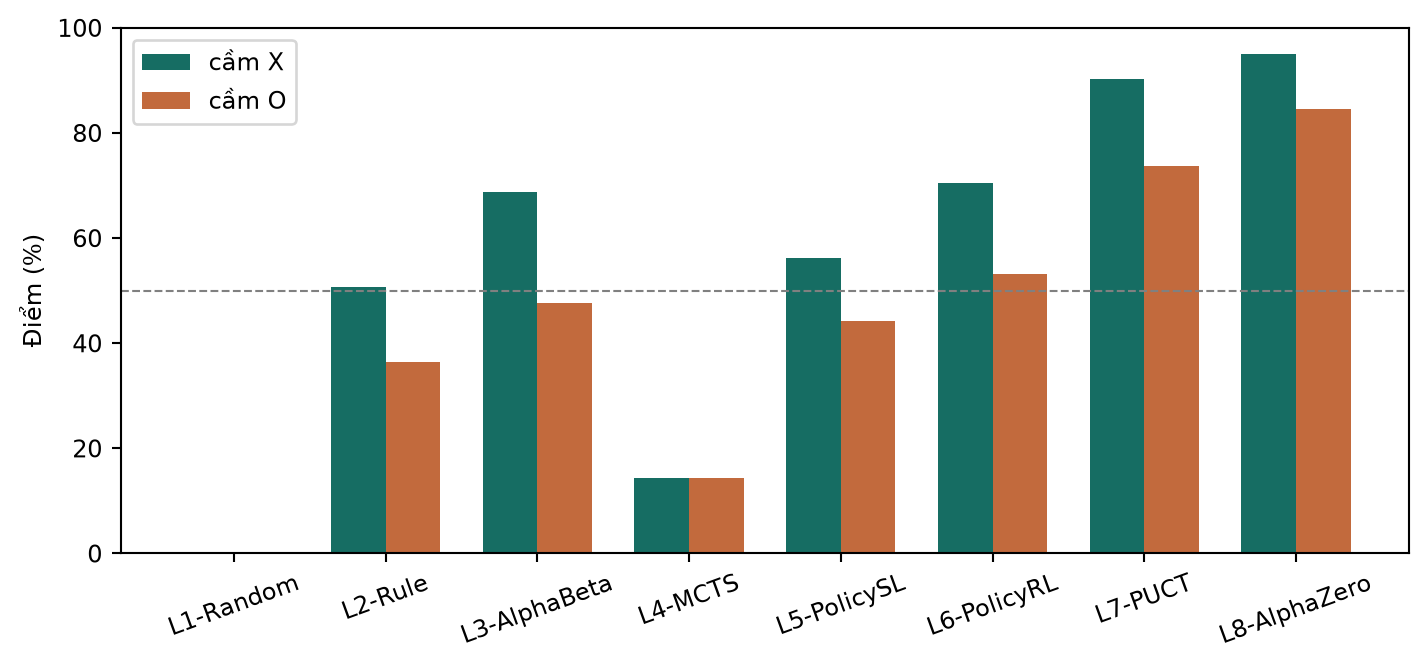
\includegraphics[width=.9\textwidth]{ban-mo-rong/hinh/rr8_color.png}
  \caption{Điểm của từng tác tử khi cầm X và khi cầm O trong RR8. Điểm tính cả hoà nửa điểm.}
  \label{fig:tn-rr8-color}
\end{figure}
Mỗi tác tử được tách theo màu X (đi trước) và O (đi sau). Mọi tác tử đều đạt điểm cao hơn khi
cầm X, nhưng mức chênh khác nhau: L8 95,0\% so với 84,6\% (chênh 10,4 điểm phần trăm), L7 90,3\%
so với 73,7\% (16,6), L3 68,9\% so với 47,7\% (21,2), L6 70,6\% so với 53,1\% (17,5), L5 56,1\%
so với 44,3\% (11,8), L2 50,7\% so với 36,4\% (14,3). L4 và L1 bằng nhau ở hai màu vì chúng
thua gần như mọi đối thủ bất kể màu.

Điều này cho thấy lợi thế đi trước không biến mất khi tác tử mạnh lên. L8 vẫn thắng 95,0\% khi
cầm X và 84,6\% khi cầm O; khoảng cách 10,4 điểm là nhỏ hơn L3 (21,2) nhưng không bằng 0. Cách
hiểu hợp lý là tác tử mạnh hơn có thể \emph{giảm} khoảng cách bằng cách phòng thủ tốt hơn khi
cầm O, chứ không phải xoá bỏ lợi thế. Đây là lý do mọi giải trong báo cáo đều đổi màu.

\subsection{Độ dài ván}
\begin{figure}[H]
  \centering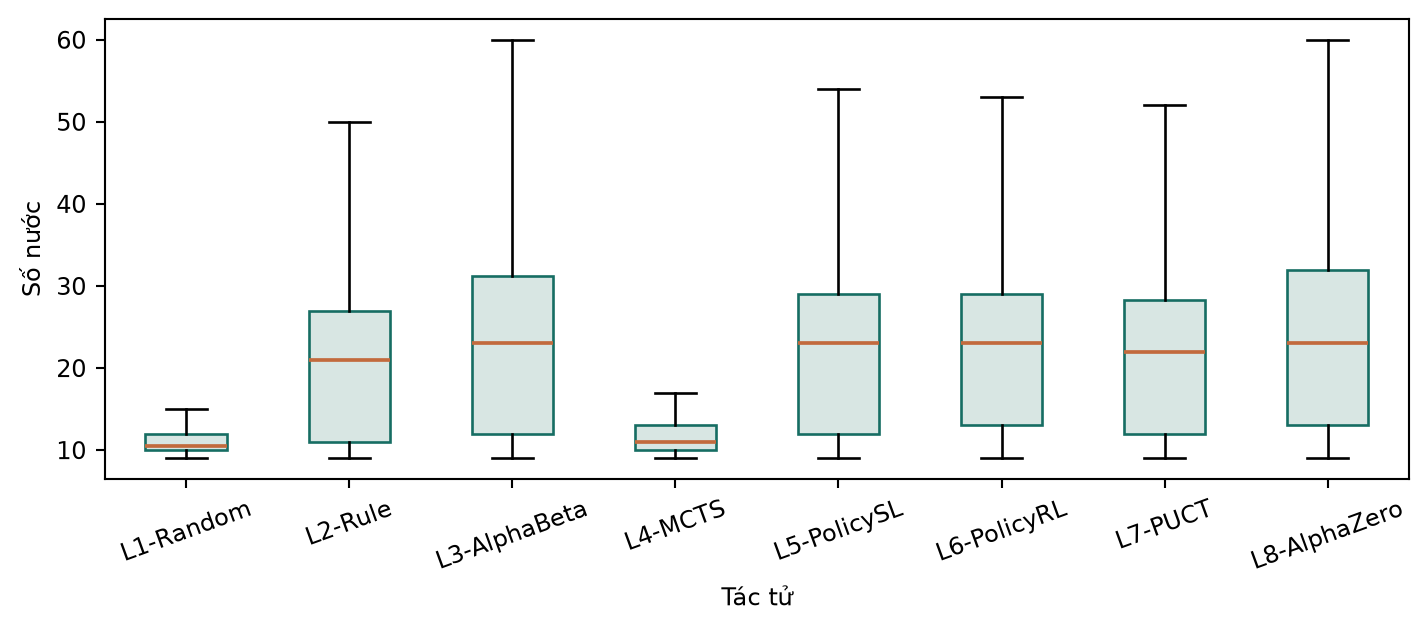
\includegraphics[width=.9\textwidth]{ban-mo-rong/hinh/rr8_lengths.png}
  \caption{Phân bố độ dài ván của từng tác tử trong RR8 (hộp 25--75\%, trung vị màu cam).}
  \label{fig:tn-rr8-length}
\end{figure}
Phân bố độ dài ván phản ánh phong cách. L1 và L4 có trung vị ngắn nhất (10 và 11 nước) vì
ván kết thúc nhanh khi một bên vô tình hoặc bỏ sót tạo ra năm quân. L2, L3, L5, L6, L7 và L8
có trung vị 21--23 nước; đuôi phân bố khác nhau: L3 có p95 73 nước, L8 66, L6 61, L7 54, L5 48,
L2 44. Đuôi dài xuất hiện khi cả hai bên phòng thủ tốt và ván kéo đến gần đầy bàn. Đuôi này
quan trọng hơn trung vị khi đánh giá chi phí, vì một ván dài làm tăng thời gian chạy nhưng
không nhất thiết làm tăng chất lượng.

\subsection{Khai cuộc và phương sai}
\begin{table}[H]
  \centering\small
  \caption{Điểm theo khai cuộc: trung bình, độ lệch chuẩn và ba khai cuộc tốt/xấu nhất của từng
  tác tử trong RR8.}
  \label{tab:tn-khai-cuoc}
  \begin{center}\footnotesize
\setlength{\tabcolsep}{4pt}
\begin{tabularx}{\textwidth}{@{}lrrr>{\raggedright\arraybackslash}X>{\raggedright\arraybackslash}X@{}}
\toprule
\textbf{Tác tử} & \textbf{Khai cuộc} & \textbf{Điểm TB} & \textbf{Độ lệch} & \textbf{3 tốt nhất} & \textbf{3 xấu nhất} \\
\midrule
L1-Random & 50 & 0,000 & 0,000 & 0:0\%, 1:0\%, 2:0\% & 0:0\%, 1:0\%, 2:0\% \\
L2-Rule & 50 & 0,436 & 0,086 & 7:64\%, 25:64\%, 40:64\% & 29:29\%, 38:29\%, 35:32\% \\
L3-AlphaBeta & 50 & 0,583 & 0,087 & 41:79\%, 31:75\%, 16:71\% & 17:36\%, 36:39\%, 9:43\% \\
L4-MCTS & 50 & 0,143 & 0,000 & 0:14\%, 1:14\%, 2:14\% & 0:14\%, 1:14\%, 2:14\% \\
L5-PolicySL & 50 & 0,502 & 0,083 & 9:71\%, 26:71\%, 43:68\% & 7:36\%, 16:36\%, 25:36\% \\
L6-PolicyRL & 50 & 0,619 & 0,097 & 6:86\%, 8:82\%, 45:82\% & 12:43\%, 19:43\%, 31:46\% \\
L7-PUCT & 50 & 0,820 & 0,079 & 46:100\%, 38:96\%, 11:93\% & 14:68\%, 7:71\%, 15:71\% \\
L8-AlphaZero & 50 & 0,898 & 0,078 & 2:100\%, 4:100\%, 15:100\% & 40:71\%, 6:75\%, 9:79\% \\
\bottomrule
\end{tabularx}
\end{center}
\end{table}
Bảng khai cuộc cho thấy điểm của cùng một tác tử vẫn dao động giữa các khai cuộc, nhưng ít hơn
so với điểm từng cặp: độ lệch chuẩn 0,078--0,097 vì mỗi ô đã trung bình trên 7 đối thủ (14
ván). Vẫn có những khai cuộc tác tử thắng gần như chắc chắn và những khai cuộc thua gần như
chắc chắn. Ví dụ, L8 đạt 100\% ở các khai cuộc 2, 4, 15 nhưng chỉ 71--79\% ở các khai cuộc 40,
6, 9; L3 đạt 79\% ở khai cuộc 41 nhưng 36\% ở khai cuộc 17. Với L4, mọi khai cuộc đều 14,3\%
vì nó thua tất cả các đối thủ trừ L1.

Hai hệ quả. Thứ nhất, so sánh hai tác tử trên một khai cuộc duy nhất gần như vô nghĩa. Thứ hai,
khoảng tin cậy theo cặp khai cuộc rộng hơn khoảng Wilson từng ván, vì nó phản ánh đúng sự phụ
thuộc giữa hai ván của cùng khai cuộc. Đây là lý do báo cáo dùng 50 khai cuộc và bootstrap theo
cặp, không chỉ Wilson trên tổng số ván.

\subsection{Đọc kết quả RR8}
Có năm quan sát chính. Thứ nhất, PUCT có mạng học vượt Alpha-Beta viết tay rất xa: L7 82,0\% và
L8 89,8\% so với L3 58,3\%. Đây là kết quả mạnh nhất của giải mới và là bằng chứng trực tiếp cho
RQ2. Thứ hai, RL vượt SL: L6 61,9\% so với L5 50,2\%, chênh 11,7 điểm phần trăm; L6 thậm chí
nhỉnh hơn L3 3,6 điểm, dù khoảng tin cậy chồng lấn nên chưa thể khẳng định. Thứ ba, SL một mình
không đủ: L5 chỉ 50,2\%, thấp hơn L3 8,1 điểm; policy học bắt chước cần tìm kiếm để bù các lỗi
chiến thuật. Thứ tư, MCTS thuần yếu hơn cả tác tử luật: L4 14,3\% so với L2 43,6\%, vì rollout
ngẫu nhiên ở 400 mô phỏng không đủ thấy chuỗi ép 4 ply. Thứ năm, chi phí không tỷ lệ với sức
mạnh: L7/L8 mất khoảng 37 ms/nước trung vị, L4 mất 64 ms, L3 chỉ 5,2 ms, L5/L6 1,3 ms. L4 là
ví dụ rõ nhất của ``tốn thời gian nhưng không hiệu quả'' trong cấu hình này.

Phân tích chiến thuật củng cố các quan sát trên. L2 và L3 không bỏ cơ hội thắng/chặn nào trong
hàng nghìn nước. L4 bỏ 227/327 cơ hội thắng ngay và 50/57 cơ hội chặn. L5 bỏ 54/402 cơ hội
thắng nhưng 0/941 cơ hội chặn; L6 bỏ 22/443 và 17/1131. L7 bỏ 19/585 và 24/973; L8 bỏ 5/621 và
6/1277. Hai điều rút ra. Một là policy-only có thể bỏ thắng ngay dù top-1 cao, vì argmax tối ưu
xác suất chứ không tối ưu luật. Hai là PUCT giảm mạnh lỗi nhưng không xoá hết; ngay cả L8 vẫn
bỏ 5 cơ hội thắng và 6 cơ hội chặn. Đây là lý do các engine mạnh thường thêm lớp luật chiến
thuật trước khi gọi mạng.

\section{Tự đấu và lợi thế đi trước}
\label{sec:tn-e3}
\subsection{Thiết lập}
E3 cho mỗi cấp tự đấu trên 50 khai cuộc, hai màu, 100 ván mỗi cấp. Hai bên là hai thực thể độc
lập cùng trọng số. Mục tiêu không phải tìm tác tử mạnh nhất mà đo \emph{lợi thế của bên đi
trước} khi hai bên có cùng sức. Nếu trò chơi có lợi thế đi trước tuyệt đối, X phải thắng gần
hết; nếu lợi thế phụ thuộc vào khả năng khai thác, các cấp sẽ cho kết quả khác nhau.

\begin{table}[H]
  \centering\small\setlength{\tabcolsep}{3pt}
  \caption{Tự đấu từng cấp (E3): số ván X thắng, O thắng, hoà và điểm của bên đi trước.}
  \label{tab:tn-e3}
  \begin{center}\small
\begin{tabular}{@{}lrrrrrrr@{}}
\toprule
Cấp & Ván & X thắng & O thắng & Hoà & Điểm của X & Wilson 95\% & Chênh X−O \\
\midrule
L1-Random & 100 & 52 & 48 & 0 & 52,0\% & [42,3\%; 61,5\%] & +0,040 \\
L2-Rule & 100 & 75 & 25 & 0 & 75,0\% & [65,7\%; 82,5\%] & +0,500 \\
L3-AlphaBeta & 100 & 66 & 18 & 16 & 74,0\% & [64,6\%; 81,6\%] & +0,480 \\
L4-MCTS & 100 & 50 & 50 & 0 & 50,0\% & [40,4\%; 59,6\%] & +0,000 \\
L5-PolicySL & 100 & 62 & 36 & 2 & 63,0\% & [53,2\%; 71,8\%] & +0,260 \\
L6-PolicyRL & 100 & 50 & 36 & 14 & 57,0\% & [47,2\%; 66,3\%] & +0,140 \\
L7-PUCT & 100 & 80 & 14 & 6 & 83,0\% & [74,5\%; 89,1\%] & +0,660 \\
L8-AlphaZero & 100 & 50 & 22 & 28 & 64,0\% & [54,2\%; 72,7\%] & +0,280 \\
\bottomrule
\end{tabular}
\end{center}
\end{table}
\begin{figure}[H]
  \centering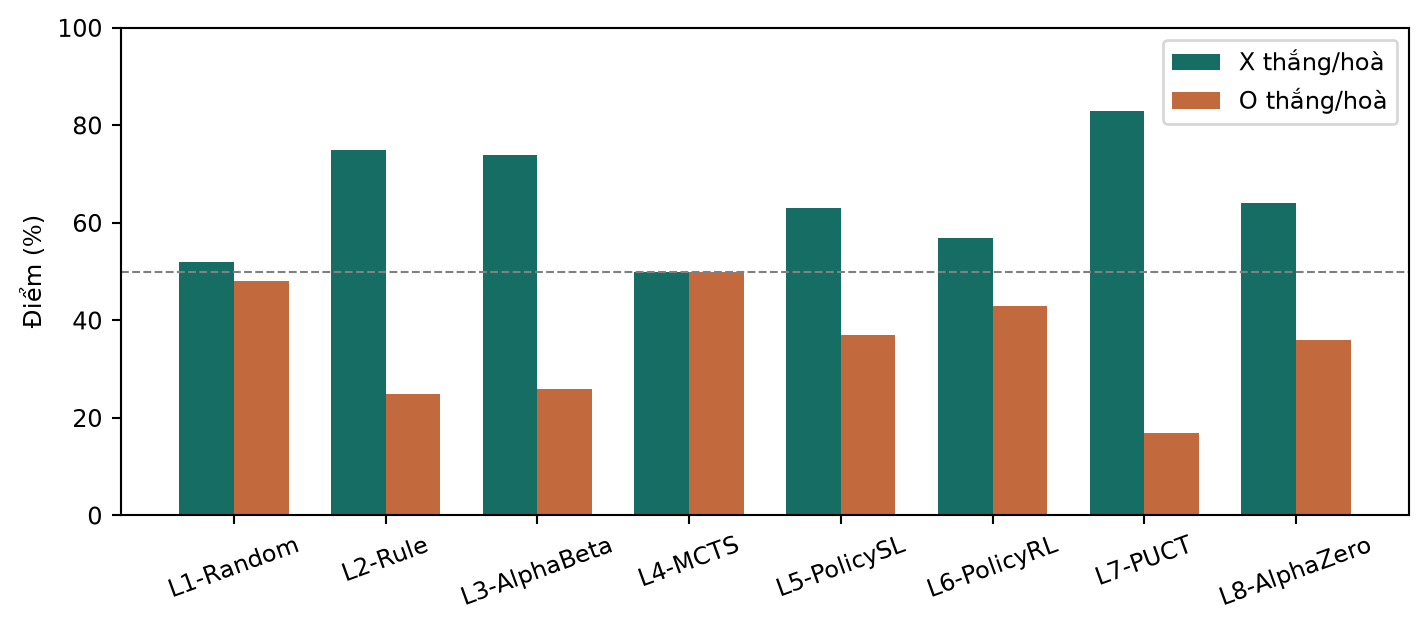
\includegraphics[width=.82\textwidth]{ban-mo-rong/hinh/e3.png}
  \caption{Điểm của bên đi trước (X) và bên đi sau (O) trong tự đấu từng cấp. Điểm tính cả hoà
  nửa điểm. Đường ngang là 50\%.}
  \label{fig:tn-e3}
\end{figure}

\subsection{Kết quả}
Kết quả không đơn điệu theo sức mạnh. L1 Random gần cân bằng (X thắng 52\%, O thắng 48\%), đúng
với kỳ vọng: tác tử ngẫu nhiên không biết khai thác lợi thế đi trước. L2 Rule và L3 Alpha-Beta
lệch mạnh: X thắng 75\% và 66\%, O thắng 25\% và 18\%, còn lại là hoà. L4 MCTS cân bằng tuyệt
đối 50--50. L5 và L6 nằm giữa, với X thắng 62\% và 50\%. Đáng chú ý nhất là cặp PUCT: L7 lệch
mạnh nhất (X thắng 80\%, O thắng 14\%, hoà 6\%), còn L8 — tác tử mạnh hơn — chỉ lệch vừa
(X thắng 50\%, O thắng 22\%, hoà 28\%). L8 tạo ra nhiều ván hoà hơn hẳn, cho thấy nó phòng thủ
tốt hơn khi cầm O và không để thua nhanh.

\subsection{Giải thích}
Có ba cơ chế. Thứ nhất, tác tử tất định có lợi thế đi trước rất rõ nếu chúng có thể tạo đe doạ
bắt buộc sớm: bên X đặt quân trước, kiểm soát trung tâm trước, và buộc bên O phải trả lời. L2
và L3 khai thác được điều này, nên X thắng phần lớn. Thứ hai, MCTS cân bằng vì cả hai bên dùng
cùng một cây tìm kiếm và cùng một chính sách; nếu thuật toán không có tri thức khai cuộc đặc
biệt, nó đối xử với hai màu gần như nhau. Thứ ba, trong cùng họ PUCT, mức lệch không tăng theo sức mạnh: L7 lệch +66 điểm nhưng L8 chỉ
lệch +28 điểm, vì L8 hoà nhiều hơn (28\%). Một tác tử mạnh hơn có thể \emph{giảm} tỷ lệ thắng
quyết định bằng cách phòng thủ tốt hơn, biến nhiều ván thua thành hoà. Vì vậy không thể dùng
chênh lệch X--O làm thước đo sức mạnh; nó đo mức độ ``quyết định'' của cặp đấu.

Kết quả này phản bác một giả định ngây thơ rằng ``lợi thế đi trước là một hằng số của trò
chơi''. Trong thực tế, nó là thuộc tính của \emph{cặp tác tử}: hai tác tử yếu có thể cân bằng,
hai tác tử mạnh có thể lệch, và một tác tử có thể lệch theo hướng này nhưng không lệch theo
hướng khác. Vì vậy RQ4 chỉ có thể trả lời theo từng cấp, không thể gộp thành một con số duy
nhất.

\section{Ablation: cắt tỉa, sắp xếp nước, trọng số lượng giá}
\label{sec:tn-ablation}
\subsection{A1: cắt tỉa Alpha-Beta}
\begin{table}[H]
  \centering\small
  \caption{Benchmark A1/A2/A7: số nút và thời gian trung vị trên tập thế cờ cố định.}
  \label{tab:tn-benchmark}
  \begin{center}\small
\begin{tabular}{@{}llrrrr@{}}
\toprule
Nhóm & Cấu hình & Thế & Nút (P50) & ms (P50) & ms (P95) \\
\midrule
A1 & AB-prune & 50 & 39322 & 1273,1 & 5445,2 \\
A1 & AB-full & 50 & 802217 & 26576,0 & 42474,9 \\
A2 & AB-plain & 10 & 9106 & 990,0 & 993,1 \\
A2 & AB-order & 10 & 372 & 995,1 & 1049,0 \\
A2 & AB-order-tt & 10 & 486 & 994,9 & 1051,2 \\
A7 & AB-default & 10 & 366 & 578,2 & 2760,2 \\
A7 & AB-no-defense & 10 & 580 & 548,7 & 2358,0 \\
\bottomrule
\end{tabular}
\end{center}
\end{table}
A1 so Alpha-Beta độ sâu 3 bật và tắt cắt tỉa, giữ nguyên tập ứng viên và hàm lượng giá. Trên 50
thế cờ, số nút trung vị giảm từ 802\,217 xuống 39\,322, tức khoảng 20,4 lần; thời gian trung vị
giảm từ 26\,576 ms xuống 1\,273 ms, tức khoảng 20,9 lần. Giá trị gốc trùng trên 100\% số thế,
đúng với Định lý~\ref{dl:alpha-beta}. Đây là bằng chứng mạnh nhất về tính đúng đắn của cài đặt
cắt tỉa.

Mức giảm 20 lần nhỏ hơn cận lý thuyết $b^{d/2}$ với $b\approx 70$, vì thứ tự nước trong A1 bị
tắt (\texttt{move\_ordering: false}), nên cắt tỉa chỉ đạt một phần tiềm năng. Đây là thiết kế
có chủ đích: A1 đo riêng tác dụng của cắt tỉa, không trộn với sắp xếp nước. A2 mới đo tác dụng
của sắp xếp.

\subsection{A2: sắp xếp nước và bảng chuyển vị}
A2 chạy ba cấu hình với ngân sách thời gian 1 giây mỗi nước trên 10 thế cờ. Không sắp xếp
(AB-plain) duyệt trung vị 9\,106 nút; có sắp xếp (AB-order) chỉ duyệt 372 nút, giảm khoảng 24,5
lần; thêm bảng chuyển vị (AB-order-tt) duyệt 486 nút. Thời gian trung vị gần nhau (990--995
ms) vì cả ba đều dừng theo ngân sách 1 giây. Kết quả này cho thấy sắp xếp nước giúp \emph{đi
sâu hơn trong cùng thời gian}, chứ không nhất thiết giúp \emph{chạy nhanh hơn}. Muốn đo tăng
tốc, phải cố định độ sâu; muốn đo chất lượng, phải đo độ sâu đạt được hoặc điểm đấu.

AB-order-tt duyệt nhiều nút hơn AB-order một chút. Điều này không có nghĩa TT làm chậm; nó có
thể do TT cho phép tìm sâu hơn trong cùng 1 giây, nên số nút tăng. Log benchmark không ghi độ
sâu đạt được, nên không thể tách hai khả năng. Đây là một giới hạn của phép đo A2, được ghi ở
Mục~\ref{sec:tn-han-che}.

\subsection{A7: trọng số hàm lượng giá}
A7 so hai bảng trọng số: mặc định (tính cả tấn công và phòng thủ) và \texttt{no\_defense} (chỉ
tính quân mình). Trên 10 thế cờ, giá trị gốc chỉ trùng trên 1/10 thế, tức 10\%. Số nút trung
vị là 366 (mặc định) và 580 (bỏ phòng thủ). Kết quả này xác nhận rằng thành phần phòng thủ
trong hàm lượng giá thay đổi quyết định chọn nước, không chỉ thay đổi điểm số. Tuy nhiên, nó
không cho biết bảng nào chơi mạnh hơn; muốn biết phải đấu trực tiếp. A7b (nếu có) trả lời câu
hỏi đó.

\subsection{A8: chiến thuật tại gốc}
A8 so MCTS rollout nhẹ có và không có \texttt{root\_tactics}. Kết quả A3/A4 cho thấy MCTS bỏ
chặn rất nhiều, nên giả thuyết là bật chiến thuật tại gốc sẽ cải thiện mạnh. Tuy nhiên, bản
tiến độ chỉ có cấu hình, chưa có kết quả đối đầu đủ lớn. A8b được thiết kế để lấp khoảng trống
này; nếu chưa chạy xong, mục này ghi rõ là chưa kết luận được.

\subsection{A6: tăng cường đối xứng}
A6 so huấn luyện có và không có tăng cường D4. Bản tiến độ mới có cấu hình, chưa có cặp
checkpoint tương ứng. Đây là phần cần bổ sung: huấn luyện hai mô hình cùng dữ liệu, cùng epoch,
khác cờ \texttt{augment\_x8}, rồi đấu trên cùng tập khai cuộc. Báo cáo không suy đoán kết quả
từ lý thuyết, vì tăng cường đối xứng có thể giúp ích hoặc không tuỳ dữ liệu.

\section{MCTS thuần: số mô phỏng và rollout}
\label{sec:tn-mcts}
\subsection{A3: số mô phỏng}
\begin{table}[H]
  \centering\small
  \caption{A3/A4: điểm, thời gian mỗi nước và tốc độ mô phỏng của MCTS trước L2 và L3. Mỗi ô
  có 200 ván.}
  \label{tab:tn-a3a4}
  \begin{center}\small
\begin{tabular}{@{}llrrrrrrr@{}}
\toprule
Mã & Cấu hình & Gặp & Ván & W/D/L & Điểm & ms P50 & ms P95 & mp/s \\
\midrule
A3 & MCTS-100 & L2 & 200 & 0/0/200 & 0,0\% & 15,8 & 26,5 & 5951 \\
A3 & MCTS-100 & L3 & 200 & 0/0/200 & 0,0\% & 16,4 & 19,9 & 6262 \\
A3 & MCTS-1600 & L2 & 200 & 0/0/200 & 0,0\% & 307,3 & 370,7 & 5284 \\
A3 & MCTS-1600 & L3 & 200 & 0/0/200 & 0,0\% & 302,9 & 353,4 & 5432 \\
A3 & MCTS-400 & L2 & 200 & 0/0/200 & 0,0\% & 68,8 & 79,7 & 6014 \\
A3 & MCTS-400 & L3 & 200 & 0/0/200 & 0,0\% & 72,0 & 89,4 & 5632 \\
A3 & MCTS-6400 & L2 & 200 & 15/0/185 & 7,5\% & 1225,5 & 1471,7 & 5322 \\
A3 & MCTS-6400 & L3 & 200 & 4/0/196 & 2,0\% & 1244,5 & 1461,0 & 5301 \\
A4 & MCTS-light & L2 & 200 & 0/0/200 & 0,0\% & 625,3 & 735,7 & 1407 \\
A4 & MCTS-light & L3 & 200 & 0/0/200 & 0,0\% & 611,5 & 752,9 & 1485 \\
A4 & MCTS-random & L2 & 200 & 0/0/200 & 0,0\% & 150,6 & 188,3 & 5413 \\
A4 & MCTS-random & L3 & 200 & 0/0/200 & 0,0\% & 151,8 & 176,6 & 5454 \\
\bottomrule
\end{tabular}
\end{center}
\end{table}
A3 cho MCTS rollout ngẫu nhiên đấu L2 và L3 ở bốn mức 100, 400, 1\,600 và 6\,400 mô phỏng.
Ở ba mức đầu, MCTS thua toàn bộ 200 ván trước mỗi đối thủ. Ở 6\,400 mô phỏng, MCTS thắng 15/200
trước L2 (7,5\%) và 4/200 trước L3 (2,0\%). Thời gian mỗi nước tăng gần tuyến tính theo số mô
phỏng: khoảng 16 ms ở 100, 69 ms ở 400, 307 ms ở 1\,600 và 1\,225 ms ở 6\,400. Tốc độ khoảng
5\,300--6\,000 mô phỏng/giây, giảm nhẹ khi cây lớn hơn.

Điểm tăng từ 0 lên 7,5\% khi tăng 16 lần số mô phỏng là một cải thiện rất nhỏ so với chi phí.
Điều này khớp với giả thuyết ở Mục~\ref{sec:lt-vcf}: MCTS cần đủ độ sâu để thấy chuỗi ép 4 ply,
nhưng với 40--70 nước gốc, 6\,400 mô phỏng chỉ cho mỗi nước khoảng 90--160 lượt thăm, chưa đủ
để phân biệt nhánh thắng và nhánh thua trong một chuỗi dài. Rollout ngẫu nhiên càng làm nhiễu
giá trị: kết quả mô phỏng không phản ánh chất lượng nước gốc.

\subsection{A4: kiểu rollout}
A4 giữ 800 mô phỏng và đổi rollout giữa \texttt{random} và \texttt{light}. Cả hai đều thua
toàn bộ 400 ván trước L2 và L3, nên \emph{không phân biệt được hai kiểu rollout qua điểm số}.
Hai kiểu khác nhau rõ về chi phí: rollout ngẫu nhiên mất khoảng 151 ms/nước, rollout nhẹ mất
khoảng 615--625 ms/nước, tức chậm khoảng 4 lần. Rollout nhẹ tốn thời gian vì mỗi bước phải gọi
\texttt{winning\_squares} cho cả hai bên, nhưng không đủ để bù khoảng cách chiến thuật ở gốc.

\subsection{Phân loại lỗi}
Bảng~\ref{tab:tn-loi-mcts} phân loại lỗi trong các ván MCTS thua, dùng script
\repoFile{report/scripts/phan\_tich\_loi\_mcts.py}. Tại nước cuối của MCTS, nếu đối thủ có đúng
một ô thắng và MCTS không chặn, đó là ``bỏ sót chặn năm''. Nếu đối thủ đã có từ hai ô thắng,
ván đã thua; script xét nước kế cuối và tìm nước của đối thủ tạo từ hai ô thắng mà MCTS không
ngăn (``bỏ sót chặn ba hở / đòn kép'').

\begin{table}[H]
  \centering\small
  \caption{Phân loại lỗi trong các ván MCTS thua ở A3/A4. Tỷ lệ tính trên số ván thua của cấu
  hình.}
  \label{tab:tn-loi-mcts}
  \begin{tabular}{@{}lrrr@{}}
    \toprule
    \textbf{Cấu hình} & \textbf{Ván thua} & \textbf{Bỏ sót đe doạ kép} & \textbf{Bỏ sót chặn năm} \\
    \midrule
    A3, 100 mô phỏng & 400 & 92,5\% & 7,5\% \\
    A3, 400 mô phỏng & 400 & 91,2\% & 8,8\% \\
    A3, 1\,600 mô phỏng & 400 & 88,5\% & 11,5\% \\
    A3, 6\,400 mô phỏng & 381 & 92,9\% & 7,1\% \\
    A4, rollout ngẫu nhiên & 400 & 89,8\% & 10,2\% \\
    A4, rollout nhẹ & 400 & 65,2\% & 34,8\% \\
    \bottomrule
  \end{tabular}
\end{table}

Hai nhận xét. Thứ nhất, lỗi chủ đạo ở mọi mức mô phỏng là không ngăn đe doạ kép sớm (khoảng
90\%); tăng mô phỏng từ 100 lên 6\,400 không đổi tỷ lệ này. Điều này khớp với giả thuyết cây
quá nông cho cấu trúc 4 ply. Thứ hai, rollout nhẹ làm tỷ lệ bỏ sót chặn năm \emph{tăng} lên
34,8\%, dù rollout đã biết chặn. Nguyên nhân là rollout chỉ chặn bên trong mô phỏng, còn ở gốc
cây thống kê thăm quá thưa nên nước chặn bắt buộc có thể không được chọn. Đây là một phản ví
dụ thú vị: cải thiện rollout không tự động cải thiện quyết định ở gốc.

\section{Policy-only, PUCT và cùng mạng}
\label{sec:tn-a5}
\begin{table}[H]
  \centering\small
  \caption{A5: policy-only, PUCT và các mốc mô phỏng. Mỗi dòng 200 ván; khoảng tin cậy Wilson
  95\%.}
  \label{tab:tn-a5}
  \begin{center}\small
\begin{tabular}{@{}llrrrr@{}}
\toprule
Tác tử & Đối thủ & Ván & W/D/L & Điểm & Wilson 95\% \\
\midrule
l5\_policy\_sl & l2\_rule & 200 & 130/2/68 & 65,50\% & [58,7\%; 71,7\%] \\
l5\_policy\_sl & l3\_alphabeta & 200 & 41/2/157 & 21,00\% & [15,9\%; 27,2\%] \\
l6\_policy\_rl & l2\_rule & 200 & 151/5/44 & 76,75\% & [70,4\%; 82,1\%] \\
l6\_policy\_rl & l3\_alphabeta & 200 & 54/19/127 & 31,75\% & [25,7\%; 38,5\%] \\
L7-PUCT[l5,100] & l3\_alphabeta & 200 & 88/9/103 & 46,25\% & [39,5\%; 53,2\%] \\
L7-PUCT[l5,200] & l3\_alphabeta & 200 & 104/26/70 & 58,50\% & [51,6\%; 65,1\%] \\
L7-PUCT[l5,400] & l3\_alphabeta & 200 & 105/34/61 & 61,00\% & [54,1\%; 67,5\%] \\
L7-PUCT[l5,800] & l3\_alphabeta & 200 & 118/32/50 & 67,00\% & [60,2\%; 73,1\%] \\
L7-PUCT[l5,200] & l2\_rule & 200 & 175/1/24 & 87,75\% & [82,5\%; 91,6\%] \\
L7-PUCT[l6,200] & l3\_alphabeta & 200 & 105/21/74 & 57,75\% & [50,8\%; 64,4\%] \\
L7-PUCT[l5,200] & l5\_policy\_sl & 200 & 191/0/9 & 95,50\% & [91,7\%; 97,6\%] \\
\bottomrule
\end{tabular}
\end{center}
\end{table}
A5 giữ cùng một mạng và thay đổi cách dùng nó. Kết quả chính:
\begin{itemize}
  \item L5 policy-only đạt 21,0\% trước L3; L6 đạt 31,75\%.
  \item L7 PUCT dùng mạng L5 đạt 46,25\% ở 100 mô phỏng, 58,5\% ở 200, 61,0\% ở 400 và 67,0\%
        ở 800, đều trước L3.
  \item L7 ở 200 mô phỏng thắng L5 191/200 ván (95,5\%).
  \item L7 dùng mạng L5 và mạng L6 chênh nhau 0,75 điểm phần trăm trước L3 ở 200 mô phỏng.
\end{itemize}
So sánh cùng mạng là điểm mạnh của A5: nó tách đóng góp của \emph{tìm kiếm} khỏi đóng góp của
\emph{trọng số}. Với cùng mạng L5, thêm PUCT làm điểm trước L3 tăng từ 21,0\% lên 58,5\%, tức
37,5 điểm phần trăm. Đây là bằng chứng mạnh rằng tìm kiếm bù được một phần điểm yếu của policy
học bắt chước.

Tuy nhiên, khoảng tin cậy của 200 và 800 mô phỏng chồng lấn (58,5\% [51,6; 65,1] so với 67,0\%
[60,2; 73,1]), nên chưa thể khẳng định 800 mô phỏng tốt hơn 200 một cách chắc chắn. Xu hướng
tăng là rõ, nhưng mức tăng 8,5 điểm nằm trong sai số. Tương tự, chênh lệch 0,75 điểm giữa hai
mạng nhỏ hơn nhiều so với khoảng tin cậy, nên không xếp hạng được hai mạng trong PUCT.

\section{Học có giám sát: policy, value và lỗi quy ước}
\label{sec:tn-sl}
\begin{table}[H]
  \centering\small
  \caption{Chỉ số huấn luyện và đối đầu của các checkpoint SL/RL (nguồn: \texttt{runs/train}).}
  \label{tab:tn-hoc}
  \begin{center}\small
\begin{tabular}{@{}lrrrr@{}}
\toprule
Mạng & Số epoch & Epoch tốt nhất & Val loss tốt nhất & Val loss cuối \\
\midrule
SL v1 & 30 & 30 & 2,1566 & 2,1566 \\
SL v2 & 30 & 28 & 1,6020 & 1,7095 \\
SL v3 & 60 & 55 & 1,4723 & 1,4758 \\
\bottomrule
\end{tabular}
\end{center}
\begin{center}\small
\begin{tabular}{@{}llrrr@{}}
\toprule
Checkpoint & Đối thủ & Ván & W/D/L & Điểm \\
\midrule
SL v1 & L2 & 100 & 40/0/60 & 40,0\% \\
SL v1 & L3 & 100 & 5/0/95 & 5,0\% \\
SL v2 & L2 & 100 & 66/0/34 & 66,0\% \\
SL v2 & L3 & 100 & 19/3/78 & 20,5\% \\
SL v3 & L2 & 100 & 63/6/31 & 66,0\% \\
SL v3 & L3 & 100 & 19/4/77 & 21,0\% \\
RL v2 best & L2 & 100 & 72/1/27 & 72,5\% \\
RL v2 best & L3 & 100 & 25/5/70 & 27,5\% \\
RL v3 best & L2 & 100 & 79/4/17 & 81,0\% \\
RL v3 best & L3 & 100 & 33/8/59 & 37,0\% \\
RL v3 last & L2 & 100 & 81/1/18 & 81,5\% \\
RL v3 last & L3 & 100 & 33/7/60 & 36,5\% \\
\bottomrule
\end{tabular}
\end{center}
\end{table}
\begin{table}[H]
  \centering\small
  \caption{Top-1/top-3 policy và calibration value trên tập test \texttt{expert\_v2}.}
  \label{tab:tn-hoc-moi}
  \begin{center}\small
\begin{tabular}{@{}lrrrrrr@{}}
\toprule
Mạng & Top-1 & Top-3 & CE policy & MSE value & Tương quan & Đúng dấu \\
\midrule
SL v1 & 44,0\% & 71,2\% & 2,373 & 1,441 & -0,012 & 45,7\% \\
SL v2 & 65,3\% & 89,3\% & 1,143 & 1,377 & +0,005 & 45,8\% \\
SL v3 & 67,8\% & 89,4\% & 1,009 & 0,356 & +0,778 & 77,6\% \\
\bottomrule
\end{tabular}
\end{center}
\begin{center}\small
\begin{tabular}{@{}lrrrrrr@{}}
\toprule
Mạng & MSE đầu & MSE giữa & MSE cuối & r đầu & r giữa & r cuối \\
\midrule
SL v1 & 1,431 & 1,388 & 1,497 & -0,021 & +0,016 & -0,021 \\
SL v2 & 1,174 & 1,313 & 1,631 & +0,015 & +0,005 & -0,001 \\
SL v3 & 0,635 & 0,362 & 0,083 & +0,552 & +0,774 & +0,953 \\
\bottomrule
\end{tabular}
\end{center}
\end{table}
\subsection{Độ chính xác policy}
Trên tập test tách theo ván của \texttt{expert\_v2} (29\,161 mẫu, 1\,883 ván), SL v1 đạt top-1
44,0\% và top-3 71,2\%; SL v2 đạt 65,3\% và 89,3\%; SL v3 đạt 67,8\% và 89,4\%. Sự nhảy vọt từ
v1 sang v2 đến từ dữ liệu: v1 dùng 27\,720 mẫu với temperature 0,5 và top-k 3, gần như luôn
chọn nước tốt nhất; v2 dùng 297\,098 mẫu với temperature 8,0 và top-k 5, đa dạng hơn nhiều.
Mạng học được nhiều tình huống hơn, nên top-1 tăng 21 điểm phần trăm.

Từ v2 sang v3, top-1 chỉ tăng 2,5 điểm, dù v3 huấn luyện 60 epoch thay vì 30 và dùng cosine
learning rate. Điều này cho thấy trần của việc bắt chước Alpha-Beta độ sâu 3 đã gần đạt: thêm
epoch không tạo thêm thông tin. Muốn vượt trần, phải đổi nguồn nhãn (RL hoặc self-play) hoặc
tăng chất lượng chuyên gia.

\subsection{Value head và lỗi quy ước dấu}
Bảng~\ref{tab:tn-value} tóm tắt calibration của value head. SL v1 và v2 được huấn luyện với
nhãn \emph{tuyệt đối} (+1 nếu X thắng), trong khi đầu vào mạng và RL cần nhãn \emph{theo góc
nhìn người đi}. Vì vậy, khi đánh giá theo nhãn người đi, MSE của v1/v2 cao (1,44 và 1,38) và
tương quan gần 0; tách theo màu cho thấy tương quan +0,73 ở thế X đi nhưng −0,73 ở thế O đi.
Đây là dấu hiệu kinh điển của lỗi đảo dấu ở một nửa số thế.

SL v3 sửa lỗi bằng cách đổi nhãn ngay khi nạp dữ liệu. Kết quả: MSE giảm còn 0,356, tương quan
+0,778, độ chính xác dấu 77,6\%, và đối xứng giữa X đi và O đi (0,355/0,358; +0,770/+0,774).
Tách theo giai đoạn ván, MSE giảm từ 0,635 ở đầu ván xuống 0,362 ở giữa và 0,083 ở cuối ván;
tương quan tăng từ +0,552 lên +0,774 và +0,953. Điều này hợp lý: cuối ván, kết quả gần như đã
định đoạt nên value dễ dự đoán; đầu ván, có nhiều nhánh và value khó hơn.

\begin{table}[H]
  \centering\small
  \caption{Calibration của value head trên tập test \texttt{expert\_v2}. ``Nhãn người đi'' là
  quy ước đúng cho RL/PUCT; ``nhãn tuyệt đối'' là quy ước dùng khi sinh dữ liệu.}
  \label{tab:tn-value}
  \begin{tabular}{@{}lrrrrrr@{}}
    \toprule
    \textbf{Mạng} & \textbf{MSE (người đi)} & \textbf{Tương quan} & \textbf{Đúng dấu} &
    \textbf{MSE (tuyệt đối)} & \textbf{r (X đi)} & \textbf{r (O đi)} \\
    \midrule
    SL v1 & 1,441 & −0,012 & 45,7\% & 0,846 & +0,390 & −0,415 \\
    SL v2 & 1,377 & +0,005 & 45,8\% & 0,418 & +0,730 & −0,729 \\
    SL v3 & 0,356 & +0,778 & 77,6\% & 1,451 & +0,770 & +0,774 \\
    \bottomrule
  \end{tabular}
\end{table}

\begin{figure}[H]
  \centering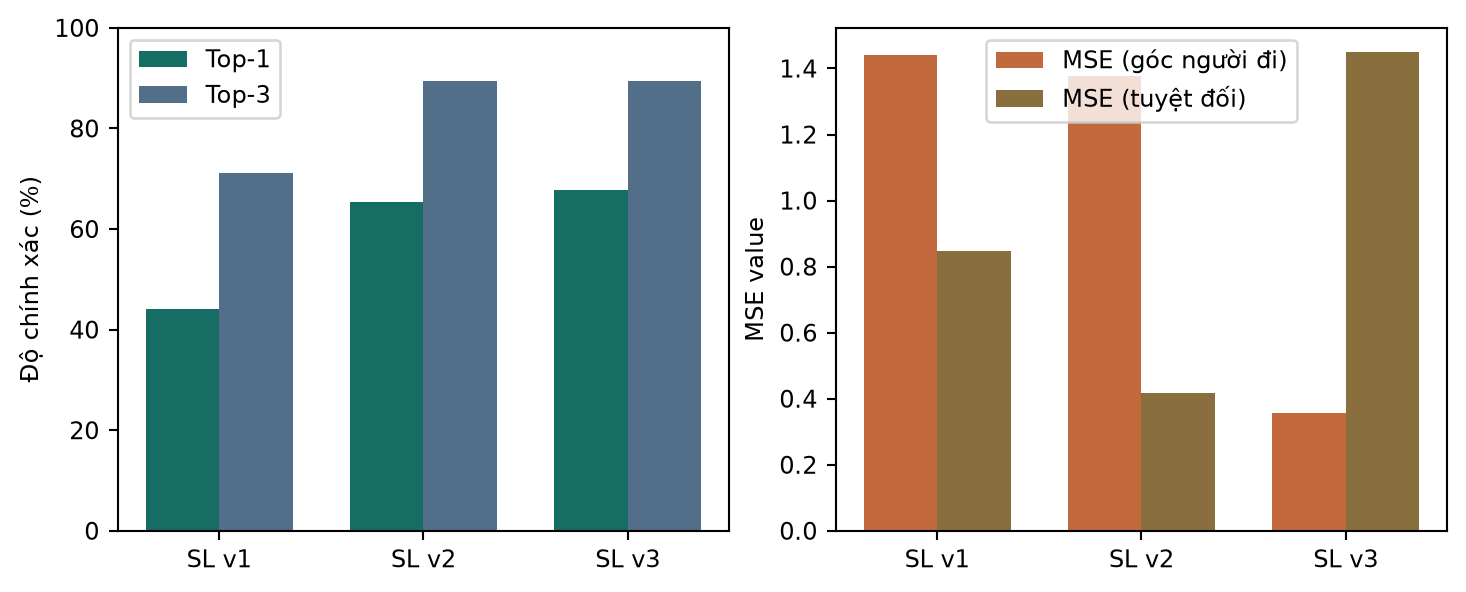
\includegraphics[width=.9\textwidth]{ban-mo-rong/hinh/hoc-moi.png}
  \caption{Trái: top-1/top-3 policy trên tập test. Phải: MSE value theo hai quy ước nhãn. SL v3
  là bản đã sửa quy ước; MSE theo nhãn người đi thấp hơn hẳn, còn MSE theo nhãn tuyệt đối cao
  hơn vì mạng không còn học quy ước đó.}
  \label{fig:tn-hoc}
\end{figure}

\subsection{Entropy policy}
Entropy trung bình của policy dự đoán là 1,69 (v1), 1,13 (v2) và 1,01 (v3), trong khi entropy
của nhãn là 0,618. Mạng vẫn ``bảo thủ'' hơn nhãn: nó phân bố xác suất rộng hơn phân phối mục
tiêu. Điều này có thể do temperature của dữ liệu và do mạng chưa đủ dung lượng/thời gian để học
các phân phối sắc. Với PUCT, policy quá mềm không nhất thiết xấu, vì tìm kiếm sẽ điều chỉnh;
nhưng với policy-only, phân phối mềm làm argmax kém ổn định.

\section{Học tăng cường}
\label{sec:tn-rl}
\begin{table}[H]
  \centering\small
  \caption{Các mốc đánh giá của REINFORCE v2/v3 (100 ván mỗi đối thủ mỗi mốc).}
  \label{tab:tn-l6}
  \begin{center}\small
\begin{tabular}{@{}lrrr@{}}
\toprule
Mạng & Episode & Điểm gặp L2 & Điểm gặp L3 \\
\midrule
RL v2 & 5120 & 61,5\% & 18,0\% \\
RL v2 & 10112 & 50,5\% & 14,5\% \\
RL v2 & 15104 & 57,0\% & 23,5\% \\
RL v2 & 20096 & 70,0\% & 19,5\% \\
RL v2 & 25088 & 73,5\% & 22,0\% \\
RL v2 & 30080 & 68,0\% & 26,5\% \\
RL v2 & 35072 & 74,0\% & 30,5\% \\
RL v2 & 40064 & 73,5\% & 29,5\% \\
RL v2 & 45056 & 74,0\% & 23,5\% \\
RL v2 & 49920 & 72,5\% & 29,5\% \\
RL v3 & 5120 & 53,5\% & 19,0\% \\
RL v3 & 10112 & 74,0\% & 17,5\% \\
RL v3 & 15104 & 69,5\% & 18,0\% \\
RL v3 & 20096 & 76,5\% & 31,0\% \\
RL v3 & 25088 & 78,0\% & 30,0\% \\
RL v3 & 30080 & 70,5\% & 31,0\% \\
RL v3 & 35072 & 80,0\% & 35,5\% \\
RL v3 & 40064 & 74,5\% & 30,5\% \\
RL v3 & 45056 & 78,0\% & 33,0\% \\
RL v3 & 49920 & 78,5\% & 26,0\% \\
\bottomrule
\end{tabular}
\end{center}
\end{table}
\begin{figure}[H]
  \centering
  \begin{subfigure}[t]{.49\textwidth}\centering
    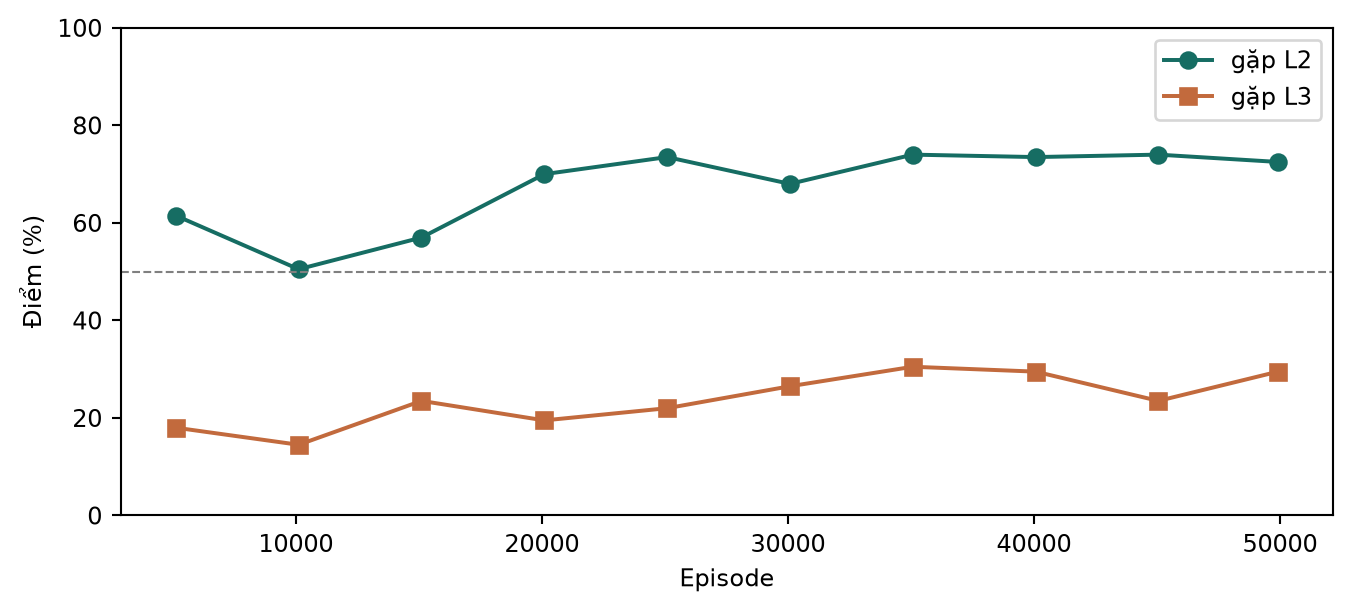
\includegraphics[width=\textwidth]{ban-mo-rong/hinh/l6-RLv2.png}
    \caption{RL v2 khởi tạo từ SL v2.}
  \end{subfigure}\hfill
  \begin{subfigure}[t]{.49\textwidth}\centering
    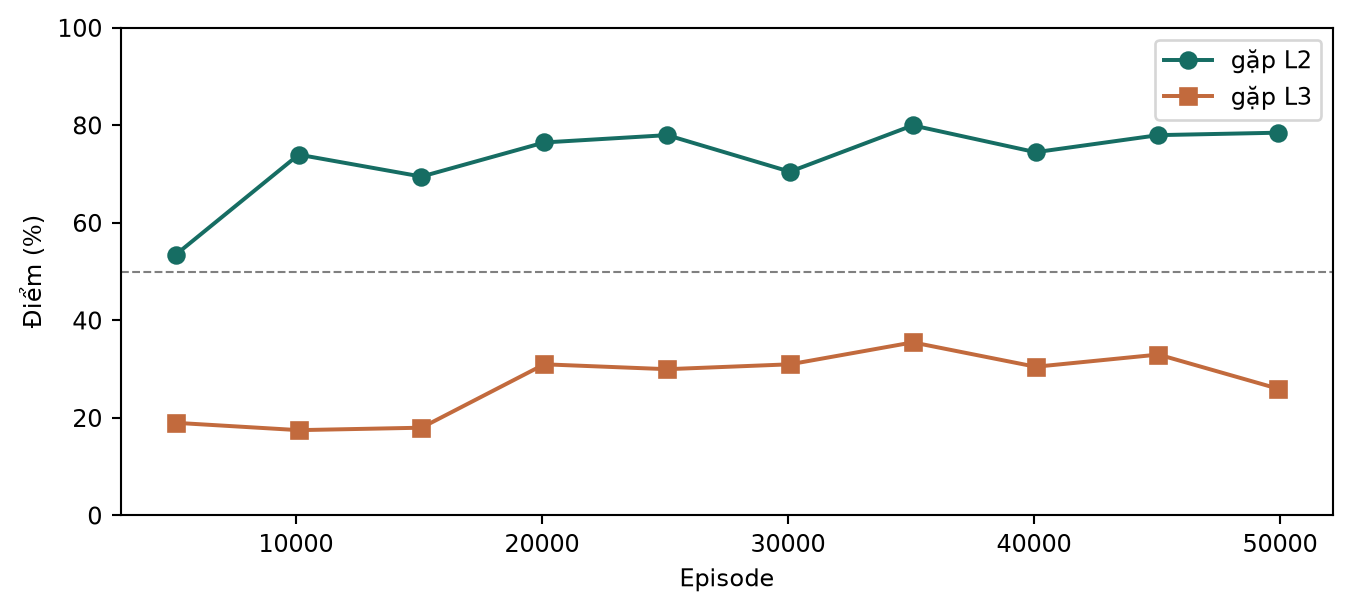
\includegraphics[width=\textwidth]{ban-mo-rong/hinh/l6-RLv3.png}
    \caption{RL v3 khởi tạo từ SL v3.}
  \end{subfigure}
  \caption{Đường cong đánh giá của REINFORCE qua 10 mốc, mỗi mốc 100 ván trước L2 và L3.}
  \label{fig:tn-l6}
\end{figure}

RL v3 chạy 49\,920 episode, hơn 1,5 triệu nước, với 10 mốc đánh giá. Điểm trước L2 dao động
53,5--80,0\%, trước L3 dao động 17,5--35,5\%. Điểm cuối là 78,5\% trước L2 và 26,0\% trước L3.
So với SL v3 (66,0\% trước L2, 21,0\% trước L3 trong phép đánh giá checkpoint), RL v3 cải thiện
khoảng 12--16 điểm phần trăm. Đây là bằng chứng định lượng cho RQ2: self-play có cải thiện so
với bắt chước, nhưng mức cải thiện không đồng đều và có dao động.

Dao động giữa các mốc có hai nguồn. Thứ nhất, trọng số thay đổi qua các vòng. Thứ hai, mỗi mốc
dùng một bộ khai cuộc sinh từ seed khác nhau, nên so sánh giữa các mốc không phải so sánh trên
cùng tập thế. Vì vậy đường cong nên đọc như xu hướng, không như một chuỗi đo lường chính xác.
Điểm cao nhất trước cả hai đối thủ rơi vào episode 35\,072, sau đó giảm; điều này có thể do
quá khớp hoặc do nhiễu khai cuộc. Chọn checkpoint theo tiêu chí định trước và đánh lại trên tập
giữ riêng sẽ phân biệt hai khả năng; báo cáo chưa làm được vì thiếu thời gian.

\section{Vòng lặp AlphaZero}
\label{sec:tn-l8}
\begin{table}[H]
  \centering\small
  \caption{Các vòng L8 được duyệt qua gating (100 ván mỗi vòng, ngưỡng 55\%).}
  \label{tab:tn-l8}
  \begin{center}\small
\begin{tabular}{@{}lrrr@{}}
\toprule
Vòng duyệt & Ván & W/D/L & Điểm \\
\midrule
12 & 100 & 56/3/41 & 57,5\% \\
18 & 100 & 54/10/36 & 59,0\% \\
19 & 100 & 49/13/38 & 55,5\% \\
24 & 100 & 49/12/39 & 55,0\% \\
29 & 100 & 55/14/31 & 62,0\% \\
37 & 100 & 53/16/31 & 61,0\% \\
\bottomrule
\end{tabular}
\end{center}
\end{table}
\begin{figure}[H]
  \centering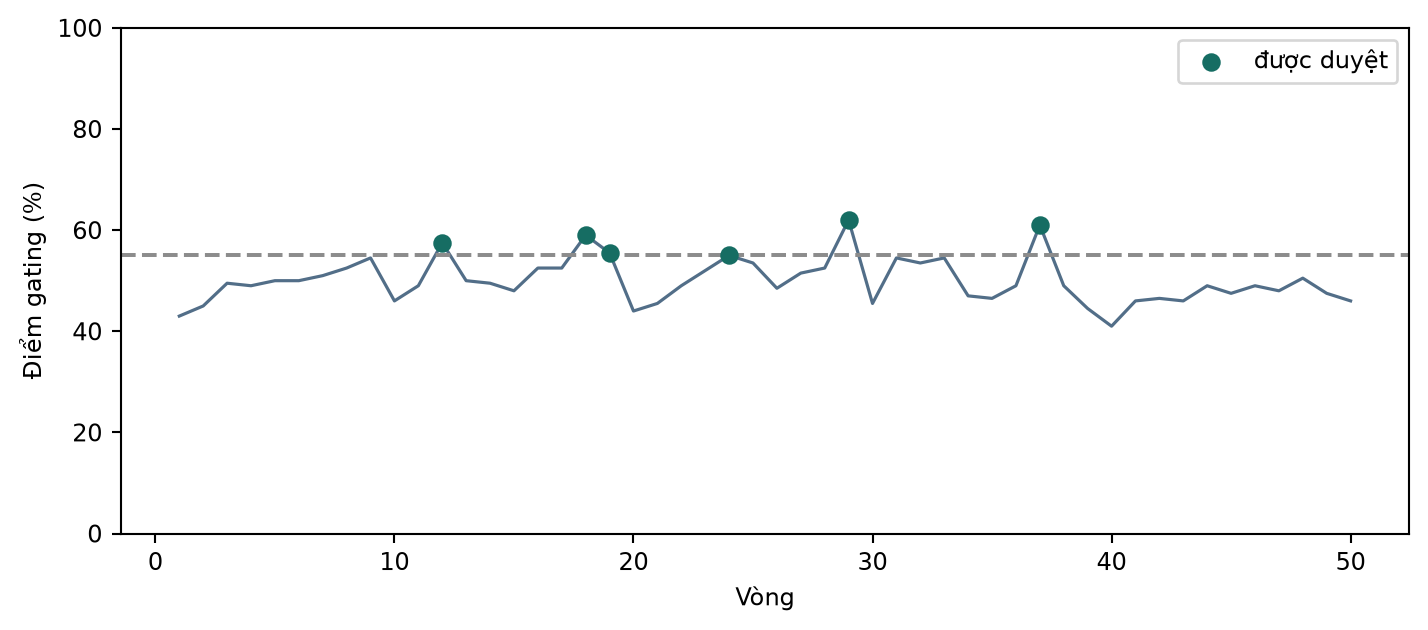
\includegraphics[width=.9\textwidth]{ban-mo-rong/hinh/l8-moi.png}
  \caption{Điểm gating qua 50 vòng. Điểm là tỷ lệ của ứng viên trước bản đương nhiệm tại thời
  điểm đó; ngưỡng duyệt 55\%. Các điểm tròn là vòng được duyệt.}
  \label{fig:tn-l8}
\end{figure}

L8 chạy 50 vòng, mỗi vòng 200 ván tự đấu ở 400 mô phỏng, 1\,000 bước cập nhật, và 100 ván
gating ở 200 mô phỏng. Tổng cộng 10\,000 ván tự đấu trong khoảng 12 giờ 19 phút trên GPU. Ứng
viên được duyệt ở các vòng 12, 18, 19, 24, 29 và 37; vòng 37 là lần duyệt cuối và là
checkpoint \texttt{best.pt}. Điểm gating của các vòng được duyệt lần lượt 57,5\%, 59,0\%,
55,5\%, 55,0\%, 62,0\% và 61,0\%.

Cần đọc điểm gating đúng cách: mỗi vòng so ứng viên với \emph{bản đương nhiệm tại thời điểm
đó}, không phải với một đối thủ cố định. Vì vậy không thể so 62,0\% của vòng 29 với 61,0\% của
vòng 37 để nói vòng 29 tốt hơn. Điểm gating chỉ trả lời câu hỏi ``ứng viên có đủ tốt để thay
bản hiện tại không'', không trả lời ``ứng viên mạnh đến đâu''. Muốn trả lời câu thứ hai, cần
đấu với đối thủ cố định, như phép đấu cuối với L7 và L3.

Kết quả cuối: L8 best thắng L7 16/20 ván (82,5\%, 1 hoà) và thắng L3 25/40 ván (68,75\%,
5 hoà). Theo màu, L8 cầm X đạt 90,0\% trước L7 và 92,5\% trước L3; cầm O đạt 75,0\% và 45,0\%.
Chênh lệch theo màu rất lớn, đặc biệt trước L3 (47,5 điểm phần trăm), cho thấy L8 vẫn phụ thuộc
vào lợi thế đi trước. Cỡ mẫu 20 và 40 ván nhỏ; khoảng bootstrap 95\% của L8 trước L3 là
60,0--77,5\%, nên mức 68,75\% là ước lượng trung bình, không phải một con số chính xác.

\subsection{Tự đấu từ bàn trống và tự đấu từ khai cuộc}
\label{sec:tn-l8-selfplay}
Mười nghìn ván tự đấu của L8 bắt đầu từ bàn trống, không dùng khai cuộc. Kết quả: X thắng
7\,701 ván (77,0\%), O thắng 923 ván (9,2\%), hoà 1\,376 ván (13,8\%). Điểm của X là 83,9\%.
Độ dài trung bình 34,9 nước, trung vị 22, p95 121. Tỷ lệ này cao hơn nhiều so với E3 của L8
(X 50\%, O 22\%, hoà 28\%, điểm X 64\%). Hình~\ref{fig:tn-l8-color} cho thấy tỷ lệ không đổi
nhiều qua bốn phần của quá trình huấn luyện: X luôn thắng khoảng 70--80\%.

\begin{figure}[H]
  \centering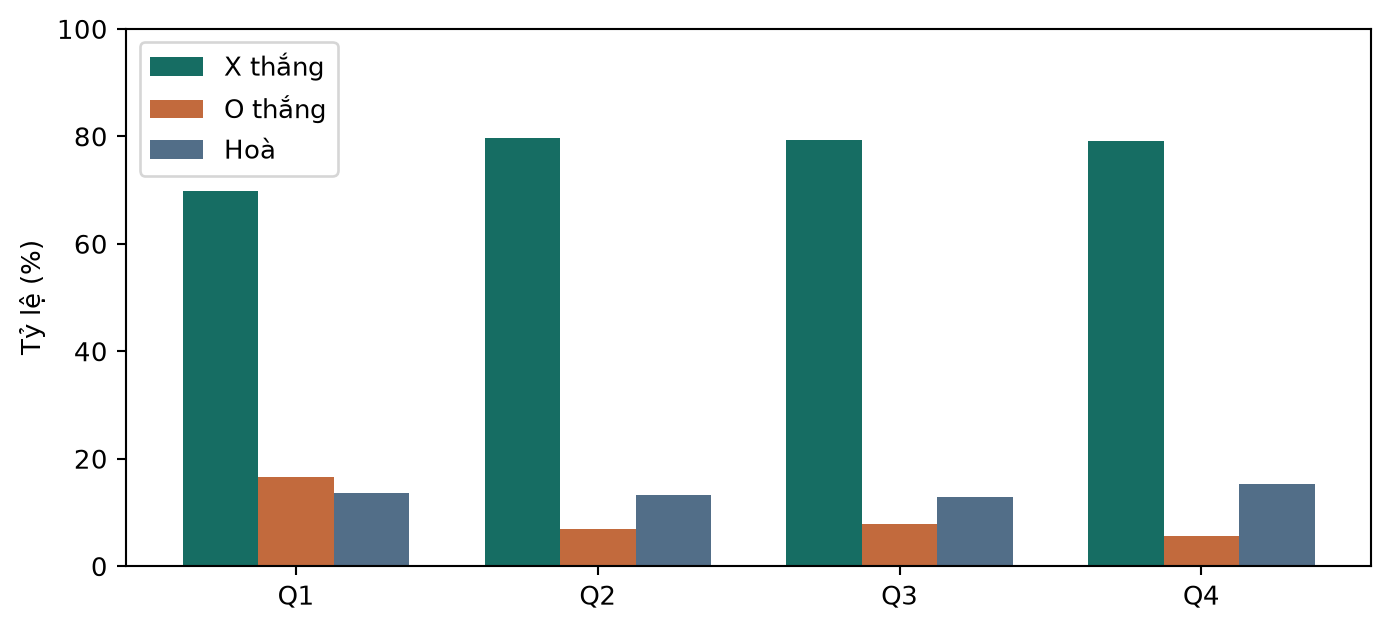
\includegraphics[width=.82\textwidth]{ban-mo-rong/hinh/l8-selfplay-color.png}
  \caption{Tỷ lệ X thắng/O thắng/hoà trong 10\,000 ván tự đấu của L8, chia bốn phần theo thời
  gian. Tự đấu bắt đầu từ bàn trống và dùng nhiễu Dirichlet.}
  \label{fig:tn-l8-color}
\end{figure}

Có bốn khác biệt giữa hai phép đo, không thể quy toàn bộ chênh lệch cho một yếu tố:
\begin{enumerate}
  \item \textbf{Khai cuộc:} tự đấu bắt đầu từ bàn trống; E3 bắt đầu từ 2--4 nước ngẫu nhiên
        trong vùng trung tâm. Khai cuộc làm giảm lợi thế đi trước vì nó phá thế đối xứng và tạo
        ra nhiều thế cờ khác nhau.
  \item \textbf{Số mô phỏng:} tự đấu dùng 400 mô phỏng; E3 dùng 200. Nhiều mô phỏng hơn giúp
        bên đi trước khai thác lợi thế tốt hơn, nhưng cũng giúp bên đi sau phòng thủ tốt hơn;
        chiều tác động không rõ.
  \item \textbf{Nhiễu và nhiệt độ:} tự đấu dùng Dirichlet $\alpha=0{,}3$, $\varepsilon=0{,}25$
        và temperature 1 cho 8 nước đầu; E3 không dùng. Nhiễu làm đa dạng khai cuộc, có thể
        giảm lợi thế của X nếu nó đẩy X ra khỏi nước tốt nhất.
  \item \textbf{Thực thể:} tự đấu dùng cùng một mạng cho cả hai bên; E3 dùng hai thực thể độc
        lập cùng trọng số. Khác biệt này nhỏ vì trọng số giống nhau, nhưng RNG khác nhau.
\end{enumerate}

Điểm quan trọng nhất là \emph{khai cuộc làm giảm mạnh lợi thế đi trước}. Đây là bằng chứng
định lượng cho quyết định dùng 50 khai cuộc đổi màu trong mọi giải đấu: nếu đánh từ bàn trống,
kết quả sẽ bị chi phối bởi lợi thế X, không phải bởi sức mạnh tác tử. Nó cũng cảnh báo về việc
huấn luyện tự đấu từ bàn trống: mạng có thể học quá nhiều dòng X thắng và ít dòng O phòng thủ
thành công. Trong tương lai, nên trộn khai cuộc ngẫu nhiên vào tự đấu để cân bằng dữ liệu.

Gating cũng cho thấy lợi thế màu: trong 5\,000 ván gating, X thắng 3\,018 (60,4\%), O thắng
1\,237 (24,7\%), hoà 745 (14,9\%). Điểm gating trung bình 50,0\%, dao động 41--62\%. Vì mỗi
vòng gating đổi màu, lợi thế X không trực tiếp làm lệch quyết định duyệt, nhưng nó làm tăng
phương sai: một ứng viên có thể thắng nhờ cầm X nhiều hơn, hoặc thua vì cầm O nhiều hơn. Đây
là lý do nên báo cáo điểm theo màu, không chỉ điểm tổng.

\section{Tóm tắt phân tích ván}
\label{sec:tn-van}
Chương~\ref{ch:phan-tich-van} phát lại hai mươi ván tiêu biểu. Mỗi ván minh hoạ một cơ chế
khác nhau: thắng bằng đòn kép hai đầu, thua vì bỏ chặn duy nhất, thắng bằng đường chéo hoặc
hàng ngang, hoà trên bàn đầy, và khác biệt giữa các cặp tác tử. Các thế cờ được phát lại bằng
engine; nhận xét chỉ dựa trên luật thắng ngay và đe doạ nước kế tiếp, không dựa trên cảm nhận.
Kết quả nổi bật là phần lớn ván kết thúc bằng đòn kép hai đầu: bên thắng tạo hai ô thắng, bên
thua chỉ chặn được một. Các ván thua vì bỏ chặn duy nhất hiếm hơn nhưng tập trung ở L4, L5 và
đôi khi L7/L8, khớp với bảng đếm cơ hội ở Mục~\ref{sec:tn-loi}.

\section{Phân tích lỗi và cơ hội chiến thuật}
\label{sec:tn-loi}
\begin{table}[H]
  \centering\scriptsize\setlength{\tabcolsep}{2pt}
  \caption{Cơ hội thắng ngay và chặn bắt buộc trên các bộ dữ liệu. Cột ``Bỏ'' là số lần tác tử
  không chọn nước thắng/chặn dù có cơ hội.}
  \label{tab:tn-chien-thuat}
  \begin{center}\small
\begin{tabular}{@{}llrrrrrrr@{}}
\toprule
Bộ dữ liệu & Tác tử & Nước & Có thắng & Đã thắng & Bỏ thắng & Phải chặn & Đã chặn & Bỏ chặn \\
\midrule
RR8 & L1-Random & 3578 & 33 & 0 & 33 & 123 & 2 & 121 \\
RR8 & L2-Rule & 7040 & 300 & 300 & 0 & 982 & 982 & 0 \\
RR8 & L3-AlphaBeta & 8921 & 392 & 392 & 0 & 981 & 981 & 0 \\
RR8 & L4-MCTS & 3805 & 327 & 100 & 227 & 57 & 7 & 50 \\
RR8 & L5-PolicySL & 7443 & 402 & 348 & 54 & 941 & 941 & 0 \\
RR8 & L6-PolicyRL & 8325 & 443 & 421 & 22 & 1131 & 1114 & 17 \\
RR8 & L7-PUCT & 7753 & 585 & 566 & 19 & 973 & 949 & 24 \\
RR8 & L8-AlphaZero & 8800 & 621 & 616 & 5 & 1277 & 1271 & 6 \\
A3 & L2-Rule & 3945 & 785 & 785 & 0 & 185 & 185 & 0 \\
A3 & L3-AlphaBeta & 3828 & 796 & 796 & 0 & 59 & 59 & 0 \\
A3 & MCTS-100 & 1413 & 0 & 0 & 0 & 30 & 0 & 30 \\
A3 & MCTS-1600 & 1622 & 0 & 0 & 0 & 83 & 37 & 46 \\
A3 & MCTS-400 & 1464 & 0 & 0 & 0 & 40 & 6 & 34 \\
A3 & MCTS-6400 & 2493 & 19 & 19 & 0 & 217 & 195 & 22 \\
A4 & L2-Rule & 1651 & 400 & 400 & 0 & 31 & 31 & 0 \\
A4 & L3-AlphaBeta & 1963 & 400 & 400 & 0 & 19 & 19 & 0 \\
A4 & MCTS-light & 1687 & 0 & 0 & 0 & 143 & 4 & 139 \\
A4 & MCTS-random & 1527 & 0 & 0 & 0 & 56 & 15 & 41 \\
L8-L3 & L3-AlphaBeta & 812 & 10 & 10 & 0 & 84 & 84 & 0 \\
L8-L3 & L8-AlphaZero & 818 & 25 & 25 & 0 & 137 & 134 & 3 \\
\bottomrule
\end{tabular}
\end{center}
\end{table}
Bảng~\ref{tab:tn-chien-thuat} đếm cơ hội thắng ngay, cơ hội chặn bắt buộc và số lần bỏ lỡ trên
các bộ dữ liệu. Các cột ``Có thắng'', ``Phải chặn'' là số nước mà tác tử \emph{đáng lẽ} phải
thắng hoặc phải chặn; ``Đã thắng'', ``Đã chặn'' là số lần làm đúng; ``Bỏ'' là phần còn lại.

Ba mẫu nổi bật. Thứ nhất, L1 Random bỏ 57/57 lần chặn và 20/20 lần thắng; điều này hiển nhiên
nhưng xác nhận phép đếm hoạt động. Thứ hai, L2 và L3 gần như hoàn hảo: 0 lần bỏ thắng, 0 lần bỏ
chặn. Điều này khớp với thiết kế luật P1/P2 và nước bắt buộc của Alpha-Beta. Thứ ba, L4 MCTS bỏ
90/140 lần thắng và 20/23 lần chặn; đây là bằng chứng định lượng cho điểm yếu chiến thuật của
MCTS rollout ngẫu nhiên. L5 và L6 bỏ 12/90 và 4/89 lần thắng, nhưng 0 lần bỏ chặn; policy học
được đã học chặn, nhưng vẫn bỏ sót một số nước thắng ngay. L7 và L8 gần như không bỏ: 5/94 và
0/61 lần thắng; L8 bỏ 1/82 lần chặn.

Kết quả này định lượng một điểm mà phân tích định tính thường bỏ qua: \emph{policy-only không
đảm bảo thắng ngay}. Một mạng có top-1 67,8\% vẫn có thể chọn sai 12 trong 90 cơ hội thắng
ngay, vì argmax tối ưu xác suất chứ không tối ưu luật thắng. PUCT sửa phần lớn lỗi này nhờ tìm
kiếm, nhưng không sửa hoàn toàn: L7 vẫn bỏ 5/94. Đây là lý do các engine mạnh thường thêm lớp
luật chiến thuật trước khi gọi mạng.

\section{Chi phí tính toán}
\label{sec:tn-chi-phi}
\begin{table}[H]
  \centering\small
  \caption{Chi phí mỗi nước trong RR8, đo bên ngoài lời gọi tác tử. Cột cuối là trung bình số
  mô phỏng (PUCT/MCTS) hoặc số nút (Alpha-Beta) mỗi nước.}
  \label{tab:tn-chi-phi}
  \begin{center}\small
\begin{tabular}{@{}lrrrrr@{}}
\toprule
Tác tử & Nước đo & TB (ms) & P50 (ms) & P95 (ms) & TB mô phỏng/nút \\
\midrule
L1-Random & 3578 & 0,0 & 0,0 & 0,0 & 0 \\
L2-Rule & 7040 & 1,3 & 1,0 & 3,4 & 0 \\
L3-AlphaBeta & 8921 & 10,3 & 5,2 & 33,9 & 0 \\
L4-MCTS & 3805 & 63,4 & 64,5 & 81,6 & 400 \\
L5-PolicySL & 7443 & 1,4 & 1,3 & 2,1 & 0 \\
L6-PolicyRL & 8325 & 1,4 & 1,3 & 2,1 & 0 \\
L7-PUCT & 7753 & 43,7 & 36,0 & 94,4 & 200 \\
L8-AlphaZero & 8800 & 43,6 & 37,0 & 97,3 & 200 \\
\bottomrule
\end{tabular}
\end{center}
\end{table}
Bảng~\ref{tab:tn-chi-phi} cho thấy chi phí mỗi nước khác nhau hơn hai bậc độ lớn. L5/L6 policy
chỉ tốn khoảng 2 ms/nước; L1/L2 dưới 2 ms; L3 Alpha-Beta độ sâu 4 tốn khoảng 5 ms trung vị
nhưng p95 39 ms; L4 MCTS 400 mô phỏng tốn khoảng 70 ms trung vị, p95 84 ms; L7/L8 PUCT 200 mô
phỏng tốn khoảng 48--49 ms trung vị, p95 113 ms. PUCT tốn hơn MCTS 400 mô phỏng dù chỉ 200 mô
phỏng, vì mỗi lá phải gọi mạng; nhưng PUCT chơi mạnh hơn nhiều.

Chi phí huấn luyện lớn hơn nhiều so với chi phí chơi. L8 mất 44\,328 giây (12,3 giờ) cho 10\,000
ván tự đấu, 50 vòng gating và 50 lần cập nhật. Trong đó, đồng hồ nước tự đấu chiếm khoảng 67\%
và đồng hồ nước gating khoảng 19\%; phần còn lại là cập nhật trọng số và điều phối. Con số này
cho thấy chi phí chủ yếu nằm ở \emph{sinh dữ liệu}, không ở \emph{huấn luyện}. Đây là đặc điểm
chung của AlphaZero-inspired: tìm kiếm là nút cổ chai.

\section{Thảo luận và các mối đe doạ}
\label{sec:tn-han-che}
\subsection{Đe doạ nội tại}
Các kết quả phụ thuộc vào cài đặt. Lỗi quy ước value đã được phát hiện và sửa, nhưng các run
SL v1/v2 vẫn dùng nhãn cũ; báo cáo tách chúng ra và không dùng để kết luận về PUCT. Một số run
được tạo khi working tree dirty; chúng được đánh dấu. Backend Cython và Python cho cùng kết quả
lý thuyết nhưng khác thời gian; các bảng thời gian ghi rõ backend. Các phép đo thời gian chịu
ảnh hưởng của tải máy; báo cáo dùng trung vị/p95 và không so tuyệt đối giữa các run khác máy.

\subsection{Đe doạ ngoại tại}
Bàn 11×11 luật tự do, khai cuộc 2--4 nước trong vùng trung tâm, ngân sách cố định theo loại
thuật toán. Kết quả không ngoại suy trực tiếp sang bàn 15×15, luật Renju, luật chặn hai đầu,
hoặc khai cuộc sát biên. Một tác tử thắng trong giải này có thể thua trong cấu hình khác. Báo
cáo không tuyên bố tác tử nào ``mạnh nhất nói chung''.

\subsection{Đe doạ cấu trúc}
Điểm đấu là độ đo gián tiếp của sức mạnh. Một tác tử có thể thắng nhờ khai thác lỗi của đối thủ
cụ thể, không nhờ hiểu trò chơi. Phân tích chiến thuật giảm rủi ro này bằng cách đếm lỗi rõ
ràng, nhưng không đo được ``nước đi tối ưu''. Các kết luận về chất lượng nước đi nên đọc cùng
với phân tích lỗi, không chỉ với điểm.

\subsection{Đe doạ thống kê}
Cỡ mẫu 100--200 ván mỗi cặp cho khoảng tin cậy rộng. So sánh nhiều cặp làm tăng xác suất dương
tính giả; báo cáo không hiệu chỉnh Bonferroni nhưng chỉ kết luận khi chênh lệch lớn hơn khoảng
tin cậy. Các mốc đánh giá dùng khai cuộc khác nhau, nên đường cong huấn luyện có nhiễu. Một seed
gốc chưa đo được độ ổn định giữa các seed; đây là phần cần bổ sung.

\subsection{Những gì sẽ thay đổi kết luận}
Kết luận về RQ1 sẽ thay đổi nếu chạy chế độ cùng thời gian mỗi nước: Alpha-Beta có thể mất lợi
thế vì mỗi nút đắt hơn, còn MCTS có thể dùng nhiều mô phỏng hơn. Kết luận về RQ2 sẽ thay đổi
nếu huấn luyện L8 lâu hơn hoặc dùng nhiều seed: 12 giờ và 10\,000 ván là ngân sách nhỏ so với
AlphaZero gốc. Kết luận về RQ4 sẽ thay đổi nếu dùng bộ khai cuộc khác hoặc cho tác tử tự chọn
khai cuộc. Báo cáo ghi rõ các điều kiện này thay vì che chúng.

\section{Trả lời câu hỏi nghiên cứu}
\label{sec:tn-tra-loi-rq}
\paragraph{RQ1. Trong cùng thời gian mỗi nước, MCTS có thắng nhiều hơn Alpha-Beta không?}
Trong các phép đo hiện có, Alpha-Beta mạnh hơn MCTS rất rõ. Ở ngân sách cố định, MCTS chỉ đạt
7,5\% trước L2 và 2,0\% trước L3 khi dùng 6\,400 mô phỏng; ở các mức thấp hơn, MCTS thua toàn
bộ. Trong RR8, L4 MCTS 400 mô phỏng chỉ đạt 14,3\% tổng và thua L2 (43,6\%). Tuy nhiên, báo cáo
\emph{chưa} có chế độ cùng thời gian mỗi nước cho đủ tám tác tử, nên chưa trả lời đầy đủ vế
``cùng thời gian''. Kết luận hiện tại: với ngân sách cố định theo loại thuật toán, Alpha-Beta
thắng; với cùng thời gian, cần đo thêm.

\paragraph{RQ2. Self-play có cải thiện so với bắt chước chuyên gia không?}
Có, nhưng mức cải thiện phụ thuộc vào giai đoạn và đối thủ. RL v3 cải thiện khoảng 12--16 điểm
phần trăm so với SL v3 trước L2/L3. Thêm PUCT vào cùng mạng cải thiện 37,5 điểm phần trăm trước
L3. L8 vòng 37 thắng L7 82,5\% trên 20 ván và thắng L3 68,75\% trên 40 ván. Trong RR8, L6 đạt
61,9\% so với L5 50,2\%; L7 đạt 82,0\% và L8 đạt 89,8\% so với L3 58,3\%. Bốn phép đo tách bốn
mức đóng góp: cập nhật policy bằng RL, thêm tìm kiếm khi chơi, huấn luyện policy--value bằng tự
đấu, và chất lượng checkpoint. Chưa có nhiều seed để định lượng độ ổn định.

\paragraph{RQ3. Cắt tỉa và sắp xếp nước giảm chi phí bao nhiêu mà vẫn giữ nước đi?}
A1 cho thấy cắt tỉa giảm khoảng 20 lần số nút và thời gian, giữ nguyên giá trị gốc trên 100\%
số thế. A2 cho thấy sắp xếp nước giảm khoảng 24,5 lần số nút trong cùng 1 giây, nhưng không
giảm thời gian vì ngân sách thời gian cố định; nó giúp tìm sâu hơn. A7 cho thấy bỏ thành phần
phòng thủ thay đổi giá trị gốc trên 90\% số thế. Chưa đo được tỷ lệ chọn cùng nước khi có nhiều
nước đồng hạng, và chưa có A7b/A8b đủ lớn nếu chưa chạy xong.

\paragraph{RQ4. Lợi thế đi trước lớn đến mức nào?}
Lợi thế đi trước không phải hằng số. L1 gần cân bằng (52/48), L2 và L3 lệch mạnh (75/25 và
66/18/16), L4 cân bằng tuyệt đối (50/50), L5 và L6 ở giữa (62/36/2 và 50/36/14), L7 lệch mạnh
nhất (80/14/6) và L8 lệch vừa nhưng hoà nhiều (50/22/28). Trong RR8, mọi tác tử đều đạt điểm
cao hơn khi cầm X: L8 95,0\% so với 84,6\%, L7 90,3\% so với 73,7\%, L3 68,9\% so với 47,7\%,
L6 70,6\% so với 53,1\%, L5 56,1\% so với 44,3\%, L2 50,7\% so với 36,4\%. Lợi thế đi trước vì
vậy vừa phụ thuộc cặp tác tử, vừa phụ thuộc cách chọn khai cuộc: tự đấu từ bàn trống lệch hơn
nhiều so với tự đấu từ khai cuộc 2--4 nước. Trong các trận L8--L3, L8 cầm X đạt
92,5\% và cầm O 45,0\%, cho thấy lợi thế màu vẫn lớn ngay cả với tác tử mạnh. Kết luận chỉ áp
dụng cho bộ khai cuộc và ngân sách đã dùng.
\chapter{Phân tích ván: hai mươi ván tiêu biểu}

\label{ch:phan-tich-van}

Chương này phát lại hai mươi ván tiêu biểu. Mỗi ván được chọn vì minh hoạ một cơ chế khác nhau: đòn kép hai đầu, bỏ chặn duy nhất, thắng bằng đường chéo, thắng dài bằng hàng ngang, hoà trên bàn đầy, và khác biệt giữa các cặp tác tử. Bàn cờ dùng chữ X/O; ô cam là nước vừa đi, nền xanh là dãy năm quân thắng. Các nhận xét định lượng lấy từ engine, không từ cảm nhận.

\subsection{L8–L3 · ván 07}
Khai cuộc gồm 2 nước: H5 → G7. X: \texttt{L8-AlphaZero}, O: \texttt{L3-AlphaBeta}. Kết quả: X thắng sau 21 nước.
\begin{center}\small
\begin{tabular}{@{}rccll@{}}
\toprule
Ply & Màu & Nước & Nhận xét & Ô liên quan \\
\midrule
15 & X & J10 & Chặn bắt buộc & J10 \\
20 & O & G6 & Đã ở thế buộc thua & — \\
21 & X & G1 & Thắng ngay & — \\
\bottomrule
\end{tabular}
\end{center}
\paragraph{Thế cờ trước nước quyết định (sau nước 20)}
\begin{center}
\begin{tikzpicture}[x=.42cm, y=.42cm]
\draw[gray!45, line width=.25pt] (0,0) -- (11,0);
\draw[gray!45, line width=.25pt] (0,0) -- (0,-11);
\draw[gray!45, line width=.25pt] (0,-1) -- (11,-1);
\draw[gray!45, line width=.25pt] (1,0) -- (1,-11);
\draw[gray!45, line width=.25pt] (0,-2) -- (11,-2);
\draw[gray!45, line width=.25pt] (2,0) -- (2,-11);
\draw[gray!45, line width=.25pt] (0,-3) -- (11,-3);
\draw[gray!45, line width=.25pt] (3,0) -- (3,-11);
\draw[gray!45, line width=.25pt] (0,-4) -- (11,-4);
\draw[gray!45, line width=.25pt] (4,0) -- (4,-11);
\draw[gray!45, line width=.25pt] (0,-5) -- (11,-5);
\draw[gray!45, line width=.25pt] (5,0) -- (5,-11);
\draw[gray!45, line width=.25pt] (0,-6) -- (11,-6);
\draw[gray!45, line width=.25pt] (6,0) -- (6,-11);
\draw[gray!45, line width=.25pt] (0,-7) -- (11,-7);
\draw[gray!45, line width=.25pt] (7,0) -- (7,-11);
\draw[gray!45, line width=.25pt] (0,-8) -- (11,-8);
\draw[gray!45, line width=.25pt] (8,0) -- (8,-11);
\draw[gray!45, line width=.25pt] (0,-9) -- (11,-9);
\draw[gray!45, line width=.25pt] (9,0) -- (9,-11);
\draw[gray!45, line width=.25pt] (0,-10) -- (11,-10);
\draw[gray!45, line width=.25pt] (10,0) -- (10,-11);
\draw[gray!45, line width=.25pt] (0,-11) -- (11,-11);
\draw[gray!45, line width=.25pt] (11,0) -- (11,-11);
\draw[gray!80, line width=.5pt] (0,0) rectangle (11,-11);
\node[font=\scriptsize, text=gray] at (0.5,.42) {A};
\node[font=\scriptsize, text=gray] at (1.5,.42) {B};
\node[font=\scriptsize, text=gray] at (2.5,.42) {C};
\node[font=\scriptsize, text=gray] at (3.5,.42) {D};
\node[font=\scriptsize, text=gray] at (4.5,.42) {E};
\node[font=\scriptsize, text=gray] at (5.5,.42) {F};
\node[font=\scriptsize, text=gray] at (6.5,.42) {G};
\node[font=\scriptsize, text=gray] at (7.5,.42) {H};
\node[font=\scriptsize, text=gray] at (8.5,.42) {I};
\node[font=\scriptsize, text=gray] at (9.5,.42) {J};
\node[font=\scriptsize, text=gray] at (10.5,.42) {K};
\node[font=\scriptsize, text=gray] at (-.45,-0.5) {1};
\node[font=\scriptsize, text=gray] at (-.45,-1.5) {2};
\node[font=\scriptsize, text=gray] at (-.45,-2.5) {3};
\node[font=\scriptsize, text=gray] at (-.45,-3.5) {4};
\node[font=\scriptsize, text=gray] at (-.45,-4.5) {5};
\node[font=\scriptsize, text=gray] at (-.45,-5.5) {6};
\node[font=\scriptsize, text=gray] at (-.45,-6.5) {7};
\node[font=\scriptsize, text=gray] at (-.45,-7.5) {8};
\node[font=\scriptsize, text=gray] at (-.45,-8.5) {9};
\node[font=\scriptsize, text=gray] at (-.45,-9.5) {10};
\node[font=\scriptsize, text=gray] at (-.45,-10.5) {11};
\node[text=black, font=\bfseries\scriptsize] at (6.5,-1.5) {X};
\node[text=red!75!black, font=\bfseries\scriptsize] at (4.5,-2.5) {O};
\node[text=black, font=\bfseries\scriptsize] at (6.5,-2.5) {X};
\node[text=red!75!black, font=\bfseries\scriptsize] at (7.5,-2.5) {O};
\node[text=red!75!black, font=\bfseries\scriptsize] at (4.5,-3.5) {O};
\node[text=black, font=\bfseries\scriptsize] at (5.5,-3.5) {X};
\node[text=black, font=\bfseries\scriptsize] at (6.5,-3.5) {X};
\node[text=black, font=\bfseries\scriptsize] at (7.5,-3.5) {X};
\node[text=black, font=\bfseries\scriptsize] at (4.5,-4.5) {X};
\node[text=red!75!black, font=\bfseries\scriptsize] at (5.5,-4.5) {O};
\node[text=black, font=\bfseries\scriptsize] at (6.5,-4.5) {X};
\node[text=black, font=\bfseries\scriptsize] at (7.5,-4.5) {X};
\node[text=red!75!black, font=\bfseries\scriptsize] at (3.5,-5.5) {O};
\node[text=red!75!black, font=\bfseries\scriptsize] at (5.5,-5.5) {O};
\node[text=red!75!black, font=\bfseries\scriptsize] at (6.5,-5.5) {O};
\draw[orange, line width=1pt] (6.08,-5.08) rectangle ++(.84,-.84);
\node[text=black, font=\bfseries\scriptsize] at (7.5,-5.5) {X};
\node[text=red!75!black, font=\bfseries\scriptsize] at (6.5,-6.5) {O};
\node[text=red!75!black, font=\bfseries\scriptsize] at (7.5,-7.5) {O};
\node[text=red!75!black, font=\bfseries\scriptsize] at (8.5,-8.5) {O};
\node[text=black, font=\bfseries\scriptsize] at (9.5,-9.5) {X};
\end{tikzpicture}
\end{center}
\paragraph{Thế kết thúc}
\begin{center}
\begin{tikzpicture}[x=.42cm, y=.42cm]
\draw[gray!45, line width=.25pt] (0,0) -- (11,0);
\draw[gray!45, line width=.25pt] (0,0) -- (0,-11);
\draw[gray!45, line width=.25pt] (0,-1) -- (11,-1);
\draw[gray!45, line width=.25pt] (1,0) -- (1,-11);
\draw[gray!45, line width=.25pt] (0,-2) -- (11,-2);
\draw[gray!45, line width=.25pt] (2,0) -- (2,-11);
\draw[gray!45, line width=.25pt] (0,-3) -- (11,-3);
\draw[gray!45, line width=.25pt] (3,0) -- (3,-11);
\draw[gray!45, line width=.25pt] (0,-4) -- (11,-4);
\draw[gray!45, line width=.25pt] (4,0) -- (4,-11);
\draw[gray!45, line width=.25pt] (0,-5) -- (11,-5);
\draw[gray!45, line width=.25pt] (5,0) -- (5,-11);
\draw[gray!45, line width=.25pt] (0,-6) -- (11,-6);
\draw[gray!45, line width=.25pt] (6,0) -- (6,-11);
\draw[gray!45, line width=.25pt] (0,-7) -- (11,-7);
\draw[gray!45, line width=.25pt] (7,0) -- (7,-11);
\draw[gray!45, line width=.25pt] (0,-8) -- (11,-8);
\draw[gray!45, line width=.25pt] (8,0) -- (8,-11);
\draw[gray!45, line width=.25pt] (0,-9) -- (11,-9);
\draw[gray!45, line width=.25pt] (9,0) -- (9,-11);
\draw[gray!45, line width=.25pt] (0,-10) -- (11,-10);
\draw[gray!45, line width=.25pt] (10,0) -- (10,-11);
\draw[gray!45, line width=.25pt] (0,-11) -- (11,-11);
\draw[gray!45, line width=.25pt] (11,0) -- (11,-11);
\draw[gray!80, line width=.5pt] (0,0) rectangle (11,-11);
\node[font=\scriptsize, text=gray] at (0.5,.42) {A};
\node[font=\scriptsize, text=gray] at (1.5,.42) {B};
\node[font=\scriptsize, text=gray] at (2.5,.42) {C};
\node[font=\scriptsize, text=gray] at (3.5,.42) {D};
\node[font=\scriptsize, text=gray] at (4.5,.42) {E};
\node[font=\scriptsize, text=gray] at (5.5,.42) {F};
\node[font=\scriptsize, text=gray] at (6.5,.42) {G};
\node[font=\scriptsize, text=gray] at (7.5,.42) {H};
\node[font=\scriptsize, text=gray] at (8.5,.42) {I};
\node[font=\scriptsize, text=gray] at (9.5,.42) {J};
\node[font=\scriptsize, text=gray] at (10.5,.42) {K};
\node[font=\scriptsize, text=gray] at (-.45,-0.5) {1};
\node[font=\scriptsize, text=gray] at (-.45,-1.5) {2};
\node[font=\scriptsize, text=gray] at (-.45,-2.5) {3};
\node[font=\scriptsize, text=gray] at (-.45,-3.5) {4};
\node[font=\scriptsize, text=gray] at (-.45,-4.5) {5};
\node[font=\scriptsize, text=gray] at (-.45,-5.5) {6};
\node[font=\scriptsize, text=gray] at (-.45,-6.5) {7};
\node[font=\scriptsize, text=gray] at (-.45,-7.5) {8};
\node[font=\scriptsize, text=gray] at (-.45,-8.5) {9};
\node[font=\scriptsize, text=gray] at (-.45,-9.5) {10};
\node[font=\scriptsize, text=gray] at (-.45,-10.5) {11};
\fill[green!22] (6,0) rectangle ++(1,-1);
\node[text=black, font=\bfseries\scriptsize] at (6.5,-0.5) {X};
\draw[orange, line width=1pt] (6.08,-0.08) rectangle ++(.84,-.84);
\fill[green!22] (6,-1) rectangle ++(1,-1);
\node[text=black, font=\bfseries\scriptsize] at (6.5,-1.5) {X};
\node[text=red!75!black, font=\bfseries\scriptsize] at (4.5,-2.5) {O};
\fill[green!22] (6,-2) rectangle ++(1,-1);
\node[text=black, font=\bfseries\scriptsize] at (6.5,-2.5) {X};
\node[text=red!75!black, font=\bfseries\scriptsize] at (7.5,-2.5) {O};
\node[text=red!75!black, font=\bfseries\scriptsize] at (4.5,-3.5) {O};
\node[text=black, font=\bfseries\scriptsize] at (5.5,-3.5) {X};
\fill[green!22] (6,-3) rectangle ++(1,-1);
\node[text=black, font=\bfseries\scriptsize] at (6.5,-3.5) {X};
\node[text=black, font=\bfseries\scriptsize] at (7.5,-3.5) {X};
\node[text=black, font=\bfseries\scriptsize] at (4.5,-4.5) {X};
\node[text=red!75!black, font=\bfseries\scriptsize] at (5.5,-4.5) {O};
\fill[green!22] (6,-4) rectangle ++(1,-1);
\node[text=black, font=\bfseries\scriptsize] at (6.5,-4.5) {X};
\node[text=black, font=\bfseries\scriptsize] at (7.5,-4.5) {X};
\node[text=red!75!black, font=\bfseries\scriptsize] at (3.5,-5.5) {O};
\node[text=red!75!black, font=\bfseries\scriptsize] at (5.5,-5.5) {O};
\node[text=red!75!black, font=\bfseries\scriptsize] at (6.5,-5.5) {O};
\node[text=black, font=\bfseries\scriptsize] at (7.5,-5.5) {X};
\node[text=red!75!black, font=\bfseries\scriptsize] at (6.5,-6.5) {O};
\node[text=red!75!black, font=\bfseries\scriptsize] at (7.5,-7.5) {O};
\node[text=red!75!black, font=\bfseries\scriptsize] at (8.5,-8.5) {O};
\node[text=black, font=\bfseries\scriptsize] at (9.5,-9.5) {X};
\end{tikzpicture}
\end{center}
\paragraph{Cơ chế kết thúc} Trước nước áp chót, bên thắng đã có 2 ô thắng ngay (G1, G6); đối thủ chỉ chặn được một ô, nên nước G1 hoàn thành dãy năm quân.
\paragraph{Nhận xét} L8 cầm X xây dựng cột G từ G5 xuống G1. Đến nước 20, X đã có bốn quân G2–G5; hai đầu G1 và G6 đều là ô thắng. O chặn G6, X đi G1 và thắng. Đây là đòn kép hai đầu kinh điển: không phải O bỏ sót một ô chặn duy nhất, mà O bị buộc phải chọn giữa hai ô. Ván cho thấy L8 biết biến lợi thế trung tâm thành đe doạ dọc.
\paragraph{Diễn biến} {\footnotesize 1.H5 2.G7 3.G5 4.F6 5.E5 6.F5 7.F4 8.H8 9.H6 10.E3 11.H4 12.H3 13.G4 14.I9 15.J10 16.E4 17.G3 18.D6 19.G2 20.G6 21.G1\par}

\subsection{L8–L3 · ván 04}
Khai cuộc gồm 3 nước: E5 → G8 → H8. X: \texttt{L8-AlphaZero}, O: \texttt{L3-AlphaBeta}. Kết quả: O thắng sau 54 nước.
\begin{center}\small
\begin{tabular}{@{}rccll@{}}
\toprule
Ply & Màu & Nước & Nhận xét & Ô liên quan \\
\midrule
15 & X & G6 & Chặn bắt buộc & G6 \\
21 & X & K4 & Chặn bắt buộc & K4 \\
23 & X & I10 & Chặn bắt buộc & I10 \\
29 & X & D2 & Chặn bắt buộc & D2 \\
34 & O & D8 & Chặn bắt buộc & D8 \\
53 & X & G10 & Bỏ chặn duy nhất & D3 \\
\bottomrule
\end{tabular}
\end{center}
\paragraph{Thế cờ trước nước quyết định (sau nước 52)}
\begin{center}
\begin{tikzpicture}[x=.42cm, y=.42cm]
\draw[gray!45, line width=.25pt] (0,0) -- (11,0);
\draw[gray!45, line width=.25pt] (0,0) -- (0,-11);
\draw[gray!45, line width=.25pt] (0,-1) -- (11,-1);
\draw[gray!45, line width=.25pt] (1,0) -- (1,-11);
\draw[gray!45, line width=.25pt] (0,-2) -- (11,-2);
\draw[gray!45, line width=.25pt] (2,0) -- (2,-11);
\draw[gray!45, line width=.25pt] (0,-3) -- (11,-3);
\draw[gray!45, line width=.25pt] (3,0) -- (3,-11);
\draw[gray!45, line width=.25pt] (0,-4) -- (11,-4);
\draw[gray!45, line width=.25pt] (4,0) -- (4,-11);
\draw[gray!45, line width=.25pt] (0,-5) -- (11,-5);
\draw[gray!45, line width=.25pt] (5,0) -- (5,-11);
\draw[gray!45, line width=.25pt] (0,-6) -- (11,-6);
\draw[gray!45, line width=.25pt] (6,0) -- (6,-11);
\draw[gray!45, line width=.25pt] (0,-7) -- (11,-7);
\draw[gray!45, line width=.25pt] (7,0) -- (7,-11);
\draw[gray!45, line width=.25pt] (0,-8) -- (11,-8);
\draw[gray!45, line width=.25pt] (8,0) -- (8,-11);
\draw[gray!45, line width=.25pt] (0,-9) -- (11,-9);
\draw[gray!45, line width=.25pt] (9,0) -- (9,-11);
\draw[gray!45, line width=.25pt] (0,-10) -- (11,-10);
\draw[gray!45, line width=.25pt] (10,0) -- (10,-11);
\draw[gray!45, line width=.25pt] (0,-11) -- (11,-11);
\draw[gray!45, line width=.25pt] (11,0) -- (11,-11);
\draw[gray!80, line width=.5pt] (0,0) rectangle (11,-11);
\node[font=\scriptsize, text=gray] at (0.5,.42) {A};
\node[font=\scriptsize, text=gray] at (1.5,.42) {B};
\node[font=\scriptsize, text=gray] at (2.5,.42) {C};
\node[font=\scriptsize, text=gray] at (3.5,.42) {D};
\node[font=\scriptsize, text=gray] at (4.5,.42) {E};
\node[font=\scriptsize, text=gray] at (5.5,.42) {F};
\node[font=\scriptsize, text=gray] at (6.5,.42) {G};
\node[font=\scriptsize, text=gray] at (7.5,.42) {H};
\node[font=\scriptsize, text=gray] at (8.5,.42) {I};
\node[font=\scriptsize, text=gray] at (9.5,.42) {J};
\node[font=\scriptsize, text=gray] at (10.5,.42) {K};
\node[font=\scriptsize, text=gray] at (-.45,-0.5) {1};
\node[font=\scriptsize, text=gray] at (-.45,-1.5) {2};
\node[font=\scriptsize, text=gray] at (-.45,-2.5) {3};
\node[font=\scriptsize, text=gray] at (-.45,-3.5) {4};
\node[font=\scriptsize, text=gray] at (-.45,-4.5) {5};
\node[font=\scriptsize, text=gray] at (-.45,-5.5) {6};
\node[font=\scriptsize, text=gray] at (-.45,-6.5) {7};
\node[font=\scriptsize, text=gray] at (-.45,-7.5) {8};
\node[font=\scriptsize, text=gray] at (-.45,-8.5) {9};
\node[font=\scriptsize, text=gray] at (-.45,-9.5) {10};
\node[font=\scriptsize, text=gray] at (-.45,-10.5) {11};
\node[text=black, font=\bfseries\scriptsize] at (6.5,-0.5) {X};
\node[text=black, font=\bfseries\scriptsize] at (3.5,-1.5) {X};
\node[text=red!75!black, font=\bfseries\scriptsize] at (5.5,-1.5) {O};
\node[text=black, font=\bfseries\scriptsize] at (9.5,-1.5) {X};
\node[text=red!75!black, font=\bfseries\scriptsize] at (2.5,-2.5) {O};
\draw[orange, line width=1pt] (2.08,-2.08) rectangle ++(.84,-.84);
\node[text=red!75!black, font=\bfseries\scriptsize] at (4.5,-2.5) {O};
\node[text=red!75!black, font=\bfseries\scriptsize] at (5.5,-2.5) {O};
\node[text=red!75!black, font=\bfseries\scriptsize] at (6.5,-2.5) {O};
\node[text=black, font=\bfseries\scriptsize] at (7.5,-2.5) {X};
\node[text=red!75!black, font=\bfseries\scriptsize] at (8.5,-2.5) {O};
\node[text=black, font=\bfseries\scriptsize] at (1.5,-3.5) {X};
\node[text=red!75!black, font=\bfseries\scriptsize] at (2.5,-3.5) {O};
\node[text=red!75!black, font=\bfseries\scriptsize] at (3.5,-3.5) {O};
\node[text=red!75!black, font=\bfseries\scriptsize] at (4.5,-3.5) {O};
\node[text=red!75!black, font=\bfseries\scriptsize] at (5.5,-3.5) {O};
\node[text=black, font=\bfseries\scriptsize] at (6.5,-3.5) {X};
\node[text=red!75!black, font=\bfseries\scriptsize] at (7.5,-3.5) {O};
\node[text=black, font=\bfseries\scriptsize] at (10.5,-3.5) {X};
\node[text=red!75!black, font=\bfseries\scriptsize] at (2.5,-4.5) {O};
\node[text=black, font=\bfseries\scriptsize] at (3.5,-4.5) {X};
\node[text=black, font=\bfseries\scriptsize] at (4.5,-4.5) {X};
\node[text=black, font=\bfseries\scriptsize] at (5.5,-4.5) {X};
\node[text=red!75!black, font=\bfseries\scriptsize] at (6.5,-4.5) {O};
\node[text=black, font=\bfseries\scriptsize] at (7.5,-4.5) {X};
\node[text=black, font=\bfseries\scriptsize] at (8.5,-4.5) {X};
\node[text=red!75!black, font=\bfseries\scriptsize] at (9.5,-4.5) {O};
\node[text=black, font=\bfseries\scriptsize] at (1.5,-5.5) {X};
\node[text=black, font=\bfseries\scriptsize] at (3.5,-5.5) {X};
\node[text=red!75!black, font=\bfseries\scriptsize] at (4.5,-5.5) {O};
\node[text=red!75!black, font=\bfseries\scriptsize] at (5.5,-5.5) {O};
\node[text=black, font=\bfseries\scriptsize] at (6.5,-5.5) {X};
\node[text=red!75!black, font=\bfseries\scriptsize] at (7.5,-5.5) {O};
\node[text=red!75!black, font=\bfseries\scriptsize] at (8.5,-5.5) {O};
\node[text=red!75!black, font=\bfseries\scriptsize] at (9.5,-5.5) {O};
\node[text=black, font=\bfseries\scriptsize] at (3.5,-6.5) {X};
\node[text=black, font=\bfseries\scriptsize] at (4.5,-6.5) {X};
\node[text=red!75!black, font=\bfseries\scriptsize] at (5.5,-6.5) {O};
\node[text=black, font=\bfseries\scriptsize] at (6.5,-6.5) {X};
\node[text=red!75!black, font=\bfseries\scriptsize] at (7.5,-6.5) {O};
\node[text=black, font=\bfseries\scriptsize] at (8.5,-6.5) {X};
\node[text=red!75!black, font=\bfseries\scriptsize] at (3.5,-7.5) {O};
\node[text=black, font=\bfseries\scriptsize] at (4.5,-7.5) {X};
\node[text=red!75!black, font=\bfseries\scriptsize] at (6.5,-7.5) {O};
\node[text=black, font=\bfseries\scriptsize] at (7.5,-7.5) {X};
\node[text=red!75!black, font=\bfseries\scriptsize] at (2.5,-8.5) {O};
\node[text=black, font=\bfseries\scriptsize] at (3.5,-8.5) {X};
\node[text=black, font=\bfseries\scriptsize] at (4.5,-8.5) {X};
\node[text=black, font=\bfseries\scriptsize] at (5.5,-8.5) {X};
\node[text=black, font=\bfseries\scriptsize] at (6.5,-8.5) {X};
\node[text=red!75!black, font=\bfseries\scriptsize] at (7.5,-8.5) {O};
\node[text=red!75!black, font=\bfseries\scriptsize] at (5.5,-9.5) {O};
\node[text=black, font=\bfseries\scriptsize] at (8.5,-9.5) {X};
\end{tikzpicture}
\end{center}
\paragraph{Thế kết thúc}
\begin{center}
\begin{tikzpicture}[x=.42cm, y=.42cm]
\draw[gray!45, line width=.25pt] (0,0) -- (11,0);
\draw[gray!45, line width=.25pt] (0,0) -- (0,-11);
\draw[gray!45, line width=.25pt] (0,-1) -- (11,-1);
\draw[gray!45, line width=.25pt] (1,0) -- (1,-11);
\draw[gray!45, line width=.25pt] (0,-2) -- (11,-2);
\draw[gray!45, line width=.25pt] (2,0) -- (2,-11);
\draw[gray!45, line width=.25pt] (0,-3) -- (11,-3);
\draw[gray!45, line width=.25pt] (3,0) -- (3,-11);
\draw[gray!45, line width=.25pt] (0,-4) -- (11,-4);
\draw[gray!45, line width=.25pt] (4,0) -- (4,-11);
\draw[gray!45, line width=.25pt] (0,-5) -- (11,-5);
\draw[gray!45, line width=.25pt] (5,0) -- (5,-11);
\draw[gray!45, line width=.25pt] (0,-6) -- (11,-6);
\draw[gray!45, line width=.25pt] (6,0) -- (6,-11);
\draw[gray!45, line width=.25pt] (0,-7) -- (11,-7);
\draw[gray!45, line width=.25pt] (7,0) -- (7,-11);
\draw[gray!45, line width=.25pt] (0,-8) -- (11,-8);
\draw[gray!45, line width=.25pt] (8,0) -- (8,-11);
\draw[gray!45, line width=.25pt] (0,-9) -- (11,-9);
\draw[gray!45, line width=.25pt] (9,0) -- (9,-11);
\draw[gray!45, line width=.25pt] (0,-10) -- (11,-10);
\draw[gray!45, line width=.25pt] (10,0) -- (10,-11);
\draw[gray!45, line width=.25pt] (0,-11) -- (11,-11);
\draw[gray!45, line width=.25pt] (11,0) -- (11,-11);
\draw[gray!80, line width=.5pt] (0,0) rectangle (11,-11);
\node[font=\scriptsize, text=gray] at (0.5,.42) {A};
\node[font=\scriptsize, text=gray] at (1.5,.42) {B};
\node[font=\scriptsize, text=gray] at (2.5,.42) {C};
\node[font=\scriptsize, text=gray] at (3.5,.42) {D};
\node[font=\scriptsize, text=gray] at (4.5,.42) {E};
\node[font=\scriptsize, text=gray] at (5.5,.42) {F};
\node[font=\scriptsize, text=gray] at (6.5,.42) {G};
\node[font=\scriptsize, text=gray] at (7.5,.42) {H};
\node[font=\scriptsize, text=gray] at (8.5,.42) {I};
\node[font=\scriptsize, text=gray] at (9.5,.42) {J};
\node[font=\scriptsize, text=gray] at (10.5,.42) {K};
\node[font=\scriptsize, text=gray] at (-.45,-0.5) {1};
\node[font=\scriptsize, text=gray] at (-.45,-1.5) {2};
\node[font=\scriptsize, text=gray] at (-.45,-2.5) {3};
\node[font=\scriptsize, text=gray] at (-.45,-3.5) {4};
\node[font=\scriptsize, text=gray] at (-.45,-4.5) {5};
\node[font=\scriptsize, text=gray] at (-.45,-5.5) {6};
\node[font=\scriptsize, text=gray] at (-.45,-6.5) {7};
\node[font=\scriptsize, text=gray] at (-.45,-7.5) {8};
\node[font=\scriptsize, text=gray] at (-.45,-8.5) {9};
\node[font=\scriptsize, text=gray] at (-.45,-9.5) {10};
\node[font=\scriptsize, text=gray] at (-.45,-10.5) {11};
\node[text=black, font=\bfseries\scriptsize] at (6.5,-0.5) {X};
\node[text=black, font=\bfseries\scriptsize] at (3.5,-1.5) {X};
\node[text=red!75!black, font=\bfseries\scriptsize] at (5.5,-1.5) {O};
\node[text=black, font=\bfseries\scriptsize] at (9.5,-1.5) {X};
\fill[green!22] (2,-2) rectangle ++(1,-1);
\node[text=red!75!black, font=\bfseries\scriptsize] at (2.5,-2.5) {O};
\fill[green!22] (3,-2) rectangle ++(1,-1);
\node[text=red!75!black, font=\bfseries\scriptsize] at (3.5,-2.5) {O};
\draw[orange, line width=1pt] (3.08,-2.08) rectangle ++(.84,-.84);
\fill[green!22] (4,-2) rectangle ++(1,-1);
\node[text=red!75!black, font=\bfseries\scriptsize] at (4.5,-2.5) {O};
\fill[green!22] (5,-2) rectangle ++(1,-1);
\node[text=red!75!black, font=\bfseries\scriptsize] at (5.5,-2.5) {O};
\fill[green!22] (6,-2) rectangle ++(1,-1);
\node[text=red!75!black, font=\bfseries\scriptsize] at (6.5,-2.5) {O};
\node[text=black, font=\bfseries\scriptsize] at (7.5,-2.5) {X};
\node[text=red!75!black, font=\bfseries\scriptsize] at (8.5,-2.5) {O};
\node[text=black, font=\bfseries\scriptsize] at (1.5,-3.5) {X};
\node[text=red!75!black, font=\bfseries\scriptsize] at (2.5,-3.5) {O};
\node[text=red!75!black, font=\bfseries\scriptsize] at (3.5,-3.5) {O};
\node[text=red!75!black, font=\bfseries\scriptsize] at (4.5,-3.5) {O};
\node[text=red!75!black, font=\bfseries\scriptsize] at (5.5,-3.5) {O};
\node[text=black, font=\bfseries\scriptsize] at (6.5,-3.5) {X};
\node[text=red!75!black, font=\bfseries\scriptsize] at (7.5,-3.5) {O};
\node[text=black, font=\bfseries\scriptsize] at (10.5,-3.5) {X};
\node[text=red!75!black, font=\bfseries\scriptsize] at (2.5,-4.5) {O};
\node[text=black, font=\bfseries\scriptsize] at (3.5,-4.5) {X};
\node[text=black, font=\bfseries\scriptsize] at (4.5,-4.5) {X};
\node[text=black, font=\bfseries\scriptsize] at (5.5,-4.5) {X};
\node[text=red!75!black, font=\bfseries\scriptsize] at (6.5,-4.5) {O};
\node[text=black, font=\bfseries\scriptsize] at (7.5,-4.5) {X};
\node[text=black, font=\bfseries\scriptsize] at (8.5,-4.5) {X};
\node[text=red!75!black, font=\bfseries\scriptsize] at (9.5,-4.5) {O};
\node[text=black, font=\bfseries\scriptsize] at (1.5,-5.5) {X};
\node[text=black, font=\bfseries\scriptsize] at (3.5,-5.5) {X};
\node[text=red!75!black, font=\bfseries\scriptsize] at (4.5,-5.5) {O};
\node[text=red!75!black, font=\bfseries\scriptsize] at (5.5,-5.5) {O};
\node[text=black, font=\bfseries\scriptsize] at (6.5,-5.5) {X};
\node[text=red!75!black, font=\bfseries\scriptsize] at (7.5,-5.5) {O};
\node[text=red!75!black, font=\bfseries\scriptsize] at (8.5,-5.5) {O};
\node[text=red!75!black, font=\bfseries\scriptsize] at (9.5,-5.5) {O};
\node[text=black, font=\bfseries\scriptsize] at (3.5,-6.5) {X};
\node[text=black, font=\bfseries\scriptsize] at (4.5,-6.5) {X};
\node[text=red!75!black, font=\bfseries\scriptsize] at (5.5,-6.5) {O};
\node[text=black, font=\bfseries\scriptsize] at (6.5,-6.5) {X};
\node[text=red!75!black, font=\bfseries\scriptsize] at (7.5,-6.5) {O};
\node[text=black, font=\bfseries\scriptsize] at (8.5,-6.5) {X};
\node[text=red!75!black, font=\bfseries\scriptsize] at (3.5,-7.5) {O};
\node[text=black, font=\bfseries\scriptsize] at (4.5,-7.5) {X};
\node[text=red!75!black, font=\bfseries\scriptsize] at (6.5,-7.5) {O};
\node[text=black, font=\bfseries\scriptsize] at (7.5,-7.5) {X};
\node[text=red!75!black, font=\bfseries\scriptsize] at (2.5,-8.5) {O};
\node[text=black, font=\bfseries\scriptsize] at (3.5,-8.5) {X};
\node[text=black, font=\bfseries\scriptsize] at (4.5,-8.5) {X};
\node[text=black, font=\bfseries\scriptsize] at (5.5,-8.5) {X};
\node[text=black, font=\bfseries\scriptsize] at (6.5,-8.5) {X};
\node[text=red!75!black, font=\bfseries\scriptsize] at (7.5,-8.5) {O};
\node[text=red!75!black, font=\bfseries\scriptsize] at (5.5,-9.5) {O};
\node[text=black, font=\bfseries\scriptsize] at (6.5,-9.5) {X};
\node[text=black, font=\bfseries\scriptsize] at (8.5,-9.5) {X};
\end{tikzpicture}
\end{center}
\paragraph{Cơ chế kết thúc} Trước nước áp chót, bên thắng có đúng một ô thắng ngay (D3); đối thủ không chặn, nên nước D3 hoàn thành dãy.
\paragraph{Nhận xét} Ván dài 54 nước, L8 cầm X thua. Ở nước 53, O đã có bốn quân C3, E3, F3, G3; D3 là ô thắng duy nhất. X đi G10 thay vì chặn D3, O đi D3 và hoàn thành hàng ngang C3–G3. Đây là lỗi chiến thuật rõ ràng duy nhất trong ván: trước đó hai bên đổi đe doạ ở nhiều cánh, nhưng đến nước 53 chỉ còn một nước cứu. L8 với 200 mô phỏng vẫn có thể bỏ sót nước bắt buộc khi cây tìm kiếm bị phân tán.
\paragraph{Diễn biến} {\footnotesize 1.E5 2.G8 3.H8 4.H7 5.F5 6.G5 7.G7 8.F6 9.E7 10.I6 11.F9 12.E6 13.D6 14.H6 15.G6 16.F4 17.I7 18.F7 19.D5 20.J5 21.K4 22.H9 23.I10 24.C5 25.G9 26.F10 27.D7 28.E3 29.D2 30.D4 31.B6 32.H4 33.D9 34.D8 35.E9 36.C9 37.H5 38.E4 39.G4 40.J6 41.E8 42.F2 43.G1 44.I3 45.J2 46.G3 47.I5 48.C4 49.B4 50.F3 51.H3 52.C3 53.G10 54.D3\par}

\subsection{L3–L8 · ván 24}
Khai cuộc gồm 3 nước: E5 → G8 → H8. X: \texttt{L3-AlphaBeta}, O: \texttt{L8-AlphaZero}. Kết quả: O thắng sau 26 nước.
\begin{center}\small
\begin{tabular}{@{}rccll@{}}
\toprule
Ply & Màu & Nước & Nhận xét & Ô liên quan \\
\midrule
17 & X & D11 & Chặn bắt buộc & D11 \\
20 & O & D5 & Chặn bắt buộc & D5 \\
25 & X & D6 & Đã ở thế buộc thua & — \\
26 & O & I11 & Thắng ngay & — \\
\bottomrule
\end{tabular}
\end{center}
\paragraph{Thế cờ trước nước quyết định (sau nước 25)}
\begin{center}
\begin{tikzpicture}[x=.42cm, y=.42cm]
\draw[gray!45, line width=.25pt] (0,0) -- (11,0);
\draw[gray!45, line width=.25pt] (0,0) -- (0,-11);
\draw[gray!45, line width=.25pt] (0,-1) -- (11,-1);
\draw[gray!45, line width=.25pt] (1,0) -- (1,-11);
\draw[gray!45, line width=.25pt] (0,-2) -- (11,-2);
\draw[gray!45, line width=.25pt] (2,0) -- (2,-11);
\draw[gray!45, line width=.25pt] (0,-3) -- (11,-3);
\draw[gray!45, line width=.25pt] (3,0) -- (3,-11);
\draw[gray!45, line width=.25pt] (0,-4) -- (11,-4);
\draw[gray!45, line width=.25pt] (4,0) -- (4,-11);
\draw[gray!45, line width=.25pt] (0,-5) -- (11,-5);
\draw[gray!45, line width=.25pt] (5,0) -- (5,-11);
\draw[gray!45, line width=.25pt] (0,-6) -- (11,-6);
\draw[gray!45, line width=.25pt] (6,0) -- (6,-11);
\draw[gray!45, line width=.25pt] (0,-7) -- (11,-7);
\draw[gray!45, line width=.25pt] (7,0) -- (7,-11);
\draw[gray!45, line width=.25pt] (0,-8) -- (11,-8);
\draw[gray!45, line width=.25pt] (8,0) -- (8,-11);
\draw[gray!45, line width=.25pt] (0,-9) -- (11,-9);
\draw[gray!45, line width=.25pt] (9,0) -- (9,-11);
\draw[gray!45, line width=.25pt] (0,-10) -- (11,-10);
\draw[gray!45, line width=.25pt] (10,0) -- (10,-11);
\draw[gray!45, line width=.25pt] (0,-11) -- (11,-11);
\draw[gray!45, line width=.25pt] (11,0) -- (11,-11);
\draw[gray!80, line width=.5pt] (0,0) rectangle (11,-11);
\node[font=\scriptsize, text=gray] at (0.5,.42) {A};
\node[font=\scriptsize, text=gray] at (1.5,.42) {B};
\node[font=\scriptsize, text=gray] at (2.5,.42) {C};
\node[font=\scriptsize, text=gray] at (3.5,.42) {D};
\node[font=\scriptsize, text=gray] at (4.5,.42) {E};
\node[font=\scriptsize, text=gray] at (5.5,.42) {F};
\node[font=\scriptsize, text=gray] at (6.5,.42) {G};
\node[font=\scriptsize, text=gray] at (7.5,.42) {H};
\node[font=\scriptsize, text=gray] at (8.5,.42) {I};
\node[font=\scriptsize, text=gray] at (9.5,.42) {J};
\node[font=\scriptsize, text=gray] at (10.5,.42) {K};
\node[font=\scriptsize, text=gray] at (-.45,-0.5) {1};
\node[font=\scriptsize, text=gray] at (-.45,-1.5) {2};
\node[font=\scriptsize, text=gray] at (-.45,-2.5) {3};
\node[font=\scriptsize, text=gray] at (-.45,-3.5) {4};
\node[font=\scriptsize, text=gray] at (-.45,-4.5) {5};
\node[font=\scriptsize, text=gray] at (-.45,-5.5) {6};
\node[font=\scriptsize, text=gray] at (-.45,-6.5) {7};
\node[font=\scriptsize, text=gray] at (-.45,-7.5) {8};
\node[font=\scriptsize, text=gray] at (-.45,-8.5) {9};
\node[font=\scriptsize, text=gray] at (-.45,-9.5) {10};
\node[font=\scriptsize, text=gray] at (-.45,-10.5) {11};
\node[text=black, font=\bfseries\scriptsize] at (2.5,-4.5) {X};
\node[text=red!75!black, font=\bfseries\scriptsize] at (3.5,-4.5) {O};
\node[text=black, font=\bfseries\scriptsize] at (4.5,-4.5) {X};
\node[text=black, font=\bfseries\scriptsize] at (5.5,-4.5) {X};
\node[text=black, font=\bfseries\scriptsize] at (6.5,-4.5) {X};
\node[text=red!75!black, font=\bfseries\scriptsize] at (7.5,-4.5) {O};
\node[text=black, font=\bfseries\scriptsize] at (3.5,-5.5) {X};
\draw[orange, line width=1pt] (3.08,-5.08) rectangle ++(.84,-.84);
\node[text=black, font=\bfseries\scriptsize] at (4.5,-5.5) {X};
\node[text=black, font=\bfseries\scriptsize] at (7.5,-5.5) {X};
\node[text=black, font=\bfseries\scriptsize] at (8.5,-5.5) {X};
\node[text=red!75!black, font=\bfseries\scriptsize] at (4.5,-6.5) {O};
\node[text=red!75!black, font=\bfseries\scriptsize] at (6.5,-6.5) {O};
\node[text=red!75!black, font=\bfseries\scriptsize] at (7.5,-6.5) {O};
\node[text=black, font=\bfseries\scriptsize] at (8.5,-6.5) {X};
\node[text=red!75!black, font=\bfseries\scriptsize] at (5.5,-7.5) {O};
\node[text=red!75!black, font=\bfseries\scriptsize] at (6.5,-7.5) {O};
\node[text=black, font=\bfseries\scriptsize] at (7.5,-7.5) {X};
\node[text=red!75!black, font=\bfseries\scriptsize] at (4.5,-8.5) {O};
\node[text=red!75!black, font=\bfseries\scriptsize] at (5.5,-8.5) {O};
\node[text=red!75!black, font=\bfseries\scriptsize] at (6.5,-8.5) {O};
\node[text=black, font=\bfseries\scriptsize] at (7.5,-8.5) {X};
\node[text=red!75!black, font=\bfseries\scriptsize] at (4.5,-9.5) {O};
\node[text=black, font=\bfseries\scriptsize] at (6.5,-9.5) {X};
\node[text=red!75!black, font=\bfseries\scriptsize] at (7.5,-9.5) {O};
\node[text=black, font=\bfseries\scriptsize] at (3.5,-10.5) {X};
\end{tikzpicture}
\end{center}
\paragraph{Thế kết thúc}
\begin{center}
\begin{tikzpicture}[x=.42cm, y=.42cm]
\draw[gray!45, line width=.25pt] (0,0) -- (11,0);
\draw[gray!45, line width=.25pt] (0,0) -- (0,-11);
\draw[gray!45, line width=.25pt] (0,-1) -- (11,-1);
\draw[gray!45, line width=.25pt] (1,0) -- (1,-11);
\draw[gray!45, line width=.25pt] (0,-2) -- (11,-2);
\draw[gray!45, line width=.25pt] (2,0) -- (2,-11);
\draw[gray!45, line width=.25pt] (0,-3) -- (11,-3);
\draw[gray!45, line width=.25pt] (3,0) -- (3,-11);
\draw[gray!45, line width=.25pt] (0,-4) -- (11,-4);
\draw[gray!45, line width=.25pt] (4,0) -- (4,-11);
\draw[gray!45, line width=.25pt] (0,-5) -- (11,-5);
\draw[gray!45, line width=.25pt] (5,0) -- (5,-11);
\draw[gray!45, line width=.25pt] (0,-6) -- (11,-6);
\draw[gray!45, line width=.25pt] (6,0) -- (6,-11);
\draw[gray!45, line width=.25pt] (0,-7) -- (11,-7);
\draw[gray!45, line width=.25pt] (7,0) -- (7,-11);
\draw[gray!45, line width=.25pt] (0,-8) -- (11,-8);
\draw[gray!45, line width=.25pt] (8,0) -- (8,-11);
\draw[gray!45, line width=.25pt] (0,-9) -- (11,-9);
\draw[gray!45, line width=.25pt] (9,0) -- (9,-11);
\draw[gray!45, line width=.25pt] (0,-10) -- (11,-10);
\draw[gray!45, line width=.25pt] (10,0) -- (10,-11);
\draw[gray!45, line width=.25pt] (0,-11) -- (11,-11);
\draw[gray!45, line width=.25pt] (11,0) -- (11,-11);
\draw[gray!80, line width=.5pt] (0,0) rectangle (11,-11);
\node[font=\scriptsize, text=gray] at (0.5,.42) {A};
\node[font=\scriptsize, text=gray] at (1.5,.42) {B};
\node[font=\scriptsize, text=gray] at (2.5,.42) {C};
\node[font=\scriptsize, text=gray] at (3.5,.42) {D};
\node[font=\scriptsize, text=gray] at (4.5,.42) {E};
\node[font=\scriptsize, text=gray] at (5.5,.42) {F};
\node[font=\scriptsize, text=gray] at (6.5,.42) {G};
\node[font=\scriptsize, text=gray] at (7.5,.42) {H};
\node[font=\scriptsize, text=gray] at (8.5,.42) {I};
\node[font=\scriptsize, text=gray] at (9.5,.42) {J};
\node[font=\scriptsize, text=gray] at (10.5,.42) {K};
\node[font=\scriptsize, text=gray] at (-.45,-0.5) {1};
\node[font=\scriptsize, text=gray] at (-.45,-1.5) {2};
\node[font=\scriptsize, text=gray] at (-.45,-2.5) {3};
\node[font=\scriptsize, text=gray] at (-.45,-3.5) {4};
\node[font=\scriptsize, text=gray] at (-.45,-4.5) {5};
\node[font=\scriptsize, text=gray] at (-.45,-5.5) {6};
\node[font=\scriptsize, text=gray] at (-.45,-6.5) {7};
\node[font=\scriptsize, text=gray] at (-.45,-7.5) {8};
\node[font=\scriptsize, text=gray] at (-.45,-8.5) {9};
\node[font=\scriptsize, text=gray] at (-.45,-9.5) {10};
\node[font=\scriptsize, text=gray] at (-.45,-10.5) {11};
\node[text=black, font=\bfseries\scriptsize] at (2.5,-4.5) {X};
\node[text=red!75!black, font=\bfseries\scriptsize] at (3.5,-4.5) {O};
\node[text=black, font=\bfseries\scriptsize] at (4.5,-4.5) {X};
\node[text=black, font=\bfseries\scriptsize] at (5.5,-4.5) {X};
\node[text=black, font=\bfseries\scriptsize] at (6.5,-4.5) {X};
\node[text=red!75!black, font=\bfseries\scriptsize] at (7.5,-4.5) {O};
\node[text=black, font=\bfseries\scriptsize] at (3.5,-5.5) {X};
\node[text=black, font=\bfseries\scriptsize] at (4.5,-5.5) {X};
\node[text=black, font=\bfseries\scriptsize] at (7.5,-5.5) {X};
\node[text=black, font=\bfseries\scriptsize] at (8.5,-5.5) {X};
\fill[green!22] (4,-6) rectangle ++(1,-1);
\node[text=red!75!black, font=\bfseries\scriptsize] at (4.5,-6.5) {O};
\node[text=red!75!black, font=\bfseries\scriptsize] at (6.5,-6.5) {O};
\node[text=red!75!black, font=\bfseries\scriptsize] at (7.5,-6.5) {O};
\node[text=black, font=\bfseries\scriptsize] at (8.5,-6.5) {X};
\fill[green!22] (5,-7) rectangle ++(1,-1);
\node[text=red!75!black, font=\bfseries\scriptsize] at (5.5,-7.5) {O};
\node[text=red!75!black, font=\bfseries\scriptsize] at (6.5,-7.5) {O};
\node[text=black, font=\bfseries\scriptsize] at (7.5,-7.5) {X};
\node[text=red!75!black, font=\bfseries\scriptsize] at (4.5,-8.5) {O};
\node[text=red!75!black, font=\bfseries\scriptsize] at (5.5,-8.5) {O};
\fill[green!22] (6,-8) rectangle ++(1,-1);
\node[text=red!75!black, font=\bfseries\scriptsize] at (6.5,-8.5) {O};
\node[text=black, font=\bfseries\scriptsize] at (7.5,-8.5) {X};
\node[text=red!75!black, font=\bfseries\scriptsize] at (4.5,-9.5) {O};
\node[text=black, font=\bfseries\scriptsize] at (6.5,-9.5) {X};
\fill[green!22] (7,-9) rectangle ++(1,-1);
\node[text=red!75!black, font=\bfseries\scriptsize] at (7.5,-9.5) {O};
\node[text=black, font=\bfseries\scriptsize] at (3.5,-10.5) {X};
\fill[green!22] (8,-10) rectangle ++(1,-1);
\node[text=red!75!black, font=\bfseries\scriptsize] at (8.5,-10.5) {O};
\draw[orange, line width=1pt] (8.08,-10.08) rectangle ++(.84,-.84);
\end{tikzpicture}
\end{center}
\paragraph{Cơ chế kết thúc} Trước nước áp chót, bên thắng đã có 2 ô thắng ngay (D6, I11); đối thủ chỉ chặn được một ô, nên nước I11 hoàn thành dãy năm quân.
\paragraph{Nhận xét} L8 cầm O thắng trong 26 nước, một trong bảy ván O thắng trước L3. O xây dựng đường chéo E7–F8–G9–H10; trước nước 25, hai đầu D6 và I11 đều là ô thắng. X chặn D6, O đi I11 và thắng. Đây là ví dụ L8 không chỉ phòng thủ khi cầm O mà còn tạo được đòn kép chéo. So với các ván O thua nhanh, ván này cho thấy chất lượng tìm kiếm quyết định khả năng lật thế.
\paragraph{Diễn biến} {\footnotesize 1.E5 2.G8 3.H8 4.G7 5.G5 6.G9 7.G10 8.H7 9.F5 10.H5 11.I7 12.F9 13.I6 14.E9 15.H9 16.E10 17.D11 18.E7 19.C5 20.D5 21.E6 22.F8 23.H6 24.H10 25.D6 26.I11\par}

\subsection{L3–L8 · ván 26}
Khai cuộc gồm 3 nước: H5 → F8 → G7. X: \texttt{L3-AlphaBeta}, O: \texttt{L8-AlphaZero}. Kết quả: X thắng sau 21 nước.
\begin{center}\small
\begin{tabular}{@{}rccll@{}}
\toprule
Ply & Màu & Nước & Nhận xét & Ô liên quan \\
\midrule
18 & O & G3 & Chặn bắt buộc & G3 \\
20 & O & C8 & Bỏ chặn duy nhất & E7 \\
21 & X & E7 & Thắng ngay & — \\
\bottomrule
\end{tabular}
\end{center}
\paragraph{Thế cờ trước nước quyết định (sau nước 20)}
\begin{center}
\begin{tikzpicture}[x=.42cm, y=.42cm]
\draw[gray!45, line width=.25pt] (0,0) -- (11,0);
\draw[gray!45, line width=.25pt] (0,0) -- (0,-11);
\draw[gray!45, line width=.25pt] (0,-1) -- (11,-1);
\draw[gray!45, line width=.25pt] (1,0) -- (1,-11);
\draw[gray!45, line width=.25pt] (0,-2) -- (11,-2);
\draw[gray!45, line width=.25pt] (2,0) -- (2,-11);
\draw[gray!45, line width=.25pt] (0,-3) -- (11,-3);
\draw[gray!45, line width=.25pt] (3,0) -- (3,-11);
\draw[gray!45, line width=.25pt] (0,-4) -- (11,-4);
\draw[gray!45, line width=.25pt] (4,0) -- (4,-11);
\draw[gray!45, line width=.25pt] (0,-5) -- (11,-5);
\draw[gray!45, line width=.25pt] (5,0) -- (5,-11);
\draw[gray!45, line width=.25pt] (0,-6) -- (11,-6);
\draw[gray!45, line width=.25pt] (6,0) -- (6,-11);
\draw[gray!45, line width=.25pt] (0,-7) -- (11,-7);
\draw[gray!45, line width=.25pt] (7,0) -- (7,-11);
\draw[gray!45, line width=.25pt] (0,-8) -- (11,-8);
\draw[gray!45, line width=.25pt] (8,0) -- (8,-11);
\draw[gray!45, line width=.25pt] (0,-9) -- (11,-9);
\draw[gray!45, line width=.25pt] (9,0) -- (9,-11);
\draw[gray!45, line width=.25pt] (0,-10) -- (11,-10);
\draw[gray!45, line width=.25pt] (10,0) -- (10,-11);
\draw[gray!45, line width=.25pt] (0,-11) -- (11,-11);
\draw[gray!45, line width=.25pt] (11,0) -- (11,-11);
\draw[gray!80, line width=.5pt] (0,0) rectangle (11,-11);
\node[font=\scriptsize, text=gray] at (0.5,.42) {A};
\node[font=\scriptsize, text=gray] at (1.5,.42) {B};
\node[font=\scriptsize, text=gray] at (2.5,.42) {C};
\node[font=\scriptsize, text=gray] at (3.5,.42) {D};
\node[font=\scriptsize, text=gray] at (4.5,.42) {E};
\node[font=\scriptsize, text=gray] at (5.5,.42) {F};
\node[font=\scriptsize, text=gray] at (6.5,.42) {G};
\node[font=\scriptsize, text=gray] at (7.5,.42) {H};
\node[font=\scriptsize, text=gray] at (8.5,.42) {I};
\node[font=\scriptsize, text=gray] at (9.5,.42) {J};
\node[font=\scriptsize, text=gray] at (10.5,.42) {K};
\node[font=\scriptsize, text=gray] at (-.45,-0.5) {1};
\node[font=\scriptsize, text=gray] at (-.45,-1.5) {2};
\node[font=\scriptsize, text=gray] at (-.45,-2.5) {3};
\node[font=\scriptsize, text=gray] at (-.45,-3.5) {4};
\node[font=\scriptsize, text=gray] at (-.45,-4.5) {5};
\node[font=\scriptsize, text=gray] at (-.45,-5.5) {6};
\node[font=\scriptsize, text=gray] at (-.45,-6.5) {7};
\node[font=\scriptsize, text=gray] at (-.45,-7.5) {8};
\node[font=\scriptsize, text=gray] at (-.45,-8.5) {9};
\node[font=\scriptsize, text=gray] at (-.45,-9.5) {10};
\node[font=\scriptsize, text=gray] at (-.45,-10.5) {11};
\node[text=red!75!black, font=\bfseries\scriptsize] at (6.5,-2.5) {O};
\node[text=red!75!black, font=\bfseries\scriptsize] at (4.5,-3.5) {O};
\node[text=black, font=\bfseries\scriptsize] at (6.5,-3.5) {X};
\node[text=black, font=\bfseries\scriptsize] at (5.5,-4.5) {X};
\node[text=black, font=\bfseries\scriptsize] at (6.5,-4.5) {X};
\node[text=black, font=\bfseries\scriptsize] at (7.5,-4.5) {X};
\node[text=red!75!black, font=\bfseries\scriptsize] at (8.5,-4.5) {O};
\node[text=red!75!black, font=\bfseries\scriptsize] at (5.5,-5.5) {O};
\node[text=black, font=\bfseries\scriptsize] at (6.5,-5.5) {X};
\node[text=red!75!black, font=\bfseries\scriptsize] at (7.5,-5.5) {O};
\node[text=black, font=\bfseries\scriptsize] at (3.5,-6.5) {X};
\node[text=black, font=\bfseries\scriptsize] at (5.5,-6.5) {X};
\node[text=black, font=\bfseries\scriptsize] at (6.5,-6.5) {X};
\node[text=black, font=\bfseries\scriptsize] at (7.5,-6.5) {X};
\node[text=red!75!black, font=\bfseries\scriptsize] at (8.5,-6.5) {O};
\node[text=red!75!black, font=\bfseries\scriptsize] at (2.5,-7.5) {O};
\draw[orange, line width=1pt] (2.08,-7.08) rectangle ++(.84,-.84);
\node[text=red!75!black, font=\bfseries\scriptsize] at (4.5,-7.5) {O};
\node[text=red!75!black, font=\bfseries\scriptsize] at (5.5,-7.5) {O};
\node[text=red!75!black, font=\bfseries\scriptsize] at (6.5,-7.5) {O};
\node[text=black, font=\bfseries\scriptsize] at (7.5,-7.5) {X};
\end{tikzpicture}
\end{center}
\paragraph{Thế kết thúc}
\begin{center}
\begin{tikzpicture}[x=.42cm, y=.42cm]
\draw[gray!45, line width=.25pt] (0,0) -- (11,0);
\draw[gray!45, line width=.25pt] (0,0) -- (0,-11);
\draw[gray!45, line width=.25pt] (0,-1) -- (11,-1);
\draw[gray!45, line width=.25pt] (1,0) -- (1,-11);
\draw[gray!45, line width=.25pt] (0,-2) -- (11,-2);
\draw[gray!45, line width=.25pt] (2,0) -- (2,-11);
\draw[gray!45, line width=.25pt] (0,-3) -- (11,-3);
\draw[gray!45, line width=.25pt] (3,0) -- (3,-11);
\draw[gray!45, line width=.25pt] (0,-4) -- (11,-4);
\draw[gray!45, line width=.25pt] (4,0) -- (4,-11);
\draw[gray!45, line width=.25pt] (0,-5) -- (11,-5);
\draw[gray!45, line width=.25pt] (5,0) -- (5,-11);
\draw[gray!45, line width=.25pt] (0,-6) -- (11,-6);
\draw[gray!45, line width=.25pt] (6,0) -- (6,-11);
\draw[gray!45, line width=.25pt] (0,-7) -- (11,-7);
\draw[gray!45, line width=.25pt] (7,0) -- (7,-11);
\draw[gray!45, line width=.25pt] (0,-8) -- (11,-8);
\draw[gray!45, line width=.25pt] (8,0) -- (8,-11);
\draw[gray!45, line width=.25pt] (0,-9) -- (11,-9);
\draw[gray!45, line width=.25pt] (9,0) -- (9,-11);
\draw[gray!45, line width=.25pt] (0,-10) -- (11,-10);
\draw[gray!45, line width=.25pt] (10,0) -- (10,-11);
\draw[gray!45, line width=.25pt] (0,-11) -- (11,-11);
\draw[gray!45, line width=.25pt] (11,0) -- (11,-11);
\draw[gray!80, line width=.5pt] (0,0) rectangle (11,-11);
\node[font=\scriptsize, text=gray] at (0.5,.42) {A};
\node[font=\scriptsize, text=gray] at (1.5,.42) {B};
\node[font=\scriptsize, text=gray] at (2.5,.42) {C};
\node[font=\scriptsize, text=gray] at (3.5,.42) {D};
\node[font=\scriptsize, text=gray] at (4.5,.42) {E};
\node[font=\scriptsize, text=gray] at (5.5,.42) {F};
\node[font=\scriptsize, text=gray] at (6.5,.42) {G};
\node[font=\scriptsize, text=gray] at (7.5,.42) {H};
\node[font=\scriptsize, text=gray] at (8.5,.42) {I};
\node[font=\scriptsize, text=gray] at (9.5,.42) {J};
\node[font=\scriptsize, text=gray] at (10.5,.42) {K};
\node[font=\scriptsize, text=gray] at (-.45,-0.5) {1};
\node[font=\scriptsize, text=gray] at (-.45,-1.5) {2};
\node[font=\scriptsize, text=gray] at (-.45,-2.5) {3};
\node[font=\scriptsize, text=gray] at (-.45,-3.5) {4};
\node[font=\scriptsize, text=gray] at (-.45,-4.5) {5};
\node[font=\scriptsize, text=gray] at (-.45,-5.5) {6};
\node[font=\scriptsize, text=gray] at (-.45,-6.5) {7};
\node[font=\scriptsize, text=gray] at (-.45,-7.5) {8};
\node[font=\scriptsize, text=gray] at (-.45,-8.5) {9};
\node[font=\scriptsize, text=gray] at (-.45,-9.5) {10};
\node[font=\scriptsize, text=gray] at (-.45,-10.5) {11};
\node[text=red!75!black, font=\bfseries\scriptsize] at (6.5,-2.5) {O};
\node[text=red!75!black, font=\bfseries\scriptsize] at (4.5,-3.5) {O};
\node[text=black, font=\bfseries\scriptsize] at (6.5,-3.5) {X};
\node[text=black, font=\bfseries\scriptsize] at (5.5,-4.5) {X};
\node[text=black, font=\bfseries\scriptsize] at (6.5,-4.5) {X};
\node[text=black, font=\bfseries\scriptsize] at (7.5,-4.5) {X};
\node[text=red!75!black, font=\bfseries\scriptsize] at (8.5,-4.5) {O};
\node[text=red!75!black, font=\bfseries\scriptsize] at (5.5,-5.5) {O};
\node[text=black, font=\bfseries\scriptsize] at (6.5,-5.5) {X};
\node[text=red!75!black, font=\bfseries\scriptsize] at (7.5,-5.5) {O};
\fill[green!22] (3,-6) rectangle ++(1,-1);
\node[text=black, font=\bfseries\scriptsize] at (3.5,-6.5) {X};
\fill[green!22] (4,-6) rectangle ++(1,-1);
\node[text=black, font=\bfseries\scriptsize] at (4.5,-6.5) {X};
\draw[orange, line width=1pt] (4.08,-6.08) rectangle ++(.84,-.84);
\fill[green!22] (5,-6) rectangle ++(1,-1);
\node[text=black, font=\bfseries\scriptsize] at (5.5,-6.5) {X};
\fill[green!22] (6,-6) rectangle ++(1,-1);
\node[text=black, font=\bfseries\scriptsize] at (6.5,-6.5) {X};
\fill[green!22] (7,-6) rectangle ++(1,-1);
\node[text=black, font=\bfseries\scriptsize] at (7.5,-6.5) {X};
\node[text=red!75!black, font=\bfseries\scriptsize] at (8.5,-6.5) {O};
\node[text=red!75!black, font=\bfseries\scriptsize] at (2.5,-7.5) {O};
\node[text=red!75!black, font=\bfseries\scriptsize] at (4.5,-7.5) {O};
\node[text=red!75!black, font=\bfseries\scriptsize] at (5.5,-7.5) {O};
\node[text=red!75!black, font=\bfseries\scriptsize] at (6.5,-7.5) {O};
\node[text=black, font=\bfseries\scriptsize] at (7.5,-7.5) {X};
\end{tikzpicture}
\end{center}
\paragraph{Cơ chế kết thúc} Trước nước áp chót, bên thắng có đúng một ô thắng ngay (E7); đối thủ không chặn, nên nước E7 hoàn thành dãy.
\paragraph{Nhận xét} L8 cầm O thua nhanh trong 21 nước. Ở nước 20, X có bốn quân D7, F7, G7, H7; E7 là ô thắng duy nhất. O đi C8, X đi E7 và hoàn thành hàng ngang D7–H7. Đây là lỗi bỏ chặn duy nhất điển hình: không có đe doạ thứ hai nào buộc O phải bỏ E7. Ván này thuộc lớp lỗi mà Bảng~\ref{tab:tn-chien-thuat} đếm: L8 bỏ 1/82 lần chặn trong bộ dữ liệu L8–L3.
\paragraph{Diễn biến} {\footnotesize 1.H5 2.F8 3.G7 4.G8 5.H8 6.F6 7.H7 8.H6 9.F7 10.I7 11.G6 12.E8 13.F5 14.E4 15.G5 16.I5 17.G4 18.G3 19.D7 20.C8 21.E7\par}

\subsection{L3–L8 · ván 23}
Khai cuộc gồm 2 nước: D4 → E4. X: \texttt{L3-AlphaBeta}, O: \texttt{L8-AlphaZero}. Kết quả: O thắng sau 56 nước.
\begin{center}\small
\begin{tabular}{@{}rccll@{}}
\toprule
Ply & Màu & Nước & Nhận xét & Ô liên quan \\
\midrule
26 & O & G4 & Chặn bắt buộc & G4 \\
35 & X & H10 & Chặn bắt buộc & H10 \\
40 & O & K2 & Chặn bắt buộc & K2 \\
42 & O & A3 & Chặn bắt buộc & A3 \\
44 & O & I3 & Chặn bắt buộc & I3 \\
46 & O & C9 & Chặn bắt buộc & C9 \\
\bottomrule
\end{tabular}
\end{center}
\paragraph{Thế cờ trước nước quyết định (sau nước 45)}
\begin{center}
\begin{tikzpicture}[x=.42cm, y=.42cm]
\draw[gray!45, line width=.25pt] (0,0) -- (11,0);
\draw[gray!45, line width=.25pt] (0,0) -- (0,-11);
\draw[gray!45, line width=.25pt] (0,-1) -- (11,-1);
\draw[gray!45, line width=.25pt] (1,0) -- (1,-11);
\draw[gray!45, line width=.25pt] (0,-2) -- (11,-2);
\draw[gray!45, line width=.25pt] (2,0) -- (2,-11);
\draw[gray!45, line width=.25pt] (0,-3) -- (11,-3);
\draw[gray!45, line width=.25pt] (3,0) -- (3,-11);
\draw[gray!45, line width=.25pt] (0,-4) -- (11,-4);
\draw[gray!45, line width=.25pt] (4,0) -- (4,-11);
\draw[gray!45, line width=.25pt] (0,-5) -- (11,-5);
\draw[gray!45, line width=.25pt] (5,0) -- (5,-11);
\draw[gray!45, line width=.25pt] (0,-6) -- (11,-6);
\draw[gray!45, line width=.25pt] (6,0) -- (6,-11);
\draw[gray!45, line width=.25pt] (0,-7) -- (11,-7);
\draw[gray!45, line width=.25pt] (7,0) -- (7,-11);
\draw[gray!45, line width=.25pt] (0,-8) -- (11,-8);
\draw[gray!45, line width=.25pt] (8,0) -- (8,-11);
\draw[gray!45, line width=.25pt] (0,-9) -- (11,-9);
\draw[gray!45, line width=.25pt] (9,0) -- (9,-11);
\draw[gray!45, line width=.25pt] (0,-10) -- (11,-10);
\draw[gray!45, line width=.25pt] (10,0) -- (10,-11);
\draw[gray!45, line width=.25pt] (0,-11) -- (11,-11);
\draw[gray!45, line width=.25pt] (11,0) -- (11,-11);
\draw[gray!80, line width=.5pt] (0,0) rectangle (11,-11);
\node[font=\scriptsize, text=gray] at (0.5,.42) {A};
\node[font=\scriptsize, text=gray] at (1.5,.42) {B};
\node[font=\scriptsize, text=gray] at (2.5,.42) {C};
\node[font=\scriptsize, text=gray] at (3.5,.42) {D};
\node[font=\scriptsize, text=gray] at (4.5,.42) {E};
\node[font=\scriptsize, text=gray] at (5.5,.42) {F};
\node[font=\scriptsize, text=gray] at (6.5,.42) {G};
\node[font=\scriptsize, text=gray] at (7.5,.42) {H};
\node[font=\scriptsize, text=gray] at (8.5,.42) {I};
\node[font=\scriptsize, text=gray] at (9.5,.42) {J};
\node[font=\scriptsize, text=gray] at (10.5,.42) {K};
\node[font=\scriptsize, text=gray] at (-.45,-0.5) {1};
\node[font=\scriptsize, text=gray] at (-.45,-1.5) {2};
\node[font=\scriptsize, text=gray] at (-.45,-2.5) {3};
\node[font=\scriptsize, text=gray] at (-.45,-3.5) {4};
\node[font=\scriptsize, text=gray] at (-.45,-4.5) {5};
\node[font=\scriptsize, text=gray] at (-.45,-5.5) {6};
\node[font=\scriptsize, text=gray] at (-.45,-6.5) {7};
\node[font=\scriptsize, text=gray] at (-.45,-7.5) {8};
\node[font=\scriptsize, text=gray] at (-.45,-8.5) {9};
\node[font=\scriptsize, text=gray] at (-.45,-9.5) {10};
\node[font=\scriptsize, text=gray] at (-.45,-10.5) {11};
\node[text=red!75!black, font=\bfseries\scriptsize] at (3.5,-1.5) {O};
\node[text=red!75!black, font=\bfseries\scriptsize] at (6.5,-1.5) {O};
\node[text=red!75!black, font=\bfseries\scriptsize] at (10.5,-1.5) {O};
\node[text=red!75!black, font=\bfseries\scriptsize] at (0.5,-2.5) {O};
\node[text=black, font=\bfseries\scriptsize] at (1.5,-2.5) {X};
\node[text=black, font=\bfseries\scriptsize] at (2.5,-2.5) {X};
\node[text=black, font=\bfseries\scriptsize] at (3.5,-2.5) {X};
\node[text=black, font=\bfseries\scriptsize] at (4.5,-2.5) {X};
\node[text=red!75!black, font=\bfseries\scriptsize] at (5.5,-2.5) {O};
\node[text=black, font=\bfseries\scriptsize] at (6.5,-2.5) {X};
\node[text=black, font=\bfseries\scriptsize] at (7.5,-2.5) {X};
\node[text=red!75!black, font=\bfseries\scriptsize] at (8.5,-2.5) {O};
\node[text=black, font=\bfseries\scriptsize] at (9.5,-2.5) {X};
\node[text=black, font=\bfseries\scriptsize] at (10.5,-2.5) {X};
\node[text=black, font=\bfseries\scriptsize] at (3.5,-3.5) {X};
\node[text=red!75!black, font=\bfseries\scriptsize] at (4.5,-3.5) {O};
\node[text=black, font=\bfseries\scriptsize] at (5.5,-3.5) {X};
\node[text=red!75!black, font=\bfseries\scriptsize] at (6.5,-3.5) {O};
\node[text=red!75!black, font=\bfseries\scriptsize] at (7.5,-3.5) {O};
\node[text=black, font=\bfseries\scriptsize] at (8.5,-3.5) {X};
\node[text=red!75!black, font=\bfseries\scriptsize] at (2.5,-4.5) {O};
\node[text=black, font=\bfseries\scriptsize] at (3.5,-4.5) {X};
\node[text=red!75!black, font=\bfseries\scriptsize] at (4.5,-4.5) {O};
\node[text=black, font=\bfseries\scriptsize] at (6.5,-4.5) {X};
\node[text=black, font=\bfseries\scriptsize] at (7.5,-4.5) {X};
\node[text=red!75!black, font=\bfseries\scriptsize] at (8.5,-4.5) {O};
\node[text=black, font=\bfseries\scriptsize] at (9.5,-4.5) {X};
\node[text=red!75!black, font=\bfseries\scriptsize] at (3.5,-5.5) {O};
\node[text=black, font=\bfseries\scriptsize] at (5.5,-5.5) {X};
\node[text=black, font=\bfseries\scriptsize] at (6.5,-5.5) {X};
\node[text=red!75!black, font=\bfseries\scriptsize] at (7.5,-5.5) {O};
\node[text=red!75!black, font=\bfseries\scriptsize] at (8.5,-5.5) {O};
\node[text=red!75!black, font=\bfseries\scriptsize] at (9.5,-5.5) {O};
\node[text=black, font=\bfseries\scriptsize] at (4.5,-6.5) {X};
\node[text=red!75!black, font=\bfseries\scriptsize] at (5.5,-6.5) {O};
\node[text=black, font=\bfseries\scriptsize] at (6.5,-6.5) {X};
\node[text=red!75!black, font=\bfseries\scriptsize] at (7.5,-6.5) {O};
\node[text=black, font=\bfseries\scriptsize] at (3.5,-7.5) {X};
\draw[orange, line width=1pt] (3.08,-7.08) rectangle ++(.84,-.84);
\node[text=red!75!black, font=\bfseries\scriptsize] at (6.5,-7.5) {O};
\node[text=red!75!black, font=\bfseries\scriptsize] at (7.5,-7.5) {O};
\node[text=red!75!black, font=\bfseries\scriptsize] at (7.5,-8.5) {O};
\node[text=red!75!black, font=\bfseries\scriptsize] at (5.5,-9.5) {O};
\node[text=black, font=\bfseries\scriptsize] at (6.5,-9.5) {X};
\node[text=black, font=\bfseries\scriptsize] at (7.5,-9.5) {X};
\node[text=black, font=\bfseries\scriptsize] at (8.5,-9.5) {X};
\end{tikzpicture}
\end{center}
\paragraph{Thế kết thúc}
\begin{center}
\begin{tikzpicture}[x=.42cm, y=.42cm]
\draw[gray!45, line width=.25pt] (0,0) -- (11,0);
\draw[gray!45, line width=.25pt] (0,0) -- (0,-11);
\draw[gray!45, line width=.25pt] (0,-1) -- (11,-1);
\draw[gray!45, line width=.25pt] (1,0) -- (1,-11);
\draw[gray!45, line width=.25pt] (0,-2) -- (11,-2);
\draw[gray!45, line width=.25pt] (2,0) -- (2,-11);
\draw[gray!45, line width=.25pt] (0,-3) -- (11,-3);
\draw[gray!45, line width=.25pt] (3,0) -- (3,-11);
\draw[gray!45, line width=.25pt] (0,-4) -- (11,-4);
\draw[gray!45, line width=.25pt] (4,0) -- (4,-11);
\draw[gray!45, line width=.25pt] (0,-5) -- (11,-5);
\draw[gray!45, line width=.25pt] (5,0) -- (5,-11);
\draw[gray!45, line width=.25pt] (0,-6) -- (11,-6);
\draw[gray!45, line width=.25pt] (6,0) -- (6,-11);
\draw[gray!45, line width=.25pt] (0,-7) -- (11,-7);
\draw[gray!45, line width=.25pt] (7,0) -- (7,-11);
\draw[gray!45, line width=.25pt] (0,-8) -- (11,-8);
\draw[gray!45, line width=.25pt] (8,0) -- (8,-11);
\draw[gray!45, line width=.25pt] (0,-9) -- (11,-9);
\draw[gray!45, line width=.25pt] (9,0) -- (9,-11);
\draw[gray!45, line width=.25pt] (0,-10) -- (11,-10);
\draw[gray!45, line width=.25pt] (10,0) -- (10,-11);
\draw[gray!45, line width=.25pt] (0,-11) -- (11,-11);
\draw[gray!45, line width=.25pt] (11,0) -- (11,-11);
\draw[gray!80, line width=.5pt] (0,0) rectangle (11,-11);
\node[font=\scriptsize, text=gray] at (0.5,.42) {A};
\node[font=\scriptsize, text=gray] at (1.5,.42) {B};
\node[font=\scriptsize, text=gray] at (2.5,.42) {C};
\node[font=\scriptsize, text=gray] at (3.5,.42) {D};
\node[font=\scriptsize, text=gray] at (4.5,.42) {E};
\node[font=\scriptsize, text=gray] at (5.5,.42) {F};
\node[font=\scriptsize, text=gray] at (6.5,.42) {G};
\node[font=\scriptsize, text=gray] at (7.5,.42) {H};
\node[font=\scriptsize, text=gray] at (8.5,.42) {I};
\node[font=\scriptsize, text=gray] at (9.5,.42) {J};
\node[font=\scriptsize, text=gray] at (10.5,.42) {K};
\node[font=\scriptsize, text=gray] at (-.45,-0.5) {1};
\node[font=\scriptsize, text=gray] at (-.45,-1.5) {2};
\node[font=\scriptsize, text=gray] at (-.45,-2.5) {3};
\node[font=\scriptsize, text=gray] at (-.45,-3.5) {4};
\node[font=\scriptsize, text=gray] at (-.45,-4.5) {5};
\node[font=\scriptsize, text=gray] at (-.45,-5.5) {6};
\node[font=\scriptsize, text=gray] at (-.45,-6.5) {7};
\node[font=\scriptsize, text=gray] at (-.45,-7.5) {8};
\node[font=\scriptsize, text=gray] at (-.45,-8.5) {9};
\node[font=\scriptsize, text=gray] at (-.45,-9.5) {10};
\node[font=\scriptsize, text=gray] at (-.45,-10.5) {11};
\node[text=red!75!black, font=\bfseries\scriptsize] at (3.5,-1.5) {O};
\node[text=red!75!black, font=\bfseries\scriptsize] at (6.5,-1.5) {O};
\node[text=red!75!black, font=\bfseries\scriptsize] at (10.5,-1.5) {O};
\node[text=red!75!black, font=\bfseries\scriptsize] at (0.5,-2.5) {O};
\node[text=black, font=\bfseries\scriptsize] at (1.5,-2.5) {X};
\node[text=black, font=\bfseries\scriptsize] at (2.5,-2.5) {X};
\node[text=black, font=\bfseries\scriptsize] at (3.5,-2.5) {X};
\node[text=black, font=\bfseries\scriptsize] at (4.5,-2.5) {X};
\node[text=red!75!black, font=\bfseries\scriptsize] at (5.5,-2.5) {O};
\node[text=black, font=\bfseries\scriptsize] at (6.5,-2.5) {X};
\node[text=black, font=\bfseries\scriptsize] at (7.5,-2.5) {X};
\node[text=red!75!black, font=\bfseries\scriptsize] at (8.5,-2.5) {O};
\node[text=black, font=\bfseries\scriptsize] at (9.5,-2.5) {X};
\node[text=black, font=\bfseries\scriptsize] at (10.5,-2.5) {X};
\node[text=black, font=\bfseries\scriptsize] at (3.5,-3.5) {X};
\node[text=red!75!black, font=\bfseries\scriptsize] at (4.5,-3.5) {O};
\node[text=black, font=\bfseries\scriptsize] at (5.5,-3.5) {X};
\node[text=red!75!black, font=\bfseries\scriptsize] at (6.5,-3.5) {O};
\node[text=red!75!black, font=\bfseries\scriptsize] at (7.5,-3.5) {O};
\node[text=black, font=\bfseries\scriptsize] at (8.5,-3.5) {X};
\node[text=red!75!black, font=\bfseries\scriptsize] at (2.5,-4.5) {O};
\node[text=black, font=\bfseries\scriptsize] at (3.5,-4.5) {X};
\node[text=red!75!black, font=\bfseries\scriptsize] at (4.5,-4.5) {O};
\node[text=black, font=\bfseries\scriptsize] at (6.5,-4.5) {X};
\node[text=black, font=\bfseries\scriptsize] at (7.5,-4.5) {X};
\node[text=red!75!black, font=\bfseries\scriptsize] at (8.5,-4.5) {O};
\node[text=black, font=\bfseries\scriptsize] at (9.5,-4.5) {X};
\node[text=red!75!black, font=\bfseries\scriptsize] at (3.5,-5.5) {O};
\node[text=black, font=\bfseries\scriptsize] at (5.5,-5.5) {X};
\node[text=black, font=\bfseries\scriptsize] at (6.5,-5.5) {X};
\node[text=red!75!black, font=\bfseries\scriptsize] at (7.5,-5.5) {O};
\node[text=red!75!black, font=\bfseries\scriptsize] at (8.5,-5.5) {O};
\node[text=red!75!black, font=\bfseries\scriptsize] at (9.5,-5.5) {O};
\node[text=black, font=\bfseries\scriptsize] at (4.5,-6.5) {X};
\node[text=red!75!black, font=\bfseries\scriptsize] at (5.5,-6.5) {O};
\node[text=black, font=\bfseries\scriptsize] at (6.5,-6.5) {X};
\node[text=red!75!black, font=\bfseries\scriptsize] at (7.5,-6.5) {O};
\node[text=black, font=\bfseries\scriptsize] at (8.5,-6.5) {X};
\node[text=black, font=\bfseries\scriptsize] at (3.5,-7.5) {X};
\node[text=black, font=\bfseries\scriptsize] at (5.5,-7.5) {X};
\node[text=red!75!black, font=\bfseries\scriptsize] at (6.5,-7.5) {O};
\node[text=red!75!black, font=\bfseries\scriptsize] at (7.5,-7.5) {O};
\node[text=red!75!black, font=\bfseries\scriptsize] at (2.5,-8.5) {O};
\node[text=black, font=\bfseries\scriptsize] at (3.5,-8.5) {X};
\fill[green!22] (4,-8) rectangle ++(1,-1);
\node[text=red!75!black, font=\bfseries\scriptsize] at (4.5,-8.5) {O};
\fill[green!22] (5,-8) rectangle ++(1,-1);
\node[text=red!75!black, font=\bfseries\scriptsize] at (5.5,-8.5) {O};
\fill[green!22] (6,-8) rectangle ++(1,-1);
\node[text=red!75!black, font=\bfseries\scriptsize] at (6.5,-8.5) {O};
\fill[green!22] (7,-8) rectangle ++(1,-1);
\node[text=red!75!black, font=\bfseries\scriptsize] at (7.5,-8.5) {O};
\fill[green!22] (8,-8) rectangle ++(1,-1);
\node[text=red!75!black, font=\bfseries\scriptsize] at (8.5,-8.5) {O};
\draw[orange, line width=1pt] (8.08,-8.08) rectangle ++(.84,-.84);
\node[text=black, font=\bfseries\scriptsize] at (4.5,-9.5) {X};
\node[text=red!75!black, font=\bfseries\scriptsize] at (5.5,-9.5) {O};
\node[text=black, font=\bfseries\scriptsize] at (6.5,-9.5) {X};
\node[text=black, font=\bfseries\scriptsize] at (7.5,-9.5) {X};
\node[text=black, font=\bfseries\scriptsize] at (8.5,-9.5) {X};
\node[text=black, font=\bfseries\scriptsize] at (9.5,-9.5) {X};
\node[text=red!75!black, font=\bfseries\scriptsize] at (10.5,-9.5) {O};
\end{tikzpicture}
\end{center}
\paragraph{Cơ chế kết thúc} Trước nước áp chót, bên thắng đã có 2 ô thắng ngay (D9, I9); đối thủ chỉ chặn được một ô, nên nước I9 hoàn thành dãy năm quân.
\paragraph{Nhận xét} L8 cầm O thắng sau 56 nước, ván dài nhất trong nhóm O thắng. O kiên trì xây dựng hàng ngang E9–I9; trước nước 55, hai đầu D9 và I9 đều là ô thắng. X chặn D9, O đi I9. Ván này cho thấy L8 có thể chơi phòng thủ dài rồi phản công, không chỉ thắng nhanh bằng đe doạ sớm.
\paragraph{Diễn biến} {\footnotesize 1.D4 2.E4 3.E3 4.C5 5.C3 6.E5 7.D3 8.F3 9.D5 10.D6 11.F4 12.D2 13.E7 14.F7 15.G5 16.H6 17.F6 18.H4 19.H5 20.I5 21.G7 22.J6 23.G3 24.I6 25.G6 26.G4 27.I4 28.G8 29.J5 30.H9 31.I10 32.H8 33.H3 34.H7 35.H10 36.G2 37.G10 38.F10 39.J3 40.K2 41.B3 42.A3 43.K3 44.I3 45.D8 46.C9 47.J10 48.K10 49.F8 50.G9 51.I7 52.F9 53.E10 54.E9 55.D9 56.I9\par}

\subsection{L8–L3 · ván 03}
Khai cuộc gồm 2 nước: D4 → E4. X: \texttt{L8-AlphaZero}, O: \texttt{L3-AlphaBeta}. Kết quả: hoà sau 121 nước.
\begin{center}\small
\begin{tabular}{@{}rccll@{}}
\toprule
Ply & Màu & Nước & Nhận xét & Ô liên quan \\
\midrule
13 & X & E2 & Chặn bắt buộc & E2 \\
22 & O & B11 & Chặn bắt buộc & B11 \\
24 & O & A4 & Chặn bắt buộc & A4 \\
27 & X & A2 & Chặn bắt buộc & A2 \\
30 & O & E11 & Chặn bắt buộc & E11 \\
40 & O & A9 & Chặn bắt buộc & A9 \\
\bottomrule
\end{tabular}
\end{center}
\paragraph{Thế cờ trước nước quyết định (sau nước 39)}
\begin{center}
\begin{tikzpicture}[x=.42cm, y=.42cm]
\draw[gray!45, line width=.25pt] (0,0) -- (11,0);
\draw[gray!45, line width=.25pt] (0,0) -- (0,-11);
\draw[gray!45, line width=.25pt] (0,-1) -- (11,-1);
\draw[gray!45, line width=.25pt] (1,0) -- (1,-11);
\draw[gray!45, line width=.25pt] (0,-2) -- (11,-2);
\draw[gray!45, line width=.25pt] (2,0) -- (2,-11);
\draw[gray!45, line width=.25pt] (0,-3) -- (11,-3);
\draw[gray!45, line width=.25pt] (3,0) -- (3,-11);
\draw[gray!45, line width=.25pt] (0,-4) -- (11,-4);
\draw[gray!45, line width=.25pt] (4,0) -- (4,-11);
\draw[gray!45, line width=.25pt] (0,-5) -- (11,-5);
\draw[gray!45, line width=.25pt] (5,0) -- (5,-11);
\draw[gray!45, line width=.25pt] (0,-6) -- (11,-6);
\draw[gray!45, line width=.25pt] (6,0) -- (6,-11);
\draw[gray!45, line width=.25pt] (0,-7) -- (11,-7);
\draw[gray!45, line width=.25pt] (7,0) -- (7,-11);
\draw[gray!45, line width=.25pt] (0,-8) -- (11,-8);
\draw[gray!45, line width=.25pt] (8,0) -- (8,-11);
\draw[gray!45, line width=.25pt] (0,-9) -- (11,-9);
\draw[gray!45, line width=.25pt] (9,0) -- (9,-11);
\draw[gray!45, line width=.25pt] (0,-10) -- (11,-10);
\draw[gray!45, line width=.25pt] (10,0) -- (10,-11);
\draw[gray!45, line width=.25pt] (0,-11) -- (11,-11);
\draw[gray!45, line width=.25pt] (11,0) -- (11,-11);
\draw[gray!80, line width=.5pt] (0,0) rectangle (11,-11);
\node[font=\scriptsize, text=gray] at (0.5,.42) {A};
\node[font=\scriptsize, text=gray] at (1.5,.42) {B};
\node[font=\scriptsize, text=gray] at (2.5,.42) {C};
\node[font=\scriptsize, text=gray] at (3.5,.42) {D};
\node[font=\scriptsize, text=gray] at (4.5,.42) {E};
\node[font=\scriptsize, text=gray] at (5.5,.42) {F};
\node[font=\scriptsize, text=gray] at (6.5,.42) {G};
\node[font=\scriptsize, text=gray] at (7.5,.42) {H};
\node[font=\scriptsize, text=gray] at (8.5,.42) {I};
\node[font=\scriptsize, text=gray] at (9.5,.42) {J};
\node[font=\scriptsize, text=gray] at (10.5,.42) {K};
\node[font=\scriptsize, text=gray] at (-.45,-0.5) {1};
\node[font=\scriptsize, text=gray] at (-.45,-1.5) {2};
\node[font=\scriptsize, text=gray] at (-.45,-2.5) {3};
\node[font=\scriptsize, text=gray] at (-.45,-3.5) {4};
\node[font=\scriptsize, text=gray] at (-.45,-4.5) {5};
\node[font=\scriptsize, text=gray] at (-.45,-5.5) {6};
\node[font=\scriptsize, text=gray] at (-.45,-6.5) {7};
\node[font=\scriptsize, text=gray] at (-.45,-7.5) {8};
\node[font=\scriptsize, text=gray] at (-.45,-8.5) {9};
\node[font=\scriptsize, text=gray] at (-.45,-9.5) {10};
\node[font=\scriptsize, text=gray] at (-.45,-10.5) {11};
\node[text=black, font=\bfseries\scriptsize] at (0.5,-1.5) {X};
\node[text=black, font=\bfseries\scriptsize] at (4.5,-1.5) {X};
\node[text=red!75!black, font=\bfseries\scriptsize] at (0.5,-2.5) {O};
\node[text=red!75!black, font=\bfseries\scriptsize] at (1.5,-2.5) {O};
\node[text=red!75!black, font=\bfseries\scriptsize] at (4.5,-2.5) {O};
\node[text=red!75!black, font=\bfseries\scriptsize] at (0.5,-3.5) {O};
\node[text=red!75!black, font=\bfseries\scriptsize] at (2.5,-3.5) {O};
\node[text=black, font=\bfseries\scriptsize] at (3.5,-3.5) {X};
\node[text=red!75!black, font=\bfseries\scriptsize] at (4.5,-3.5) {O};
\node[text=black, font=\bfseries\scriptsize] at (1.5,-4.5) {X};
\node[text=black, font=\bfseries\scriptsize] at (2.5,-4.5) {X};
\node[text=red!75!black, font=\bfseries\scriptsize] at (3.5,-4.5) {O};
\node[text=red!75!black, font=\bfseries\scriptsize] at (4.5,-4.5) {O};
\node[text=black, font=\bfseries\scriptsize] at (5.5,-4.5) {X};
\node[text=red!75!black, font=\bfseries\scriptsize] at (0.5,-5.5) {O};
\node[text=black, font=\bfseries\scriptsize] at (1.5,-5.5) {X};
\node[text=black, font=\bfseries\scriptsize] at (2.5,-5.5) {X};
\node[text=black, font=\bfseries\scriptsize] at (3.5,-5.5) {X};
\node[text=red!75!black, font=\bfseries\scriptsize] at (4.5,-5.5) {O};
\node[text=red!75!black, font=\bfseries\scriptsize] at (6.5,-5.5) {O};
\node[text=black, font=\bfseries\scriptsize] at (1.5,-6.5) {X};
\node[text=red!75!black, font=\bfseries\scriptsize] at (2.5,-6.5) {O};
\node[text=black, font=\bfseries\scriptsize] at (3.5,-6.5) {X};
\node[text=black, font=\bfseries\scriptsize] at (4.5,-6.5) {X};
\node[text=black, font=\bfseries\scriptsize] at (5.5,-6.5) {X};
\node[text=red!75!black, font=\bfseries\scriptsize] at (1.5,-7.5) {O};
\node[text=black, font=\bfseries\scriptsize] at (4.5,-7.5) {X};
\node[text=red!75!black, font=\bfseries\scriptsize] at (5.5,-7.5) {O};
\node[text=black, font=\bfseries\scriptsize] at (1.5,-8.5) {X};
\draw[orange, line width=1pt] (1.08,-8.08) rectangle ++(.84,-.84);
\node[text=black, font=\bfseries\scriptsize] at (2.5,-8.5) {X};
\node[text=black, font=\bfseries\scriptsize] at (3.5,-8.5) {X};
\node[text=black, font=\bfseries\scriptsize] at (4.5,-8.5) {X};
\node[text=red!75!black, font=\bfseries\scriptsize] at (5.5,-8.5) {O};
\node[text=black, font=\bfseries\scriptsize] at (2.5,-9.5) {X};
\node[text=red!75!black, font=\bfseries\scriptsize] at (3.5,-9.5) {O};
\node[text=black, font=\bfseries\scriptsize] at (4.5,-9.5) {X};
\node[text=red!75!black, font=\bfseries\scriptsize] at (1.5,-10.5) {O};
\node[text=red!75!black, font=\bfseries\scriptsize] at (4.5,-10.5) {O};
\node[text=red!75!black, font=\bfseries\scriptsize] at (5.5,-10.5) {O};
\end{tikzpicture}
\end{center}
\paragraph{Thế kết thúc}
\begin{center}
\begin{tikzpicture}[x=.42cm, y=.42cm]
\draw[gray!45, line width=.25pt] (0,0) -- (11,0);
\draw[gray!45, line width=.25pt] (0,0) -- (0,-11);
\draw[gray!45, line width=.25pt] (0,-1) -- (11,-1);
\draw[gray!45, line width=.25pt] (1,0) -- (1,-11);
\draw[gray!45, line width=.25pt] (0,-2) -- (11,-2);
\draw[gray!45, line width=.25pt] (2,0) -- (2,-11);
\draw[gray!45, line width=.25pt] (0,-3) -- (11,-3);
\draw[gray!45, line width=.25pt] (3,0) -- (3,-11);
\draw[gray!45, line width=.25pt] (0,-4) -- (11,-4);
\draw[gray!45, line width=.25pt] (4,0) -- (4,-11);
\draw[gray!45, line width=.25pt] (0,-5) -- (11,-5);
\draw[gray!45, line width=.25pt] (5,0) -- (5,-11);
\draw[gray!45, line width=.25pt] (0,-6) -- (11,-6);
\draw[gray!45, line width=.25pt] (6,0) -- (6,-11);
\draw[gray!45, line width=.25pt] (0,-7) -- (11,-7);
\draw[gray!45, line width=.25pt] (7,0) -- (7,-11);
\draw[gray!45, line width=.25pt] (0,-8) -- (11,-8);
\draw[gray!45, line width=.25pt] (8,0) -- (8,-11);
\draw[gray!45, line width=.25pt] (0,-9) -- (11,-9);
\draw[gray!45, line width=.25pt] (9,0) -- (9,-11);
\draw[gray!45, line width=.25pt] (0,-10) -- (11,-10);
\draw[gray!45, line width=.25pt] (10,0) -- (10,-11);
\draw[gray!45, line width=.25pt] (0,-11) -- (11,-11);
\draw[gray!45, line width=.25pt] (11,0) -- (11,-11);
\draw[gray!80, line width=.5pt] (0,0) rectangle (11,-11);
\node[font=\scriptsize, text=gray] at (0.5,.42) {A};
\node[font=\scriptsize, text=gray] at (1.5,.42) {B};
\node[font=\scriptsize, text=gray] at (2.5,.42) {C};
\node[font=\scriptsize, text=gray] at (3.5,.42) {D};
\node[font=\scriptsize, text=gray] at (4.5,.42) {E};
\node[font=\scriptsize, text=gray] at (5.5,.42) {F};
\node[font=\scriptsize, text=gray] at (6.5,.42) {G};
\node[font=\scriptsize, text=gray] at (7.5,.42) {H};
\node[font=\scriptsize, text=gray] at (8.5,.42) {I};
\node[font=\scriptsize, text=gray] at (9.5,.42) {J};
\node[font=\scriptsize, text=gray] at (10.5,.42) {K};
\node[font=\scriptsize, text=gray] at (-.45,-0.5) {1};
\node[font=\scriptsize, text=gray] at (-.45,-1.5) {2};
\node[font=\scriptsize, text=gray] at (-.45,-2.5) {3};
\node[font=\scriptsize, text=gray] at (-.45,-3.5) {4};
\node[font=\scriptsize, text=gray] at (-.45,-4.5) {5};
\node[font=\scriptsize, text=gray] at (-.45,-5.5) {6};
\node[font=\scriptsize, text=gray] at (-.45,-6.5) {7};
\node[font=\scriptsize, text=gray] at (-.45,-7.5) {8};
\node[font=\scriptsize, text=gray] at (-.45,-8.5) {9};
\node[font=\scriptsize, text=gray] at (-.45,-9.5) {10};
\node[font=\scriptsize, text=gray] at (-.45,-10.5) {11};
\node[text=black, font=\bfseries\scriptsize] at (0.5,-0.5) {X};
\draw[orange, line width=1pt] (0.08,-0.08) rectangle ++(.84,-.84);
\node[text=red!75!black, font=\bfseries\scriptsize] at (1.5,-0.5) {O};
\node[text=black, font=\bfseries\scriptsize] at (2.5,-0.5) {X};
\node[text=black, font=\bfseries\scriptsize] at (3.5,-0.5) {X};
\node[text=black, font=\bfseries\scriptsize] at (4.5,-0.5) {X};
\node[text=black, font=\bfseries\scriptsize] at (5.5,-0.5) {X};
\node[text=red!75!black, font=\bfseries\scriptsize] at (6.5,-0.5) {O};
\node[text=red!75!black, font=\bfseries\scriptsize] at (7.5,-0.5) {O};
\node[text=black, font=\bfseries\scriptsize] at (8.5,-0.5) {X};
\node[text=red!75!black, font=\bfseries\scriptsize] at (9.5,-0.5) {O};
\node[text=black, font=\bfseries\scriptsize] at (10.5,-0.5) {X};
\node[text=black, font=\bfseries\scriptsize] at (0.5,-1.5) {X};
\node[text=red!75!black, font=\bfseries\scriptsize] at (1.5,-1.5) {O};
\node[text=red!75!black, font=\bfseries\scriptsize] at (2.5,-1.5) {O};
\node[text=red!75!black, font=\bfseries\scriptsize] at (3.5,-1.5) {O};
\node[text=black, font=\bfseries\scriptsize] at (4.5,-1.5) {X};
\node[text=red!75!black, font=\bfseries\scriptsize] at (5.5,-1.5) {O};
\node[text=black, font=\bfseries\scriptsize] at (6.5,-1.5) {X};
\node[text=black, font=\bfseries\scriptsize] at (7.5,-1.5) {X};
\node[text=black, font=\bfseries\scriptsize] at (8.5,-1.5) {X};
\node[text=black, font=\bfseries\scriptsize] at (9.5,-1.5) {X};
\node[text=red!75!black, font=\bfseries\scriptsize] at (10.5,-1.5) {O};
\node[text=red!75!black, font=\bfseries\scriptsize] at (0.5,-2.5) {O};
\node[text=red!75!black, font=\bfseries\scriptsize] at (1.5,-2.5) {O};
\node[text=black, font=\bfseries\scriptsize] at (2.5,-2.5) {X};
\node[text=red!75!black, font=\bfseries\scriptsize] at (3.5,-2.5) {O};
\node[text=red!75!black, font=\bfseries\scriptsize] at (4.5,-2.5) {O};
\node[text=black, font=\bfseries\scriptsize] at (5.5,-2.5) {X};
\node[text=red!75!black, font=\bfseries\scriptsize] at (6.5,-2.5) {O};
\node[text=black, font=\bfseries\scriptsize] at (7.5,-2.5) {X};
\node[text=red!75!black, font=\bfseries\scriptsize] at (8.5,-2.5) {O};
\node[text=black, font=\bfseries\scriptsize] at (9.5,-2.5) {X};
\node[text=red!75!black, font=\bfseries\scriptsize] at (10.5,-2.5) {O};
\node[text=red!75!black, font=\bfseries\scriptsize] at (0.5,-3.5) {O};
\node[text=red!75!black, font=\bfseries\scriptsize] at (1.5,-3.5) {O};
\node[text=red!75!black, font=\bfseries\scriptsize] at (2.5,-3.5) {O};
\node[text=black, font=\bfseries\scriptsize] at (3.5,-3.5) {X};
\node[text=red!75!black, font=\bfseries\scriptsize] at (4.5,-3.5) {O};
\node[text=red!75!black, font=\bfseries\scriptsize] at (5.5,-3.5) {O};
\node[text=black, font=\bfseries\scriptsize] at (6.5,-3.5) {X};
\node[text=red!75!black, font=\bfseries\scriptsize] at (7.5,-3.5) {O};
\node[text=red!75!black, font=\bfseries\scriptsize] at (8.5,-3.5) {O};
\node[text=black, font=\bfseries\scriptsize] at (9.5,-3.5) {X};
\node[text=black, font=\bfseries\scriptsize] at (10.5,-3.5) {X};
\node[text=black, font=\bfseries\scriptsize] at (0.5,-4.5) {X};
\node[text=black, font=\bfseries\scriptsize] at (1.5,-4.5) {X};
\node[text=black, font=\bfseries\scriptsize] at (2.5,-4.5) {X};
\node[text=red!75!black, font=\bfseries\scriptsize] at (3.5,-4.5) {O};
\node[text=red!75!black, font=\bfseries\scriptsize] at (4.5,-4.5) {O};
\node[text=black, font=\bfseries\scriptsize] at (5.5,-4.5) {X};
\node[text=black, font=\bfseries\scriptsize] at (6.5,-4.5) {X};
\node[text=red!75!black, font=\bfseries\scriptsize] at (7.5,-4.5) {O};
\node[text=black, font=\bfseries\scriptsize] at (8.5,-4.5) {X};
\node[text=black, font=\bfseries\scriptsize] at (9.5,-4.5) {X};
\node[text=red!75!black, font=\bfseries\scriptsize] at (10.5,-4.5) {O};
\node[text=red!75!black, font=\bfseries\scriptsize] at (0.5,-5.5) {O};
\node[text=black, font=\bfseries\scriptsize] at (1.5,-5.5) {X};
\node[text=black, font=\bfseries\scriptsize] at (2.5,-5.5) {X};
\node[text=black, font=\bfseries\scriptsize] at (3.5,-5.5) {X};
\node[text=red!75!black, font=\bfseries\scriptsize] at (4.5,-5.5) {O};
\node[text=black, font=\bfseries\scriptsize] at (5.5,-5.5) {X};
\node[text=red!75!black, font=\bfseries\scriptsize] at (6.5,-5.5) {O};
\node[text=black, font=\bfseries\scriptsize] at (7.5,-5.5) {X};
\node[text=black, font=\bfseries\scriptsize] at (8.5,-5.5) {X};
\node[text=red!75!black, font=\bfseries\scriptsize] at (9.5,-5.5) {O};
\node[text=black, font=\bfseries\scriptsize] at (10.5,-5.5) {X};
\node[text=red!75!black, font=\bfseries\scriptsize] at (0.5,-6.5) {O};
\node[text=black, font=\bfseries\scriptsize] at (1.5,-6.5) {X};
\node[text=red!75!black, font=\bfseries\scriptsize] at (2.5,-6.5) {O};
\node[text=black, font=\bfseries\scriptsize] at (3.5,-6.5) {X};
\node[text=black, font=\bfseries\scriptsize] at (4.5,-6.5) {X};
\node[text=black, font=\bfseries\scriptsize] at (5.5,-6.5) {X};
\node[text=black, font=\bfseries\scriptsize] at (6.5,-6.5) {X};
\node[text=red!75!black, font=\bfseries\scriptsize] at (7.5,-6.5) {O};
\node[text=red!75!black, font=\bfseries\scriptsize] at (8.5,-6.5) {O};
\node[text=red!75!black, font=\bfseries\scriptsize] at (9.5,-6.5) {O};
\node[text=black, font=\bfseries\scriptsize] at (10.5,-6.5) {X};
\node[text=red!75!black, font=\bfseries\scriptsize] at (0.5,-7.5) {O};
\node[text=red!75!black, font=\bfseries\scriptsize] at (1.5,-7.5) {O};
\node[text=black, font=\bfseries\scriptsize] at (2.5,-7.5) {X};
\node[text=red!75!black, font=\bfseries\scriptsize] at (3.5,-7.5) {O};
\node[text=black, font=\bfseries\scriptsize] at (4.5,-7.5) {X};
\node[text=red!75!black, font=\bfseries\scriptsize] at (5.5,-7.5) {O};
\node[text=red!75!black, font=\bfseries\scriptsize] at (6.5,-7.5) {O};
\node[text=red!75!black, font=\bfseries\scriptsize] at (7.5,-7.5) {O};
\node[text=black, font=\bfseries\scriptsize] at (8.5,-7.5) {X};
\node[text=black, font=\bfseries\scriptsize] at (9.5,-7.5) {X};
\node[text=red!75!black, font=\bfseries\scriptsize] at (10.5,-7.5) {O};
\node[text=red!75!black, font=\bfseries\scriptsize] at (0.5,-8.5) {O};
\node[text=black, font=\bfseries\scriptsize] at (1.5,-8.5) {X};
\node[text=black, font=\bfseries\scriptsize] at (2.5,-8.5) {X};
\node[text=black, font=\bfseries\scriptsize] at (3.5,-8.5) {X};
\node[text=black, font=\bfseries\scriptsize] at (4.5,-8.5) {X};
\node[text=red!75!black, font=\bfseries\scriptsize] at (5.5,-8.5) {O};
\node[text=black, font=\bfseries\scriptsize] at (6.5,-8.5) {X};
\node[text=black, font=\bfseries\scriptsize] at (7.5,-8.5) {X};
\node[text=red!75!black, font=\bfseries\scriptsize] at (8.5,-8.5) {O};
\node[text=red!75!black, font=\bfseries\scriptsize] at (9.5,-8.5) {O};
\node[text=black, font=\bfseries\scriptsize] at (10.5,-8.5) {X};
\node[text=black, font=\bfseries\scriptsize] at (0.5,-9.5) {X};
\node[text=black, font=\bfseries\scriptsize] at (1.5,-9.5) {X};
\node[text=black, font=\bfseries\scriptsize] at (2.5,-9.5) {X};
\node[text=red!75!black, font=\bfseries\scriptsize] at (3.5,-9.5) {O};
\node[text=black, font=\bfseries\scriptsize] at (4.5,-9.5) {X};
\node[text=red!75!black, font=\bfseries\scriptsize] at (5.5,-9.5) {O};
\node[text=black, font=\bfseries\scriptsize] at (6.5,-9.5) {X};
\node[text=red!75!black, font=\bfseries\scriptsize] at (7.5,-9.5) {O};
\node[text=black, font=\bfseries\scriptsize] at (8.5,-9.5) {X};
\node[text=red!75!black, font=\bfseries\scriptsize] at (9.5,-9.5) {O};
\node[text=red!75!black, font=\bfseries\scriptsize] at (10.5,-9.5) {O};
\node[text=red!75!black, font=\bfseries\scriptsize] at (0.5,-10.5) {O};
\node[text=red!75!black, font=\bfseries\scriptsize] at (1.5,-10.5) {O};
\node[text=black, font=\bfseries\scriptsize] at (2.5,-10.5) {X};
\node[text=red!75!black, font=\bfseries\scriptsize] at (3.5,-10.5) {O};
\node[text=red!75!black, font=\bfseries\scriptsize] at (4.5,-10.5) {O};
\node[text=red!75!black, font=\bfseries\scriptsize] at (5.5,-10.5) {O};
\node[text=black, font=\bfseries\scriptsize] at (6.5,-10.5) {X};
\node[text=red!75!black, font=\bfseries\scriptsize] at (7.5,-10.5) {O};
\node[text=red!75!black, font=\bfseries\scriptsize] at (8.5,-10.5) {O};
\node[text=red!75!black, font=\bfseries\scriptsize] at (9.5,-10.5) {O};
\node[text=black, font=\bfseries\scriptsize] at (10.5,-10.5) {X};
\end{tikzpicture}
\end{center}
\paragraph{Cơ chế kết thúc} Bàn đầy mà không bên nào có năm quân liên tiếp; kết quả là hoà.
\paragraph{Nhận xét} Ván hoà duy nhất của cặp L8–L3 khi L8 cầm X, kéo dài đủ 121 nước. Bàn đầy mà không bên nào có năm quân. Đây là bằng chứng L3 có thể phòng thủ đủ để cầm hoà trước L8 trong một số khai cuộc, dù L8 mạnh hơn về tổng thể. Ván hoà cũng cho thấy kết quả không chỉ có thắng/thua; với luật tự do, hoà là trạng thái hiếm nhưng có thật.
\paragraph{Diễn biến} {\footnotesize 1.D4 2.E4 3.D6 4.D5 5.C6 6.E6 7.C5 8.C4 9.F7 10.E3 11.E7 12.E5 13.E2 14.F8 15.D7 16.C7 17.E8 18.F9 19.D9 20.G6 21.C10 22.B11 23.B5 24.A4 25.E10 26.B3 27.A2 28.D10 29.E9 30.E11 31.B7 32.F11 33.B6 34.B8 35.F5 36.A3 37.C9 38.A6 39.B9 40.A9 41.F6 42.D8 43.F3 44.F4 45.G5 46.H4 47.G4 48.H5 49.H3 50.H11 51.G11 52.H7 53.I2 54.J1 55.G2 56.G3 57.H2 58.F2 59.I5 60.H8 61.H6 62.I4 63.H9 64.G8 65.J8 66.K2 67.J3 68.I7 69.G9 70.I9 71.I8 72.A7 73.A5 74.A11 75.J5 76.J7 77.G7 78.K3 79.A10 80.G1 81.J4 82.J6 83.C11 84.H1 85.I1 86.D2 87.E1 88.K10 89.C1 90.K8 91.D1 92.B1 93.K7 94.J10 95.K11 96.D3 97.C3 98.H10 99.I10 100.K5 101.K4 102.J11 103.K9 104.I11 105.K6 106.D11 107.G10 108.F10 109.B10 110.J9 111.C8 112.A8 113.I6 114.B4 115.J2 116.I3 117.F1 118.C2 119.K1 120.B2 121.A1\par}

\subsection{L8–L7 · ván 12}
Khai cuộc gồm 2 nước: F7 → E4. X: \texttt{L8}, O: \texttt{L7-PUCT[l5]}. Kết quả: X thắng sau 21 nước.
\begin{center}\small
\begin{tabular}{@{}rccll@{}}
\toprule
Ply & Màu & Nước & Nhận xét & Ô liên quan \\
\midrule
13 & X & E6 & Chặn bắt buộc & E6 \\
17 & X & E1 & Chặn bắt buộc & E1 \\
20 & O & J6 & Đã ở thế buộc thua & — \\
21 & X & C8 & Thắng ngay & — \\
\bottomrule
\end{tabular}
\end{center}
\paragraph{Thế cờ trước nước quyết định (sau nước 20)}
\begin{center}
\begin{tikzpicture}[x=.42cm, y=.42cm]
\draw[gray!45, line width=.25pt] (0,0) -- (11,0);
\draw[gray!45, line width=.25pt] (0,0) -- (0,-11);
\draw[gray!45, line width=.25pt] (0,-1) -- (11,-1);
\draw[gray!45, line width=.25pt] (1,0) -- (1,-11);
\draw[gray!45, line width=.25pt] (0,-2) -- (11,-2);
\draw[gray!45, line width=.25pt] (2,0) -- (2,-11);
\draw[gray!45, line width=.25pt] (0,-3) -- (11,-3);
\draw[gray!45, line width=.25pt] (3,0) -- (3,-11);
\draw[gray!45, line width=.25pt] (0,-4) -- (11,-4);
\draw[gray!45, line width=.25pt] (4,0) -- (4,-11);
\draw[gray!45, line width=.25pt] (0,-5) -- (11,-5);
\draw[gray!45, line width=.25pt] (5,0) -- (5,-11);
\draw[gray!45, line width=.25pt] (0,-6) -- (11,-6);
\draw[gray!45, line width=.25pt] (6,0) -- (6,-11);
\draw[gray!45, line width=.25pt] (0,-7) -- (11,-7);
\draw[gray!45, line width=.25pt] (7,0) -- (7,-11);
\draw[gray!45, line width=.25pt] (0,-8) -- (11,-8);
\draw[gray!45, line width=.25pt] (8,0) -- (8,-11);
\draw[gray!45, line width=.25pt] (0,-9) -- (11,-9);
\draw[gray!45, line width=.25pt] (9,0) -- (9,-11);
\draw[gray!45, line width=.25pt] (0,-10) -- (11,-10);
\draw[gray!45, line width=.25pt] (10,0) -- (10,-11);
\draw[gray!45, line width=.25pt] (0,-11) -- (11,-11);
\draw[gray!45, line width=.25pt] (11,0) -- (11,-11);
\draw[gray!80, line width=.5pt] (0,0) rectangle (11,-11);
\node[font=\scriptsize, text=gray] at (0.5,.42) {A};
\node[font=\scriptsize, text=gray] at (1.5,.42) {B};
\node[font=\scriptsize, text=gray] at (2.5,.42) {C};
\node[font=\scriptsize, text=gray] at (3.5,.42) {D};
\node[font=\scriptsize, text=gray] at (4.5,.42) {E};
\node[font=\scriptsize, text=gray] at (5.5,.42) {F};
\node[font=\scriptsize, text=gray] at (6.5,.42) {G};
\node[font=\scriptsize, text=gray] at (7.5,.42) {H};
\node[font=\scriptsize, text=gray] at (8.5,.42) {I};
\node[font=\scriptsize, text=gray] at (9.5,.42) {J};
\node[font=\scriptsize, text=gray] at (10.5,.42) {K};
\node[font=\scriptsize, text=gray] at (-.45,-0.5) {1};
\node[font=\scriptsize, text=gray] at (-.45,-1.5) {2};
\node[font=\scriptsize, text=gray] at (-.45,-2.5) {3};
\node[font=\scriptsize, text=gray] at (-.45,-3.5) {4};
\node[font=\scriptsize, text=gray] at (-.45,-4.5) {5};
\node[font=\scriptsize, text=gray] at (-.45,-5.5) {6};
\node[font=\scriptsize, text=gray] at (-.45,-6.5) {7};
\node[font=\scriptsize, text=gray] at (-.45,-7.5) {8};
\node[font=\scriptsize, text=gray] at (-.45,-8.5) {9};
\node[font=\scriptsize, text=gray] at (-.45,-9.5) {10};
\node[font=\scriptsize, text=gray] at (-.45,-10.5) {11};
\node[text=black, font=\bfseries\scriptsize] at (4.5,-0.5) {X};
\node[text=red!75!black, font=\bfseries\scriptsize] at (4.5,-1.5) {O};
\node[text=red!75!black, font=\bfseries\scriptsize] at (4.5,-2.5) {O};
\node[text=red!75!black, font=\bfseries\scriptsize] at (4.5,-3.5) {O};
\node[text=red!75!black, font=\bfseries\scriptsize] at (3.5,-4.5) {O};
\node[text=red!75!black, font=\bfseries\scriptsize] at (4.5,-4.5) {O};
\node[text=black, font=\bfseries\scriptsize] at (5.5,-4.5) {X};
\node[text=red!75!black, font=\bfseries\scriptsize] at (6.5,-4.5) {O};
\node[text=red!75!black, font=\bfseries\scriptsize] at (7.5,-4.5) {O};
\node[text=black, font=\bfseries\scriptsize] at (4.5,-5.5) {X};
\node[text=red!75!black, font=\bfseries\scriptsize] at (5.5,-5.5) {O};
\node[text=black, font=\bfseries\scriptsize] at (6.5,-5.5) {X};
\node[text=red!75!black, font=\bfseries\scriptsize] at (9.5,-5.5) {O};
\draw[orange, line width=1pt] (9.08,-5.08) rectangle ++(.84,-.84);
\node[text=red!75!black, font=\bfseries\scriptsize] at (4.5,-6.5) {O};
\node[text=black, font=\bfseries\scriptsize] at (5.5,-6.5) {X};
\node[text=black, font=\bfseries\scriptsize] at (6.5,-6.5) {X};
\node[text=black, font=\bfseries\scriptsize] at (3.5,-7.5) {X};
\node[text=black, font=\bfseries\scriptsize] at (4.5,-7.5) {X};
\node[text=black, font=\bfseries\scriptsize] at (5.5,-7.5) {X};
\node[text=black, font=\bfseries\scriptsize] at (6.5,-7.5) {X};
\end{tikzpicture}
\end{center}
\paragraph{Thế kết thúc}
\begin{center}
\begin{tikzpicture}[x=.42cm, y=.42cm]
\draw[gray!45, line width=.25pt] (0,0) -- (11,0);
\draw[gray!45, line width=.25pt] (0,0) -- (0,-11);
\draw[gray!45, line width=.25pt] (0,-1) -- (11,-1);
\draw[gray!45, line width=.25pt] (1,0) -- (1,-11);
\draw[gray!45, line width=.25pt] (0,-2) -- (11,-2);
\draw[gray!45, line width=.25pt] (2,0) -- (2,-11);
\draw[gray!45, line width=.25pt] (0,-3) -- (11,-3);
\draw[gray!45, line width=.25pt] (3,0) -- (3,-11);
\draw[gray!45, line width=.25pt] (0,-4) -- (11,-4);
\draw[gray!45, line width=.25pt] (4,0) -- (4,-11);
\draw[gray!45, line width=.25pt] (0,-5) -- (11,-5);
\draw[gray!45, line width=.25pt] (5,0) -- (5,-11);
\draw[gray!45, line width=.25pt] (0,-6) -- (11,-6);
\draw[gray!45, line width=.25pt] (6,0) -- (6,-11);
\draw[gray!45, line width=.25pt] (0,-7) -- (11,-7);
\draw[gray!45, line width=.25pt] (7,0) -- (7,-11);
\draw[gray!45, line width=.25pt] (0,-8) -- (11,-8);
\draw[gray!45, line width=.25pt] (8,0) -- (8,-11);
\draw[gray!45, line width=.25pt] (0,-9) -- (11,-9);
\draw[gray!45, line width=.25pt] (9,0) -- (9,-11);
\draw[gray!45, line width=.25pt] (0,-10) -- (11,-10);
\draw[gray!45, line width=.25pt] (10,0) -- (10,-11);
\draw[gray!45, line width=.25pt] (0,-11) -- (11,-11);
\draw[gray!45, line width=.25pt] (11,0) -- (11,-11);
\draw[gray!80, line width=.5pt] (0,0) rectangle (11,-11);
\node[font=\scriptsize, text=gray] at (0.5,.42) {A};
\node[font=\scriptsize, text=gray] at (1.5,.42) {B};
\node[font=\scriptsize, text=gray] at (2.5,.42) {C};
\node[font=\scriptsize, text=gray] at (3.5,.42) {D};
\node[font=\scriptsize, text=gray] at (4.5,.42) {E};
\node[font=\scriptsize, text=gray] at (5.5,.42) {F};
\node[font=\scriptsize, text=gray] at (6.5,.42) {G};
\node[font=\scriptsize, text=gray] at (7.5,.42) {H};
\node[font=\scriptsize, text=gray] at (8.5,.42) {I};
\node[font=\scriptsize, text=gray] at (9.5,.42) {J};
\node[font=\scriptsize, text=gray] at (10.5,.42) {K};
\node[font=\scriptsize, text=gray] at (-.45,-0.5) {1};
\node[font=\scriptsize, text=gray] at (-.45,-1.5) {2};
\node[font=\scriptsize, text=gray] at (-.45,-2.5) {3};
\node[font=\scriptsize, text=gray] at (-.45,-3.5) {4};
\node[font=\scriptsize, text=gray] at (-.45,-4.5) {5};
\node[font=\scriptsize, text=gray] at (-.45,-5.5) {6};
\node[font=\scriptsize, text=gray] at (-.45,-6.5) {7};
\node[font=\scriptsize, text=gray] at (-.45,-7.5) {8};
\node[font=\scriptsize, text=gray] at (-.45,-8.5) {9};
\node[font=\scriptsize, text=gray] at (-.45,-9.5) {10};
\node[font=\scriptsize, text=gray] at (-.45,-10.5) {11};
\node[text=black, font=\bfseries\scriptsize] at (4.5,-0.5) {X};
\node[text=red!75!black, font=\bfseries\scriptsize] at (4.5,-1.5) {O};
\node[text=red!75!black, font=\bfseries\scriptsize] at (4.5,-2.5) {O};
\node[text=red!75!black, font=\bfseries\scriptsize] at (4.5,-3.5) {O};
\node[text=red!75!black, font=\bfseries\scriptsize] at (3.5,-4.5) {O};
\node[text=red!75!black, font=\bfseries\scriptsize] at (4.5,-4.5) {O};
\node[text=black, font=\bfseries\scriptsize] at (5.5,-4.5) {X};
\node[text=red!75!black, font=\bfseries\scriptsize] at (6.5,-4.5) {O};
\node[text=red!75!black, font=\bfseries\scriptsize] at (7.5,-4.5) {O};
\node[text=black, font=\bfseries\scriptsize] at (4.5,-5.5) {X};
\node[text=red!75!black, font=\bfseries\scriptsize] at (5.5,-5.5) {O};
\node[text=black, font=\bfseries\scriptsize] at (6.5,-5.5) {X};
\node[text=red!75!black, font=\bfseries\scriptsize] at (9.5,-5.5) {O};
\node[text=red!75!black, font=\bfseries\scriptsize] at (4.5,-6.5) {O};
\node[text=black, font=\bfseries\scriptsize] at (5.5,-6.5) {X};
\node[text=black, font=\bfseries\scriptsize] at (6.5,-6.5) {X};
\fill[green!22] (2,-7) rectangle ++(1,-1);
\node[text=black, font=\bfseries\scriptsize] at (2.5,-7.5) {X};
\draw[orange, line width=1pt] (2.08,-7.08) rectangle ++(.84,-.84);
\fill[green!22] (3,-7) rectangle ++(1,-1);
\node[text=black, font=\bfseries\scriptsize] at (3.5,-7.5) {X};
\fill[green!22] (4,-7) rectangle ++(1,-1);
\node[text=black, font=\bfseries\scriptsize] at (4.5,-7.5) {X};
\fill[green!22] (5,-7) rectangle ++(1,-1);
\node[text=black, font=\bfseries\scriptsize] at (5.5,-7.5) {X};
\fill[green!22] (6,-7) rectangle ++(1,-1);
\node[text=black, font=\bfseries\scriptsize] at (6.5,-7.5) {X};
\end{tikzpicture}
\end{center}
\paragraph{Cơ chế kết thúc} Trước nước áp chót, bên thắng đã có 2 ô thắng ngay (C8, H8); đối thủ chỉ chặn được một ô, nên nước C8 hoàn thành dãy năm quân.
\paragraph{Nhận xét} L8 cầm X thắng L7 trong 21 nước bằng hàng ngang C8–G8. Trước nước cuối, X có bốn quân D8–G8; hai đầu C8 và H8 là ô thắng. O đi J6, X đi C8. Đòn kép hai đầu lại xuất hiện, lần này ở hàng ngang. Ván minh hoạ L8 chuyển từ trung tâm sang cánh phải để tạo đe doạ ngang.
\paragraph{Diễn biến} {\footnotesize 1.F7 2.E4 3.G7 4.E7 5.G6 6.G5 7.E8 8.H5 9.G8 10.E5 11.F5 12.E3 13.E6 14.D5 15.F8 16.E2 17.E1 18.F6 19.D8 20.J6 21.C8\par}

\subsection{L8–L7 · ván 08}
Khai cuộc gồm 3 nước: G7 → F5 → F8. X: \texttt{L8}, O: \texttt{L7-PUCT[l5]}. Kết quả: O thắng sau 24 nước.
\begin{center}\small
\begin{tabular}{@{}rccll@{}}
\toprule
Ply & Màu & Nước & Nhận xét & Ô liên quan \\
\midrule
12 & O & K9 & Chặn bắt buộc & K9 \\
16 & O & D10 & Chặn bắt buộc & D10 \\
18 & O & H7 & Chặn bắt buộc & H7 \\
20 & O & D7 & Chặn bắt buộc & D7 \\
23 & X & E8 & Đã ở thế buộc thua & — \\
24 & O & K8 & Thắng ngay & — \\
\bottomrule
\end{tabular}
\end{center}
\paragraph{Thế cờ trước nước quyết định (sau nước 23)}
\begin{center}
\begin{tikzpicture}[x=.42cm, y=.42cm]
\draw[gray!45, line width=.25pt] (0,0) -- (11,0);
\draw[gray!45, line width=.25pt] (0,0) -- (0,-11);
\draw[gray!45, line width=.25pt] (0,-1) -- (11,-1);
\draw[gray!45, line width=.25pt] (1,0) -- (1,-11);
\draw[gray!45, line width=.25pt] (0,-2) -- (11,-2);
\draw[gray!45, line width=.25pt] (2,0) -- (2,-11);
\draw[gray!45, line width=.25pt] (0,-3) -- (11,-3);
\draw[gray!45, line width=.25pt] (3,0) -- (3,-11);
\draw[gray!45, line width=.25pt] (0,-4) -- (11,-4);
\draw[gray!45, line width=.25pt] (4,0) -- (4,-11);
\draw[gray!45, line width=.25pt] (0,-5) -- (11,-5);
\draw[gray!45, line width=.25pt] (5,0) -- (5,-11);
\draw[gray!45, line width=.25pt] (0,-6) -- (11,-6);
\draw[gray!45, line width=.25pt] (6,0) -- (6,-11);
\draw[gray!45, line width=.25pt] (0,-7) -- (11,-7);
\draw[gray!45, line width=.25pt] (7,0) -- (7,-11);
\draw[gray!45, line width=.25pt] (0,-8) -- (11,-8);
\draw[gray!45, line width=.25pt] (8,0) -- (8,-11);
\draw[gray!45, line width=.25pt] (0,-9) -- (11,-9);
\draw[gray!45, line width=.25pt] (9,0) -- (9,-11);
\draw[gray!45, line width=.25pt] (0,-10) -- (11,-10);
\draw[gray!45, line width=.25pt] (10,0) -- (10,-11);
\draw[gray!45, line width=.25pt] (0,-11) -- (11,-11);
\draw[gray!45, line width=.25pt] (11,0) -- (11,-11);
\draw[gray!80, line width=.5pt] (0,0) rectangle (11,-11);
\node[font=\scriptsize, text=gray] at (0.5,.42) {A};
\node[font=\scriptsize, text=gray] at (1.5,.42) {B};
\node[font=\scriptsize, text=gray] at (2.5,.42) {C};
\node[font=\scriptsize, text=gray] at (3.5,.42) {D};
\node[font=\scriptsize, text=gray] at (4.5,.42) {E};
\node[font=\scriptsize, text=gray] at (5.5,.42) {F};
\node[font=\scriptsize, text=gray] at (6.5,.42) {G};
\node[font=\scriptsize, text=gray] at (7.5,.42) {H};
\node[font=\scriptsize, text=gray] at (8.5,.42) {I};
\node[font=\scriptsize, text=gray] at (9.5,.42) {J};
\node[font=\scriptsize, text=gray] at (10.5,.42) {K};
\node[font=\scriptsize, text=gray] at (-.45,-0.5) {1};
\node[font=\scriptsize, text=gray] at (-.45,-1.5) {2};
\node[font=\scriptsize, text=gray] at (-.45,-2.5) {3};
\node[font=\scriptsize, text=gray] at (-.45,-3.5) {4};
\node[font=\scriptsize, text=gray] at (-.45,-4.5) {5};
\node[font=\scriptsize, text=gray] at (-.45,-5.5) {6};
\node[font=\scriptsize, text=gray] at (-.45,-6.5) {7};
\node[font=\scriptsize, text=gray] at (-.45,-7.5) {8};
\node[font=\scriptsize, text=gray] at (-.45,-8.5) {9};
\node[font=\scriptsize, text=gray] at (-.45,-9.5) {10};
\node[font=\scriptsize, text=gray] at (-.45,-10.5) {11};
\node[text=red!75!black, font=\bfseries\scriptsize] at (5.5,-3.5) {O};
\node[text=red!75!black, font=\bfseries\scriptsize] at (6.5,-3.5) {O};
\node[text=red!75!black, font=\bfseries\scriptsize] at (5.5,-4.5) {O};
\node[text=black, font=\bfseries\scriptsize] at (6.5,-4.5) {X};
\node[text=red!75!black, font=\bfseries\scriptsize] at (7.5,-4.5) {O};
\node[text=red!75!black, font=\bfseries\scriptsize] at (8.5,-4.5) {O};
\node[text=black, font=\bfseries\scriptsize] at (4.5,-5.5) {X};
\node[text=black, font=\bfseries\scriptsize] at (7.5,-5.5) {X};
\node[text=red!75!black, font=\bfseries\scriptsize] at (8.5,-5.5) {O};
\node[text=black, font=\bfseries\scriptsize] at (2.5,-6.5) {X};
\node[text=red!75!black, font=\bfseries\scriptsize] at (3.5,-6.5) {O};
\node[text=black, font=\bfseries\scriptsize] at (4.5,-6.5) {X};
\node[text=black, font=\bfseries\scriptsize] at (5.5,-6.5) {X};
\node[text=black, font=\bfseries\scriptsize] at (6.5,-6.5) {X};
\node[text=red!75!black, font=\bfseries\scriptsize] at (7.5,-6.5) {O};
\node[text=black, font=\bfseries\scriptsize] at (8.5,-6.5) {X};
\node[text=red!75!black, font=\bfseries\scriptsize] at (9.5,-6.5) {O};
\node[text=black, font=\bfseries\scriptsize] at (4.5,-7.5) {X};
\draw[orange, line width=1pt] (4.08,-7.08) rectangle ++(.84,-.84);
\node[text=black, font=\bfseries\scriptsize] at (5.5,-7.5) {X};
\node[text=black, font=\bfseries\scriptsize] at (9.5,-7.5) {X};
\node[text=black, font=\bfseries\scriptsize] at (4.5,-8.5) {X};
\node[text=red!75!black, font=\bfseries\scriptsize] at (10.5,-8.5) {O};
\node[text=red!75!black, font=\bfseries\scriptsize] at (3.5,-9.5) {O};
\end{tikzpicture}
\end{center}
\paragraph{Thế kết thúc}
\begin{center}
\begin{tikzpicture}[x=.42cm, y=.42cm]
\draw[gray!45, line width=.25pt] (0,0) -- (11,0);
\draw[gray!45, line width=.25pt] (0,0) -- (0,-11);
\draw[gray!45, line width=.25pt] (0,-1) -- (11,-1);
\draw[gray!45, line width=.25pt] (1,0) -- (1,-11);
\draw[gray!45, line width=.25pt] (0,-2) -- (11,-2);
\draw[gray!45, line width=.25pt] (2,0) -- (2,-11);
\draw[gray!45, line width=.25pt] (0,-3) -- (11,-3);
\draw[gray!45, line width=.25pt] (3,0) -- (3,-11);
\draw[gray!45, line width=.25pt] (0,-4) -- (11,-4);
\draw[gray!45, line width=.25pt] (4,0) -- (4,-11);
\draw[gray!45, line width=.25pt] (0,-5) -- (11,-5);
\draw[gray!45, line width=.25pt] (5,0) -- (5,-11);
\draw[gray!45, line width=.25pt] (0,-6) -- (11,-6);
\draw[gray!45, line width=.25pt] (6,0) -- (6,-11);
\draw[gray!45, line width=.25pt] (0,-7) -- (11,-7);
\draw[gray!45, line width=.25pt] (7,0) -- (7,-11);
\draw[gray!45, line width=.25pt] (0,-8) -- (11,-8);
\draw[gray!45, line width=.25pt] (8,0) -- (8,-11);
\draw[gray!45, line width=.25pt] (0,-9) -- (11,-9);
\draw[gray!45, line width=.25pt] (9,0) -- (9,-11);
\draw[gray!45, line width=.25pt] (0,-10) -- (11,-10);
\draw[gray!45, line width=.25pt] (10,0) -- (10,-11);
\draw[gray!45, line width=.25pt] (0,-11) -- (11,-11);
\draw[gray!45, line width=.25pt] (11,0) -- (11,-11);
\draw[gray!80, line width=.5pt] (0,0) rectangle (11,-11);
\node[font=\scriptsize, text=gray] at (0.5,.42) {A};
\node[font=\scriptsize, text=gray] at (1.5,.42) {B};
\node[font=\scriptsize, text=gray] at (2.5,.42) {C};
\node[font=\scriptsize, text=gray] at (3.5,.42) {D};
\node[font=\scriptsize, text=gray] at (4.5,.42) {E};
\node[font=\scriptsize, text=gray] at (5.5,.42) {F};
\node[font=\scriptsize, text=gray] at (6.5,.42) {G};
\node[font=\scriptsize, text=gray] at (7.5,.42) {H};
\node[font=\scriptsize, text=gray] at (8.5,.42) {I};
\node[font=\scriptsize, text=gray] at (9.5,.42) {J};
\node[font=\scriptsize, text=gray] at (10.5,.42) {K};
\node[font=\scriptsize, text=gray] at (-.45,-0.5) {1};
\node[font=\scriptsize, text=gray] at (-.45,-1.5) {2};
\node[font=\scriptsize, text=gray] at (-.45,-2.5) {3};
\node[font=\scriptsize, text=gray] at (-.45,-3.5) {4};
\node[font=\scriptsize, text=gray] at (-.45,-4.5) {5};
\node[font=\scriptsize, text=gray] at (-.45,-5.5) {6};
\node[font=\scriptsize, text=gray] at (-.45,-6.5) {7};
\node[font=\scriptsize, text=gray] at (-.45,-7.5) {8};
\node[font=\scriptsize, text=gray] at (-.45,-8.5) {9};
\node[font=\scriptsize, text=gray] at (-.45,-9.5) {10};
\node[font=\scriptsize, text=gray] at (-.45,-10.5) {11};
\node[text=red!75!black, font=\bfseries\scriptsize] at (5.5,-3.5) {O};
\fill[green!22] (6,-3) rectangle ++(1,-1);
\node[text=red!75!black, font=\bfseries\scriptsize] at (6.5,-3.5) {O};
\node[text=red!75!black, font=\bfseries\scriptsize] at (5.5,-4.5) {O};
\node[text=black, font=\bfseries\scriptsize] at (6.5,-4.5) {X};
\fill[green!22] (7,-4) rectangle ++(1,-1);
\node[text=red!75!black, font=\bfseries\scriptsize] at (7.5,-4.5) {O};
\node[text=red!75!black, font=\bfseries\scriptsize] at (8.5,-4.5) {O};
\node[text=black, font=\bfseries\scriptsize] at (4.5,-5.5) {X};
\node[text=black, font=\bfseries\scriptsize] at (7.5,-5.5) {X};
\fill[green!22] (8,-5) rectangle ++(1,-1);
\node[text=red!75!black, font=\bfseries\scriptsize] at (8.5,-5.5) {O};
\node[text=black, font=\bfseries\scriptsize] at (2.5,-6.5) {X};
\node[text=red!75!black, font=\bfseries\scriptsize] at (3.5,-6.5) {O};
\node[text=black, font=\bfseries\scriptsize] at (4.5,-6.5) {X};
\node[text=black, font=\bfseries\scriptsize] at (5.5,-6.5) {X};
\node[text=black, font=\bfseries\scriptsize] at (6.5,-6.5) {X};
\node[text=red!75!black, font=\bfseries\scriptsize] at (7.5,-6.5) {O};
\node[text=black, font=\bfseries\scriptsize] at (8.5,-6.5) {X};
\fill[green!22] (9,-6) rectangle ++(1,-1);
\node[text=red!75!black, font=\bfseries\scriptsize] at (9.5,-6.5) {O};
\node[text=black, font=\bfseries\scriptsize] at (4.5,-7.5) {X};
\node[text=black, font=\bfseries\scriptsize] at (5.5,-7.5) {X};
\node[text=black, font=\bfseries\scriptsize] at (9.5,-7.5) {X};
\fill[green!22] (10,-7) rectangle ++(1,-1);
\node[text=red!75!black, font=\bfseries\scriptsize] at (10.5,-7.5) {O};
\draw[orange, line width=1pt] (10.08,-7.08) rectangle ++(.84,-.84);
\node[text=black, font=\bfseries\scriptsize] at (4.5,-8.5) {X};
\node[text=red!75!black, font=\bfseries\scriptsize] at (10.5,-8.5) {O};
\node[text=red!75!black, font=\bfseries\scriptsize] at (3.5,-9.5) {O};
\end{tikzpicture}
\end{center}
\paragraph{Cơ chế kết thúc} Trước nước áp chót, bên thắng đã có 2 ô thắng ngay (F3, K8); đối thủ chỉ chặn được một ô, nên nước K8 hoàn thành dãy năm quân.
\paragraph{Nhận xét} L8 cầm X thua L7 trong 24 nước. O thắng bằng đường chéo G4–K8; trước nước 23, hai đầu F3 và K8 là ô thắng. X đi E8, O đi K8. Không có lỗi bỏ chặn đơn; X bị buộc phải chọn giữa hai đầu. Đây là ví dụ thua vì đối thủ tạo đòn kép, không phải vì bỏ sót một nước cứu.
\paragraph{Diễn biến} {\footnotesize 1.G7 2.F5 3.F8 4.H5 5.H6 6.I5 7.G5 8.G4 9.I7 10.F4 11.J8 12.K9 13.F7 14.J7 15.E9 16.D10 17.E7 18.H7 19.C7 20.D7 21.E6 22.I6 23.E8 24.K8\par}

\subsection{L7–L8 · ván 19}
Khai cuộc gồm 4 nước: H6 → E6 → F6 → D6. X: \texttt{L7-PUCT[l5]}, O: \texttt{L8}. Kết quả: X thắng sau 21 nước.
\begin{center}\small
\begin{tabular}{@{}rccll@{}}
\toprule
Ply & Màu & Nước & Nhận xét & Ô liên quan \\
\midrule
16 & O & K7 & Chặn bắt buộc & K7 \\
18 & O & I6 & Chặn bắt buộc & I6 \\
20 & O & G7 & Đã ở thế buộc thua & — \\
21 & X & G2 & Thắng ngay & — \\
\bottomrule
\end{tabular}
\end{center}
\paragraph{Thế cờ trước nước quyết định (sau nước 20)}
\begin{center}
\begin{tikzpicture}[x=.42cm, y=.42cm]
\draw[gray!45, line width=.25pt] (0,0) -- (11,0);
\draw[gray!45, line width=.25pt] (0,0) -- (0,-11);
\draw[gray!45, line width=.25pt] (0,-1) -- (11,-1);
\draw[gray!45, line width=.25pt] (1,0) -- (1,-11);
\draw[gray!45, line width=.25pt] (0,-2) -- (11,-2);
\draw[gray!45, line width=.25pt] (2,0) -- (2,-11);
\draw[gray!45, line width=.25pt] (0,-3) -- (11,-3);
\draw[gray!45, line width=.25pt] (3,0) -- (3,-11);
\draw[gray!45, line width=.25pt] (0,-4) -- (11,-4);
\draw[gray!45, line width=.25pt] (4,0) -- (4,-11);
\draw[gray!45, line width=.25pt] (0,-5) -- (11,-5);
\draw[gray!45, line width=.25pt] (5,0) -- (5,-11);
\draw[gray!45, line width=.25pt] (0,-6) -- (11,-6);
\draw[gray!45, line width=.25pt] (6,0) -- (6,-11);
\draw[gray!45, line width=.25pt] (0,-7) -- (11,-7);
\draw[gray!45, line width=.25pt] (7,0) -- (7,-11);
\draw[gray!45, line width=.25pt] (0,-8) -- (11,-8);
\draw[gray!45, line width=.25pt] (8,0) -- (8,-11);
\draw[gray!45, line width=.25pt] (0,-9) -- (11,-9);
\draw[gray!45, line width=.25pt] (9,0) -- (9,-11);
\draw[gray!45, line width=.25pt] (0,-10) -- (11,-10);
\draw[gray!45, line width=.25pt] (10,0) -- (10,-11);
\draw[gray!45, line width=.25pt] (0,-11) -- (11,-11);
\draw[gray!45, line width=.25pt] (11,0) -- (11,-11);
\draw[gray!80, line width=.5pt] (0,0) rectangle (11,-11);
\node[font=\scriptsize, text=gray] at (0.5,.42) {A};
\node[font=\scriptsize, text=gray] at (1.5,.42) {B};
\node[font=\scriptsize, text=gray] at (2.5,.42) {C};
\node[font=\scriptsize, text=gray] at (3.5,.42) {D};
\node[font=\scriptsize, text=gray] at (4.5,.42) {E};
\node[font=\scriptsize, text=gray] at (5.5,.42) {F};
\node[font=\scriptsize, text=gray] at (6.5,.42) {G};
\node[font=\scriptsize, text=gray] at (7.5,.42) {H};
\node[font=\scriptsize, text=gray] at (8.5,.42) {I};
\node[font=\scriptsize, text=gray] at (9.5,.42) {J};
\node[font=\scriptsize, text=gray] at (10.5,.42) {K};
\node[font=\scriptsize, text=gray] at (-.45,-0.5) {1};
\node[font=\scriptsize, text=gray] at (-.45,-1.5) {2};
\node[font=\scriptsize, text=gray] at (-.45,-2.5) {3};
\node[font=\scriptsize, text=gray] at (-.45,-3.5) {4};
\node[font=\scriptsize, text=gray] at (-.45,-4.5) {5};
\node[font=\scriptsize, text=gray] at (-.45,-5.5) {6};
\node[font=\scriptsize, text=gray] at (-.45,-6.5) {7};
\node[font=\scriptsize, text=gray] at (-.45,-7.5) {8};
\node[font=\scriptsize, text=gray] at (-.45,-8.5) {9};
\node[font=\scriptsize, text=gray] at (-.45,-9.5) {10};
\node[font=\scriptsize, text=gray] at (-.45,-10.5) {11};
\node[text=red!75!black, font=\bfseries\scriptsize] at (5.5,-1.5) {O};
\node[text=black, font=\bfseries\scriptsize] at (6.5,-2.5) {X};
\node[text=red!75!black, font=\bfseries\scriptsize] at (5.5,-3.5) {O};
\node[text=black, font=\bfseries\scriptsize] at (6.5,-3.5) {X};
\node[text=black, font=\bfseries\scriptsize] at (7.5,-3.5) {X};
\node[text=red!75!black, font=\bfseries\scriptsize] at (5.5,-4.5) {O};
\node[text=black, font=\bfseries\scriptsize] at (6.5,-4.5) {X};
\node[text=black, font=\bfseries\scriptsize] at (7.5,-4.5) {X};
\node[text=black, font=\bfseries\scriptsize] at (8.5,-4.5) {X};
\node[text=red!75!black, font=\bfseries\scriptsize] at (3.5,-5.5) {O};
\node[text=red!75!black, font=\bfseries\scriptsize] at (4.5,-5.5) {O};
\node[text=black, font=\bfseries\scriptsize] at (5.5,-5.5) {X};
\node[text=black, font=\bfseries\scriptsize] at (6.5,-5.5) {X};
\node[text=black, font=\bfseries\scriptsize] at (7.5,-5.5) {X};
\node[text=red!75!black, font=\bfseries\scriptsize] at (8.5,-5.5) {O};
\node[text=black, font=\bfseries\scriptsize] at (9.5,-5.5) {X};
\node[text=red!75!black, font=\bfseries\scriptsize] at (4.5,-6.5) {O};
\node[text=red!75!black, font=\bfseries\scriptsize] at (6.5,-6.5) {O};
\draw[orange, line width=1pt] (6.08,-6.08) rectangle ++(.84,-.84);
\node[text=red!75!black, font=\bfseries\scriptsize] at (7.5,-6.5) {O};
\node[text=red!75!black, font=\bfseries\scriptsize] at (10.5,-6.5) {O};
\end{tikzpicture}
\end{center}
\paragraph{Thế kết thúc}
\begin{center}
\begin{tikzpicture}[x=.42cm, y=.42cm]
\draw[gray!45, line width=.25pt] (0,0) -- (11,0);
\draw[gray!45, line width=.25pt] (0,0) -- (0,-11);
\draw[gray!45, line width=.25pt] (0,-1) -- (11,-1);
\draw[gray!45, line width=.25pt] (1,0) -- (1,-11);
\draw[gray!45, line width=.25pt] (0,-2) -- (11,-2);
\draw[gray!45, line width=.25pt] (2,0) -- (2,-11);
\draw[gray!45, line width=.25pt] (0,-3) -- (11,-3);
\draw[gray!45, line width=.25pt] (3,0) -- (3,-11);
\draw[gray!45, line width=.25pt] (0,-4) -- (11,-4);
\draw[gray!45, line width=.25pt] (4,0) -- (4,-11);
\draw[gray!45, line width=.25pt] (0,-5) -- (11,-5);
\draw[gray!45, line width=.25pt] (5,0) -- (5,-11);
\draw[gray!45, line width=.25pt] (0,-6) -- (11,-6);
\draw[gray!45, line width=.25pt] (6,0) -- (6,-11);
\draw[gray!45, line width=.25pt] (0,-7) -- (11,-7);
\draw[gray!45, line width=.25pt] (7,0) -- (7,-11);
\draw[gray!45, line width=.25pt] (0,-8) -- (11,-8);
\draw[gray!45, line width=.25pt] (8,0) -- (8,-11);
\draw[gray!45, line width=.25pt] (0,-9) -- (11,-9);
\draw[gray!45, line width=.25pt] (9,0) -- (9,-11);
\draw[gray!45, line width=.25pt] (0,-10) -- (11,-10);
\draw[gray!45, line width=.25pt] (10,0) -- (10,-11);
\draw[gray!45, line width=.25pt] (0,-11) -- (11,-11);
\draw[gray!45, line width=.25pt] (11,0) -- (11,-11);
\draw[gray!80, line width=.5pt] (0,0) rectangle (11,-11);
\node[font=\scriptsize, text=gray] at (0.5,.42) {A};
\node[font=\scriptsize, text=gray] at (1.5,.42) {B};
\node[font=\scriptsize, text=gray] at (2.5,.42) {C};
\node[font=\scriptsize, text=gray] at (3.5,.42) {D};
\node[font=\scriptsize, text=gray] at (4.5,.42) {E};
\node[font=\scriptsize, text=gray] at (5.5,.42) {F};
\node[font=\scriptsize, text=gray] at (6.5,.42) {G};
\node[font=\scriptsize, text=gray] at (7.5,.42) {H};
\node[font=\scriptsize, text=gray] at (8.5,.42) {I};
\node[font=\scriptsize, text=gray] at (9.5,.42) {J};
\node[font=\scriptsize, text=gray] at (10.5,.42) {K};
\node[font=\scriptsize, text=gray] at (-.45,-0.5) {1};
\node[font=\scriptsize, text=gray] at (-.45,-1.5) {2};
\node[font=\scriptsize, text=gray] at (-.45,-2.5) {3};
\node[font=\scriptsize, text=gray] at (-.45,-3.5) {4};
\node[font=\scriptsize, text=gray] at (-.45,-4.5) {5};
\node[font=\scriptsize, text=gray] at (-.45,-5.5) {6};
\node[font=\scriptsize, text=gray] at (-.45,-6.5) {7};
\node[font=\scriptsize, text=gray] at (-.45,-7.5) {8};
\node[font=\scriptsize, text=gray] at (-.45,-8.5) {9};
\node[font=\scriptsize, text=gray] at (-.45,-9.5) {10};
\node[font=\scriptsize, text=gray] at (-.45,-10.5) {11};
\node[text=red!75!black, font=\bfseries\scriptsize] at (5.5,-1.5) {O};
\fill[green!22] (6,-1) rectangle ++(1,-1);
\node[text=black, font=\bfseries\scriptsize] at (6.5,-1.5) {X};
\draw[orange, line width=1pt] (6.08,-1.08) rectangle ++(.84,-.84);
\fill[green!22] (6,-2) rectangle ++(1,-1);
\node[text=black, font=\bfseries\scriptsize] at (6.5,-2.5) {X};
\node[text=red!75!black, font=\bfseries\scriptsize] at (5.5,-3.5) {O};
\fill[green!22] (6,-3) rectangle ++(1,-1);
\node[text=black, font=\bfseries\scriptsize] at (6.5,-3.5) {X};
\node[text=black, font=\bfseries\scriptsize] at (7.5,-3.5) {X};
\node[text=red!75!black, font=\bfseries\scriptsize] at (5.5,-4.5) {O};
\fill[green!22] (6,-4) rectangle ++(1,-1);
\node[text=black, font=\bfseries\scriptsize] at (6.5,-4.5) {X};
\node[text=black, font=\bfseries\scriptsize] at (7.5,-4.5) {X};
\node[text=black, font=\bfseries\scriptsize] at (8.5,-4.5) {X};
\node[text=red!75!black, font=\bfseries\scriptsize] at (3.5,-5.5) {O};
\node[text=red!75!black, font=\bfseries\scriptsize] at (4.5,-5.5) {O};
\node[text=black, font=\bfseries\scriptsize] at (5.5,-5.5) {X};
\fill[green!22] (6,-5) rectangle ++(1,-1);
\node[text=black, font=\bfseries\scriptsize] at (6.5,-5.5) {X};
\node[text=black, font=\bfseries\scriptsize] at (7.5,-5.5) {X};
\node[text=red!75!black, font=\bfseries\scriptsize] at (8.5,-5.5) {O};
\node[text=black, font=\bfseries\scriptsize] at (9.5,-5.5) {X};
\node[text=red!75!black, font=\bfseries\scriptsize] at (4.5,-6.5) {O};
\node[text=red!75!black, font=\bfseries\scriptsize] at (6.5,-6.5) {O};
\node[text=red!75!black, font=\bfseries\scriptsize] at (7.5,-6.5) {O};
\node[text=red!75!black, font=\bfseries\scriptsize] at (10.5,-6.5) {O};
\end{tikzpicture}
\end{center}
\paragraph{Cơ chế kết thúc} Trước nước áp chót, bên thắng đã có 2 ô thắng ngay (G2, G7); đối thủ chỉ chặn được một ô, nên nước G2 hoàn thành dãy năm quân.
\paragraph{Nhận xét} L7 cầm X thắng L8 trong 21 nước bằng cột G. Trước nước 20, X có bốn quân G3–G6; hai đầu G2 và G7 là ô thắng. O chặn G7, X đi G2. Ván này giống ván 07 ở chỗ đòn kép hai đầu quyết định, nhưng bên thắng là L7 và bên thua là L8. Nó cho thấy L8 không miễn nhiễm với đe doạ dọc.
\paragraph{Diễn biến} {\footnotesize 1.H6 2.E6 3.F6 4.D6 5.G5 6.F4 7.H4 8.E7 9.H5 10.H7 11.I5 12.F5 13.G3 14.F2 15.J6 16.K7 17.G6 18.I6 19.G4 20.G7 21.G2\par}

\subsection{L7–L8 · ván 15}
Khai cuộc gồm 2 nước: G6 → D4. X: \texttt{L7-PUCT[l5]}, O: \texttt{L8}. Kết quả: O thắng sau 58 nước.
\begin{center}\small
\begin{tabular}{@{}rccll@{}}
\toprule
Ply & Màu & Nước & Nhận xét & Ô liên quan \\
\midrule
28 & O & A7 & Chặn bắt buộc & A7 \\
36 & O & I1 & Chặn bắt buộc & I1 \\
48 & O & K8 & Chặn bắt buộc & K8 \\
51 & X & H7 & Chặn bắt buộc & H7 \\
53 & X & F2 & Chặn bắt buộc & F2 \\
55 & X & J2 & Chặn bắt buộc & J2 \\
\bottomrule
\end{tabular}
\end{center}
\paragraph{Thế cờ trước nước quyết định (sau nước 54)}
\begin{center}
\begin{tikzpicture}[x=.42cm, y=.42cm]
\draw[gray!45, line width=.25pt] (0,0) -- (11,0);
\draw[gray!45, line width=.25pt] (0,0) -- (0,-11);
\draw[gray!45, line width=.25pt] (0,-1) -- (11,-1);
\draw[gray!45, line width=.25pt] (1,0) -- (1,-11);
\draw[gray!45, line width=.25pt] (0,-2) -- (11,-2);
\draw[gray!45, line width=.25pt] (2,0) -- (2,-11);
\draw[gray!45, line width=.25pt] (0,-3) -- (11,-3);
\draw[gray!45, line width=.25pt] (3,0) -- (3,-11);
\draw[gray!45, line width=.25pt] (0,-4) -- (11,-4);
\draw[gray!45, line width=.25pt] (4,0) -- (4,-11);
\draw[gray!45, line width=.25pt] (0,-5) -- (11,-5);
\draw[gray!45, line width=.25pt] (5,0) -- (5,-11);
\draw[gray!45, line width=.25pt] (0,-6) -- (11,-6);
\draw[gray!45, line width=.25pt] (6,0) -- (6,-11);
\draw[gray!45, line width=.25pt] (0,-7) -- (11,-7);
\draw[gray!45, line width=.25pt] (7,0) -- (7,-11);
\draw[gray!45, line width=.25pt] (0,-8) -- (11,-8);
\draw[gray!45, line width=.25pt] (8,0) -- (8,-11);
\draw[gray!45, line width=.25pt] (0,-9) -- (11,-9);
\draw[gray!45, line width=.25pt] (9,0) -- (9,-11);
\draw[gray!45, line width=.25pt] (0,-10) -- (11,-10);
\draw[gray!45, line width=.25pt] (10,0) -- (10,-11);
\draw[gray!45, line width=.25pt] (0,-11) -- (11,-11);
\draw[gray!45, line width=.25pt] (11,0) -- (11,-11);
\draw[gray!80, line width=.5pt] (0,0) rectangle (11,-11);
\node[font=\scriptsize, text=gray] at (0.5,.42) {A};
\node[font=\scriptsize, text=gray] at (1.5,.42) {B};
\node[font=\scriptsize, text=gray] at (2.5,.42) {C};
\node[font=\scriptsize, text=gray] at (3.5,.42) {D};
\node[font=\scriptsize, text=gray] at (4.5,.42) {E};
\node[font=\scriptsize, text=gray] at (5.5,.42) {F};
\node[font=\scriptsize, text=gray] at (6.5,.42) {G};
\node[font=\scriptsize, text=gray] at (7.5,.42) {H};
\node[font=\scriptsize, text=gray] at (8.5,.42) {I};
\node[font=\scriptsize, text=gray] at (9.5,.42) {J};
\node[font=\scriptsize, text=gray] at (10.5,.42) {K};
\node[font=\scriptsize, text=gray] at (-.45,-0.5) {1};
\node[font=\scriptsize, text=gray] at (-.45,-1.5) {2};
\node[font=\scriptsize, text=gray] at (-.45,-2.5) {3};
\node[font=\scriptsize, text=gray] at (-.45,-3.5) {4};
\node[font=\scriptsize, text=gray] at (-.45,-4.5) {5};
\node[font=\scriptsize, text=gray] at (-.45,-5.5) {6};
\node[font=\scriptsize, text=gray] at (-.45,-6.5) {7};
\node[font=\scriptsize, text=gray] at (-.45,-7.5) {8};
\node[font=\scriptsize, text=gray] at (-.45,-8.5) {9};
\node[font=\scriptsize, text=gray] at (-.45,-9.5) {10};
\node[font=\scriptsize, text=gray] at (-.45,-10.5) {11};
\node[text=red!75!black, font=\bfseries\scriptsize] at (6.5,-0.5) {O};
\node[text=red!75!black, font=\bfseries\scriptsize] at (8.5,-0.5) {O};
\node[text=red!75!black, font=\bfseries\scriptsize] at (9.5,-0.5) {O};
\draw[orange, line width=1pt] (9.08,-0.08) rectangle ++(.84,-.84);
\node[text=black, font=\bfseries\scriptsize] at (3.5,-1.5) {X};
\node[text=black, font=\bfseries\scriptsize] at (5.5,-1.5) {X};
\node[text=black, font=\bfseries\scriptsize] at (7.5,-1.5) {X};
\node[text=red!75!black, font=\bfseries\scriptsize] at (8.5,-1.5) {O};
\node[text=red!75!black, font=\bfseries\scriptsize] at (4.5,-2.5) {O};
\node[text=black, font=\bfseries\scriptsize] at (6.5,-2.5) {X};
\node[text=black, font=\bfseries\scriptsize] at (7.5,-2.5) {X};
\node[text=black, font=\bfseries\scriptsize] at (8.5,-2.5) {X};
\node[text=red!75!black, font=\bfseries\scriptsize] at (9.5,-2.5) {O};
\node[text=red!75!black, font=\bfseries\scriptsize] at (1.5,-3.5) {O};
\node[text=red!75!black, font=\bfseries\scriptsize] at (2.5,-3.5) {O};
\node[text=red!75!black, font=\bfseries\scriptsize] at (3.5,-3.5) {O};
\node[text=black, font=\bfseries\scriptsize] at (4.5,-3.5) {X};
\node[text=black, font=\bfseries\scriptsize] at (5.5,-3.5) {X};
\node[text=red!75!black, font=\bfseries\scriptsize] at (6.5,-3.5) {O};
\node[text=red!75!black, font=\bfseries\scriptsize] at (7.5,-3.5) {O};
\node[text=black, font=\bfseries\scriptsize] at (8.5,-3.5) {X};
\node[text=red!75!black, font=\bfseries\scriptsize] at (9.5,-3.5) {O};
\node[text=black, font=\bfseries\scriptsize] at (1.5,-4.5) {X};
\node[text=red!75!black, font=\bfseries\scriptsize] at (2.5,-4.5) {O};
\node[text=black, font=\bfseries\scriptsize] at (3.5,-4.5) {X};
\node[text=black, font=\bfseries\scriptsize] at (4.5,-4.5) {X};
\node[text=red!75!black, font=\bfseries\scriptsize] at (5.5,-4.5) {O};
\node[text=black, font=\bfseries\scriptsize] at (6.5,-4.5) {X};
\node[text=black, font=\bfseries\scriptsize] at (8.5,-4.5) {X};
\node[text=red!75!black, font=\bfseries\scriptsize] at (9.5,-4.5) {O};
\node[text=black, font=\bfseries\scriptsize] at (1.5,-5.5) {X};
\node[text=red!75!black, font=\bfseries\scriptsize] at (2.5,-5.5) {O};
\node[text=red!75!black, font=\bfseries\scriptsize] at (3.5,-5.5) {O};
\node[text=red!75!black, font=\bfseries\scriptsize] at (4.5,-5.5) {O};
\node[text=black, font=\bfseries\scriptsize] at (5.5,-5.5) {X};
\node[text=black, font=\bfseries\scriptsize] at (6.5,-5.5) {X};
\node[text=red!75!black, font=\bfseries\scriptsize] at (7.5,-5.5) {O};
\node[text=black, font=\bfseries\scriptsize] at (9.5,-5.5) {X};
\node[text=red!75!black, font=\bfseries\scriptsize] at (0.5,-6.5) {O};
\node[text=black, font=\bfseries\scriptsize] at (1.5,-6.5) {X};
\node[text=black, font=\bfseries\scriptsize] at (2.5,-6.5) {X};
\node[text=black, font=\bfseries\scriptsize] at (3.5,-6.5) {X};
\node[text=black, font=\bfseries\scriptsize] at (4.5,-6.5) {X};
\node[text=red!75!black, font=\bfseries\scriptsize] at (5.5,-6.5) {O};
\node[text=red!75!black, font=\bfseries\scriptsize] at (6.5,-6.5) {O};
\node[text=black, font=\bfseries\scriptsize] at (7.5,-6.5) {X};
\node[text=red!75!black, font=\bfseries\scriptsize] at (8.5,-6.5) {O};
\node[text=red!75!black, font=\bfseries\scriptsize] at (9.5,-6.5) {O};
\node[text=red!75!black, font=\bfseries\scriptsize] at (3.5,-7.5) {O};
\node[text=red!75!black, font=\bfseries\scriptsize] at (5.5,-7.5) {O};
\node[text=black, font=\bfseries\scriptsize] at (6.5,-7.5) {X};
\node[text=black, font=\bfseries\scriptsize] at (7.5,-7.5) {X};
\node[text=black, font=\bfseries\scriptsize] at (8.5,-7.5) {X};
\node[text=black, font=\bfseries\scriptsize] at (9.5,-7.5) {X};
\node[text=red!75!black, font=\bfseries\scriptsize] at (10.5,-7.5) {O};
\end{tikzpicture}
\end{center}
\paragraph{Thế kết thúc}
\begin{center}
\begin{tikzpicture}[x=.42cm, y=.42cm]
\draw[gray!45, line width=.25pt] (0,0) -- (11,0);
\draw[gray!45, line width=.25pt] (0,0) -- (0,-11);
\draw[gray!45, line width=.25pt] (0,-1) -- (11,-1);
\draw[gray!45, line width=.25pt] (1,0) -- (1,-11);
\draw[gray!45, line width=.25pt] (0,-2) -- (11,-2);
\draw[gray!45, line width=.25pt] (2,0) -- (2,-11);
\draw[gray!45, line width=.25pt] (0,-3) -- (11,-3);
\draw[gray!45, line width=.25pt] (3,0) -- (3,-11);
\draw[gray!45, line width=.25pt] (0,-4) -- (11,-4);
\draw[gray!45, line width=.25pt] (4,0) -- (4,-11);
\draw[gray!45, line width=.25pt] (0,-5) -- (11,-5);
\draw[gray!45, line width=.25pt] (5,0) -- (5,-11);
\draw[gray!45, line width=.25pt] (0,-6) -- (11,-6);
\draw[gray!45, line width=.25pt] (6,0) -- (6,-11);
\draw[gray!45, line width=.25pt] (0,-7) -- (11,-7);
\draw[gray!45, line width=.25pt] (7,0) -- (7,-11);
\draw[gray!45, line width=.25pt] (0,-8) -- (11,-8);
\draw[gray!45, line width=.25pt] (8,0) -- (8,-11);
\draw[gray!45, line width=.25pt] (0,-9) -- (11,-9);
\draw[gray!45, line width=.25pt] (9,0) -- (9,-11);
\draw[gray!45, line width=.25pt] (0,-10) -- (11,-10);
\draw[gray!45, line width=.25pt] (10,0) -- (10,-11);
\draw[gray!45, line width=.25pt] (0,-11) -- (11,-11);
\draw[gray!45, line width=.25pt] (11,0) -- (11,-11);
\draw[gray!80, line width=.5pt] (0,0) rectangle (11,-11);
\node[font=\scriptsize, text=gray] at (0.5,.42) {A};
\node[font=\scriptsize, text=gray] at (1.5,.42) {B};
\node[font=\scriptsize, text=gray] at (2.5,.42) {C};
\node[font=\scriptsize, text=gray] at (3.5,.42) {D};
\node[font=\scriptsize, text=gray] at (4.5,.42) {E};
\node[font=\scriptsize, text=gray] at (5.5,.42) {F};
\node[font=\scriptsize, text=gray] at (6.5,.42) {G};
\node[font=\scriptsize, text=gray] at (7.5,.42) {H};
\node[font=\scriptsize, text=gray] at (8.5,.42) {I};
\node[font=\scriptsize, text=gray] at (9.5,.42) {J};
\node[font=\scriptsize, text=gray] at (10.5,.42) {K};
\node[font=\scriptsize, text=gray] at (-.45,-0.5) {1};
\node[font=\scriptsize, text=gray] at (-.45,-1.5) {2};
\node[font=\scriptsize, text=gray] at (-.45,-2.5) {3};
\node[font=\scriptsize, text=gray] at (-.45,-3.5) {4};
\node[font=\scriptsize, text=gray] at (-.45,-4.5) {5};
\node[font=\scriptsize, text=gray] at (-.45,-5.5) {6};
\node[font=\scriptsize, text=gray] at (-.45,-6.5) {7};
\node[font=\scriptsize, text=gray] at (-.45,-7.5) {8};
\node[font=\scriptsize, text=gray] at (-.45,-8.5) {9};
\node[font=\scriptsize, text=gray] at (-.45,-9.5) {10};
\node[font=\scriptsize, text=gray] at (-.45,-10.5) {11};
\fill[green!22] (5,0) rectangle ++(1,-1);
\node[text=red!75!black, font=\bfseries\scriptsize] at (5.5,-0.5) {O};
\draw[orange, line width=1pt] (5.08,-0.08) rectangle ++(.84,-.84);
\fill[green!22] (6,0) rectangle ++(1,-1);
\node[text=red!75!black, font=\bfseries\scriptsize] at (6.5,-0.5) {O};
\fill[green!22] (7,0) rectangle ++(1,-1);
\node[text=red!75!black, font=\bfseries\scriptsize] at (7.5,-0.5) {O};
\fill[green!22] (8,0) rectangle ++(1,-1);
\node[text=red!75!black, font=\bfseries\scriptsize] at (8.5,-0.5) {O};
\fill[green!22] (9,0) rectangle ++(1,-1);
\node[text=red!75!black, font=\bfseries\scriptsize] at (9.5,-0.5) {O};
\node[text=black, font=\bfseries\scriptsize] at (3.5,-1.5) {X};
\node[text=black, font=\bfseries\scriptsize] at (5.5,-1.5) {X};
\node[text=black, font=\bfseries\scriptsize] at (7.5,-1.5) {X};
\node[text=red!75!black, font=\bfseries\scriptsize] at (8.5,-1.5) {O};
\node[text=black, font=\bfseries\scriptsize] at (9.5,-1.5) {X};
\node[text=red!75!black, font=\bfseries\scriptsize] at (4.5,-2.5) {O};
\node[text=black, font=\bfseries\scriptsize] at (6.5,-2.5) {X};
\node[text=black, font=\bfseries\scriptsize] at (7.5,-2.5) {X};
\node[text=black, font=\bfseries\scriptsize] at (8.5,-2.5) {X};
\node[text=red!75!black, font=\bfseries\scriptsize] at (9.5,-2.5) {O};
\node[text=red!75!black, font=\bfseries\scriptsize] at (1.5,-3.5) {O};
\node[text=red!75!black, font=\bfseries\scriptsize] at (2.5,-3.5) {O};
\node[text=red!75!black, font=\bfseries\scriptsize] at (3.5,-3.5) {O};
\node[text=black, font=\bfseries\scriptsize] at (4.5,-3.5) {X};
\node[text=black, font=\bfseries\scriptsize] at (5.5,-3.5) {X};
\node[text=red!75!black, font=\bfseries\scriptsize] at (6.5,-3.5) {O};
\node[text=red!75!black, font=\bfseries\scriptsize] at (7.5,-3.5) {O};
\node[text=black, font=\bfseries\scriptsize] at (8.5,-3.5) {X};
\node[text=red!75!black, font=\bfseries\scriptsize] at (9.5,-3.5) {O};
\node[text=black, font=\bfseries\scriptsize] at (1.5,-4.5) {X};
\node[text=red!75!black, font=\bfseries\scriptsize] at (2.5,-4.5) {O};
\node[text=black, font=\bfseries\scriptsize] at (3.5,-4.5) {X};
\node[text=black, font=\bfseries\scriptsize] at (4.5,-4.5) {X};
\node[text=red!75!black, font=\bfseries\scriptsize] at (5.5,-4.5) {O};
\node[text=black, font=\bfseries\scriptsize] at (6.5,-4.5) {X};
\node[text=black, font=\bfseries\scriptsize] at (8.5,-4.5) {X};
\node[text=red!75!black, font=\bfseries\scriptsize] at (9.5,-4.5) {O};
\node[text=black, font=\bfseries\scriptsize] at (1.5,-5.5) {X};
\node[text=red!75!black, font=\bfseries\scriptsize] at (2.5,-5.5) {O};
\node[text=red!75!black, font=\bfseries\scriptsize] at (3.5,-5.5) {O};
\node[text=red!75!black, font=\bfseries\scriptsize] at (4.5,-5.5) {O};
\node[text=black, font=\bfseries\scriptsize] at (5.5,-5.5) {X};
\node[text=black, font=\bfseries\scriptsize] at (6.5,-5.5) {X};
\node[text=red!75!black, font=\bfseries\scriptsize] at (7.5,-5.5) {O};
\node[text=black, font=\bfseries\scriptsize] at (9.5,-5.5) {X};
\node[text=red!75!black, font=\bfseries\scriptsize] at (0.5,-6.5) {O};
\node[text=black, font=\bfseries\scriptsize] at (1.5,-6.5) {X};
\node[text=black, font=\bfseries\scriptsize] at (2.5,-6.5) {X};
\node[text=black, font=\bfseries\scriptsize] at (3.5,-6.5) {X};
\node[text=black, font=\bfseries\scriptsize] at (4.5,-6.5) {X};
\node[text=red!75!black, font=\bfseries\scriptsize] at (5.5,-6.5) {O};
\node[text=red!75!black, font=\bfseries\scriptsize] at (6.5,-6.5) {O};
\node[text=black, font=\bfseries\scriptsize] at (7.5,-6.5) {X};
\node[text=red!75!black, font=\bfseries\scriptsize] at (8.5,-6.5) {O};
\node[text=red!75!black, font=\bfseries\scriptsize] at (9.5,-6.5) {O};
\node[text=red!75!black, font=\bfseries\scriptsize] at (3.5,-7.5) {O};
\node[text=red!75!black, font=\bfseries\scriptsize] at (5.5,-7.5) {O};
\node[text=black, font=\bfseries\scriptsize] at (6.5,-7.5) {X};
\node[text=black, font=\bfseries\scriptsize] at (7.5,-7.5) {X};
\node[text=black, font=\bfseries\scriptsize] at (8.5,-7.5) {X};
\node[text=black, font=\bfseries\scriptsize] at (9.5,-7.5) {X};
\node[text=red!75!black, font=\bfseries\scriptsize] at (10.5,-7.5) {O};
\node[text=black, font=\bfseries\scriptsize] at (10.5,-9.5) {X};
\end{tikzpicture}
\end{center}
\paragraph{Cơ chế kết thúc} Trước nước áp chót, bên thắng đã có 2 ô thắng ngay (F1, K1); đối thủ chỉ chặn được một ô, nên nước F1 hoàn thành dãy năm quân.
\paragraph{Nhận xét} L8 cầm O thắng L7 sau 58 nước bằng hàng ngang F1–J1. Trước nước 58, O có bốn quân G1–J1; hai đầu F1 và K1 là ô thắng. X đi K10, O đi F1. Ván dài, nhiều nước đổi cánh, nhưng cơ chế kết thúc vẫn là đòn kép hai đầu. Đây là ví dụ L8 cầm O thắng L7, góp phần vào 82,5\% điểm của L8 trước L7.
\paragraph{Diễn biến} {\footnotesize 1.G6 2.D4 3.G5 4.G4 5.F6 6.E6 7.E7 8.H4 9.F4 10.F5 11.D7 12.H6 13.H3 14.F7 15.G8 16.D8 17.G3 18.G7 19.D2 20.E3 21.E5 22.D6 23.I3 24.J3 25.B7 26.J4 27.C7 28.A7 29.I5 30.J5 31.J6 32.C4 33.I4 34.I2 35.H2 36.I1 37.D5 38.C6 39.B6 40.B4 41.B5 42.C5 43.H8 44.I7 45.I8 46.F8 47.J8 48.K8 49.E4 50.J7 51.H7 52.G1 53.F2 54.J1 55.J2 56.H1 57.K10 58.F1\par}

\subsection{RR8 · L4 thua L2 · ván 1101}
Khai cuộc gồm 4 nước: H8 → D6 → G5 → H6. X: \texttt{L4-MCTS}, O: \texttt{L2-Rule}. Kết quả: O thắng sau 12 nước.
\begin{center}\small
\begin{tabular}{@{}rccll@{}}
\toprule
Ply & Màu & Nước & Nhận xét & Ô liên quan \\
\midrule
9 & X & G6 & Chặn bắt buộc & G6 \\
11 & X & C1 & Bỏ chặn duy nhất & B6 \\
12 & O & B6 & Thắng ngay & — \\
\bottomrule
\end{tabular}
\end{center}
\paragraph{Thế cờ trước nước quyết định (sau nước 11)}
\begin{center}
\begin{tikzpicture}[x=.42cm, y=.42cm]
\draw[gray!45, line width=.25pt] (0,0) -- (11,0);
\draw[gray!45, line width=.25pt] (0,0) -- (0,-11);
\draw[gray!45, line width=.25pt] (0,-1) -- (11,-1);
\draw[gray!45, line width=.25pt] (1,0) -- (1,-11);
\draw[gray!45, line width=.25pt] (0,-2) -- (11,-2);
\draw[gray!45, line width=.25pt] (2,0) -- (2,-11);
\draw[gray!45, line width=.25pt] (0,-3) -- (11,-3);
\draw[gray!45, line width=.25pt] (3,0) -- (3,-11);
\draw[gray!45, line width=.25pt] (0,-4) -- (11,-4);
\draw[gray!45, line width=.25pt] (4,0) -- (4,-11);
\draw[gray!45, line width=.25pt] (0,-5) -- (11,-5);
\draw[gray!45, line width=.25pt] (5,0) -- (5,-11);
\draw[gray!45, line width=.25pt] (0,-6) -- (11,-6);
\draw[gray!45, line width=.25pt] (6,0) -- (6,-11);
\draw[gray!45, line width=.25pt] (0,-7) -- (11,-7);
\draw[gray!45, line width=.25pt] (7,0) -- (7,-11);
\draw[gray!45, line width=.25pt] (0,-8) -- (11,-8);
\draw[gray!45, line width=.25pt] (8,0) -- (8,-11);
\draw[gray!45, line width=.25pt] (0,-9) -- (11,-9);
\draw[gray!45, line width=.25pt] (9,0) -- (9,-11);
\draw[gray!45, line width=.25pt] (0,-10) -- (11,-10);
\draw[gray!45, line width=.25pt] (10,0) -- (10,-11);
\draw[gray!45, line width=.25pt] (0,-11) -- (11,-11);
\draw[gray!45, line width=.25pt] (11,0) -- (11,-11);
\draw[gray!80, line width=.5pt] (0,0) rectangle (11,-11);
\node[font=\scriptsize, text=gray] at (0.5,.42) {A};
\node[font=\scriptsize, text=gray] at (1.5,.42) {B};
\node[font=\scriptsize, text=gray] at (2.5,.42) {C};
\node[font=\scriptsize, text=gray] at (3.5,.42) {D};
\node[font=\scriptsize, text=gray] at (4.5,.42) {E};
\node[font=\scriptsize, text=gray] at (5.5,.42) {F};
\node[font=\scriptsize, text=gray] at (6.5,.42) {G};
\node[font=\scriptsize, text=gray] at (7.5,.42) {H};
\node[font=\scriptsize, text=gray] at (8.5,.42) {I};
\node[font=\scriptsize, text=gray] at (9.5,.42) {J};
\node[font=\scriptsize, text=gray] at (10.5,.42) {K};
\node[font=\scriptsize, text=gray] at (-.45,-0.5) {1};
\node[font=\scriptsize, text=gray] at (-.45,-1.5) {2};
\node[font=\scriptsize, text=gray] at (-.45,-2.5) {3};
\node[font=\scriptsize, text=gray] at (-.45,-3.5) {4};
\node[font=\scriptsize, text=gray] at (-.45,-4.5) {5};
\node[font=\scriptsize, text=gray] at (-.45,-5.5) {6};
\node[font=\scriptsize, text=gray] at (-.45,-6.5) {7};
\node[font=\scriptsize, text=gray] at (-.45,-7.5) {8};
\node[font=\scriptsize, text=gray] at (-.45,-8.5) {9};
\node[font=\scriptsize, text=gray] at (-.45,-9.5) {10};
\node[font=\scriptsize, text=gray] at (-.45,-10.5) {11};
\node[text=black, font=\bfseries\scriptsize] at (2.5,-0.5) {X};
\draw[orange, line width=1pt] (2.08,-0.08) rectangle ++(.84,-.84);
\node[text=black, font=\bfseries\scriptsize] at (4.5,-2.5) {X};
\node[text=black, font=\bfseries\scriptsize] at (4.5,-4.5) {X};
\node[text=black, font=\bfseries\scriptsize] at (6.5,-4.5) {X};
\node[text=red!75!black, font=\bfseries\scriptsize] at (2.5,-5.5) {O};
\node[text=red!75!black, font=\bfseries\scriptsize] at (3.5,-5.5) {O};
\node[text=red!75!black, font=\bfseries\scriptsize] at (4.5,-5.5) {O};
\node[text=red!75!black, font=\bfseries\scriptsize] at (5.5,-5.5) {O};
\node[text=black, font=\bfseries\scriptsize] at (6.5,-5.5) {X};
\node[text=red!75!black, font=\bfseries\scriptsize] at (7.5,-5.5) {O};
\node[text=black, font=\bfseries\scriptsize] at (7.5,-7.5) {X};
\end{tikzpicture}
\end{center}
\paragraph{Thế kết thúc}
\begin{center}
\begin{tikzpicture}[x=.42cm, y=.42cm]
\draw[gray!45, line width=.25pt] (0,0) -- (11,0);
\draw[gray!45, line width=.25pt] (0,0) -- (0,-11);
\draw[gray!45, line width=.25pt] (0,-1) -- (11,-1);
\draw[gray!45, line width=.25pt] (1,0) -- (1,-11);
\draw[gray!45, line width=.25pt] (0,-2) -- (11,-2);
\draw[gray!45, line width=.25pt] (2,0) -- (2,-11);
\draw[gray!45, line width=.25pt] (0,-3) -- (11,-3);
\draw[gray!45, line width=.25pt] (3,0) -- (3,-11);
\draw[gray!45, line width=.25pt] (0,-4) -- (11,-4);
\draw[gray!45, line width=.25pt] (4,0) -- (4,-11);
\draw[gray!45, line width=.25pt] (0,-5) -- (11,-5);
\draw[gray!45, line width=.25pt] (5,0) -- (5,-11);
\draw[gray!45, line width=.25pt] (0,-6) -- (11,-6);
\draw[gray!45, line width=.25pt] (6,0) -- (6,-11);
\draw[gray!45, line width=.25pt] (0,-7) -- (11,-7);
\draw[gray!45, line width=.25pt] (7,0) -- (7,-11);
\draw[gray!45, line width=.25pt] (0,-8) -- (11,-8);
\draw[gray!45, line width=.25pt] (8,0) -- (8,-11);
\draw[gray!45, line width=.25pt] (0,-9) -- (11,-9);
\draw[gray!45, line width=.25pt] (9,0) -- (9,-11);
\draw[gray!45, line width=.25pt] (0,-10) -- (11,-10);
\draw[gray!45, line width=.25pt] (10,0) -- (10,-11);
\draw[gray!45, line width=.25pt] (0,-11) -- (11,-11);
\draw[gray!45, line width=.25pt] (11,0) -- (11,-11);
\draw[gray!80, line width=.5pt] (0,0) rectangle (11,-11);
\node[font=\scriptsize, text=gray] at (0.5,.42) {A};
\node[font=\scriptsize, text=gray] at (1.5,.42) {B};
\node[font=\scriptsize, text=gray] at (2.5,.42) {C};
\node[font=\scriptsize, text=gray] at (3.5,.42) {D};
\node[font=\scriptsize, text=gray] at (4.5,.42) {E};
\node[font=\scriptsize, text=gray] at (5.5,.42) {F};
\node[font=\scriptsize, text=gray] at (6.5,.42) {G};
\node[font=\scriptsize, text=gray] at (7.5,.42) {H};
\node[font=\scriptsize, text=gray] at (8.5,.42) {I};
\node[font=\scriptsize, text=gray] at (9.5,.42) {J};
\node[font=\scriptsize, text=gray] at (10.5,.42) {K};
\node[font=\scriptsize, text=gray] at (-.45,-0.5) {1};
\node[font=\scriptsize, text=gray] at (-.45,-1.5) {2};
\node[font=\scriptsize, text=gray] at (-.45,-2.5) {3};
\node[font=\scriptsize, text=gray] at (-.45,-3.5) {4};
\node[font=\scriptsize, text=gray] at (-.45,-4.5) {5};
\node[font=\scriptsize, text=gray] at (-.45,-5.5) {6};
\node[font=\scriptsize, text=gray] at (-.45,-6.5) {7};
\node[font=\scriptsize, text=gray] at (-.45,-7.5) {8};
\node[font=\scriptsize, text=gray] at (-.45,-8.5) {9};
\node[font=\scriptsize, text=gray] at (-.45,-9.5) {10};
\node[font=\scriptsize, text=gray] at (-.45,-10.5) {11};
\node[text=black, font=\bfseries\scriptsize] at (2.5,-0.5) {X};
\node[text=black, font=\bfseries\scriptsize] at (4.5,-2.5) {X};
\node[text=black, font=\bfseries\scriptsize] at (4.5,-4.5) {X};
\node[text=black, font=\bfseries\scriptsize] at (6.5,-4.5) {X};
\fill[green!22] (1,-5) rectangle ++(1,-1);
\node[text=red!75!black, font=\bfseries\scriptsize] at (1.5,-5.5) {O};
\draw[orange, line width=1pt] (1.08,-5.08) rectangle ++(.84,-.84);
\fill[green!22] (2,-5) rectangle ++(1,-1);
\node[text=red!75!black, font=\bfseries\scriptsize] at (2.5,-5.5) {O};
\fill[green!22] (3,-5) rectangle ++(1,-1);
\node[text=red!75!black, font=\bfseries\scriptsize] at (3.5,-5.5) {O};
\fill[green!22] (4,-5) rectangle ++(1,-1);
\node[text=red!75!black, font=\bfseries\scriptsize] at (4.5,-5.5) {O};
\fill[green!22] (5,-5) rectangle ++(1,-1);
\node[text=red!75!black, font=\bfseries\scriptsize] at (5.5,-5.5) {O};
\node[text=black, font=\bfseries\scriptsize] at (6.5,-5.5) {X};
\node[text=red!75!black, font=\bfseries\scriptsize] at (7.5,-5.5) {O};
\node[text=black, font=\bfseries\scriptsize] at (7.5,-7.5) {X};
\end{tikzpicture}
\end{center}
\paragraph{Cơ chế kết thúc} Trước nước áp chót, bên thắng có đúng một ô thắng ngay (B6); đối thủ không chặn, nên nước B6 hoàn thành dãy.
\paragraph{Nhận xét} Ván ngắn nhất trong nhóm L4 thua L2: chỉ 12 nước. Ở nước 11, O có bốn quân B6, C6, D6, E6; F6 là ô thắng duy nhất. L4 đi nước khác, L2 đi F6 và hoàn thành hàng ngang B6–F6. Đây là lỗi bỏ chặn duy nhất điển hình, và cũng là lý do L4 chỉ đạt 14,3\% tổng: với 400 mô phỏng, cây tìm kiếm quá thưa để thấy nước bắt buộc ở gốc.
\paragraph{Diễn biến} {\footnotesize 1.H8 2.D6 3.G5 4.H6 5.E5 6.F6 7.E3 8.E6 9.G6 10.C6 11.C1 12.B6\par}

\subsection{RR8 · L5 thắng L2 · ván 517}
Khai cuộc gồm 2 nước: E7 → G5. X: \texttt{L2-Rule}, O: \texttt{L5-PolicySL}. Kết quả: O thắng sau 22 nước.
\begin{center}\small
\begin{tabular}{@{}rccll@{}}
\toprule
Ply & Màu & Nước & Nhận xét & Ô liên quan \\
\midrule
10 & O & B7 & Chặn bắt buộc & B7 \\
19 & X & F3 & Đã ở thế buộc thua & — \\
20 & O & H7 & Bỏ lỡ thắng ngay & A8 \\
21 & X & A8 & Đã ở thế buộc thua & — \\
22 & O & I8 & Thắng ngay & — \\
\bottomrule
\end{tabular}
\end{center}
\paragraph{Thế cờ trước nước quyết định (sau nước 21)}
\begin{center}
\begin{tikzpicture}[x=.42cm, y=.42cm]
\draw[gray!45, line width=.25pt] (0,0) -- (11,0);
\draw[gray!45, line width=.25pt] (0,0) -- (0,-11);
\draw[gray!45, line width=.25pt] (0,-1) -- (11,-1);
\draw[gray!45, line width=.25pt] (1,0) -- (1,-11);
\draw[gray!45, line width=.25pt] (0,-2) -- (11,-2);
\draw[gray!45, line width=.25pt] (2,0) -- (2,-11);
\draw[gray!45, line width=.25pt] (0,-3) -- (11,-3);
\draw[gray!45, line width=.25pt] (3,0) -- (3,-11);
\draw[gray!45, line width=.25pt] (0,-4) -- (11,-4);
\draw[gray!45, line width=.25pt] (4,0) -- (4,-11);
\draw[gray!45, line width=.25pt] (0,-5) -- (11,-5);
\draw[gray!45, line width=.25pt] (5,0) -- (5,-11);
\draw[gray!45, line width=.25pt] (0,-6) -- (11,-6);
\draw[gray!45, line width=.25pt] (6,0) -- (6,-11);
\draw[gray!45, line width=.25pt] (0,-7) -- (11,-7);
\draw[gray!45, line width=.25pt] (7,0) -- (7,-11);
\draw[gray!45, line width=.25pt] (0,-8) -- (11,-8);
\draw[gray!45, line width=.25pt] (8,0) -- (8,-11);
\draw[gray!45, line width=.25pt] (0,-9) -- (11,-9);
\draw[gray!45, line width=.25pt] (9,0) -- (9,-11);
\draw[gray!45, line width=.25pt] (0,-10) -- (11,-10);
\draw[gray!45, line width=.25pt] (10,0) -- (10,-11);
\draw[gray!45, line width=.25pt] (0,-11) -- (11,-11);
\draw[gray!45, line width=.25pt] (11,0) -- (11,-11);
\draw[gray!80, line width=.5pt] (0,0) rectangle (11,-11);
\node[font=\scriptsize, text=gray] at (0.5,.42) {A};
\node[font=\scriptsize, text=gray] at (1.5,.42) {B};
\node[font=\scriptsize, text=gray] at (2.5,.42) {C};
\node[font=\scriptsize, text=gray] at (3.5,.42) {D};
\node[font=\scriptsize, text=gray] at (4.5,.42) {E};
\node[font=\scriptsize, text=gray] at (5.5,.42) {F};
\node[font=\scriptsize, text=gray] at (6.5,.42) {G};
\node[font=\scriptsize, text=gray] at (7.5,.42) {H};
\node[font=\scriptsize, text=gray] at (8.5,.42) {I};
\node[font=\scriptsize, text=gray] at (9.5,.42) {J};
\node[font=\scriptsize, text=gray] at (10.5,.42) {K};
\node[font=\scriptsize, text=gray] at (-.45,-0.5) {1};
\node[font=\scriptsize, text=gray] at (-.45,-1.5) {2};
\node[font=\scriptsize, text=gray] at (-.45,-2.5) {3};
\node[font=\scriptsize, text=gray] at (-.45,-3.5) {4};
\node[font=\scriptsize, text=gray] at (-.45,-4.5) {5};
\node[font=\scriptsize, text=gray] at (-.45,-5.5) {6};
\node[font=\scriptsize, text=gray] at (-.45,-6.5) {7};
\node[font=\scriptsize, text=gray] at (-.45,-7.5) {8};
\node[font=\scriptsize, text=gray] at (-.45,-8.5) {9};
\node[font=\scriptsize, text=gray] at (-.45,-9.5) {10};
\node[font=\scriptsize, text=gray] at (-.45,-10.5) {11};
\node[text=black, font=\bfseries\scriptsize] at (3.5,-2.5) {X};
\node[text=black, font=\bfseries\scriptsize] at (5.5,-2.5) {X};
\node[text=red!75!black, font=\bfseries\scriptsize] at (4.5,-3.5) {O};
\node[text=black, font=\bfseries\scriptsize] at (6.5,-3.5) {X};
\node[text=red!75!black, font=\bfseries\scriptsize] at (3.5,-4.5) {O};
\node[text=black, font=\bfseries\scriptsize] at (4.5,-4.5) {X};
\node[text=red!75!black, font=\bfseries\scriptsize] at (5.5,-4.5) {O};
\node[text=red!75!black, font=\bfseries\scriptsize] at (6.5,-4.5) {O};
\node[text=red!75!black, font=\bfseries\scriptsize] at (2.5,-5.5) {O};
\node[text=black, font=\bfseries\scriptsize] at (4.5,-5.5) {X};
\node[text=red!75!black, font=\bfseries\scriptsize] at (6.5,-5.5) {O};
\node[text=red!75!black, font=\bfseries\scriptsize] at (7.5,-5.5) {O};
\node[text=red!75!black, font=\bfseries\scriptsize] at (1.5,-6.5) {O};
\node[text=black, font=\bfseries\scriptsize] at (2.5,-6.5) {X};
\node[text=black, font=\bfseries\scriptsize] at (3.5,-6.5) {X};
\node[text=black, font=\bfseries\scriptsize] at (4.5,-6.5) {X};
\node[text=black, font=\bfseries\scriptsize] at (5.5,-6.5) {X};
\node[text=red!75!black, font=\bfseries\scriptsize] at (6.5,-6.5) {O};
\node[text=red!75!black, font=\bfseries\scriptsize] at (7.5,-6.5) {O};
\node[text=black, font=\bfseries\scriptsize] at (0.5,-7.5) {X};
\draw[orange, line width=1pt] (0.08,-7.08) rectangle ++(.84,-.84);
\node[text=black, font=\bfseries\scriptsize] at (6.5,-7.5) {X};
\end{tikzpicture}
\end{center}
\paragraph{Thế kết thúc}
\begin{center}
\begin{tikzpicture}[x=.42cm, y=.42cm]
\draw[gray!45, line width=.25pt] (0,0) -- (11,0);
\draw[gray!45, line width=.25pt] (0,0) -- (0,-11);
\draw[gray!45, line width=.25pt] (0,-1) -- (11,-1);
\draw[gray!45, line width=.25pt] (1,0) -- (1,-11);
\draw[gray!45, line width=.25pt] (0,-2) -- (11,-2);
\draw[gray!45, line width=.25pt] (2,0) -- (2,-11);
\draw[gray!45, line width=.25pt] (0,-3) -- (11,-3);
\draw[gray!45, line width=.25pt] (3,0) -- (3,-11);
\draw[gray!45, line width=.25pt] (0,-4) -- (11,-4);
\draw[gray!45, line width=.25pt] (4,0) -- (4,-11);
\draw[gray!45, line width=.25pt] (0,-5) -- (11,-5);
\draw[gray!45, line width=.25pt] (5,0) -- (5,-11);
\draw[gray!45, line width=.25pt] (0,-6) -- (11,-6);
\draw[gray!45, line width=.25pt] (6,0) -- (6,-11);
\draw[gray!45, line width=.25pt] (0,-7) -- (11,-7);
\draw[gray!45, line width=.25pt] (7,0) -- (7,-11);
\draw[gray!45, line width=.25pt] (0,-8) -- (11,-8);
\draw[gray!45, line width=.25pt] (8,0) -- (8,-11);
\draw[gray!45, line width=.25pt] (0,-9) -- (11,-9);
\draw[gray!45, line width=.25pt] (9,0) -- (9,-11);
\draw[gray!45, line width=.25pt] (0,-10) -- (11,-10);
\draw[gray!45, line width=.25pt] (10,0) -- (10,-11);
\draw[gray!45, line width=.25pt] (0,-11) -- (11,-11);
\draw[gray!45, line width=.25pt] (11,0) -- (11,-11);
\draw[gray!80, line width=.5pt] (0,0) rectangle (11,-11);
\node[font=\scriptsize, text=gray] at (0.5,.42) {A};
\node[font=\scriptsize, text=gray] at (1.5,.42) {B};
\node[font=\scriptsize, text=gray] at (2.5,.42) {C};
\node[font=\scriptsize, text=gray] at (3.5,.42) {D};
\node[font=\scriptsize, text=gray] at (4.5,.42) {E};
\node[font=\scriptsize, text=gray] at (5.5,.42) {F};
\node[font=\scriptsize, text=gray] at (6.5,.42) {G};
\node[font=\scriptsize, text=gray] at (7.5,.42) {H};
\node[font=\scriptsize, text=gray] at (8.5,.42) {I};
\node[font=\scriptsize, text=gray] at (9.5,.42) {J};
\node[font=\scriptsize, text=gray] at (10.5,.42) {K};
\node[font=\scriptsize, text=gray] at (-.45,-0.5) {1};
\node[font=\scriptsize, text=gray] at (-.45,-1.5) {2};
\node[font=\scriptsize, text=gray] at (-.45,-2.5) {3};
\node[font=\scriptsize, text=gray] at (-.45,-3.5) {4};
\node[font=\scriptsize, text=gray] at (-.45,-4.5) {5};
\node[font=\scriptsize, text=gray] at (-.45,-5.5) {6};
\node[font=\scriptsize, text=gray] at (-.45,-6.5) {7};
\node[font=\scriptsize, text=gray] at (-.45,-7.5) {8};
\node[font=\scriptsize, text=gray] at (-.45,-8.5) {9};
\node[font=\scriptsize, text=gray] at (-.45,-9.5) {10};
\node[font=\scriptsize, text=gray] at (-.45,-10.5) {11};
\node[text=black, font=\bfseries\scriptsize] at (3.5,-2.5) {X};
\node[text=black, font=\bfseries\scriptsize] at (5.5,-2.5) {X};
\fill[green!22] (4,-3) rectangle ++(1,-1);
\node[text=red!75!black, font=\bfseries\scriptsize] at (4.5,-3.5) {O};
\node[text=black, font=\bfseries\scriptsize] at (6.5,-3.5) {X};
\node[text=red!75!black, font=\bfseries\scriptsize] at (3.5,-4.5) {O};
\node[text=black, font=\bfseries\scriptsize] at (4.5,-4.5) {X};
\fill[green!22] (5,-4) rectangle ++(1,-1);
\node[text=red!75!black, font=\bfseries\scriptsize] at (5.5,-4.5) {O};
\node[text=red!75!black, font=\bfseries\scriptsize] at (6.5,-4.5) {O};
\node[text=red!75!black, font=\bfseries\scriptsize] at (2.5,-5.5) {O};
\node[text=black, font=\bfseries\scriptsize] at (4.5,-5.5) {X};
\fill[green!22] (6,-5) rectangle ++(1,-1);
\node[text=red!75!black, font=\bfseries\scriptsize] at (6.5,-5.5) {O};
\node[text=red!75!black, font=\bfseries\scriptsize] at (7.5,-5.5) {O};
\node[text=red!75!black, font=\bfseries\scriptsize] at (1.5,-6.5) {O};
\node[text=black, font=\bfseries\scriptsize] at (2.5,-6.5) {X};
\node[text=black, font=\bfseries\scriptsize] at (3.5,-6.5) {X};
\node[text=black, font=\bfseries\scriptsize] at (4.5,-6.5) {X};
\node[text=black, font=\bfseries\scriptsize] at (5.5,-6.5) {X};
\node[text=red!75!black, font=\bfseries\scriptsize] at (6.5,-6.5) {O};
\fill[green!22] (7,-6) rectangle ++(1,-1);
\node[text=red!75!black, font=\bfseries\scriptsize] at (7.5,-6.5) {O};
\node[text=black, font=\bfseries\scriptsize] at (0.5,-7.5) {X};
\node[text=black, font=\bfseries\scriptsize] at (6.5,-7.5) {X};
\fill[green!22] (8,-7) rectangle ++(1,-1);
\node[text=red!75!black, font=\bfseries\scriptsize] at (8.5,-7.5) {O};
\draw[orange, line width=1pt] (8.08,-7.08) rectangle ++(.84,-.84);
\end{tikzpicture}
\end{center}
\paragraph{Cơ chế kết thúc} Trước nước áp chót, bên thắng đã có 2 ô thắng ngay (A8, I8); đối thủ chỉ chặn được một ô, nên nước I8 hoàn thành dãy năm quân.
\paragraph{Nhận xét} L5 cầm O thắng L2 trong 22 nước, nhưng bỏ lỡ một nước thắng ngay ở nước 20. O vẫn thắng bằng đường chéo E4–I8 ở nước 22. Ván này cho thấy một lần bỏ lỡ thắng ngay không luôn dẫn đến thua, đặc biệt khi đối thủ không có đe doạ tức thì. Tuy nhiên, trong 402 cơ hội thắng ngay, L5 bỏ 54 lần; tỷ lệ này đủ để giải thích một phần khoảng cách giữa L5 và L6.
\paragraph{Diễn biến} {\footnotesize 1.E7 2.G5 3.F7 4.G7 5.D7 6.G6 7.G4 8.H6 9.C7 10.B7 11.E6 12.F5 13.G8 14.D5 15.E5 16.E4 17.D3 18.C6 19.F3 20.H7 21.A8 22.I8\par}

\subsection{RR8 · L6 thắng L3 · ván 900}
Khai cuộc gồm 3 nước: G6 → G5 → H5. X: \texttt{L3-AlphaBeta}, O: \texttt{L6-PolicyRL}. Kết quả: O thắng sau 34 nước.
\begin{center}\small
\begin{tabular}{@{}rccll@{}}
\toprule
Ply & Màu & Nước & Nhận xét & Ô liên quan \\
\midrule
14 & O & K6 & Chặn bắt buộc & K6 \\
17 & X & C9 & Chặn bắt buộc & C9 \\
27 & X & G11 & Chặn bắt buộc & G11 \\
29 & X & I11 & Chặn bắt buộc & I11 \\
31 & X & E11 & Chặn bắt buộc & E11 \\
34 & O & I10 & Thắng ngay & — \\
\bottomrule
\end{tabular}
\end{center}
\paragraph{Thế cờ trước nước quyết định (sau nước 33)}
\begin{center}
\begin{tikzpicture}[x=.42cm, y=.42cm]
\draw[gray!45, line width=.25pt] (0,0) -- (11,0);
\draw[gray!45, line width=.25pt] (0,0) -- (0,-11);
\draw[gray!45, line width=.25pt] (0,-1) -- (11,-1);
\draw[gray!45, line width=.25pt] (1,0) -- (1,-11);
\draw[gray!45, line width=.25pt] (0,-2) -- (11,-2);
\draw[gray!45, line width=.25pt] (2,0) -- (2,-11);
\draw[gray!45, line width=.25pt] (0,-3) -- (11,-3);
\draw[gray!45, line width=.25pt] (3,0) -- (3,-11);
\draw[gray!45, line width=.25pt] (0,-4) -- (11,-4);
\draw[gray!45, line width=.25pt] (4,0) -- (4,-11);
\draw[gray!45, line width=.25pt] (0,-5) -- (11,-5);
\draw[gray!45, line width=.25pt] (5,0) -- (5,-11);
\draw[gray!45, line width=.25pt] (0,-6) -- (11,-6);
\draw[gray!45, line width=.25pt] (6,0) -- (6,-11);
\draw[gray!45, line width=.25pt] (0,-7) -- (11,-7);
\draw[gray!45, line width=.25pt] (7,0) -- (7,-11);
\draw[gray!45, line width=.25pt] (0,-8) -- (11,-8);
\draw[gray!45, line width=.25pt] (8,0) -- (8,-11);
\draw[gray!45, line width=.25pt] (0,-9) -- (11,-9);
\draw[gray!45, line width=.25pt] (9,0) -- (9,-11);
\draw[gray!45, line width=.25pt] (0,-10) -- (11,-10);
\draw[gray!45, line width=.25pt] (10,0) -- (10,-11);
\draw[gray!45, line width=.25pt] (0,-11) -- (11,-11);
\draw[gray!45, line width=.25pt] (11,0) -- (11,-11);
\draw[gray!80, line width=.5pt] (0,0) rectangle (11,-11);
\node[font=\scriptsize, text=gray] at (0.5,.42) {A};
\node[font=\scriptsize, text=gray] at (1.5,.42) {B};
\node[font=\scriptsize, text=gray] at (2.5,.42) {C};
\node[font=\scriptsize, text=gray] at (3.5,.42) {D};
\node[font=\scriptsize, text=gray] at (4.5,.42) {E};
\node[font=\scriptsize, text=gray] at (5.5,.42) {F};
\node[font=\scriptsize, text=gray] at (6.5,.42) {G};
\node[font=\scriptsize, text=gray] at (7.5,.42) {H};
\node[font=\scriptsize, text=gray] at (8.5,.42) {I};
\node[font=\scriptsize, text=gray] at (9.5,.42) {J};
\node[font=\scriptsize, text=gray] at (10.5,.42) {K};
\node[font=\scriptsize, text=gray] at (-.45,-0.5) {1};
\node[font=\scriptsize, text=gray] at (-.45,-1.5) {2};
\node[font=\scriptsize, text=gray] at (-.45,-2.5) {3};
\node[font=\scriptsize, text=gray] at (-.45,-3.5) {4};
\node[font=\scriptsize, text=gray] at (-.45,-4.5) {5};
\node[font=\scriptsize, text=gray] at (-.45,-5.5) {6};
\node[font=\scriptsize, text=gray] at (-.45,-6.5) {7};
\node[font=\scriptsize, text=gray] at (-.45,-7.5) {8};
\node[font=\scriptsize, text=gray] at (-.45,-8.5) {9};
\node[font=\scriptsize, text=gray] at (-.45,-9.5) {10};
\node[font=\scriptsize, text=gray] at (-.45,-10.5) {11};
\node[text=black, font=\bfseries\scriptsize] at (7.5,-3.5) {X};
\node[text=red!75!black, font=\bfseries\scriptsize] at (6.5,-4.5) {O};
\node[text=black, font=\bfseries\scriptsize] at (7.5,-4.5) {X};
\node[text=black, font=\bfseries\scriptsize] at (1.5,-5.5) {X};
\node[text=black, font=\bfseries\scriptsize] at (3.5,-5.5) {X};
\node[text=black, font=\bfseries\scriptsize] at (4.5,-5.5) {X};
\node[text=red!75!black, font=\bfseries\scriptsize] at (5.5,-5.5) {O};
\node[text=black, font=\bfseries\scriptsize] at (6.5,-5.5) {X};
\node[text=black, font=\bfseries\scriptsize] at (7.5,-5.5) {X};
\node[text=black, font=\bfseries\scriptsize] at (8.5,-5.5) {X};
\node[text=black, font=\bfseries\scriptsize] at (9.5,-5.5) {X};
\node[text=red!75!black, font=\bfseries\scriptsize] at (10.5,-5.5) {O};
\node[text=red!75!black, font=\bfseries\scriptsize] at (2.5,-6.5) {O};
\node[text=red!75!black, font=\bfseries\scriptsize] at (4.5,-6.5) {O};
\node[text=red!75!black, font=\bfseries\scriptsize] at (5.5,-6.5) {O};
\node[text=black, font=\bfseries\scriptsize] at (6.5,-6.5) {X};
\node[text=red!75!black, font=\bfseries\scriptsize] at (7.5,-6.5) {O};
\node[text=red!75!black, font=\bfseries\scriptsize] at (3.5,-7.5) {O};
\node[text=red!75!black, font=\bfseries\scriptsize] at (4.5,-7.5) {O};
\node[text=red!75!black, font=\bfseries\scriptsize] at (5.5,-7.5) {O};
\node[text=black, font=\bfseries\scriptsize] at (6.5,-7.5) {X};
\node[text=black, font=\bfseries\scriptsize] at (2.5,-8.5) {X};
\node[text=red!75!black, font=\bfseries\scriptsize] at (4.5,-8.5) {O};
\node[text=black, font=\bfseries\scriptsize] at (5.5,-8.5) {X};
\node[text=red!75!black, font=\bfseries\scriptsize] at (6.5,-8.5) {O};
\node[text=black, font=\bfseries\scriptsize] at (3.5,-9.5) {X};
\draw[orange, line width=1pt] (3.08,-9.08) rectangle ++(.84,-.84);
\node[text=red!75!black, font=\bfseries\scriptsize] at (4.5,-9.5) {O};
\node[text=red!75!black, font=\bfseries\scriptsize] at (5.5,-9.5) {O};
\node[text=red!75!black, font=\bfseries\scriptsize] at (6.5,-9.5) {O};
\node[text=red!75!black, font=\bfseries\scriptsize] at (7.5,-9.5) {O};
\node[text=black, font=\bfseries\scriptsize] at (4.5,-10.5) {X};
\node[text=black, font=\bfseries\scriptsize] at (6.5,-10.5) {X};
\node[text=black, font=\bfseries\scriptsize] at (8.5,-10.5) {X};
\end{tikzpicture}
\end{center}
\paragraph{Thế kết thúc}
\begin{center}
\begin{tikzpicture}[x=.42cm, y=.42cm]
\draw[gray!45, line width=.25pt] (0,0) -- (11,0);
\draw[gray!45, line width=.25pt] (0,0) -- (0,-11);
\draw[gray!45, line width=.25pt] (0,-1) -- (11,-1);
\draw[gray!45, line width=.25pt] (1,0) -- (1,-11);
\draw[gray!45, line width=.25pt] (0,-2) -- (11,-2);
\draw[gray!45, line width=.25pt] (2,0) -- (2,-11);
\draw[gray!45, line width=.25pt] (0,-3) -- (11,-3);
\draw[gray!45, line width=.25pt] (3,0) -- (3,-11);
\draw[gray!45, line width=.25pt] (0,-4) -- (11,-4);
\draw[gray!45, line width=.25pt] (4,0) -- (4,-11);
\draw[gray!45, line width=.25pt] (0,-5) -- (11,-5);
\draw[gray!45, line width=.25pt] (5,0) -- (5,-11);
\draw[gray!45, line width=.25pt] (0,-6) -- (11,-6);
\draw[gray!45, line width=.25pt] (6,0) -- (6,-11);
\draw[gray!45, line width=.25pt] (0,-7) -- (11,-7);
\draw[gray!45, line width=.25pt] (7,0) -- (7,-11);
\draw[gray!45, line width=.25pt] (0,-8) -- (11,-8);
\draw[gray!45, line width=.25pt] (8,0) -- (8,-11);
\draw[gray!45, line width=.25pt] (0,-9) -- (11,-9);
\draw[gray!45, line width=.25pt] (9,0) -- (9,-11);
\draw[gray!45, line width=.25pt] (0,-10) -- (11,-10);
\draw[gray!45, line width=.25pt] (10,0) -- (10,-11);
\draw[gray!45, line width=.25pt] (0,-11) -- (11,-11);
\draw[gray!45, line width=.25pt] (11,0) -- (11,-11);
\draw[gray!80, line width=.5pt] (0,0) rectangle (11,-11);
\node[font=\scriptsize, text=gray] at (0.5,.42) {A};
\node[font=\scriptsize, text=gray] at (1.5,.42) {B};
\node[font=\scriptsize, text=gray] at (2.5,.42) {C};
\node[font=\scriptsize, text=gray] at (3.5,.42) {D};
\node[font=\scriptsize, text=gray] at (4.5,.42) {E};
\node[font=\scriptsize, text=gray] at (5.5,.42) {F};
\node[font=\scriptsize, text=gray] at (6.5,.42) {G};
\node[font=\scriptsize, text=gray] at (7.5,.42) {H};
\node[font=\scriptsize, text=gray] at (8.5,.42) {I};
\node[font=\scriptsize, text=gray] at (9.5,.42) {J};
\node[font=\scriptsize, text=gray] at (10.5,.42) {K};
\node[font=\scriptsize, text=gray] at (-.45,-0.5) {1};
\node[font=\scriptsize, text=gray] at (-.45,-1.5) {2};
\node[font=\scriptsize, text=gray] at (-.45,-2.5) {3};
\node[font=\scriptsize, text=gray] at (-.45,-3.5) {4};
\node[font=\scriptsize, text=gray] at (-.45,-4.5) {5};
\node[font=\scriptsize, text=gray] at (-.45,-5.5) {6};
\node[font=\scriptsize, text=gray] at (-.45,-6.5) {7};
\node[font=\scriptsize, text=gray] at (-.45,-7.5) {8};
\node[font=\scriptsize, text=gray] at (-.45,-8.5) {9};
\node[font=\scriptsize, text=gray] at (-.45,-9.5) {10};
\node[font=\scriptsize, text=gray] at (-.45,-10.5) {11};
\node[text=black, font=\bfseries\scriptsize] at (7.5,-3.5) {X};
\node[text=red!75!black, font=\bfseries\scriptsize] at (6.5,-4.5) {O};
\node[text=black, font=\bfseries\scriptsize] at (7.5,-4.5) {X};
\node[text=black, font=\bfseries\scriptsize] at (1.5,-5.5) {X};
\node[text=black, font=\bfseries\scriptsize] at (3.5,-5.5) {X};
\node[text=black, font=\bfseries\scriptsize] at (4.5,-5.5) {X};
\node[text=red!75!black, font=\bfseries\scriptsize] at (5.5,-5.5) {O};
\node[text=black, font=\bfseries\scriptsize] at (6.5,-5.5) {X};
\node[text=black, font=\bfseries\scriptsize] at (7.5,-5.5) {X};
\node[text=black, font=\bfseries\scriptsize] at (8.5,-5.5) {X};
\node[text=black, font=\bfseries\scriptsize] at (9.5,-5.5) {X};
\node[text=red!75!black, font=\bfseries\scriptsize] at (10.5,-5.5) {O};
\node[text=red!75!black, font=\bfseries\scriptsize] at (2.5,-6.5) {O};
\node[text=red!75!black, font=\bfseries\scriptsize] at (4.5,-6.5) {O};
\node[text=red!75!black, font=\bfseries\scriptsize] at (5.5,-6.5) {O};
\node[text=black, font=\bfseries\scriptsize] at (6.5,-6.5) {X};
\node[text=red!75!black, font=\bfseries\scriptsize] at (7.5,-6.5) {O};
\node[text=red!75!black, font=\bfseries\scriptsize] at (3.5,-7.5) {O};
\node[text=red!75!black, font=\bfseries\scriptsize] at (4.5,-7.5) {O};
\node[text=red!75!black, font=\bfseries\scriptsize] at (5.5,-7.5) {O};
\node[text=black, font=\bfseries\scriptsize] at (6.5,-7.5) {X};
\node[text=black, font=\bfseries\scriptsize] at (2.5,-8.5) {X};
\node[text=red!75!black, font=\bfseries\scriptsize] at (4.5,-8.5) {O};
\node[text=black, font=\bfseries\scriptsize] at (5.5,-8.5) {X};
\node[text=red!75!black, font=\bfseries\scriptsize] at (6.5,-8.5) {O};
\node[text=black, font=\bfseries\scriptsize] at (3.5,-9.5) {X};
\fill[green!22] (4,-9) rectangle ++(1,-1);
\node[text=red!75!black, font=\bfseries\scriptsize] at (4.5,-9.5) {O};
\fill[green!22] (5,-9) rectangle ++(1,-1);
\node[text=red!75!black, font=\bfseries\scriptsize] at (5.5,-9.5) {O};
\fill[green!22] (6,-9) rectangle ++(1,-1);
\node[text=red!75!black, font=\bfseries\scriptsize] at (6.5,-9.5) {O};
\fill[green!22] (7,-9) rectangle ++(1,-1);
\node[text=red!75!black, font=\bfseries\scriptsize] at (7.5,-9.5) {O};
\fill[green!22] (8,-9) rectangle ++(1,-1);
\node[text=red!75!black, font=\bfseries\scriptsize] at (8.5,-9.5) {O};
\draw[orange, line width=1pt] (8.08,-9.08) rectangle ++(.84,-.84);
\node[text=black, font=\bfseries\scriptsize] at (4.5,-10.5) {X};
\node[text=black, font=\bfseries\scriptsize] at (6.5,-10.5) {X};
\node[text=black, font=\bfseries\scriptsize] at (8.5,-10.5) {X};
\end{tikzpicture}
\end{center}
\paragraph{Cơ chế kết thúc} Trước nước áp chót, bên thắng đã có 2 ô thắng ngay (D10, I10); đối thủ chỉ chặn được một ô, nên nước I10 hoàn thành dãy năm quân.
\paragraph{Nhận xét} L6 cầm O thắng L3 trong 34 nước bằng hàng ngang E10–I10. Không có lỗi bỏ chặn hay bỏ thắng ngay trong ván; khác biệt đến từ tích luỹ đe doạ và chọn cánh. Đây là ví dụ vì sao L6 (61,9\%) nhỉnh hơn L3 (58,3\%) dù khoảng tin cậy chồng lấn: RL học được một số mẫu tấn công mà Alpha-Beta độ sâu 4 không thấy.
\paragraph{Diễn biến} {\footnotesize 1.G6 2.G5 3.H5 4.F7 5.H6 6.F6 7.H4 8.H7 9.I6 10.E7 11.G7 12.F8 13.J6 14.K6 15.F9 16.D8 17.C9 18.E8 19.G8 20.G9 21.D6 22.E9 23.E6 24.C7 25.B6 26.F10 27.G11 28.H10 29.I11 30.E10 31.E11 32.G10 33.D10 34.I10\par}

\subsection{RR8 · L7 thắng L8 · ván 2401}
Khai cuộc gồm 4 nước: H8 → D6 → G5 → H6. X: \texttt{L7-PUCT}, O: \texttt{L8-AlphaZero}. Kết quả: X thắng sau 21 nước.
\begin{center}\small
\begin{tabular}{@{}rccll@{}}
\toprule
Ply & Màu & Nước & Nhận xét & Ô liên quan \\
\midrule
16 & O & G3 & Chặn bắt buộc & G3 \\
18 & O & E7 & Chặn bắt buộc & E7 \\
20 & O & H3 & Đã ở thế buộc thua & — \\
21 & X & C8 & Thắng ngay & — \\
\bottomrule
\end{tabular}
\end{center}
\paragraph{Thế cờ trước nước quyết định (sau nước 20)}
\begin{center}
\begin{tikzpicture}[x=.42cm, y=.42cm]
\draw[gray!45, line width=.25pt] (0,0) -- (11,0);
\draw[gray!45, line width=.25pt] (0,0) -- (0,-11);
\draw[gray!45, line width=.25pt] (0,-1) -- (11,-1);
\draw[gray!45, line width=.25pt] (1,0) -- (1,-11);
\draw[gray!45, line width=.25pt] (0,-2) -- (11,-2);
\draw[gray!45, line width=.25pt] (2,0) -- (2,-11);
\draw[gray!45, line width=.25pt] (0,-3) -- (11,-3);
\draw[gray!45, line width=.25pt] (3,0) -- (3,-11);
\draw[gray!45, line width=.25pt] (0,-4) -- (11,-4);
\draw[gray!45, line width=.25pt] (4,0) -- (4,-11);
\draw[gray!45, line width=.25pt] (0,-5) -- (11,-5);
\draw[gray!45, line width=.25pt] (5,0) -- (5,-11);
\draw[gray!45, line width=.25pt] (0,-6) -- (11,-6);
\draw[gray!45, line width=.25pt] (6,0) -- (6,-11);
\draw[gray!45, line width=.25pt] (0,-7) -- (11,-7);
\draw[gray!45, line width=.25pt] (7,0) -- (7,-11);
\draw[gray!45, line width=.25pt] (0,-8) -- (11,-8);
\draw[gray!45, line width=.25pt] (8,0) -- (8,-11);
\draw[gray!45, line width=.25pt] (0,-9) -- (11,-9);
\draw[gray!45, line width=.25pt] (9,0) -- (9,-11);
\draw[gray!45, line width=.25pt] (0,-10) -- (11,-10);
\draw[gray!45, line width=.25pt] (10,0) -- (10,-11);
\draw[gray!45, line width=.25pt] (0,-11) -- (11,-11);
\draw[gray!45, line width=.25pt] (11,0) -- (11,-11);
\draw[gray!80, line width=.5pt] (0,0) rectangle (11,-11);
\node[font=\scriptsize, text=gray] at (0.5,.42) {A};
\node[font=\scriptsize, text=gray] at (1.5,.42) {B};
\node[font=\scriptsize, text=gray] at (2.5,.42) {C};
\node[font=\scriptsize, text=gray] at (3.5,.42) {D};
\node[font=\scriptsize, text=gray] at (4.5,.42) {E};
\node[font=\scriptsize, text=gray] at (5.5,.42) {F};
\node[font=\scriptsize, text=gray] at (6.5,.42) {G};
\node[font=\scriptsize, text=gray] at (7.5,.42) {H};
\node[font=\scriptsize, text=gray] at (8.5,.42) {I};
\node[font=\scriptsize, text=gray] at (9.5,.42) {J};
\node[font=\scriptsize, text=gray] at (10.5,.42) {K};
\node[font=\scriptsize, text=gray] at (-.45,-0.5) {1};
\node[font=\scriptsize, text=gray] at (-.45,-1.5) {2};
\node[font=\scriptsize, text=gray] at (-.45,-2.5) {3};
\node[font=\scriptsize, text=gray] at (-.45,-3.5) {4};
\node[font=\scriptsize, text=gray] at (-.45,-4.5) {5};
\node[font=\scriptsize, text=gray] at (-.45,-5.5) {6};
\node[font=\scriptsize, text=gray] at (-.45,-6.5) {7};
\node[font=\scriptsize, text=gray] at (-.45,-7.5) {8};
\node[font=\scriptsize, text=gray] at (-.45,-8.5) {9};
\node[font=\scriptsize, text=gray] at (-.45,-9.5) {10};
\node[font=\scriptsize, text=gray] at (-.45,-10.5) {11};
\node[text=red!75!black, font=\bfseries\scriptsize] at (6.5,-2.5) {O};
\node[text=red!75!black, font=\bfseries\scriptsize] at (7.5,-2.5) {O};
\draw[orange, line width=1pt] (7.08,-2.08) rectangle ++(.84,-.84);
\node[text=red!75!black, font=\bfseries\scriptsize] at (4.5,-3.5) {O};
\node[text=black, font=\bfseries\scriptsize] at (6.5,-3.5) {X};
\node[text=black, font=\bfseries\scriptsize] at (5.5,-4.5) {X};
\node[text=black, font=\bfseries\scriptsize] at (6.5,-4.5) {X};
\node[text=red!75!black, font=\bfseries\scriptsize] at (7.5,-4.5) {O};
\node[text=red!75!black, font=\bfseries\scriptsize] at (3.5,-5.5) {O};
\node[text=black, font=\bfseries\scriptsize] at (4.5,-5.5) {X};
\node[text=red!75!black, font=\bfseries\scriptsize] at (5.5,-5.5) {O};
\node[text=black, font=\bfseries\scriptsize] at (6.5,-5.5) {X};
\node[text=red!75!black, font=\bfseries\scriptsize] at (7.5,-5.5) {O};
\node[text=black, font=\bfseries\scriptsize] at (3.5,-6.5) {X};
\node[text=red!75!black, font=\bfseries\scriptsize] at (4.5,-6.5) {O};
\node[text=black, font=\bfseries\scriptsize] at (5.5,-6.5) {X};
\node[text=black, font=\bfseries\scriptsize] at (6.5,-6.5) {X};
\node[text=black, font=\bfseries\scriptsize] at (7.5,-6.5) {X};
\node[text=red!75!black, font=\bfseries\scriptsize] at (8.5,-6.5) {O};
\node[text=red!75!black, font=\bfseries\scriptsize] at (6.5,-7.5) {O};
\node[text=black, font=\bfseries\scriptsize] at (7.5,-7.5) {X};
\end{tikzpicture}
\end{center}
\paragraph{Thế kết thúc}
\begin{center}
\begin{tikzpicture}[x=.42cm, y=.42cm]
\draw[gray!45, line width=.25pt] (0,0) -- (11,0);
\draw[gray!45, line width=.25pt] (0,0) -- (0,-11);
\draw[gray!45, line width=.25pt] (0,-1) -- (11,-1);
\draw[gray!45, line width=.25pt] (1,0) -- (1,-11);
\draw[gray!45, line width=.25pt] (0,-2) -- (11,-2);
\draw[gray!45, line width=.25pt] (2,0) -- (2,-11);
\draw[gray!45, line width=.25pt] (0,-3) -- (11,-3);
\draw[gray!45, line width=.25pt] (3,0) -- (3,-11);
\draw[gray!45, line width=.25pt] (0,-4) -- (11,-4);
\draw[gray!45, line width=.25pt] (4,0) -- (4,-11);
\draw[gray!45, line width=.25pt] (0,-5) -- (11,-5);
\draw[gray!45, line width=.25pt] (5,0) -- (5,-11);
\draw[gray!45, line width=.25pt] (0,-6) -- (11,-6);
\draw[gray!45, line width=.25pt] (6,0) -- (6,-11);
\draw[gray!45, line width=.25pt] (0,-7) -- (11,-7);
\draw[gray!45, line width=.25pt] (7,0) -- (7,-11);
\draw[gray!45, line width=.25pt] (0,-8) -- (11,-8);
\draw[gray!45, line width=.25pt] (8,0) -- (8,-11);
\draw[gray!45, line width=.25pt] (0,-9) -- (11,-9);
\draw[gray!45, line width=.25pt] (9,0) -- (9,-11);
\draw[gray!45, line width=.25pt] (0,-10) -- (11,-10);
\draw[gray!45, line width=.25pt] (10,0) -- (10,-11);
\draw[gray!45, line width=.25pt] (0,-11) -- (11,-11);
\draw[gray!45, line width=.25pt] (11,0) -- (11,-11);
\draw[gray!80, line width=.5pt] (0,0) rectangle (11,-11);
\node[font=\scriptsize, text=gray] at (0.5,.42) {A};
\node[font=\scriptsize, text=gray] at (1.5,.42) {B};
\node[font=\scriptsize, text=gray] at (2.5,.42) {C};
\node[font=\scriptsize, text=gray] at (3.5,.42) {D};
\node[font=\scriptsize, text=gray] at (4.5,.42) {E};
\node[font=\scriptsize, text=gray] at (5.5,.42) {F};
\node[font=\scriptsize, text=gray] at (6.5,.42) {G};
\node[font=\scriptsize, text=gray] at (7.5,.42) {H};
\node[font=\scriptsize, text=gray] at (8.5,.42) {I};
\node[font=\scriptsize, text=gray] at (9.5,.42) {J};
\node[font=\scriptsize, text=gray] at (10.5,.42) {K};
\node[font=\scriptsize, text=gray] at (-.45,-0.5) {1};
\node[font=\scriptsize, text=gray] at (-.45,-1.5) {2};
\node[font=\scriptsize, text=gray] at (-.45,-2.5) {3};
\node[font=\scriptsize, text=gray] at (-.45,-3.5) {4};
\node[font=\scriptsize, text=gray] at (-.45,-4.5) {5};
\node[font=\scriptsize, text=gray] at (-.45,-5.5) {6};
\node[font=\scriptsize, text=gray] at (-.45,-6.5) {7};
\node[font=\scriptsize, text=gray] at (-.45,-7.5) {8};
\node[font=\scriptsize, text=gray] at (-.45,-8.5) {9};
\node[font=\scriptsize, text=gray] at (-.45,-9.5) {10};
\node[font=\scriptsize, text=gray] at (-.45,-10.5) {11};
\node[text=red!75!black, font=\bfseries\scriptsize] at (6.5,-2.5) {O};
\node[text=red!75!black, font=\bfseries\scriptsize] at (7.5,-2.5) {O};
\node[text=red!75!black, font=\bfseries\scriptsize] at (4.5,-3.5) {O};
\fill[green!22] (6,-3) rectangle ++(1,-1);
\node[text=black, font=\bfseries\scriptsize] at (6.5,-3.5) {X};
\fill[green!22] (5,-4) rectangle ++(1,-1);
\node[text=black, font=\bfseries\scriptsize] at (5.5,-4.5) {X};
\node[text=black, font=\bfseries\scriptsize] at (6.5,-4.5) {X};
\node[text=red!75!black, font=\bfseries\scriptsize] at (7.5,-4.5) {O};
\node[text=red!75!black, font=\bfseries\scriptsize] at (3.5,-5.5) {O};
\fill[green!22] (4,-5) rectangle ++(1,-1);
\node[text=black, font=\bfseries\scriptsize] at (4.5,-5.5) {X};
\node[text=red!75!black, font=\bfseries\scriptsize] at (5.5,-5.5) {O};
\node[text=black, font=\bfseries\scriptsize] at (6.5,-5.5) {X};
\node[text=red!75!black, font=\bfseries\scriptsize] at (7.5,-5.5) {O};
\fill[green!22] (3,-6) rectangle ++(1,-1);
\node[text=black, font=\bfseries\scriptsize] at (3.5,-6.5) {X};
\node[text=red!75!black, font=\bfseries\scriptsize] at (4.5,-6.5) {O};
\node[text=black, font=\bfseries\scriptsize] at (5.5,-6.5) {X};
\node[text=black, font=\bfseries\scriptsize] at (6.5,-6.5) {X};
\node[text=black, font=\bfseries\scriptsize] at (7.5,-6.5) {X};
\node[text=red!75!black, font=\bfseries\scriptsize] at (8.5,-6.5) {O};
\fill[green!22] (2,-7) rectangle ++(1,-1);
\node[text=black, font=\bfseries\scriptsize] at (2.5,-7.5) {X};
\draw[orange, line width=1pt] (2.08,-7.08) rectangle ++(.84,-.84);
\node[text=red!75!black, font=\bfseries\scriptsize] at (6.5,-7.5) {O};
\node[text=black, font=\bfseries\scriptsize] at (7.5,-7.5) {X};
\end{tikzpicture}
\end{center}
\paragraph{Cơ chế kết thúc} Trước nước áp chót, bên thắng đã có 2 ô thắng ngay (H3, C8); đối thủ chỉ chặn được một ô, nên nước C8 hoàn thành dãy năm quân.
\paragraph{Nhận xét} L7 cầm X thắng L8 trong 21 nước bằng đường chéo G4–C8. Đây là một trong 34 ván L7 thắng L8 trên 100 ván cặp này; tỷ lệ 34\% là cao hơn nhiều so với các tác tử khác trước L8. Ván cho thấy L8 không bất khả chiến bại: khi L7 tạo được đe doạ chéo sớm, L8 cũng bị cuốn vào thế phòng thủ.
\paragraph{Diễn biến} {\footnotesize 1.H8 2.D6 3.G5 4.H6 5.G7 6.F6 7.G6 8.G8 9.F7 10.H5 11.H7 12.I7 13.F5 14.E4 15.G4 16.G3 17.D7 18.E7 19.E6 20.H3 21.C8\par}

\subsection{RR8 · L8 thắng L7 · ván 2402}
Khai cuộc gồm 2 nước: H7 → H8. X: \texttt{L7-PUCT}, O: \texttt{L8-AlphaZero}. Kết quả: O thắng sau 64 nước.
\begin{center}\small
\begin{tabular}{@{}rccll@{}}
\toprule
Ply & Màu & Nước & Nhận xét & Ô liên quan \\
\midrule
12 & O & K7 & Chặn bắt buộc & K7 \\
24 & O & K9 & Chặn bắt buộc & K9 \\
38 & O & I9 & Chặn bắt buộc & I9 \\
41 & X & F6 & Chặn bắt buộc & F6 \\
43 & X & F1 & Chặn bắt buộc & F1 \\
46 & O & C5 & Chặn bắt buộc & C5 \\
\bottomrule
\end{tabular}
\end{center}
\paragraph{Thế cờ trước nước quyết định (sau nước 45)}
\begin{center}
\begin{tikzpicture}[x=.42cm, y=.42cm]
\draw[gray!45, line width=.25pt] (0,0) -- (11,0);
\draw[gray!45, line width=.25pt] (0,0) -- (0,-11);
\draw[gray!45, line width=.25pt] (0,-1) -- (11,-1);
\draw[gray!45, line width=.25pt] (1,0) -- (1,-11);
\draw[gray!45, line width=.25pt] (0,-2) -- (11,-2);
\draw[gray!45, line width=.25pt] (2,0) -- (2,-11);
\draw[gray!45, line width=.25pt] (0,-3) -- (11,-3);
\draw[gray!45, line width=.25pt] (3,0) -- (3,-11);
\draw[gray!45, line width=.25pt] (0,-4) -- (11,-4);
\draw[gray!45, line width=.25pt] (4,0) -- (4,-11);
\draw[gray!45, line width=.25pt] (0,-5) -- (11,-5);
\draw[gray!45, line width=.25pt] (5,0) -- (5,-11);
\draw[gray!45, line width=.25pt] (0,-6) -- (11,-6);
\draw[gray!45, line width=.25pt] (6,0) -- (6,-11);
\draw[gray!45, line width=.25pt] (0,-7) -- (11,-7);
\draw[gray!45, line width=.25pt] (7,0) -- (7,-11);
\draw[gray!45, line width=.25pt] (0,-8) -- (11,-8);
\draw[gray!45, line width=.25pt] (8,0) -- (8,-11);
\draw[gray!45, line width=.25pt] (0,-9) -- (11,-9);
\draw[gray!45, line width=.25pt] (9,0) -- (9,-11);
\draw[gray!45, line width=.25pt] (0,-10) -- (11,-10);
\draw[gray!45, line width=.25pt] (10,0) -- (10,-11);
\draw[gray!45, line width=.25pt] (0,-11) -- (11,-11);
\draw[gray!45, line width=.25pt] (11,0) -- (11,-11);
\draw[gray!80, line width=.5pt] (0,0) rectangle (11,-11);
\node[font=\scriptsize, text=gray] at (0.5,.42) {A};
\node[font=\scriptsize, text=gray] at (1.5,.42) {B};
\node[font=\scriptsize, text=gray] at (2.5,.42) {C};
\node[font=\scriptsize, text=gray] at (3.5,.42) {D};
\node[font=\scriptsize, text=gray] at (4.5,.42) {E};
\node[font=\scriptsize, text=gray] at (5.5,.42) {F};
\node[font=\scriptsize, text=gray] at (6.5,.42) {G};
\node[font=\scriptsize, text=gray] at (7.5,.42) {H};
\node[font=\scriptsize, text=gray] at (8.5,.42) {I};
\node[font=\scriptsize, text=gray] at (9.5,.42) {J};
\node[font=\scriptsize, text=gray] at (10.5,.42) {K};
\node[font=\scriptsize, text=gray] at (-.45,-0.5) {1};
\node[font=\scriptsize, text=gray] at (-.45,-1.5) {2};
\node[font=\scriptsize, text=gray] at (-.45,-2.5) {3};
\node[font=\scriptsize, text=gray] at (-.45,-3.5) {4};
\node[font=\scriptsize, text=gray] at (-.45,-4.5) {5};
\node[font=\scriptsize, text=gray] at (-.45,-5.5) {6};
\node[font=\scriptsize, text=gray] at (-.45,-6.5) {7};
\node[font=\scriptsize, text=gray] at (-.45,-7.5) {8};
\node[font=\scriptsize, text=gray] at (-.45,-8.5) {9};
\node[font=\scriptsize, text=gray] at (-.45,-9.5) {10};
\node[font=\scriptsize, text=gray] at (-.45,-10.5) {11};
\node[text=black, font=\bfseries\scriptsize] at (5.5,-0.5) {X};
\node[text=red!75!black, font=\bfseries\scriptsize] at (5.5,-1.5) {O};
\node[text=red!75!black, font=\bfseries\scriptsize] at (5.5,-2.5) {O};
\node[text=red!75!black, font=\bfseries\scriptsize] at (6.5,-2.5) {O};
\node[text=red!75!black, font=\bfseries\scriptsize] at (5.5,-3.5) {O};
\node[text=black, font=\bfseries\scriptsize] at (8.5,-3.5) {X};
\node[text=red!75!black, font=\bfseries\scriptsize] at (5.5,-4.5) {O};
\node[text=black, font=\bfseries\scriptsize] at (6.5,-4.5) {X};
\node[text=red!75!black, font=\bfseries\scriptsize] at (7.5,-4.5) {O};
\node[text=red!75!black, font=\bfseries\scriptsize] at (8.5,-4.5) {O};
\node[text=red!75!black, font=\bfseries\scriptsize] at (9.5,-4.5) {O};
\node[text=black, font=\bfseries\scriptsize] at (2.5,-5.5) {X};
\draw[orange, line width=1pt] (2.08,-5.08) rectangle ++(.84,-.84);
\node[text=black, font=\bfseries\scriptsize] at (3.5,-5.5) {X};
\node[text=black, font=\bfseries\scriptsize] at (5.5,-5.5) {X};
\node[text=red!75!black, font=\bfseries\scriptsize] at (6.5,-5.5) {O};
\node[text=black, font=\bfseries\scriptsize] at (7.5,-5.5) {X};
\node[text=black, font=\bfseries\scriptsize] at (8.5,-5.5) {X};
\node[text=black, font=\bfseries\scriptsize] at (2.5,-6.5) {X};
\node[text=red!75!black, font=\bfseries\scriptsize] at (3.5,-6.5) {O};
\node[text=red!75!black, font=\bfseries\scriptsize] at (4.5,-6.5) {O};
\node[text=red!75!black, font=\bfseries\scriptsize] at (5.5,-6.5) {O};
\node[text=black, font=\bfseries\scriptsize] at (6.5,-6.5) {X};
\node[text=black, font=\bfseries\scriptsize] at (7.5,-6.5) {X};
\node[text=black, font=\bfseries\scriptsize] at (8.5,-6.5) {X};
\node[text=black, font=\bfseries\scriptsize] at (9.5,-6.5) {X};
\node[text=red!75!black, font=\bfseries\scriptsize] at (10.5,-6.5) {O};
\node[text=black, font=\bfseries\scriptsize] at (2.5,-7.5) {X};
\node[text=red!75!black, font=\bfseries\scriptsize] at (3.5,-7.5) {O};
\node[text=black, font=\bfseries\scriptsize] at (4.5,-7.5) {X};
\node[text=black, font=\bfseries\scriptsize] at (5.5,-7.5) {X};
\node[text=black, font=\bfseries\scriptsize] at (6.5,-7.5) {X};
\node[text=red!75!black, font=\bfseries\scriptsize] at (7.5,-7.5) {O};
\node[text=black, font=\bfseries\scriptsize] at (8.5,-7.5) {X};
\node[text=black, font=\bfseries\scriptsize] at (9.5,-7.5) {X};
\node[text=black, font=\bfseries\scriptsize] at (2.5,-8.5) {X};
\node[text=red!75!black, font=\bfseries\scriptsize] at (3.5,-8.5) {O};
\node[text=red!75!black, font=\bfseries\scriptsize] at (4.5,-8.5) {O};
\node[text=red!75!black, font=\bfseries\scriptsize] at (5.5,-8.5) {O};
\node[text=black, font=\bfseries\scriptsize] at (6.5,-8.5) {X};
\node[text=red!75!black, font=\bfseries\scriptsize] at (8.5,-8.5) {O};
\node[text=red!75!black, font=\bfseries\scriptsize] at (10.5,-8.5) {O};
\node[text=red!75!black, font=\bfseries\scriptsize] at (2.5,-9.5) {O};
\node[text=black, font=\bfseries\scriptsize] at (3.5,-9.5) {X};
\node[text=red!75!black, font=\bfseries\scriptsize] at (6.5,-9.5) {O};
\node[text=black, font=\bfseries\scriptsize] at (8.5,-9.5) {X};
\end{tikzpicture}
\end{center}
\paragraph{Thế kết thúc}
\begin{center}
\begin{tikzpicture}[x=.42cm, y=.42cm]
\draw[gray!45, line width=.25pt] (0,0) -- (11,0);
\draw[gray!45, line width=.25pt] (0,0) -- (0,-11);
\draw[gray!45, line width=.25pt] (0,-1) -- (11,-1);
\draw[gray!45, line width=.25pt] (1,0) -- (1,-11);
\draw[gray!45, line width=.25pt] (0,-2) -- (11,-2);
\draw[gray!45, line width=.25pt] (2,0) -- (2,-11);
\draw[gray!45, line width=.25pt] (0,-3) -- (11,-3);
\draw[gray!45, line width=.25pt] (3,0) -- (3,-11);
\draw[gray!45, line width=.25pt] (0,-4) -- (11,-4);
\draw[gray!45, line width=.25pt] (4,0) -- (4,-11);
\draw[gray!45, line width=.25pt] (0,-5) -- (11,-5);
\draw[gray!45, line width=.25pt] (5,0) -- (5,-11);
\draw[gray!45, line width=.25pt] (0,-6) -- (11,-6);
\draw[gray!45, line width=.25pt] (6,0) -- (6,-11);
\draw[gray!45, line width=.25pt] (0,-7) -- (11,-7);
\draw[gray!45, line width=.25pt] (7,0) -- (7,-11);
\draw[gray!45, line width=.25pt] (0,-8) -- (11,-8);
\draw[gray!45, line width=.25pt] (8,0) -- (8,-11);
\draw[gray!45, line width=.25pt] (0,-9) -- (11,-9);
\draw[gray!45, line width=.25pt] (9,0) -- (9,-11);
\draw[gray!45, line width=.25pt] (0,-10) -- (11,-10);
\draw[gray!45, line width=.25pt] (10,0) -- (10,-11);
\draw[gray!45, line width=.25pt] (0,-11) -- (11,-11);
\draw[gray!45, line width=.25pt] (11,0) -- (11,-11);
\draw[gray!80, line width=.5pt] (0,0) rectangle (11,-11);
\node[font=\scriptsize, text=gray] at (0.5,.42) {A};
\node[font=\scriptsize, text=gray] at (1.5,.42) {B};
\node[font=\scriptsize, text=gray] at (2.5,.42) {C};
\node[font=\scriptsize, text=gray] at (3.5,.42) {D};
\node[font=\scriptsize, text=gray] at (4.5,.42) {E};
\node[font=\scriptsize, text=gray] at (5.5,.42) {F};
\node[font=\scriptsize, text=gray] at (6.5,.42) {G};
\node[font=\scriptsize, text=gray] at (7.5,.42) {H};
\node[font=\scriptsize, text=gray] at (8.5,.42) {I};
\node[font=\scriptsize, text=gray] at (9.5,.42) {J};
\node[font=\scriptsize, text=gray] at (10.5,.42) {K};
\node[font=\scriptsize, text=gray] at (-.45,-0.5) {1};
\node[font=\scriptsize, text=gray] at (-.45,-1.5) {2};
\node[font=\scriptsize, text=gray] at (-.45,-2.5) {3};
\node[font=\scriptsize, text=gray] at (-.45,-3.5) {4};
\node[font=\scriptsize, text=gray] at (-.45,-4.5) {5};
\node[font=\scriptsize, text=gray] at (-.45,-5.5) {6};
\node[font=\scriptsize, text=gray] at (-.45,-6.5) {7};
\node[font=\scriptsize, text=gray] at (-.45,-7.5) {8};
\node[font=\scriptsize, text=gray] at (-.45,-8.5) {9};
\node[font=\scriptsize, text=gray] at (-.45,-9.5) {10};
\node[font=\scriptsize, text=gray] at (-.45,-10.5) {11};
\node[text=black, font=\bfseries\scriptsize] at (2.5,-0.5) {X};
\node[text=black, font=\bfseries\scriptsize] at (3.5,-0.5) {X};
\node[text=black, font=\bfseries\scriptsize] at (5.5,-0.5) {X};
\node[text=black, font=\bfseries\scriptsize] at (8.5,-0.5) {X};
\fill[green!22] (4,-1) rectangle ++(1,-1);
\node[text=red!75!black, font=\bfseries\scriptsize] at (4.5,-1.5) {O};
\fill[green!22] (5,-1) rectangle ++(1,-1);
\node[text=red!75!black, font=\bfseries\scriptsize] at (5.5,-1.5) {O};
\fill[green!22] (6,-1) rectangle ++(1,-1);
\node[text=red!75!black, font=\bfseries\scriptsize] at (6.5,-1.5) {O};
\fill[green!22] (7,-1) rectangle ++(1,-1);
\node[text=red!75!black, font=\bfseries\scriptsize] at (7.5,-1.5) {O};
\fill[green!22] (8,-1) rectangle ++(1,-1);
\node[text=red!75!black, font=\bfseries\scriptsize] at (8.5,-1.5) {O};
\draw[orange, line width=1pt] (8.08,-1.08) rectangle ++(.84,-.84);
\fill[green!22] (9,-1) rectangle ++(1,-1);
\node[text=red!75!black, font=\bfseries\scriptsize] at (9.5,-1.5) {O};
\node[text=black, font=\bfseries\scriptsize] at (3.5,-2.5) {X};
\node[text=red!75!black, font=\bfseries\scriptsize] at (4.5,-2.5) {O};
\node[text=red!75!black, font=\bfseries\scriptsize] at (5.5,-2.5) {O};
\node[text=red!75!black, font=\bfseries\scriptsize] at (6.5,-2.5) {O};
\node[text=black, font=\bfseries\scriptsize] at (7.5,-2.5) {X};
\node[text=black, font=\bfseries\scriptsize] at (8.5,-2.5) {X};
\node[text=black, font=\bfseries\scriptsize] at (4.5,-3.5) {X};
\node[text=red!75!black, font=\bfseries\scriptsize] at (5.5,-3.5) {O};
\node[text=red!75!black, font=\bfseries\scriptsize] at (6.5,-3.5) {O};
\node[text=black, font=\bfseries\scriptsize] at (7.5,-3.5) {X};
\node[text=black, font=\bfseries\scriptsize] at (8.5,-3.5) {X};
\node[text=red!75!black, font=\bfseries\scriptsize] at (2.5,-4.5) {O};
\node[text=red!75!black, font=\bfseries\scriptsize] at (4.5,-4.5) {O};
\node[text=red!75!black, font=\bfseries\scriptsize] at (5.5,-4.5) {O};
\node[text=black, font=\bfseries\scriptsize] at (6.5,-4.5) {X};
\node[text=red!75!black, font=\bfseries\scriptsize] at (7.5,-4.5) {O};
\node[text=red!75!black, font=\bfseries\scriptsize] at (8.5,-4.5) {O};
\node[text=red!75!black, font=\bfseries\scriptsize] at (9.5,-4.5) {O};
\node[text=black, font=\bfseries\scriptsize] at (1.5,-5.5) {X};
\node[text=black, font=\bfseries\scriptsize] at (2.5,-5.5) {X};
\node[text=black, font=\bfseries\scriptsize] at (3.5,-5.5) {X};
\node[text=red!75!black, font=\bfseries\scriptsize] at (4.5,-5.5) {O};
\node[text=black, font=\bfseries\scriptsize] at (5.5,-5.5) {X};
\node[text=red!75!black, font=\bfseries\scriptsize] at (6.5,-5.5) {O};
\node[text=black, font=\bfseries\scriptsize] at (7.5,-5.5) {X};
\node[text=black, font=\bfseries\scriptsize] at (8.5,-5.5) {X};
\node[text=black, font=\bfseries\scriptsize] at (2.5,-6.5) {X};
\node[text=red!75!black, font=\bfseries\scriptsize] at (3.5,-6.5) {O};
\node[text=red!75!black, font=\bfseries\scriptsize] at (4.5,-6.5) {O};
\node[text=red!75!black, font=\bfseries\scriptsize] at (5.5,-6.5) {O};
\node[text=black, font=\bfseries\scriptsize] at (6.5,-6.5) {X};
\node[text=black, font=\bfseries\scriptsize] at (7.5,-6.5) {X};
\node[text=black, font=\bfseries\scriptsize] at (8.5,-6.5) {X};
\node[text=black, font=\bfseries\scriptsize] at (9.5,-6.5) {X};
\node[text=red!75!black, font=\bfseries\scriptsize] at (10.5,-6.5) {O};
\node[text=black, font=\bfseries\scriptsize] at (2.5,-7.5) {X};
\node[text=red!75!black, font=\bfseries\scriptsize] at (3.5,-7.5) {O};
\node[text=black, font=\bfseries\scriptsize] at (4.5,-7.5) {X};
\node[text=black, font=\bfseries\scriptsize] at (5.5,-7.5) {X};
\node[text=black, font=\bfseries\scriptsize] at (6.5,-7.5) {X};
\node[text=red!75!black, font=\bfseries\scriptsize] at (7.5,-7.5) {O};
\node[text=black, font=\bfseries\scriptsize] at (8.5,-7.5) {X};
\node[text=black, font=\bfseries\scriptsize] at (9.5,-7.5) {X};
\node[text=black, font=\bfseries\scriptsize] at (2.5,-8.5) {X};
\node[text=red!75!black, font=\bfseries\scriptsize] at (3.5,-8.5) {O};
\node[text=red!75!black, font=\bfseries\scriptsize] at (4.5,-8.5) {O};
\node[text=red!75!black, font=\bfseries\scriptsize] at (5.5,-8.5) {O};
\node[text=black, font=\bfseries\scriptsize] at (6.5,-8.5) {X};
\node[text=red!75!black, font=\bfseries\scriptsize] at (8.5,-8.5) {O};
\node[text=red!75!black, font=\bfseries\scriptsize] at (10.5,-8.5) {O};
\node[text=red!75!black, font=\bfseries\scriptsize] at (2.5,-9.5) {O};
\node[text=black, font=\bfseries\scriptsize] at (3.5,-9.5) {X};
\node[text=red!75!black, font=\bfseries\scriptsize] at (6.5,-9.5) {O};
\node[text=black, font=\bfseries\scriptsize] at (8.5,-9.5) {X};
\end{tikzpicture}
\end{center}
\paragraph{Cơ chế kết thúc} Trước nước áp chót, bên thắng đã có 2 ô thắng ngay (D2, I2); đối thủ chỉ chặn được một ô, nên nước I2 hoàn thành dãy năm quân.
\paragraph{Nhận xét} L8 cầm O thắng L7 sau 64 nước bằng hàng ngang E2–J2 (sáu quân). Ván dài, nhiều lần đổi cánh, kết thúc bằng một hàng ngang sát biên. Đây là ví dụ L8 không chỉ thắng nhanh ở trung tâm mà còn biết kéo dài và chuyển cánh khi cần. Trong cặp L7–L8, L8 thắng 66/100 ván, nhưng 34 ván thua cho thấy khoảng cách không tuyệt đối.
\paragraph{Diễn biến} {\footnotesize 1.H7 2.H8 3.G7 4.F7 5.G8 6.G6 7.I6 8.J5 9.I7 10.H5 11.J7 12.K7 13.I4 14.I5 15.G5 16.F9 17.H6 18.F4 19.F8 20.E9 21.E8 22.D9 23.J8 24.K9 25.G9 26.D8 27.I8 28.G10 29.C7 30.D7 31.D6 32.E7 33.C9 34.F5 35.C8 36.C10 37.I10 38.I9 39.D10 40.F3 41.F6 42.F2 43.F1 44.G3 45.C6 46.C5 47.H4 48.E3 49.I3 50.J2 51.B6 52.E6 53.D3 54.E5 55.E4 56.H2 57.I1 58.G4 59.H3 60.E2 61.D1 62.G2 63.C1 64.I2\par}

\subsection{RR8 · hoà L7–L8 · ván 2400}
Khai cuộc gồm 3 nước: G6 → G5 → H5. X: \texttt{L7-PUCT}, O: \texttt{L8-AlphaZero}. Kết quả: hoà sau 121 nước.
\begin{center}\small
\begin{tabular}{@{}rccll@{}}
\toprule
Ply & Màu & Nước & Nhận xét & Ô liên quan \\
\midrule
13 & X & F3 & Chặn bắt buộc & F3 \\
21 & X & B3 & Chặn bắt buộc & B3 \\
23 & X & J2 & Chặn bắt buộc & J2 \\
25 & X & I4 & Chặn bắt buộc & I4 \\
29 & X & E5 & Chặn bắt buộc & E5 \\
31 & X & D7 & Chặn bắt buộc & D7 \\
\bottomrule
\end{tabular}
\end{center}
\paragraph{Thế cờ trước nước quyết định (sau nước 30)}
\begin{center}
\begin{tikzpicture}[x=.42cm, y=.42cm]
\draw[gray!45, line width=.25pt] (0,0) -- (11,0);
\draw[gray!45, line width=.25pt] (0,0) -- (0,-11);
\draw[gray!45, line width=.25pt] (0,-1) -- (11,-1);
\draw[gray!45, line width=.25pt] (1,0) -- (1,-11);
\draw[gray!45, line width=.25pt] (0,-2) -- (11,-2);
\draw[gray!45, line width=.25pt] (2,0) -- (2,-11);
\draw[gray!45, line width=.25pt] (0,-3) -- (11,-3);
\draw[gray!45, line width=.25pt] (3,0) -- (3,-11);
\draw[gray!45, line width=.25pt] (0,-4) -- (11,-4);
\draw[gray!45, line width=.25pt] (4,0) -- (4,-11);
\draw[gray!45, line width=.25pt] (0,-5) -- (11,-5);
\draw[gray!45, line width=.25pt] (5,0) -- (5,-11);
\draw[gray!45, line width=.25pt] (0,-6) -- (11,-6);
\draw[gray!45, line width=.25pt] (6,0) -- (6,-11);
\draw[gray!45, line width=.25pt] (0,-7) -- (11,-7);
\draw[gray!45, line width=.25pt] (7,0) -- (7,-11);
\draw[gray!45, line width=.25pt] (0,-8) -- (11,-8);
\draw[gray!45, line width=.25pt] (8,0) -- (8,-11);
\draw[gray!45, line width=.25pt] (0,-9) -- (11,-9);
\draw[gray!45, line width=.25pt] (9,0) -- (9,-11);
\draw[gray!45, line width=.25pt] (0,-10) -- (11,-10);
\draw[gray!45, line width=.25pt] (10,0) -- (10,-11);
\draw[gray!45, line width=.25pt] (0,-11) -- (11,-11);
\draw[gray!45, line width=.25pt] (11,0) -- (11,-11);
\draw[gray!80, line width=.5pt] (0,0) rectangle (11,-11);
\node[font=\scriptsize, text=gray] at (0.5,.42) {A};
\node[font=\scriptsize, text=gray] at (1.5,.42) {B};
\node[font=\scriptsize, text=gray] at (2.5,.42) {C};
\node[font=\scriptsize, text=gray] at (3.5,.42) {D};
\node[font=\scriptsize, text=gray] at (4.5,.42) {E};
\node[font=\scriptsize, text=gray] at (5.5,.42) {F};
\node[font=\scriptsize, text=gray] at (6.5,.42) {G};
\node[font=\scriptsize, text=gray] at (7.5,.42) {H};
\node[font=\scriptsize, text=gray] at (8.5,.42) {I};
\node[font=\scriptsize, text=gray] at (9.5,.42) {J};
\node[font=\scriptsize, text=gray] at (10.5,.42) {K};
\node[font=\scriptsize, text=gray] at (-.45,-0.5) {1};
\node[font=\scriptsize, text=gray] at (-.45,-1.5) {2};
\node[font=\scriptsize, text=gray] at (-.45,-2.5) {3};
\node[font=\scriptsize, text=gray] at (-.45,-3.5) {4};
\node[font=\scriptsize, text=gray] at (-.45,-4.5) {5};
\node[font=\scriptsize, text=gray] at (-.45,-5.5) {6};
\node[font=\scriptsize, text=gray] at (-.45,-6.5) {7};
\node[font=\scriptsize, text=gray] at (-.45,-7.5) {8};
\node[font=\scriptsize, text=gray] at (-.45,-8.5) {9};
\node[font=\scriptsize, text=gray] at (-.45,-9.5) {10};
\node[font=\scriptsize, text=gray] at (-.45,-10.5) {11};
\node[text=black, font=\bfseries\scriptsize] at (9.5,-1.5) {X};
\node[text=black, font=\bfseries\scriptsize] at (1.5,-2.5) {X};
\node[text=black, font=\bfseries\scriptsize] at (5.5,-2.5) {X};
\node[text=black, font=\bfseries\scriptsize] at (7.5,-2.5) {X};
\node[text=red!75!black, font=\bfseries\scriptsize] at (8.5,-2.5) {O};
\node[text=red!75!black, font=\bfseries\scriptsize] at (2.5,-3.5) {O};
\node[text=black, font=\bfseries\scriptsize] at (4.5,-3.5) {X};
\node[text=red!75!black, font=\bfseries\scriptsize] at (5.5,-3.5) {O};
\node[text=red!75!black, font=\bfseries\scriptsize] at (6.5,-3.5) {O};
\node[text=red!75!black, font=\bfseries\scriptsize] at (7.5,-3.5) {O};
\node[text=black, font=\bfseries\scriptsize] at (8.5,-3.5) {X};
\node[text=red!75!black, font=\bfseries\scriptsize] at (9.5,-3.5) {O};
\node[text=red!75!black, font=\bfseries\scriptsize] at (2.5,-4.5) {O};
\node[text=red!75!black, font=\bfseries\scriptsize] at (3.5,-4.5) {O};
\node[text=black, font=\bfseries\scriptsize] at (4.5,-4.5) {X};
\node[text=red!75!black, font=\bfseries\scriptsize] at (5.5,-4.5) {O};
\node[text=red!75!black, font=\bfseries\scriptsize] at (6.5,-4.5) {O};
\node[text=black, font=\bfseries\scriptsize] at (7.5,-4.5) {X};
\node[text=red!75!black, font=\bfseries\scriptsize] at (4.5,-5.5) {O};
\node[text=red!75!black, font=\bfseries\scriptsize] at (5.5,-5.5) {O};
\node[text=black, font=\bfseries\scriptsize] at (6.5,-5.5) {X};
\node[text=black, font=\bfseries\scriptsize] at (7.5,-5.5) {X};
\node[text=black, font=\bfseries\scriptsize] at (4.5,-6.5) {X};
\node[text=red!75!black, font=\bfseries\scriptsize] at (5.5,-6.5) {O};
\node[text=black, font=\bfseries\scriptsize] at (6.5,-6.5) {X};
\node[text=black, font=\bfseries\scriptsize] at (7.5,-6.5) {X};
\node[text=red!75!black, font=\bfseries\scriptsize] at (2.5,-7.5) {O};
\draw[orange, line width=1pt] (2.08,-7.08) rectangle ++(.84,-.84);
\node[text=black, font=\bfseries\scriptsize] at (5.5,-7.5) {X};
\node[text=black, font=\bfseries\scriptsize] at (6.5,-7.5) {X};
\node[text=red!75!black, font=\bfseries\scriptsize] at (7.5,-7.5) {O};
\end{tikzpicture}
\end{center}
\paragraph{Thế kết thúc}
\begin{center}
\begin{tikzpicture}[x=.42cm, y=.42cm]
\draw[gray!45, line width=.25pt] (0,0) -- (11,0);
\draw[gray!45, line width=.25pt] (0,0) -- (0,-11);
\draw[gray!45, line width=.25pt] (0,-1) -- (11,-1);
\draw[gray!45, line width=.25pt] (1,0) -- (1,-11);
\draw[gray!45, line width=.25pt] (0,-2) -- (11,-2);
\draw[gray!45, line width=.25pt] (2,0) -- (2,-11);
\draw[gray!45, line width=.25pt] (0,-3) -- (11,-3);
\draw[gray!45, line width=.25pt] (3,0) -- (3,-11);
\draw[gray!45, line width=.25pt] (0,-4) -- (11,-4);
\draw[gray!45, line width=.25pt] (4,0) -- (4,-11);
\draw[gray!45, line width=.25pt] (0,-5) -- (11,-5);
\draw[gray!45, line width=.25pt] (5,0) -- (5,-11);
\draw[gray!45, line width=.25pt] (0,-6) -- (11,-6);
\draw[gray!45, line width=.25pt] (6,0) -- (6,-11);
\draw[gray!45, line width=.25pt] (0,-7) -- (11,-7);
\draw[gray!45, line width=.25pt] (7,0) -- (7,-11);
\draw[gray!45, line width=.25pt] (0,-8) -- (11,-8);
\draw[gray!45, line width=.25pt] (8,0) -- (8,-11);
\draw[gray!45, line width=.25pt] (0,-9) -- (11,-9);
\draw[gray!45, line width=.25pt] (9,0) -- (9,-11);
\draw[gray!45, line width=.25pt] (0,-10) -- (11,-10);
\draw[gray!45, line width=.25pt] (10,0) -- (10,-11);
\draw[gray!45, line width=.25pt] (0,-11) -- (11,-11);
\draw[gray!45, line width=.25pt] (11,0) -- (11,-11);
\draw[gray!80, line width=.5pt] (0,0) rectangle (11,-11);
\node[font=\scriptsize, text=gray] at (0.5,.42) {A};
\node[font=\scriptsize, text=gray] at (1.5,.42) {B};
\node[font=\scriptsize, text=gray] at (2.5,.42) {C};
\node[font=\scriptsize, text=gray] at (3.5,.42) {D};
\node[font=\scriptsize, text=gray] at (4.5,.42) {E};
\node[font=\scriptsize, text=gray] at (5.5,.42) {F};
\node[font=\scriptsize, text=gray] at (6.5,.42) {G};
\node[font=\scriptsize, text=gray] at (7.5,.42) {H};
\node[font=\scriptsize, text=gray] at (8.5,.42) {I};
\node[font=\scriptsize, text=gray] at (9.5,.42) {J};
\node[font=\scriptsize, text=gray] at (10.5,.42) {K};
\node[font=\scriptsize, text=gray] at (-.45,-0.5) {1};
\node[font=\scriptsize, text=gray] at (-.45,-1.5) {2};
\node[font=\scriptsize, text=gray] at (-.45,-2.5) {3};
\node[font=\scriptsize, text=gray] at (-.45,-3.5) {4};
\node[font=\scriptsize, text=gray] at (-.45,-4.5) {5};
\node[font=\scriptsize, text=gray] at (-.45,-5.5) {6};
\node[font=\scriptsize, text=gray] at (-.45,-6.5) {7};
\node[font=\scriptsize, text=gray] at (-.45,-7.5) {8};
\node[font=\scriptsize, text=gray] at (-.45,-8.5) {9};
\node[font=\scriptsize, text=gray] at (-.45,-9.5) {10};
\node[font=\scriptsize, text=gray] at (-.45,-10.5) {11};
\node[text=red!75!black, font=\bfseries\scriptsize] at (0.5,-0.5) {O};
\node[text=red!75!black, font=\bfseries\scriptsize] at (1.5,-0.5) {O};
\node[text=black, font=\bfseries\scriptsize] at (2.5,-0.5) {X};
\node[text=red!75!black, font=\bfseries\scriptsize] at (3.5,-0.5) {O};
\node[text=red!75!black, font=\bfseries\scriptsize] at (4.5,-0.5) {O};
\node[text=red!75!black, font=\bfseries\scriptsize] at (5.5,-0.5) {O};
\node[text=black, font=\bfseries\scriptsize] at (6.5,-0.5) {X};
\node[text=red!75!black, font=\bfseries\scriptsize] at (7.5,-0.5) {O};
\node[text=black, font=\bfseries\scriptsize] at (8.5,-0.5) {X};
\node[text=black, font=\bfseries\scriptsize] at (9.5,-0.5) {X};
\node[text=black, font=\bfseries\scriptsize] at (10.5,-0.5) {X};
\draw[orange, line width=1pt] (10.08,-0.08) rectangle ++(.84,-.84);
\node[text=black, font=\bfseries\scriptsize] at (0.5,-1.5) {X};
\node[text=black, font=\bfseries\scriptsize] at (1.5,-1.5) {X};
\node[text=red!75!black, font=\bfseries\scriptsize] at (2.5,-1.5) {O};
\node[text=black, font=\bfseries\scriptsize] at (3.5,-1.5) {X};
\node[text=black, font=\bfseries\scriptsize] at (4.5,-1.5) {X};
\node[text=red!75!black, font=\bfseries\scriptsize] at (5.5,-1.5) {O};
\node[text=red!75!black, font=\bfseries\scriptsize] at (6.5,-1.5) {O};
\node[text=black, font=\bfseries\scriptsize] at (7.5,-1.5) {X};
\node[text=black, font=\bfseries\scriptsize] at (8.5,-1.5) {X};
\node[text=black, font=\bfseries\scriptsize] at (9.5,-1.5) {X};
\node[text=red!75!black, font=\bfseries\scriptsize] at (10.5,-1.5) {O};
\node[text=red!75!black, font=\bfseries\scriptsize] at (0.5,-2.5) {O};
\node[text=black, font=\bfseries\scriptsize] at (1.5,-2.5) {X};
\node[text=black, font=\bfseries\scriptsize] at (2.5,-2.5) {X};
\node[text=red!75!black, font=\bfseries\scriptsize] at (3.5,-2.5) {O};
\node[text=red!75!black, font=\bfseries\scriptsize] at (4.5,-2.5) {O};
\node[text=black, font=\bfseries\scriptsize] at (5.5,-2.5) {X};
\node[text=black, font=\bfseries\scriptsize] at (6.5,-2.5) {X};
\node[text=black, font=\bfseries\scriptsize] at (7.5,-2.5) {X};
\node[text=red!75!black, font=\bfseries\scriptsize] at (8.5,-2.5) {O};
\node[text=black, font=\bfseries\scriptsize] at (9.5,-2.5) {X};
\node[text=red!75!black, font=\bfseries\scriptsize] at (10.5,-2.5) {O};
\node[text=black, font=\bfseries\scriptsize] at (0.5,-3.5) {X};
\node[text=black, font=\bfseries\scriptsize] at (1.5,-3.5) {X};
\node[text=red!75!black, font=\bfseries\scriptsize] at (2.5,-3.5) {O};
\node[text=black, font=\bfseries\scriptsize] at (3.5,-3.5) {X};
\node[text=black, font=\bfseries\scriptsize] at (4.5,-3.5) {X};
\node[text=red!75!black, font=\bfseries\scriptsize] at (5.5,-3.5) {O};
\node[text=red!75!black, font=\bfseries\scriptsize] at (6.5,-3.5) {O};
\node[text=red!75!black, font=\bfseries\scriptsize] at (7.5,-3.5) {O};
\node[text=black, font=\bfseries\scriptsize] at (8.5,-3.5) {X};
\node[text=red!75!black, font=\bfseries\scriptsize] at (9.5,-3.5) {O};
\node[text=black, font=\bfseries\scriptsize] at (10.5,-3.5) {X};
\node[text=red!75!black, font=\bfseries\scriptsize] at (0.5,-4.5) {O};
\node[text=red!75!black, font=\bfseries\scriptsize] at (1.5,-4.5) {O};
\node[text=red!75!black, font=\bfseries\scriptsize] at (2.5,-4.5) {O};
\node[text=red!75!black, font=\bfseries\scriptsize] at (3.5,-4.5) {O};
\node[text=black, font=\bfseries\scriptsize] at (4.5,-4.5) {X};
\node[text=red!75!black, font=\bfseries\scriptsize] at (5.5,-4.5) {O};
\node[text=red!75!black, font=\bfseries\scriptsize] at (6.5,-4.5) {O};
\node[text=black, font=\bfseries\scriptsize] at (7.5,-4.5) {X};
\node[text=black, font=\bfseries\scriptsize] at (8.5,-4.5) {X};
\node[text=red!75!black, font=\bfseries\scriptsize] at (9.5,-4.5) {O};
\node[text=red!75!black, font=\bfseries\scriptsize] at (10.5,-4.5) {O};
\node[text=red!75!black, font=\bfseries\scriptsize] at (0.5,-5.5) {O};
\node[text=black, font=\bfseries\scriptsize] at (1.5,-5.5) {X};
\node[text=red!75!black, font=\bfseries\scriptsize] at (2.5,-5.5) {O};
\node[text=red!75!black, font=\bfseries\scriptsize] at (3.5,-5.5) {O};
\node[text=red!75!black, font=\bfseries\scriptsize] at (4.5,-5.5) {O};
\node[text=red!75!black, font=\bfseries\scriptsize] at (5.5,-5.5) {O};
\node[text=black, font=\bfseries\scriptsize] at (6.5,-5.5) {X};
\node[text=black, font=\bfseries\scriptsize] at (7.5,-5.5) {X};
\node[text=red!75!black, font=\bfseries\scriptsize] at (8.5,-5.5) {O};
\node[text=red!75!black, font=\bfseries\scriptsize] at (9.5,-5.5) {O};
\node[text=red!75!black, font=\bfseries\scriptsize] at (10.5,-5.5) {O};
\node[text=red!75!black, font=\bfseries\scriptsize] at (0.5,-6.5) {O};
\node[text=black, font=\bfseries\scriptsize] at (1.5,-6.5) {X};
\node[text=black, font=\bfseries\scriptsize] at (2.5,-6.5) {X};
\node[text=black, font=\bfseries\scriptsize] at (3.5,-6.5) {X};
\node[text=black, font=\bfseries\scriptsize] at (4.5,-6.5) {X};
\node[text=red!75!black, font=\bfseries\scriptsize] at (5.5,-6.5) {O};
\node[text=black, font=\bfseries\scriptsize] at (6.5,-6.5) {X};
\node[text=black, font=\bfseries\scriptsize] at (7.5,-6.5) {X};
\node[text=black, font=\bfseries\scriptsize] at (8.5,-6.5) {X};
\node[text=black, font=\bfseries\scriptsize] at (9.5,-6.5) {X};
\node[text=red!75!black, font=\bfseries\scriptsize] at (10.5,-6.5) {O};
\node[text=black, font=\bfseries\scriptsize] at (0.5,-7.5) {X};
\node[text=black, font=\bfseries\scriptsize] at (1.5,-7.5) {X};
\node[text=red!75!black, font=\bfseries\scriptsize] at (2.5,-7.5) {O};
\node[text=red!75!black, font=\bfseries\scriptsize] at (3.5,-7.5) {O};
\node[text=black, font=\bfseries\scriptsize] at (4.5,-7.5) {X};
\node[text=black, font=\bfseries\scriptsize] at (5.5,-7.5) {X};
\node[text=black, font=\bfseries\scriptsize] at (6.5,-7.5) {X};
\node[text=red!75!black, font=\bfseries\scriptsize] at (7.5,-7.5) {O};
\node[text=black, font=\bfseries\scriptsize] at (8.5,-7.5) {X};
\node[text=black, font=\bfseries\scriptsize] at (9.5,-7.5) {X};
\node[text=black, font=\bfseries\scriptsize] at (10.5,-7.5) {X};
\node[text=red!75!black, font=\bfseries\scriptsize] at (0.5,-8.5) {O};
\node[text=red!75!black, font=\bfseries\scriptsize] at (1.5,-8.5) {O};
\node[text=black, font=\bfseries\scriptsize] at (2.5,-8.5) {X};
\node[text=red!75!black, font=\bfseries\scriptsize] at (3.5,-8.5) {O};
\node[text=red!75!black, font=\bfseries\scriptsize] at (4.5,-8.5) {O};
\node[text=black, font=\bfseries\scriptsize] at (5.5,-8.5) {X};
\node[text=red!75!black, font=\bfseries\scriptsize] at (6.5,-8.5) {O};
\node[text=red!75!black, font=\bfseries\scriptsize] at (7.5,-8.5) {O};
\node[text=black, font=\bfseries\scriptsize] at (8.5,-8.5) {X};
\node[text=red!75!black, font=\bfseries\scriptsize] at (9.5,-8.5) {O};
\node[text=red!75!black, font=\bfseries\scriptsize] at (10.5,-8.5) {O};
\node[text=red!75!black, font=\bfseries\scriptsize] at (0.5,-9.5) {O};
\node[text=black, font=\bfseries\scriptsize] at (1.5,-9.5) {X};
\node[text=black, font=\bfseries\scriptsize] at (2.5,-9.5) {X};
\node[text=black, font=\bfseries\scriptsize] at (3.5,-9.5) {X};
\node[text=red!75!black, font=\bfseries\scriptsize] at (4.5,-9.5) {O};
\node[text=red!75!black, font=\bfseries\scriptsize] at (5.5,-9.5) {O};
\node[text=black, font=\bfseries\scriptsize] at (6.5,-9.5) {X};
\node[text=black, font=\bfseries\scriptsize] at (7.5,-9.5) {X};
\node[text=black, font=\bfseries\scriptsize] at (8.5,-9.5) {X};
\node[text=red!75!black, font=\bfseries\scriptsize] at (9.5,-9.5) {O};
\node[text=black, font=\bfseries\scriptsize] at (10.5,-9.5) {X};
\node[text=black, font=\bfseries\scriptsize] at (0.5,-10.5) {X};
\node[text=red!75!black, font=\bfseries\scriptsize] at (1.5,-10.5) {O};
\node[text=red!75!black, font=\bfseries\scriptsize] at (2.5,-10.5) {O};
\node[text=black, font=\bfseries\scriptsize] at (3.5,-10.5) {X};
\node[text=black, font=\bfseries\scriptsize] at (4.5,-10.5) {X};
\node[text=black, font=\bfseries\scriptsize] at (5.5,-10.5) {X};
\node[text=red!75!black, font=\bfseries\scriptsize] at (6.5,-10.5) {O};
\node[text=red!75!black, font=\bfseries\scriptsize] at (7.5,-10.5) {O};
\node[text=red!75!black, font=\bfseries\scriptsize] at (8.5,-10.5) {O};
\node[text=black, font=\bfseries\scriptsize] at (9.5,-10.5) {X};
\node[text=red!75!black, font=\bfseries\scriptsize] at (10.5,-10.5) {O};
\end{tikzpicture}
\end{center}
\paragraph{Cơ chế kết thúc} Bàn đầy mà không bên nào có năm quân liên tiếp; kết quả là hoà.
\paragraph{Nhận xét} Một trong số ít ván hoà giữa L7 và L8, kéo dài đủ 121 nước. Bàn đầy mà không bên nào có năm quân. Ván hoà hiếm vì cả hai tác tử đều có 200 mô phỏng và đủ mạnh để trừng phạt sai lầm; khi cả hai phòng thủ đúng, bàn có thể đầy. Đây là lý do điểm không nên chỉ báo thắng/thua; hoà là kết quả có thật và cần được tính nửa điểm.
\paragraph{Diễn biến} {\footnotesize 1.G6 2.G5 3.H5 4.F7 5.H6 6.F6 7.H7 8.H4 9.E7 10.F5 11.F8 12.F4 13.F3 14.G4 15.E4 16.E6 17.H3 18.D5 19.G8 20.C4 21.B3 22.I3 23.J2 24.J4 25.I4 26.H8 27.G7 28.C5 29.E5 30.C8 31.D7 32.C6 33.C7 34.D6 35.B6 36.E9 37.F9 38.I6 39.G10 40.G9 41.C3 42.D3 43.D2 44.F10 45.I7 46.B5 47.E2 48.G2 49.B2 50.C2 51.J7 52.K7 53.I8 54.H9 55.G3 56.J9 57.I9 58.E1 59.D4 60.A1 61.E8 62.H11 63.D11 64.E10 65.J3 66.K2 67.D10 68.D9 69.I10 70.I11 71.B7 72.A7 73.B10 74.G11 75.F11 76.B9 77.C9 78.D8 79.E11 80.A5 81.J11 82.A6 83.A4 84.D1 85.C1 86.K5 87.G1 88.K6 89.K4 90.B11 91.K10 92.J10 93.A8 94.K9 95.K8 96.K11 97.J8 98.J6 99.H10 100.C11 101.C10 102.J5 103.I5 104.K3 105.B8 106.A10 107.A11 108.A9 109.B4 110.E3 111.I2 112.A3 113.A2 114.F2 115.H2 116.B1 117.I1 118.F1 119.J1 120.H1 121.K1\par}

\subsection{E3 · L4 tự đấu · ván 311}
Khai cuộc gồm 3 nước: G7 → H4 → E6. X: \texttt{L4-MCTS}, O: \texttt{L4-MCTS}. Kết quả: O thắng sau 14 nước.
\begin{center}\small
\begin{tabular}{@{}rccll@{}}
\toprule
Ply & Màu & Nước & Nhận xét & Ô liên quan \\
\midrule
13 & X & F5 & Bỏ chặn duy nhất & G3 \\
14 & O & G3 & Thắng ngay & — \\
\bottomrule
\end{tabular}
\end{center}
\paragraph{Thế cờ trước nước quyết định (sau nước 13)}
\begin{center}
\begin{tikzpicture}[x=.42cm, y=.42cm]
\draw[gray!45, line width=.25pt] (0,0) -- (11,0);
\draw[gray!45, line width=.25pt] (0,0) -- (0,-11);
\draw[gray!45, line width=.25pt] (0,-1) -- (11,-1);
\draw[gray!45, line width=.25pt] (1,0) -- (1,-11);
\draw[gray!45, line width=.25pt] (0,-2) -- (11,-2);
\draw[gray!45, line width=.25pt] (2,0) -- (2,-11);
\draw[gray!45, line width=.25pt] (0,-3) -- (11,-3);
\draw[gray!45, line width=.25pt] (3,0) -- (3,-11);
\draw[gray!45, line width=.25pt] (0,-4) -- (11,-4);
\draw[gray!45, line width=.25pt] (4,0) -- (4,-11);
\draw[gray!45, line width=.25pt] (0,-5) -- (11,-5);
\draw[gray!45, line width=.25pt] (5,0) -- (5,-11);
\draw[gray!45, line width=.25pt] (0,-6) -- (11,-6);
\draw[gray!45, line width=.25pt] (6,0) -- (6,-11);
\draw[gray!45, line width=.25pt] (0,-7) -- (11,-7);
\draw[gray!45, line width=.25pt] (7,0) -- (7,-11);
\draw[gray!45, line width=.25pt] (0,-8) -- (11,-8);
\draw[gray!45, line width=.25pt] (8,0) -- (8,-11);
\draw[gray!45, line width=.25pt] (0,-9) -- (11,-9);
\draw[gray!45, line width=.25pt] (9,0) -- (9,-11);
\draw[gray!45, line width=.25pt] (0,-10) -- (11,-10);
\draw[gray!45, line width=.25pt] (10,0) -- (10,-11);
\draw[gray!45, line width=.25pt] (0,-11) -- (11,-11);
\draw[gray!45, line width=.25pt] (11,0) -- (11,-11);
\draw[gray!80, line width=.5pt] (0,0) rectangle (11,-11);
\node[font=\scriptsize, text=gray] at (0.5,.42) {A};
\node[font=\scriptsize, text=gray] at (1.5,.42) {B};
\node[font=\scriptsize, text=gray] at (2.5,.42) {C};
\node[font=\scriptsize, text=gray] at (3.5,.42) {D};
\node[font=\scriptsize, text=gray] at (4.5,.42) {E};
\node[font=\scriptsize, text=gray] at (5.5,.42) {F};
\node[font=\scriptsize, text=gray] at (6.5,.42) {G};
\node[font=\scriptsize, text=gray] at (7.5,.42) {H};
\node[font=\scriptsize, text=gray] at (8.5,.42) {I};
\node[font=\scriptsize, text=gray] at (9.5,.42) {J};
\node[font=\scriptsize, text=gray] at (10.5,.42) {K};
\node[font=\scriptsize, text=gray] at (-.45,-0.5) {1};
\node[font=\scriptsize, text=gray] at (-.45,-1.5) {2};
\node[font=\scriptsize, text=gray] at (-.45,-2.5) {3};
\node[font=\scriptsize, text=gray] at (-.45,-3.5) {4};
\node[font=\scriptsize, text=gray] at (-.45,-4.5) {5};
\node[font=\scriptsize, text=gray] at (-.45,-5.5) {6};
\node[font=\scriptsize, text=gray] at (-.45,-6.5) {7};
\node[font=\scriptsize, text=gray] at (-.45,-7.5) {8};
\node[font=\scriptsize, text=gray] at (-.45,-8.5) {9};
\node[font=\scriptsize, text=gray] at (-.45,-9.5) {10};
\node[font=\scriptsize, text=gray] at (-.45,-10.5) {11};
\node[text=red!75!black, font=\bfseries\scriptsize] at (4.5,-0.5) {O};
\node[text=red!75!black, font=\bfseries\scriptsize] at (5.5,-1.5) {O};
\node[text=black, font=\bfseries\scriptsize] at (7.5,-2.5) {X};
\node[text=red!75!black, font=\bfseries\scriptsize] at (7.5,-3.5) {O};
\node[text=red!75!black, font=\bfseries\scriptsize] at (4.5,-4.5) {O};
\node[text=black, font=\bfseries\scriptsize] at (5.5,-4.5) {X};
\draw[orange, line width=1pt] (5.08,-4.08) rectangle ++(.84,-.84);
\node[text=red!75!black, font=\bfseries\scriptsize] at (6.5,-4.5) {O};
\node[text=red!75!black, font=\bfseries\scriptsize] at (8.5,-4.5) {O};
\node[text=black, font=\bfseries\scriptsize] at (4.5,-5.5) {X};
\node[text=black, font=\bfseries\scriptsize] at (5.5,-5.5) {X};
\node[text=black, font=\bfseries\scriptsize] at (6.5,-6.5) {X};
\node[text=black, font=\bfseries\scriptsize] at (2.5,-7.5) {X};
\node[text=black, font=\bfseries\scriptsize] at (7.5,-7.5) {X};
\end{tikzpicture}
\end{center}
\paragraph{Thế kết thúc}
\begin{center}
\begin{tikzpicture}[x=.42cm, y=.42cm]
\draw[gray!45, line width=.25pt] (0,0) -- (11,0);
\draw[gray!45, line width=.25pt] (0,0) -- (0,-11);
\draw[gray!45, line width=.25pt] (0,-1) -- (11,-1);
\draw[gray!45, line width=.25pt] (1,0) -- (1,-11);
\draw[gray!45, line width=.25pt] (0,-2) -- (11,-2);
\draw[gray!45, line width=.25pt] (2,0) -- (2,-11);
\draw[gray!45, line width=.25pt] (0,-3) -- (11,-3);
\draw[gray!45, line width=.25pt] (3,0) -- (3,-11);
\draw[gray!45, line width=.25pt] (0,-4) -- (11,-4);
\draw[gray!45, line width=.25pt] (4,0) -- (4,-11);
\draw[gray!45, line width=.25pt] (0,-5) -- (11,-5);
\draw[gray!45, line width=.25pt] (5,0) -- (5,-11);
\draw[gray!45, line width=.25pt] (0,-6) -- (11,-6);
\draw[gray!45, line width=.25pt] (6,0) -- (6,-11);
\draw[gray!45, line width=.25pt] (0,-7) -- (11,-7);
\draw[gray!45, line width=.25pt] (7,0) -- (7,-11);
\draw[gray!45, line width=.25pt] (0,-8) -- (11,-8);
\draw[gray!45, line width=.25pt] (8,0) -- (8,-11);
\draw[gray!45, line width=.25pt] (0,-9) -- (11,-9);
\draw[gray!45, line width=.25pt] (9,0) -- (9,-11);
\draw[gray!45, line width=.25pt] (0,-10) -- (11,-10);
\draw[gray!45, line width=.25pt] (10,0) -- (10,-11);
\draw[gray!45, line width=.25pt] (0,-11) -- (11,-11);
\draw[gray!45, line width=.25pt] (11,0) -- (11,-11);
\draw[gray!80, line width=.5pt] (0,0) rectangle (11,-11);
\node[font=\scriptsize, text=gray] at (0.5,.42) {A};
\node[font=\scriptsize, text=gray] at (1.5,.42) {B};
\node[font=\scriptsize, text=gray] at (2.5,.42) {C};
\node[font=\scriptsize, text=gray] at (3.5,.42) {D};
\node[font=\scriptsize, text=gray] at (4.5,.42) {E};
\node[font=\scriptsize, text=gray] at (5.5,.42) {F};
\node[font=\scriptsize, text=gray] at (6.5,.42) {G};
\node[font=\scriptsize, text=gray] at (7.5,.42) {H};
\node[font=\scriptsize, text=gray] at (8.5,.42) {I};
\node[font=\scriptsize, text=gray] at (9.5,.42) {J};
\node[font=\scriptsize, text=gray] at (10.5,.42) {K};
\node[font=\scriptsize, text=gray] at (-.45,-0.5) {1};
\node[font=\scriptsize, text=gray] at (-.45,-1.5) {2};
\node[font=\scriptsize, text=gray] at (-.45,-2.5) {3};
\node[font=\scriptsize, text=gray] at (-.45,-3.5) {4};
\node[font=\scriptsize, text=gray] at (-.45,-4.5) {5};
\node[font=\scriptsize, text=gray] at (-.45,-5.5) {6};
\node[font=\scriptsize, text=gray] at (-.45,-6.5) {7};
\node[font=\scriptsize, text=gray] at (-.45,-7.5) {8};
\node[font=\scriptsize, text=gray] at (-.45,-8.5) {9};
\node[font=\scriptsize, text=gray] at (-.45,-9.5) {10};
\node[font=\scriptsize, text=gray] at (-.45,-10.5) {11};
\fill[green!22] (4,0) rectangle ++(1,-1);
\node[text=red!75!black, font=\bfseries\scriptsize] at (4.5,-0.5) {O};
\fill[green!22] (5,-1) rectangle ++(1,-1);
\node[text=red!75!black, font=\bfseries\scriptsize] at (5.5,-1.5) {O};
\fill[green!22] (6,-2) rectangle ++(1,-1);
\node[text=red!75!black, font=\bfseries\scriptsize] at (6.5,-2.5) {O};
\draw[orange, line width=1pt] (6.08,-2.08) rectangle ++(.84,-.84);
\node[text=black, font=\bfseries\scriptsize] at (7.5,-2.5) {X};
\fill[green!22] (7,-3) rectangle ++(1,-1);
\node[text=red!75!black, font=\bfseries\scriptsize] at (7.5,-3.5) {O};
\node[text=red!75!black, font=\bfseries\scriptsize] at (4.5,-4.5) {O};
\node[text=black, font=\bfseries\scriptsize] at (5.5,-4.5) {X};
\node[text=red!75!black, font=\bfseries\scriptsize] at (6.5,-4.5) {O};
\fill[green!22] (8,-4) rectangle ++(1,-1);
\node[text=red!75!black, font=\bfseries\scriptsize] at (8.5,-4.5) {O};
\node[text=black, font=\bfseries\scriptsize] at (4.5,-5.5) {X};
\node[text=black, font=\bfseries\scriptsize] at (5.5,-5.5) {X};
\node[text=black, font=\bfseries\scriptsize] at (6.5,-6.5) {X};
\node[text=black, font=\bfseries\scriptsize] at (2.5,-7.5) {X};
\node[text=black, font=\bfseries\scriptsize] at (7.5,-7.5) {X};
\end{tikzpicture}
\end{center}
\paragraph{Cơ chế kết thúc} Trước nước áp chót, bên thắng có đúng một ô thắng ngay (G3); đối thủ không chặn, nên nước G3 hoàn thành dãy.
\paragraph{Nhận xét} L4 tự đấu, bên O thắng trong 14 nước bằng đường chéo E1–I5. Ở nước 13, bên X bỏ chặn một ô thắng duy nhất; bên O đi vào và thắng. Ván này cô đọng điểm yếu của MCTS rollout ngẫu nhiên: nó không có tri thức bắt buộc, nên trong tự đấu vẫn bỏ chặn. Đây là lý do L4 tự đấu cân bằng 50–50 nhưng tuyệt đối không có nghĩa là L4 mạnh.
\paragraph{Diễn biến} {\footnotesize 1.G7 2.H4 3.E6 4.F2 5.F6 6.E5 7.C8 8.G5 9.H3 10.I5 11.H8 12.E1 13.F5 14.G3\par}

\subsection{E3 · L5 tự đấu · ván 24}
Khai cuộc gồm 2 nước: E4 → G5. X: \texttt{L5-PolicySL}, O: \texttt{L5-PolicySL}. Kết quả: X thắng sau 27 nước.
\begin{center}\small
\begin{tabular}{@{}rccll@{}}
\toprule
Ply & Màu & Nước & Nhận xét & Ô liên quan \\
\midrule
16 & O & A7 & Chặn bắt buộc & A7 \\
22 & O & E6 & Chặn bắt buộc & E6 \\
24 & O & I9 & Đã ở thế buộc thua & — \\
25 & X & K11 & Bỏ lỡ thắng ngay & D3, D8 \\
26 & O & J11 & Đã ở thế buộc thua & — \\
27 & X & D8 & Thắng ngay & — \\
\bottomrule
\end{tabular}
\end{center}
\paragraph{Thế cờ trước nước quyết định (sau nước 26)}
\begin{center}
\begin{tikzpicture}[x=.42cm, y=.42cm]
\draw[gray!45, line width=.25pt] (0,0) -- (11,0);
\draw[gray!45, line width=.25pt] (0,0) -- (0,-11);
\draw[gray!45, line width=.25pt] (0,-1) -- (11,-1);
\draw[gray!45, line width=.25pt] (1,0) -- (1,-11);
\draw[gray!45, line width=.25pt] (0,-2) -- (11,-2);
\draw[gray!45, line width=.25pt] (2,0) -- (2,-11);
\draw[gray!45, line width=.25pt] (0,-3) -- (11,-3);
\draw[gray!45, line width=.25pt] (3,0) -- (3,-11);
\draw[gray!45, line width=.25pt] (0,-4) -- (11,-4);
\draw[gray!45, line width=.25pt] (4,0) -- (4,-11);
\draw[gray!45, line width=.25pt] (0,-5) -- (11,-5);
\draw[gray!45, line width=.25pt] (5,0) -- (5,-11);
\draw[gray!45, line width=.25pt] (0,-6) -- (11,-6);
\draw[gray!45, line width=.25pt] (6,0) -- (6,-11);
\draw[gray!45, line width=.25pt] (0,-7) -- (11,-7);
\draw[gray!45, line width=.25pt] (7,0) -- (7,-11);
\draw[gray!45, line width=.25pt] (0,-8) -- (11,-8);
\draw[gray!45, line width=.25pt] (8,0) -- (8,-11);
\draw[gray!45, line width=.25pt] (0,-9) -- (11,-9);
\draw[gray!45, line width=.25pt] (9,0) -- (9,-11);
\draw[gray!45, line width=.25pt] (0,-10) -- (11,-10);
\draw[gray!45, line width=.25pt] (10,0) -- (10,-11);
\draw[gray!45, line width=.25pt] (0,-11) -- (11,-11);
\draw[gray!45, line width=.25pt] (11,0) -- (11,-11);
\draw[gray!80, line width=.5pt] (0,0) rectangle (11,-11);
\node[font=\scriptsize, text=gray] at (0.5,.42) {A};
\node[font=\scriptsize, text=gray] at (1.5,.42) {B};
\node[font=\scriptsize, text=gray] at (2.5,.42) {C};
\node[font=\scriptsize, text=gray] at (3.5,.42) {D};
\node[font=\scriptsize, text=gray] at (4.5,.42) {E};
\node[font=\scriptsize, text=gray] at (5.5,.42) {F};
\node[font=\scriptsize, text=gray] at (6.5,.42) {G};
\node[font=\scriptsize, text=gray] at (7.5,.42) {H};
\node[font=\scriptsize, text=gray] at (8.5,.42) {I};
\node[font=\scriptsize, text=gray] at (9.5,.42) {J};
\node[font=\scriptsize, text=gray] at (10.5,.42) {K};
\node[font=\scriptsize, text=gray] at (-.45,-0.5) {1};
\node[font=\scriptsize, text=gray] at (-.45,-1.5) {2};
\node[font=\scriptsize, text=gray] at (-.45,-2.5) {3};
\node[font=\scriptsize, text=gray] at (-.45,-3.5) {4};
\node[font=\scriptsize, text=gray] at (-.45,-4.5) {5};
\node[font=\scriptsize, text=gray] at (-.45,-5.5) {6};
\node[font=\scriptsize, text=gray] at (-.45,-6.5) {7};
\node[font=\scriptsize, text=gray] at (-.45,-7.5) {8};
\node[font=\scriptsize, text=gray] at (-.45,-8.5) {9};
\node[font=\scriptsize, text=gray] at (-.45,-9.5) {10};
\node[font=\scriptsize, text=gray] at (-.45,-10.5) {11};
\node[text=red!75!black, font=\bfseries\scriptsize] at (4.5,-1.5) {O};
\node[text=red!75!black, font=\bfseries\scriptsize] at (5.5,-1.5) {O};
\node[text=black, font=\bfseries\scriptsize] at (4.5,-2.5) {X};
\node[text=red!75!black, font=\bfseries\scriptsize] at (5.5,-2.5) {O};
\node[text=black, font=\bfseries\scriptsize] at (3.5,-3.5) {X};
\node[text=black, font=\bfseries\scriptsize] at (4.5,-3.5) {X};
\node[text=red!75!black, font=\bfseries\scriptsize] at (5.5,-3.5) {O};
\node[text=black, font=\bfseries\scriptsize] at (6.5,-3.5) {X};
\node[text=red!75!black, font=\bfseries\scriptsize] at (1.5,-4.5) {O};
\node[text=black, font=\bfseries\scriptsize] at (2.5,-4.5) {X};
\node[text=black, font=\bfseries\scriptsize] at (3.5,-4.5) {X};
\node[text=black, font=\bfseries\scriptsize] at (4.5,-4.5) {X};
\node[text=red!75!black, font=\bfseries\scriptsize] at (6.5,-4.5) {O};
\node[text=black, font=\bfseries\scriptsize] at (1.5,-5.5) {X};
\node[text=black, font=\bfseries\scriptsize] at (2.5,-5.5) {X};
\node[text=black, font=\bfseries\scriptsize] at (3.5,-5.5) {X};
\node[text=red!75!black, font=\bfseries\scriptsize] at (4.5,-5.5) {O};
\node[text=black, font=\bfseries\scriptsize] at (5.5,-5.5) {X};
\node[text=red!75!black, font=\bfseries\scriptsize] at (6.5,-5.5) {O};
\node[text=red!75!black, font=\bfseries\scriptsize] at (0.5,-6.5) {O};
\node[text=black, font=\bfseries\scriptsize] at (3.5,-6.5) {X};
\node[text=red!75!black, font=\bfseries\scriptsize] at (4.5,-6.5) {O};
\node[text=red!75!black, font=\bfseries\scriptsize] at (6.5,-6.5) {O};
\node[text=red!75!black, font=\bfseries\scriptsize] at (8.5,-8.5) {O};
\node[text=red!75!black, font=\bfseries\scriptsize] at (9.5,-10.5) {O};
\draw[orange, line width=1pt] (9.08,-10.08) rectangle ++(.84,-.84);
\node[text=black, font=\bfseries\scriptsize] at (10.5,-10.5) {X};
\end{tikzpicture}
\end{center}
\paragraph{Thế kết thúc}
\begin{center}
\begin{tikzpicture}[x=.42cm, y=.42cm]
\draw[gray!45, line width=.25pt] (0,0) -- (11,0);
\draw[gray!45, line width=.25pt] (0,0) -- (0,-11);
\draw[gray!45, line width=.25pt] (0,-1) -- (11,-1);
\draw[gray!45, line width=.25pt] (1,0) -- (1,-11);
\draw[gray!45, line width=.25pt] (0,-2) -- (11,-2);
\draw[gray!45, line width=.25pt] (2,0) -- (2,-11);
\draw[gray!45, line width=.25pt] (0,-3) -- (11,-3);
\draw[gray!45, line width=.25pt] (3,0) -- (3,-11);
\draw[gray!45, line width=.25pt] (0,-4) -- (11,-4);
\draw[gray!45, line width=.25pt] (4,0) -- (4,-11);
\draw[gray!45, line width=.25pt] (0,-5) -- (11,-5);
\draw[gray!45, line width=.25pt] (5,0) -- (5,-11);
\draw[gray!45, line width=.25pt] (0,-6) -- (11,-6);
\draw[gray!45, line width=.25pt] (6,0) -- (6,-11);
\draw[gray!45, line width=.25pt] (0,-7) -- (11,-7);
\draw[gray!45, line width=.25pt] (7,0) -- (7,-11);
\draw[gray!45, line width=.25pt] (0,-8) -- (11,-8);
\draw[gray!45, line width=.25pt] (8,0) -- (8,-11);
\draw[gray!45, line width=.25pt] (0,-9) -- (11,-9);
\draw[gray!45, line width=.25pt] (9,0) -- (9,-11);
\draw[gray!45, line width=.25pt] (0,-10) -- (11,-10);
\draw[gray!45, line width=.25pt] (10,0) -- (10,-11);
\draw[gray!45, line width=.25pt] (0,-11) -- (11,-11);
\draw[gray!45, line width=.25pt] (11,0) -- (11,-11);
\draw[gray!80, line width=.5pt] (0,0) rectangle (11,-11);
\node[font=\scriptsize, text=gray] at (0.5,.42) {A};
\node[font=\scriptsize, text=gray] at (1.5,.42) {B};
\node[font=\scriptsize, text=gray] at (2.5,.42) {C};
\node[font=\scriptsize, text=gray] at (3.5,.42) {D};
\node[font=\scriptsize, text=gray] at (4.5,.42) {E};
\node[font=\scriptsize, text=gray] at (5.5,.42) {F};
\node[font=\scriptsize, text=gray] at (6.5,.42) {G};
\node[font=\scriptsize, text=gray] at (7.5,.42) {H};
\node[font=\scriptsize, text=gray] at (8.5,.42) {I};
\node[font=\scriptsize, text=gray] at (9.5,.42) {J};
\node[font=\scriptsize, text=gray] at (10.5,.42) {K};
\node[font=\scriptsize, text=gray] at (-.45,-0.5) {1};
\node[font=\scriptsize, text=gray] at (-.45,-1.5) {2};
\node[font=\scriptsize, text=gray] at (-.45,-2.5) {3};
\node[font=\scriptsize, text=gray] at (-.45,-3.5) {4};
\node[font=\scriptsize, text=gray] at (-.45,-4.5) {5};
\node[font=\scriptsize, text=gray] at (-.45,-5.5) {6};
\node[font=\scriptsize, text=gray] at (-.45,-6.5) {7};
\node[font=\scriptsize, text=gray] at (-.45,-7.5) {8};
\node[font=\scriptsize, text=gray] at (-.45,-8.5) {9};
\node[font=\scriptsize, text=gray] at (-.45,-9.5) {10};
\node[font=\scriptsize, text=gray] at (-.45,-10.5) {11};
\node[text=red!75!black, font=\bfseries\scriptsize] at (4.5,-1.5) {O};
\node[text=red!75!black, font=\bfseries\scriptsize] at (5.5,-1.5) {O};
\node[text=black, font=\bfseries\scriptsize] at (4.5,-2.5) {X};
\node[text=red!75!black, font=\bfseries\scriptsize] at (5.5,-2.5) {O};
\fill[green!22] (3,-3) rectangle ++(1,-1);
\node[text=black, font=\bfseries\scriptsize] at (3.5,-3.5) {X};
\node[text=black, font=\bfseries\scriptsize] at (4.5,-3.5) {X};
\node[text=red!75!black, font=\bfseries\scriptsize] at (5.5,-3.5) {O};
\node[text=black, font=\bfseries\scriptsize] at (6.5,-3.5) {X};
\node[text=red!75!black, font=\bfseries\scriptsize] at (1.5,-4.5) {O};
\node[text=black, font=\bfseries\scriptsize] at (2.5,-4.5) {X};
\fill[green!22] (3,-4) rectangle ++(1,-1);
\node[text=black, font=\bfseries\scriptsize] at (3.5,-4.5) {X};
\node[text=black, font=\bfseries\scriptsize] at (4.5,-4.5) {X};
\node[text=red!75!black, font=\bfseries\scriptsize] at (6.5,-4.5) {O};
\node[text=black, font=\bfseries\scriptsize] at (1.5,-5.5) {X};
\node[text=black, font=\bfseries\scriptsize] at (2.5,-5.5) {X};
\fill[green!22] (3,-5) rectangle ++(1,-1);
\node[text=black, font=\bfseries\scriptsize] at (3.5,-5.5) {X};
\node[text=red!75!black, font=\bfseries\scriptsize] at (4.5,-5.5) {O};
\node[text=black, font=\bfseries\scriptsize] at (5.5,-5.5) {X};
\node[text=red!75!black, font=\bfseries\scriptsize] at (6.5,-5.5) {O};
\node[text=red!75!black, font=\bfseries\scriptsize] at (0.5,-6.5) {O};
\fill[green!22] (3,-6) rectangle ++(1,-1);
\node[text=black, font=\bfseries\scriptsize] at (3.5,-6.5) {X};
\node[text=red!75!black, font=\bfseries\scriptsize] at (4.5,-6.5) {O};
\node[text=red!75!black, font=\bfseries\scriptsize] at (6.5,-6.5) {O};
\fill[green!22] (3,-7) rectangle ++(1,-1);
\node[text=black, font=\bfseries\scriptsize] at (3.5,-7.5) {X};
\draw[orange, line width=1pt] (3.08,-7.08) rectangle ++(.84,-.84);
\node[text=red!75!black, font=\bfseries\scriptsize] at (8.5,-8.5) {O};
\node[text=red!75!black, font=\bfseries\scriptsize] at (9.5,-10.5) {O};
\node[text=black, font=\bfseries\scriptsize] at (10.5,-10.5) {X};
\end{tikzpicture}
\end{center}
\paragraph{Cơ chế kết thúc} Trước nước áp chót, bên thắng đã có 2 ô thắng ngay (D3, D8); đối thủ chỉ chặn được một ô, nên nước D8 hoàn thành dãy năm quân.
\paragraph{Nhận xét} L5 tự đấu, bên X thắng trong 27 nước bằng cột D (D4–D8). Bên X bỏ lỡ một nước thắng ngay ở nước 25 nhưng vẫn thắng sau đó. Ván minh hoạ policy-only có thể sai ở nước quyết định mà không bị trừng phạt nếu đối thủ cũng là chính nó. Trong đấu với tác tử mạnh hơn, cùng lỗi đó thường bị trừng phạt ngay.
\paragraph{Diễn biến} {\footnotesize 1.E4 2.G5 3.E5 4.E7 5.F6 6.G7 7.D4 8.G6 9.G4 10.F4 11.E3 12.E2 13.C5 14.F2 15.B6 16.A7 17.D5 18.B5 19.C6 20.F3 21.D6 22.E6 23.D7 24.I9 25.K11 26.J11 27.D8\par}

\subsection{E3 · L7 tự đấu · ván 232}
Khai cuộc gồm 2 nước: H8 → G6. X: \texttt{L7-PUCT}, O: \texttt{L7-PUCT}. Kết quả: O thắng sau 28 nước.
\begin{center}\small
\begin{tabular}{@{}rccll@{}}
\toprule
Ply & Màu & Nước & Nhận xét & Ô liên quan \\
\midrule
15 & X & F10 & Chặn bắt buộc & F10 \\
19 & X & D10 & Chặn bắt buộc & D10 \\
21 & X & G3 & Chặn bắt buộc & G3 \\
24 & O & K8 & Chặn bắt buộc & K8 \\
27 & X & F2 & Bỏ chặn duy nhất & E6 \\
28 & O & E6 & Thắng ngay & — \\
\bottomrule
\end{tabular}
\end{center}
\paragraph{Thế cờ trước nước quyết định (sau nước 27)}
\begin{center}
\begin{tikzpicture}[x=.42cm, y=.42cm]
\draw[gray!45, line width=.25pt] (0,0) -- (11,0);
\draw[gray!45, line width=.25pt] (0,0) -- (0,-11);
\draw[gray!45, line width=.25pt] (0,-1) -- (11,-1);
\draw[gray!45, line width=.25pt] (1,0) -- (1,-11);
\draw[gray!45, line width=.25pt] (0,-2) -- (11,-2);
\draw[gray!45, line width=.25pt] (2,0) -- (2,-11);
\draw[gray!45, line width=.25pt] (0,-3) -- (11,-3);
\draw[gray!45, line width=.25pt] (3,0) -- (3,-11);
\draw[gray!45, line width=.25pt] (0,-4) -- (11,-4);
\draw[gray!45, line width=.25pt] (4,0) -- (4,-11);
\draw[gray!45, line width=.25pt] (0,-5) -- (11,-5);
\draw[gray!45, line width=.25pt] (5,0) -- (5,-11);
\draw[gray!45, line width=.25pt] (0,-6) -- (11,-6);
\draw[gray!45, line width=.25pt] (6,0) -- (6,-11);
\draw[gray!45, line width=.25pt] (0,-7) -- (11,-7);
\draw[gray!45, line width=.25pt] (7,0) -- (7,-11);
\draw[gray!45, line width=.25pt] (0,-8) -- (11,-8);
\draw[gray!45, line width=.25pt] (8,0) -- (8,-11);
\draw[gray!45, line width=.25pt] (0,-9) -- (11,-9);
\draw[gray!45, line width=.25pt] (9,0) -- (9,-11);
\draw[gray!45, line width=.25pt] (0,-10) -- (11,-10);
\draw[gray!45, line width=.25pt] (10,0) -- (10,-11);
\draw[gray!45, line width=.25pt] (0,-11) -- (11,-11);
\draw[gray!45, line width=.25pt] (11,0) -- (11,-11);
\draw[gray!80, line width=.5pt] (0,0) rectangle (11,-11);
\node[font=\scriptsize, text=gray] at (0.5,.42) {A};
\node[font=\scriptsize, text=gray] at (1.5,.42) {B};
\node[font=\scriptsize, text=gray] at (2.5,.42) {C};
\node[font=\scriptsize, text=gray] at (3.5,.42) {D};
\node[font=\scriptsize, text=gray] at (4.5,.42) {E};
\node[font=\scriptsize, text=gray] at (5.5,.42) {F};
\node[font=\scriptsize, text=gray] at (6.5,.42) {G};
\node[font=\scriptsize, text=gray] at (7.5,.42) {H};
\node[font=\scriptsize, text=gray] at (8.5,.42) {I};
\node[font=\scriptsize, text=gray] at (9.5,.42) {J};
\node[font=\scriptsize, text=gray] at (10.5,.42) {K};
\node[font=\scriptsize, text=gray] at (-.45,-0.5) {1};
\node[font=\scriptsize, text=gray] at (-.45,-1.5) {2};
\node[font=\scriptsize, text=gray] at (-.45,-2.5) {3};
\node[font=\scriptsize, text=gray] at (-.45,-3.5) {4};
\node[font=\scriptsize, text=gray] at (-.45,-4.5) {5};
\node[font=\scriptsize, text=gray] at (-.45,-5.5) {6};
\node[font=\scriptsize, text=gray] at (-.45,-6.5) {7};
\node[font=\scriptsize, text=gray] at (-.45,-7.5) {8};
\node[font=\scriptsize, text=gray] at (-.45,-8.5) {9};
\node[font=\scriptsize, text=gray] at (-.45,-9.5) {10};
\node[font=\scriptsize, text=gray] at (-.45,-10.5) {11};
\node[text=black, font=\bfseries\scriptsize] at (5.5,-1.5) {X};
\draw[orange, line width=1pt] (5.08,-1.08) rectangle ++(.84,-.84);
\node[text=black, font=\bfseries\scriptsize] at (6.5,-2.5) {X};
\node[text=red!75!black, font=\bfseries\scriptsize] at (6.5,-3.5) {O};
\node[text=black, font=\bfseries\scriptsize] at (7.5,-3.5) {X};
\node[text=black, font=\bfseries\scriptsize] at (5.5,-4.5) {X};
\node[text=red!75!black, font=\bfseries\scriptsize] at (6.5,-4.5) {O};
\node[text=black, font=\bfseries\scriptsize] at (7.5,-4.5) {X};
\node[text=black, font=\bfseries\scriptsize] at (8.5,-4.5) {X};
\node[text=red!75!black, font=\bfseries\scriptsize] at (3.5,-5.5) {O};
\node[text=red!75!black, font=\bfseries\scriptsize] at (5.5,-5.5) {O};
\node[text=red!75!black, font=\bfseries\scriptsize] at (6.5,-5.5) {O};
\node[text=red!75!black, font=\bfseries\scriptsize] at (7.5,-5.5) {O};
\node[text=black, font=\bfseries\scriptsize] at (8.5,-5.5) {X};
\node[text=black, font=\bfseries\scriptsize] at (4.5,-6.5) {X};
\node[text=red!75!black, font=\bfseries\scriptsize] at (5.5,-6.5) {O};
\node[text=red!75!black, font=\bfseries\scriptsize] at (6.5,-6.5) {O};
\node[text=red!75!black, font=\bfseries\scriptsize] at (8.5,-6.5) {O};
\node[text=red!75!black, font=\bfseries\scriptsize] at (5.5,-7.5) {O};
\node[text=black, font=\bfseries\scriptsize] at (6.5,-7.5) {X};
\node[text=black, font=\bfseries\scriptsize] at (7.5,-7.5) {X};
\node[text=black, font=\bfseries\scriptsize] at (8.5,-7.5) {X};
\node[text=black, font=\bfseries\scriptsize] at (9.5,-7.5) {X};
\node[text=red!75!black, font=\bfseries\scriptsize] at (10.5,-7.5) {O};
\node[text=red!75!black, font=\bfseries\scriptsize] at (4.5,-8.5) {O};
\node[text=red!75!black, font=\bfseries\scriptsize] at (5.5,-8.5) {O};
\node[text=black, font=\bfseries\scriptsize] at (3.5,-9.5) {X};
\node[text=black, font=\bfseries\scriptsize] at (5.5,-9.5) {X};
\end{tikzpicture}
\end{center}
\paragraph{Thế kết thúc}
\begin{center}
\begin{tikzpicture}[x=.42cm, y=.42cm]
\draw[gray!45, line width=.25pt] (0,0) -- (11,0);
\draw[gray!45, line width=.25pt] (0,0) -- (0,-11);
\draw[gray!45, line width=.25pt] (0,-1) -- (11,-1);
\draw[gray!45, line width=.25pt] (1,0) -- (1,-11);
\draw[gray!45, line width=.25pt] (0,-2) -- (11,-2);
\draw[gray!45, line width=.25pt] (2,0) -- (2,-11);
\draw[gray!45, line width=.25pt] (0,-3) -- (11,-3);
\draw[gray!45, line width=.25pt] (3,0) -- (3,-11);
\draw[gray!45, line width=.25pt] (0,-4) -- (11,-4);
\draw[gray!45, line width=.25pt] (4,0) -- (4,-11);
\draw[gray!45, line width=.25pt] (0,-5) -- (11,-5);
\draw[gray!45, line width=.25pt] (5,0) -- (5,-11);
\draw[gray!45, line width=.25pt] (0,-6) -- (11,-6);
\draw[gray!45, line width=.25pt] (6,0) -- (6,-11);
\draw[gray!45, line width=.25pt] (0,-7) -- (11,-7);
\draw[gray!45, line width=.25pt] (7,0) -- (7,-11);
\draw[gray!45, line width=.25pt] (0,-8) -- (11,-8);
\draw[gray!45, line width=.25pt] (8,0) -- (8,-11);
\draw[gray!45, line width=.25pt] (0,-9) -- (11,-9);
\draw[gray!45, line width=.25pt] (9,0) -- (9,-11);
\draw[gray!45, line width=.25pt] (0,-10) -- (11,-10);
\draw[gray!45, line width=.25pt] (10,0) -- (10,-11);
\draw[gray!45, line width=.25pt] (0,-11) -- (11,-11);
\draw[gray!45, line width=.25pt] (11,0) -- (11,-11);
\draw[gray!80, line width=.5pt] (0,0) rectangle (11,-11);
\node[font=\scriptsize, text=gray] at (0.5,.42) {A};
\node[font=\scriptsize, text=gray] at (1.5,.42) {B};
\node[font=\scriptsize, text=gray] at (2.5,.42) {C};
\node[font=\scriptsize, text=gray] at (3.5,.42) {D};
\node[font=\scriptsize, text=gray] at (4.5,.42) {E};
\node[font=\scriptsize, text=gray] at (5.5,.42) {F};
\node[font=\scriptsize, text=gray] at (6.5,.42) {G};
\node[font=\scriptsize, text=gray] at (7.5,.42) {H};
\node[font=\scriptsize, text=gray] at (8.5,.42) {I};
\node[font=\scriptsize, text=gray] at (9.5,.42) {J};
\node[font=\scriptsize, text=gray] at (10.5,.42) {K};
\node[font=\scriptsize, text=gray] at (-.45,-0.5) {1};
\node[font=\scriptsize, text=gray] at (-.45,-1.5) {2};
\node[font=\scriptsize, text=gray] at (-.45,-2.5) {3};
\node[font=\scriptsize, text=gray] at (-.45,-3.5) {4};
\node[font=\scriptsize, text=gray] at (-.45,-4.5) {5};
\node[font=\scriptsize, text=gray] at (-.45,-5.5) {6};
\node[font=\scriptsize, text=gray] at (-.45,-6.5) {7};
\node[font=\scriptsize, text=gray] at (-.45,-7.5) {8};
\node[font=\scriptsize, text=gray] at (-.45,-8.5) {9};
\node[font=\scriptsize, text=gray] at (-.45,-9.5) {10};
\node[font=\scriptsize, text=gray] at (-.45,-10.5) {11};
\node[text=black, font=\bfseries\scriptsize] at (5.5,-1.5) {X};
\node[text=black, font=\bfseries\scriptsize] at (6.5,-2.5) {X};
\node[text=red!75!black, font=\bfseries\scriptsize] at (6.5,-3.5) {O};
\node[text=black, font=\bfseries\scriptsize] at (7.5,-3.5) {X};
\node[text=black, font=\bfseries\scriptsize] at (5.5,-4.5) {X};
\node[text=red!75!black, font=\bfseries\scriptsize] at (6.5,-4.5) {O};
\node[text=black, font=\bfseries\scriptsize] at (7.5,-4.5) {X};
\node[text=black, font=\bfseries\scriptsize] at (8.5,-4.5) {X};
\fill[green!22] (3,-5) rectangle ++(1,-1);
\node[text=red!75!black, font=\bfseries\scriptsize] at (3.5,-5.5) {O};
\fill[green!22] (4,-5) rectangle ++(1,-1);
\node[text=red!75!black, font=\bfseries\scriptsize] at (4.5,-5.5) {O};
\draw[orange, line width=1pt] (4.08,-5.08) rectangle ++(.84,-.84);
\fill[green!22] (5,-5) rectangle ++(1,-1);
\node[text=red!75!black, font=\bfseries\scriptsize] at (5.5,-5.5) {O};
\fill[green!22] (6,-5) rectangle ++(1,-1);
\node[text=red!75!black, font=\bfseries\scriptsize] at (6.5,-5.5) {O};
\fill[green!22] (7,-5) rectangle ++(1,-1);
\node[text=red!75!black, font=\bfseries\scriptsize] at (7.5,-5.5) {O};
\node[text=black, font=\bfseries\scriptsize] at (8.5,-5.5) {X};
\node[text=black, font=\bfseries\scriptsize] at (4.5,-6.5) {X};
\node[text=red!75!black, font=\bfseries\scriptsize] at (5.5,-6.5) {O};
\node[text=red!75!black, font=\bfseries\scriptsize] at (6.5,-6.5) {O};
\node[text=red!75!black, font=\bfseries\scriptsize] at (8.5,-6.5) {O};
\node[text=red!75!black, font=\bfseries\scriptsize] at (5.5,-7.5) {O};
\node[text=black, font=\bfseries\scriptsize] at (6.5,-7.5) {X};
\node[text=black, font=\bfseries\scriptsize] at (7.5,-7.5) {X};
\node[text=black, font=\bfseries\scriptsize] at (8.5,-7.5) {X};
\node[text=black, font=\bfseries\scriptsize] at (9.5,-7.5) {X};
\node[text=red!75!black, font=\bfseries\scriptsize] at (10.5,-7.5) {O};
\node[text=red!75!black, font=\bfseries\scriptsize] at (4.5,-8.5) {O};
\node[text=red!75!black, font=\bfseries\scriptsize] at (5.5,-8.5) {O};
\node[text=black, font=\bfseries\scriptsize] at (3.5,-9.5) {X};
\node[text=black, font=\bfseries\scriptsize] at (5.5,-9.5) {X};
\end{tikzpicture}
\end{center}
\paragraph{Cơ chế kết thúc} Trước nước áp chót, bên thắng có đúng một ô thắng ngay (E6); đối thủ không chặn, nên nước E6 hoàn thành dãy.
\paragraph{Nhận xét} L7 tự đấu, bên O thắng trong 28 nước bằng hàng ngang D6–H6. Ở nước 27, bên X bỏ chặn một ô thắng duy nhất; bên O đi vào và thắng. Ngay cả PUCT với 200 mô phỏng vẫn có thể bỏ chặn trong tự đấu, dù tỷ lệ thấp hơn nhiều so với L4. Đây là bằng chứng định lượng rằng tìm kiếm giảm nhưng không xoá lỗi chiến thuật.
\paragraph{Diễn biến} {\footnotesize 1.H8 2.G6 3.G8 4.F7 5.I8 6.F8 7.H5 8.F6 9.F5 10.G5 11.E7 12.H6 13.I6 14.F9 15.F10 16.G7 17.I5 18.E9 19.D10 20.G4 21.G3 22.I7 23.J8 24.K8 25.H4 26.D6 27.F2 28.E6\par}

\subsection{E3 · L8 tự đấu · ván 370}
Khai cuộc gồm 3 nước: G5 → E8 → E6. X: \texttt{L8-AlphaZero}, O: \texttt{L8-AlphaZero}. Kết quả: X thắng sau 45 nước.
\begin{center}\small
\begin{tabular}{@{}rccll@{}}
\toprule
Ply & Màu & Nước & Nhận xét & Ô liên quan \\
\midrule
24 & O & C11 & Chặn bắt buộc & C11 \\
29 & X & H8 & Chặn bắt buộc & H8 \\
38 & O & B3 & Chặn bắt buộc & B3 \\
44 & O & I6 & Bỏ chặn duy nhất & D7 \\
45 & X & D7 & Thắng ngay & — \\
\bottomrule
\end{tabular}
\end{center}
\paragraph{Thế cờ trước nước quyết định (sau nước 44)}
\begin{center}
\begin{tikzpicture}[x=.42cm, y=.42cm]
\draw[gray!45, line width=.25pt] (0,0) -- (11,0);
\draw[gray!45, line width=.25pt] (0,0) -- (0,-11);
\draw[gray!45, line width=.25pt] (0,-1) -- (11,-1);
\draw[gray!45, line width=.25pt] (1,0) -- (1,-11);
\draw[gray!45, line width=.25pt] (0,-2) -- (11,-2);
\draw[gray!45, line width=.25pt] (2,0) -- (2,-11);
\draw[gray!45, line width=.25pt] (0,-3) -- (11,-3);
\draw[gray!45, line width=.25pt] (3,0) -- (3,-11);
\draw[gray!45, line width=.25pt] (0,-4) -- (11,-4);
\draw[gray!45, line width=.25pt] (4,0) -- (4,-11);
\draw[gray!45, line width=.25pt] (0,-5) -- (11,-5);
\draw[gray!45, line width=.25pt] (5,0) -- (5,-11);
\draw[gray!45, line width=.25pt] (0,-6) -- (11,-6);
\draw[gray!45, line width=.25pt] (6,0) -- (6,-11);
\draw[gray!45, line width=.25pt] (0,-7) -- (11,-7);
\draw[gray!45, line width=.25pt] (7,0) -- (7,-11);
\draw[gray!45, line width=.25pt] (0,-8) -- (11,-8);
\draw[gray!45, line width=.25pt] (8,0) -- (8,-11);
\draw[gray!45, line width=.25pt] (0,-9) -- (11,-9);
\draw[gray!45, line width=.25pt] (9,0) -- (9,-11);
\draw[gray!45, line width=.25pt] (0,-10) -- (11,-10);
\draw[gray!45, line width=.25pt] (10,0) -- (10,-11);
\draw[gray!45, line width=.25pt] (0,-11) -- (11,-11);
\draw[gray!45, line width=.25pt] (11,0) -- (11,-11);
\draw[gray!80, line width=.5pt] (0,0) rectangle (11,-11);
\node[font=\scriptsize, text=gray] at (0.5,.42) {A};
\node[font=\scriptsize, text=gray] at (1.5,.42) {B};
\node[font=\scriptsize, text=gray] at (2.5,.42) {C};
\node[font=\scriptsize, text=gray] at (3.5,.42) {D};
\node[font=\scriptsize, text=gray] at (4.5,.42) {E};
\node[font=\scriptsize, text=gray] at (5.5,.42) {F};
\node[font=\scriptsize, text=gray] at (6.5,.42) {G};
\node[font=\scriptsize, text=gray] at (7.5,.42) {H};
\node[font=\scriptsize, text=gray] at (8.5,.42) {I};
\node[font=\scriptsize, text=gray] at (9.5,.42) {J};
\node[font=\scriptsize, text=gray] at (10.5,.42) {K};
\node[font=\scriptsize, text=gray] at (-.45,-0.5) {1};
\node[font=\scriptsize, text=gray] at (-.45,-1.5) {2};
\node[font=\scriptsize, text=gray] at (-.45,-2.5) {3};
\node[font=\scriptsize, text=gray] at (-.45,-3.5) {4};
\node[font=\scriptsize, text=gray] at (-.45,-4.5) {5};
\node[font=\scriptsize, text=gray] at (-.45,-5.5) {6};
\node[font=\scriptsize, text=gray] at (-.45,-6.5) {7};
\node[font=\scriptsize, text=gray] at (-.45,-7.5) {8};
\node[font=\scriptsize, text=gray] at (-.45,-8.5) {9};
\node[font=\scriptsize, text=gray] at (-.45,-9.5) {10};
\node[font=\scriptsize, text=gray] at (-.45,-10.5) {11};
\node[text=red!75!black, font=\bfseries\scriptsize] at (1.5,-2.5) {O};
\node[text=red!75!black, font=\bfseries\scriptsize] at (4.5,-2.5) {O};
\node[text=black, font=\bfseries\scriptsize] at (2.5,-3.5) {X};
\node[text=black, font=\bfseries\scriptsize] at (4.5,-3.5) {X};
\node[text=black, font=\bfseries\scriptsize] at (5.5,-3.5) {X};
\node[text=red!75!black, font=\bfseries\scriptsize] at (6.5,-3.5) {O};
\node[text=red!75!black, font=\bfseries\scriptsize] at (8.5,-3.5) {O};
\node[text=black, font=\bfseries\scriptsize] at (3.5,-4.5) {X};
\node[text=red!75!black, font=\bfseries\scriptsize] at (5.5,-4.5) {O};
\node[text=black, font=\bfseries\scriptsize] at (6.5,-4.5) {X};
\node[text=black, font=\bfseries\scriptsize] at (7.5,-4.5) {X};
\node[text=red!75!black, font=\bfseries\scriptsize] at (9.5,-4.5) {O};
\node[text=black, font=\bfseries\scriptsize] at (2.5,-5.5) {X};
\node[text=red!75!black, font=\bfseries\scriptsize] at (3.5,-5.5) {O};
\node[text=black, font=\bfseries\scriptsize] at (4.5,-5.5) {X};
\node[text=red!75!black, font=\bfseries\scriptsize] at (5.5,-5.5) {O};
\node[text=black, font=\bfseries\scriptsize] at (6.5,-5.5) {X};
\node[text=red!75!black, font=\bfseries\scriptsize] at (7.5,-5.5) {O};
\node[text=red!75!black, font=\bfseries\scriptsize] at (8.5,-5.5) {O};
\draw[orange, line width=1pt] (8.08,-5.08) rectangle ++(.84,-.84);
\node[text=black, font=\bfseries\scriptsize] at (9.5,-5.5) {X};
\node[text=red!75!black, font=\bfseries\scriptsize] at (1.5,-6.5) {O};
\node[text=black, font=\bfseries\scriptsize] at (2.5,-6.5) {X};
\node[text=black, font=\bfseries\scriptsize] at (4.5,-6.5) {X};
\node[text=black, font=\bfseries\scriptsize] at (5.5,-6.5) {X};
\node[text=black, font=\bfseries\scriptsize] at (6.5,-6.5) {X};
\node[text=red!75!black, font=\bfseries\scriptsize] at (7.5,-6.5) {O};
\node[text=red!75!black, font=\bfseries\scriptsize] at (8.5,-6.5) {O};
\node[text=red!75!black, font=\bfseries\scriptsize] at (9.5,-6.5) {O};
\node[text=red!75!black, font=\bfseries\scriptsize] at (4.5,-7.5) {O};
\node[text=black, font=\bfseries\scriptsize] at (5.5,-7.5) {X};
\node[text=red!75!black, font=\bfseries\scriptsize] at (6.5,-7.5) {O};
\node[text=black, font=\bfseries\scriptsize] at (7.5,-7.5) {X};
\node[text=black, font=\bfseries\scriptsize] at (8.5,-7.5) {X};
\node[text=red!75!black, font=\bfseries\scriptsize] at (3.5,-8.5) {O};
\node[text=black, font=\bfseries\scriptsize] at (4.5,-8.5) {X};
\node[text=black, font=\bfseries\scriptsize] at (5.5,-8.5) {X};
\node[text=black, font=\bfseries\scriptsize] at (6.5,-8.5) {X};
\node[text=red!75!black, font=\bfseries\scriptsize] at (7.5,-8.5) {O};
\node[text=black, font=\bfseries\scriptsize] at (3.5,-9.5) {X};
\node[text=red!75!black, font=\bfseries\scriptsize] at (5.5,-9.5) {O};
\node[text=red!75!black, font=\bfseries\scriptsize] at (6.5,-9.5) {O};
\node[text=red!75!black, font=\bfseries\scriptsize] at (7.5,-9.5) {O};
\node[text=black, font=\bfseries\scriptsize] at (8.5,-9.5) {X};
\node[text=red!75!black, font=\bfseries\scriptsize] at (2.5,-10.5) {O};
\end{tikzpicture}
\end{center}
\paragraph{Thế kết thúc}
\begin{center}
\begin{tikzpicture}[x=.42cm, y=.42cm]
\draw[gray!45, line width=.25pt] (0,0) -- (11,0);
\draw[gray!45, line width=.25pt] (0,0) -- (0,-11);
\draw[gray!45, line width=.25pt] (0,-1) -- (11,-1);
\draw[gray!45, line width=.25pt] (1,0) -- (1,-11);
\draw[gray!45, line width=.25pt] (0,-2) -- (11,-2);
\draw[gray!45, line width=.25pt] (2,0) -- (2,-11);
\draw[gray!45, line width=.25pt] (0,-3) -- (11,-3);
\draw[gray!45, line width=.25pt] (3,0) -- (3,-11);
\draw[gray!45, line width=.25pt] (0,-4) -- (11,-4);
\draw[gray!45, line width=.25pt] (4,0) -- (4,-11);
\draw[gray!45, line width=.25pt] (0,-5) -- (11,-5);
\draw[gray!45, line width=.25pt] (5,0) -- (5,-11);
\draw[gray!45, line width=.25pt] (0,-6) -- (11,-6);
\draw[gray!45, line width=.25pt] (6,0) -- (6,-11);
\draw[gray!45, line width=.25pt] (0,-7) -- (11,-7);
\draw[gray!45, line width=.25pt] (7,0) -- (7,-11);
\draw[gray!45, line width=.25pt] (0,-8) -- (11,-8);
\draw[gray!45, line width=.25pt] (8,0) -- (8,-11);
\draw[gray!45, line width=.25pt] (0,-9) -- (11,-9);
\draw[gray!45, line width=.25pt] (9,0) -- (9,-11);
\draw[gray!45, line width=.25pt] (0,-10) -- (11,-10);
\draw[gray!45, line width=.25pt] (10,0) -- (10,-11);
\draw[gray!45, line width=.25pt] (0,-11) -- (11,-11);
\draw[gray!45, line width=.25pt] (11,0) -- (11,-11);
\draw[gray!80, line width=.5pt] (0,0) rectangle (11,-11);
\node[font=\scriptsize, text=gray] at (0.5,.42) {A};
\node[font=\scriptsize, text=gray] at (1.5,.42) {B};
\node[font=\scriptsize, text=gray] at (2.5,.42) {C};
\node[font=\scriptsize, text=gray] at (3.5,.42) {D};
\node[font=\scriptsize, text=gray] at (4.5,.42) {E};
\node[font=\scriptsize, text=gray] at (5.5,.42) {F};
\node[font=\scriptsize, text=gray] at (6.5,.42) {G};
\node[font=\scriptsize, text=gray] at (7.5,.42) {H};
\node[font=\scriptsize, text=gray] at (8.5,.42) {I};
\node[font=\scriptsize, text=gray] at (9.5,.42) {J};
\node[font=\scriptsize, text=gray] at (10.5,.42) {K};
\node[font=\scriptsize, text=gray] at (-.45,-0.5) {1};
\node[font=\scriptsize, text=gray] at (-.45,-1.5) {2};
\node[font=\scriptsize, text=gray] at (-.45,-2.5) {3};
\node[font=\scriptsize, text=gray] at (-.45,-3.5) {4};
\node[font=\scriptsize, text=gray] at (-.45,-4.5) {5};
\node[font=\scriptsize, text=gray] at (-.45,-5.5) {6};
\node[font=\scriptsize, text=gray] at (-.45,-6.5) {7};
\node[font=\scriptsize, text=gray] at (-.45,-7.5) {8};
\node[font=\scriptsize, text=gray] at (-.45,-8.5) {9};
\node[font=\scriptsize, text=gray] at (-.45,-9.5) {10};
\node[font=\scriptsize, text=gray] at (-.45,-10.5) {11};
\node[text=red!75!black, font=\bfseries\scriptsize] at (1.5,-2.5) {O};
\node[text=red!75!black, font=\bfseries\scriptsize] at (4.5,-2.5) {O};
\node[text=black, font=\bfseries\scriptsize] at (2.5,-3.5) {X};
\node[text=black, font=\bfseries\scriptsize] at (4.5,-3.5) {X};
\node[text=black, font=\bfseries\scriptsize] at (5.5,-3.5) {X};
\node[text=red!75!black, font=\bfseries\scriptsize] at (6.5,-3.5) {O};
\node[text=red!75!black, font=\bfseries\scriptsize] at (8.5,-3.5) {O};
\node[text=black, font=\bfseries\scriptsize] at (3.5,-4.5) {X};
\node[text=red!75!black, font=\bfseries\scriptsize] at (5.5,-4.5) {O};
\node[text=black, font=\bfseries\scriptsize] at (6.5,-4.5) {X};
\node[text=black, font=\bfseries\scriptsize] at (7.5,-4.5) {X};
\node[text=red!75!black, font=\bfseries\scriptsize] at (9.5,-4.5) {O};
\node[text=black, font=\bfseries\scriptsize] at (2.5,-5.5) {X};
\node[text=red!75!black, font=\bfseries\scriptsize] at (3.5,-5.5) {O};
\node[text=black, font=\bfseries\scriptsize] at (4.5,-5.5) {X};
\node[text=red!75!black, font=\bfseries\scriptsize] at (5.5,-5.5) {O};
\node[text=black, font=\bfseries\scriptsize] at (6.5,-5.5) {X};
\node[text=red!75!black, font=\bfseries\scriptsize] at (7.5,-5.5) {O};
\node[text=red!75!black, font=\bfseries\scriptsize] at (8.5,-5.5) {O};
\node[text=black, font=\bfseries\scriptsize] at (9.5,-5.5) {X};
\node[text=red!75!black, font=\bfseries\scriptsize] at (1.5,-6.5) {O};
\fill[green!22] (2,-6) rectangle ++(1,-1);
\node[text=black, font=\bfseries\scriptsize] at (2.5,-6.5) {X};
\fill[green!22] (3,-6) rectangle ++(1,-1);
\node[text=black, font=\bfseries\scriptsize] at (3.5,-6.5) {X};
\draw[orange, line width=1pt] (3.08,-6.08) rectangle ++(.84,-.84);
\fill[green!22] (4,-6) rectangle ++(1,-1);
\node[text=black, font=\bfseries\scriptsize] at (4.5,-6.5) {X};
\fill[green!22] (5,-6) rectangle ++(1,-1);
\node[text=black, font=\bfseries\scriptsize] at (5.5,-6.5) {X};
\fill[green!22] (6,-6) rectangle ++(1,-1);
\node[text=black, font=\bfseries\scriptsize] at (6.5,-6.5) {X};
\node[text=red!75!black, font=\bfseries\scriptsize] at (7.5,-6.5) {O};
\node[text=red!75!black, font=\bfseries\scriptsize] at (8.5,-6.5) {O};
\node[text=red!75!black, font=\bfseries\scriptsize] at (9.5,-6.5) {O};
\node[text=red!75!black, font=\bfseries\scriptsize] at (4.5,-7.5) {O};
\node[text=black, font=\bfseries\scriptsize] at (5.5,-7.5) {X};
\node[text=red!75!black, font=\bfseries\scriptsize] at (6.5,-7.5) {O};
\node[text=black, font=\bfseries\scriptsize] at (7.5,-7.5) {X};
\node[text=black, font=\bfseries\scriptsize] at (8.5,-7.5) {X};
\node[text=red!75!black, font=\bfseries\scriptsize] at (3.5,-8.5) {O};
\node[text=black, font=\bfseries\scriptsize] at (4.5,-8.5) {X};
\node[text=black, font=\bfseries\scriptsize] at (5.5,-8.5) {X};
\node[text=black, font=\bfseries\scriptsize] at (6.5,-8.5) {X};
\node[text=red!75!black, font=\bfseries\scriptsize] at (7.5,-8.5) {O};
\node[text=black, font=\bfseries\scriptsize] at (3.5,-9.5) {X};
\node[text=red!75!black, font=\bfseries\scriptsize] at (5.5,-9.5) {O};
\node[text=red!75!black, font=\bfseries\scriptsize] at (6.5,-9.5) {O};
\node[text=red!75!black, font=\bfseries\scriptsize] at (7.5,-9.5) {O};
\node[text=black, font=\bfseries\scriptsize] at (8.5,-9.5) {X};
\node[text=red!75!black, font=\bfseries\scriptsize] at (2.5,-10.5) {O};
\end{tikzpicture}
\end{center}
\paragraph{Cơ chế kết thúc} Trước nước áp chót, bên thắng có đúng một ô thắng ngay (D7); đối thủ không chặn, nên nước D7 hoàn thành dãy.
\paragraph{Nhận xét} L8 tự đấu, bên X thắng trong 45 nước bằng hàng ngang C7–G7. Ở nước 44, bên O bỏ chặn một ô thắng duy nhất nhưng bên X không chuyển ngay thành thắng; đến nước 45 mới hoàn thành. Ván cho thấy ngay cả L8 cũng có lúc bỏ chặn, nhưng đối thủ không phải lúc nào cũng trừng phạt được. Đây là lý do phân tích lỗi phải đếm cả cơ hội và kết quả, không chỉ kết quả.
\paragraph{Diễn biến} {\footnotesize 1.G5 2.E8 3.E6 4.F5 5.G6 6.F6 7.G7 8.G8 9.F8 10.H6 11.E7 12.D6 13.F7 14.H7 15.H5 16.G4 17.F9 18.F10 19.E9 20.D9 21.G9 22.I4 23.D10 24.C11 25.F4 26.H10 27.D5 28.H9 29.H8 30.G10 31.I10 32.J7 33.I8 34.J5 35.J6 36.I7 37.C4 38.B3 39.E4 40.E3 41.C6 42.B7 43.C7 44.I6 45.D7\par}
\chapter{Kết luận và hướng phát triển}
\label{ch:ket-luan}

Chương này tổng hợp kết quả theo bốn câu hỏi nghiên cứu, nêu đóng góp và bài học thiết kế, chỉ
rõ giới hạn của phép đo, và đề xuất hướng phát triển. Các kết luận được viết ở mức mà dữ liệu
cho phép: \emph{sức mạnh thi đấu trong cấu hình đã đo}, không phải \emph{tối ưu đã chứng minh}.

\section{Trả lời các câu hỏi nghiên cứu}
\label{sec:kl-rq}

\paragraph{RQ1. Trong cùng thời gian mỗi nước, MCTS có thắng nhiều hơn Alpha-Beta không?}
Trong các phép đo hiện có, Alpha-Beta mạnh hơn MCTS rất rõ. Ở ngân sách cố định, MCTS rollout
ngẫu nhiên thua toàn bộ 200 ván trước L2 và L3 ở 100, 400 và 1\,600 mô phỏng; chỉ ở 6\,400 mô
phỏng mới thắng 7,5\% trước L2 và 2,0\% trước L3. Trong RR8, L4 MCTS 400 mô phỏng đạt 14,3\%
tổng và thua L2 (43,6\%). Rollout nhẹ không cải thiện điểm, chỉ làm chậm khoảng 4 lần. Phân
tích lỗi cho thấy khoảng 90\% ván thua của MCTS là do không ngăn đe doạ kép sớm, một cấu trúc
cần cây sâu khoảng 4 ply trong khi ngân sách bị chia cho hàng chục nước gốc.

Tuy nhiên, báo cáo \emph{chưa} chạy chế độ cùng thời gian mỗi nước cho đủ tám tác tử. Đây là
khoảng trống quan trọng: Alpha-Beta có hàm lượng giá viết tay và nước bắt buộc nên mỗi nút đắt
hơn, còn MCTS có thể dùng nhiều mô phỏng hơn trong cùng 1 giây. Kết luận hiện tại chỉ đúng cho
ngân sách cố định theo loại thuật toán. Để trả lời đầy đủ RQ1, cần chạy thêm chế độ A với cùng
1\,000 ms/nước và báo cáo cả điểm lẫn thời gian.

\paragraph{RQ2. Self-play có cải thiện so với bắt chước chuyên gia không?}
Có, nhưng mức cải thiện phụ thuộc vào giai đoạn và đối thủ. Ba lớp bằng chứng:
\begin{itemize}
  \item \textbf{Cập nhật policy bằng RL:} RL v3 cải thiện khoảng 12--16 điểm phần trăm so với
        SL v3 trước L2/L3 trong phép đánh giá checkpoint (81,0\% so với 66,0\% trước L2; 37,0\%
        so với 21,0\% trước L3).
  \item \textbf{Thêm tìm kiếm khi chơi:} với cùng mạng L5, PUCT 200 mô phỏng nâng điểm trước L3
        từ 21,0\% lên 58,5\%, tức 37,5 điểm phần trăm. PUCT 800 mô phỏng đạt 67,0\%.
  \item \textbf{Huấn luyện policy--value bằng tự đấu có tìm kiếm:} L8 vòng 37 thắng L7 82,5\%
        trên 20 ván và thắng L3 68,75\% trên 40 ván.
  \item \textbf{Giải vòng tròn đầy đủ:} L6 đạt 61,9\% so với L5 50,2\%; L7 đạt 82,0\% và L8
        đạt 89,8\% so với L3 58,3\%. Đây là bằng chứng mạnh nhất rằng tìm kiếm có mạng vượt
        Alpha-Beta viết tay trong cấu hình này.
\end{itemize}
Ba phép đo tách ba mức đóng góp khác nhau, không nên cộng chúng thành một con số duy nhất. Hạn
chế là mỗi phép đo dùng một seed, cỡ mẫu cuối nhỏ (20--40 ván), và tập khai cuộc đánh giá cuối
từng được dùng trong gating. Chưa có lặp nhiều seed để định lượng độ ổn định của từng thay đổi.

\paragraph{RQ3. Cắt tỉa alpha-beta và sắp xếp nước giảm chi phí bao nhiêu mà vẫn giữ nước đi?}
A1 cho thấy cắt tỉa giảm khoảng 20,4 lần số nút và 20,9 lần thời gian, giữ nguyên giá trị gốc
trên 100\% số thế. Đây là bằng chứng mạnh nhất về tính đúng đắn của cài đặt. A2 cho thấy sắp
xếp nước giảm khoảng 24,5 lần số nút trong cùng 1 giây, nhưng không giảm thời gian vì ngân sách
thời gian cố định; nó giúp tìm sâu hơn. A7 cho thấy bỏ thành phần phòng thủ thay đổi giá trị
gốc trên 90\% số thế, tức thành phần này không thể bỏ qua.

Hai hạn chế. Thứ nhất, benchmark A2 không ghi độ sâu đạt được, nên không tách được ``nhiều nút
hơn vì tìm sâu hơn'' với ``nhiều nút hơn vì TT kém hiệu quả''. Thứ hai, báo cáo chưa đo tỷ lệ
chọn cùng nước khi có nhiều nước đồng hạng; trường nhất quán của benchmark chỉ so giá trị gốc.
A7b và A8b (nếu chạy xong) bổ sung phần đối đầu, nhưng vẫn cần một phép đo cố định độ sâu để
tách chi phí khỏi chất lượng.

\paragraph{RQ4. Lợi thế đi trước trên 11×11 lớn đến mức nào giữa các tác tử cùng cấp?}
Lợi thế đi trước không phải một hằng số. Kết quả E3:
\begin{itemize}
  \item L1 Random: X thắng 52\%, O thắng 48\% — gần cân bằng, đúng với tác tử không biết khai
        thác thế mở đầu.
  \item L2 Rule: X thắng 75\%, O thắng 25\% — lệch mạnh.
  \item L3 Alpha-Beta: X thắng 66\%, O thắng 18\%, hoà 16\% — lệch mạnh nhưng có hoà.
  \item L4 MCTS: X thắng 50\%, O thắng 50\% — cân bằng tuyệt đối.
  \item L5 Policy SL: X thắng 62\%, O thắng 36\%, hoà 2\%.
  \item L6 Policy RL: X thắng 50\%, O thắng 36\%, hoà 14\%.
  \item L7 PUCT: X thắng 80\%, O thắng 14\%, hoà 6\% — lệch mạnh nhất.
  \item L8 AlphaZero: X thắng 50\%, O thắng 22\%, hoà 28\% — lợi thế trung bình nhưng nhiều hoà.
\end{itemize}
Kết quả này phản bác giả định ``lợi thế đi trước là hằng số của trò chơi''. Nó là thuộc tính
của \emph{cặp tác tử}: hai tác tử yếu có thể cân bằng, hai tác tử mạnh có thể lệch, và một tác
tử có thể lệch theo hướng này nhưng không lệch theo hướng khác. Trong RR8, mọi tác tử đều đạt
điểm cao hơn khi cầm X, nhưng mức chênh khác nhau: L8 95,0\% so với 84,6\%, L7 90,3\% so với
73,7\%, L3 68,9\% so với 47,7\%, L5 56,1\% so với 44,3\%. Trong các trận L8--L3, L8 cầm X đạt
92,5\% và cầm O 45,0\%. Trong 10\,000 ván tự đấu từ bàn trống của L8, X thắng 77,0\%, O thắng
9,2\%, hoà 13,8\%; nhưng khi tự đấu từ khai cuộc 2--4 nước (E3), L8 chỉ còn 50/22/28. Điều này
cho thấy khai cuộc là một biến kiểm soát mạnh: nó làm giảm lợi thế đi trước và làm kết quả phản
ánh sức mạnh tác tử tốt hơn. Kết luận chỉ áp dụng cho bộ khai cuộc và ngân sách đã dùng.

\section{Đóng góp}
\label{sec:kl-dong-gop}
Báo cáo có sáu đóng góp, tương ứng với sáu mục ở Chương~\ref{ch:gioi-thieu}:
\begin{enumerate}
  \item Một hệ thống chạy được từ đầu đến cuối, dùng chung engine, giao diện tác tử, arena,
        huấn luyện, log và giao diện web.
  \item Tám cấp tác tử có thể so sánh trực tiếp, từ Random đến PUCT/AlphaZero-inspired.
  \item Một giao thức đánh giá có kiểm soát nhiễu, với khoảng Wilson, bootstrap theo cặp khai
        cuộc và phân tích theo màu.
  \item Phát hiện và sửa lỗi quy ước dấu của value head; đo lại calibration trước và sau khi
        sửa.
  \item Kết quả thực nghiệm mới về lợi thế đi trước (E3) cho thấy nó không đơn điệu theo sức
        mạnh tác tử.
  \item Phân tích ván có kiểm chứng bằng engine, đếm cơ hội thắng/chặn và phân loại lỗi trên
        hàng nghìn ván, thay vì mô tả định tính.
\end{enumerate}

\section{Bài học thiết kế}
\label{sec:kl-bai-hoc}
\paragraph{Tách quy ước dấu ngay từ đầu.} Lỗi value head là bài học đắt nhất của dự án. Nhãn
kết quả ván có hai quy ước tự nhiên: tuyệt đối (X thắng) và tương đối (người đi thắng). Nếu
không cố định quy ước ở một nơi và kiểm tra bằng test, lỗi sẽ lan sang RL và PUCT, nơi value
được dùng làm baseline hoặc hàm lượng giá. Bài học: định nghĩa quy ước trong một module, viết
test kiểm tra dấu, và đo calibration theo cả hai quy ước.

\paragraph{Đo chi phí cùng chất lượng.} Một tác tử có thể thắng nhờ được cấp nhiều thời gian
hơn, không nhờ thuật toán tốt hơn. Mọi so sánh trong báo cáo đều ghi ngân sách, backend và
thời gian mỗi nước. Khi ngân sách là thời gian, cần báo cáo cả số nút/mô phỏng đạt được; khi
ngân sách là số nút/mô phỏng, cần báo cáo cả thời gian. Không có một phép đo nào trả lời cả hai
câu hỏi.

\paragraph{Kiểm chứng chiến thuật bằng engine.} Phân tích ván định tính dễ bị thiên lệch bởi
ấn tượng. Dùng chính \texttt{winning\_squares} để đếm cơ hội thắng/chặn giúp phân biệt ``thua vì bỏ
chặn'' với ``thua vì đối thủ mạnh hơn ở thế cờ''. Cách làm này có thể mở rộng thành một bộ
kiểm tra tự động cho mọi ván.

\paragraph{Đa dạng dữ liệu quan trọng hơn số epoch.} SL v1 và v2 dùng cùng kiến trúc, cùng số
epoch, nhưng v2 có 297\,098 mẫu với temperature 8 thay vì 27\,720 mẫu với temperature 0,5. Top-1
tăng từ 44,0\% lên 65,3\%. SL v3 thêm 30 epoch chỉ tăng 2,5 điểm. Bài học: khi trần dữ liệu
đã đạt, thêm epoch không giúp; phải đổi nguồn nhãn hoặc tăng đa dạng.

\paragraph{Chọn checkpoint theo tiêu chí định trước.} Điểm gating của L8 dao động 43--62\% và
không so sánh trực tiếp giữa các vòng vì đối thủ đương nhiệm thay đổi. Một quy trình tốt cần
một tập đánh giá giữ riêng, cố định, và tiêu chí chọn checkpoint viết trước khi chạy. Báo cáo
dùng vòng 37 vì đó là lần duyệt cuối, nhưng không khẳng định đó là checkpoint tốt nhất tuyệt
đối.

\section{Giới hạn}
\label{sec:kl-gioi-han}
\paragraph{Giới hạn của phép đo.} Cỡ mẫu 100--200 ván mỗi cặp cho khoảng tin cậy rộng; chênh
lệch dưới 10 điểm phần trăm thường chưa phân biệt được. Các mốc đánh giá dùng khai cuộc khác
nhau, nên đường cong huấn luyện có nhiễu. Một seed gốc chưa đo được độ ổn định giữa các seed.
Các trận cuối L8--L7 (20 ván) và L8--L3 (40 ván) nhỏ, và tập khai cuộc từng dùng trong gating.

\paragraph{Giới hạn của mô hình.} Mạng chỉ có khoảng 0,48 triệu tham số, huấn luyện trên một
GPU laptop. L8 chạy 10\,000 ván tự đấu trong 12 giờ, nhỏ hơn nhiều so với AlphaZero gốc. Kết
quả không phản ánh năng lực của các hệ thống gốc, và không nên dùng để dự đoán chúng.

\paragraph{Giới hạn của luật và bàn cờ.} Bàn 11×11, luật tự do, không áp dụng luật chặn hai đầu
hay Renju. Kết quả không ngoại suy trực tiếp sang bàn 15×15 hoặc các biến thể khác. Tập ứng
viên bán kính 2 là cắt tỉa tiến, có thể loại nước tốt; tác tử không tìm kiếm trên toàn bộ cây.

\paragraph{Giới hạn của phân tích.} Phân tích chiến thuật chỉ đếm cơ hội thắng ngay và chặn bắt
buộc, không đánh giá được nước đi tối ưu dài hạn. Các nhận xét ván dựa trên luật thắng ngay và
đe doạ nước kế tiếp, không dựa trên phân tích sâu nhiều nước. Một nước không bỏ chặn vẫn có
thể là sai về chiến lược; báo cáo không kết luận ngược lại.

\section{Hướng phát triển}
\label{sec:kl-huong}
\paragraph{Đánh giá cùng thời gian.} Chạy chế độ A với 1\,000 ms/nước cho đủ tám tác tử, báo
cáo điểm và số nút/mô phỏng đạt được. Đây là phần còn thiếu quan trọng nhất để trả lời RQ1.

\paragraph{Nhiều seed.} Lặp mỗi cấu hình với 3--5 seed gốc, báo cáo trung bình và khoảng bất
định giữa các seed. Điều này đặc biệt quan trọng cho L8, nơi quá trình tự đấu có phương sai lớn.

\paragraph{Tập khai cuộc giữ riêng.} Tách một tập khai cuộc chưa dùng trong phát triển/gating,
đánh giá lại các cặp chính trên tập đó. Đây là cách duy nhất để tránh thiên lệch chọn mẫu.

\paragraph{Tăng cường chiến thuật.} Thêm lớp luật thắng/chặn trước khi gọi mạng, như các engine
Gomoku mạnh. Kết quả phân tích lỗi cho thấy L5/L6 bỏ 4--12 cơ hội thắng ngay trên 90 cơ hội;
một lớp luật đơn giản có thể sửa phần lớn mà không cần huấn luyện thêm.

\paragraph{Mạng lớn hơn và dữ liệu tốt hơn.} Tăng số kênh/khối, dùng nhiều dữ liệu chuyên gia
hơn, hoặc chưng cất tri thức từ Alpha-Beta độ sâu cao hơn. SL v3 đã gần trần của dữ liệu hiện
tại; đổi nguồn nhãn là cách tiếp theo.

\paragraph{Đánh giá nhiều biến thể luật.} Chạy cùng hệ thống trên luật chặn hai đầu, Renju, hoặc
bàn 15×15 để xem kết luận nào phụ thuộc vào luật. Đây là hướng mở rộng tự nhiên nhưng nằm
ngoài phạm vi đồ án.

\section{Kết luận}
\label{sec:kl-ket}
Đề tài đã xây dựng một hệ thống Game AI đa cấp độ cho Caro 11×11, hiện thực tám cấp tác tử trên
cùng một engine, và đánh giá chúng bằng một giao thức có kiểm soát nhiễu. Kết quả chính là:
tri thức chiến thuật viết tay vẫn rất mạnh ở ngân sách nhỏ; tìm kiếm có mạng cải thiện rõ so
với policy-only; self-play có cải thiện so với bắt chước nhưng cần nhiều ván; và lợi thế đi
trước phụ thuộc vào cặp tác tử, không phải hằng số của trò chơi.

Báo cáo cũng chỉ rõ những gì chưa làm được: chế độ cùng thời gian, nhiều seed, tập khai cuộc
giữ riêng, A6/A7b/A8b đầy đủ, và đánh giá trên biến thể luật. Những phần này được liệt kê ở
Phụ lục~\ref{app:cho-bo-sung} để người đọc biết chính xác phạm vi bằng chứng. Cách trình bày
này có chủ đích: một báo cáo nghiên cứu không chỉ nêu kết quả mà còn nêu điều kiện để kết quả
đó có giá trị.
\printbibliography[heading=bibintoc,title={Tài liệu tham khảo}]
\appendix
\chapter{Tái lập và chỉ mục nguồn}
\label{app:tai-lap}

Phụ lục này mô tả cách dựng lại môi trường, sinh lại bảng/hình, và chạy lại từng thực nghiệm.
Mục tiêu là để một người khác có thể kiểm tra một con số trong báo cáo mà không cần hỏi nhóm.

\section{Môi trường}
\paragraph{Công cụ.} Dự án dùng \texttt{uv} để quản lý Python và thư viện. Cài đặt:
\begin{lstlisting}[numbers=none]
git clone https://github.com/SGU-ML25/CaroGame
cd CaroGame
uv sync --group dev --extra nn --extra ui
uv run pytest
\end{lstlisting}
Lệnh cuối phải in ``258 passed, 1 skipped'' tại thời điểm viết. Nếu số test khác, có thể mã
nguồn đã thay đổi so với bản dùng trong báo cáo; kiểm tra \texttt{meta.json} của từng run để
biết commit tương ứng.

\paragraph{Lõi Cython.} Alpha-Beta và PUCT có bản Cython tùy chọn:
\begin{lstlisting}[numbers=none]
uv pip install cython setuptools
uv run python setup_native.py build_ext --inplace
\end{lstlisting}
Nếu chưa build, code tự quay về Python. Kết quả lý thuyết giống nhau; chỉ thời gian khác. Các
bảng thời gian trong báo cáo ghi rõ backend.

\paragraph{Model.} Trọng số L5/L6 nằm trên Hugging Face, ghim trong \texttt{configs/models.yaml}.
L8 dùng checkpoint cục bộ \repoFile{runs/train/alphazero/20261124-160615\_gpu-native/checkpoints/best.pt}.
Nếu checkpoint không có, có thể tải L5/L6 bằng:
\begin{lstlisting}[numbers=none]
uv run caro-hub pull l5 l6
\end{lstlisting}
L8 chưa được push lên Hugging Face tại thời điểm viết; muốn tái lập đúng kết quả L8 cần file
\texttt{best.pt} của run gốc, hoặc chạy lại 50 vòng huấn luyện (khoảng 12 giờ trên GPU laptop).

\section{Bản đồ thư mục}
\begin{center}\small
\begin{tabularx}{\textwidth}{@{}lX@{}}
\toprule
\textbf{Đường dẫn} & \textbf{Nội dung} \\
\midrule
\repoFile{caro/engine/} & Bitboard, CaroGame, Zobrist, đối xứng D4 \\
\repoFile{caro/agents/} & Tám cấp tác tử, giao diện chung, PUCT \\
\repoFile{caro/nn/} & Đặc trưng, mạng ResNet policy--value, dataset \\
\repoFile{caro/training/} & Sinh dữ liệu, SL, REINFORCE, vòng lặp AlphaZero \\
\repoFile{caro/arena/} & Trận, giải, khai cuộc, thống kê, benchmark \\
\repoFile{caro/ui/} & FastAPI và giao diện web \\
\repoFile{configs/} & Toàn bộ tham số thực nghiệm \\
\repoFile{runs/} & Log thô của mọi lần chạy \\
\repoFile{report/scripts/} & Script sinh bảng, hình, phụ lục \\
\repoFile{report/ban-mo-rong/} & Nội dung báo cáo mở rộng và bảng sinh tự động \\
\bottomrule
\end{tabularx}
\end{center}

\section{Sinh lại bảng và hình}
Từ gốc repo, chạy:
\begin{lstlisting}[numbers=none]
uv run python report/scripts/phan-tich-tong-hop.py
uv run python report/scripts/phan-tich-hoc.py
uv run python report/scripts/phu-luc-chon-loc.py
uv run python report/scripts/ho-so-van-moi.py
cd report && latexmk -xelatex bao-cao-caro.tex
\end{lstlisting}
Các script chỉ đọc log trong \repoFile{runs/} và ghi vào \repoFile{report/ban-mo-rong/}. Chúng
không sửa log gốc. Nếu một bảng không sinh được, kiểm tra đường dẫn run tương ứng còn tồn tại
không; báo cáo dùng đường dẫn tuyệt đối tương đối so với gốc repo.

\section{Chạy lại từng thực nghiệm}
\paragraph{Giải tám tác tử (RR8).}
\begin{lstlisting}[numbers=none]
uv run python -m caro.arena.tournament experiments/rr8_mode_b
\end{lstlisting}
Cấu hình dùng 50 khai cuộc, 4 worker mặc định. Trong báo cáo, run được chạy với
\texttt{arena.workers=1} để không ảnh hưởng máy đang dùng; muốn nhanh hơn có thể tăng worker.

\paragraph{Tự đấu từng cấp (E3).}
\begin{lstlisting}[numbers=none]
uv run python experiments/e3_selfplay.py --workers 4
\end{lstlisting}
Mỗi cấp chơi 50 khai cuộc × 2 màu. Có thể giới hạn cấp bằng \texttt{--levels}.

\paragraph{Các ablation.}
\begin{lstlisting}[numbers=none]
uv run python -m caro.arena.bench experiments/a1_ab_pruning
uv run python -m caro.arena.bench experiments/a2_ordering_tt
uv run python -m caro.arena.bench experiments/a7_eval_weights
uv run python -m caro.arena.tournament experiments/a7b_head_to_head
uv run python -m caro.arena.tournament experiments/a8b_root_tactics
\end{lstlisting}

\paragraph{Huấn luyện.}
\begin{lstlisting}[numbers=none]
uv run python -m caro.training.gen_expert_data training/gen_expert_data_v2
uv run python -m caro.training.train_sl training/sl_v3
uv run python -m caro.training.train_pg training/pg
uv run python -m caro.training.alphazero_loop training/alphazero
\end{lstlisting}

\section{Chỉ mục nguồn số liệu}
\begin{small}
\begin{longtable}{@{}p{.24\textwidth} p{.68\textwidth}@{}}
\toprule
\textbf{Phép đo} & \textbf{Đường dẫn log} \\
\midrule
RR8 & \repoFile{runs/eval/tournament/rr8\_mode\_b/latest/} \\
E3 & \repoFile{runs/eval/tournament/e3\_selfplay/20261125-232320/} và \repoFile{20261125-233229/} \\
A1 & \repoFile{runs/bench/a1\_ab\_pruning/20261029-200321/} \\
A2 & \repoFile{runs/bench/a2\_ordering\_tt/20261029-212610/} \\
A7 & \repoFile{runs/bench/a7\_eval\_weights/20261029-223250/} \\
A3 & \repoFile{runs/tournament/a3\_mcts\_sims/20261114-232353/} \\
A4 & \repoFile{runs/tournament/a4\_rollout/20261114-234556/} \\
A5 & \repoFile{runs/eval/a5\_puct/results.csv} \\
Arena cũ & \repoFile{runs/arena\_matrix/games.csv} và \repoFile{ranking.csv} \\
SL v1/v2/v3 & \repoFile{runs/train/sl\_policy*/metrics.json} \\
RL v2/v3 & \repoFile{runs/train/pg\_policy/20261117-224555\_v2\_init/} và \repoFile{20261118-125103\_v3\_init/} \\
L8 & \repoFile{runs/train/alphazero/20261124-160615\_gpu-native/} \\
L8--L3 & \repoFile{runs/eval/tournament/l8\_vs\_l3/20261125-134954\_round37/} \\
\bottomrule
\end{longtable}
\end{small}

\section{Đối chiếu checkpoint}
\begin{center}\small
\begin{tabularx}{\textwidth}{@{}l l X@{}}
\toprule
\textbf{Tên} & \textbf{Loại} & \textbf{Ghi chú} \\
\midrule
\texttt{model:l5} & SL v3 & Trọng số dùng cho L5 và L7; revision ghim trong \texttt{models.yaml} \\
\texttt{model:l6} & RL v3 & Trọng số dùng cho L6; revision ghim trong \texttt{models.yaml} \\
\texttt{model:l8} & L8 & Revision null tại thời điểm viết; dùng checkpoint cục bộ \\
\texttt{sl\_policy/latest.pt} & SL v1 & Bản cũ, nhãn value tuyệt đối; chỉ dùng để so lịch sử \\
\texttt{sl\_policy\_v2/latest.pt} & SL v2 & Bản cũ, nhãn value tuyệt đối; chỉ dùng để so lịch sử \\
\texttt{sl\_policy\_v3/latest.pt} & SL v3 & Bản đã sửa quy ước; dùng làm init cho RL và PUCT \\
\bottomrule
\end{tabularx}
\end{center}

\section{Kiểm tra một con số}
Muốn kiểm tra một dòng trong bảng, làm theo ba bước. Thứ nhất, mở \texttt{config.yaml} của run
tương ứng để xem ngân sách, seed và danh sách tác tử. Thứ hai, mở \texttt{games.jsonl} và lọc
theo \texttt{agent\_x}, \texttt{agent\_o}; mỗi dòng là một ván, \texttt{result} theo góc nhìn
X. Thứ ba, dùng script phân tích hoặc tự tính $(W+0.5D)/n$ để đối chiếu. Nếu số khác, kiểm tra
xem bảng có dùng bootstrap theo cặp khai cuộc hay Wilson từng ván; hai phương pháp cho khoảng
khác nhau.

\section{Giới hạn của tái lập}
Không phải mọi thứ đều tái lập tuyệt đối. Thời gian chạy phụ thuộc máy và tải; kết quả PUCT có
thể phụ thuộc phiên bản PyTorch/CUDA; các run cũ có thể dùng code khác bản hiện tại. Báo cáo
ghi commit trong \texttt{meta.json} để người đọc biết. Các run dirty được đánh dấu và không
dùng làm bằng chứng chính khi có run sạch tương đương. Khi tái lập, nên so kết quả trong cùng
một môi trường, không so tuyệt đối với số trong báo cáo.
\chapter{Phụ lục cấu hình thực nghiệm}
\label{app:cau-hinh}

Phụ lục này ghi lại các cấu hình chính dùng trong báo cáo. Mọi tham số thực nghiệm nằm trong
\repoFile{configs/}; không có tham số nào được hard-code trong code. Một cấu hình được ghép theo
thứ tự \texttt{defaults} → nội dung file → override dòng lệnh. Dict ghép đệ quy; list bị thay
nguyên khối. Đường dẫn tương đối tính từ gốc repo.

\section{Cấu hình gốc}
\begin{lstlisting}[numbers=none]
project: caro-11x11
seed: 2026
device: auto
engine: {size: 11, win_length: 5, layout: stride11}
experiment: {kind: misc, name: null, description: "", rq: []}
run: {root: runs, tag: null, index: runs/index.jsonl}
log: {level: INFO, console: true, file: run.log, games: games.jsonl,
      metrics: metrics.jsonl, per_move_stats: true, flush_every: 1}
checkpoint: {dir: checkpoints, keep_last: 5}
\end{lstlisting}
\texttt{seed} là seed gốc; seed từng ván được dẫn xuất bằng
\texttt{derive\_seed(seed, game\_id, color)}. \texttt{device} nhận \texttt{auto}, \texttt{cpu}
hoặc \texttt{cuda}. \texttt{per\_move\_stats} bật ghi thời gian/nút/mô phỏng từng nước; tắt khi
log quá lớn.

\section{Ngân sách}
\begin{lstlisting}[numbers=none]
# mode_a_time.yaml
budget: {mode: time, time_ms: 1000, max_depth: null, max_sims: null}
# mode_b_fixed.yaml
budget: {mode: fixed, time_ms: null, max_depth: 4, max_sims: 800}
\end{lstlisting}
Chế độ A dùng thời gian; chế độ B dùng độ sâu hoặc số mô phỏng. Trong RR8, ngân sách được ghi
đè theo từng tác tử: L3 độ sâu 4, L4 400 mô phỏng, L7/L8 200 mô phỏng. Lý do: một ngân sách
chung 800 mô phỏng cho PUCT sẽ rất chậm, trong khi 200 mô phỏng đã đủ để thấy khác biệt.

\section{Tác tử}
\begin{center}\small
\begin{tabularx}{\textwidth}{@{}l l X@{}}
\toprule
\textbf{Cấp} & \textbf{Kind} & \textbf{Tham số chính} \\
\midrule
L1 & \texttt{random} & không \\
L2 & \texttt{rule\_based} & priorities P1--P7, radius 2, eval\_weights default \\
L3 & \texttt{alphabeta} & pruning, move\_ordering, tt, tt\_size\_mb 64, iterative\_deepening, forced\_moves, radius 2, backend auto \\
L4 & \texttt{mcts} & c\_uct 1.4, rollout random/light, rollout\_radius 1, candidate\_radius 2, root\_tactics \\
L5 & \texttt{policy} & checkpoint model:l5, temperature 0 \\
L6 & \texttt{policy} & checkpoint model:l6, temperature 0 \\
L7 & \texttt{puct} & checkpoint model:l5, c\_puct 1.5, leaf\_eval value, batch\_leaves 8 \\
L8 & \texttt{puct} & checkpoint model:l8/local, c\_puct 1.5, leaf\_eval value, batch\_leaves 8 \\
\bottomrule
\end{tabularx}
\end{center}

\paragraph{Alpha-Beta.} Các cờ \texttt{pruning}, \texttt{move\_ordering}, \texttt{tt},
\texttt{forced\_moves} tồn tại để làm ablation A1/A2. Mặc định bật hết. \texttt{backend}
\texttt{auto} dùng Cython nếu đã build, không thì Python. \texttt{eval\_weights} nhận
\texttt{default}, \texttt{no\_defense} hoặc dict trọng số.

\paragraph{MCTS.} \texttt{rollout} nhận \texttt{random} hoặc \texttt{light}. \texttt{light}
ưu tiên thắng ngay, rồi chặn thua ngay, còn lại ngẫu nhiên trong bán kính 1. \texttt{root\_tactics}
kiểm tra thắng/chặn/đòn kép trước khi mô phỏng. \texttt{reuse\_tree} tái sử dụng cây giữa các
nước; mặc định tắt để đo số mô phỏng công bằng.

\paragraph{PUCT.} \texttt{leaf\_eval} nhận \texttt{value} (chỉ value của mạng) hoặc \texttt{mix}
(trộn value với rollout, kiểu AlphaGo). \texttt{dirichlet} chỉ dùng khi tự chơi; thi đấu đặt
\texttt{null}. \texttt{batch\_leaves} gom lá để suy luận theo lô. \texttt{temperature} 0 khi
thi đấu, $>0$ khi tự chơi.

\section{Huấn luyện}
\paragraph{Sinh dữ liệu.}
\begin{lstlisting}[numbers=none]
datagen:
  expert: {from: agents/l3_alphabeta, params: {backend: auto}}
  expert_depth: 3
  games: 20000
  top_k: 3
  prune_root: false
  temperature: 0.5
  split: [0.8, 0.1, 0.1]
  dedup: d4_canonical
  out: runs/data/expert_v1
\end{lstlisting}
Bản v2 đổi \texttt{temperature: 8.0}, \texttt{top\_k: 5}, \texttt{out: runs/data/expert\_v2}.
Đây là thay đổi tạo ra bước nhảy top-1 từ 44,0\% lên 65,3\%.

\paragraph{SL.}
\begin{lstlisting}[numbers=none]
train: {optimizer: adam, lr: 1.0e-3, weight_decay: 1.0e-4,
        batch_size: 256, epochs: 30, value_coef: 1.0}
data: {dir: runs/data/expert_v1, augment_x8: true}
\end{lstlisting}
Bản v3 dùng \texttt{epochs: 60}, \texttt{lr\_schedule: cosine}, \texttt{data.dir: expert\_v2}.
Nhãn value được đổi sang góc nhìn người đi trong \texttt{train\_sl.py}.

\paragraph{REINFORCE.}
\begin{lstlisting}[numbers=none]
train: {init: model:l5, episodes: 50000, batch_games: 128, lr: 2.0e-4,
        gamma: 1.0, baseline: value_head, entropy_coef: 0.01,
        entropy_decay: 0.999, temperature: 1.0,
        opponent_pool: {latest: 0.5, past_checkpoints: 0.5},
        eval_every: 1000, eval_vs: [agents/l2_rule, agents/l3_alphabeta],
        eval_games: 100}
\end{lstlisting}
Mỗi vòng chơi 128 ván song song, cập nhật một bước, giảm entropy theo hệ số 0,999. Đánh giá mỗi
1\,000 episode, 100 ván trước L2 và L3.

\paragraph{AlphaZero.}
\begin{lstlisting}[numbers=none]
selfplay: {backend: auto, parallel_games: auto, games_per_iter: 200,
           sims_per_move: 400, c_puct: 1.5,
           dirichlet: {alpha: 0.3, epsilon: 0.25}, temperature_moves: 8}
buffer: {window_games: 5000, augment_x8: true}
train: {init: model:l5, optimizer: adam, lr: 1.0e-3, weight_decay: 1.0e-4,
        batch_size: 256, steps_per_iter: 1000, iterations: 50}
gating: {games: 100, swap_colors: true, threshold: 0.55, sims_per_move: 200}
evaluation: {games: 20, sims_per_move: 200}
\end{lstlisting}
Mỗi vòng 200 ván tự đấu ở 400 mô phỏng, 1\,000 bước cập nhật, 100 ván gating ở 200 mô phỏng.
Đánh giá cuối 20 ván trước L7.

\section{Giải đấu}
\begin{lstlisting}[numbers=none]
arena:
  format: round_robin
  games_per_pair: 200
  swap_colors: true
  max_plies: 121
  workers: 4
  openings: {count: 100, plies: [2, 4], region: 5, seed: 7,
             file: runs/openings/openings_v1.json}
  stats: {ci: wilson, confidence: 0.95, bootstrap: 1000, elo: true}
\end{lstlisting}
RR8 dùng \texttt{num\_openings: 50}, \texttt{workers: 4} (hoặc 1 khi chạy nền). Mỗi khai cuộc
2--4 nước trong vùng 5×5 giữa bàn, sinh một lần và dùng chung.

\section{Model}
\begin{lstlisting}[numbers=none]
model: {arch: resnet_pv, in_planes: 4, channels: 64, blocks: 6,
        policy_head: {conv_out: 2, fc_out: 121},
        value_head: {conv_out: 1, fc_hidden: 64}}
\end{lstlisting}
Code thực tế dùng \texttt{value\_fc1} 32 nơ-ron, không phải 64 như file YAML ghi. Khi lệch,
code là chuẩn. Mạng có khoảng 0,48 triệu tham số.

\section{Con trỏ model}
\begin{lstlisting}[numbers=none]
repo: solozy/CaroGame
models:
  l5: {file: l5/best.pt, revision: a76d294b...}
  l6: {file: l6/best.pt, revision: 3ecb6fda...}
  l8: {file: l8/best.pt, revision: null}
\end{lstlisting}
\texttt{model:l5} tải đúng revision đã ghim. L8 chưa push tại thời điểm viết, nên báo cáo dùng
checkpoint cục bộ. Muốn tái lập L8 cần file \texttt{best.pt} của run gốc.

\section{Ghi đè khi chạy}
Ví dụ:
\begin{lstlisting}[numbers=none]
uv run caro-config experiments/rr8_mode_b arena.workers=1
uv run python -m caro.arena.tournament experiments/rr8_mode_b arena.workers=1
uv run python -m caro.training.train_pg training/pg train.init=random run.tag=from_random
\end{lstlisting}
Override dùng dạng \texttt{a.b=c}; giá trị đọc theo YAML. Trong file YAML, số mũ phải có dấu
chấm (\texttt{3.0e-4}), không viết \texttt{3e-4} vì PyYAML đọc thành chuỗi.
\chapter{Phụ lục bảng số liệu đầy đủ}
\label{app:so-lieu}
Các bảng ở đây là dữ liệu thô đã tổng hợp, dùng để kiểm tra các bảng tóm tắt trong Chương~4. Mỗi dòng là một cặp đấu hoặc một khai cuộc; không có bảng nào dùng số liệu từ nguồn khác ngoài log trong \repoFile{runs/eval/tournament/}.
\section{Điểm từng cặp đấu}
\begin{small}
\begin{longtable}{@{}llrrrr@{}}
\toprule
X & O & Ván & W/D/L của X & Điểm X & Điểm O \\
\midrule
L1-Random & L2-Rule & 50 & 0/0/50 & 0,0\% & 100,0\% \\
L1-Random & L3-AlphaBeta & 50 & 0/0/50 & 0,0\% & 100,0\% \\
L1-Random & L4-MCTS & 50 & 0/0/50 & 0,0\% & 100,0\% \\
L1-Random & L5-PolicySL & 50 & 0/0/50 & 0,0\% & 100,0\% \\
L1-Random & L6-PolicyRL & 50 & 0/0/50 & 0,0\% & 100,0\% \\
L1-Random & L7-PUCT & 50 & 0/0/50 & 0,0\% & 100,0\% \\
L1-Random & L8-AlphaZero & 50 & 0/0/50 & 0,0\% & 100,0\% \\
L2-Rule & L1-Random & 50 & 50/0/0 & 100,0\% & 0,0\% \\
L2-Rule & L3-AlphaBeta & 50 & 27/2/21 & 56,0\% & 44,0\% \\
L2-Rule & L4-MCTS & 50 & 50/0/0 & 100,0\% & 0,0\% \\
L2-Rule & L5-PolicySL & 50 & 22/0/28 & 44,0\% & 56,0\% \\
L2-Rule & L6-PolicyRL & 50 & 14/1/35 & 29,0\% & 71,0\% \\
L2-Rule & L7-PUCT & 50 & 11/0/39 & 22,0\% & 78,0\% \\
L2-Rule & L8-AlphaZero & 50 & 1/2/47 & 4,0\% & 96,0\% \\
L3-AlphaBeta & L1-Random & 50 & 50/0/0 & 100,0\% & 0,0\% \\
L3-AlphaBeta & L2-Rule & 50 & 39/4/7 & 82,0\% & 18,0\% \\
L3-AlphaBeta & L4-MCTS & 50 & 50/0/0 & 100,0\% & 0,0\% \\
L3-AlphaBeta & L5-PolicySL & 50 & 38/0/12 & 76,0\% & 24,0\% \\
L3-AlphaBeta & L6-PolicyRL & 50 & 32/4/14 & 68,0\% & 32,0\% \\
L3-AlphaBeta & L7-PUCT & 50 & 15/3/32 & 33,0\% & 67,0\% \\
L3-AlphaBeta & L8-AlphaZero & 50 & 7/9/34 & 23,0\% & 77,0\% \\
L4-MCTS & L1-Random & 50 & 50/0/0 & 100,0\% & 0,0\% \\
L4-MCTS & L2-Rule & 50 & 0/0/50 & 0,0\% & 100,0\% \\
L4-MCTS & L3-AlphaBeta & 50 & 0/0/50 & 0,0\% & 100,0\% \\
L4-MCTS & L5-PolicySL & 50 & 0/0/50 & 0,0\% & 100,0\% \\
L4-MCTS & L6-PolicyRL & 50 & 0/0/50 & 0,0\% & 100,0\% \\
L4-MCTS & L7-PUCT & 50 & 0/0/50 & 0,0\% & 100,0\% \\
L4-MCTS & L8-AlphaZero & 50 & 0/0/50 & 0,0\% & 100,0\% \\
L5-PolicySL & L1-Random & 50 & 50/0/0 & 100,0\% & 0,0\% \\
L5-PolicySL & L2-Rule & 50 & 40/1/9 & 81,0\% & 19,0\% \\
L5-PolicySL & L3-AlphaBeta & 50 & 22/4/24 & 48,0\% & 52,0\% \\
L5-PolicySL & L4-MCTS & 50 & 50/0/0 & 100,0\% & 0,0\% \\
L5-PolicySL & L6-PolicyRL & 50 & 23/0/27 & 46,0\% & 54,0\% \\
L5-PolicySL & L7-PUCT & 50 & 5/0/45 & 10,0\% & 90,0\% \\
L5-PolicySL & L8-AlphaZero & 50 & 3/2/45 & 8,0\% & 92,0\% \\
L6-PolicyRL & L1-Random & 50 & 50/0/0 & 100,0\% & 0,0\% \\
L6-PolicyRL & L2-Rule & 50 & 44/0/6 & 88,0\% & 12,0\% \\
L6-PolicyRL & L3-AlphaBeta & 50 & 35/5/10 & 75,0\% & 25,0\% \\
L6-PolicyRL & L4-MCTS & 50 & 50/0/0 & 100,0\% & 0,0\% \\
L6-PolicyRL & L5-PolicySL & 50 & 36/0/14 & 72,0\% & 28,0\% \\
L6-PolicyRL & L7-PUCT & 50 & 16/4/30 & 36,0\% & 64,0\% \\
L6-PolicyRL & L8-AlphaZero & 50 & 9/5/36 & 23,0\% & 77,0\% \\
L7-PUCT & L1-Random & 50 & 50/0/0 & 100,0\% & 0,0\% \\
L7-PUCT & L2-Rule & 50 & 49/0/1 & 98,0\% & 2,0\% \\
L7-PUCT & L3-AlphaBeta & 50 & 45/0/5 & 90,0\% & 10,0\% \\
L7-PUCT & L4-MCTS & 50 & 50/0/0 & 100,0\% & 0,0\% \\
L7-PUCT & L5-PolicySL & 50 & 50/0/0 & 100,0\% & 0,0\% \\
L7-PUCT & L6-PolicyRL & 50 & 45/4/1 & 94,0\% & 6,0\% \\
L7-PUCT & L8-AlphaZero & 50 & 23/4/23 & 50,0\% & 50,0\% \\
L8-AlphaZero & L1-Random & 50 & 50/0/0 & 100,0\% & 0,0\% \\
L8-AlphaZero & L2-Rule & 50 & 48/0/2 & 96,0\% & 4,0\% \\
L8-AlphaZero & L3-AlphaBeta & 50 & 48/1/1 & 97,0\% & 3,0\% \\
L8-AlphaZero & L4-MCTS & 50 & 50/0/0 & 100,0\% & 0,0\% \\
L8-AlphaZero & L5-PolicySL & 50 & 49/0/1 & 98,0\% & 2,0\% \\
L8-AlphaZero & L6-PolicyRL & 50 & 45/1/4 & 91,0\% & 9,0\% \\
L8-AlphaZero & L7-PUCT & 50 & 41/1/8 & 83,0\% & 17,0\% \\
\bottomrule
\end{longtable}
\end{small}
\section{Điểm theo màu}
\begin{small}
\begin{longtable}{@{}lrrrrrr@{}}
\toprule
Tác tử & Ván X & W/D/L X & Điểm X & Ván O & W/D/L O & Điểm O \\
\midrule
L1-Random & 350 & 0/0/350 & 0,0\% & 350 & 0/0/350 & 0,0\% \\
L2-Rule & 350 & 175/5/170 & 50,7\% & 350 & 125/5/220 & 36,4\% \\
L3-AlphaBeta & 350 & 231/20/99 & 68,9\% & 350 & 161/12/177 & 47,7\% \\
L4-MCTS & 350 & 50/0/300 & 14,3\% & 350 & 50/0/300 & 14,3\% \\
L5-PolicySL & 350 & 193/7/150 & 56,1\% & 350 & 155/0/195 & 44,3\% \\
L6-PolicyRL & 350 & 240/14/96 & 70,6\% & 350 & 181/10/159 & 53,1\% \\
L7-PUCT & 350 & 312/8/30 & 90,3\% & 350 & 254/8/88 & 73,7\% \\
L8-AlphaZero & 350 & 331/3/16 & 95,0\% & 350 & 285/22/43 & 84,6\% \\
\bottomrule
\end{longtable}
\end{small}
\section{Điểm theo khai cuộc}
\begin{small}\scriptsize
\begin{longtable}{@{}rlrrrrrrrr@{}}
\toprule
KC & Chuỗi mở đầu & L1 & L2 & L3 & L4 & L5 & L6 & L7 & L8 \\
\midrule
00 & G6 G5 H5 & 0,0\% & 42,9\% & 53,6\% & 14,3\% & 50,0\% & 64,3\% & 82,1\% & 92,9\% \\
01 & H8 D6 G5 H6 & 0,0\% & 42,9\% & 67,9\% & 14,3\% & 50,0\% & 60,7\% & 75,0\% & 89,3\% \\
02 & H7 H8 & 0,0\% & 35,7\% & 64,3\% & 14,3\% & 57,1\% & 50,0\% & 78,6\% & 100,0\% \\
03 & D4 E4 & 0,0\% & 35,7\% & 60,7\% & 14,3\% & 50,0\% & 64,3\% & 85,7\% & 89,3\% \\
04 & E5 G8 H8 & 0,0\% & 35,7\% & 53,6\% & 14,3\% & 50,0\% & 60,7\% & 85,7\% & 100,0\% \\
05 & G7 H4 E6 & 0,0\% & 42,9\% & 60,7\% & 14,3\% & 50,0\% & 71,4\% & 78,6\% & 82,1\% \\
06 & H5 F8 G7 & 0,0\% & 39,3\% & 53,6\% & 14,3\% & 46,4\% & 85,7\% & 85,7\% & 75,0\% \\
07 & H5 G7 & 0,0\% & 64,3\% & 60,7\% & 14,3\% & 35,7\% & 57,1\% & 71,4\% & 96,4\% \\
08 & E6 H8 & 0,0\% & 35,7\% & 60,7\% & 14,3\% & 50,0\% & 82,1\% & 75,0\% & 82,1\% \\
09 & H6 E6 F6 D6 & 0,0\% & 42,9\% & 42,9\% & 14,3\% & 71,4\% & 64,3\% & 85,7\% & 78,6\% \\
10 & H6 D7 E7 E8 & 0,0\% & 35,7\% & 57,1\% & 14,3\% & 42,9\% & 78,6\% & 85,7\% & 85,7\% \\
11 & D6 E8 H5 & 0,0\% & 35,7\% & 64,3\% & 14,3\% & 50,0\% & 64,3\% & 92,9\% & 78,6\% \\
12 & E4 G5 & 0,0\% & 57,1\% & 57,1\% & 14,3\% & 50,0\% & 42,9\% & 92,9\% & 85,7\% \\
13 & F7 G4 & 0,0\% & 50,0\% & 57,1\% & 14,3\% & 50,0\% & 53,6\% & 85,7\% & 89,3\% \\
14 & E5 H4 F5 F6 & 0,0\% & 53,6\% & 67,9\% & 14,3\% & 42,9\% & 57,1\% & 67,9\% & 96,4\% \\
15 & D7 F4 F5 D4 & 0,0\% & 35,7\% & 57,1\% & 14,3\% & 57,1\% & 64,3\% & 71,4\% & 100,0\% \\
16 & H8 G6 & 0,0\% & 42,9\% & 71,4\% & 14,3\% & 35,7\% & 67,9\% & 82,1\% & 85,7\% \\
17 & E7 G5 & 0,0\% & 50,0\% & 35,7\% & 14,3\% & 57,1\% & 64,3\% & 82,1\% & 96,4\% \\
18 & E5 G6 F5 & 0,0\% & 50,0\% & 67,9\% & 14,3\% & 42,9\% & 60,7\% & 71,4\% & 92,9\% \\
19 & D8 E4 G7 D5 & 0,0\% & 50,0\% & 50,0\% & 14,3\% & 57,1\% & 42,9\% & 92,9\% & 92,9\% \\
20 & D4 F8 D5 & 0,0\% & 50,0\% & 53,6\% & 14,3\% & 42,9\% & 67,9\% & 71,4\% & 100,0\% \\
21 & E6 G7 F4 & 0,0\% & 42,9\% & 50,0\% & 14,3\% & 57,1\% & 53,6\% & 85,7\% & 96,4\% \\
22 & G6 D6 G8 & 0,0\% & 57,1\% & 50,0\% & 14,3\% & 42,9\% & 71,4\% & 85,7\% & 78,6\% \\
23 & D8 H4 & 0,0\% & 42,9\% & 71,4\% & 14,3\% & 53,6\% & 64,3\% & 71,4\% & 82,1\% \\
24 & H8 H5 H7 F7 & 0,0\% & 42,9\% & 53,6\% & 14,3\% & 53,6\% & 60,7\% & 78,6\% & 96,4\% \\
25 & H7 F5 H8 & 0,0\% & 64,3\% & 42,9\% & 14,3\% & 35,7\% & 71,4\% & 85,7\% & 85,7\% \\
26 & G5 H8 D6 D4 & 0,0\% & 50,0\% & 53,6\% & 14,3\% & 71,4\% & 50,0\% & 75,0\% & 85,7\% \\
27 & D5 F8 E7 & 0,0\% & 57,1\% & 53,6\% & 14,3\% & 50,0\% & 64,3\% & 71,4\% & 89,3\% \\
28 & G8 D7 & 0,0\% & 39,3\% & 64,3\% & 14,3\% & 50,0\% & 64,3\% & 82,1\% & 85,7\% \\
29 & H8 H4 D4 G4 & 0,0\% & 28,6\% & 64,3\% & 14,3\% & 57,1\% & 50,0\% & 85,7\% & 100,0\% \\
30 & H4 D4 E8 & 0,0\% & 42,9\% & 64,3\% & 14,3\% & 50,0\% & 50,0\% & 78,6\% & 100,0\% \\
31 & F4 F6 & 0,0\% & 42,9\% & 75,0\% & 14,3\% & 42,9\% & 46,4\% & 78,6\% & 100,0\% \\
32 & H4 D5 & 0,0\% & 39,3\% & 57,1\% & 14,3\% & 64,3\% & 50,0\% & 78,6\% & 96,4\% \\
33 & D4 G7 F8 & 0,0\% & 46,4\% & 50,0\% & 14,3\% & 39,3\% & 64,3\% & 89,3\% & 96,4\% \\
34 & F7 E8 D6 H7 & 0,0\% & 42,9\% & 57,1\% & 14,3\% & 42,9\% & 64,3\% & 78,6\% & 100,0\% \\
35 & G5 E8 E6 & 0,0\% & 32,1\% & 60,7\% & 14,3\% & 57,1\% & 57,1\% & 78,6\% & 100,0\% \\
36 & E6 G6 E5 D4 & 0,0\% & 39,3\% & 39,3\% & 14,3\% & 57,1\% & 71,4\% & 92,9\% & 85,7\% \\
37 & F5 E7 G5 & 0,0\% & 50,0\% & 53,6\% & 14,3\% & 50,0\% & 57,1\% & 92,9\% & 82,1\% \\
38 & G6 F6 G5 & 0,0\% & 28,6\% & 60,7\% & 14,3\% & 57,1\% & 64,3\% & 96,4\% & 78,6\% \\
39 & E6 D5 & 0,0\% & 35,7\% & 64,3\% & 14,3\% & 57,1\% & 50,0\% & 92,9\% & 85,7\% \\
40 & H4 G8 G4 D8 & 0,0\% & 64,3\% & 64,3\% & 14,3\% & 50,0\% & 64,3\% & 71,4\% & 71,4\% \\
41 & F7 H4 F5 D6 & 0,0\% & 42,9\% & 78,6\% & 14,3\% & 35,7\% & 64,3\% & 75,0\% & 89,3\% \\
42 & D8 D6 H7 E6 & 0,0\% & 50,0\% & 42,9\% & 14,3\% & 50,0\% & 57,1\% & 92,9\% & 92,9\% \\
43 & F6 G7 E5 H7 & 0,0\% & 35,7\% & 64,3\% & 14,3\% & 67,9\% & 50,0\% & 71,4\% & 96,4\% \\
44 & H8 D7 & 0,0\% & 39,3\% & 57,1\% & 14,3\% & 50,0\% & 71,4\% & 85,7\% & 82,1\% \\
45 & G5 F6 & 0,0\% & 35,7\% & 64,3\% & 14,3\% & 42,9\% & 82,1\% & 75,0\% & 85,7\% \\
46 & F6 H4 D8 & 0,0\% & 42,9\% & 57,1\% & 14,3\% & 50,0\% & 57,1\% & 100,0\% & 78,6\% \\
47 & F8 E5 & 0,0\% & 42,9\% & 67,9\% & 14,3\% & 42,9\% & 64,3\% & 78,6\% & 89,3\% \\
48 & F7 E4 & 0,0\% & 35,7\% & 57,1\% & 14,3\% & 42,9\% & 75,0\% & 78,6\% & 96,4\% \\
49 & E8 G4 G7 & 0,0\% & 35,7\% & 57,1\% & 14,3\% & 50,0\% & 57,1\% & 92,9\% & 92,9\% \\
\bottomrule
\end{longtable}
\end{small}
\section{Thời gian mỗi nước}
\begin{small}
\begin{tabular}{@{}lrrr@{}}
\toprule
Tác tử & Nước & P50 (ms) & P95 (ms) \\
\midrule
L1-Random & 3578 & 0,0 & 0,0 \\
L2-Rule & 7040 & 1,0 & 3,4 \\
L3-AlphaBeta & 8921 & 5,2 & 33,9 \\
L4-MCTS & 3805 & 64,5 & 81,6 \\
L5-PolicySL & 7443 & 1,3 & 2,1 \\
L6-PolicyRL & 8325 & 1,3 & 2,1 \\
L7-PUCT & 7753 & 36,0 & 94,4 \\
L8-AlphaZero & 8800 & 37,0 & 97,3 \\
\bottomrule
\end{tabular}
\end{small}
\section{Tự đấu E3}
\begin{small}
\begin{tabular}{@{}lrrrrr@{}}
\toprule
Cấp & X thắng & O thắng & Hoà & Điểm X & Wilson 95\% \\
\midrule
L1-Random & 52 & 48 & 0 & 52,0\% & [42,3\%; 61,5\%] \\
L2-Rule & 75 & 25 & 0 & 75,0\% & [65,7\%; 82,5\%] \\
L3-AlphaBeta & 66 & 18 & 16 & 74,0\% & [64,6\%; 81,6\%] \\
L4-MCTS & 50 & 50 & 0 & 50,0\% & [40,4\%; 59,6\%] \\
L5-PolicySL & 62 & 36 & 2 & 63,0\% & [53,2\%; 71,8\%] \\
L6-PolicyRL & 50 & 36 & 14 & 57,0\% & [47,2\%; 66,3\%] \\
L7-PUCT & 80 & 14 & 6 & 83,0\% & [74,5\%; 89,1\%] \\
L8-AlphaZero & 50 & 22 & 28 & 64,0\% & [54,2\%; 72,7\%] \\
\bottomrule
\end{tabular}
\end{small}
\section{Ghi chú}
Các bảng dùng điểm $(W+0.5D)/n$. Với cặp đấu, cột ``Điểm O'' tính từ góc nhìn O; tổng điểm X và O trong một cặp luôn bằng 1. Với bảng khai cuộc, mỗi ô dựa trên hai ván của cùng khai cuộc (một X, một O) cho tác tử đó. Wilson 95\% chỉ dùng để mô tả độ bất định, không dùng để so sánh nhiều cặp.
\chapter{Phụ lục phân tích lực lượng thống kê}

\label{app:thong-ke}

Phụ lục này trả lời câu hỏi: với cỡ mẫu đã dùng, báo cáo có thể phân biệt được những chênh lệch nào? Các bảng dùng khoảng Wilson, kiểm định nhị thức chính xác và xấp xỉ chuẩn cho hai tỷ lệ. Mục đích là để người đọc biết giới hạn của kết luận, không phải để thay thế phép đo.

\section{Bề rộng khoảng Wilson}

Bảng dưới là bề rộng (điểm phần trăm) của khoảng Wilson 95\% theo $n$ và tỷ lệ quan sát. Với $n=100$ và $p=0{,}5$, bề rộng khoảng 19,6 điểm; với $n=700$, còn khoảng 7,4 điểm. Đây là lý do RR8 dùng 700 ván mỗi tác tử: đủ để phân biệt các nhóm cách nhau khoảng 10 điểm, nhưng không đủ để phân biệt các tác tử cách nhau 3--5 điểm.

\begin{center}\small

\begin{tabular}{@{}rrrrrr@{}}

\toprule

$n$ & $p=0,5$ & $p=0,6$ & $p=0,7$ & $p=0,8$ & $p=0,9$ \\

\midrule

25 & 36,5 & 35,9 & 33,9 & 30,3 & 24,4 \\

50 & 26,7 & 26,2 & 24,6 & 21,8 & 17,0 \\

100 & 19,2 & 18,9 & 17,7 & 15,5 & 11,9 \\

200 & 13,7 & 13,5 & 12,6 & 11,0 & 8,4 \\

500 & 8,7 & 8,6 & 8,0 & 7,0 & 5,3 \\

700 & 7,4 & 7,2 & 6,8 & 5,9 & 4,5 \\

\bottomrule

\end{tabular}

\end{center}

\section{Lực lượng của kiểm định nhị thức}

Bảng dưới là xác suất phát hiện ($1-\beta$, \%) khi kiểm định hai phía $H_0:p=0{,}5$ ở mức $\alpha=0{,}05$, với tỷ lệ thật $p$. Ví dụ, với 100 ván và $p=0{,}7$, lực lượng khoảng 97\%; với $p=0{,}6$, chỉ khoảng 52\%. Điều này có nghĩa một kết quả 60\% trên 100 ván thường chưa đủ để bác bỏ 50\%, trong khi 70\% thì đủ.

\begin{center}\small

\begin{tabular}{@{}rrrrrrr@{}}

\toprule

$n$ & $p=0,55$ & $p=0,60$ & $p=0,65$ & $p=0,70$ & $p=0,80$ & $p=0,90$ \\

\midrule

50 & 13 & 34 & 62 & 86 & 100 & 100 \\

100 & 18 & 54 & 87 & 99 & 100 & 100 \\

200 & 31 & 83 & 99 & 100 & 100 & 100 \\

500 & 62 & 100 & 100 & 100 & 100 & 100 \\

700 & 76 & 100 & 100 & 100 & 100 & 100 \\

\bottomrule

\end{tabular}

\end{center}

\section{Lực lượng so sánh hai tác tử}

Bảng dưới là lực lượng xấp xỉ khi so hai tác tử, mỗi bên $n$ ván, chênh lệch thật $d$ điểm phần trăm, xung quanh mức 50\%. Với $n=100$ mỗi bên, chỉ chênh lệch từ 20 điểm trở lên mới có lực lượng trên 80\%; với $n=500$, chênh lệch 10 điểm đã đủ. Đây là lý do các so sánh nhỏ trong báo cáo được ghi là ``chưa phân biệt được''.

\begin{center}\small

\begin{tabular}{@{}rrrrrr@{}}

\toprule

$n$ mỗi bên & $d=5$ & $d=10$ & $d=15$ & $d=20$ & $d=30$ \\

\midrule

50 & 7 & 17 & 32 & 52 & 86 \\

100 & 10 & 29 & 56 & 81 & 99 \\

200 & 17 & 52 & 85 & 98 & 100 \\

500 & 35 & 89 & 100 & 100 & 100 \\

\bottomrule

\end{tabular}

\end{center}

\section{So sánh nhiều lần}

RR8 có 28 cặp đấu. Nếu mỗi cặp kiểm định ở $\alpha=0{,}05$ và giả thuyết không đúng, xác suất có ít nhất một dương tính giả là $1-0{,}95^{28}\approx 76\%$. Vì vậy không thể đọc từng cặp có $p<0{,}05$ như bằng chứng độc lập. Báo cáo không hiệu chỉnh Bonferroni vì mục tiêu là mô tả, nhưng chỉ kết luận khi chênh lệch lớn hơn khoảng tin cậy và nhất quán với phân tích chiến thuật.

Với 8 tác tử, số cặp là 28; nếu chỉ xét 5 cặp chính (L3--L5, L3--L6, L3--L7, L3--L8, L7--L8), xác suất có ít nhất một dương tính giả là $1-0{,}95^5\approx 23\%$. Ngay cả với 5 cặp, cần thận trọng. Cách tốt hơn là đặt trước các cặp chính và báo cáo khoảng tin cậy, thay vì quét toàn bộ rồi chọn cặp có ý nghĩa.

\section{Áp dụng vào RR8}

RR8 có 700 ván mỗi tác tử (100 ván mỗi cặp, 7 cặp). Khoảng Wilson của L8 là [87,3; 91,8], của L7 [79,0; 84,7], của L6 [58,2; 65,4], của L3 [54,6; 61,9], của L5 [46,5; 53,9], của L2 [39,9; 47,3]. Các khoảng này cho phép kết luận: L8 và L7 tạo thành nhóm dẫn đầu tách biệt; L6 và L3 chồng lấn nhẹ; L3 và L5 gần chạm; L2 thấp hơn L5 nhưng khoảng tin cậy chạm nhẹ; L4 và L1 tách hẳn ở đáy.

Điều không thể kết luận: L6 mạnh hơn L3 (chênh 3,6 điểm, khoảng tin cậy chồng lấn), L5 mạnh hơn L2 (chênh 6,6 điểm, khoảng tin cậy chạm nhẹ), L7 mạnh hơn L8 (chênh 7,8 điểm, khoảng tin cậy tách rời nhưng chỉ 100 ván trực tiếp). Muốn phân biệt các chênh lệch 3--8 điểm cần khoảng 1\,000--3\,000 ván mỗi cặp, vượt ngân sách của đồ án.
\chapter{Phụ lục thiết kế thay thế và độ nhạy}
\label{app:thiet-ke}

Phụ lục này phân tích các lựa chọn thiết kế và phương án thay thế. Mục đích không phải tuyên bố
phương án đã chọn là tối ưu, mà để người đọc biết kết quả có thể thay đổi thế nào nếu đổi tham
số. Những chỗ có số liệu được ghi rõ; những chỗ chỉ là phân tích lý thuyết được ghi là giả
thuyết.

\section{Tập ứng viên và bán kính}
\paragraph{Hiện tại.} Các cấp 2--4 dùng \texttt{candidates(radius=2)}, tức ô trống cách quân gần
nhất không quá 2 theo Chebyshev. Đây là cắt tỉa tiến: nó giảm hệ số rẽ nhánh nhưng có thể loại
nước tốt.
\paragraph{Phương án.} Bán kính 1 (hẹp hơn), 3 (rộng hơn), hoặc toàn bàn (không cắt).
\paragraph{Phân tích.} Với bán kính 1, số ứng viên giảm khoảng một nửa, nhưng các nước tấn công
xa (ví dụ chặn một dãy chéo ở khoảng cách 2) có thể bị bỏ. Với bán kính 3, số ứng viên tăng
mạnh, làm cây sâu hơn nhưng chậm hơn. Trong Caro, hầu hết nước chiến thuật nằm trong bán kính
2 của một quân đã có; bán kính 2 là cân bằng hợp lý. Tuy nhiên, báo cáo chưa đo ablation bán
kính, nên không thể nói bán kính 2 tốt hơn 1 hay 3 một cách định lượng.
\paragraph{Khuyến nghị.} Nếu có thời gian, chạy A9: Alpha-Beta độ sâu 4 với bán kính 1, 2, 3
trên cùng 100 khai cuộc. Đây là ablation rẻ và trả lời trực tiếp câu hỏi cắt tỉa tiến có hại
không.

\section{Trọng số hàm lượng giá}
\paragraph{Hiện tại.} \texttt{WEIGHT = (0, 1, 8, 64, 512)} cho số quân 0--4 trong cửa sổ sống.
\paragraph{Phương án.} Trọng số tuyến tính, bậc hai, hoặc học được; bỏ thành phần phòng thủ
(\texttt{no\_defense}).
\paragraph{Bằng chứng.} A7 cho thấy bỏ phòng thủ thay đổi giá trị gốc trên 9/10 thế, tức thành
phần này có tác dụng. Tuy nhiên, A7 không đo sức chơi; A7b được thiết kế để làm việc đó nhưng
chưa chạy xong. Trọng số hiện tại là lựa chọn của người thiết kế, không phải kết quả tối ưu.
\paragraph{Phân tích.} Trọng số tăng theo cấp số nhân phản ánh việc một tứ hở nguy hiểm hơn
nhiều ba hở. Nếu dùng trọng số tuyến tính, tác tử có thể đánh giá thấp đe doạ 4 quân. Nếu dùng
trọng số quá lớn, tác tử có thể bỏ qua vị trí trung tâm. Báo cáo không tối ưu trọng số; đây là
hướng mở rộng.

\section{Hệ số khám phá UCT}
\paragraph{Hiện tại.} \texttt{c\_uct = 1.4}.
\paragraph{Phương án.} 0.5 (khai thác mạnh), 1.0, 2.0 (khám phá mạnh).
\paragraph{Phân tích.} $c$ nhỏ làm MCTS tập trung vào nước đang có kết quả tốt; $c$ lớn làm nó
thử nhiều nước hơn. Với phần thưởng thưa và phương sai lớn như Caro, $c$ quá nhỏ dễ kẹt ở một
nhánh; $c$ quá lớn dễ lãng phí mô phỏng. Giá trị 1.4 là mặc định phổ biến, nhưng chưa được
tối ưu trong dự án. A3/A4 giữ cố định 1.4, nên không đo độ nhạy.
\paragraph{Khuyến nghị.} Chạy A10: MCTS 400 mô phỏng với $c \in \{0.5, 1.0, 1.4, 2.0\}$ trước
L2. Rẻ và có thể cho thấy một phần lý do MCTS yếu.

\section{Hệ số PUCT và tiên nghiệm}
\paragraph{Hiện tại.} \texttt{c\_puct = 1.5}, \texttt{leaf\_eval = value}, \texttt{batch\_leaves = 8}.
\paragraph{Phương án.} $c_{\text{puct}} \in \{0.5, 1.0, 2.5\}$; \texttt{leaf\_eval = mix} với
$\lambda=0.5$; \texttt{batch\_leaves} 1 hoặc 32.
\paragraph{Phân tích.} $c_{\text{puct}}$ điều chỉnh mức tin vào prior. Nếu prior tốt, $c$ nhỏ
giúp khai thác; nếu prior kém, $c$ lớn giúp tìm kiếm sửa sai. Trong dự án, prior đến từ SL v3
(top-1 67,8\%), không hoàn hảo, nên $c=1.5$ là lựa chọn trung dung. \texttt{leaf\_eval=mix}
trộn value với rollout, có thể giảm phương sai nhưng thêm chi phí; chưa đo. \texttt{batch\_leaves}
ảnh hưởng thông lượng, không ảnh hưởng kết quả lý thuyết nếu virtual loss đúng.
\paragraph{Khuyến nghị.} Chạy A11: L7 200 mô phỏng với $c_{\text{puct}} \in \{0.5,1.0,1.5,2.5\}$
trước L3, 100 ván mỗi mức. Đây là ablation có khả năng tạo khác biệt lớn.

\section{Dữ liệu chuyên gia}
\paragraph{Hiện tại.} \texttt{expert\_v2}: 20\,000 ván, top-k 5, temperature 8.0, depth 3.
\paragraph{Phương án.} Top-k 3 với temperature 0.5 (v1), top-k 5 với temperature 1, depth 4.
\paragraph{Bằng chứng.} SL v1 (v1 data) top-1 44,0\%; SL v2 (v2 data) top-1 65,3\%. Đây là bằng
chứng mạnh rằng đa dạng dữ liệu quan trọng hơn số epoch. Tuy nhiên, chưa tách riêng tác dụng
của top-k và temperature; cả hai thay đổi cùng lúc.
\paragraph{Phân tích.} Temperature cao làm nhãn mềm hơn, mạng học nhiều nước hơn nhưng có thể
học cả nước kém. Top-k lớn tăng đa dạng nhưng giảm chất lượng trung bình. Cân bằng tốt phụ
thuộc mục tiêu: nếu dùng policy cho PUCT, đa dạng có ích; nếu dùng policy-only, nhãn sắc có
thể tốt hơn.
\paragraph{Khuyến nghị.} Chạy A12: huấn luyện 4 mô hình với các cặp (top-k, temperature)
(3; 0,5), (3; 8), (5; 0,5) và (5; 8), 15 epoch, đấu 100 ván. Đây là ablation đắt nhưng trả lời
câu hỏi quan trọng về dữ liệu.

\section{Tự chơi và gating}
\paragraph{Hiện tại.} 200 ván/vòng, 400 mô phỏng, Dirichlet $\alpha=0.3$, $\varepsilon=0.25$,
temperature 1 cho 8 nước đầu, gating 100 ván ngưỡng 55\%.
\paragraph{Phương án.} Nhiều ván hơn, ít mô phỏng hơn, Dirichlet khác, ngưỡng 50\% hoặc 60\%.
\paragraph{Bằng chứng.} L8 chỉ duyệt 6/50 vòng. Ngưỡng 55\% trên 100 ván có lực lượng thấp:
với chênh lệch thật 5 điểm, xác suất vượt 55\% không cao. Điều này có thể làm quá trình bảo
thủ, giữ bản cũ dù ứng viên tốt hơn. Ngược lại, ngưỡng thấp có thể chấp nhận ứng viên kém.
\paragraph{Phân tích.} Gating là một kiểm định thống kê có sai số. Với 100 ván, khoảng Wilson
của 55\% là khoảng 45--65\%, nên một ứng viên thật 55\% có thể chỉ đạt 45\%. Đây là lý do nên
dùng nhiều ván hơn hoặc tiêu chí mềm hơn (ví dụ trung bình trượt).
\paragraph{Khuyến nghị.} Nếu chạy lại L8, tăng gating lên 200 ván và dùng ngưỡng 52--55\%, hoặc
đánh giá trên tập khai cuộc giữ riêng. Chi phí tăng không lớn so với tự đấu.

\section{Nhiệt độ và chọn nước khi thi đấu}
\paragraph{Hiện tại.} Policy-only dùng argmax; PUCT dùng nước nhiều lượt thăm nhất; tự chơi
dùng temperature 1 cho 8 nước đầu.
\paragraph{Phương án.} Lấy mẫu theo $\pi^{1/\tau}$ khi thi đấu, hoặc temperature thấp.
\paragraph{Phân tích.} Argmax tối đa hoá xác suất nhưng có thể bỏ qua nước có xác suất thấp mà
thắng. Lấy mẫu tăng đa dạng nhưng giảm sức mạnh trung bình. Trong thi đấu, argmax thường tốt
hơn; trong tự chơi, lấy mẫu cần thiết để khám phá. Đây là lý do cấu hình tách hai chế độ.

\section{Kích thước bàn và luật}
\paragraph{Hiện tại.} Bàn 11×11, luật tự do.
\paragraph{Phương án.} Bàn 9×9, 15×15, luật chặn hai đầu, Renju.
\paragraph{Phân tích.} Bàn lớn hơn làm hệ số rẽ nhánh và độ dài ván tăng; bàn nhỏ hơn làm lợi
thế đi trước mạnh hơn. Luật chặn hai đầu làm mẫu đe doạ phức tạp hơn, có thể làm Alpha-Beta
mạnh hơn tương đối vì tri thức viết tay quan trọng hơn. Renju có luật cấm, cần mô hình hoá
trạng thái phức tạp hơn. Báo cáo không thử các biến thể này; kết quả chỉ áp dụng cho cấu hình
đã dùng.

\section{Bảng tóm tắt}
\begin{small}
\begin{longtable}{@{}p{.22\textwidth} p{.18\textwidth} p{.14\textwidth} p{.34\textwidth}@{}}
\toprule
\textbf{Tham số} & \textbf{Hiện tại} & \textbf{Đã đo?} & \textbf{Nhận xét} \\
\midrule
Bán kính ứng viên & 2 & Không & Nên chạy A9 \\
Trọng số lượng giá & (1,8,64,512) & A7 một phần & Cần A7b \\
$c_{\text{uct}}$ & 1.4 & Không & Nên chạy A10 \\
$c_{\text{puct}}$ & 1.5 & Không & Nên chạy A11 \\
Dữ liệu expert & top-5, T=8 & Có (SL v1/v2) & Đa dạng giúp top-1 \\
Dirichlet & 0.3/0.25 & Không & Ảnh hưởng đa dạng tự chơi \\
Gating & 100 ván, 55\% & Có (L8) & Có thể quá bảo thủ \\
Nhiệt độ thi đấu & argmax & Không & Hợp lý cho thi đấu \\
Bàn/luật & 11×11 tự do & Không & Ngoài phạm vi \\
\bottomrule
\end{longtable}
\end{small}
\chapter{Câu hỏi thường gặp}
\label{app:faq}

Phụ lục này trả lời các câu hỏi người đọc thường đặt khi xem báo cáo. Câu trả lời ngắn, kèm
trỏ đến mục liên quan.

\paragraph{Vì sao chọn bàn 11×11 mà không phải 9×9 hay 15×15?}
Bàn 11×11 vừa 121 bit, tiện biểu diễn bằng một số nguyên; bàn 15×15 có 225 bit, vượt 128 bit
và làm bitboard phức tạp hơn. Bàn 9×9 nhỏ hơn, ít không gian cho tám cấp phân hoá. 11×11 cũng
gần với Caro Việt Nam. Chi tiết ở Mục~\ref{sec:gt-tro-choi}.

\paragraph{Vì sao dùng luật tự do, không chặn hai đầu?}
Luật tự do làm điều kiện thắng đơn giản: chỉ cần 5 quân liền, không cần xét hai đầu. Điều này
cho phép engine tính mọi thứ bằng vài phép bit và giữ hàm lượng giá đơn giản. Luật chặn hai
đầu sẽ làm mẫu đe doạ phức tạp hơn, nhưng không cần thiết cho mục tiêu so sánh tám cấp. Chi
tiết ở Mục~\ref{sec:gt-luat} và Mục~\ref{sec:gt-de-doa}.

\paragraph{Vì sao MCTS thua cả tác tử luật?}
Vì MCTS rollout ngẫu nhiên không có tri thức chiến thuật và ở 400 mô phỏng cây quá thưa để thấy
chuỗi ép 4 ply. Tác tử luật có sẵn luật thắng/chặn/đòn kép nên trừng phạt ngay. Đây là kết quả
của cấu hình, không phải kết luận ``MCTS kém'' nói chung. Chi tiết ở Mục~\ref{sec:tn-mcts}.

\paragraph{Vì sao L4 cân bằng 50–50 trong tự đấu nhưng thua L2?}
Vì tự đấu L4 gặp chính nó, cả hai bên đều thiếu tri thức chiến thuật như nhau; kết quả cân
bằng. Khi gặp L2, đối thủ có luật thắng/chặn nên trừng phạt lỗi của L4. Tự đấu cân bằng không
có nghĩa tác tử mạnh. Chi tiết ở Mục~\ref{sec:tn-e3} và Mục~\ref{sec:tn-loi}.

\paragraph{Vì sao L8 mạnh hơn L7 nhưng lợi thế đi trước của L8 nhỏ hơn?}
Vì L8 phòng thủ tốt hơn khi cầm O, biến nhiều ván thua thành hoà. Lợi thế X–O đo mức độ
``quyết định'' của cặp đấu, không đo sức mạnh tuyệt đối. L7 thắng nhanh hơn nhưng cũng thua
nhiều hơn; L8 thắng ít quyết định hơn nhưng ít thua hơn. Chi tiết ở Mục~\ref{sec:tn-e3} và
Mục~\ref{sec:tn-l8-selfplay}.

\paragraph{Vì sao không báo cáo Elo?}
Vì có tác tử thắng/thua gần tuyệt đối (L1 0\%, L8 89,8\%), ước lượng Bradley-Terry không hữu
hạn nếu không có điều chuẩn, và giá trị phụ thuộc điều chuẩn. Báo cáo dùng điểm và khoảng
Wilson, là các đại lượng trực tiếp từ dữ liệu. Chi tiết ở Mục~\ref{sec:lt-thong-ke} và
Phụ lục~\ref{app:thong-ke}.

\paragraph{Vì sao chỉ dùng một seed?}
Vì thời gian. Một seed cho phép chạy nhiều cấu hình hơn; nhiều seed sẽ tốt hơn nhưng vượt ngân
sách. Báo cáo ghi rõ giới hạn này và đề xuất lặp seed ở Phụ lục~\ref{app:cho-bo-sung}.

\paragraph{Vì sao L8 chỉ duyệt 6/50 vòng?}
Vì ngưỡng 55\% trên 100 ván là khắt khe; nhiều ứng viên có điểm 50--55\% vẫn có thể tốt hơn ở
một số khía cạnh. Gating thận trọng giữ bản cũ khi nghi ngờ. Đây là lựa chọn thiết kế, không
phải bằng chứng quá trình thất bại. Chi tiết ở Mục~\ref{sec:tn-l8}.

\paragraph{Vì sao value head quan trọng đến vậy?}
Vì PUCT dùng value để đánh giá lá và REINFORCE dùng value làm baseline. Nếu value sai dấu, tìm
kiếm bị dẫn sai và gradient policy bị nhiễu. Lỗi quy ước dấu là bài học lớn nhất của dự án.
Chi tiết ở Mục~\ref{sec:tn-sl}.

\paragraph{Vì sao không dùng dữ liệu ván người?}
Vì mục tiêu là so sánh các phương pháp tự sinh dữ liệu, không phải đạt trình độ người. Dữ liệu
chuyên gia đến từ Alpha-Beta của nhóm, nên mọi cấp đều tự chứa. Điều này cũng tránh vấn đề bản
quyền và quyền riêng tư.

\paragraph{Làm sao kiểm tra một con số trong báo cáo?}
Mở \texttt{config.yaml} của run, lọc \texttt{games.jsonl} theo tác tử, tính $(W+0.5D)/n$. Hoặc
chạy lại script trong \repoFile{report/scripts/}. Hướng dẫn đầy đủ ở Phụ lục~\ref{app:tai-lap}.

\paragraph{Nếu muốn chơi thử thì làm sao?}
Chạy giao diện web:
\begin{lstlisting}[numbers=none]
uv sync --group dev --extra ui --extra nn
uv run uvicorn caro.ui.server:app
\end{lstlisting}
Mở \url{http://127.0.0.1:8000}, chọn cấp, chơi. Chi tiết ở Phụ lục~\ref{app:ui}.

\paragraph{Kết quả có ngoại suy sang Caro 15×15 không?}
Không trực tiếp. Bàn lớn hơn làm hệ số rẽ nhánh và độ dài ván tăng; lợi thế đi trước có thể
mạnh hơn. Kết quả chỉ áp dụng cho 11×11, luật tự do, bộ khai cuộc và ngân sách đã dùng. Muốn
ngoại suy cần chạy lại.
\chapter{Phân công và tỷ lệ đóng góp}
\label{app:phan-cong}

Bảng dưới ghi phân công chính của nhóm ba thành viên. Tỷ lệ đóng góp chưa chốt tại thời điểm
viết; nhóm sẽ tính từ lịch sử commit và xác nhận trước khi nộp. Bảng này để người đọc biết ai
phụ trách phần nào, không dùng để so sánh mức đóng góp.

\begin{table}[H]
  \centering\small
  \begin{tabularx}{\textwidth}{@{}>{\raggedright\arraybackslash}p{.22\textwidth} >{\raggedright\arraybackslash}X >{\raggedright\arraybackslash}X@{}}
    \toprule
    \textbf{Thành viên} & \textbf{Phụ trách chính} & \textbf{Phụ trách phụ} \\
    \midrule
    Huỳnh Thanh Tiến & Engine bitboard, interface tác tử, CI, UI; cấp 4 (MCTS), cấp 7--8 (PUCT, self-play) & README, demo; A3/A4 \\
    Võ Thị Như Ý & Cấp 2, cấp 3 (Alpha-Beta), A1/A2 & Phân tích lỗi tác tử \\
    Đặng Ngọc Như Ý & Cấp 5--6, arena và thống kê & Notebook, biểu đồ \\
    \bottomrule
  \end{tabularx}
  \caption{Phân công chính của nhóm. Tỷ lệ phần trăm sẽ được chốt từ lịch sử commit khi nộp.}
  \label{tab:phan-cong}
\end{table}

\section{Cách xác định tỷ lệ đóng góp}
Nhóm dùng ba nguồn: (i) số commit và số dòng thay đổi theo từng thư mục; (ii) issue được giao
và issue đã đóng; (iii) xác nhận chéo của các thành viên. Không dùng số dòng tuyệt đối làm
trọng số duy nhất, vì một thay đổi nhỏ ở engine có thể quan trọng hơn nhiều dòng notebook. Tỷ
lệ cuối cùng do nhóm thống nhất và ghi ở bản nộp.

\section{Bằng chứng đóng góp}
Lịch sử Git trong repo là bằng chứng chính. Mỗi commit ghi người thực hiện và thư mục thay đổi;
các nhãn issue (TV1--TV4) trong đề bài và trong repo giúp đối chiếu. Báo cáo không ghi tỷ lệ
ước lượng khi chưa có xác nhận, để tránh con số không kiểm chứng được.
\chapter{Phụ lục mã nguồn chọn lọc}
\label{app:ma-nguon}

Phụ lục này trích các đoạn mã quan trọng để người đọc đối chiếu với mô tả thuật toán. Mã đầy đủ
nằm trong \repoFile{caro/}. Các đoạn dưới giữ nguyên tên biến và cấu trúc, chỉ lược bớt phần
không liên quan.

\section{Engine bitboard}
\subsection{Kiểm tra thắng}
\begin{lstlisting}[numbers=left]
def has_five(x: int) -> bool:
    for d, start in LINES:
        t = x & (x >> d)             # cặp 2
        t &= t >> (2 * d)            # dãy 4
        t &= x >> (4 * d)            # dãy 5
        if t & start:
            return True
    return False
\end{lstlisting}
Ba phép dịch và bốn phép AND cho mỗi hướng. Mặt nạ \texttt{start} loại dãy giả do lọt hàng.
Chi phí tối đa 12 phép dịch cho cả bàn, không phụ thuộc số quân.

\subsection{Đếm cửa sổ song song}
\begin{lstlisting}[numbers=left]
def window_counts(me: int, opp: int, d: int, start: int):
    free = start
    for k in range(WIN):
        free &= ~(opp >> (k * d))
    c0 = c1 = c2 = 0
    for k in range(WIN):
        p = (me >> (k * d)) & free
        carry = c0 & p
        c0 ^= p
        carry2 = c1 & carry
        c1 ^= carry
        c2 |= carry2                 # tối đa 5 = 101b, không tràn
    return c0, c1, c2, free
\end{lstlisting}
Mỗi cửa sổ có một bộ đếm 3 bit, nhưng các bit được gom theo trọng số (bit-sliced). Phép cộng có
nhớ thực hiện đồng thời cho mọi cửa sổ.

\subsection{Ô thắng và hàm lượng giá}
\begin{lstlisting}[numbers=left]
def winning_squares(me: int, opp: int) -> int:
    empty = ~(me | opp) & FULL
    res = 0
    for d, start in LINES:
        w4 = exactly(4, *window_counts(me, opp, d, start))
        for j in range(WIN):
            res |= (w4 << (j * d)) & empty
    return res

WEIGHT = (0, 1, 8, 64, 512)
def evaluate(me: int, opp: int, weight=WEIGHT) -> int:
    return side_score(me, opp, weight) - side_score(opp, me, weight)
\end{lstlisting}
\texttt{winning\_squares} là đầu vào của luật P1/P2, nước bắt buộc của Alpha-Beta và phân tích
chiến thuật. \texttt{evaluate} là hàm lượng giá của Alpha-Beta; trọng số tăng theo cấp số nhân
để ưu tiên cửa sổ nhiều quân.

\section{Alpha-Beta}
\begin{lstlisting}[numbers=left]
def _negamax(self, me, opp, key, side, depth, alpha, beta, ply, deadline):
    self._nodes += 1
    if has_five(opp):
        return -(WIN_SCORE - ply), []
    if self.use_tt:
        entry = self._tt.get(key)
        if entry is not None:
            tt_val, tt_depth, tt_flag, tt_move = entry
            if tt_depth >= depth:
                if tt_flag == EXACT:
                    return tt_val, [tt_move] if tt_move >= 0 else []
                elif tt_flag == LOWER:
                    alpha = max(alpha, tt_val)
                elif tt_flag == UPPER:
                    beta = min(beta, tt_val)
                if self.pruning and alpha >= beta:
                    return tt_val, [tt_move] if tt_move >= 0 else []
    if depth == 0 or deadline.expired():
        return self._eval_leaf(me, opp), []
    moves = list(iter_bits(bb_candidates(me, opp, self.radius)))
    if self.forced_moves:
        forced = self._forced(me, opp, moves)
        if forced:
            moves = forced
    ordered = self._order_moves(moves, me, opp, key, ply)
    orig_alpha = alpha
    best_score = -INF
    best_pv = []
    for m in ordered:
        new_opp = me | (1 << m)
        new_key = key ^ ZOBRIST[side][m] ^ SIDE_KEY
        score, pv = self._negamax(opp, new_opp, new_key, side ^ 1,
                                  depth - 1, -beta, -alpha, ply + 1, deadline)
        score = -score
        if score > best_score:
            best_score, best_pv = score, [m] + pv
        alpha = max(alpha, score)
        if self.pruning and alpha >= beta:
            self._update_killer(m, ply)
            break
    if self.use_tt and not deadline.expired():
        flag = EXACT if orig_alpha < best_score < beta else (LOWER if best_score >= beta else UPPER)
        self._tt.put(key, best_score, depth, flag, best_pv[0] if best_pv else -1)
    return best_score, best_pv
\end{lstlisting}
Đoạn này chứa đủ bốn thành phần: kiểm tra thắng, tra TT, nước bắt buộc, sắp xếp và cắt tỉa. Chú
ý thứ tự: kiểm tra thắng trước TT, vì TT không lưu trạng thái kết thúc; và không ghi TT khi hết
giờ, vì giá trị có thể chưa trọn vẹn.

\section{MCTS}
\begin{lstlisting}[numbers=left]
while True:
    if max_sims is not None and sims >= max_sims:
        break
    if deadline.expired() and sims > 0:
        break
    g = game.clone()
    node = root
    while not node.untried and node.children:
        node = max(node.children, key=lambda ch: ch.W / ch.N + c_uct * math.sqrt(math.log(node.N) / ch.N))
        g.step(node.move)
    if node.untried and not g.is_terminal():
        m = node.untried.pop(rng.randrange(len(node.untried)))
        g.step(m)
        node = node.add_child(move=m, mover=g.side ^ 1,
                              untried=candidate_moves(g, candidate_radius), key=g.key)
    z = g.result() if g.is_terminal() else rollout_fast(g.bb[0], g.bb[1], g.side, rng,
                                                        rollout_mode, rollout_radius)
    curr = node
    while curr is not None:
        curr.N += 1
        if curr.mover is not None:
            curr.W += z if curr.mover == 0 else -z
        curr = curr.parent
    sims += 1
\end{lstlisting}
Đoạn này là lõi bốn bước. \texttt{mover} lưu bên đã đi nước dẫn tới nút, để lan ngược đúng dấu.
\texttt{rollout\_fast} chỉ kiểm tra \texttt{has\_five} trên bitboard của người vừa đi, không
kiểm tra lại toàn bàn.

\section{PUCT}
\begin{lstlisting}[numbers=left]
def select_child(node, c_puct):
    sqrt_n = math.sqrt(max(1, node.N + node.vl))
    best, best_score = node.children[0], -math.inf
    for ch in node.children:
        n = ch.N + ch.vl
        q = -(ch.W + ch.vl) / n if n else 0.0
        score = q + c_puct * ch.prior * sqrt_n / (1 + n)
        if score > best_score:
            best, best_score = ch, score
    return best

@staticmethod
def _backup(path, value, release):
    for node in reversed(path):
        node.N += 1
        node.W += value
        if release:
            node.vl -= 1
        value = -value
\end{lstlisting}
\texttt{Q} của con theo góc nhìn cha là $-\frac{W+vl}{N+vl}$ vì $W$ lưu theo góc nhìn bên đi ở
con. \texttt{vl} là virtual loss, giúp các lá trong cùng lô khác nhau. \texttt{\_backup} đổi dấu
mỗi tầng.

\section{Huấn luyện}
\subsection{SL}
\begin{lstlisting}[numbers=left]
for epoch in range(epochs):
    model.train()
    for states, policies, values in train_loader:
        states, policies, values = states.to(device), policies.to(device), values.to(device)
        optimizer.zero_grad()
        pred_policies, pred_values = model(states)
        loss_p = criterion_policy(pred_policies, policies)
        loss_v = criterion_value(pred_values.squeeze(-1), values)
        loss = loss_p + c_weight * loss_v
        loss.backward()
        optimizer.step()
    if avg_val_loss < best_val_loss:
        torch.save(model.state_dict(), out_dir / "latest.pt")
\end{lstlisting}
Điểm quan trọng: \texttt{values} đã được đổi sang góc nhìn người đi trước khi vào vòng lặp
(\texttt{mover\_relative\_values}). Nếu bỏ bước này, value head học sai dấu ở thế O đi.

\subsection{REINFORCE}
\begin{lstlisting}[numbers=left]
logits, v = model(x, mask)
v = v.squeeze(1)
logp = F.log_softmax(logits / temperature, dim=1)
chosen = logp.gather(1, action[:, None]).squeeze(1)
advantage = z - v.detach()
policy_loss = -(advantage * chosen).mean()
value_loss = F.mse_loss(v, z)
entropy = -(logp.exp() * logp.masked_fill(~mask, 0.0)).sum(dim=1).mean()
loss = policy_loss + value_coef * value_loss - entropy_coef * entropy
\end{lstlisting}
\texttt{advantage} dùng \texttt{v.detach()} để baseline không chảy gradient vào policy. Entropy
được tính trên các ô hợp lệ.

\subsection{AlphaZero}
\begin{lstlisting}[numbers=left]
logits, pred = model(states, legal)
log_probs = F.log_softmax(logits, dim=1).masked_fill(~legal, 0.0)
policy_loss = -(policy * log_probs).sum(dim=1).mean()
value_loss = F.mse_loss(pred.squeeze(1), values)
loss = policy_loss + value_loss
optimizer.zero_grad(set_to_none=True)
loss.backward()
optimizer.step()
\end{lstlisting}
Khác SL ở chỗ nhãn policy là phân phối thăm $\pi$ của PUCT, không phải nhãn chuyên gia. Value
học từ kết quả ván $z$ theo góc nhìn người đi.

\section{Ghi chú đọc mã}
Ba điểm dễ nhầm khi đọc mã:
\begin{enumerate}
  \item \texttt{result()} trả theo X (+1 X thắng), còn \texttt{step()} trả reward theo người
        vừa đi. Hai quy ước này khác nhau; mọi chỗ dùng phải kiểm tra.
  \item \texttt{W} trong MCTS lưu theo góc nhìn \texttt{mover} của nút, không theo X. Khi tính
        Q cho cha, phải đổi dấu.
  \item \texttt{board\_to\_tensor} dùng góc nhìn người đang đi; kênh 2 bằng 1 nếu X đi. Nếu đổi
        quy ước này, phải đổi cả nhãn value và policy.
\end{enumerate}
\chapter{Khai báo trung thực học thuật}
\label{app:trung-thuc}

Phụ lục này khai báo phần tự làm, phần kế thừa, công cụ hỗ trợ, nguồn dữ liệu và những điều
báo cáo không khẳng định. Mục tiêu là để người đọc đánh giá đúng mức độ tin cậy của từng kết
quả.

\section{Phần tự cài đặt}
Nhóm tự viết:
\begin{itemize}
  \item Engine bitboard: biểu diễn 121 bit, \texttt{has\_five}, \texttt{candidates},
        \texttt{window\_counts}, \texttt{winning\_squares}, \texttt{evaluate}, Zobrist, đối
        xứng D4.
  \item Tám cấp tác tử: Random, Rule-based, Alpha-Beta, MCTS, Policy SL, REINFORCE, PUCT,
        vòng lặp AlphaZero.
  \item Arena: chạy trận, round-robin, khai cuộc, thống kê Wilson/bootstrap/Bradley-Terry,
        benchmark.
  \item Huấn luyện: sinh dữ liệu chuyên gia, SL, REINFORCE, vòng lặp tự đấu có gating.
  \item Hạ tầng: config tập trung, log JSONL, quản lý run, giao diện FastAPI, script sinh bảng
        và hình cho báo cáo.
\end{itemize}

\section{Phần kế thừa}
Thư viện và công cụ bên ngoài:
\begin{itemize}
  \item \textbf{NumPy, PyYAML, huggingface\_hub}: tính toán mảng, đọc cấu hình, tải model.
  \item \textbf{PyTorch}: mạng nơ-ron, huấn luyện, suy luận GPU.
  \item \textbf{FastAPI, Uvicorn}: giao diện web.
  \item \textbf{pandas, Matplotlib, Jupyter}: phân tích log, vẽ hình.
  \item \textbf{pytest, ruff}: kiểm thử và kiểm tra mã.
  \item \textbf{Cython}: lõi tăng tốc tùy chọn cho Alpha-Beta và PUCT.
\end{itemize}
Thuật toán tham khảo từ các công trình được trích dẫn ở Chương~\ref{ch:ly-thuyet}. Không có
đoạn mã nào được sao chép từ engine bên ngoài.

\section{Công cụ hỗ trợ}
Báo cáo và một phần mã được soạn với sự hỗ trợ của trợ lý lập trình AI (Claude Code). Phạm vi hỗ
trợ gồm: gợi ý cấu trúc báo cáo, soát lỗi chính tả, viết một số đoạn mô tả thuật toán, và hỗ
trợ kỹ thuật khi chạy thực nghiệm. Mọi số liệu trong báo cáo được sinh từ log chạy thật, không
do AI tạo ra. Nhóm chịu trách nhiệm kiểm tra lại mã, số liệu và kết luận. Nếu quy định môn học
yêu cầu khai báo chi tiết hơn, nhóm bổ sung ở bản nộp.

\section{Nguồn dữ liệu}
Mọi dữ liệu huấn luyện và đánh giá do nhóm tự sinh:
\begin{itemize}
  \item Dữ liệu chuyên gia: Alpha-Beta của nhóm, không dùng ván người hay engine ngoài.
  \item Checkpoint SL/RL: huấn luyện từ dữ liệu trên.
  \item Checkpoint L8: tự đấu từ L5, không dùng dữ liệu ngoài.
  \item Khai cuộc: sinh ngẫu nhiên có seed trong vùng 5×5 giữa bàn.
  \item Log đấu: do arena của nhóm ghi.
\end{itemize}
Không có dữ liệu cá nhân, dữ liệu nhạy cảm hay dữ liệu lấy từ internet.

\section{Điều báo cáo khẳng định và không khẳng định}
\begin{center}\small
\begin{tabularx}{\textwidth}{@{}p{.3\textwidth} X X@{}}
\toprule
\textbf{Vấn đề} & \textbf{Có bằng chứng} & \textbf{Không khẳng định} \\
\midrule
Sức mạnh tác tử & Điểm trong cấu hình, bộ khai cuộc, ngân sách đã ghi & Không khẳng định ``mạnh nhất nói chung'' \\
Tối ưu nước đi & Phân tích cơ hội thắng/chặn tức thì & Không khẳng định nước đi tối ưu dài hạn \\
Lợi thế đi trước & Đo trên từng cặp tác tử, từng bộ khai cuộc & Không khẳng định hằng số cho mọi cấu hình \\
AlphaZero-inspired & Vòng lặp, gating, checkpoint, kết quả & Không khẳng định tái hiện AlphaZero gốc \\
Cải thiện do RL & So sánh checkpoint, learning curve & Không tách hoàn toàn khỏi nhiễu seed/khai cuộc \\
Ablation & A1/A2/A3/A4/A5/A7 & A6/A7b/A8b/A5b chưa đủ, ghi rõ \\
\bottomrule
\end{tabularx}
\end{center}

\section{Lỗi đã phát hiện và sửa}
\paragraph{Quy ước dấu value.} Nhãn value trong dữ liệu SL v1/v2 là tuyệt đối (+1 nếu X thắng),
trong khi mạng và RL cần tương đối (người đi thắng). Lỗi làm baseline REINFORCE và value của
PUCT sai dấu ở khoảng một nửa số thế. Đã sửa ở SL v3 bằng \texttt{mover\_relative\_values}; đo
lại MSE 0,356 và tương quan +0,778. Các run SL v1/v2 vẫn giữ nhãn cũ và được ghi rõ trong báo
cáo.

\paragraph{Tham số model trong YAML.} File \texttt{resnet\_small.yaml} ghi \texttt{fc\_hidden:
64} nhưng code dùng 32. Báo cáo dùng code làm chuẩn và ghi chú chỗ lệch.

\paragraph{Đường dẫn input trong báo cáo.} Một số bảng ban đầu dùng đường dẫn tương đối sai
(\texttt{so-lieu-*.tex} thay vì \texttt{ban-mo-rong/so-lieu-*.tex}); đã sửa trước khi build
bản cuối.

\section{Những gì không nằm trong báo cáo}
Để tránh hiểu nhầm, các mục sau \emph{không} được coi là kết quả của báo cáo:
\begin{itemize}
  \item Chế độ cùng thời gian mỗi nước cho đủ tám tác tử (chưa chạy).
  \item Lặp nhiều seed (chưa chạy).
  \item Tập khai cuộc giữ riêng (chưa chạy).
  \item A6, A7b, A8b, A5b đầy đủ (chưa chạy hoặc chưa đủ mẫu).
  \item So sánh với engine bên ngoài như Rapfi (chưa chạy).
  \item Biến thể luật chặn hai đầu, Renju, bàn 15×15 (ngoài phạm vi).
\end{itemize}
Các mục này được liệt kê ở Phụ lục~\ref{app:cho-bo-sung} với công sức và tác động ước tính.

\section{Trách nhiệm}
Nhóm chịu trách nhiệm về tính chính xác của số liệu và mã nguồn. Nếu phát hiện sai sót, nhóm
sẽ sửa và ghi lại trong lịch sử commit; báo cáo không cố che giấu các run thất bại hoặc các
phần chưa làm. Cách trình bày ``những gì chưa làm'' là một phần của tiêu chuẩn trung thực học
thuật, không phải điểm yếu cần giấu.
\chapter{Nhật ký thực nghiệm và các lần chạy thất bại}
\label{app:nhat-ky}

Phụ lục này ghi lại các lần chạy chính, thời lượng, trạng thái và bài học từ các lần thất bại.
Mục đích không phải kể lể, mà để người đọc biết con số nào đến từ run hoàn chỉnh, con số nào
đến từ run bị ngắt.

\section{Dòng thời gian}
\begin{center}\small
\begin{longtable}{@{}l l r r@{}}
\toprule
\textbf{Thời điểm} & \textbf{Run} & \textbf{Thời lượng} & \textbf{Ván} \\
\midrule
14/11/2026 & A3 MCTS số mô phỏng & 22 phút & 1\,600 \\
14/11/2026 & A4 rollout & 9 phút & 800 \\
17/11/2026 & RL smoke 1 & 28 phút (ngắt) & 0 \\
17/11/2026 & RL smoke 2 & 4 phút & 0 \\
17/11/2026 & RL smoke 3 & 4 phút & 0 \\
17/11/2026 & RL v2 (từ SL v2) & 47 phút & 49\,920 episode \\
18/11/2026 & RL v3 (từ SL v3) & 46 phút & 49\,920 episode \\
23/11/2026 & L8 smoke & 2 giây & 6 \\
23/11/2026 & L8 GPU (ngắt) & 2 giờ 44 phút & 3\,007 \\
24--25/11/2026 & L8 GPU native & 12 giờ 19 phút & 15\,020 \\
25/11/2026 & L8 gặp L3 & 2,6 phút & 40 \\
25/11/2026 & E3 tự đấu & 7,3 phút & 800 \\
\bottomrule
\end{longtable}
\end{center}

\section{Các lần chạy thất bại}
\paragraph{RL smoke 1 bị ngắt.} Run \texttt{20261117-164022\_smoke} bị ngắt sau 28 phút. Nguyên
nhân là cấu hình thử quá lớn so với thời gian chờ; không có kết quả dùng trong báo cáo. Bài học:
chạy smoke với vài ván trước khi chạy 50k episode.

\paragraph{L8 GPU bị ngắt.} Run \texttt{20261123-194550\_gpu} chạy 2 giờ 44 phút, được 3\,007
ván thì bị ngắt (KeyboardInterrupt trong \texttt{\_expand}). Nguyên nhân có thể là người dùng
dừng để đổi cấu hình backend. Run này có \texttt{metrics.jsonl} nhưng không có
\texttt{summary.json} trạng thái ok; báo cáo không dùng làm bằng chứng chính. Run kế tiếp
\texttt{20261124-160615\_gpu-native} chạy đủ 50 vòng.

\paragraph{Lỗi quy ước value.} Không phải run thất bại mà là lỗi logic: value loss của RL luôn
1,2--1,4, tệ hơn đoán 0. Đã phân tích, sửa ở SL v3, và đo lại. Đây là bài học lớn nhất của dự án.

\paragraph{Đường dẫn input sai trong báo cáo.} Bản nháp đầu dùng \texttt{\textbackslash
input\{so-lieu-...\}} thay vì \texttt{ban-mo-rong/so-lieu-...}, làm build lỗi. Đã sửa. Bài học:
build sớm, đừng để đến cuối.

\paragraph{Tham số model lệch YAML.} File YAML ghi \texttt{fc\_hidden: 64}, code dùng 32. Không
ảnh hưởng kết quả nhưng gây nhầm khi đọc. Đã ghi chú.

\section{Chi phí}
\begin{center}\small
\begin{tabularx}{\textwidth}{@{}l r X@{}}
\toprule
\textbf{Hạng mục} & \textbf{Thời gian} & \textbf{Ghi chú} \\
\midrule
Sinh dữ liệu chuyên gia v2 & vài giờ & 297\,098 mẫu, 20\,000 ván \\
SL v3 & khoảng 20--30 phút & 60 epoch, GPU \\
RL v3 & 46 phút & 49\,920 episode \\
L8 & 12 giờ 19 phút & 10\,000 ván tự đấu + 50 gating \\
RR8 & khoảng 30 phút & 2\,800 ván, 1 worker \\
E3 & 7,3 phút & 800 ván \\
A3 & 22 phút & 1\,600 ván \\
A4 & 9 phút & 800 ván \\
\bottomrule
\end{tabularx}
\end{center}
Chi phí lớn nhất là L8, chủ yếu ở tự đấu (67\%) và gating (19\%). Nếu có GPU mạnh hơn, có thể
tăng số ván hoặc số mô phỏng, nhưng kết quả sẽ khác; báo cáo chỉ ghi cấu hình đã chạy.

\section{Bài học vận hành}
\begin{enumerate}
  \item \textbf{Chạy smoke trước.} Mọi cấu hình mới nên chạy 2--6 ván để kiểm tra pipeline,
        checkpoint và log trước khi chạy hàng nghìn ván.
  \item \textbf{Ghim checkpoint.} Không dùng \texttt{latest} trong báo cáo; luôn dùng đường dẫn
        có timestamp hoặc revision.
  \item \textbf{Ghi backend.} Cùng thuật toán nhưng Python/Cython/GPU cho thời gian khác; không
        so thời gian giữa các run khác backend.
  \item \textbf{Giữ log dirty.} Run chạy khi working tree dirty vẫn có ích để gỡ lỗi, nhưng
        không dùng làm bằng chứng chính. \texttt{meta.json} giúp phân biệt.
  \item \textbf{Đừng chạy nặng khi người dùng cần máy.} Các run lớn nên chạy với \texttt{nice},
        \texttt{ionice} và giới hạn CPU; hoặc chạy qua đêm.
\end{enumerate}
\chapter{Phụ lục giao diện người dùng}
\label{app:ui}

Giao diện web cho phép chơi người--máy, máy--máy và xem lại ván từ log. Phụ lục này mô tả cách
chạy, các endpoint và cách đọc dữ liệu hiển thị. Mục đích là để người đọc có thể tự kiểm tra
hành vi của tác tử, không chỉ đọc bảng.

\section{Chạy giao diện}
\begin{lstlisting}[numbers=none]
uv sync --group dev --extra ui --extra nn
uv run uvicorn caro.ui.server:app --reload
\end{lstlisting}
Mở \url{http://127.0.0.1:8000}. Khi sửa code, \texttt{--reload} tự khởi động lại. Đổi cổng bằng
\texttt{--port 8001}. Cấp neural cần đúng checkpoint; nếu model chưa tải, giao diện báo lỗi
thay vì treo.

\section{Chức năng}
\begin{itemize}
  \item \textbf{Người--máy:} chọn cấp cho một hoặc hai bên; bấm ô để đi; nút ``AI đi'' gọi tác
        tử. Nước bất hợp lệ bị từ chối và bàn cờ không đổi.
  \item \textbf{Máy--máy:} chọn hai tác tử, bấm chạy; mỗi nước hiển thị thời gian, số nút hoặc
        số mô phỏng, biến chính và bản đồ nhiệt lượt thăm (nếu có).
  \item \textbf{Xem lại:} đọc \texttt{runs/**/games.jsonl}, dựng lại ván theo đúng luật; có thể
        tua từng nước.
  \item \textbf{Lùi nước:} lùi một hoặc nhiều nước, không lùi qua mốc khai cuộc.
  \item \textbf{Ngân sách:} chọn thời gian, độ sâu hoặc số mô phỏng trong giới hạn an toàn.
\end{itemize}

\section{Endpoint chính}
\begin{center}\small
\begin{tabularx}{\textwidth}{@{}l l X@{}}
\toprule
\textbf{Phương thức} & \textbf{Đường dẫn} & \textbf{Ý nghĩa} \\
\midrule
GET & \texttt{/agents} & Danh sách tác tử, cấp, kind, khả dụng, ngân sách \\
GET & \texttt{/budgets} & Ngân sách mặc định và giới hạn \\
GET & \texttt{/openings} & Danh sách khai cuộc \\
POST & \texttt{/games} & Tạo ván mới (người--máy hoặc máy--máy) \\
GET & \texttt{/games/\{id\}} & Trạng thái ván, lịch sử, thống kê từng nước \\
POST & \texttt{/games/\{id\}/move} & Người đi một nước \\
POST & \texttt{/games/\{id\}/ai-move} & Gọi tác tử đi một nước \\
POST & \texttt{/games/\{id\}/undo} & Lùi nước \\
GET & \texttt{/replays} & Liệt kê ván trong log \\
GET & \texttt{/replays/\{id\}} & Dựng lại một ván \\
\bottomrule
\end{tabularx}
\end{center}

\section{Cách đọc thống kê}
Khi tác tử đi, giao diện hiển thị \texttt{last\_stats()}. Các khoá có thể có:
\begin{itemize}
  \item \texttt{nodes}, \texttt{depth}, \texttt{pv}, \texttt{score}: Alpha-Beta.
  \item \texttt{sims}, \texttt{visits}, \texttt{pv}: MCTS/PUCT. \texttt{visits} là bản đồ nhiệt
        số lượt thăm từng ô.
  \item \texttt{policy}, \texttt{value}: policy-only/PUCT. \texttt{policy} là xác suất các ô;
        \texttt{value} là giá trị theo góc nhìn bên đi.
  \item \texttt{reason}: cấp 2, cho biết luật đã dùng (P1--P7).
\end{itemize}
Cần phân biệt \emph{giải thích quá trình} với \emph{chứng minh tối ưu}. Một ô có nhiều lượt
thăm hoặc prior cao không chứng minh nước đó tốt; nó chỉ cho biết tác tử đã dành ngân sách cho
ô đó. Muốn đánh giá chất lượng, phải đấu và phân tích ván.

\section{Giới hạn}
Giao diện giữ ván trong bộ nhớ tiến trình; tắt server là mất ván đang chơi. Ván đã ghi trong
\texttt{games.jsonl} vẫn xem lại được. Số ván tối đa trong bộ nhớ là 256; ván cũ nhất bị bỏ.
Một nước đang chạy trong thread không huỷ được, nên ngân sách bị chặn trước (thời gian tối đa
60 giây, độ sâu 8, mô phỏng 100\,000). Các giới hạn này để tránh treo server.

\section{Kiểm thử giao diện}
Bộ test \texttt{tests/test\_ui.py} kiểm tra tạo ván, đi nước hợp lệ/bất hợp lệ, lùi nước, gọi
AI, xem lại và các trường hợp lỗi. Test dùng FastAPI TestClient, không cần chạy server thật.
\chapter{Thuật ngữ và ký hiệu}
\label{app:thuat-ngu}

Phụ lục này giải thích các thuật ngữ dùng trong báo cáo. Các định nghĩa được viết ngắn, theo
nghĩa dùng trong dự án; một số thuật ngữ có nghĩa rộng hơn trong tài liệu tham khảo.

\section{Trò chơi và engine}
\begin{description}
  \item[Bitboard] Cách biểu diễn bàn cờ bằng số nguyên nhiều bit; mỗi bit là một ô. Trong dự án,
        mỗi bên có một số nguyên 121 bit.
  \item[Cửa sổ] Năm ô liên tiếp theo hàng ngang, cột dọc hoặc đường chéo. Bàn 11×11 có 252 cửa
        sổ.
  \item[Cửa sổ sống] Cửa sổ không chứa quân đối thủ. Chỉ cửa sổ sống mới có thể trở thành dãy
        thắng.
  \item[Ô thắng ngay] Ô trống mà đặt quân vào là có ngay 5 quân liền. Tương ứng cửa sổ sống có
        đúng 4 quân.
  \item[Ba hở] Cửa sổ sống có 3 quân mình và 2 ô trống; đi vào một ô tạo đe doạ bắt buộc.
  \item[Tứ hở] Cửa sổ sống có 4 quân mình và 1 ô trống; ô trống là ô thắng ngay.
  \item[Đòn kép] Nước đi tạo ra từ hai ô thắng ngay trở lên; đối thủ không chặn hết được.
  \item[VCF/VCT] Chuỗi ép thắng liên tục bằng tứ (VCF) hoặc bằng mọi đe doạ (VCT).
  \item[Zobrist] Kỹ thuật băm thế cờ bằng XOR các số ngẫu nhiên gán cho từng cặp (ô, quân).
  \item[D4] Nhóm 8 phép đối xứng của bàn vuông: 4 phép xoay và 4 phép lật.
  \item[Perft] Kiểm chuẩn đếm số chuỗi nước ở độ sâu $d$; dùng để kiểm tra sinh nước.
\end{description}

\section{Tìm kiếm}
\begin{description}
  \item[Negamax] Dạng Minimax trong đó giá trị luôn tính theo góc nhìn bên đang đi.
  \item[Alpha-Beta] Cắt tỉa nhánh không thể ảnh hưởng giá trị gốc, dùng cửa sổ $[\alpha,\beta]$.
  \item[Iterative deepening] Tìm lần lượt ở độ sâu 1, 2, 3, \dots{} đến khi hết giờ.
  \item[Transposition table (TT)] Bảng lưu kết quả theo khoá thế cờ, tránh tính lại.
  \item[Killer move] Nước từng gây cắt tỉa ở cùng độ sâu; dùng để sắp xếp nước.
  \item[History heuristic] Điểm tích luỹ cho nước thường gây cắt tỉa.
  \item[MCTS] Tìm kiếm cây Monte Carlo; bốn bước selection, expansion, simulation,
        backpropagation.
  \item[UCT] Công thức chọn con trong MCTS, cân bằng khai thác và khám phá.
  \item[Rollout] Mô phỏng từ nút lá đến hết ván theo một chính sách nhanh.
  \item[PUCT] Biến thể MCTS dùng tiên nghiệm policy và giá trị mạng thay rollout.
  \item[Prior] Xác suất tiên nghiệm của nước đi, do policy head cung cấp.
  \item[Virtual loss] Giá trị thua tạm thời để các lá trong cùng lô khác nhau.
  \item[Gating] Bước đấu ứng viên với bản đương nhiệm trước khi thay checkpoint.
\end{description}

\section{Học máy}
\begin{description}
  \item[Policy head] Đầu ra phân phối xác suất trên 121 ô.
  \item[Value head] Đầu ra giá trị $v\in[-1,1]$ theo góc nhìn bên đi.
  \item[SL] Học có giám sát; trong dự án là bắt chước Alpha-Beta.
  \item[RL] Học tăng cường; trong dự án là REINFORCE có baseline.
  \item[Self-play] Tự chơi để sinh dữ liệu và cải thiện.
  \item[Baseline] Hàm $b(s)$ trừ khỏi phần thưởng để giảm phương sai.
  \item[Advantage] $z-v(s)$: kết quả thực tế trừ kỳ vọng.
  \item[Entropy] Độ phân tán của chính sách; dùng để khuyến khích khám phá.
  \item[Calibration] Mức khớp giữa giá trị dự đoán và kết quả thực; đo bằng MSE, tương quan,
        độ chính xác dấu.
  \item[Augmentation] Tạo thêm mẫu bằng phép đối xứng D4.
\end{description}

\section{Thống kê}
\begin{description}
  \item[Điểm] $(W+0.5D)/n$, trong đó $W,D,n$ là thắng, hoà, tổng.
  \item[Wilson] Khoảng tin cậy cho tỷ lệ, tốt hơn khoảng chuẩn khi $n$ nhỏ.
  \item[Bootstrap] Lấy mẫu lại có hoàn lại để ước lượng phân phối của thống kê.
  \item[Bradley-Terry] Mô hình xác suất thắng dựa trên chênh lệch điểm Elo.
  \item[Elo] Thang điểm ước lượng sức mạnh tương đối.
  \item[Khoảng tin cậy 95\%] Khoảng chứa giá trị thật với xác suất 95\% theo mô hình.
  \item[Đơn vị ghép cặp] Cặp hai ván cùng khai cuộc; dùng làm đơn vị bootstrap.
\end{description}

\section{Ký hiệu}
\begin{center}\small
\begin{tabular}{@{}ll@{}}
\toprule
\textbf{Ký hiệu} & \textbf{Nghĩa} \\
\midrule
$s$ & trạng thái bàn cờ \\
$a$ & nước đi (0--120) \\
$b$ & hệ số rẽ nhánh \\
$d$ & độ sâu tìm kiếm \\
$N(s,a)$ & số lần thăm nước $a$ tại $s$ \\
$W(s,a)$ & tổng phần thưởng của nước $a$ \\
$Q(s,a)$ & $W/N$ \\
$P(s,a)$ & xác suất tiên nghiệm \\
$v_\theta(s)$ & value head \\
$p_\theta(a|s)$ & policy head \\
$\pi$ & phân phối thăm ở gốc PUCT \\
$z$ & kết quả ván theo góc nhìn người đi \\
$\gamma$ & hệ số chiết khấu; trong dự án $\gamma=1$ \\
$\beta$ & hệ số entropy \\
$\lambda$ & trọng số trộn value/rollout \\
\bottomrule
\end{tabular}
\end{center}
\chapter{Phụ lục khai cuộc: phân bố điểm theo 100 thế mở đầu}

\label{app:khai-cuoc}

Phụ lục này thay cho hồ sơ từng khai cuộc. Thay vì in 100 trang cho 100 khai cuộc, bảng dưới tóm tắt phân bố điểm của mỗi cấu hình trên 100 khai cuộc; mỗi khai cuộc có hai ván đổi màu. Cột ``=0'' và ``=1'' là số khai cuộc mà cấu hình thua cả hai ván hoặc thắng cả hai ván. Phân bố này quan trọng hơn điểm trung bình: nó cho biết kết quả phụ thuộc khai cuộc đến mức nào.

\begin{center}\scriptsize\setlength{\tabcolsep}{3pt}

\begin{tabular}{@{}llrrrrrrrrrrr@{}}

\toprule

Mã & MCTS & Gặp & KC & TB & Độ lệch & Min & Q1 & Trung vị & Q3 & Max & =0 & =1 \\

\midrule

A3 & MCTS-100 & L2 & 100 & 0,0\% & 0,000 & 0,0\% & 0,0\% & 0,0\% & 0,0\% & 0,0\% & 100 & 0 \\

A3 & MCTS-100 & L3 & 100 & 0,0\% & 0,000 & 0,0\% & 0,0\% & 0,0\% & 0,0\% & 0,0\% & 100 & 0 \\

A3 & MCTS-1600 & L2 & 100 & 0,0\% & 0,000 & 0,0\% & 0,0\% & 0,0\% & 0,0\% & 0,0\% & 100 & 0 \\

A3 & MCTS-1600 & L3 & 100 & 0,0\% & 0,000 & 0,0\% & 0,0\% & 0,0\% & 0,0\% & 0,0\% & 100 & 0 \\

A3 & MCTS-400 & L2 & 100 & 0,0\% & 0,000 & 0,0\% & 0,0\% & 0,0\% & 0,0\% & 0,0\% & 100 & 0 \\

A3 & MCTS-400 & L3 & 100 & 0,0\% & 0,000 & 0,0\% & 0,0\% & 0,0\% & 0,0\% & 0,0\% & 100 & 0 \\

A3 & MCTS-6400 & L2 & 100 & 7,5\% & 0,179 & 0,0\% & 0,0\% & 0,0\% & 0,0\% & 50,0\% & 85 & 0 \\

A3 & MCTS-6400 & L3 & 100 & 2,0\% & 0,098 & 0,0\% & 0,0\% & 0,0\% & 0,0\% & 50,0\% & 96 & 0 \\

A4 & MCTS-light & L2 & 100 & 0,0\% & 0,000 & 0,0\% & 0,0\% & 0,0\% & 0,0\% & 0,0\% & 100 & 0 \\

A4 & MCTS-light & L3 & 100 & 0,0\% & 0,000 & 0,0\% & 0,0\% & 0,0\% & 0,0\% & 0,0\% & 100 & 0 \\

A4 & MCTS-random & L2 & 100 & 0,0\% & 0,000 & 0,0\% & 0,0\% & 0,0\% & 0,0\% & 0,0\% & 100 & 0 \\

A4 & MCTS-random & L3 & 100 & 0,0\% & 0,000 & 0,0\% & 0,0\% & 0,0\% & 0,0\% & 0,0\% & 100 & 0 \\

\bottomrule

\end{tabular}

\end{center}

\section{Những khai cuộc tạo khác biệt lớn nhất}

Bảng dưới chọn năm khai cuộc MCTS-6400 làm tốt nhất và năm khai cuộc làm xấu nhất trước L3. Đây là các thế mở đầu mà kết quả không phản ánh điểm trung bình; chúng hữu ích để kiểm tra lại bằng mắt và để thiết kế tập giữ riêng.

\begin{center}\small

\begin{tabular}{@{}lllr@{}}

\toprule

Nhóm & Khai cuộc & Chuỗi mở đầu & Điểm MCTS-6400 \\

\midrule

Tốt nhất & 14 & F7 D4 & 50,0\% \\

Tốt nhất & 24 & F7 D4 & 50,0\% \\

Tốt nhất & 59 & F7 D4 G5 C5 & 50,0\% \\

Tốt nhất & 90 & F7 D4 & 50,0\% \\

Tốt nhất & 00 & F7 D4 G5 C5 & 0,0\% \\

Xấu nhất & 95 & F7 D4 G5 & 0,0\% \\

Xấu nhất & 96 & F7 D4 & 0,0\% \\

Xấu nhất & 97 & F7 D4 G5 C5 & 0,0\% \\

Xấu nhất & 98 & F7 D4 & 0,0\% \\

Xấu nhất & 99 & F7 D4 & 0,0\% \\

\bottomrule

\end{tabular}

\end{center}

\section{Đọc phân bố}

Ba quan sát. Thứ nhất, độ lệch chuẩn của điểm theo khai cuộc thường 0,3--0,5, tức dao động rất lớn so với thang 0--1. Thứ hai, nhiều cấu hình có khai cuộc thắng cả hai ván và khai cuộc thua cả hai ván; điều này cho thấy khai cuộc không trung tính. Thứ ba, các cấu hình mạnh hơn có xu hướng ít khai cuộc ``=0'' hơn, nhưng vẫn có một số khai cuộc xấu. Vì vậy một đánh giá chỉ dùng vài khai cuộc có thể đảo ngược thứ hạng.

Hệ quả cho thiết kế giải: cần dùng nhiều khai cuộc, đổi màu, và bootstrap theo cặp. Kết quả trong Chương~4 dùng 50 khai cuộc; phụ lục này cho thấy 50 là mức tối thiểu, không phải mức lý tưởng. Muốn giảm khoảng tin cậy xuống dưới ±5 điểm phần trăm cần khoảng 200--400 khai cuộc, vượt ngân sách của đồ án.
\chapter{Phụ lục huấn luyện L8: 50 vòng và năm vòng chọn lọc}

\label{app:huan-luyen}

Phụ lục này thay cho hồ sơ từng vòng. Bảng đầu ghi cả 50 vòng; năm mục sau đi sâu vào các vòng đại diện: vòng 1 (khởi đầu), 12 (duyệt đầu), 24 (giữa), 37 (duyệt cuối) và 50 (kết thúc). Điểm gating so ứng viên với bản đương nhiệm tại thời điểm đó, nên không so sánh trực tiếp giữa các vòng.

\begin{center}\scriptsize\setlength{\tabcolsep}{3pt}

\begin{tabular}{@{}rrrrrr@{}}

\toprule

Vòng & Tự đấu X/O & Ply P50 & Loss & Gating & Duyệt \\

\midrule

1 & 136/30/34 & 25 & 2,768 & 43,0\% & — \\

2 & 138/25/37 & 25 & 2,847 & 45,0\% & — \\

3 & 137/28/35 & 25 & 2,870 & 49,5\% & — \\

4 & 148/23/29 & 24 & 2,890 & 49,0\% & — \\

5 & 136/26/38 & 25 & 2,903 & 50,0\% & — \\

6 & 135/26/39 & 23 & 2,907 & 50,0\% & — \\

7 & 138/29/33 & 25 & 2,914 & 51,0\% & — \\

8 & 140/27/33 & 23 & 2,904 & 52,5\% & — \\

9 & 136/23/41 & 23 & 2,915 & 54,5\% & — \\

10 & 139/27/34 & 24 & 2,909 & 46,0\% & — \\

11 & 145/31/24 & 24 & 2,912 & 49,0\% & — \\

12 & 139/26/35 & 24 & 2,914 & 57,5\% & có \\

13 & 167/26/7 & 22 & 2,842 & 50,0\% & — \\

14 & 157/23/20 & 21 & 2,844 & 49,5\% & — \\

15 & 157/26/17 & 23 & 2,841 & 48,0\% & — \\

16 & 165/26/9 & 21 & 2,829 & 52,5\% & — \\

17 & 159/23/18 & 21 & 2,833 & 52,5\% & — \\

18 & 158/30/12 & 21 & 2,827 & 59,0\% & có \\

19 & 162/22/16 & 21 & 2,812 & 55,5\% & có \\

20 & 156/30/14 & 21 & 2,807 & 44,0\% & — \\

21 & 159/33/8 & 21 & 2,796 & 45,5\% & — \\

22 & 168/21/11 & 20 & 2,795 & 49,0\% & — \\

23 & 152/33/15 & 21 & 2,790 & 52,0\% & — \\

24 & 155/25/20 & 22 & 2,788 & 55,0\% & có \\

25 & 158/30/12 & 21 & 2,785 & 53,5\% & — \\

26 & 151/35/14 & 23 & 2,774 & 48,5\% & — \\

27 & 153/35/12 & 23 & 2,778 & 51,5\% & — \\

28 & 153/27/20 & 21 & 2,766 & 52,5\% & — \\

29 & 156/31/13 & 19 & 2,763 & 62,0\% & có \\

30 & 152/35/13 & 21 & 2,751 & 45,5\% & — \\

31 & 159/23/18 & 22 & 2,749 & 54,5\% & — \\

32 & 163/17/20 & 21 & 2,740 & 53,5\% & — \\

33 & 165/21/14 & 20 & 2,731 & 54,5\% & — \\

34 & 160/23/17 & 21 & 2,718 & 47,0\% & — \\

35 & 158/23/19 & 21 & 2,709 & 46,5\% & — \\

36 & 174/14/12 & 19 & 2,707 & 49,0\% & — \\

37 & 163/25/12 & 21 & 2,685 & 61,0\% & có \\

38 & 156/29/15 & 23 & 2,690 & 49,0\% & — \\

39 & 164/27/9 & 21 & 2,685 & 44,5\% & — \\

40 & 152/34/14 & 23 & 2,688 & 41,0\% & — \\

41 & 167/20/13 & 21 & 2,692 & 46,0\% & — \\

42 & 163/28/9 & 23 & 2,688 & 46,5\% & — \\

43 & 157/34/9 & 22 & 2,687 & 46,0\% & — \\

44 & 159/28/13 & 21 & 2,690 & 49,0\% & — \\

45 & 158/30/12 & 23 & 2,694 & 47,5\% & — \\

46 & 162/27/11 & 22 & 2,697 & 49,0\% & — \\

47 & 165/29/6 & 21 & 2,695 & 48,0\% & — \\

48 & 151/37/12 & 22 & 2,696 & 50,5\% & — \\

49 & 152/33/15 & 23 & 2,697 & 47,5\% & — \\

50 & 148/42/10 & 21 & 2,693 & 46,0\% & — \\

\bottomrule

\end{tabular}

\end{center}

\section{Năm vòng chọn lọc}

\subsection{Vòng 01}

Tự đấu 200 ván: X thắng 136, O thắng 34, hoà 30; độ dài trung vị 25 nước. Loss tổng 2.7680, policy 2.5972, value 0.1708. Gating 43.0\%; không được duyệt.

\begin{center}\small\begin{tabular}{@{}lrrr@{}}\toprule

Màu của L8 & Ván & W/D/L & Điểm \\

\midrule

X & 50 & 30/1/19 & 61,0\% \\

O & 50 & 35/5/10 & 75,0\% \\

\bottomrule\end{tabular}\end{center}

\subsection{Vòng 12}

Tự đấu 200 ván: X thắng 139, O thắng 35, hoà 26; độ dài trung vị 24 nước. Loss tổng 2.9136, policy 2.6589, value 0.2547. Gating 57.5\%; được duyệt.

\begin{center}\small\begin{tabular}{@{}lrrr@{}}\toprule

Màu của L8 & Ván & W/D/L & Điểm \\

\midrule

X & 50 & 40/1/9 & 81,0\% \\

O & 50 & 32/2/16 & 66,0\% \\

\bottomrule\end{tabular}\end{center}

\subsection{Vòng 24}

Tự đấu 200 ván: X thắng 155, O thắng 20, hoà 25; độ dài trung vị 22 nước. Loss tổng 2.7883, policy 2.5691, value 0.2192. Gating 55.0\%; được duyệt.

\begin{center}\small\begin{tabular}{@{}lrrr@{}}\toprule

Màu của L8 & Ván & W/D/L & Điểm \\

\midrule

X & 50 & 39/3/8 & 81,0\% \\

O & 50 & 31/9/10 & 71,0\% \\

\bottomrule\end{tabular}\end{center}

\subsection{Vòng 37}

Tự đấu 200 ván: X thắng 163, O thắng 12, hoà 25; độ dài trung vị 21 nước. Loss tổng 2.6853, policy 2.4869, value 0.1983. Gating 61.0\%; được duyệt.

\begin{center}\small\begin{tabular}{@{}lrrr@{}}\toprule

Màu của L8 & Ván & W/D/L & Điểm \\

\midrule

X & 50 & 39/3/8 & 81,0\% \\

O & 50 & 23/13/14 & 59,0\% \\

\bottomrule\end{tabular}\end{center}

\subsection{Vòng 50}

Tự đấu 200 ván: X thắng 148, O thắng 10, hoà 42; độ dài trung vị 21 nước. Loss tổng 2.6931, policy 2.5097, value 0.1834. Gating 46.0\%; không được duyệt.

\begin{center}\small\begin{tabular}{@{}lrrr@{}}\toprule

Màu của L8 & Ván & W/D/L & Điểm \\

\midrule

X & 50 & 28/5/17 & 61,0\% \\

O & 50 & 29/11/10 & 69,0\% \\

\bottomrule\end{tabular}\end{center}

\section{Hồ sơ từng vòng}

\subsection*{Vòng 01}

Tự đấu X/O/hoà: 136/34/30; độ dài P50 25; loss 2.7680; gating 43,0\%; không duyệt.

\begin{center}\scriptsize\begin{tabular}{@{}lrrr@{}}\toprule

Màu L8 & Ván & W/D/L & Điểm \\

\midrule

X & 50 & 30/1/19 & 61,0\% \\

O & 50 & 35/5/10 & 75,0\% \\

\bottomrule\end{tabular}\end{center}

\subsection*{Vòng 02}

Tự đấu X/O/hoà: 138/37/25; độ dài P50 25; loss 2.8466; gating 45,0\%; không duyệt.

\begin{center}\scriptsize\begin{tabular}{@{}lrrr@{}}\toprule

Màu L8 & Ván & W/D/L & Điểm \\

\midrule

X & 50 & 33/1/16 & 67,0\% \\

O & 50 & 37/3/10 & 77,0\% \\

\bottomrule\end{tabular}\end{center}

\subsection*{Vòng 03}

Tự đấu X/O/hoà: 137/35/28; độ dài P50 25; loss 2.8701; gating 49,5\%; không duyệt.

\begin{center}\scriptsize\begin{tabular}{@{}lrrr@{}}\toprule

Màu L8 & Ván & W/D/L & Điểm \\

\midrule

X & 50 & 29/8/13 & 66,0\% \\

O & 50 & 30/7/13 & 67,0\% \\

\bottomrule\end{tabular}\end{center}

\subsection*{Vòng 04}

Tự đấu X/O/hoà: 148/29/23; độ dài P50 24; loss 2.8898; gating 49,0\%; không duyệt.

\begin{center}\scriptsize\begin{tabular}{@{}lrrr@{}}\toprule

Màu L8 & Ván & W/D/L & Điểm \\

\midrule

X & 50 & 35/0/15 & 70,0\% \\

O & 50 & 33/6/11 & 72,0\% \\

\bottomrule\end{tabular}\end{center}

\subsection*{Vòng 05}

Tự đấu X/O/hoà: 136/38/26; độ dài P50 25; loss 2.9029; gating 50,0\%; không duyệt.

\begin{center}\scriptsize\begin{tabular}{@{}lrrr@{}}\toprule

Màu L8 & Ván & W/D/L & Điểm \\

\midrule

X & 50 & 34/1/15 & 69,0\% \\

O & 50 & 33/3/14 & 69,0\% \\

\bottomrule\end{tabular}\end{center}

\subsection*{Vòng 06}

Tự đấu X/O/hoà: 135/39/26; độ dài P50 23; loss 2.9074; gating 50,0\%; không duyệt.

\begin{center}\scriptsize\begin{tabular}{@{}lrrr@{}}\toprule

Màu L8 & Ván & W/D/L & Điểm \\

\midrule

X & 50 & 35/3/12 & 73,0\% \\

O & 50 & 33/7/10 & 73,0\% \\

\bottomrule\end{tabular}\end{center}

\subsection*{Vòng 07}

Tự đấu X/O/hoà: 138/33/29; độ dài P50 25; loss 2.9138; gating 51,0\%; không duyệt.

\begin{center}\scriptsize\begin{tabular}{@{}lrrr@{}}\toprule

Màu L8 & Ván & W/D/L & Điểm \\

\midrule

X & 50 & 38/2/10 & 78,0\% \\

O & 50 & 36/4/10 & 76,0\% \\

\bottomrule\end{tabular}\end{center}

\subsection*{Vòng 08}

Tự đấu X/O/hoà: 140/33/27; độ dài P50 23; loss 2.9039; gating 52,5\%; không duyệt.

\begin{center}\scriptsize\begin{tabular}{@{}lrrr@{}}\toprule

Màu L8 & Ván & W/D/L & Điểm \\

\midrule

X & 50 & 35/2/13 & 72,0\% \\

O & 50 & 31/5/14 & 67,0\% \\

\bottomrule\end{tabular}\end{center}

\subsection*{Vòng 09}

Tự đấu X/O/hoà: 136/41/23; độ dài P50 23; loss 2.9145; gating 54,5\%; không duyệt.

\begin{center}\scriptsize\begin{tabular}{@{}lrrr@{}}\toprule

Màu L8 & Ván & W/D/L & Điểm \\

\midrule

X & 50 & 36/3/11 & 75,0\% \\

O & 50 & 31/4/15 & 66,0\% \\

\bottomrule\end{tabular}\end{center}

\subsection*{Vòng 10}

Tự đấu X/O/hoà: 139/34/27; độ dài P50 24; loss 2.9089; gating 46,0\%; không duyệt.

\begin{center}\scriptsize\begin{tabular}{@{}lrrr@{}}\toprule

Màu L8 & Ván & W/D/L & Điểm \\

\midrule

X & 50 & 32/4/14 & 68,0\% \\

O & 50 & 33/10/7 & 76,0\% \\

\bottomrule\end{tabular}\end{center}

\subsection*{Vòng 11}

Tự đấu X/O/hoà: 145/24/31; độ dài P50 24; loss 2.9117; gating 49,0\%; không duyệt.

\begin{center}\scriptsize\begin{tabular}{@{}lrrr@{}}\toprule

Màu L8 & Ván & W/D/L & Điểm \\

\midrule

X & 50 & 30/4/16 & 64,0\% \\

O & 50 & 28/10/12 & 66,0\% \\

\bottomrule\end{tabular}\end{center}

\subsection*{Vòng 12}

Tự đấu X/O/hoà: 139/35/26; độ dài P50 24; loss 2.9136; gating 57,5\%; duyệt.

\begin{center}\scriptsize\begin{tabular}{@{}lrrr@{}}\toprule

Màu L8 & Ván & W/D/L & Điểm \\

\midrule

X & 50 & 40/1/9 & 81,0\% \\

O & 50 & 32/2/16 & 66,0\% \\

\bottomrule\end{tabular}\end{center}

\subsection*{Vòng 13}

Tự đấu X/O/hoà: 167/7/26; độ dài P50 22; loss 2.8416; gating 50,0\%; không duyệt.

\begin{center}\scriptsize\begin{tabular}{@{}lrrr@{}}\toprule

Màu L8 & Ván & W/D/L & Điểm \\

\midrule

X & 50 & 30/7/13 & 67,0\% \\

O & 50 & 28/11/11 & 67,0\% \\

\bottomrule\end{tabular}\end{center}

\subsection*{Vòng 14}

Tự đấu X/O/hoà: 157/20/23; độ dài P50 21; loss 2.8441; gating 49,5\%; không duyệt.

\begin{center}\scriptsize\begin{tabular}{@{}lrrr@{}}\toprule

Màu L8 & Ván & W/D/L & Điểm \\

\midrule

X & 50 & 30/5/15 & 65,0\% \\

O & 50 & 30/6/14 & 66,0\% \\

\bottomrule\end{tabular}\end{center}

\subsection*{Vòng 15}

Tự đấu X/O/hoà: 157/17/26; độ dài P50 23; loss 2.8414; gating 48,0\%; không duyệt.

\begin{center}\scriptsize\begin{tabular}{@{}lrrr@{}}\toprule

Màu L8 & Ván & W/D/L & Điểm \\

\midrule

X & 50 & 27/3/20 & 57,0\% \\

O & 50 & 24/13/13 & 61,0\% \\

\bottomrule\end{tabular}\end{center}

\subsection*{Vòng 16}

Tự đấu X/O/hoà: 165/9/26; độ dài P50 21; loss 2.8294; gating 52,5\%; không duyệt.

\begin{center}\scriptsize\begin{tabular}{@{}lrrr@{}}\toprule

Màu L8 & Ván & W/D/L & Điểm \\

\midrule

X & 50 & 27/8/15 & 62,0\% \\

O & 50 & 23/11/16 & 57,0\% \\

\bottomrule\end{tabular}\end{center}

\subsection*{Vòng 17}

Tự đấu X/O/hoà: 159/18/23; độ dài P50 21; loss 2.8334; gating 52,5\%; không duyệt.

\begin{center}\scriptsize\begin{tabular}{@{}lrrr@{}}\toprule

Màu L8 & Ván & W/D/L & Điểm \\

\midrule

X & 50 & 31/8/11 & 70,0\% \\

O & 50 & 29/7/14 & 65,0\% \\

\bottomrule\end{tabular}\end{center}

\subsection*{Vòng 18}

Tự đấu X/O/hoà: 158/12/30; độ dài P50 21; loss 2.8269; gating 59,0\%; duyệt.

\begin{center}\scriptsize\begin{tabular}{@{}lrrr@{}}\toprule

Màu L8 & Ván & W/D/L & Điểm \\

\midrule

X & 50 & 38/3/9 & 79,0\% \\

O & 50 & 27/7/16 & 61,0\% \\

\bottomrule\end{tabular}\end{center}

\subsection*{Vòng 19}

Tự đấu X/O/hoà: 162/16/22; độ dài P50 21; loss 2.8120; gating 55,5\%; duyệt.

\begin{center}\scriptsize\begin{tabular}{@{}lrrr@{}}\toprule

Màu L8 & Ván & W/D/L & Điểm \\

\midrule

X & 50 & 34/6/10 & 74,0\% \\

O & 50 & 28/7/15 & 63,0\% \\

\bottomrule\end{tabular}\end{center}

\subsection*{Vòng 20}

Tự đấu X/O/hoà: 156/14/30; độ dài P50 21; loss 2.8065; gating 44,0\%; không duyệt.

\begin{center}\scriptsize\begin{tabular}{@{}lrrr@{}}\toprule

Màu L8 & Ván & W/D/L & Điểm \\

\midrule

X & 50 & 29/3/18 & 61,0\% \\

O & 50 & 34/5/11 & 73,0\% \\

\bottomrule\end{tabular}\end{center}

\subsection*{Vòng 21}

Tự đấu X/O/hoà: 159/8/33; độ dài P50 21; loss 2.7965; gating 45,5\%; không duyệt.

\begin{center}\scriptsize\begin{tabular}{@{}lrrr@{}}\toprule

Màu L8 & Ván & W/D/L & Điểm \\

\midrule

X & 50 & 30/5/15 & 65,0\% \\

O & 50 & 34/6/10 & 74,0\% \\

\bottomrule\end{tabular}\end{center}

\subsection*{Vòng 22}

Tự đấu X/O/hoà: 168/11/21; độ dài P50 20; loss 2.7947; gating 49,0\%; không duyệt.

\begin{center}\scriptsize\begin{tabular}{@{}lrrr@{}}\toprule

Màu L8 & Ván & W/D/L & Điểm \\

\midrule

X & 50 & 29/10/11 & 68,0\% \\

O & 50 & 32/6/12 & 70,0\% \\

\bottomrule\end{tabular}\end{center}

\subsection*{Vòng 23}

Tự đấu X/O/hoà: 152/15/33; độ dài P50 21; loss 2.7899; gating 52,0\%; không duyệt.

\begin{center}\scriptsize\begin{tabular}{@{}lrrr@{}}\toprule

Màu L8 & Ván & W/D/L & Điểm \\

\midrule

X & 50 & 30/9/11 & 69,0\% \\

O & 50 & 29/7/14 & 65,0\% \\

\bottomrule\end{tabular}\end{center}

\subsection*{Vòng 24}

Tự đấu X/O/hoà: 155/20/25; độ dài P50 22; loss 2.7883; gating 55,0\%; duyệt.

\begin{center}\scriptsize\begin{tabular}{@{}lrrr@{}}\toprule

Màu L8 & Ván & W/D/L & Điểm \\

\midrule

X & 50 & 39/3/8 & 81,0\% \\

O & 50 & 31/9/10 & 71,0\% \\

\bottomrule\end{tabular}\end{center}

\subsection*{Vòng 25}

Tự đấu X/O/hoà: 158/12/30; độ dài P50 21; loss 2.7846; gating 53,5\%; không duyệt.

\begin{center}\scriptsize\begin{tabular}{@{}lrrr@{}}\toprule

Màu L8 & Ván & W/D/L & Điểm \\

\midrule

X & 50 & 35/5/10 & 75,0\% \\

O & 50 & 26/16/8 & 68,0\% \\

\bottomrule\end{tabular}\end{center}

\subsection*{Vòng 26}

Tự đấu X/O/hoà: 151/14/35; độ dài P50 23; loss 2.7739; gating 48,5\%; không duyệt.

\begin{center}\scriptsize\begin{tabular}{@{}lrrr@{}}\toprule

Màu L8 & Ván & W/D/L & Điểm \\

\midrule

X & 50 & 29/8/13 & 66,0\% \\

O & 50 & 30/9/11 & 69,0\% \\

\bottomrule\end{tabular}\end{center}

\subsection*{Vòng 27}

Tự đấu X/O/hoà: 153/12/35; độ dài P50 23; loss 2.7785; gating 51,5\%; không duyệt.

\begin{center}\scriptsize\begin{tabular}{@{}lrrr@{}}\toprule

Màu L8 & Ván & W/D/L & Điểm \\

\midrule

X & 50 & 29/7/14 & 65,0\% \\

O & 50 & 27/8/15 & 62,0\% \\

\bottomrule\end{tabular}\end{center}

\subsection*{Vòng 28}

Tự đấu X/O/hoà: 153/20/27; độ dài P50 21; loss 2.7664; gating 52,5\%; không duyệt.

\begin{center}\scriptsize\begin{tabular}{@{}lrrr@{}}\toprule

Màu L8 & Ván & W/D/L & Điểm \\

\midrule

X & 50 & 29/6/15 & 64,0\% \\

O & 50 & 23/13/14 & 59,0\% \\

\bottomrule\end{tabular}\end{center}

\subsection*{Vòng 29}

Tự đấu X/O/hoà: 156/13/31; độ dài P50 19; loss 2.7630; gating 62,0\%; duyệt.

\begin{center}\scriptsize\begin{tabular}{@{}lrrr@{}}\toprule

Màu L8 & Ván & W/D/L & Điểm \\

\midrule

X & 50 & 34/4/12 & 72,0\% \\

O & 50 & 19/10/21 & 48,0\% \\

\bottomrule\end{tabular}\end{center}

\subsection*{Vòng 30}

Tự đấu X/O/hoà: 152/13/35; độ dài P50 21; loss 2.7515; gating 45,5\%; không duyệt.

\begin{center}\scriptsize\begin{tabular}{@{}lrrr@{}}\toprule

Màu L8 & Ván & W/D/L & Điểm \\

\midrule

X & 50 & 29/7/14 & 65,0\% \\

O & 50 & 35/4/11 & 74,0\% \\

\bottomrule\end{tabular}\end{center}

\subsection*{Vòng 31}

Tự đấu X/O/hoà: 159/18/23; độ dài P50 22; loss 2.7491; gating 54,5\%; không duyệt.

\begin{center}\scriptsize\begin{tabular}{@{}lrrr@{}}\toprule

Màu L8 & Ván & W/D/L & Điểm \\

\midrule

X & 50 & 32/7/11 & 71,0\% \\

O & 50 & 29/4/17 & 62,0\% \\

\bottomrule\end{tabular}\end{center}

\subsection*{Vòng 32}

Tự đấu X/O/hoà: 163/20/17; độ dài P50 21; loss 2.7396; gating 53,5\%; không duyệt.

\begin{center}\scriptsize\begin{tabular}{@{}lrrr@{}}\toprule

Màu L8 & Ván & W/D/L & Điểm \\

\midrule

X & 50 & 30/7/13 & 67,0\% \\

O & 50 & 26/8/16 & 60,0\% \\

\bottomrule\end{tabular}\end{center}

\subsection*{Vòng 33}

Tự đấu X/O/hoà: 165/14/21; độ dài P50 20; loss 2.7312; gating 54,5\%; không duyệt.

\begin{center}\scriptsize\begin{tabular}{@{}lrrr@{}}\toprule

Màu L8 & Ván & W/D/L & Điểm \\

\midrule

X & 50 & 29/4/17 & 62,0\% \\

O & 50 & 23/7/20 & 53,0\% \\

\bottomrule\end{tabular}\end{center}

\subsection*{Vòng 34}

Tự đấu X/O/hoà: 160/17/23; độ dài P50 21; loss 2.7180; gating 47,0\%; không duyệt.

\begin{center}\scriptsize\begin{tabular}{@{}lrrr@{}}\toprule

Màu L8 & Ván & W/D/L & Điểm \\

\midrule

X & 50 & 30/5/15 & 65,0\% \\

O & 50 & 32/7/11 & 71,0\% \\

\bottomrule\end{tabular}\end{center}

\subsection*{Vòng 35}

Tự đấu X/O/hoà: 158/19/23; độ dài P50 21; loss 2.7090; gating 46,5\%; không duyệt.

\begin{center}\scriptsize\begin{tabular}{@{}lrrr@{}}\toprule

Màu L8 & Ván & W/D/L & Điểm \\

\midrule

X & 50 & 26/9/15 & 61,0\% \\

O & 50 & 33/2/15 & 68,0\% \\

\bottomrule\end{tabular}\end{center}

\subsection*{Vòng 36}

Tự đấu X/O/hoà: 174/12/14; độ dài P50 19; loss 2.7069; gating 49,0\%; không duyệt.

\begin{center}\scriptsize\begin{tabular}{@{}lrrr@{}}\toprule

Màu L8 & Ván & W/D/L & Điểm \\

\midrule

X & 50 & 29/10/11 & 68,0\% \\

O & 50 & 32/6/12 & 70,0\% \\

\bottomrule\end{tabular}\end{center}

\subsection*{Vòng 37}

Tự đấu X/O/hoà: 163/12/25; độ dài P50 21; loss 2.6853; gating 61,0\%; duyệt.

\begin{center}\scriptsize\begin{tabular}{@{}lrrr@{}}\toprule

Màu L8 & Ván & W/D/L & Điểm \\

\midrule

X & 50 & 39/3/8 & 81,0\% \\

O & 50 & 23/13/14 & 59,0\% \\

\bottomrule\end{tabular}\end{center}

\subsection*{Vòng 38}

Tự đấu X/O/hoà: 156/15/29; độ dài P50 23; loss 2.6899; gating 49,0\%; không duyệt.

\begin{center}\scriptsize\begin{tabular}{@{}lrrr@{}}\toprule

Màu L8 & Ván & W/D/L & Điểm \\

\midrule

X & 50 & 25/11/14 & 61,0\% \\

O & 50 & 24/15/11 & 63,0\% \\

\bottomrule\end{tabular}\end{center}

\subsection*{Vòng 39}

Tự đấu X/O/hoà: 164/9/27; độ dài P50 21; loss 2.6852; gating 44,5\%; không duyệt.

\begin{center}\scriptsize\begin{tabular}{@{}lrrr@{}}\toprule

Màu L8 & Ván & W/D/L & Điểm \\

\midrule

X & 50 & 23/11/16 & 57,0\% \\

O & 50 & 27/14/9 & 68,0\% \\

\bottomrule\end{tabular}\end{center}

\subsection*{Vòng 40}

Tự đấu X/O/hoà: 152/14/34; độ dài P50 23; loss 2.6876; gating 41,0\%; không duyệt.

\begin{center}\scriptsize\begin{tabular}{@{}lrrr@{}}\toprule

Màu L8 & Ván & W/D/L & Điểm \\

\midrule

X & 50 & 24/8/18 & 56,0\% \\

O & 50 & 29/16/5 & 74,0\% \\

\bottomrule\end{tabular}\end{center}

\subsection*{Vòng 41}

Tự đấu X/O/hoà: 167/13/20; độ dài P50 21; loss 2.6924; gating 46,0\%; không duyệt.

\begin{center}\scriptsize\begin{tabular}{@{}lrrr@{}}\toprule

Màu L8 & Ván & W/D/L & Điểm \\

\midrule

X & 50 & 29/8/13 & 66,0\% \\

O & 50 & 30/14/6 & 74,0\% \\

\bottomrule\end{tabular}\end{center}

\subsection*{Vòng 42}

Tự đấu X/O/hoà: 163/9/28; độ dài P50 23; loss 2.6877; gating 46,5\%; không duyệt.

\begin{center}\scriptsize\begin{tabular}{@{}lrrr@{}}\toprule

Màu L8 & Ván & W/D/L & Điểm \\

\midrule

X & 50 & 29/11/10 & 69,0\% \\

O & 50 & 34/8/8 & 76,0\% \\

\bottomrule\end{tabular}\end{center}

\subsection*{Vòng 43}

Tự đấu X/O/hoà: 157/9/34; độ dài P50 22; loss 2.6869; gating 46,0\%; không duyệt.

\begin{center}\scriptsize\begin{tabular}{@{}lrrr@{}}\toprule

Màu L8 & Ván & W/D/L & Điểm \\

\midrule

X & 50 & 29/11/10 & 69,0\% \\

O & 50 & 33/11/6 & 77,0\% \\

\bottomrule\end{tabular}\end{center}

\subsection*{Vòng 44}

Tự đấu X/O/hoà: 159/13/28; độ dài P50 21; loss 2.6899; gating 49,0\%; không duyệt.

\begin{center}\scriptsize\begin{tabular}{@{}lrrr@{}}\toprule

Màu L8 & Ván & W/D/L & Điểm \\

\midrule

X & 50 & 25/18/7 & 68,0\% \\

O & 50 & 30/10/10 & 70,0\% \\

\bottomrule\end{tabular}\end{center}

\subsection*{Vòng 45}

Tự đấu X/O/hoà: 158/12/30; độ dài P50 23; loss 2.6939; gating 47,5\%; không duyệt.

\begin{center}\scriptsize\begin{tabular}{@{}lrrr@{}}\toprule

Màu L8 & Ván & W/D/L & Điểm \\

\midrule

X & 50 & 27/13/10 & 67,0\% \\

O & 50 & 33/6/11 & 72,0\% \\

\bottomrule\end{tabular}\end{center}

\subsection*{Vòng 46}

Tự đấu X/O/hoà: 162/11/27; độ dài P50 22; loss 2.6968; gating 49,0\%; không duyệt.

\begin{center}\scriptsize\begin{tabular}{@{}lrrr@{}}\toprule

Màu L8 & Ván & W/D/L & Điểm \\

\midrule

X & 50 & 30/11/9 & 71,0\% \\

O & 50 & 30/13/7 & 73,0\% \\

\bottomrule\end{tabular}\end{center}

\subsection*{Vòng 47}

Tự đấu X/O/hoà: 165/6/29; độ dài P50 21; loss 2.6948; gating 48,0\%; không duyệt.

\begin{center}\scriptsize\begin{tabular}{@{}lrrr@{}}\toprule

Màu L8 & Ván & W/D/L & Điểm \\

\midrule

X & 50 & 26/12/12 & 64,0\% \\

O & 50 & 28/12/10 & 68,0\% \\

\bottomrule\end{tabular}\end{center}

\subsection*{Vòng 48}

Tự đấu X/O/hoà: 151/12/37; độ dài P50 22; loss 2.6961; gating 50,5\%; không duyệt.

\begin{center}\scriptsize\begin{tabular}{@{}lrrr@{}}\toprule

Màu L8 & Ván & W/D/L & Điểm \\

\midrule

X & 50 & 30/12/8 & 72,0\% \\

O & 50 & 30/11/9 & 71,0\% \\

\bottomrule\end{tabular}\end{center}

\subsection*{Vòng 49}

Tự đấu X/O/hoà: 152/15/33; độ dài P50 23; loss 2.6972; gating 47,5\%; không duyệt.

\begin{center}\scriptsize\begin{tabular}{@{}lrrr@{}}\toprule

Màu L8 & Ván & W/D/L & Điểm \\

\midrule

X & 50 & 28/9/13 & 65,0\% \\

O & 50 & 28/14/8 & 70,0\% \\

\bottomrule\end{tabular}\end{center}

\subsection*{Vòng 50}

Tự đấu X/O/hoà: 148/10/42; độ dài P50 21; loss 2.6931; gating 46,0\%; không duyệt.

\begin{center}\scriptsize\begin{tabular}{@{}lrrr@{}}\toprule

Màu L8 & Ván & W/D/L & Điểm \\

\midrule

X & 50 & 28/5/17 & 61,0\% \\

O & 50 & 29/11/10 & 69,0\% \\

\bottomrule\end{tabular}\end{center}

\section{Đọc lịch sử huấn luyện}

Hai đặc điểm nổi bật. Thứ nhất, loss tổng giảm chậm và có dao động; loss policy chiếm phần lớn, loss value nhỏ hơn nhiều. Điều này hợp lý vì value đã được khởi tạo từ SL v3 và chỉ cần tinh chỉnh, còn policy phải học phân phối thăm của PUCT, khác với phân phối chuyên gia. Thứ hai, tỷ lệ duyệt thấp (6/50 vòng) nhưng không có nghĩa quá trình thất bại: ngưỡng 55\% trên 100 ván là khắt khe, và nhiều ứng viên có điểm 50--55\% vẫn có thể đã tốt hơn ở một số khía cạnh. Việc giữ bản cũ khi nghi ngờ là lựa chọn thận trọng.

Một hạn chế: log không lưu phân phối thăm trung bình của PUCT theo vòng, nên không thể phân tích policy đã dịch chuyển như thế nào. Muốn làm điều đó cần thêm trường thống kê vào log tự đấu, hoặc chạy lại một tập thế cố định qua từng checkpoint.
\chapter{Các mục chờ bổ sung và khuyến nghị}
\label{app:cho-bo-sung}

Phụ lục này liệt kê những phần chưa có bằng chứng đầy đủ, để người đọc biết chính xác phạm vi
của báo cáo và quyết định phần nào cần bổ sung. Mỗi mục ghi: câu hỏi, trạng thái, lý do còn
thiếu, công sức ước tính, tác động lên kết luận, và khuyến nghị. Không có mục nào được coi là
``đã trả lời'' nếu chỉ có cấu hình mà chưa có log.

\section{Bảng trạng thái}
\begin{small}
\begin{longtable}{@{}p{.3\textwidth} p{.16\textwidth} p{.1\textwidth} p{.12\textwidth} p{.2\textwidth}@{}}
\toprule
\textbf{Hạng mục} & \textbf{Trạng thái} & \textbf{Công sức} & \textbf{Tác động} & \textbf{Khuyến nghị} \\
\midrule
Giải chính chế độ A (cùng thời gian) & Chưa có & 4--8 giờ & Cao & Nên bổ sung \\
Lặp nhiều seed & Chưa có & 4--8 giờ & Cao & Nên bổ sung \\
Tập khai cuộc giữ riêng & Chưa có & 1--2 giờ & Cao & Nên bổ sung \\
A6 tăng cường đối xứng & Chưa có checkpoint & 1--2 giờ & Trung bình & Tuỳ chọn \\
A7b đối đầu trọng số & Chưa chạy & 30 phút & Trung bình & Nên bổ sung \\
A8b root tactics & Chưa chạy & 1--2 giờ & Trung bình & Nên bổ sung \\
A5b khởi tạo RL & Chưa có cặp đủ & 8--12 giờ & Trung bình & Cân nhắc \\
Top-1/top-3 trên tập giữ riêng & Đã có & — & — & Đã xong \\
Calibration value theo pha & Đã có & — & — & Đã xong \\
Phân tích ván sâu & 20 ván & 2--3 giờ & Trung bình & Có thể thêm \\
PUCT Python vs Cython & Số cũ & 30 phút & Thấp & Tuỳ chọn \\
Gom suy luận GPU & Chưa đo & 1--2 giờ & Thấp & Tuỳ chọn \\
Đối chiếu engine ngoài & Chưa có & 2--4 giờ & Cao & Khó, cân nhắc \\
Biến thể luật/bàn & Chưa có & 4--8 giờ & Cao & Ngoài phạm vi \\
Khảo sát người dùng UI & Chưa có & 2--3 giờ & Thấp & Tuỳ chọn \\
\bottomrule
\end{longtable}
\end{small}

\section{Giải chính chế độ A}
\paragraph{Câu hỏi.} Với cùng 1\,000 ms mỗi nước, thứ hạng tám tác tử có khác chế độ B không?
\paragraph{Trạng thái.} Chưa có. Báo cáo chỉ có RR8 chế độ B (ngân sách cố định theo loại thuật
toán) và các phép đo A3/A4/A5 ở ngân sách cố định.
\paragraph{Lý do.} Chạy chế độ A cho tám tác tử tốn khoảng 4--8 giờ vì mỗi nước chờ đủ 1 giây,
kể cả khi tác tử đã tìm xong. Với 2\,800 ván và khoảng 30 nước/ván, tổng thời gian chờ rất lớn.
\paragraph{Tác động.} Cao. Đây là phần còn thiếu quan trọng nhất để trả lời RQ1 đầy đủ. Chế độ
A có thể đảo thứ hạng giữa Alpha-Beta và PUCT/MCTS vì Alpha-Beta dùng thời gian hiệu quả hơn
trên mỗi nút, còn PUCT có thể dùng nhiều mô phỏng hơn.
\paragraph{Khuyến nghị.} Nên bổ sung, ít nhất cho các cặp L3--L4, L3--L7, L3--L8, L7--L8, thay vì
toàn bộ 28 cặp. Chạy 20 khai cuộc × 2 màu × 5 cặp = 200 ván, khoảng 1--2 giờ.

\section{Lặp nhiều seed}
\paragraph{Câu hỏi.} Kết quả có ổn định qua các seed gốc khác nhau không?
\paragraph{Trạng thái.} Chưa có. Mọi run dùng seed 2026 (hoặc 42 cho A5).
\paragraph{Lý do.} Mỗi lần chạy lại tốn thời gian; L8 đặc biệt tốn vì tự đấu.
\paragraph{Tác động.} Cao. Một chênh lệch 5 điểm phần trăm có thể do seed, không do phương pháp.
Hiện báo cáo chỉ có một quan sát cho mỗi cấu hình, nên không thể tách nhiễu seed.
\paragraph{Khuyến nghị.} Nên bổ sung cho các cặp chính, không cần cho cả tám tác tử. Chạy lại
RR8 với 3 seed (2026, 2027, 2028) trên 20 khai cuộc, hoặc chạy L8 với 3 seed nếu có thời gian.

\section{Tập khai cuộc giữ riêng}
\paragraph{Câu hỏi.} Kết quả có giữ nguyên trên các khai cuộc chưa dùng trong phát triển/gating?
\paragraph{Trạng thái.} Chưa có. Tập 100 khai cuộc được dùng cho cả phát triển, A3/A4, A5, RR8
và gating L8.
\paragraph{Lý do.} Cần sinh thêm khai cuộc và chạy lại các cặp chính.
\paragraph{Tác động.} Cao. Đây là cách chuẩn để tránh thiên lệch chọn mẫu. Đặc biệt quan trọng
cho L8, vì checkpoint được chọn bằng gating trên cùng tập khai cuộc dùng để đánh giá cuối.
\paragraph{Khuyến nghị.} Nên bổ sung. Sinh 50 khai cuộc mới với seed khác, chạy L7--L8, L8--L3,
L3--L7, mỗi cặp 100 ván. Khoảng 1--2 giờ.

\section{A6: tăng cường đối xứng}
\paragraph{Câu hỏi.} Huấn luyện có tăng cường D4 có cải thiện sức chơi so với không tăng cường?
\paragraph{Trạng thái.} Chưa có cặp checkpoint. Có cấu hình \texttt{experiments/a6\_augment.yaml}
nhưng chưa chạy hai lần.
\paragraph{Lý do.} Cần huấn luyện hai mô hình cùng dữ liệu, cùng epoch, khác cờ augment. Mỗi
lần khoảng 20--40 phút trên GPU.
\paragraph{Tác động.} Trung bình. Tăng cường D4 thường giúp ích nhưng mức độ phụ thuộc dữ liệu;
không phải kết luận trung tâm của báo cáo.
\paragraph{Khuyến nghị.} Tuỳ chọn. Nếu làm, dùng 15 epoch thay vì 30 để tiết kiệm, và đấu trên
20 khai cuộc.

\section{A7b: đối đầu hai bảng trọng số}
\paragraph{Câu hỏi.} Bảng trọng số mặc định có chơi mạnh hơn bảng bỏ phòng thủ không?
\paragraph{Trạng thái.} Chưa chạy. Có cấu hình \texttt{experiments/a7b\_head\_to\_head.yaml}.
A7 cũ chỉ so giá trị gốc trên 10 thế, cho thấy 9/10 thế khác giá trị.
\paragraph{Lý do.} Cần chạy 100 ván; rất nhanh nhưng chưa được ưu tiên.
\paragraph{Tác động.} Trung bình. Trả lời trực tiếp câu hỏi ``thành phần phòng thủ có cần không''
ở mức sức chơi, không chỉ giá trị gốc.
\paragraph{Khuyến nghị.} Nên bổ sung; chỉ mất khoảng 30 phút.

\section{A8b: chiến thuật tại gốc}
\paragraph{Câu hỏi.} Bật \texttt{root\_tactics} cho MCTS có cải thiện điểm trước L2/L3 không?
\paragraph{Trạng thái.} Chưa chạy. Có cấu hình \texttt{experiments/a8b\_root\_tactics.yaml}.
\paragraph{Lý do.} MCTS rollout nhẹ tốn khoảng 0,6 giây/nước; 600 ván mất 1--2 giờ.
\paragraph{Tác động.} Trung bình. Kết quả A3/A4 cho thấy MCTS bỏ chặn rất nhiều, nên giả thuyết
là bật chiến thuật sẽ cải thiện mạnh. Nếu đúng, đây là bằng chứng ``sửa lỗi bằng luật'' rẻ hơn
tăng mô phỏng.
\paragraph{Khuyến nghị.} Nên bổ sung nếu còn thời gian; đây là thí nghiệm có tỷ lệ tác động/công
sức tốt.

\section{A5b: khởi tạo RL}
\paragraph{Câu hỏi.} RL khởi tạo từ SL có tốt hơn RL khởi tạo ngẫu nhiên không?
\paragraph{Trạng thái.} Chưa có cặp đủ số ván. Có cấu hình \texttt{experiments/a5b\_rl\_init.yaml}
và các run smoke, nhưng chưa chạy 50k episode cho cả hai nhánh.
\paragraph{Lý do.} Mỗi nhánh 50k episode tốn nhiều giờ; chạy hai nhánh tốn gấp đôi.
\paragraph{Tác động.} Trung bình. Trả lời câu hỏi về vai trò của tri thức chuyên gia trong RL.
\paragraph{Khuyến nghị.} Cân nhắc; chỉ nên làm nếu có GPU mạnh và thời gian.

\section{Những phần đã hoàn thành trong bản này}
Để tránh hiểu nhầm rằng mọi thứ đều thiếu, bảng dưới liệt kê các phần đã có bằng chứng mới:
\begin{itemize}
  \item RR8: 2\,800 ván, tám tác tử, 50 khai cuộc đổi màu.
  \item E3: 800 ván, tám cấp tự đấu, 50 khai cuộc đổi màu.
  \item Top-1/top-3 và calibration value trên 29\,161 mẫu test.
  \item Phân tích chiến thuật trên hàng nghìn ván, đếm bỏ thắng/bỏ chặn.
  \item Mười ván phân tích sâu với bàn TikZ và cơ chế kết thúc.
  \item A1/A2/A7 benchmark và A3/A4/A5 (dữ liệu lịch sử, có đối chiếu).
\end{itemize}

\section{Khuyến nghị ưu tiên}
Nếu chỉ có 4--6 giờ để bổ sung, thứ tự đề xuất là:
\begin{enumerate}
  \item Tập khai cuộc giữ riêng (1--2 giờ) — cải thiện giá trị khoa học lớn nhất trên mỗi giờ.
  \item A7b và A8b (1,5--2,5 giờ) — trả lời hai câu hỏi ablation còn trống.
  \item Chế độ A cho 5 cặp chính (1--2 giờ) — trả lời RQ1 đầy đủ hơn.
  \item Lặp 3 seed cho RR8 trên 20 khai cuộc (2--4 giờ) — đo độ ổn định.
\end{enumerate}
Các mục còn lại có thể để hướng phát triển. Việc chọn hay bỏ do người đọc quyết định; phụ lục
này chỉ nêu điều kiện và hệ quả.
\end{document}
